\documentclass[twoside]{book}

% Packages required by doxygen
\usepackage{fixltx2e}
\usepackage{calc}
\usepackage{doxygen}
\usepackage[export]{adjustbox} % also loads graphicx
\usepackage{graphicx}
\usepackage[utf8]{inputenc}
\usepackage{makeidx}
\usepackage{multicol}
\usepackage{multirow}
\PassOptionsToPackage{warn}{textcomp}
\usepackage{textcomp}
\usepackage[nointegrals]{wasysym}
\usepackage[table]{xcolor}

% Font selection
\usepackage[T1]{fontenc}
\usepackage[scaled=.90]{helvet}
\usepackage{courier}
\usepackage{amssymb}
\usepackage{sectsty}
\renewcommand{\familydefault}{\sfdefault}
\allsectionsfont{%
  \fontseries{bc}\selectfont%
  \color{darkgray}%
}
\renewcommand{\DoxyLabelFont}{%
  \fontseries{bc}\selectfont%
  \color{darkgray}%
}
\newcommand{\+}{\discretionary{\mbox{\scriptsize$\hookleftarrow$}}{}{}}

% Page & text layout
\usepackage{geometry}
\geometry{%
  a4paper,%
  top=2.5cm,%
  bottom=2.5cm,%
  left=2.5cm,%
  right=2.5cm%
}
\tolerance=750
\hfuzz=15pt
\hbadness=750
\setlength{\emergencystretch}{15pt}
\setlength{\parindent}{0cm}
\setlength{\parskip}{3ex plus 2ex minus 2ex}
\makeatletter
\renewcommand{\paragraph}{%
  \@startsection{paragraph}{4}{0ex}{-1.0ex}{1.0ex}{%
    \normalfont\normalsize\bfseries\SS@parafont%
  }%
}
\renewcommand{\subparagraph}{%
  \@startsection{subparagraph}{5}{0ex}{-1.0ex}{1.0ex}{%
    \normalfont\normalsize\bfseries\SS@subparafont%
  }%
}
\makeatother

% Headers & footers
\usepackage{fancyhdr}
\pagestyle{fancyplain}
\fancyhead[LE]{\fancyplain{}{\bfseries\thepage}}
\fancyhead[CE]{\fancyplain{}{}}
\fancyhead[RE]{\fancyplain{}{\bfseries\leftmark}}
\fancyhead[LO]{\fancyplain{}{\bfseries\rightmark}}
\fancyhead[CO]{\fancyplain{}{}}
\fancyhead[RO]{\fancyplain{}{\bfseries\thepage}}
\fancyfoot[LE]{\fancyplain{}{}}
\fancyfoot[CE]{\fancyplain{}{}}
\fancyfoot[RE]{\fancyplain{}{\bfseries\scriptsize Generated by Doxygen }}
\fancyfoot[LO]{\fancyplain{}{\bfseries\scriptsize Generated by Doxygen }}
\fancyfoot[CO]{\fancyplain{}{}}
\fancyfoot[RO]{\fancyplain{}{}}
\renewcommand{\footrulewidth}{0.4pt}
\renewcommand{\chaptermark}[1]{%
  \markboth{#1}{}%
}
\renewcommand{\sectionmark}[1]{%
  \markright{\thesection\ #1}%
}

% Indices & bibliography
\usepackage{natbib}
\usepackage[titles]{tocloft}
\setcounter{tocdepth}{3}
\setcounter{secnumdepth}{5}
\makeindex

% Hyperlinks (required, but should be loaded last)
\usepackage{ifpdf}
\ifpdf
  \usepackage[pdftex,pagebackref=true]{hyperref}
\else
  \usepackage[ps2pdf,pagebackref=true]{hyperref}
\fi
\hypersetup{%
  colorlinks=true,%
  linkcolor=blue,%
  citecolor=blue,%
  unicode%
}

% Custom commands
\newcommand{\clearemptydoublepage}{%
  \newpage{\pagestyle{empty}\cleardoublepage}%
}

\usepackage{caption}
\captionsetup{labelsep=space,justification=centering,font={bf},singlelinecheck=off,skip=4pt,position=top}

%===== C O N T E N T S =====

\begin{document}

% Titlepage & ToC
\hypersetup{pageanchor=false,
             bookmarksnumbered=true,
             pdfencoding=unicode
            }
\pagenumbering{roman}
\begin{titlepage}
\vspace*{7cm}
\begin{center}%
{\Large Creek\+Script }\\
\vspace*{1cm}
{\large Generated by Doxygen 1.8.11}\\
\end{center}
\end{titlepage}
\clearemptydoublepage
\tableofcontents
\clearemptydoublepage
\pagenumbering{arabic}
\hypersetup{pageanchor=true}

%--- Begin generated contents ---
\chapter{Module Index}
\section{Modules}
Here is a list of all modules\+:\begin{DoxyCompactList}
\item \contentsline{section}{Dynamic library macros}{\pageref{group__library__macros}}{}
\item \contentsline{section}{Arithmetic operations}{\pageref{group__expression__arithmetic}}{}
\item \contentsline{section}{Bitwise operations}{\pageref{group__expression__bitwise}}{}
\item \contentsline{section}{Boolean operations}{\pageref{group__expression__boolean}}{}
\item \contentsline{section}{Comparison opereations}{\pageref{group__expression__comparison}}{}
\item \contentsline{section}{Control flow expressions}{\pageref{group__expression__control__flow}}{}
\item \contentsline{section}{Basic data type expressions}{\pageref{group__expression__data}}{}
\item \contentsline{section}{Debug expressions.}{\pageref{group__expression__debug}}{}
\item \contentsline{section}{Dynamic load operations}{\pageref{group__expression__dyn__load}}{}
\item \contentsline{section}{General expressions.}{\pageref{group__expression__general}}{}
\item \contentsline{section}{Variable manipulating expressions}{\pageref{group__expression__variable}}{}
\item \contentsline{section}{String escape and unescape utility}{\pageref{group__utility__string__escape}}{}
\end{DoxyCompactList}

\chapter{Namespace Index}
\section{Namespace List}
Here is a list of all documented namespaces with brief descriptions\+:\begin{DoxyCompactList}
\item\contentsline{section}{\hyperlink{namespacecreek_1_1_endian}{creek\+::\+Endian} \\*Cross platform integer and float storage }{\pageref{namespacecreek_1_1_endian}}{}
\end{DoxyCompactList}

\chapter{Hierarchical Index}
\section{Class Hierarchy}
This inheritance list is sorted roughly, but not completely, alphabetically\+:\begin{DoxyCompactList}
\item \contentsline{section}{creek\+:\+:Scope\+:\+:Break\+Point}{\pageref{structcreek_1_1_scope_1_1_break_point}}{}
\item \contentsline{section}{creek\+:\+:Bytecode}{\pageref{classcreek_1_1_bytecode}}{}
\item \contentsline{section}{creek\+:\+:Expr\+Switch\+:\+:Case\+Branch}{\pageref{structcreek_1_1_expr_switch_1_1_case_branch}}{}
\item \contentsline{section}{creek\+:\+:Data}{\pageref{classcreek_1_1_data}}{}
\begin{DoxyCompactList}
\item \contentsline{section}{creek\+:\+:Boolean}{\pageref{classcreek_1_1_boolean}}{}
\item \contentsline{section}{creek\+:\+:C\+Function}{\pageref{classcreek_1_1_c_function}}{}
\begin{DoxyCompactList}
\item \contentsline{section}{creek\+:\+:Dyn\+C\+Function}{\pageref{classcreek_1_1_dyn_c_function}}{}
\end{DoxyCompactList}
\item \contentsline{section}{creek\+:\+:Function}{\pageref{classcreek_1_1_function}}{}
\item \contentsline{section}{creek\+:\+:Identifier}{\pageref{classcreek_1_1_identifier}}{}
\item \contentsline{section}{creek\+:\+:Null}{\pageref{classcreek_1_1_null}}{}
\item \contentsline{section}{creek\+:\+:Number}{\pageref{classcreek_1_1_number}}{}
\item \contentsline{section}{creek\+:\+:Object}{\pageref{classcreek_1_1_object}}{}
\item \contentsline{section}{creek\+:\+:String}{\pageref{classcreek_1_1_string}}{}
\item \contentsline{section}{creek\+:\+:Vector}{\pageref{classcreek_1_1_vector}}{}
\item \contentsline{section}{creek\+:\+:Void}{\pageref{classcreek_1_1_void}}{}
\end{DoxyCompactList}
\item \contentsline{section}{creek\+:\+:Resolver\+:\+:data\+\_\+to\+\_\+value\+\_\+struct$<$ T $>$}{\pageref{structcreek_1_1_resolver_1_1data__to__value__struct}}{}
\item \contentsline{section}{creek\+:\+:Resolver\+:\+:data\+\_\+to\+\_\+value\+\_\+struct$<$ bool $>$}{\pageref{structcreek_1_1_resolver_1_1data__to__value__struct_3_01bool_01_4}}{}
\item \contentsline{section}{creek\+:\+:Resolver\+:\+:data\+\_\+to\+\_\+value\+\_\+struct$<$ char $>$}{\pageref{structcreek_1_1_resolver_1_1data__to__value__struct_3_01char_01_4}}{}
\item \contentsline{section}{creek\+:\+:Resolver\+:\+:data\+\_\+to\+\_\+value\+\_\+struct$<$ float $>$}{\pageref{structcreek_1_1_resolver_1_1data__to__value__struct_3_01float_01_4}}{}
\item \contentsline{section}{creek\+:\+:Resolver\+:\+:data\+\_\+to\+\_\+value\+\_\+struct$<$ int $>$}{\pageref{structcreek_1_1_resolver_1_1data__to__value__struct_3_01int_01_4}}{}
\item \contentsline{section}{creek\+:\+:Resolver\+:\+:data\+\_\+to\+\_\+value\+\_\+struct$<$ std\+:\+:string $>$}{\pageref{structcreek_1_1_resolver_1_1data__to__value__struct_3_01std_1_1string_01_4}}{}
\item \contentsline{section}{creek\+:\+:Resolver\+:\+:data\+\_\+to\+\_\+value\+\_\+struct$<$ std\+:\+:vector$<$ T $>$ $>$}{\pageref{structcreek_1_1_resolver_1_1data__to__value__struct_3_01std_1_1vector_3_01_t_01_4_01_4}}{}
\item \contentsline{section}{creek\+:\+:Function\+:\+:Definition}{\pageref{structcreek_1_1_function_1_1_definition}}{}
\item \contentsline{section}{creek\+:\+:C\+Function\+:\+:Definition}{\pageref{structcreek_1_1_c_function_1_1_definition}}{}
\item \contentsline{section}{creek\+:\+:Object\+:\+:Definition}{\pageref{structcreek_1_1_object_1_1_definition}}{}
\item \contentsline{section}{creek\+:\+:Dyn\+Func}{\pageref{classcreek_1_1_dyn_func}}{}
\item \contentsline{section}{creek\+:\+:Dyn\+Library}{\pageref{classcreek_1_1_dyn_library}}{}
\item \contentsline{section}{creek\+:\+:Exception}{\pageref{classcreek_1_1_exception}}{}
\begin{DoxyCompactList}
\item \contentsline{section}{creek\+:\+:Bad\+Character\+Escape}{\pageref{classcreek_1_1_bad_character_escape}}{}
\item \contentsline{section}{creek\+:\+:Dyn\+Library\+Error}{\pageref{classcreek_1_1_dyn_library_error}}{}
\item \contentsline{section}{creek\+:\+:Dyn\+Symbol\+Not\+Found}{\pageref{classcreek_1_1_dyn_symbol_not_found}}{}
\item \contentsline{section}{creek\+:\+:Empty\+Bytecode}{\pageref{classcreek_1_1_empty_bytecode}}{}
\item \contentsline{section}{creek\+:\+:Lexic\+Error}{\pageref{classcreek_1_1_lexic_error}}{}
\begin{DoxyCompactList}
\item \contentsline{section}{creek\+:\+:Bad\+Number\+Format}{\pageref{classcreek_1_1_bad_number_format}}{}
\end{DoxyCompactList}
\item \contentsline{section}{creek\+:\+:Runtime\+Error}{\pageref{classcreek_1_1_runtime_error}}{}
\begin{DoxyCompactList}
\item \contentsline{section}{creek\+:\+:Bad\+Argument}{\pageref{classcreek_1_1_bad_argument}}{}
\end{DoxyCompactList}
\item \contentsline{section}{creek\+:\+:Syntax\+Error}{\pageref{classcreek_1_1_syntax_error}}{}
\begin{DoxyCompactList}
\item \contentsline{section}{creek\+:\+:Ambiguous\+Token}{\pageref{classcreek_1_1_ambiguous_token}}{}
\item \contentsline{section}{creek\+:\+:Unexpected\+Character}{\pageref{classcreek_1_1_unexpected_character}}{}
\item \contentsline{section}{creek\+:\+:Unexpected\+Eof}{\pageref{classcreek_1_1_unexpected_eof}}{}
\item \contentsline{section}{creek\+:\+:Unexpected\+Token}{\pageref{classcreek_1_1_unexpected_token}}{}
\end{DoxyCompactList}
\item \contentsline{section}{creek\+:\+:Undefined}{\pageref{classcreek_1_1_undefined}}{}
\item \contentsline{section}{creek\+:\+:Unimplemented}{\pageref{classcreek_1_1_unimplemented}}{}
\item \contentsline{section}{creek\+:\+:Wrong\+Arg\+Number}{\pageref{classcreek_1_1_wrong_arg_number}}{}
\item \contentsline{section}{creek\+:\+:Wrong\+C\+Function\+Header}{\pageref{classcreek_1_1_wrong_c_function_header}}{}
\end{DoxyCompactList}
\item \contentsline{section}{creek\+:\+:Expression}{\pageref{classcreek_1_1_expression}}{}
\begin{DoxyCompactList}
\item \contentsline{section}{creek\+:\+:Expr\+Add}{\pageref{classcreek_1_1_expr_add}}{}
\item \contentsline{section}{creek\+:\+:Expr\+Basic\+Block}{\pageref{classcreek_1_1_expr_basic_block}}{}
\item \contentsline{section}{creek\+:\+:Expr\+Bit\+And}{\pageref{classcreek_1_1_expr_bit_and}}{}
\item \contentsline{section}{creek\+:\+:Expr\+Bit\+Left\+Shift}{\pageref{classcreek_1_1_expr_bit_left_shift}}{}
\item \contentsline{section}{creek\+:\+:Expr\+Bit\+Not}{\pageref{classcreek_1_1_expr_bit_not}}{}
\item \contentsline{section}{creek\+:\+:Expr\+Bit\+Or}{\pageref{classcreek_1_1_expr_bit_or}}{}
\item \contentsline{section}{creek\+:\+:Expr\+Bit\+Right\+Shift}{\pageref{classcreek_1_1_expr_bit_right_shift}}{}
\item \contentsline{section}{creek\+:\+:Expr\+Bit\+Xor}{\pageref{classcreek_1_1_expr_bit_xor}}{}
\item \contentsline{section}{creek\+:\+:Expr\+Bool\+And}{\pageref{classcreek_1_1_expr_bool_and}}{}
\item \contentsline{section}{creek\+:\+:Expr\+Boolean}{\pageref{classcreek_1_1_expr_boolean}}{}
\item \contentsline{section}{creek\+:\+:Expr\+Bool\+Not}{\pageref{classcreek_1_1_expr_bool_not}}{}
\item \contentsline{section}{creek\+:\+:Expr\+Bool\+Or}{\pageref{classcreek_1_1_expr_bool_or}}{}
\item \contentsline{section}{creek\+:\+:Expr\+Bool\+Xor}{\pageref{classcreek_1_1_expr_bool_xor}}{}
\item \contentsline{section}{creek\+:\+:Expr\+Break}{\pageref{classcreek_1_1_expr_break}}{}
\item \contentsline{section}{creek\+:\+:Expr\+Call}{\pageref{classcreek_1_1_expr_call}}{}
\item \contentsline{section}{creek\+:\+:Expr\+Call\+Method}{\pageref{classcreek_1_1_expr_call_method}}{}
\item \contentsline{section}{creek\+:\+:Expr\+Class}{\pageref{classcreek_1_1_expr_class}}{}
\item \contentsline{section}{creek\+:\+:Expr\+Cmp}{\pageref{classcreek_1_1_expr_cmp}}{}
\item \contentsline{section}{creek\+:\+:Expr\+Const}{\pageref{classcreek_1_1_expr_const}}{}
\item \contentsline{section}{creek\+:\+:Expr\+Create\+Global}{\pageref{classcreek_1_1_expr_create_global}}{}
\item \contentsline{section}{creek\+:\+:Expr\+Create\+Local}{\pageref{classcreek_1_1_expr_create_local}}{}
\item \contentsline{section}{creek\+:\+:Expr\+Div}{\pageref{classcreek_1_1_expr_div}}{}
\item \contentsline{section}{creek\+:\+:Expr\+Do}{\pageref{classcreek_1_1_expr_do}}{}
\item \contentsline{section}{creek\+:\+:Expr\+Dyn\+Func}{\pageref{classcreek_1_1_expr_dyn_func}}{}
\item \contentsline{section}{creek\+:\+:Expr\+EQ}{\pageref{classcreek_1_1_expr_e_q}}{}
\item \contentsline{section}{creek\+:\+:Expr\+Exp}{\pageref{classcreek_1_1_expr_exp}}{}
\item \contentsline{section}{creek\+:\+:Expr\+For}{\pageref{classcreek_1_1_expr_for}}{}
\item \contentsline{section}{creek\+:\+:Expr\+For\+In}{\pageref{classcreek_1_1_expr_for_in}}{}
\item \contentsline{section}{creek\+:\+:Expr\+Function}{\pageref{classcreek_1_1_expr_function}}{}
\item \contentsline{section}{creek\+:\+:Expr\+GE}{\pageref{classcreek_1_1_expr_g_e}}{}
\item \contentsline{section}{creek\+:\+:Expr\+GT}{\pageref{classcreek_1_1_expr_g_t}}{}
\item \contentsline{section}{creek\+:\+:Expr\+Identifier}{\pageref{classcreek_1_1_expr_identifier}}{}
\item \contentsline{section}{creek\+:\+:Expr\+If}{\pageref{classcreek_1_1_expr_if}}{}
\item \contentsline{section}{creek\+:\+:Expr\+Index\+Get}{\pageref{classcreek_1_1_expr_index_get}}{}
\item \contentsline{section}{creek\+:\+:Expr\+Index\+Set}{\pageref{classcreek_1_1_expr_index_set}}{}
\item \contentsline{section}{creek\+:\+:Expr\+LE}{\pageref{classcreek_1_1_expr_l_e}}{}
\item \contentsline{section}{creek\+:\+:Expr\+Load\+Global}{\pageref{classcreek_1_1_expr_load_global}}{}
\item \contentsline{section}{creek\+:\+:Expr\+Load\+Local}{\pageref{classcreek_1_1_expr_load_local}}{}
\item \contentsline{section}{creek\+:\+:Expr\+Loop}{\pageref{classcreek_1_1_expr_loop}}{}
\item \contentsline{section}{creek\+:\+:Expr\+LT}{\pageref{classcreek_1_1_expr_l_t}}{}
\item \contentsline{section}{creek\+:\+:Expr\+Mod}{\pageref{classcreek_1_1_expr_mod}}{}
\item \contentsline{section}{creek\+:\+:Expr\+Mul}{\pageref{classcreek_1_1_expr_mul}}{}
\item \contentsline{section}{creek\+:\+:Expr\+NE}{\pageref{classcreek_1_1_expr_n_e}}{}
\item \contentsline{section}{creek\+:\+:Expr\+Null}{\pageref{classcreek_1_1_expr_null}}{}
\item \contentsline{section}{creek\+:\+:Expr\+Number}{\pageref{classcreek_1_1_expr_number}}{}
\item \contentsline{section}{creek\+:\+:Expr\+Print}{\pageref{classcreek_1_1_expr_print}}{}
\item \contentsline{section}{creek\+:\+:Expr\+Return}{\pageref{classcreek_1_1_expr_return}}{}
\item \contentsline{section}{creek\+:\+:Expr\+Store\+Global}{\pageref{classcreek_1_1_expr_store_global}}{}
\item \contentsline{section}{creek\+:\+:Expr\+Store\+Local}{\pageref{classcreek_1_1_expr_store_local}}{}
\item \contentsline{section}{creek\+:\+:Expr\+String}{\pageref{classcreek_1_1_expr_string}}{}
\item \contentsline{section}{creek\+:\+:Expr\+Sub}{\pageref{classcreek_1_1_expr_sub}}{}
\item \contentsline{section}{creek\+:\+:Expr\+Switch}{\pageref{classcreek_1_1_expr_switch}}{}
\item \contentsline{section}{creek\+:\+:Expr\+Throw}{\pageref{classcreek_1_1_expr_throw}}{}
\item \contentsline{section}{creek\+:\+:Expr\+Try}{\pageref{classcreek_1_1_expr_try}}{}
\item \contentsline{section}{creek\+:\+:Expr\+Unm}{\pageref{classcreek_1_1_expr_unm}}{}
\item \contentsline{section}{creek\+:\+:Expr\+Variadic\+Call}{\pageref{classcreek_1_1_expr_variadic_call}}{}
\item \contentsline{section}{creek\+:\+:Expr\+Variadic\+Call\+Method}{\pageref{classcreek_1_1_expr_variadic_call_method}}{}
\item \contentsline{section}{creek\+:\+:Expr\+Vector}{\pageref{classcreek_1_1_expr_vector}}{}
\item \contentsline{section}{creek\+:\+:Expr\+Void}{\pageref{classcreek_1_1_expr_void}}{}
\item \contentsline{section}{creek\+:\+:Expr\+While}{\pageref{classcreek_1_1_expr_while}}{}
\end{DoxyCompactList}
\item \contentsline{section}{creek\+:\+:Interpreter}{\pageref{classcreek_1_1_interpreter}}{}
\item \contentsline{section}{creek\+:\+:Interpreter\+Operator}{\pageref{classcreek_1_1_interpreter_operator}}{}
\item \contentsline{section}{creek\+:\+:Expr\+Class\+:\+:Method\+Def}{\pageref{structcreek_1_1_expr_class_1_1_method_def}}{}
\item \contentsline{section}{creek\+:\+:Resolver}{\pageref{structcreek_1_1_resolver}}{}
\item \contentsline{section}{creek\+:\+:Scope\+:\+:Return\+Point}{\pageref{structcreek_1_1_scope_1_1_return_point}}{}
\item \contentsline{section}{creek\+:\+:Resolver\+:\+:runner$<$ unresolved, R, Args $>$}{\pageref{structcreek_1_1_resolver_1_1runner}}{}
\item \contentsline{section}{creek\+:\+:Resolver\+:\+:runner$<$ 0, R, Args... $>$}{\pageref{structcreek_1_1_resolver_1_1runner_3_010_00_01_r_00_01_args_8_8_8_01_4}}{}
\item \contentsline{section}{creek\+:\+:Resolver\+:\+:runner$<$ 0, void, Args... $>$}{\pageref{structcreek_1_1_resolver_1_1runner_3_010_00_01void_00_01_args_8_8_8_01_4}}{}
\item \contentsline{section}{creek\+:\+:Scope}{\pageref{classcreek_1_1_scope}}{}
\begin{DoxyCompactList}
\item \contentsline{section}{creek\+:\+:Global\+Scope}{\pageref{classcreek_1_1_global_scope}}{}
\end{DoxyCompactList}
\item \contentsline{section}{creek\+:\+:Token}{\pageref{classcreek_1_1_token}}{}
\item \contentsline{section}{creek\+:\+:Resolver\+:\+:value\+\_\+to\+\_\+data\+\_\+struct$<$ T $>$}{\pageref{structcreek_1_1_resolver_1_1value__to__data__struct}}{}
\item \contentsline{section}{creek\+:\+:Resolver\+:\+:value\+\_\+to\+\_\+data\+\_\+struct$<$ bool $>$}{\pageref{structcreek_1_1_resolver_1_1value__to__data__struct_3_01bool_01_4}}{}
\item \contentsline{section}{creek\+:\+:Resolver\+:\+:value\+\_\+to\+\_\+data\+\_\+struct$<$ char $>$}{\pageref{structcreek_1_1_resolver_1_1value__to__data__struct_3_01char_01_4}}{}
\item \contentsline{section}{creek\+:\+:Resolver\+:\+:value\+\_\+to\+\_\+data\+\_\+struct$<$ float $>$}{\pageref{structcreek_1_1_resolver_1_1value__to__data__struct_3_01float_01_4}}{}
\item \contentsline{section}{creek\+:\+:Resolver\+:\+:value\+\_\+to\+\_\+data\+\_\+struct$<$ int $>$}{\pageref{structcreek_1_1_resolver_1_1value__to__data__struct_3_01int_01_4}}{}
\item \contentsline{section}{creek\+:\+:Resolver\+:\+:value\+\_\+to\+\_\+data\+\_\+struct$<$ std\+:\+:string $>$}{\pageref{structcreek_1_1_resolver_1_1value__to__data__struct_3_01std_1_1string_01_4}}{}
\item \contentsline{section}{creek\+:\+:Resolver\+:\+:value\+\_\+to\+\_\+data\+\_\+struct$<$ std\+:\+:vector$<$ T $>$ $>$}{\pageref{structcreek_1_1_resolver_1_1value__to__data__struct_3_01std_1_1vector_3_01_t_01_4_01_4}}{}
\item \contentsline{section}{creek\+:\+:Variable}{\pageref{classcreek_1_1_variable}}{}
\item \contentsline{section}{creek\+:\+:Var\+Name}{\pageref{classcreek_1_1_var_name}}{}
\item \contentsline{section}{creek\+:\+:Var\+Name\+Map}{\pageref{classcreek_1_1_var_name_map}}{}
\end{DoxyCompactList}

\chapter{Class Index}
\section{Class List}
Here are the classes, structs, unions and interfaces with brief descriptions\+:\begin{DoxyCompactList}
\item\contentsline{section}{\hyperlink{classcreek_1_1_ambiguous_token}{creek\+::\+Ambiguous\+Token} \\*A token has ambiguous meaning }{\pageref{classcreek_1_1_ambiguous_token}}{}
\item\contentsline{section}{\hyperlink{classcreek_1_1_bad_argument}{creek\+::\+Bad\+Argument} \\*Bad argument in a function call }{\pageref{classcreek_1_1_bad_argument}}{}
\item\contentsline{section}{\hyperlink{classcreek_1_1_bad_character_escape}{creek\+::\+Bad\+Character\+Escape} \\*Bad character escape }{\pageref{classcreek_1_1_bad_character_escape}}{}
\item\contentsline{section}{\hyperlink{classcreek_1_1_bad_number_format}{creek\+::\+Bad\+Number\+Format} \\*Bad number format in source code }{\pageref{classcreek_1_1_bad_number_format}}{}
\item\contentsline{section}{\hyperlink{classcreek_1_1_boolean}{creek\+::\+Boolean} \\*\hyperlink{classcreek_1_1_data}{Data} type\+: boolean }{\pageref{classcreek_1_1_boolean}}{}
\item\contentsline{section}{\hyperlink{structcreek_1_1_scope_1_1_break_point}{creek\+::\+Scope\+::\+Break\+Point} \\*Break marker shared between scopes of a loop. When {\ttfamily is\+\_\+breaking} is {\ttfamily true}, blocks sharing this struct will end and yield the last evaluated expression }{\pageref{structcreek_1_1_scope_1_1_break_point}}{}
\item\contentsline{section}{\hyperlink{classcreek_1_1_bytecode}{creek\+::\+Bytecode} \\*Portable bynary storage (F\+I\+FO) }{\pageref{classcreek_1_1_bytecode}}{}
\item\contentsline{section}{\hyperlink{structcreek_1_1_expr_switch_1_1_case_branch}{creek\+::\+Expr\+Switch\+::\+Case\+Branch} \\*Switch case branch }{\pageref{structcreek_1_1_expr_switch_1_1_case_branch}}{}
\item\contentsline{section}{\hyperlink{classcreek_1_1_c_function}{creek\+::\+C\+Function} \\*\hyperlink{classcreek_1_1_data}{Data} type\+: C or C++ function interface }{\pageref{classcreek_1_1_c_function}}{}
\item\contentsline{section}{\hyperlink{classcreek_1_1_data}{creek\+::\+Data} \\*Abstract class for variables\textquotesingle{} data }{\pageref{classcreek_1_1_data}}{}
\item\contentsline{section}{\hyperlink{structcreek_1_1_resolver_1_1data__to__value__struct}{creek\+::\+Resolver\+::data\+\_\+to\+\_\+value\+\_\+struct$<$ T $>$} }{\pageref{structcreek_1_1_resolver_1_1data__to__value__struct}}{}
\item\contentsline{section}{\hyperlink{structcreek_1_1_resolver_1_1data__to__value__struct_3_01bool_01_4}{creek\+::\+Resolver\+::data\+\_\+to\+\_\+value\+\_\+struct$<$ bool $>$} }{\pageref{structcreek_1_1_resolver_1_1data__to__value__struct_3_01bool_01_4}}{}
\item\contentsline{section}{\hyperlink{structcreek_1_1_resolver_1_1data__to__value__struct_3_01char_01_4}{creek\+::\+Resolver\+::data\+\_\+to\+\_\+value\+\_\+struct$<$ char $>$} }{\pageref{structcreek_1_1_resolver_1_1data__to__value__struct_3_01char_01_4}}{}
\item\contentsline{section}{\hyperlink{structcreek_1_1_resolver_1_1data__to__value__struct_3_01float_01_4}{creek\+::\+Resolver\+::data\+\_\+to\+\_\+value\+\_\+struct$<$ float $>$} }{\pageref{structcreek_1_1_resolver_1_1data__to__value__struct_3_01float_01_4}}{}
\item\contentsline{section}{\hyperlink{structcreek_1_1_resolver_1_1data__to__value__struct_3_01int_01_4}{creek\+::\+Resolver\+::data\+\_\+to\+\_\+value\+\_\+struct$<$ int $>$} }{\pageref{structcreek_1_1_resolver_1_1data__to__value__struct_3_01int_01_4}}{}
\item\contentsline{section}{\hyperlink{structcreek_1_1_resolver_1_1data__to__value__struct_3_01std_1_1string_01_4}{creek\+::\+Resolver\+::data\+\_\+to\+\_\+value\+\_\+struct$<$ std\+::string $>$} }{\pageref{structcreek_1_1_resolver_1_1data__to__value__struct_3_01std_1_1string_01_4}}{}
\item\contentsline{section}{\hyperlink{structcreek_1_1_resolver_1_1data__to__value__struct_3_01std_1_1vector_3_01_t_01_4_01_4}{creek\+::\+Resolver\+::data\+\_\+to\+\_\+value\+\_\+struct$<$ std\+::vector$<$ T $>$ $>$} }{\pageref{structcreek_1_1_resolver_1_1data__to__value__struct_3_01std_1_1vector_3_01_t_01_4_01_4}}{}
\item\contentsline{section}{\hyperlink{structcreek_1_1_function_1_1_definition}{creek\+::\+Function\+::\+Definition} \\*Shared function definition }{\pageref{structcreek_1_1_function_1_1_definition}}{}
\item\contentsline{section}{\hyperlink{structcreek_1_1_c_function_1_1_definition}{creek\+::\+C\+Function\+::\+Definition} \\*Shared function definition }{\pageref{structcreek_1_1_c_function_1_1_definition}}{}
\item\contentsline{section}{\hyperlink{structcreek_1_1_object_1_1_definition}{creek\+::\+Object\+::\+Definition} \\*Shared object definition }{\pageref{structcreek_1_1_object_1_1_definition}}{}
\item\contentsline{section}{\hyperlink{classcreek_1_1_dyn_c_function}{creek\+::\+Dyn\+C\+Function} \\*\hyperlink{classcreek_1_1_data}{Data} type\+: Dynamically loaded C or C++ function }{\pageref{classcreek_1_1_dyn_c_function}}{}
\item\contentsline{section}{\hyperlink{classcreek_1_1_dyn_func}{creek\+::\+Dyn\+Func} \\*Dynamic-\/load function info. The source dynamic library must remain in scope }{\pageref{classcreek_1_1_dyn_func}}{}
\item\contentsline{section}{\hyperlink{classcreek_1_1_dyn_library}{creek\+::\+Dyn\+Library} \\*Handle for dinamically-\/loaded libraries }{\pageref{classcreek_1_1_dyn_library}}{}
\item\contentsline{section}{\hyperlink{classcreek_1_1_dyn_library_error}{creek\+::\+Dyn\+Library\+Error} \\*Error opening dynamic library }{\pageref{classcreek_1_1_dyn_library_error}}{}
\item\contentsline{section}{\hyperlink{classcreek_1_1_dyn_symbol_not_found}{creek\+::\+Dyn\+Symbol\+Not\+Found} \\*Symbol not found in dynamic library }{\pageref{classcreek_1_1_dyn_symbol_not_found}}{}
\item\contentsline{section}{\hyperlink{classcreek_1_1_empty_bytecode}{creek\+::\+Empty\+Bytecode} \\*Extracting from empty bytecode }{\pageref{classcreek_1_1_empty_bytecode}}{}
\item\contentsline{section}{\hyperlink{classcreek_1_1_exception}{creek\+::\+Exception} }{\pageref{classcreek_1_1_exception}}{}
\item\contentsline{section}{\hyperlink{classcreek_1_1_expr_add}{creek\+::\+Expr\+Add} }{\pageref{classcreek_1_1_expr_add}}{}
\item\contentsline{section}{\hyperlink{classcreek_1_1_expr_basic_block}{creek\+::\+Expr\+Basic\+Block} }{\pageref{classcreek_1_1_expr_basic_block}}{}
\item\contentsline{section}{\hyperlink{classcreek_1_1_expr_bit_and}{creek\+::\+Expr\+Bit\+And} }{\pageref{classcreek_1_1_expr_bit_and}}{}
\item\contentsline{section}{\hyperlink{classcreek_1_1_expr_bit_left_shift}{creek\+::\+Expr\+Bit\+Left\+Shift} }{\pageref{classcreek_1_1_expr_bit_left_shift}}{}
\item\contentsline{section}{\hyperlink{classcreek_1_1_expr_bit_not}{creek\+::\+Expr\+Bit\+Not} }{\pageref{classcreek_1_1_expr_bit_not}}{}
\item\contentsline{section}{\hyperlink{classcreek_1_1_expr_bit_or}{creek\+::\+Expr\+Bit\+Or} }{\pageref{classcreek_1_1_expr_bit_or}}{}
\item\contentsline{section}{\hyperlink{classcreek_1_1_expr_bit_right_shift}{creek\+::\+Expr\+Bit\+Right\+Shift} }{\pageref{classcreek_1_1_expr_bit_right_shift}}{}
\item\contentsline{section}{\hyperlink{classcreek_1_1_expr_bit_xor}{creek\+::\+Expr\+Bit\+Xor} }{\pageref{classcreek_1_1_expr_bit_xor}}{}
\item\contentsline{section}{\hyperlink{classcreek_1_1_expr_bool_and}{creek\+::\+Expr\+Bool\+And} }{\pageref{classcreek_1_1_expr_bool_and}}{}
\item\contentsline{section}{\hyperlink{classcreek_1_1_expr_boolean}{creek\+::\+Expr\+Boolean} \\*\hyperlink{classcreek_1_1_expression}{Expression}\+: Create a boolean data. Returns a new {\ttfamily \hyperlink{classcreek_1_1_boolean}{Boolean}} }{\pageref{classcreek_1_1_expr_boolean}}{}
\item\contentsline{section}{\hyperlink{classcreek_1_1_expr_bool_not}{creek\+::\+Expr\+Bool\+Not} }{\pageref{classcreek_1_1_expr_bool_not}}{}
\item\contentsline{section}{\hyperlink{classcreek_1_1_expr_bool_or}{creek\+::\+Expr\+Bool\+Or} }{\pageref{classcreek_1_1_expr_bool_or}}{}
\item\contentsline{section}{\hyperlink{classcreek_1_1_expr_bool_xor}{creek\+::\+Expr\+Bool\+Xor} }{\pageref{classcreek_1_1_expr_bool_xor}}{}
\item\contentsline{section}{\hyperlink{classcreek_1_1_expr_break}{creek\+::\+Expr\+Break} \\*\hyperlink{classcreek_1_1_expression}{Expression}\+: Break from a loop. Closes scopes until a loop block is closed. Can yield a value, just like returning }{\pageref{classcreek_1_1_expr_break}}{}
\item\contentsline{section}{\hyperlink{classcreek_1_1_expr_call}{creek\+::\+Expr\+Call} }{\pageref{classcreek_1_1_expr_call}}{}
\item\contentsline{section}{\hyperlink{classcreek_1_1_expr_call_method}{creek\+::\+Expr\+Call\+Method} }{\pageref{classcreek_1_1_expr_call_method}}{}
\item\contentsline{section}{\hyperlink{classcreek_1_1_expr_class}{creek\+::\+Expr\+Class} \\*\hyperlink{classcreek_1_1_expression}{Expression}\+: Create a class data. Returns a new {\ttfamily \hyperlink{classcreek_1_1_object}{Object}} }{\pageref{classcreek_1_1_expr_class}}{}
\item\contentsline{section}{\hyperlink{classcreek_1_1_expr_cmp}{creek\+::\+Expr\+Cmp} }{\pageref{classcreek_1_1_expr_cmp}}{}
\item\contentsline{section}{\hyperlink{classcreek_1_1_expr_const}{creek\+::\+Expr\+Const} \\*\hyperlink{classcreek_1_1_expression}{Expression}\+: Copy a constant }{\pageref{classcreek_1_1_expr_const}}{}
\item\contentsline{section}{\hyperlink{classcreek_1_1_expr_create_global}{creek\+::\+Expr\+Create\+Global} \\*\hyperlink{classcreek_1_1_expression}{Expression}\+: Create a new variable in global scope. Returns a copy of the evaluated expression }{\pageref{classcreek_1_1_expr_create_global}}{}
\item\contentsline{section}{\hyperlink{classcreek_1_1_expr_create_local}{creek\+::\+Expr\+Create\+Local} \\*\hyperlink{classcreek_1_1_expression}{Expression}\+: Create a new variable in current scope. Returns a copy of the evaluated expression }{\pageref{classcreek_1_1_expr_create_local}}{}
\item\contentsline{section}{\hyperlink{classcreek_1_1_expr_div}{creek\+::\+Expr\+Div} }{\pageref{classcreek_1_1_expr_div}}{}
\item\contentsline{section}{\hyperlink{classcreek_1_1_expr_do}{creek\+::\+Expr\+Do} }{\pageref{classcreek_1_1_expr_do}}{}
\item\contentsline{section}{\hyperlink{classcreek_1_1_expr_dyn_func}{creek\+::\+Expr\+Dyn\+Func} \\*\hyperlink{classcreek_1_1_expression}{Expression}\+: Load function from dynamic library. Returns a new {\ttfamily \hyperlink{classcreek_1_1_dyn_c_function}{Dyn\+C\+Function}} }{\pageref{classcreek_1_1_expr_dyn_func}}{}
\item\contentsline{section}{\hyperlink{classcreek_1_1_expr_e_q}{creek\+::\+Expr\+EQ} }{\pageref{classcreek_1_1_expr_e_q}}{}
\item\contentsline{section}{\hyperlink{classcreek_1_1_expression}{creek\+::\+Expression} \\*\hyperlink{classcreek_1_1_expression}{Expression} statement in a program }{\pageref{classcreek_1_1_expression}}{}
\item\contentsline{section}{\hyperlink{classcreek_1_1_expr_exp}{creek\+::\+Expr\+Exp} }{\pageref{classcreek_1_1_expr_exp}}{}
\item\contentsline{section}{\hyperlink{classcreek_1_1_expr_for}{creek\+::\+Expr\+For} }{\pageref{classcreek_1_1_expr_for}}{}
\item\contentsline{section}{\hyperlink{classcreek_1_1_expr_for_in}{creek\+::\+Expr\+For\+In} }{\pageref{classcreek_1_1_expr_for_in}}{}
\item\contentsline{section}{\hyperlink{classcreek_1_1_expr_function}{creek\+::\+Expr\+Function} \\*\hyperlink{classcreek_1_1_expression}{Expression}\+: Create a function data. Returns a new {\ttfamily \hyperlink{classcreek_1_1_function}{Function}} }{\pageref{classcreek_1_1_expr_function}}{}
\item\contentsline{section}{\hyperlink{classcreek_1_1_expr_g_e}{creek\+::\+Expr\+GE} }{\pageref{classcreek_1_1_expr_g_e}}{}
\item\contentsline{section}{\hyperlink{classcreek_1_1_expr_g_t}{creek\+::\+Expr\+GT} }{\pageref{classcreek_1_1_expr_g_t}}{}
\item\contentsline{section}{\hyperlink{classcreek_1_1_expr_identifier}{creek\+::\+Expr\+Identifier} \\*\hyperlink{classcreek_1_1_expression}{Expression}\+: Create a identifier data. Returns a new {\ttfamily \hyperlink{classcreek_1_1_identifier}{Identifier}} }{\pageref{classcreek_1_1_expr_identifier}}{}
\item\contentsline{section}{\hyperlink{classcreek_1_1_expr_if}{creek\+::\+Expr\+If} }{\pageref{classcreek_1_1_expr_if}}{}
\item\contentsline{section}{\hyperlink{classcreek_1_1_expr_index_get}{creek\+::\+Expr\+Index\+Get} }{\pageref{classcreek_1_1_expr_index_get}}{}
\item\contentsline{section}{\hyperlink{classcreek_1_1_expr_index_set}{creek\+::\+Expr\+Index\+Set} }{\pageref{classcreek_1_1_expr_index_set}}{}
\item\contentsline{section}{\hyperlink{classcreek_1_1_expr_l_e}{creek\+::\+Expr\+LE} }{\pageref{classcreek_1_1_expr_l_e}}{}
\item\contentsline{section}{\hyperlink{classcreek_1_1_expr_load_global}{creek\+::\+Expr\+Load\+Global} \\*\hyperlink{classcreek_1_1_expression}{Expression}\+: Copy the value of a variable from global scope. Returns a copy of the value stored at the variable }{\pageref{classcreek_1_1_expr_load_global}}{}
\item\contentsline{section}{\hyperlink{classcreek_1_1_expr_load_local}{creek\+::\+Expr\+Load\+Local} \\*\hyperlink{classcreek_1_1_expression}{Expression}\+: Copy the value of a variable from current scope. Returns a copy of the value stored at the variable }{\pageref{classcreek_1_1_expr_load_local}}{}
\item\contentsline{section}{\hyperlink{classcreek_1_1_expr_loop}{creek\+::\+Expr\+Loop} }{\pageref{classcreek_1_1_expr_loop}}{}
\item\contentsline{section}{\hyperlink{classcreek_1_1_expr_l_t}{creek\+::\+Expr\+LT} }{\pageref{classcreek_1_1_expr_l_t}}{}
\item\contentsline{section}{\hyperlink{classcreek_1_1_expr_mod}{creek\+::\+Expr\+Mod} }{\pageref{classcreek_1_1_expr_mod}}{}
\item\contentsline{section}{\hyperlink{classcreek_1_1_expr_mul}{creek\+::\+Expr\+Mul} }{\pageref{classcreek_1_1_expr_mul}}{}
\item\contentsline{section}{\hyperlink{classcreek_1_1_expr_n_e}{creek\+::\+Expr\+NE} }{\pageref{classcreek_1_1_expr_n_e}}{}
\item\contentsline{section}{\hyperlink{classcreek_1_1_expr_null}{creek\+::\+Expr\+Null} \\*\hyperlink{classcreek_1_1_expression}{Expression}\+: Create a null data. Returns a new {\ttfamily \hyperlink{classcreek_1_1_null}{Null}} }{\pageref{classcreek_1_1_expr_null}}{}
\item\contentsline{section}{\hyperlink{classcreek_1_1_expr_number}{creek\+::\+Expr\+Number} \\*\hyperlink{classcreek_1_1_expression}{Expression}\+: Create a number data. Returns a new {\ttfamily \hyperlink{classcreek_1_1_number}{Number}} }{\pageref{classcreek_1_1_expr_number}}{}
\item\contentsline{section}{\hyperlink{classcreek_1_1_expr_print}{creek\+::\+Expr\+Print} }{\pageref{classcreek_1_1_expr_print}}{}
\item\contentsline{section}{\hyperlink{classcreek_1_1_expr_return}{creek\+::\+Expr\+Return} }{\pageref{classcreek_1_1_expr_return}}{}
\item\contentsline{section}{\hyperlink{classcreek_1_1_expr_store_global}{creek\+::\+Expr\+Store\+Global} \\*\hyperlink{classcreek_1_1_expression}{Expression}\+: Set the value of a variable from global scope. Returns a copy of the value stored at the variable }{\pageref{classcreek_1_1_expr_store_global}}{}
\item\contentsline{section}{\hyperlink{classcreek_1_1_expr_store_local}{creek\+::\+Expr\+Store\+Local} \\*\hyperlink{classcreek_1_1_expression}{Expression}\+: Set the value of a variable from current scope. Returns a copy of the value stored at the variable }{\pageref{classcreek_1_1_expr_store_local}}{}
\item\contentsline{section}{\hyperlink{classcreek_1_1_expr_string}{creek\+::\+Expr\+String} \\*\hyperlink{classcreek_1_1_expression}{Expression}\+: Create a string data. Returns a new {\ttfamily \hyperlink{classcreek_1_1_string}{String}} }{\pageref{classcreek_1_1_expr_string}}{}
\item\contentsline{section}{\hyperlink{classcreek_1_1_expr_sub}{creek\+::\+Expr\+Sub} }{\pageref{classcreek_1_1_expr_sub}}{}
\item\contentsline{section}{\hyperlink{classcreek_1_1_expr_switch}{creek\+::\+Expr\+Switch} \\*\hyperlink{classcreek_1_1_expression}{Expression}\+: Switch-\/case block. Returns result of evaluated branch, or void }{\pageref{classcreek_1_1_expr_switch}}{}
\item\contentsline{section}{\hyperlink{classcreek_1_1_expr_throw}{creek\+::\+Expr\+Throw} }{\pageref{classcreek_1_1_expr_throw}}{}
\item\contentsline{section}{\hyperlink{classcreek_1_1_expr_try}{creek\+::\+Expr\+Try} }{\pageref{classcreek_1_1_expr_try}}{}
\item\contentsline{section}{\hyperlink{classcreek_1_1_expr_unm}{creek\+::\+Expr\+Unm} }{\pageref{classcreek_1_1_expr_unm}}{}
\item\contentsline{section}{\hyperlink{classcreek_1_1_expr_variadic_call}{creek\+::\+Expr\+Variadic\+Call} }{\pageref{classcreek_1_1_expr_variadic_call}}{}
\item\contentsline{section}{\hyperlink{classcreek_1_1_expr_variadic_call_method}{creek\+::\+Expr\+Variadic\+Call\+Method} }{\pageref{classcreek_1_1_expr_variadic_call_method}}{}
\item\contentsline{section}{\hyperlink{classcreek_1_1_expr_vector}{creek\+::\+Expr\+Vector} \\*\hyperlink{classcreek_1_1_expression}{Expression}\+: Create a vector data. Returns a new, empty {\ttfamily \hyperlink{classcreek_1_1_vector}{Vector}} }{\pageref{classcreek_1_1_expr_vector}}{}
\item\contentsline{section}{\hyperlink{classcreek_1_1_expr_void}{creek\+::\+Expr\+Void} \\*\hyperlink{classcreek_1_1_expression}{Expression}\+: Create a void data. Returns a new {\ttfamily \hyperlink{classcreek_1_1_void}{Void}} }{\pageref{classcreek_1_1_expr_void}}{}
\item\contentsline{section}{\hyperlink{classcreek_1_1_expr_while}{creek\+::\+Expr\+While} }{\pageref{classcreek_1_1_expr_while}}{}
\item\contentsline{section}{\hyperlink{classcreek_1_1_function}{creek\+::\+Function} \\*\hyperlink{classcreek_1_1_data}{Data} type\+: function }{\pageref{classcreek_1_1_function}}{}
\item\contentsline{section}{\hyperlink{classcreek_1_1_global_scope}{creek\+::\+Global\+Scope} \\*Global scope. Has shortcuts to fundamental classes }{\pageref{classcreek_1_1_global_scope}}{}
\item\contentsline{section}{\hyperlink{classcreek_1_1_identifier}{creek\+::\+Identifier} \\*\hyperlink{classcreek_1_1_data}{Data} type\+: variable names }{\pageref{classcreek_1_1_identifier}}{}
\item\contentsline{section}{\hyperlink{classcreek_1_1_interpreter}{creek\+::\+Interpreter} \\*Source code interpreter }{\pageref{classcreek_1_1_interpreter}}{}
\item\contentsline{section}{\hyperlink{classcreek_1_1_interpreter_operator}{creek\+::\+Interpreter\+Operator} \\*\hyperlink{classcreek_1_1_interpreter}{Interpreter} operator }{\pageref{classcreek_1_1_interpreter_operator}}{}
\item\contentsline{section}{\hyperlink{classcreek_1_1_lexic_error}{creek\+::\+Lexic\+Error} \\*Lexic error raised when scanning code }{\pageref{classcreek_1_1_lexic_error}}{}
\item\contentsline{section}{\hyperlink{structcreek_1_1_expr_class_1_1_method_def}{creek\+::\+Expr\+Class\+::\+Method\+Def} \\*Class method definition }{\pageref{structcreek_1_1_expr_class_1_1_method_def}}{}
\item\contentsline{section}{\hyperlink{classcreek_1_1_null}{creek\+::\+Null} \\*\hyperlink{classcreek_1_1_data}{Data} type\+: \hyperlink{classcreek_1_1_null}{Null} pointer }{\pageref{classcreek_1_1_null}}{}
\item\contentsline{section}{\hyperlink{classcreek_1_1_number}{creek\+::\+Number} \\*\hyperlink{classcreek_1_1_data}{Data} type\+: floating point number }{\pageref{classcreek_1_1_number}}{}
\item\contentsline{section}{\hyperlink{classcreek_1_1_object}{creek\+::\+Object} \\*\hyperlink{classcreek_1_1_data}{Data} type\+: dynamic object (reference) }{\pageref{classcreek_1_1_object}}{}
\item\contentsline{section}{\hyperlink{structcreek_1_1_resolver}{creek\+::\+Resolver} \\*Template for conversion between dynamic data and static values }{\pageref{structcreek_1_1_resolver}}{}
\item\contentsline{section}{\hyperlink{structcreek_1_1_scope_1_1_return_point}{creek\+::\+Scope\+::\+Return\+Point} \\*Return marker shared between scopes of a function. When {\ttfamily is\+\_\+returning} is {\ttfamily true}, blocks sharing this struct will end and yield the last evaluated expression }{\pageref{structcreek_1_1_scope_1_1_return_point}}{}
\item\contentsline{section}{\hyperlink{structcreek_1_1_resolver_1_1runner}{creek\+::\+Resolver\+::runner$<$ unresolved, R, Args $>$} \\*Execute a C function from an argument vector }{\pageref{structcreek_1_1_resolver_1_1runner}}{}
\item\contentsline{section}{\hyperlink{structcreek_1_1_resolver_1_1runner_3_010_00_01_r_00_01_args_8_8_8_01_4}{creek\+::\+Resolver\+::runner$<$ 0, R, Args... $>$} }{\pageref{structcreek_1_1_resolver_1_1runner_3_010_00_01_r_00_01_args_8_8_8_01_4}}{}
\item\contentsline{section}{\hyperlink{structcreek_1_1_resolver_1_1runner_3_010_00_01void_00_01_args_8_8_8_01_4}{creek\+::\+Resolver\+::runner$<$ 0, void, Args... $>$} }{\pageref{structcreek_1_1_resolver_1_1runner_3_010_00_01void_00_01_args_8_8_8_01_4}}{}
\item\contentsline{section}{\hyperlink{classcreek_1_1_runtime_error}{creek\+::\+Runtime\+Error} \\*\hyperlink{classcreek_1_1_exception}{Exception} raised during runtime }{\pageref{classcreek_1_1_runtime_error}}{}
\item\contentsline{section}{\hyperlink{classcreek_1_1_scope}{creek\+::\+Scope} \\*Space for variable names }{\pageref{classcreek_1_1_scope}}{}
\item\contentsline{section}{\hyperlink{classcreek_1_1_string}{creek\+::\+String} \\*\hyperlink{classcreek_1_1_data}{Data} type\+: character string }{\pageref{classcreek_1_1_string}}{}
\item\contentsline{section}{\hyperlink{classcreek_1_1_syntax_error}{creek\+::\+Syntax\+Error} \\*\hyperlink{classcreek_1_1_exception}{Exception} raised during interpretion time }{\pageref{classcreek_1_1_syntax_error}}{}
\item\contentsline{section}{\hyperlink{classcreek_1_1_token}{creek\+::\+Token} \\*Source code token }{\pageref{classcreek_1_1_token}}{}
\item\contentsline{section}{\hyperlink{classcreek_1_1_undefined}{creek\+::\+Undefined} \\*\hyperlink{classcreek_1_1_undefined}{Undefined} operation }{\pageref{classcreek_1_1_undefined}}{}
\item\contentsline{section}{\hyperlink{classcreek_1_1_unexpected_character}{creek\+::\+Unexpected\+Character} \\*Unexpected character }{\pageref{classcreek_1_1_unexpected_character}}{}
\item\contentsline{section}{\hyperlink{classcreek_1_1_unexpected_eof}{creek\+::\+Unexpected\+Eof} \\*Unexpected E\+OF }{\pageref{classcreek_1_1_unexpected_eof}}{}
\item\contentsline{section}{\hyperlink{classcreek_1_1_unexpected_token}{creek\+::\+Unexpected\+Token} \\*Unexpected token }{\pageref{classcreek_1_1_unexpected_token}}{}
\item\contentsline{section}{\hyperlink{classcreek_1_1_unimplemented}{creek\+::\+Unimplemented} \\*Not yet implemented operation/feature }{\pageref{classcreek_1_1_unimplemented}}{}
\item\contentsline{section}{\hyperlink{structcreek_1_1_resolver_1_1value__to__data__struct}{creek\+::\+Resolver\+::value\+\_\+to\+\_\+data\+\_\+struct$<$ T $>$} }{\pageref{structcreek_1_1_resolver_1_1value__to__data__struct}}{}
\item\contentsline{section}{\hyperlink{structcreek_1_1_resolver_1_1value__to__data__struct_3_01bool_01_4}{creek\+::\+Resolver\+::value\+\_\+to\+\_\+data\+\_\+struct$<$ bool $>$} }{\pageref{structcreek_1_1_resolver_1_1value__to__data__struct_3_01bool_01_4}}{}
\item\contentsline{section}{\hyperlink{structcreek_1_1_resolver_1_1value__to__data__struct_3_01char_01_4}{creek\+::\+Resolver\+::value\+\_\+to\+\_\+data\+\_\+struct$<$ char $>$} }{\pageref{structcreek_1_1_resolver_1_1value__to__data__struct_3_01char_01_4}}{}
\item\contentsline{section}{\hyperlink{structcreek_1_1_resolver_1_1value__to__data__struct_3_01float_01_4}{creek\+::\+Resolver\+::value\+\_\+to\+\_\+data\+\_\+struct$<$ float $>$} }{\pageref{structcreek_1_1_resolver_1_1value__to__data__struct_3_01float_01_4}}{}
\item\contentsline{section}{\hyperlink{structcreek_1_1_resolver_1_1value__to__data__struct_3_01int_01_4}{creek\+::\+Resolver\+::value\+\_\+to\+\_\+data\+\_\+struct$<$ int $>$} }{\pageref{structcreek_1_1_resolver_1_1value__to__data__struct_3_01int_01_4}}{}
\item\contentsline{section}{\hyperlink{structcreek_1_1_resolver_1_1value__to__data__struct_3_01std_1_1string_01_4}{creek\+::\+Resolver\+::value\+\_\+to\+\_\+data\+\_\+struct$<$ std\+::string $>$} }{\pageref{structcreek_1_1_resolver_1_1value__to__data__struct_3_01std_1_1string_01_4}}{}
\item\contentsline{section}{\hyperlink{structcreek_1_1_resolver_1_1value__to__data__struct_3_01std_1_1vector_3_01_t_01_4_01_4}{creek\+::\+Resolver\+::value\+\_\+to\+\_\+data\+\_\+struct$<$ std\+::vector$<$ T $>$ $>$} }{\pageref{structcreek_1_1_resolver_1_1value__to__data__struct_3_01std_1_1vector_3_01_t_01_4_01_4}}{}
\item\contentsline{section}{\hyperlink{classcreek_1_1_variable}{creek\+::\+Variable} }{\pageref{classcreek_1_1_variable}}{}
\item\contentsline{section}{\hyperlink{classcreek_1_1_var_name}{creek\+::\+Var\+Name} \\*\hyperlink{classcreek_1_1_variable}{Variable} name }{\pageref{classcreek_1_1_var_name}}{}
\item\contentsline{section}{\hyperlink{classcreek_1_1_var_name_map}{creek\+::\+Var\+Name\+Map} \\*Dictionary of identifiers for a bytecode file }{\pageref{classcreek_1_1_var_name_map}}{}
\item\contentsline{section}{\hyperlink{classcreek_1_1_vector}{creek\+::\+Vector} \\*\hyperlink{classcreek_1_1_data}{Data} type\+: dynamic array }{\pageref{classcreek_1_1_vector}}{}
\item\contentsline{section}{\hyperlink{classcreek_1_1_void}{creek\+::\+Void} }{\pageref{classcreek_1_1_void}}{}
\item\contentsline{section}{\hyperlink{classcreek_1_1_wrong_arg_number}{creek\+::\+Wrong\+Arg\+Number} \\*Wrong number of arguments in function call }{\pageref{classcreek_1_1_wrong_arg_number}}{}
\item\contentsline{section}{\hyperlink{classcreek_1_1_wrong_c_function_header}{creek\+::\+Wrong\+C\+Function\+Header} \\*Wrong dynamic c-\/function header }{\pageref{classcreek_1_1_wrong_c_function_header}}{}
\end{DoxyCompactList}

\chapter{File Index}
\section{File List}
Here is a list of all documented files with brief descriptions\+:\begin{DoxyCompactList}
\item\contentsline{section}{C\+:/\+Users/\+Eric/\+Projects/\+Creek\+Script/bytecode/\+Creek\+Script/src/creek/{\bfseries api\+\_\+mode.\+hpp} }{\pageref{api__mode_8hpp}}{}
\item\contentsline{section}{C\+:/\+Users/\+Eric/\+Projects/\+Creek\+Script/bytecode/\+Creek\+Script/src/creek/{\bfseries Boolean.\+hpp} }{\pageref{_boolean_8hpp}}{}
\item\contentsline{section}{C\+:/\+Users/\+Eric/\+Projects/\+Creek\+Script/bytecode/\+Creek\+Script/src/creek/{\bfseries Bytecode.\+hpp} }{\pageref{_bytecode_8hpp}}{}
\item\contentsline{section}{C\+:/\+Users/\+Eric/\+Projects/\+Creek\+Script/bytecode/\+Creek\+Script/src/creek/{\bfseries C\+Function.\+hpp} }{\pageref{_c_function_8hpp}}{}
\item\contentsline{section}{C\+:/\+Users/\+Eric/\+Projects/\+Creek\+Script/bytecode/\+Creek\+Script/src/creek/\hyperlink{creek_8hpp}{creek.\+hpp} }{\pageref{creek_8hpp}}{}
\item\contentsline{section}{C\+:/\+Users/\+Eric/\+Projects/\+Creek\+Script/bytecode/\+Creek\+Script/src/creek/{\bfseries Data.\+hpp} }{\pageref{_data_8hpp}}{}
\item\contentsline{section}{C\+:/\+Users/\+Eric/\+Projects/\+Creek\+Script/bytecode/\+Creek\+Script/src/creek/{\bfseries Dyn\+C\+Function.\+hpp} }{\pageref{_dyn_c_function_8hpp}}{}
\item\contentsline{section}{C\+:/\+Users/\+Eric/\+Projects/\+Creek\+Script/bytecode/\+Creek\+Script/src/creek/\hyperlink{_dyn_library_8hpp}{Dyn\+Library.\+hpp} }{\pageref{_dyn_library_8hpp}}{}
\item\contentsline{section}{C\+:/\+Users/\+Eric/\+Projects/\+Creek\+Script/bytecode/\+Creek\+Script/src/creek/{\bfseries Endian.\+hpp} }{\pageref{_endian_8hpp}}{}
\item\contentsline{section}{C\+:/\+Users/\+Eric/\+Projects/\+Creek\+Script/bytecode/\+Creek\+Script/src/creek/{\bfseries Exception.\+hpp} }{\pageref{_exception_8hpp}}{}
\item\contentsline{section}{C\+:/\+Users/\+Eric/\+Projects/\+Creek\+Script/bytecode/\+Creek\+Script/src/creek/{\bfseries Expression.\+hpp} }{\pageref{_expression_8hpp}}{}
\item\contentsline{section}{C\+:/\+Users/\+Eric/\+Projects/\+Creek\+Script/bytecode/\+Creek\+Script/src/creek/{\bfseries Expression\+\_\+\+Arithmetic.\+hpp} }{\pageref{_expression___arithmetic_8hpp}}{}
\item\contentsline{section}{C\+:/\+Users/\+Eric/\+Projects/\+Creek\+Script/bytecode/\+Creek\+Script/src/creek/{\bfseries Expression\+\_\+\+Bitwise.\+hpp} }{\pageref{_expression___bitwise_8hpp}}{}
\item\contentsline{section}{C\+:/\+Users/\+Eric/\+Projects/\+Creek\+Script/bytecode/\+Creek\+Script/src/creek/{\bfseries Expression\+\_\+\+Boolean.\+hpp} }{\pageref{_expression___boolean_8hpp}}{}
\item\contentsline{section}{C\+:/\+Users/\+Eric/\+Projects/\+Creek\+Script/bytecode/\+Creek\+Script/src/creek/{\bfseries Expression\+\_\+\+Comparison.\+hpp} }{\pageref{_expression___comparison_8hpp}}{}
\item\contentsline{section}{C\+:/\+Users/\+Eric/\+Projects/\+Creek\+Script/bytecode/\+Creek\+Script/src/creek/{\bfseries Expression\+\_\+\+Control\+Flow.\+hpp} }{\pageref{_expression___control_flow_8hpp}}{}
\item\contentsline{section}{C\+:/\+Users/\+Eric/\+Projects/\+Creek\+Script/bytecode/\+Creek\+Script/src/creek/{\bfseries Expression\+\_\+\+Data\+Types.\+hpp} }{\pageref{_expression___data_types_8hpp}}{}
\item\contentsline{section}{C\+:/\+Users/\+Eric/\+Projects/\+Creek\+Script/bytecode/\+Creek\+Script/src/creek/{\bfseries Expression\+\_\+\+Debug.\+hpp} }{\pageref{_expression___debug_8hpp}}{}
\item\contentsline{section}{C\+:/\+Users/\+Eric/\+Projects/\+Creek\+Script/bytecode/\+Creek\+Script/src/creek/{\bfseries Expression\+\_\+\+Dyn\+Load.\+hpp} }{\pageref{_expression___dyn_load_8hpp}}{}
\item\contentsline{section}{C\+:/\+Users/\+Eric/\+Projects/\+Creek\+Script/bytecode/\+Creek\+Script/src/creek/{\bfseries Expression\+\_\+\+General.\+hpp} }{\pageref{_expression___general_8hpp}}{}
\item\contentsline{section}{C\+:/\+Users/\+Eric/\+Projects/\+Creek\+Script/bytecode/\+Creek\+Script/src/creek/{\bfseries Expression\+\_\+\+Variable.\+hpp} }{\pageref{_expression___variable_8hpp}}{}
\item\contentsline{section}{C\+:/\+Users/\+Eric/\+Projects/\+Creek\+Script/bytecode/\+Creek\+Script/src/creek/{\bfseries Function.\+hpp} }{\pageref{_function_8hpp}}{}
\item\contentsline{section}{C\+:/\+Users/\+Eric/\+Projects/\+Creek\+Script/bytecode/\+Creek\+Script/src/creek/{\bfseries Global\+Scope.\+hpp} }{\pageref{_global_scope_8hpp}}{}
\item\contentsline{section}{C\+:/\+Users/\+Eric/\+Projects/\+Creek\+Script/bytecode/\+Creek\+Script/src/creek/{\bfseries Identifier.\+hpp} }{\pageref{_identifier_8hpp}}{}
\item\contentsline{section}{C\+:/\+Users/\+Eric/\+Projects/\+Creek\+Script/bytecode/\+Creek\+Script/src/creek/{\bfseries Interpreter.\+hpp} }{\pageref{_interpreter_8hpp}}{}
\item\contentsline{section}{C\+:/\+Users/\+Eric/\+Projects/\+Creek\+Script/bytecode/\+Creek\+Script/src/creek/{\bfseries Null.\+hpp} }{\pageref{_null_8hpp}}{}
\item\contentsline{section}{C\+:/\+Users/\+Eric/\+Projects/\+Creek\+Script/bytecode/\+Creek\+Script/src/creek/{\bfseries Number.\+hpp} }{\pageref{_number_8hpp}}{}
\item\contentsline{section}{C\+:/\+Users/\+Eric/\+Projects/\+Creek\+Script/bytecode/\+Creek\+Script/src/creek/{\bfseries Object.\+hpp} }{\pageref{_object_8hpp}}{}
\item\contentsline{section}{C\+:/\+Users/\+Eric/\+Projects/\+Creek\+Script/bytecode/\+Creek\+Script/src/creek/{\bfseries Op\+Code.\+hpp} }{\pageref{_op_code_8hpp}}{}
\item\contentsline{section}{C\+:/\+Users/\+Eric/\+Projects/\+Creek\+Script/bytecode/\+Creek\+Script/src/creek/{\bfseries Resolver.\+hpp} }{\pageref{_resolver_8hpp}}{}
\item\contentsline{section}{C\+:/\+Users/\+Eric/\+Projects/\+Creek\+Script/bytecode/\+Creek\+Script/src/creek/{\bfseries Scope.\+hpp} }{\pageref{_scope_8hpp}}{}
\item\contentsline{section}{C\+:/\+Users/\+Eric/\+Projects/\+Creek\+Script/bytecode/\+Creek\+Script/src/creek/{\bfseries Standard\+Library.\+hpp} }{\pageref{_standard_library_8hpp}}{}
\item\contentsline{section}{C\+:/\+Users/\+Eric/\+Projects/\+Creek\+Script/bytecode/\+Creek\+Script/src/creek/{\bfseries String.\+hpp} }{\pageref{_string_8hpp}}{}
\item\contentsline{section}{C\+:/\+Users/\+Eric/\+Projects/\+Creek\+Script/bytecode/\+Creek\+Script/src/creek/{\bfseries Token.\+hpp} }{\pageref{_token_8hpp}}{}
\item\contentsline{section}{C\+:/\+Users/\+Eric/\+Projects/\+Creek\+Script/bytecode/\+Creek\+Script/src/creek/{\bfseries utility.\+hpp} }{\pageref{utility_8hpp}}{}
\item\contentsline{section}{C\+:/\+Users/\+Eric/\+Projects/\+Creek\+Script/bytecode/\+Creek\+Script/src/creek/{\bfseries Variable.\+hpp} }{\pageref{_variable_8hpp}}{}
\item\contentsline{section}{C\+:/\+Users/\+Eric/\+Projects/\+Creek\+Script/bytecode/\+Creek\+Script/src/creek/{\bfseries Var\+Name.\+hpp} }{\pageref{_var_name_8hpp}}{}
\item\contentsline{section}{C\+:/\+Users/\+Eric/\+Projects/\+Creek\+Script/bytecode/\+Creek\+Script/src/creek/{\bfseries Var\+Name\+Map.\+hpp} }{\pageref{_var_name_map_8hpp}}{}
\item\contentsline{section}{C\+:/\+Users/\+Eric/\+Projects/\+Creek\+Script/bytecode/\+Creek\+Script/src/creek/{\bfseries Vector.\+hpp} }{\pageref{_vector_8hpp}}{}
\item\contentsline{section}{C\+:/\+Users/\+Eric/\+Projects/\+Creek\+Script/bytecode/\+Creek\+Script/src/creek/{\bfseries Void.\+hpp} }{\pageref{_void_8hpp}}{}
\end{DoxyCompactList}

\chapter{Module Documentation}
\hypertarget{group__library__macros}{}\section{Dynamic library macros}
\label{group__library__macros}\index{Dynamic library macros@{Dynamic library macros}}
\subsection*{Macros}
\begin{DoxyCompactItemize}
\item 
\#define \hyperlink{group__library__macros_ga6b8b4625f72926d8655165b82910b4ed}{C\+R\+E\+E\+K\+\_\+\+F\+U\+N\+C\+\_\+\+H\+E\+A\+D\+ER}(F\+U\+NC)~extern \char`\"{}C\char`\"{} C\+R\+E\+E\+K\+\_\+\+E\+X\+P\+O\+RT const \hyperlink{classcreek_1_1_dyn_func}{creek\+::\+Dyn\+Func} creek\+\_\+func\+\_\+\#\#F\+U\+NC
\begin{DoxyCompactList}\small\item\em Header for a function interface in a dynamic library. \end{DoxyCompactList}\item 
\#define \hyperlink{group__library__macros_ga3fdb5f0d7473238997dd1fa7b796c916}{C\+R\+E\+E\+K\+\_\+\+F\+U\+N\+C\+\_\+\+I\+M\+PL}(F\+U\+NC)~const \hyperlink{classcreek_1_1_dyn_func}{creek\+::\+Dyn\+Func} creek\+\_\+func\+\_\+\#\#F\+U\+NC(\&F\+U\+NC)
\begin{DoxyCompactList}\small\item\em Implementation for a function interface in a dynamic library. \end{DoxyCompactList}\item 
\#define \hyperlink{group__library__macros_ga294c8253110f0c928a7c4b37a95f8f15}{C\+R\+E\+E\+K\+\_\+\+F\+U\+NC}(F\+U\+NC)~extern \char`\"{}C\char`\"{} C\+R\+E\+E\+K\+\_\+\+E\+X\+P\+O\+RT const \hyperlink{classcreek_1_1_dyn_func}{creek\+::\+Dyn\+Func} creek\+\_\+func\+\_\+\#\#F\+U\+NC(\&F\+U\+NC)
\begin{DoxyCompactList}\small\item\em Header + implementation for a function interface in a dynamic library. \end{DoxyCompactList}\end{DoxyCompactItemize}


\subsection{Detailed Description}
The following code generates a function interface named {\ttfamily creek\+\_\+func\+\_\+my\+\_\+print}\+: 
\begin{DoxyCode}
\textcolor{comment}{// my\_print.hpp}
\hyperlink{group__library__macros_ga6b8b4625f72926d8655165b82910b4ed}{CREEK\_FUNC\_HEADER}(my\_print);

\textcolor{comment}{// my\_print.cpp}
\textcolor{keywordtype}{void} my\_print(std::string output) \{
    std::cout << output;
\}
\hyperlink{group__library__macros_ga3fdb5f0d7473238997dd1fa7b796c916}{CREEK\_FUNC\_IMPL}(my\_print);
\end{DoxyCode}


The following code generates a class interface named {\ttfamily creek\+\_\+class\+\_\+\+My\+Class}\+: 
\begin{DoxyCode}
\textcolor{comment}{// MyClass.hpp}
CREEK\_CLASS\_HEADER(MyClass);

\textcolor{comment}{// MyClass.cpp}
\textcolor{keyword}{struct }MyClass \{
    \textcolor{keywordtype}{int} value;
    \textcolor{keywordtype}{void} set\_value(\textcolor{keywordtype}{int} new\_value) \{ value = new\_value; \}
    \textcolor{keywordtype}{int} get\_value() \{ \textcolor{keywordflow}{return} value; \}
\};
CREEK\_CLASS\_IMPL(MyClass) \{
    CREEK\_CLASS\_FUNC(MyClass, get\_value),
    CREEK\_CLASS\_FUNC(MyClass, set\_value),
\};
\end{DoxyCode}
 

\subsection{Macro Definition Documentation}
\index{Dynamic library macros@{Dynamic library macros}!C\+R\+E\+E\+K\+\_\+\+F\+U\+NC@{C\+R\+E\+E\+K\+\_\+\+F\+U\+NC}}
\index{C\+R\+E\+E\+K\+\_\+\+F\+U\+NC@{C\+R\+E\+E\+K\+\_\+\+F\+U\+NC}!Dynamic library macros@{Dynamic library macros}}
\subsubsection[{\texorpdfstring{C\+R\+E\+E\+K\+\_\+\+F\+U\+NC}{CREEK_FUNC}}]{\setlength{\rightskip}{0pt plus 5cm}\#define C\+R\+E\+E\+K\+\_\+\+F\+U\+NC(
\begin{DoxyParamCaption}
\item[{}]{F\+U\+NC}
\end{DoxyParamCaption}
)~extern \char`\"{}C\char`\"{} C\+R\+E\+E\+K\+\_\+\+E\+X\+P\+O\+RT const {\bf creek\+::\+Dyn\+Func} creek\+\_\+func\+\_\+\#\#F\+U\+NC(\&F\+U\+NC)}\hypertarget{group__library__macros_ga294c8253110f0c928a7c4b37a95f8f15}{}\label{group__library__macros_ga294c8253110f0c928a7c4b37a95f8f15}


Header + implementation for a function interface in a dynamic library. 


\begin{DoxyParams}{Parameters}
{\em F\+U\+NC} & Function being mapped (identifier). \\
\hline
\end{DoxyParams}
\index{Dynamic library macros@{Dynamic library macros}!C\+R\+E\+E\+K\+\_\+\+F\+U\+N\+C\+\_\+\+H\+E\+A\+D\+ER@{C\+R\+E\+E\+K\+\_\+\+F\+U\+N\+C\+\_\+\+H\+E\+A\+D\+ER}}
\index{C\+R\+E\+E\+K\+\_\+\+F\+U\+N\+C\+\_\+\+H\+E\+A\+D\+ER@{C\+R\+E\+E\+K\+\_\+\+F\+U\+N\+C\+\_\+\+H\+E\+A\+D\+ER}!Dynamic library macros@{Dynamic library macros}}
\subsubsection[{\texorpdfstring{C\+R\+E\+E\+K\+\_\+\+F\+U\+N\+C\+\_\+\+H\+E\+A\+D\+ER}{CREEK_FUNC_HEADER}}]{\setlength{\rightskip}{0pt plus 5cm}\#define C\+R\+E\+E\+K\+\_\+\+F\+U\+N\+C\+\_\+\+H\+E\+A\+D\+ER(
\begin{DoxyParamCaption}
\item[{}]{F\+U\+NC}
\end{DoxyParamCaption}
)~extern \char`\"{}C\char`\"{} C\+R\+E\+E\+K\+\_\+\+E\+X\+P\+O\+RT const {\bf creek\+::\+Dyn\+Func} creek\+\_\+func\+\_\+\#\#F\+U\+NC}\hypertarget{group__library__macros_ga6b8b4625f72926d8655165b82910b4ed}{}\label{group__library__macros_ga6b8b4625f72926d8655165b82910b4ed}


Header for a function interface in a dynamic library. 


\begin{DoxyParams}{Parameters}
{\em F\+U\+NC} & Function being mapped (identifier). Will declare an extern variable with name {\ttfamily creek\+\_\+func\+\_\+$<$F\+U\+NC$>$}, where $<$\+F\+U\+N\+C$>$ is the identifier of the mapped function. \\
\hline
\end{DoxyParams}
\index{Dynamic library macros@{Dynamic library macros}!C\+R\+E\+E\+K\+\_\+\+F\+U\+N\+C\+\_\+\+I\+M\+PL@{C\+R\+E\+E\+K\+\_\+\+F\+U\+N\+C\+\_\+\+I\+M\+PL}}
\index{C\+R\+E\+E\+K\+\_\+\+F\+U\+N\+C\+\_\+\+I\+M\+PL@{C\+R\+E\+E\+K\+\_\+\+F\+U\+N\+C\+\_\+\+I\+M\+PL}!Dynamic library macros@{Dynamic library macros}}
\subsubsection[{\texorpdfstring{C\+R\+E\+E\+K\+\_\+\+F\+U\+N\+C\+\_\+\+I\+M\+PL}{CREEK_FUNC_IMPL}}]{\setlength{\rightskip}{0pt plus 5cm}\#define C\+R\+E\+E\+K\+\_\+\+F\+U\+N\+C\+\_\+\+I\+M\+PL(
\begin{DoxyParamCaption}
\item[{}]{F\+U\+NC}
\end{DoxyParamCaption}
)~const {\bf creek\+::\+Dyn\+Func} creek\+\_\+func\+\_\+\#\#F\+U\+NC(\&F\+U\+NC)}\hypertarget{group__library__macros_ga3fdb5f0d7473238997dd1fa7b796c916}{}\label{group__library__macros_ga3fdb5f0d7473238997dd1fa7b796c916}


Implementation for a function interface in a dynamic library. 


\begin{DoxyParams}{Parameters}
{\em F\+U\+NC} & Function being mapped (identifier). \\
\hline
\end{DoxyParams}

\hypertarget{group__expression__arithmetic}{}\section{Arithmetic operations}
\label{group__expression__arithmetic}\index{Arithmetic operations@{Arithmetic operations}}
\subsection*{Classes}
\begin{DoxyCompactItemize}
\item 
class \hyperlink{classcreek_1_1_expr_add}{creek\+::\+Expr\+Add}
\item 
class \hyperlink{classcreek_1_1_expr_sub}{creek\+::\+Expr\+Sub}
\item 
class \hyperlink{classcreek_1_1_expr_mul}{creek\+::\+Expr\+Mul}
\item 
class \hyperlink{classcreek_1_1_expr_div}{creek\+::\+Expr\+Div}
\item 
class \hyperlink{classcreek_1_1_expr_mod}{creek\+::\+Expr\+Mod}
\item 
class \hyperlink{classcreek_1_1_expr_exp}{creek\+::\+Expr\+Exp}
\item 
class \hyperlink{classcreek_1_1_expr_unm}{creek\+::\+Expr\+Unm}
\end{DoxyCompactItemize}


\subsection{Detailed Description}

\hypertarget{group__expression__bitwise}{}\section{Bitwise operations}
\label{group__expression__bitwise}\index{Bitwise operations@{Bitwise operations}}
\subsection*{Classes}
\begin{DoxyCompactItemize}
\item 
class \hyperlink{classcreek_1_1_expr_bit_and}{creek\+::\+Expr\+Bit\+And}
\item 
class \hyperlink{classcreek_1_1_expr_bit_or}{creek\+::\+Expr\+Bit\+Or}
\item 
class \hyperlink{classcreek_1_1_expr_bit_xor}{creek\+::\+Expr\+Bit\+Xor}
\item 
class \hyperlink{classcreek_1_1_expr_bit_not}{creek\+::\+Expr\+Bit\+Not}
\item 
class \hyperlink{classcreek_1_1_expr_bit_left_shift}{creek\+::\+Expr\+Bit\+Left\+Shift}
\item 
class \hyperlink{classcreek_1_1_expr_bit_right_shift}{creek\+::\+Expr\+Bit\+Right\+Shift}
\end{DoxyCompactItemize}


\subsection{Detailed Description}

\hypertarget{group__expression__boolean}{}\section{Boolean operations}
\label{group__expression__boolean}\index{Boolean operations@{Boolean operations}}
\subsection*{Classes}
\begin{DoxyCompactItemize}
\item 
class \hyperlink{classcreek_1_1_expr_bool_and}{creek\+::\+Expr\+Bool\+And}
\item 
class \hyperlink{classcreek_1_1_expr_bool_or}{creek\+::\+Expr\+Bool\+Or}
\item 
class \hyperlink{classcreek_1_1_expr_bool_xor}{creek\+::\+Expr\+Bool\+Xor}
\item 
class \hyperlink{classcreek_1_1_expr_bool_not}{creek\+::\+Expr\+Bool\+Not}
\end{DoxyCompactItemize}


\subsection{Detailed Description}

\hypertarget{group__expression__comparison}{}\section{Comparison opereations}
\label{group__expression__comparison}\index{Comparison opereations@{Comparison opereations}}
\subsection*{Classes}
\begin{DoxyCompactItemize}
\item 
class \hyperlink{classcreek_1_1_expr_cmp}{creek\+::\+Expr\+Cmp}
\item 
class \hyperlink{classcreek_1_1_expr_e_q}{creek\+::\+Expr\+EQ}
\item 
class \hyperlink{classcreek_1_1_expr_n_e}{creek\+::\+Expr\+NE}
\item 
class \hyperlink{classcreek_1_1_expr_l_t}{creek\+::\+Expr\+LT}
\item 
class \hyperlink{classcreek_1_1_expr_l_e}{creek\+::\+Expr\+LE}
\item 
class \hyperlink{classcreek_1_1_expr_g_t}{creek\+::\+Expr\+GT}
\item 
class \hyperlink{classcreek_1_1_expr_g_e}{creek\+::\+Expr\+GE}
\end{DoxyCompactItemize}


\subsection{Detailed Description}

\hypertarget{group__expression__control__flow}{}\section{Control flow expressions}
\label{group__expression__control__flow}\index{Control flow expressions@{Control flow expressions}}
\subsection*{Classes}
\begin{DoxyCompactItemize}
\item 
class \hyperlink{classcreek_1_1_expr_basic_block}{creek\+::\+Expr\+Basic\+Block}
\item 
class \hyperlink{classcreek_1_1_expr_do}{creek\+::\+Expr\+Do}
\item 
class \hyperlink{classcreek_1_1_expr_if}{creek\+::\+Expr\+If}
\item 
class \hyperlink{classcreek_1_1_expr_switch}{creek\+::\+Expr\+Switch}
\begin{DoxyCompactList}\small\item\em \hyperlink{classcreek_1_1_expression}{Expression}\+: Switch-\/case block. Returns result of evaluated branch, or void. \end{DoxyCompactList}\item 
class \hyperlink{classcreek_1_1_expr_loop}{creek\+::\+Expr\+Loop}
\item 
class \hyperlink{classcreek_1_1_expr_while}{creek\+::\+Expr\+While}
\item 
class \hyperlink{classcreek_1_1_expr_for}{creek\+::\+Expr\+For}
\item 
class \hyperlink{classcreek_1_1_expr_for_in}{creek\+::\+Expr\+For\+In}
\item 
class \hyperlink{classcreek_1_1_expr_try}{creek\+::\+Expr\+Try}
\item 
class \hyperlink{classcreek_1_1_expr_throw}{creek\+::\+Expr\+Throw}
\item 
class \hyperlink{classcreek_1_1_expr_return}{creek\+::\+Expr\+Return}
\item 
class \hyperlink{classcreek_1_1_expr_break}{creek\+::\+Expr\+Break}
\begin{DoxyCompactList}\small\item\em \hyperlink{classcreek_1_1_expression}{Expression}\+: Break from a loop. Closes scopes until a loop block is closed. Can yield a value, just like returning. \end{DoxyCompactList}\end{DoxyCompactItemize}


\subsection{Detailed Description}

\hypertarget{group__expression__data}{}\section{Basic data type expressions}
\label{group__expression__data}\index{Basic data type expressions@{Basic data type expressions}}
\subsection*{Classes}
\begin{DoxyCompactItemize}
\item 
class \hyperlink{classcreek_1_1_expr_void}{creek\+::\+Expr\+Void}
\begin{DoxyCompactList}\small\item\em \hyperlink{classcreek_1_1_expression}{Expression}\+: Create a void data. Returns a new {\ttfamily \hyperlink{classcreek_1_1_void}{Void}}. \end{DoxyCompactList}\item 
class \hyperlink{classcreek_1_1_expr_null}{creek\+::\+Expr\+Null}
\begin{DoxyCompactList}\small\item\em \hyperlink{classcreek_1_1_expression}{Expression}\+: Create a null data. Returns a new {\ttfamily \hyperlink{classcreek_1_1_null}{Null}}. \end{DoxyCompactList}\item 
class \hyperlink{classcreek_1_1_expr_boolean}{creek\+::\+Expr\+Boolean}
\begin{DoxyCompactList}\small\item\em \hyperlink{classcreek_1_1_expression}{Expression}\+: Create a boolean data. Returns a new {\ttfamily \hyperlink{classcreek_1_1_boolean}{Boolean}}. \end{DoxyCompactList}\item 
class \hyperlink{classcreek_1_1_expr_number}{creek\+::\+Expr\+Number}
\begin{DoxyCompactList}\small\item\em \hyperlink{classcreek_1_1_expression}{Expression}\+: Create a number data. Returns a new {\ttfamily \hyperlink{classcreek_1_1_number}{Number}}. \end{DoxyCompactList}\item 
class \hyperlink{classcreek_1_1_expr_string}{creek\+::\+Expr\+String}
\begin{DoxyCompactList}\small\item\em \hyperlink{classcreek_1_1_expression}{Expression}\+: Create a string data. Returns a new {\ttfamily \hyperlink{classcreek_1_1_string}{String}}. \end{DoxyCompactList}\item 
class \hyperlink{classcreek_1_1_expr_identifier}{creek\+::\+Expr\+Identifier}
\begin{DoxyCompactList}\small\item\em \hyperlink{classcreek_1_1_expression}{Expression}\+: Create a identifier data. Returns a new {\ttfamily \hyperlink{classcreek_1_1_identifier}{Identifier}}. \end{DoxyCompactList}\item 
class \hyperlink{classcreek_1_1_expr_vector}{creek\+::\+Expr\+Vector}
\begin{DoxyCompactList}\small\item\em \hyperlink{classcreek_1_1_expression}{Expression}\+: Create a vector data. Returns a new, empty {\ttfamily \hyperlink{classcreek_1_1_vector}{Vector}}. \end{DoxyCompactList}\item 
class \hyperlink{classcreek_1_1_expr_function}{creek\+::\+Expr\+Function}
\begin{DoxyCompactList}\small\item\em \hyperlink{classcreek_1_1_expression}{Expression}\+: Create a function data. Returns a new {\ttfamily \hyperlink{classcreek_1_1_function}{Function}}. \end{DoxyCompactList}\item 
class \hyperlink{classcreek_1_1_expr_class}{creek\+::\+Expr\+Class}
\begin{DoxyCompactList}\small\item\em \hyperlink{classcreek_1_1_expression}{Expression}\+: Create a class data. Returns a new {\ttfamily \hyperlink{classcreek_1_1_object}{Object}}. \end{DoxyCompactList}\end{DoxyCompactItemize}


\subsection{Detailed Description}

\hypertarget{group__expression__debug}{}\section{Debug expressions.}
\label{group__expression__debug}\index{Debug expressions.@{Debug expressions.}}
\subsection*{Classes}
\begin{DoxyCompactItemize}
\item 
class \hyperlink{classcreek_1_1_expr_print}{creek\+::\+Expr\+Print}
\end{DoxyCompactItemize}


\subsection{Detailed Description}
To be used only in debugging only. 
\hypertarget{group__expression__dyn__load}{}\section{Dynamic load operations}
\label{group__expression__dyn__load}\index{Dynamic load operations@{Dynamic load operations}}
\subsection*{Classes}
\begin{DoxyCompactItemize}
\item 
class \hyperlink{classcreek_1_1_expr_dyn_func}{creek\+::\+Expr\+Dyn\+Func}
\begin{DoxyCompactList}\small\item\em \hyperlink{classcreek_1_1_expression}{Expression}\+: Load function from dynamic library. Returns a new {\ttfamily \hyperlink{classcreek_1_1_dyn_c_function}{Dyn\+C\+Function}}. \end{DoxyCompactList}\end{DoxyCompactItemize}


\subsection{Detailed Description}

\hypertarget{group__expression__general}{}\section{General expressions.}
\label{group__expression__general}\index{General expressions.@{General expressions.}}
\subsection*{Classes}
\begin{DoxyCompactItemize}
\item 
class \hyperlink{classcreek_1_1_expr_const}{creek\+::\+Expr\+Const}
\begin{DoxyCompactList}\small\item\em \hyperlink{classcreek_1_1_expression}{Expression}\+: Copy a constant. \end{DoxyCompactList}\item 
class \hyperlink{classcreek_1_1_expr_call}{creek\+::\+Expr\+Call}
\item 
class \hyperlink{classcreek_1_1_expr_variadic_call}{creek\+::\+Expr\+Variadic\+Call}
\item 
class \hyperlink{classcreek_1_1_expr_call_method}{creek\+::\+Expr\+Call\+Method}
\item 
class \hyperlink{classcreek_1_1_expr_variadic_call_method}{creek\+::\+Expr\+Variadic\+Call\+Method}
\item 
class \hyperlink{classcreek_1_1_expr_index_get}{creek\+::\+Expr\+Index\+Get}
\item 
class \hyperlink{classcreek_1_1_expr_index_set}{creek\+::\+Expr\+Index\+Set}
\end{DoxyCompactItemize}


\subsection{Detailed Description}

\hypertarget{group__expression__variable}{}\section{Variable manipulating expressions}
\label{group__expression__variable}\index{Variable manipulating expressions@{Variable manipulating expressions}}
\subsection*{Classes}
\begin{DoxyCompactItemize}
\item 
class \hyperlink{classcreek_1_1_expr_create_local}{creek\+::\+Expr\+Create\+Local}
\begin{DoxyCompactList}\small\item\em \hyperlink{classcreek_1_1_expression}{Expression}\+: Create a new variable in current scope. Returns a copy of the evaluated expression. \end{DoxyCompactList}\item 
class \hyperlink{classcreek_1_1_expr_load_local}{creek\+::\+Expr\+Load\+Local}
\begin{DoxyCompactList}\small\item\em \hyperlink{classcreek_1_1_expression}{Expression}\+: Copy the value of a variable from current scope. Returns a copy of the value stored at the variable. \end{DoxyCompactList}\item 
class \hyperlink{classcreek_1_1_expr_store_local}{creek\+::\+Expr\+Store\+Local}
\begin{DoxyCompactList}\small\item\em \hyperlink{classcreek_1_1_expression}{Expression}\+: Set the value of a variable from current scope. Returns a copy of the value stored at the variable. \end{DoxyCompactList}\item 
class \hyperlink{classcreek_1_1_expr_create_global}{creek\+::\+Expr\+Create\+Global}
\begin{DoxyCompactList}\small\item\em \hyperlink{classcreek_1_1_expression}{Expression}\+: Create a new variable in global scope. Returns a copy of the evaluated expression. \end{DoxyCompactList}\item 
class \hyperlink{classcreek_1_1_expr_load_global}{creek\+::\+Expr\+Load\+Global}
\begin{DoxyCompactList}\small\item\em \hyperlink{classcreek_1_1_expression}{Expression}\+: Copy the value of a variable from global scope. Returns a copy of the value stored at the variable. \end{DoxyCompactList}\item 
class \hyperlink{classcreek_1_1_expr_store_global}{creek\+::\+Expr\+Store\+Global}
\begin{DoxyCompactList}\small\item\em \hyperlink{classcreek_1_1_expression}{Expression}\+: Set the value of a variable from global scope. Returns a copy of the value stored at the variable. \end{DoxyCompactList}\end{DoxyCompactItemize}


\subsection{Detailed Description}

\hypertarget{group__utility__string__escape}{}\section{String escape and unescape utility}
\label{group__utility__string__escape}\index{String escape and unescape utility@{String escape and unescape utility}}
\subsection*{Classes}
\begin{DoxyCompactItemize}
\item 
class \hyperlink{classcreek_1_1_bad_character_escape}{creek\+::\+Bad\+Character\+Escape}
\begin{DoxyCompactList}\small\item\em Bad character escape. \end{DoxyCompactList}\end{DoxyCompactItemize}
\begin{DoxyCompactItemize}
\item 
std\+::string \hyperlink{group__utility__string__escape_ga8b7a55e4e56ac6a74672ad801774bcc1}{creek\+::escape\+\_\+char} (char source)
\item 
char \hyperlink{group__utility__string__escape_ga43eac86df9b1d39b5d244aae74f7785c}{creek\+::unescape\+\_\+char} (const std\+::string \&source, unsigned pos, unsigned $\ast$len)
\item 
std\+::string \hyperlink{group__utility__string__escape_ga12182d1374fcd21fa1c7b2555a1f54a5}{creek\+::escape\+\_\+string} (const std\+::string \&source)
\item 
std\+::string \hyperlink{group__utility__string__escape_gab8486c78d9dd453b6ffb47996b5043dd}{creek\+::unescape\+\_\+string} (const std\+::string \&source)
\end{DoxyCompactItemize}


\subsection{Detailed Description}
\hyperlink{classcreek_1_1_function}{Function} for escaping and unescaping string using back-\/slash (\textbackslash{}). Implemented escape characters\+: \tabulinesep=1mm
\begin{longtabu} spread 0pt [c]{*3{|X[-1]}|}
\hline
\rowcolor{\tableheadbgcolor}{\bf Escaped character }&{\bf Description }&\PBS\raggedleft {\bf Byte in A\+S\+C\+II encoding  }\\\cline{1-3}
\endfirsthead
\hline
\endfoot
\hline
\rowcolor{\tableheadbgcolor}{\bf Escaped character }&{\bf Description }&\PBS\raggedleft {\bf Byte in A\+S\+C\+II encoding  }\\\cline{1-3}
\endhead
\textbackslash{}\textquotesingle{} &single quote &\PBS\raggedleft 0x27 \\\cline{1-3}
\textbackslash{}\char`\"{}               $<$td$>$ double quote         $<$td align=\char`\"{}right\char`\"{}$>$ 0x22                   
$<$tr$>$$<$td$>$ \textbackslash{}\textbackslash{}?               $<$td$>$ question mark        $<$td align=\char`\"{}right\char`\"{}$>$ 0x3f                   
$<$tr$>$$<$td$>$ \textbackslash{}\textbackslash{}\textbackslash{}\textbackslash{}              $<$td$>$ backslash            $<$td align=\char`\"{}right\char`\"{}$>$ 0x5c                   
$<$tr$>$$<$td$>$ \textbackslash{}\textbackslash{}a               $<$td$>$ audible bell         $<$td align=\char`\"{}right\char`\"{}$>$ 0x07                   
$<$tr$>$$<$td$>$ \textbackslash{}\textbackslash{}b               $<$td$>$ backspace            $<$td align=\char`\"{}right\char`\"{}$>$ 0x08                   
$<$tr$>$$<$td$>$ \textbackslash{}\textbackslash{}f               $<$td$>$ form feed -\/ new page $<$td align=\char`\"{}right\char`\"{}$>$ 0x0c                   
$<$tr$>$$<$td$>$ \textbackslash{}\textbackslash{}n               $<$td$>$ line feed -\/ new line $<$td align=\char`\"{}right\char`\"{}$>$ 0x0a                   
$<$tr$>$$<$td$>$ \textbackslash{}\textbackslash{}r               $<$td$>$ carriage return      $<$td align=\char`\"{}right\char`\"{}$>$ 0x0d                   
$<$tr$>$$<$td$>$ \textbackslash{}\textbackslash{}t               $<$td$>$ horizontal tab       $<$td align=\char`\"{}right\char`\"{}$>$ 0x09                   
$<$tr$>$$<$td$>$ \textbackslash{}\textbackslash{}v               $<$td$>$ vertical tab         $<$td align=\char`\"{}right"$>$ 0x0b \\\cline{1-3}
\end{longtabu}


\subsection{Function Documentation}
\index{String escape and unescape utility@{String escape and unescape utility}!escape\+\_\+char@{escape\+\_\+char}}
\index{escape\+\_\+char@{escape\+\_\+char}!String escape and unescape utility@{String escape and unescape utility}}
\subsubsection[{\texorpdfstring{escape\+\_\+char(char source)}{escape_char(char source)}}]{\setlength{\rightskip}{0pt plus 5cm}C\+R\+E\+E\+K\+\_\+\+A\+PI std\+::string creek\+::escape\+\_\+char (
\begin{DoxyParamCaption}
\item[{char}]{source}
\end{DoxyParamCaption}
)}\hypertarget{group__utility__string__escape_ga8b7a55e4e56ac6a74672ad801774bcc1}{}\label{group__utility__string__escape_ga8b7a55e4e56ac6a74672ad801774bcc1}
Translates unescaped character. Does not add starting and ending quotes. 
\begin{DoxyParams}{Parameters}
{\em source} & Character to escape. \\
\hline
\end{DoxyParams}
\begin{DoxyReturn}{Returns}
Escaped first two characters if needed, else the first character. 
\end{DoxyReturn}
\index{String escape and unescape utility@{String escape and unescape utility}!escape\+\_\+string@{escape\+\_\+string}}
\index{escape\+\_\+string@{escape\+\_\+string}!String escape and unescape utility@{String escape and unescape utility}}
\subsubsection[{\texorpdfstring{escape\+\_\+string(const std\+::string \&source)}{escape_string(const std::string &source)}}]{\setlength{\rightskip}{0pt plus 5cm}C\+R\+E\+E\+K\+\_\+\+A\+PI std\+::string creek\+::escape\+\_\+string (
\begin{DoxyParamCaption}
\item[{const std\+::string \&}]{source}
\end{DoxyParamCaption}
)}\hypertarget{group__utility__string__escape_ga12182d1374fcd21fa1c7b2555a1f54a5}{}\label{group__utility__string__escape_ga12182d1374fcd21fa1c7b2555a1f54a5}
Translates unescaped characters. Does not add starting and ending quotes. 
\begin{DoxyParams}{Parameters}
{\em source} & \hyperlink{classcreek_1_1_string}{String} to escape. \\
\hline
\end{DoxyParams}
\begin{DoxyReturn}{Returns}
Escaped string where needed, else same string. 
\end{DoxyReturn}
\index{String escape and unescape utility@{String escape and unescape utility}!unescape\+\_\+char@{unescape\+\_\+char}}
\index{unescape\+\_\+char@{unescape\+\_\+char}!String escape and unescape utility@{String escape and unescape utility}}
\subsubsection[{\texorpdfstring{unescape\+\_\+char(const std\+::string \&source, unsigned pos, unsigned $\ast$len)}{unescape_char(const std::string &source, unsigned pos, unsigned *len)}}]{\setlength{\rightskip}{0pt plus 5cm}C\+R\+E\+E\+K\+\_\+\+A\+PI char creek\+::unescape\+\_\+char (
\begin{DoxyParamCaption}
\item[{const std\+::string \&}]{source, }
\item[{unsigned}]{pos = {\ttfamily 0}, }
\item[{unsigned $\ast$}]{len = {\ttfamily nullptr}}
\end{DoxyParamCaption}
)}\hypertarget{group__utility__string__escape_ga43eac86df9b1d39b5d244aae74f7785c}{}\label{group__utility__string__escape_ga43eac86df9b1d39b5d244aae74f7785c}
Translates escaped character. Does not remove starting and ending quotes. 
\begin{DoxyParams}{Parameters}
{\em source} & \hyperlink{classcreek_1_1_string}{String} containing a single character or an escape sequence. \\
\hline
{\em pos} & Position to start from the string. \\
\hline
{\em len} & Pointer to return number of characters taken from source. \\
\hline
\end{DoxyParams}
\begin{DoxyReturn}{Returns}
Unescaped character where needed, else same character. 
\end{DoxyReturn}
\index{String escape and unescape utility@{String escape and unescape utility}!unescape\+\_\+string@{unescape\+\_\+string}}
\index{unescape\+\_\+string@{unescape\+\_\+string}!String escape and unescape utility@{String escape and unescape utility}}
\subsubsection[{\texorpdfstring{unescape\+\_\+string(const std\+::string \&source)}{unescape_string(const std::string &source)}}]{\setlength{\rightskip}{0pt plus 5cm}C\+R\+E\+E\+K\+\_\+\+A\+PI std\+::string creek\+::unescape\+\_\+string (
\begin{DoxyParamCaption}
\item[{const std\+::string \&}]{source}
\end{DoxyParamCaption}
)}\hypertarget{group__utility__string__escape_gab8486c78d9dd453b6ffb47996b5043dd}{}\label{group__utility__string__escape_gab8486c78d9dd453b6ffb47996b5043dd}
Translates escaped characters. Does not remove starting and ending quotes. 
\begin{DoxyParams}{Parameters}
{\em source} & \hyperlink{classcreek_1_1_string}{String} containing normal characters or escaped sequences. \\
\hline
\end{DoxyParams}
\begin{DoxyReturn}{Returns}
Unescaped string where needed, else same string. 
\end{DoxyReturn}

\chapter{Namespace Documentation}
\hypertarget{namespacecreek_1_1_endian}{}\section{creek\+:\+:Endian Namespace Reference}
\label{namespacecreek_1_1_endian}\index{creek\+::\+Endian@{creek\+::\+Endian}}


Cross platform integer and float storage.  


\subsection*{Functions}
\begin{DoxyCompactItemize}
\item 
C\+R\+E\+E\+K\+\_\+\+A\+PI const std\+::array$<$ uint8\+\_\+t, 1 $>$ \& \hyperlink{namespacecreek_1_1_endian_a1b905d3f3a4345315c226004abaff806}{indexes8} ()\hypertarget{namespacecreek_1_1_endian_a1b905d3f3a4345315c226004abaff806}{}\label{namespacecreek_1_1_endian_a1b905d3f3a4345315c226004abaff806}

\begin{DoxyCompactList}\small\item\em Get the byte distribution in memory for an 8 bits variable. \end{DoxyCompactList}\item 
C\+R\+E\+E\+K\+\_\+\+A\+PI const std\+::array$<$ uint8\+\_\+t, 2 $>$ \& \hyperlink{namespacecreek_1_1_endian_a738658b8c3c04cc343a58ae4d7e69b23}{indexes16} ()\hypertarget{namespacecreek_1_1_endian_a738658b8c3c04cc343a58ae4d7e69b23}{}\label{namespacecreek_1_1_endian_a738658b8c3c04cc343a58ae4d7e69b23}

\begin{DoxyCompactList}\small\item\em Get the byte distribution in memory for a 16 bits variable. \end{DoxyCompactList}\item 
C\+R\+E\+E\+K\+\_\+\+A\+PI const std\+::array$<$ uint8\+\_\+t, 4 $>$ \& \hyperlink{namespacecreek_1_1_endian_a1fc2221b41cd09553d8f7becf25244ee}{indexes32} ()\hypertarget{namespacecreek_1_1_endian_a1fc2221b41cd09553d8f7becf25244ee}{}\label{namespacecreek_1_1_endian_a1fc2221b41cd09553d8f7becf25244ee}

\begin{DoxyCompactList}\small\item\em Get the byte distribution in memory for a 32 bits variable. \end{DoxyCompactList}\item 
C\+R\+E\+E\+K\+\_\+\+A\+PI const std\+::array$<$ uint8\+\_\+t, 8 $>$ \& \hyperlink{namespacecreek_1_1_endian_a08cd4ef75d31f74002ac265863424192}{indexes64} ()\hypertarget{namespacecreek_1_1_endian_a08cd4ef75d31f74002ac265863424192}{}\label{namespacecreek_1_1_endian_a08cd4ef75d31f74002ac265863424192}

\begin{DoxyCompactList}\small\item\em Get the byte distribution in memory for a 64 bits variable. \end{DoxyCompactList}\item 
C\+R\+E\+E\+K\+\_\+\+A\+PI std\+::string \hyperlink{namespacecreek_1_1_endian_a481648fdf8d11b7423565517f98e8ef7}{sint8\+\_\+to\+\_\+bytes} (int8\+\_\+t sint8)\hypertarget{namespacecreek_1_1_endian_a481648fdf8d11b7423565517f98e8ef7}{}\label{namespacecreek_1_1_endian_a481648fdf8d11b7423565517f98e8ef7}

\begin{DoxyCompactList}\small\item\em Get the bytes of an 8 bits singed int. \end{DoxyCompactList}\item 
C\+R\+E\+E\+K\+\_\+\+A\+PI std\+::string \hyperlink{namespacecreek_1_1_endian_a2ac876c4243b0a73f5cee1c742c39842}{sint16\+\_\+to\+\_\+bytes} (int16\+\_\+t sint16)\hypertarget{namespacecreek_1_1_endian_a2ac876c4243b0a73f5cee1c742c39842}{}\label{namespacecreek_1_1_endian_a2ac876c4243b0a73f5cee1c742c39842}

\begin{DoxyCompactList}\small\item\em Get the bytes of a 16 bits singed int. \end{DoxyCompactList}\item 
C\+R\+E\+E\+K\+\_\+\+A\+PI std\+::string \hyperlink{namespacecreek_1_1_endian_aaa477039b8074ea57524a2ff7cbb15ee}{sint32\+\_\+to\+\_\+bytes} (int32\+\_\+t sint32)\hypertarget{namespacecreek_1_1_endian_aaa477039b8074ea57524a2ff7cbb15ee}{}\label{namespacecreek_1_1_endian_aaa477039b8074ea57524a2ff7cbb15ee}

\begin{DoxyCompactList}\small\item\em Get the bytes of a 32 bits singed int. \end{DoxyCompactList}\item 
C\+R\+E\+E\+K\+\_\+\+A\+PI std\+::string \hyperlink{namespacecreek_1_1_endian_a7948bded940954fb5dab864326e11c42}{sint64\+\_\+to\+\_\+bytes} (int64\+\_\+t sint64)\hypertarget{namespacecreek_1_1_endian_a7948bded940954fb5dab864326e11c42}{}\label{namespacecreek_1_1_endian_a7948bded940954fb5dab864326e11c42}

\begin{DoxyCompactList}\small\item\em Get the bytes of a 64 bits singed int. \end{DoxyCompactList}\item 
C\+R\+E\+E\+K\+\_\+\+A\+PI std\+::string \hyperlink{namespacecreek_1_1_endian_a9035572235a911148c00edbcf4373094}{float32\+\_\+to\+\_\+bytes} (float float32)\hypertarget{namespacecreek_1_1_endian_a9035572235a911148c00edbcf4373094}{}\label{namespacecreek_1_1_endian_a9035572235a911148c00edbcf4373094}

\begin{DoxyCompactList}\small\item\em Get the bytes of a 32 bits floating point number. \end{DoxyCompactList}\item 
C\+R\+E\+E\+K\+\_\+\+A\+PI std\+::string \hyperlink{namespacecreek_1_1_endian_a578179e2604ee3470e186a082992c26b}{float64\+\_\+to\+\_\+bytes} (double float64)\hypertarget{namespacecreek_1_1_endian_a578179e2604ee3470e186a082992c26b}{}\label{namespacecreek_1_1_endian_a578179e2604ee3470e186a082992c26b}

\begin{DoxyCompactList}\small\item\em Get the bytes of a 64 bits floating point number. \end{DoxyCompactList}\item 
C\+R\+E\+E\+K\+\_\+\+A\+PI int8\+\_\+t \hyperlink{namespacecreek_1_1_endian_afd59fb5fb11baf8a39c1011ee207cb78}{bytes\+\_\+to\+\_\+sint8} (const std\+::string \&bytes)\hypertarget{namespacecreek_1_1_endian_afd59fb5fb11baf8a39c1011ee207cb78}{}\label{namespacecreek_1_1_endian_afd59fb5fb11baf8a39c1011ee207cb78}

\begin{DoxyCompactList}\small\item\em Get an 8 bits singed int from bytes. \end{DoxyCompactList}\item 
C\+R\+E\+E\+K\+\_\+\+A\+PI int16\+\_\+t \hyperlink{namespacecreek_1_1_endian_a87f2d3021abf77310160a19df2b19ed4}{bytes\+\_\+to\+\_\+sint16} (const std\+::string \&bytes)\hypertarget{namespacecreek_1_1_endian_a87f2d3021abf77310160a19df2b19ed4}{}\label{namespacecreek_1_1_endian_a87f2d3021abf77310160a19df2b19ed4}

\begin{DoxyCompactList}\small\item\em Get a 16 bits singed int from bytes. \end{DoxyCompactList}\item 
C\+R\+E\+E\+K\+\_\+\+A\+PI int32\+\_\+t \hyperlink{namespacecreek_1_1_endian_a593c74a027a0372c55296df5a8ce5d6c}{bytes\+\_\+to\+\_\+sint32} (const std\+::string \&bytes)\hypertarget{namespacecreek_1_1_endian_a593c74a027a0372c55296df5a8ce5d6c}{}\label{namespacecreek_1_1_endian_a593c74a027a0372c55296df5a8ce5d6c}

\begin{DoxyCompactList}\small\item\em Get a 32 bits singed int from bytes. \end{DoxyCompactList}\item 
C\+R\+E\+E\+K\+\_\+\+A\+PI int64\+\_\+t \hyperlink{namespacecreek_1_1_endian_a684faa056166a60919109562122dd6fc}{bytes\+\_\+to\+\_\+sint64} (const std\+::string \&bytes)\hypertarget{namespacecreek_1_1_endian_a684faa056166a60919109562122dd6fc}{}\label{namespacecreek_1_1_endian_a684faa056166a60919109562122dd6fc}

\begin{DoxyCompactList}\small\item\em Get a 64 bits singed int from bytes. \end{DoxyCompactList}\item 
C\+R\+E\+E\+K\+\_\+\+A\+PI float \hyperlink{namespacecreek_1_1_endian_ab3144cb48fb9b4dc826fe5f58c94dec1}{bytes\+\_\+to\+\_\+float32} (const std\+::string \&bytes)\hypertarget{namespacecreek_1_1_endian_ab3144cb48fb9b4dc826fe5f58c94dec1}{}\label{namespacecreek_1_1_endian_ab3144cb48fb9b4dc826fe5f58c94dec1}

\begin{DoxyCompactList}\small\item\em Get a 32 floating point number. \end{DoxyCompactList}\item 
C\+R\+E\+E\+K\+\_\+\+A\+PI double \hyperlink{namespacecreek_1_1_endian_ae73320a4e59ffb36e9e49947f17b1ae2}{bytes\+\_\+to\+\_\+float64} (const std\+::string \&bytes)\hypertarget{namespacecreek_1_1_endian_ae73320a4e59ffb36e9e49947f17b1ae2}{}\label{namespacecreek_1_1_endian_ae73320a4e59ffb36e9e49947f17b1ae2}

\begin{DoxyCompactList}\small\item\em Get a 64 floating point number. \end{DoxyCompactList}\end{DoxyCompactItemize}


\subsection{Detailed Description}
Cross platform integer and float storage. 
\chapter{Class Documentation}
\hypertarget{classcreek_1_1_ambiguous_token}{}\section{creek\+:\+:Ambiguous\+Token Class Reference}
\label{classcreek_1_1_ambiguous_token}\index{creek\+::\+Ambiguous\+Token@{creek\+::\+Ambiguous\+Token}}


A token has ambiguous meaning.  




{\ttfamily \#include $<$Interpreter.\+hpp$>$}

Inheritance diagram for creek\+:\+:Ambiguous\+Token\+:\begin{figure}[H]
\begin{center}
\leavevmode
\includegraphics[height=3.000000cm]{classcreek_1_1_ambiguous_token}
\end{center}
\end{figure}
\subsection*{Public Member Functions}
\begin{DoxyCompactItemize}
\item 
\hyperlink{classcreek_1_1_ambiguous_token_abcd22741c8f266ee6c12626053ec37b0}{Ambiguous\+Token} (const \hyperlink{classcreek_1_1_token}{Token} \&\hyperlink{classcreek_1_1_syntax_error_a5d8f72f338fd320cb76f9e1a875e2a35}{token}, const std\+::vector$<$ Token\+Type $>$ \&\hyperlink{classcreek_1_1_ambiguous_token_a25d8a2c6114f906225b868b0a5dba78e}{types})
\item 
const std\+::vector$<$ Token\+Type $>$ \& \hyperlink{classcreek_1_1_ambiguous_token_a25d8a2c6114f906225b868b0a5dba78e}{types} () const \hypertarget{classcreek_1_1_ambiguous_token_a25d8a2c6114f906225b868b0a5dba78e}{}\label{classcreek_1_1_ambiguous_token_a25d8a2c6114f906225b868b0a5dba78e}

\begin{DoxyCompactList}\small\item\em Get types. \end{DoxyCompactList}\end{DoxyCompactItemize}
\subsection*{Additional Inherited Members}


\subsection{Detailed Description}
A token has ambiguous meaning. 

\subsection{Constructor \& Destructor Documentation}
\index{creek\+::\+Ambiguous\+Token@{creek\+::\+Ambiguous\+Token}!Ambiguous\+Token@{Ambiguous\+Token}}
\index{Ambiguous\+Token@{Ambiguous\+Token}!creek\+::\+Ambiguous\+Token@{creek\+::\+Ambiguous\+Token}}
\subsubsection[{\texorpdfstring{Ambiguous\+Token(const Token \&token, const std\+::vector$<$ Token\+Type $>$ \&types)}{AmbiguousToken(const Token &token, const std::vector< TokenType > &types)}}]{\setlength{\rightskip}{0pt plus 5cm}creek\+::\+Ambiguous\+Token\+::\+Ambiguous\+Token (
\begin{DoxyParamCaption}
\item[{const {\bf Token} \&}]{token, }
\item[{const std\+::vector$<$ Token\+Type $>$ \&}]{types}
\end{DoxyParamCaption}
)}\hypertarget{classcreek_1_1_ambiguous_token_abcd22741c8f266ee6c12626053ec37b0}{}\label{classcreek_1_1_ambiguous_token_abcd22741c8f266ee6c12626053ec37b0}
{\ttfamily \hyperlink{classcreek_1_1_ambiguous_token}{Ambiguous\+Token}} constructor. 
\begin{DoxyParams}{Parameters}
{\em token} & Source code token where the exception happened. \\
\hline
{\em types} & List of types that the token matched. \\
\hline
\end{DoxyParams}


The documentation for this class was generated from the following file\+:\begin{DoxyCompactItemize}
\item 
C\+:/\+Users/\+Eric/\+Projects/\+Creek\+Script/bytecode/\+Creek\+Script/src/creek/Interpreter.\+hpp\end{DoxyCompactItemize}

\hypertarget{classcreek_1_1_bad_argument}{}\section{creek\+:\+:Bad\+Argument Class Reference}
\label{classcreek_1_1_bad_argument}\index{creek\+::\+Bad\+Argument@{creek\+::\+Bad\+Argument}}


Bad argument in a function call.  




{\ttfamily \#include $<$Expression.\+hpp$>$}

Inheritance diagram for creek\+:\+:Bad\+Argument\+:\begin{figure}[H]
\begin{center}
\leavevmode
\includegraphics[height=3.000000cm]{classcreek_1_1_bad_argument}
\end{center}
\end{figure}
\subsection*{Public Member Functions}
\begin{DoxyCompactItemize}
\item 
\hyperlink{classcreek_1_1_bad_argument_a2d8ffaa3a70390d4d1e4fafa25ccf750}{Bad\+Argument} (const \hyperlink{classcreek_1_1_expression}{Expression} $\ast$\hyperlink{classcreek_1_1_runtime_error_a30ca1c364ada5b9a9fb37d1bc831db89}{expr}, const std\+::string \&\hyperlink{classcreek_1_1_bad_argument_a9c3bb1e7bc5005d44631a170b125485c}{arg\+\_\+name})
\item 
const std\+::string \& \hyperlink{classcreek_1_1_bad_argument_a9c3bb1e7bc5005d44631a170b125485c}{arg\+\_\+name} () const \hypertarget{classcreek_1_1_bad_argument_a9c3bb1e7bc5005d44631a170b125485c}{}\label{classcreek_1_1_bad_argument_a9c3bb1e7bc5005d44631a170b125485c}

\begin{DoxyCompactList}\small\item\em Get argument name. \end{DoxyCompactList}\end{DoxyCompactItemize}
\subsection*{Additional Inherited Members}


\subsection{Detailed Description}
Bad argument in a function call. 

\subsection{Constructor \& Destructor Documentation}
\index{creek\+::\+Bad\+Argument@{creek\+::\+Bad\+Argument}!Bad\+Argument@{Bad\+Argument}}
\index{Bad\+Argument@{Bad\+Argument}!creek\+::\+Bad\+Argument@{creek\+::\+Bad\+Argument}}
\subsubsection[{\texorpdfstring{Bad\+Argument(const Expression $\ast$expr, const std\+::string \&arg\+\_\+name)}{BadArgument(const Expression *expr, const std::string &arg_name)}}]{\setlength{\rightskip}{0pt plus 5cm}creek\+::\+Bad\+Argument\+::\+Bad\+Argument (
\begin{DoxyParamCaption}
\item[{const {\bf Expression} $\ast$}]{expr, }
\item[{const std\+::string \&}]{arg\+\_\+name}
\end{DoxyParamCaption}
)}\hypertarget{classcreek_1_1_bad_argument_a2d8ffaa3a70390d4d1e4fafa25ccf750}{}\label{classcreek_1_1_bad_argument_a2d8ffaa3a70390d4d1e4fafa25ccf750}
{\ttfamily \hyperlink{classcreek_1_1_bad_argument}{Bad\+Argument}} constructor. 
\begin{DoxyParams}{Parameters}
{\em expr} & \hyperlink{classcreek_1_1_expression}{Expression} associated with the error. \\
\hline
{\em arg\+\_\+name} & Name of the argument. \\
\hline
\end{DoxyParams}


The documentation for this class was generated from the following files\+:\begin{DoxyCompactItemize}
\item 
C\+:/\+Users/\+Eric/\+Projects/\+Creek\+Script/bytecode/\+Creek\+Script/src/creek/Expression.\+hpp\item 
C\+:/\+Users/\+Eric/\+Projects/\+Creek\+Script/bytecode/\+Creek\+Script/src/creek/Expression.\+cpp\end{DoxyCompactItemize}

\hypertarget{classcreek_1_1_bad_character_escape}{}\section{creek\+:\+:Bad\+Character\+Escape Class Reference}
\label{classcreek_1_1_bad_character_escape}\index{creek\+::\+Bad\+Character\+Escape@{creek\+::\+Bad\+Character\+Escape}}


Bad character escape.  




{\ttfamily \#include $<$utility.\+hpp$>$}

Inheritance diagram for creek\+:\+:Bad\+Character\+Escape\+:\begin{figure}[H]
\begin{center}
\leavevmode
\includegraphics[height=2.000000cm]{classcreek_1_1_bad_character_escape}
\end{center}
\end{figure}
\subsection*{Public Member Functions}
{\bf }\par
\begin{DoxyCompactItemize}
\item 
\hyperlink{classcreek_1_1_bad_character_escape_ab04bc2459527a248adb8cdca1605e7e8}{Bad\+Character\+Escape} (const std\+::string \&\hyperlink{classcreek_1_1_bad_character_escape_a801f3c5734341792bfd8088510270040}{source}, unsigned \hyperlink{classcreek_1_1_bad_character_escape_a2dfe21b5fbf95cd50fff406d34ff2a9d}{pos})
\item 
const std\+::string \& \hyperlink{classcreek_1_1_bad_character_escape_a801f3c5734341792bfd8088510270040}{source} () const \hypertarget{classcreek_1_1_bad_character_escape_a801f3c5734341792bfd8088510270040}{}\label{classcreek_1_1_bad_character_escape_a801f3c5734341792bfd8088510270040}

\begin{DoxyCompactList}\small\item\em Get escaped source. \end{DoxyCompactList}\item 
unsigned \hyperlink{classcreek_1_1_bad_character_escape_a2dfe21b5fbf95cd50fff406d34ff2a9d}{pos} () const \hypertarget{classcreek_1_1_bad_character_escape_a2dfe21b5fbf95cd50fff406d34ff2a9d}{}\label{classcreek_1_1_bad_character_escape_a2dfe21b5fbf95cd50fff406d34ff2a9d}

\begin{DoxyCompactList}\small\item\em Get escape position. \end{DoxyCompactList}\end{DoxyCompactItemize}

\subsection*{Additional Inherited Members}


\subsection{Detailed Description}
Bad character escape. 

\subsection{Constructor \& Destructor Documentation}
\index{creek\+::\+Bad\+Character\+Escape@{creek\+::\+Bad\+Character\+Escape}!Bad\+Character\+Escape@{Bad\+Character\+Escape}}
\index{Bad\+Character\+Escape@{Bad\+Character\+Escape}!creek\+::\+Bad\+Character\+Escape@{creek\+::\+Bad\+Character\+Escape}}
\subsubsection[{\texorpdfstring{Bad\+Character\+Escape(const std\+::string \&source, unsigned pos)}{BadCharacterEscape(const std::string &source, unsigned pos)}}]{\setlength{\rightskip}{0pt plus 5cm}creek\+::\+Bad\+Character\+Escape\+::\+Bad\+Character\+Escape (
\begin{DoxyParamCaption}
\item[{const std\+::string \&}]{source, }
\item[{unsigned}]{pos}
\end{DoxyParamCaption}
)}\hypertarget{classcreek_1_1_bad_character_escape_ab04bc2459527a248adb8cdca1605e7e8}{}\label{classcreek_1_1_bad_character_escape_ab04bc2459527a248adb8cdca1605e7e8}
{\ttfamily \hyperlink{classcreek_1_1_bad_character_escape}{Bad\+Character\+Escape}} constructor. 
\begin{DoxyParams}{Parameters}
{\em source} & Escaped source string. \\
\hline
{\em pos} & Position of the bad escape in source. \\
\hline
\end{DoxyParams}


The documentation for this class was generated from the following files\+:\begin{DoxyCompactItemize}
\item 
C\+:/\+Users/\+Eric/\+Projects/\+Creek\+Script/bytecode/\+Creek\+Script/src/creek/utility.\+hpp\item 
C\+:/\+Users/\+Eric/\+Projects/\+Creek\+Script/bytecode/\+Creek\+Script/src/creek/utility.\+cpp\end{DoxyCompactItemize}

\hypertarget{classcreek_1_1_bad_number_format}{}\section{creek\+:\+:Bad\+Number\+Format Class Reference}
\label{classcreek_1_1_bad_number_format}\index{creek\+::\+Bad\+Number\+Format@{creek\+::\+Bad\+Number\+Format}}


Bad number format in source code.  




{\ttfamily \#include $<$Token.\+hpp$>$}

Inheritance diagram for creek\+:\+:Bad\+Number\+Format\+:\begin{figure}[H]
\begin{center}
\leavevmode
\includegraphics[height=3.000000cm]{classcreek_1_1_bad_number_format}
\end{center}
\end{figure}
\subsection*{Public Member Functions}
\begin{DoxyCompactItemize}
\item 
\hyperlink{classcreek_1_1_bad_number_format_a8493047d7821d8ff645c7f7b467840a0}{Bad\+Number\+Format} (int \hyperlink{classcreek_1_1_lexic_error_a80a01ab094f2e89db9258fb111b0749d}{line}, int \hyperlink{classcreek_1_1_lexic_error_ab03a66cccc9bd40b074371fdbbf64398}{column})
\end{DoxyCompactItemize}
\subsection*{Additional Inherited Members}


\subsection{Detailed Description}
Bad number format in source code. 

\subsection{Constructor \& Destructor Documentation}
\index{creek\+::\+Bad\+Number\+Format@{creek\+::\+Bad\+Number\+Format}!Bad\+Number\+Format@{Bad\+Number\+Format}}
\index{Bad\+Number\+Format@{Bad\+Number\+Format}!creek\+::\+Bad\+Number\+Format@{creek\+::\+Bad\+Number\+Format}}
\subsubsection[{\texorpdfstring{Bad\+Number\+Format(int line, int column)}{BadNumberFormat(int line, int column)}}]{\setlength{\rightskip}{0pt plus 5cm}creek\+::\+Bad\+Number\+Format\+::\+Bad\+Number\+Format (
\begin{DoxyParamCaption}
\item[{int}]{line, }
\item[{int}]{column}
\end{DoxyParamCaption}
)}\hypertarget{classcreek_1_1_bad_number_format_a8493047d7821d8ff645c7f7b467840a0}{}\label{classcreek_1_1_bad_number_format_a8493047d7821d8ff645c7f7b467840a0}
{\ttfamily \hyperlink{classcreek_1_1_bad_number_format}{Bad\+Number\+Format}} constructor. 
\begin{DoxyParams}{Parameters}
{\em line} & Line in source code where the exception happened. \\
\hline
{\em column} & Line in source code where the exception happened. \\
\hline
\end{DoxyParams}


The documentation for this class was generated from the following files\+:\begin{DoxyCompactItemize}
\item 
C\+:/\+Users/\+Eric/\+Projects/\+Creek\+Script/bytecode/\+Creek\+Script/src/creek/Token.\+hpp\item 
C\+:/\+Users/\+Eric/\+Projects/\+Creek\+Script/bytecode/\+Creek\+Script/src/creek/Token.\+cpp\end{DoxyCompactItemize}

\hypertarget{classcreek_1_1_boolean}{}\section{creek\+:\+:Boolean Class Reference}
\label{classcreek_1_1_boolean}\index{creek\+::\+Boolean@{creek\+::\+Boolean}}


\hyperlink{classcreek_1_1_data}{Data} type\+: boolean.  




{\ttfamily \#include $<$Boolean.\+hpp$>$}

Inheritance diagram for creek\+:\+:Boolean\+:\begin{figure}[H]
\begin{center}
\leavevmode
\includegraphics[height=2.000000cm]{classcreek_1_1_boolean}
\end{center}
\end{figure}
\subsection*{Public Types}
\begin{DoxyCompactItemize}
\item 
using \hyperlink{classcreek_1_1_boolean_a7955c007f37b8a29318e49dc8b5bcb13}{Value} = bool\hypertarget{classcreek_1_1_boolean_a7955c007f37b8a29318e49dc8b5bcb13}{}\label{classcreek_1_1_boolean_a7955c007f37b8a29318e49dc8b5bcb13}

\begin{DoxyCompactList}\small\item\em Stored value type. \end{DoxyCompactList}\end{DoxyCompactItemize}
\subsection*{Public Member Functions}
\begin{DoxyCompactItemize}
\item 
\hyperlink{classcreek_1_1_boolean_a6c92929fbc86ca1eb68943e9cd150016}{Boolean} (\hyperlink{classcreek_1_1_boolean_a7955c007f37b8a29318e49dc8b5bcb13}{Value} value)
\item 
\hyperlink{classcreek_1_1_data}{Data} $\ast$ \hyperlink{classcreek_1_1_boolean_afd7e8c2fea154d3bd7b08cf68ff3ee09}{copy} () const  override\hypertarget{classcreek_1_1_boolean_afd7e8c2fea154d3bd7b08cf68ff3ee09}{}\label{classcreek_1_1_boolean_afd7e8c2fea154d3bd7b08cf68ff3ee09}

\begin{DoxyCompactList}\small\item\em Create a copy of this data. \end{DoxyCompactList}\item 
std\+::string \hyperlink{classcreek_1_1_boolean_ae9b4354153903845327e9a0429f4f4b7}{class\+\_\+name} () const  override\hypertarget{classcreek_1_1_boolean_ae9b4354153903845327e9a0429f4f4b7}{}\label{classcreek_1_1_boolean_ae9b4354153903845327e9a0429f4f4b7}

\begin{DoxyCompactList}\small\item\em Get data class name. \end{DoxyCompactList}\item 
std\+::string \hyperlink{classcreek_1_1_boolean_a4cb36d7dd280511ae75aec5d8c1ef082}{debug\+\_\+text} () const  override
\item 
bool {\bfseries bool\+\_\+value} () const  override\hypertarget{classcreek_1_1_boolean_a2aa15983e50e77eecbf8b760d889131c}{}\label{classcreek_1_1_boolean_a2aa15983e50e77eecbf8b760d889131c}

\item 
int \hyperlink{classcreek_1_1_boolean_a48f09cc54cbddfab2453b08b74d681f8}{int\+\_\+value} () const  override\hypertarget{classcreek_1_1_boolean_a48f09cc54cbddfab2453b08b74d681f8}{}\label{classcreek_1_1_boolean_a48f09cc54cbddfab2453b08b74d681f8}

\begin{DoxyCompactList}\small\item\em Get the int value of this data. \end{DoxyCompactList}\item 
float \hyperlink{classcreek_1_1_boolean_ae26015db28b5d212ac1bfefe4d59e7f5}{float\+\_\+value} () const  override\hypertarget{classcreek_1_1_boolean_ae26015db28b5d212ac1bfefe4d59e7f5}{}\label{classcreek_1_1_boolean_ae26015db28b5d212ac1bfefe4d59e7f5}

\begin{DoxyCompactList}\small\item\em Get the float value of this data. \end{DoxyCompactList}\item 
std\+::string \hyperlink{classcreek_1_1_boolean_a165e1b057853ad89e617c3387a27636e}{string\+\_\+value} () const  override\hypertarget{classcreek_1_1_boolean_a165e1b057853ad89e617c3387a27636e}{}\label{classcreek_1_1_boolean_a165e1b057853ad89e617c3387a27636e}

\begin{DoxyCompactList}\small\item\em Get the string value of this data. \end{DoxyCompactList}\item 
int {\bfseries cmp} (\hyperlink{classcreek_1_1_data}{Data} $\ast$other) override\hypertarget{classcreek_1_1_boolean_ab0845fa3d804298f8579dd51fd6da326}{}\label{classcreek_1_1_boolean_ab0845fa3d804298f8579dd51fd6da326}

\item 
\hyperlink{classcreek_1_1_data}{Data} $\ast$ {\bfseries get\+\_\+class} () override\hypertarget{classcreek_1_1_boolean_a6fe8ca65de8767e318d8ef5baff7ebcb}{}\label{classcreek_1_1_boolean_a6fe8ca65de8767e318d8ef5baff7ebcb}

\end{DoxyCompactItemize}


\subsection{Detailed Description}
\hyperlink{classcreek_1_1_data}{Data} type\+: boolean. 

\subsection{Constructor \& Destructor Documentation}
\index{creek\+::\+Boolean@{creek\+::\+Boolean}!Boolean@{Boolean}}
\index{Boolean@{Boolean}!creek\+::\+Boolean@{creek\+::\+Boolean}}
\subsubsection[{\texorpdfstring{Boolean(\+Value value)}{Boolean(Value value)}}]{\setlength{\rightskip}{0pt plus 5cm}creek\+::\+Boolean\+::\+Boolean (
\begin{DoxyParamCaption}
\item[{{\bf Value}}]{value}
\end{DoxyParamCaption}
)}\hypertarget{classcreek_1_1_boolean_a6c92929fbc86ca1eb68943e9cd150016}{}\label{classcreek_1_1_boolean_a6c92929fbc86ca1eb68943e9cd150016}
Constructor. 
\begin{DoxyParams}{Parameters}
{\em value} & \hyperlink{classcreek_1_1_string}{String} value. \\
\hline
\end{DoxyParams}


\subsection{Member Function Documentation}
\index{creek\+::\+Boolean@{creek\+::\+Boolean}!debug\+\_\+text@{debug\+\_\+text}}
\index{debug\+\_\+text@{debug\+\_\+text}!creek\+::\+Boolean@{creek\+::\+Boolean}}
\subsubsection[{\texorpdfstring{debug\+\_\+text() const  override}{debug_text() const  override}}]{\setlength{\rightskip}{0pt plus 5cm}std\+::string creek\+::\+Boolean\+::debug\+\_\+text (
\begin{DoxyParamCaption}
{}
\end{DoxyParamCaption}
) const\hspace{0.3cm}{\ttfamily [override]}, {\ttfamily [virtual]}}\hypertarget{classcreek_1_1_boolean_a4cb36d7dd280511ae75aec5d8c1ef082}{}\label{classcreek_1_1_boolean_a4cb36d7dd280511ae75aec5d8c1ef082}
Get debug text. Should be same as or more specific than {\ttfamily string\+\_\+value}. 

Reimplemented from \hyperlink{classcreek_1_1_data_a32fa079c6f972eae802a5ac5b83d8a07}{creek\+::\+Data}.



The documentation for this class was generated from the following files\+:\begin{DoxyCompactItemize}
\item 
C\+:/\+Users/\+Eric/\+Projects/\+Creek\+Script/bytecode/\+Creek\+Script/src/creek/Boolean.\+hpp\item 
C\+:/\+Users/\+Eric/\+Projects/\+Creek\+Script/bytecode/\+Creek\+Script/src/creek/Boolean.\+cpp\end{DoxyCompactItemize}

\hypertarget{structcreek_1_1_scope_1_1_break_point}{}\section{creek\+:\+:Scope\+:\+:Break\+Point Struct Reference}
\label{structcreek_1_1_scope_1_1_break_point}\index{creek\+::\+Scope\+::\+Break\+Point@{creek\+::\+Scope\+::\+Break\+Point}}


Break marker shared between scopes of a loop. When {\ttfamily is\+\_\+breaking} is {\ttfamily true}, blocks sharing this struct will end and yield the last evaluated expression.  




{\ttfamily \#include $<$Scope.\+hpp$>$}

\subsection*{Public Attributes}
\begin{DoxyCompactItemize}
\item 
bool \hyperlink{structcreek_1_1_scope_1_1_break_point_a4337035204dbfe5a387252bb8b50098f}{is\+\_\+breaking} = false\hypertarget{structcreek_1_1_scope_1_1_break_point_a4337035204dbfe5a387252bb8b50098f}{}\label{structcreek_1_1_scope_1_1_break_point_a4337035204dbfe5a387252bb8b50098f}

\begin{DoxyCompactList}\small\item\em Is the loop breaking? \end{DoxyCompactList}\end{DoxyCompactItemize}


\subsection{Detailed Description}
Break marker shared between scopes of a loop. When {\ttfamily is\+\_\+breaking} is {\ttfamily true}, blocks sharing this struct will end and yield the last evaluated expression. 

The documentation for this struct was generated from the following file\+:\begin{DoxyCompactItemize}
\item 
C\+:/\+Users/\+Eric/\+Projects/\+Creek\+Script/bytecode/\+Creek\+Script/src/creek/Scope.\+hpp\end{DoxyCompactItemize}

\hypertarget{classcreek_1_1_bytecode}{}\section{creek\+:\+:Bytecode Class Reference}
\label{classcreek_1_1_bytecode}\index{creek\+::\+Bytecode@{creek\+::\+Bytecode}}


Portable bynary storage (F\+I\+FO).  




{\ttfamily \#include $<$Bytecode.\+hpp$>$}

\subsection*{Public Member Functions}
\begin{DoxyCompactItemize}
\item 
\hyperlink{classcreek_1_1_bytecode_a668f341fd5cda5200fb5deef5e17ad81}{Bytecode} ()\hypertarget{classcreek_1_1_bytecode_a668f341fd5cda5200fb5deef5e17ad81}{}\label{classcreek_1_1_bytecode_a668f341fd5cda5200fb5deef5e17ad81}

\begin{DoxyCompactList}\small\item\em {\ttfamily \hyperlink{classcreek_1_1_bytecode}{Bytecode}} constructor. \end{DoxyCompactList}\item 
\hyperlink{classcreek_1_1_bytecode_af97eb4c05bab64a4f8456bb66cb40ed8}{Bytecode} (const \hyperlink{classcreek_1_1_bytecode}{Bytecode} \&other)\hypertarget{classcreek_1_1_bytecode_af97eb4c05bab64a4f8456bb66cb40ed8}{}\label{classcreek_1_1_bytecode_af97eb4c05bab64a4f8456bb66cb40ed8}

\begin{DoxyCompactList}\small\item\em {\ttfamily \hyperlink{classcreek_1_1_bytecode}{Bytecode}} constructor. \end{DoxyCompactList}\item 
\hyperlink{classcreek_1_1_bytecode_ae27bf61cb994242f6ed0fb579214141f}{Bytecode} (\hyperlink{classcreek_1_1_bytecode}{Bytecode} \&\&other)\hypertarget{classcreek_1_1_bytecode_ae27bf61cb994242f6ed0fb579214141f}{}\label{classcreek_1_1_bytecode_ae27bf61cb994242f6ed0fb579214141f}

\begin{DoxyCompactList}\small\item\em {\ttfamily \hyperlink{classcreek_1_1_bytecode}{Bytecode}} constructor. \end{DoxyCompactList}\item 
\hyperlink{classcreek_1_1_bytecode_a4c90af5d5f54c66292a64256b603f159}{Bytecode} (const std\+::string \&\hyperlink{classcreek_1_1_bytecode_a79f346e111024b762d946db5587bc2a3}{bytes})\hypertarget{classcreek_1_1_bytecode_a4c90af5d5f54c66292a64256b603f159}{}\label{classcreek_1_1_bytecode_a4c90af5d5f54c66292a64256b603f159}

\begin{DoxyCompactList}\small\item\em {\ttfamily \hyperlink{classcreek_1_1_bytecode}{Bytecode}} constructor. \end{DoxyCompactList}\item 
std\+::string \hyperlink{classcreek_1_1_bytecode_a79f346e111024b762d946db5587bc2a3}{bytes} () const \hypertarget{classcreek_1_1_bytecode_a79f346e111024b762d946db5587bc2a3}{}\label{classcreek_1_1_bytecode_a79f346e111024b762d946db5587bc2a3}

\begin{DoxyCompactList}\small\item\em Get bytes. \end{DoxyCompactList}\item 
std\+::string \hyperlink{classcreek_1_1_bytecode_a3cf9c60ac79c33b9a1376345a556be89}{bytes} (unsigned pos, unsigned length) const 
\begin{DoxyCompactList}\small\item\em Get bytes. \end{DoxyCompactList}\item 
void \hyperlink{classcreek_1_1_bytecode_aacfff9134215a123c4af0364799e1fd4}{write} (const std\+::string \&\hyperlink{classcreek_1_1_bytecode_a79f346e111024b762d946db5587bc2a3}{bytes})\hypertarget{classcreek_1_1_bytecode_aacfff9134215a123c4af0364799e1fd4}{}\label{classcreek_1_1_bytecode_aacfff9134215a123c4af0364799e1fd4}

\begin{DoxyCompactList}\small\item\em Insert bytes at the end of the bytecode. \end{DoxyCompactList}\item 
std\+::string \hyperlink{classcreek_1_1_bytecode_a97100bc6b3de2fc6632739ce27c8a1f8}{read} (unsigned count)
\begin{DoxyCompactList}\small\item\em Extract bytes from the beginning of the bytecode. \end{DoxyCompactList}\item 
\hyperlink{classcreek_1_1_bytecode}{Bytecode} \& \hyperlink{classcreek_1_1_bytecode_a0cee39f9534521bcd2484cf9bd992222}{operator$<$$<$} (const \hyperlink{classcreek_1_1_bytecode}{Bytecode} \&other)\hypertarget{classcreek_1_1_bytecode_a0cee39f9534521bcd2484cf9bd992222}{}\label{classcreek_1_1_bytecode_a0cee39f9534521bcd2484cf9bd992222}

\begin{DoxyCompactList}\small\item\em Append another bytecode. \end{DoxyCompactList}\item 
\hyperlink{classcreek_1_1_bytecode}{Bytecode} \& \hyperlink{classcreek_1_1_bytecode_a1e1b0a5b6c36b3946f430d908e9f5a98}{operator$<$$<$} (int8\+\_\+t value)\hypertarget{classcreek_1_1_bytecode_a1e1b0a5b6c36b3946f430d908e9f5a98}{}\label{classcreek_1_1_bytecode_a1e1b0a5b6c36b3946f430d908e9f5a98}

\begin{DoxyCompactList}\small\item\em Insert an 8-\/bit signed integer. \end{DoxyCompactList}\item 
\hyperlink{classcreek_1_1_bytecode}{Bytecode} \& \hyperlink{classcreek_1_1_bytecode_a4cdccddae2d7fdf4585b1a583368f268}{operator$<$$<$} (int16\+\_\+t value)\hypertarget{classcreek_1_1_bytecode_a4cdccddae2d7fdf4585b1a583368f268}{}\label{classcreek_1_1_bytecode_a4cdccddae2d7fdf4585b1a583368f268}

\begin{DoxyCompactList}\small\item\em Insert a 16-\/bit signed integer. \end{DoxyCompactList}\item 
\hyperlink{classcreek_1_1_bytecode}{Bytecode} \& \hyperlink{classcreek_1_1_bytecode_a6ccc5a28ebc1254e4829beb324bfbe1c}{operator$<$$<$} (int32\+\_\+t value)\hypertarget{classcreek_1_1_bytecode_a6ccc5a28ebc1254e4829beb324bfbe1c}{}\label{classcreek_1_1_bytecode_a6ccc5a28ebc1254e4829beb324bfbe1c}

\begin{DoxyCompactList}\small\item\em Insert a 32-\/bit signed integer. \end{DoxyCompactList}\item 
\hyperlink{classcreek_1_1_bytecode}{Bytecode} \& \hyperlink{classcreek_1_1_bytecode_a7aa09d4ed1625c2d460b78e5863dcfbc}{operator$<$$<$} (int64\+\_\+t value)\hypertarget{classcreek_1_1_bytecode_a7aa09d4ed1625c2d460b78e5863dcfbc}{}\label{classcreek_1_1_bytecode_a7aa09d4ed1625c2d460b78e5863dcfbc}

\begin{DoxyCompactList}\small\item\em Insert a 64-\/bit signed integer. \end{DoxyCompactList}\item 
\hyperlink{classcreek_1_1_bytecode}{Bytecode} \& \hyperlink{classcreek_1_1_bytecode_a8aff915b79528067070bb43f8db369ff}{operator$<$$<$} (uint8\+\_\+t value)\hypertarget{classcreek_1_1_bytecode_a8aff915b79528067070bb43f8db369ff}{}\label{classcreek_1_1_bytecode_a8aff915b79528067070bb43f8db369ff}

\begin{DoxyCompactList}\small\item\em Insert an 8-\/bit unsigned integer. \end{DoxyCompactList}\item 
\hyperlink{classcreek_1_1_bytecode}{Bytecode} \& \hyperlink{classcreek_1_1_bytecode_a1ebeaa296aad1dae531e34bd86aefb28}{operator$<$$<$} (uint16\+\_\+t value)\hypertarget{classcreek_1_1_bytecode_a1ebeaa296aad1dae531e34bd86aefb28}{}\label{classcreek_1_1_bytecode_a1ebeaa296aad1dae531e34bd86aefb28}

\begin{DoxyCompactList}\small\item\em Insert a 16-\/bit unsigned integer. \end{DoxyCompactList}\item 
\hyperlink{classcreek_1_1_bytecode}{Bytecode} \& \hyperlink{classcreek_1_1_bytecode_ac6434e518ff6548cc652db9146ce8409}{operator$<$$<$} (uint32\+\_\+t value)\hypertarget{classcreek_1_1_bytecode_ac6434e518ff6548cc652db9146ce8409}{}\label{classcreek_1_1_bytecode_ac6434e518ff6548cc652db9146ce8409}

\begin{DoxyCompactList}\small\item\em Insert a 32-\/bit unsigned integer. \end{DoxyCompactList}\item 
\hyperlink{classcreek_1_1_bytecode}{Bytecode} \& \hyperlink{classcreek_1_1_bytecode_a18f790121b88063811aeeca6790a59be}{operator$<$$<$} (uint64\+\_\+t value)\hypertarget{classcreek_1_1_bytecode_a18f790121b88063811aeeca6790a59be}{}\label{classcreek_1_1_bytecode_a18f790121b88063811aeeca6790a59be}

\begin{DoxyCompactList}\small\item\em Insert a 64-\/bit unsigned integer. \end{DoxyCompactList}\item 
\hyperlink{classcreek_1_1_bytecode}{Bytecode} \& \hyperlink{classcreek_1_1_bytecode_a628840beae7c36bb3efb6d1e6b67de1c}{operator$<$$<$} (float value)\hypertarget{classcreek_1_1_bytecode_a628840beae7c36bb3efb6d1e6b67de1c}{}\label{classcreek_1_1_bytecode_a628840beae7c36bb3efb6d1e6b67de1c}

\begin{DoxyCompactList}\small\item\em Insert a 32-\/bit floating point number. \end{DoxyCompactList}\item 
\hyperlink{classcreek_1_1_bytecode}{Bytecode} \& \hyperlink{classcreek_1_1_bytecode_a5ea65c041c1c04a43304807cfd978f62}{operator$<$$<$} (double value)\hypertarget{classcreek_1_1_bytecode_a5ea65c041c1c04a43304807cfd978f62}{}\label{classcreek_1_1_bytecode_a5ea65c041c1c04a43304807cfd978f62}

\begin{DoxyCompactList}\small\item\em Insert a 64-\/bit floating point number. \end{DoxyCompactList}\item 
\hyperlink{classcreek_1_1_bytecode}{Bytecode} \& \hyperlink{classcreek_1_1_bytecode_a8692538df72f15b89516cb7898f857e1}{operator$<$$<$} (const std\+::string \&value)\hypertarget{classcreek_1_1_bytecode_a8692538df72f15b89516cb7898f857e1}{}\label{classcreek_1_1_bytecode_a8692538df72f15b89516cb7898f857e1}

\begin{DoxyCompactList}\small\item\em Insert a string. \end{DoxyCompactList}\item 
\hyperlink{classcreek_1_1_bytecode}{Bytecode} \& \hyperlink{classcreek_1_1_bytecode_a3e1c9bab93f3a2df59153020e8ab0786}{operator$>$$>$} (int8\+\_\+t \&value)\hypertarget{classcreek_1_1_bytecode_a3e1c9bab93f3a2df59153020e8ab0786}{}\label{classcreek_1_1_bytecode_a3e1c9bab93f3a2df59153020e8ab0786}

\begin{DoxyCompactList}\small\item\em Extract an 8-\/bit signed integer. \end{DoxyCompactList}\item 
\hyperlink{classcreek_1_1_bytecode}{Bytecode} \& \hyperlink{classcreek_1_1_bytecode_a000b7b0f8f4ed23ca088dbcd68593d0b}{operator$>$$>$} (int16\+\_\+t \&value)\hypertarget{classcreek_1_1_bytecode_a000b7b0f8f4ed23ca088dbcd68593d0b}{}\label{classcreek_1_1_bytecode_a000b7b0f8f4ed23ca088dbcd68593d0b}

\begin{DoxyCompactList}\small\item\em Extract a 16-\/bit signed integer. \end{DoxyCompactList}\item 
\hyperlink{classcreek_1_1_bytecode}{Bytecode} \& \hyperlink{classcreek_1_1_bytecode_ad9ae822b67aa27189528b90143f717fd}{operator$>$$>$} (int32\+\_\+t \&value)\hypertarget{classcreek_1_1_bytecode_ad9ae822b67aa27189528b90143f717fd}{}\label{classcreek_1_1_bytecode_ad9ae822b67aa27189528b90143f717fd}

\begin{DoxyCompactList}\small\item\em Extract a 32-\/bit signed integer. \end{DoxyCompactList}\item 
\hyperlink{classcreek_1_1_bytecode}{Bytecode} \& \hyperlink{classcreek_1_1_bytecode_a0800e901821c5a8ae27182c65f51f4e6}{operator$>$$>$} (int64\+\_\+t \&value)\hypertarget{classcreek_1_1_bytecode_a0800e901821c5a8ae27182c65f51f4e6}{}\label{classcreek_1_1_bytecode_a0800e901821c5a8ae27182c65f51f4e6}

\begin{DoxyCompactList}\small\item\em Extract a 64-\/bit signed integer. \end{DoxyCompactList}\item 
\hyperlink{classcreek_1_1_bytecode}{Bytecode} \& \hyperlink{classcreek_1_1_bytecode_ae6c18c5110c1951031e2f726cd68b769}{operator$>$$>$} (uint8\+\_\+t \&value)\hypertarget{classcreek_1_1_bytecode_ae6c18c5110c1951031e2f726cd68b769}{}\label{classcreek_1_1_bytecode_ae6c18c5110c1951031e2f726cd68b769}

\begin{DoxyCompactList}\small\item\em Extract an 8-\/bit unsigned integer. \end{DoxyCompactList}\item 
\hyperlink{classcreek_1_1_bytecode}{Bytecode} \& \hyperlink{classcreek_1_1_bytecode_a758745733683bea0e436356676198b78}{operator$>$$>$} (uint16\+\_\+t \&value)\hypertarget{classcreek_1_1_bytecode_a758745733683bea0e436356676198b78}{}\label{classcreek_1_1_bytecode_a758745733683bea0e436356676198b78}

\begin{DoxyCompactList}\small\item\em Extract a 16-\/bit unsigned integer. \end{DoxyCompactList}\item 
\hyperlink{classcreek_1_1_bytecode}{Bytecode} \& \hyperlink{classcreek_1_1_bytecode_a20c8718072c6283b18bdc9df91c01e29}{operator$>$$>$} (uint32\+\_\+t \&value)\hypertarget{classcreek_1_1_bytecode_a20c8718072c6283b18bdc9df91c01e29}{}\label{classcreek_1_1_bytecode_a20c8718072c6283b18bdc9df91c01e29}

\begin{DoxyCompactList}\small\item\em Extract a 32-\/bit unsigned integer. \end{DoxyCompactList}\item 
\hyperlink{classcreek_1_1_bytecode}{Bytecode} \& \hyperlink{classcreek_1_1_bytecode_a59091ff36d6c548d39d1ad333dd9bfe1}{operator$>$$>$} (uint64\+\_\+t \&value)\hypertarget{classcreek_1_1_bytecode_a59091ff36d6c548d39d1ad333dd9bfe1}{}\label{classcreek_1_1_bytecode_a59091ff36d6c548d39d1ad333dd9bfe1}

\begin{DoxyCompactList}\small\item\em Extract a 64-\/bit unsigned integer. \end{DoxyCompactList}\item 
\hyperlink{classcreek_1_1_bytecode}{Bytecode} \& \hyperlink{classcreek_1_1_bytecode_a2324631f07c6e1c212d53e45df048798}{operator$>$$>$} (float \&value)\hypertarget{classcreek_1_1_bytecode_a2324631f07c6e1c212d53e45df048798}{}\label{classcreek_1_1_bytecode_a2324631f07c6e1c212d53e45df048798}

\begin{DoxyCompactList}\small\item\em Extract a 32-\/bit floating point number. \end{DoxyCompactList}\item 
\hyperlink{classcreek_1_1_bytecode}{Bytecode} \& \hyperlink{classcreek_1_1_bytecode_a3947c8d8cf0574af99187e30b09f5b02}{operator$>$$>$} (double \&value)\hypertarget{classcreek_1_1_bytecode_a3947c8d8cf0574af99187e30b09f5b02}{}\label{classcreek_1_1_bytecode_a3947c8d8cf0574af99187e30b09f5b02}

\begin{DoxyCompactList}\small\item\em Extract a 64-\/bit floating point number. \end{DoxyCompactList}\item 
\hyperlink{classcreek_1_1_bytecode}{Bytecode} \& \hyperlink{classcreek_1_1_bytecode_a0fceeb7dc113564ca0b293a88b023745}{operator$>$$>$} (std\+::string \&value)\hypertarget{classcreek_1_1_bytecode_a0fceeb7dc113564ca0b293a88b023745}{}\label{classcreek_1_1_bytecode_a0fceeb7dc113564ca0b293a88b023745}

\begin{DoxyCompactList}\small\item\em Extract a string. \end{DoxyCompactList}\item 
\hyperlink{classcreek_1_1_bytecode_ae80b5fa35b26bf0f204b0b6a3c72f276}{operator bool} () const \hypertarget{classcreek_1_1_bytecode_ae80b5fa35b26bf0f204b0b6a3c72f276}{}\label{classcreek_1_1_bytecode_ae80b5fa35b26bf0f204b0b6a3c72f276}

\begin{DoxyCompactList}\small\item\em Check if can extract from this bytecode. \end{DoxyCompactList}\end{DoxyCompactItemize}


\subsection{Detailed Description}
Portable bynary storage (F\+I\+FO). 

\subsection{Member Function Documentation}
\index{creek\+::\+Bytecode@{creek\+::\+Bytecode}!bytes@{bytes}}
\index{bytes@{bytes}!creek\+::\+Bytecode@{creek\+::\+Bytecode}}
\subsubsection[{\texorpdfstring{bytes(unsigned pos, unsigned length) const }{bytes(unsigned pos, unsigned length) const }}]{\setlength{\rightskip}{0pt plus 5cm}std\+::string creek\+::\+Bytecode\+::bytes (
\begin{DoxyParamCaption}
\item[{unsigned}]{pos, }
\item[{unsigned}]{length}
\end{DoxyParamCaption}
) const}\hypertarget{classcreek_1_1_bytecode_a3cf9c60ac79c33b9a1376345a556be89}{}\label{classcreek_1_1_bytecode_a3cf9c60ac79c33b9a1376345a556be89}


Get bytes. 


\begin{DoxyParams}{Parameters}
{\em pos} & Initial byte. \\
\hline
{\em length} & \hyperlink{classcreek_1_1_number}{Number} of bytes to get. \\
\hline
\end{DoxyParams}
\index{creek\+::\+Bytecode@{creek\+::\+Bytecode}!read@{read}}
\index{read@{read}!creek\+::\+Bytecode@{creek\+::\+Bytecode}}
\subsubsection[{\texorpdfstring{read(unsigned count)}{read(unsigned count)}}]{\setlength{\rightskip}{0pt plus 5cm}std\+::string creek\+::\+Bytecode\+::read (
\begin{DoxyParamCaption}
\item[{unsigned}]{count}
\end{DoxyParamCaption}
)}\hypertarget{classcreek_1_1_bytecode_a97100bc6b3de2fc6632739ce27c8a1f8}{}\label{classcreek_1_1_bytecode_a97100bc6b3de2fc6632739ce27c8a1f8}


Extract bytes from the beginning of the bytecode. 


\begin{DoxyParams}{Parameters}
{\em count} & \hyperlink{classcreek_1_1_number}{Number} of bytes to read. \\
\hline
\end{DoxyParams}


The documentation for this class was generated from the following files\+:\begin{DoxyCompactItemize}
\item 
C\+:/\+Users/\+Eric/\+Projects/\+Creek\+Script/bytecode/\+Creek\+Script/src/creek/Bytecode.\+hpp\item 
C\+:/\+Users/\+Eric/\+Projects/\+Creek\+Script/bytecode/\+Creek\+Script/src/creek/Bytecode.\+cpp\end{DoxyCompactItemize}

\hypertarget{structcreek_1_1_expr_switch_1_1_case_branch}{}\section{creek\+:\+:Expr\+Switch\+:\+:Case\+Branch Struct Reference}
\label{structcreek_1_1_expr_switch_1_1_case_branch}\index{creek\+::\+Expr\+Switch\+::\+Case\+Branch@{creek\+::\+Expr\+Switch\+::\+Case\+Branch}}


Switch case branch.  




{\ttfamily \#include $<$Expression\+\_\+\+Control\+Flow.\+hpp$>$}

\subsection*{Public Member Functions}
\begin{DoxyCompactItemize}
\item 
{\bfseries Case\+Branch} (const std\+::vector$<$ \hyperlink{classcreek_1_1_expression}{Expression} $\ast$ $>$ \&\hyperlink{structcreek_1_1_expr_switch_1_1_case_branch_a9b18380bfbe3d20de69cf5a6c0422c9a}{values}, \hyperlink{classcreek_1_1_expression}{Expression} $\ast$\hyperlink{structcreek_1_1_expr_switch_1_1_case_branch_a16c8b169e6a467acefb95c2fb6b0ba31}{body})\hypertarget{structcreek_1_1_expr_switch_1_1_case_branch_a7420d88afaf9f39e2530926413449954}{}\label{structcreek_1_1_expr_switch_1_1_case_branch_a7420d88afaf9f39e2530926413449954}

\end{DoxyCompactItemize}
\subsection*{Public Attributes}
\begin{DoxyCompactItemize}
\item 
std\+::vector$<$ std\+::unique\+\_\+ptr$<$ \hyperlink{classcreek_1_1_expression}{Expression} $>$ $>$ \hyperlink{structcreek_1_1_expr_switch_1_1_case_branch_a9b18380bfbe3d20de69cf5a6c0422c9a}{values}\hypertarget{structcreek_1_1_expr_switch_1_1_case_branch_a9b18380bfbe3d20de69cf5a6c0422c9a}{}\label{structcreek_1_1_expr_switch_1_1_case_branch_a9b18380bfbe3d20de69cf5a6c0422c9a}

\begin{DoxyCompactList}\small\item\em Values to campare to the condition. \end{DoxyCompactList}\item 
std\+::unique\+\_\+ptr$<$ \hyperlink{classcreek_1_1_expression}{Expression} $>$ \hyperlink{structcreek_1_1_expr_switch_1_1_case_branch_a16c8b169e6a467acefb95c2fb6b0ba31}{body}\hypertarget{structcreek_1_1_expr_switch_1_1_case_branch_a16c8b169e6a467acefb95c2fb6b0ba31}{}\label{structcreek_1_1_expr_switch_1_1_case_branch_a16c8b169e6a467acefb95c2fb6b0ba31}

\begin{DoxyCompactList}\small\item\em \hyperlink{classcreek_1_1_expression}{Expression} to execute. \end{DoxyCompactList}\end{DoxyCompactItemize}


\subsection{Detailed Description}
Switch case branch. 

The documentation for this struct was generated from the following file\+:\begin{DoxyCompactItemize}
\item 
C\+:/\+Users/\+Eric/\+Projects/\+Creek\+Script/bytecode/\+Creek\+Script/src/creek/Expression\+\_\+\+Control\+Flow.\+hpp\end{DoxyCompactItemize}

\hypertarget{classcreek_1_1_c_function}{}\section{creek\+:\+:C\+Function Class Reference}
\label{classcreek_1_1_c_function}\index{creek\+::\+C\+Function@{creek\+::\+C\+Function}}


\hyperlink{classcreek_1_1_data}{Data} type\+: C or C++ function interface.  




{\ttfamily \#include $<$C\+Function.\+hpp$>$}

Inheritance diagram for creek\+:\+:C\+Function\+:\begin{figure}[H]
\begin{center}
\leavevmode
\includegraphics[height=3.000000cm]{classcreek_1_1_c_function}
\end{center}
\end{figure}
\subsection*{Classes}
\begin{DoxyCompactItemize}
\item 
struct \hyperlink{structcreek_1_1_c_function_1_1_definition}{Definition}
\begin{DoxyCompactList}\small\item\em Shared function definition. \end{DoxyCompactList}\end{DoxyCompactItemize}
\subsection*{Public Types}
\begin{DoxyCompactItemize}
\item 
using \hyperlink{classcreek_1_1_c_function_a9499b5501ecc59d9ef8d892991c8fa16}{Listener} = std\+::function$<$ \hyperlink{classcreek_1_1_data}{Data} $\ast$(\hyperlink{classcreek_1_1_scope}{Scope} \&scope, std\+::vector$<$ std\+::unique\+\_\+ptr$<$ \hyperlink{classcreek_1_1_data}{Data} $>$ $>$ \&)$>$\hypertarget{classcreek_1_1_c_function_a9499b5501ecc59d9ef8d892991c8fa16}{}\label{classcreek_1_1_c_function_a9499b5501ecc59d9ef8d892991c8fa16}

\begin{DoxyCompactList}\small\item\em Listener function pointer when this object is called. Receives the scope where this function was created and the list of arguments passed to it. Must return a pointer to a new {\ttfamily \hyperlink{classcreek_1_1_data}{Data}}; this is the returned value when called from script. \end{DoxyCompactList}\item 
using \hyperlink{classcreek_1_1_c_function_a6876be117b9faafce547d61b2e831131}{Value} = std\+::shared\+\_\+ptr$<$ \hyperlink{structcreek_1_1_c_function_1_1_definition}{Definition} $>$\hypertarget{classcreek_1_1_c_function_a6876be117b9faafce547d61b2e831131}{}\label{classcreek_1_1_c_function_a6876be117b9faafce547d61b2e831131}

\begin{DoxyCompactList}\small\item\em Stored value type. \end{DoxyCompactList}\end{DoxyCompactItemize}
\subsection*{Public Member Functions}
\begin{DoxyCompactItemize}
\item 
\hyperlink{classcreek_1_1_c_function_a32673b86d8b3a1d61cf544837ac1d2a2}{C\+Function} (const \hyperlink{classcreek_1_1_c_function_a6876be117b9faafce547d61b2e831131}{Value} \&\hyperlink{classcreek_1_1_c_function_a66d28f16e72a3b0cbbbe8e1d13162a60}{value})
\begin{DoxyCompactList}\small\item\em {\ttfamily \hyperlink{classcreek_1_1_c_function}{C\+Function}} constructor. \end{DoxyCompactList}\item 
\hyperlink{classcreek_1_1_c_function_ad83ee166c55220a6096eb968858394d1}{C\+Function} (\hyperlink{classcreek_1_1_scope}{Scope} \&scope, int argn, bool is\+\_\+variadic, \hyperlink{classcreek_1_1_c_function_a9499b5501ecc59d9ef8d892991c8fa16}{Listener} listener)
\begin{DoxyCompactList}\small\item\em {\ttfamily \hyperlink{classcreek_1_1_c_function}{C\+Function}} constructor. \end{DoxyCompactList}\item 
{\footnotesize template$<$class R , class... Args$>$ }\\\hyperlink{classcreek_1_1_c_function_acf8393305b9885bd2cdd71d6bddde2c3}{C\+Function} (\hyperlink{classcreek_1_1_scope}{Scope} \&scope, R($\ast$c\+\_\+func)(Args...))
\begin{DoxyCompactList}\small\item\em {\ttfamily \hyperlink{classcreek_1_1_c_function}{C\+Function}} constructor. \end{DoxyCompactList}\item 
const \hyperlink{classcreek_1_1_c_function_a6876be117b9faafce547d61b2e831131}{Value} \& \hyperlink{classcreek_1_1_c_function_a66d28f16e72a3b0cbbbe8e1d13162a60}{value} () const \hypertarget{classcreek_1_1_c_function_a66d28f16e72a3b0cbbbe8e1d13162a60}{}\label{classcreek_1_1_c_function_a66d28f16e72a3b0cbbbe8e1d13162a60}

\begin{DoxyCompactList}\small\item\em Get value. \end{DoxyCompactList}\item 
\hyperlink{classcreek_1_1_data}{Data} $\ast$ \hyperlink{classcreek_1_1_c_function_aa813029453ea8b6a1aa824d7aff5610d}{copy} () const  override\hypertarget{classcreek_1_1_c_function_aa813029453ea8b6a1aa824d7aff5610d}{}\label{classcreek_1_1_c_function_aa813029453ea8b6a1aa824d7aff5610d}

\begin{DoxyCompactList}\small\item\em Create a copy of this data. \end{DoxyCompactList}\item 
std\+::string \hyperlink{classcreek_1_1_c_function_a59c1be0ba7696dcc8290b4d215a46b46}{class\+\_\+name} () const  override\hypertarget{classcreek_1_1_c_function_a59c1be0ba7696dcc8290b4d215a46b46}{}\label{classcreek_1_1_c_function_a59c1be0ba7696dcc8290b4d215a46b46}

\begin{DoxyCompactList}\small\item\em Get data class name. \end{DoxyCompactList}\item 
std\+::string \hyperlink{classcreek_1_1_c_function_a0adf7ffcb7f3a4e8f81f744477dc44b7}{debug\+\_\+text} () const  override
\item 
bool {\bfseries bool\+\_\+value} () const  override\hypertarget{classcreek_1_1_c_function_adc3eaa9566801ba01f10a22beb0781cc}{}\label{classcreek_1_1_c_function_adc3eaa9566801ba01f10a22beb0781cc}

\item 
int {\bfseries cmp} (\hyperlink{classcreek_1_1_data}{Data} $\ast$other) override\hypertarget{classcreek_1_1_c_function_ae81430ffe3a7aae33ed4d345b0717fc6}{}\label{classcreek_1_1_c_function_ae81430ffe3a7aae33ed4d345b0717fc6}

\item 
\hyperlink{classcreek_1_1_data}{Data} $\ast$ {\bfseries call} (std\+::vector$<$ std\+::unique\+\_\+ptr$<$ \hyperlink{classcreek_1_1_data}{Data} $>$ $>$ \&args) override\hypertarget{classcreek_1_1_c_function_a7b4f509ab339bedd175463d58435a23a}{}\label{classcreek_1_1_c_function_a7b4f509ab339bedd175463d58435a23a}

\end{DoxyCompactItemize}


\subsection{Detailed Description}
\hyperlink{classcreek_1_1_data}{Data} type\+: C or C++ function interface. 

\subsection{Constructor \& Destructor Documentation}
\index{creek\+::\+C\+Function@{creek\+::\+C\+Function}!C\+Function@{C\+Function}}
\index{C\+Function@{C\+Function}!creek\+::\+C\+Function@{creek\+::\+C\+Function}}
\subsubsection[{\texorpdfstring{C\+Function(const Value \&value)}{CFunction(const Value &value)}}]{\setlength{\rightskip}{0pt plus 5cm}creek\+::\+C\+Function\+::\+C\+Function (
\begin{DoxyParamCaption}
\item[{const {\bf Value} \&}]{value}
\end{DoxyParamCaption}
)}\hypertarget{classcreek_1_1_c_function_a32673b86d8b3a1d61cf544837ac1d2a2}{}\label{classcreek_1_1_c_function_a32673b86d8b3a1d61cf544837ac1d2a2}


{\ttfamily \hyperlink{classcreek_1_1_c_function}{C\+Function}} constructor. 


\begin{DoxyParams}{Parameters}
{\em value} & \hyperlink{classcreek_1_1_c_function}{C\+Function} value. \\
\hline
\end{DoxyParams}
\index{creek\+::\+C\+Function@{creek\+::\+C\+Function}!C\+Function@{C\+Function}}
\index{C\+Function@{C\+Function}!creek\+::\+C\+Function@{creek\+::\+C\+Function}}
\subsubsection[{\texorpdfstring{C\+Function(\+Scope \&scope, int argn, bool is\+\_\+variadic, Listener listener)}{CFunction(Scope &scope, int argn, bool is_variadic, Listener listener)}}]{\setlength{\rightskip}{0pt plus 5cm}creek\+::\+C\+Function\+::\+C\+Function (
\begin{DoxyParamCaption}
\item[{{\bf Scope} \&}]{scope, }
\item[{int}]{argn, }
\item[{bool}]{is\+\_\+variadic, }
\item[{{\bf Listener}}]{listener}
\end{DoxyParamCaption}
)}\hypertarget{classcreek_1_1_c_function_ad83ee166c55220a6096eb968858394d1}{}\label{classcreek_1_1_c_function_ad83ee166c55220a6096eb968858394d1}


{\ttfamily \hyperlink{classcreek_1_1_c_function}{C\+Function}} constructor. 


\begin{DoxyParams}{Parameters}
{\em scope} & \hyperlink{classcreek_1_1_scope}{Scope} where this function was created. \\
\hline
{\em argn} & \hyperlink{classcreek_1_1_number}{Number} of arguments. \\
\hline
{\em is\+\_\+variadic} & Is variadic. \\
\hline
{\em listener} & Listener function to call. \\
\hline
\end{DoxyParams}
\index{creek\+::\+C\+Function@{creek\+::\+C\+Function}!C\+Function@{C\+Function}}
\index{C\+Function@{C\+Function}!creek\+::\+C\+Function@{creek\+::\+C\+Function}}
\subsubsection[{\texorpdfstring{C\+Function(\+Scope \&scope, R($\ast$c\+\_\+func)(\+Args...))}{CFunction(Scope &scope, R(*c_func)(Args...))}}]{\setlength{\rightskip}{0pt plus 5cm}template$<$class R , class... Args$>$ creek\+::\+C\+Function\+::\+C\+Function (
\begin{DoxyParamCaption}
\item[{{\bf Scope} \&}]{scope, }
\item[{R($\ast$)(Args...)}]{c\+\_\+func}
\end{DoxyParamCaption}
)}\hypertarget{classcreek_1_1_c_function_acf8393305b9885bd2cdd71d6bddde2c3}{}\label{classcreek_1_1_c_function_acf8393305b9885bd2cdd71d6bddde2c3}


{\ttfamily \hyperlink{classcreek_1_1_c_function}{C\+Function}} constructor. 


\begin{DoxyParams}{Parameters}
{\em c\+\_\+func} & Any C function to call. The C function must take argument as normal instead of a vector of data objects, and return a C value or void. \\
\hline
\end{DoxyParams}


\subsection{Member Function Documentation}
\index{creek\+::\+C\+Function@{creek\+::\+C\+Function}!debug\+\_\+text@{debug\+\_\+text}}
\index{debug\+\_\+text@{debug\+\_\+text}!creek\+::\+C\+Function@{creek\+::\+C\+Function}}
\subsubsection[{\texorpdfstring{debug\+\_\+text() const  override}{debug_text() const  override}}]{\setlength{\rightskip}{0pt plus 5cm}std\+::string creek\+::\+C\+Function\+::debug\+\_\+text (
\begin{DoxyParamCaption}
{}
\end{DoxyParamCaption}
) const\hspace{0.3cm}{\ttfamily [override]}, {\ttfamily [virtual]}}\hypertarget{classcreek_1_1_c_function_a0adf7ffcb7f3a4e8f81f744477dc44b7}{}\label{classcreek_1_1_c_function_a0adf7ffcb7f3a4e8f81f744477dc44b7}
Get debug text. Should be same as or more specific than {\ttfamily string\+\_\+value}. 

Reimplemented from \hyperlink{classcreek_1_1_data_a32fa079c6f972eae802a5ac5b83d8a07}{creek\+::\+Data}.



Reimplemented in \hyperlink{classcreek_1_1_dyn_c_function_a19c3af888a7cdaadd01094fe0e0a52f0}{creek\+::\+Dyn\+C\+Function}.



The documentation for this class was generated from the following files\+:\begin{DoxyCompactItemize}
\item 
C\+:/\+Users/\+Eric/\+Projects/\+Creek\+Script/bytecode/\+Creek\+Script/src/creek/C\+Function.\+hpp\item 
C\+:/\+Users/\+Eric/\+Projects/\+Creek\+Script/bytecode/\+Creek\+Script/src/creek/C\+Function.\+cpp\end{DoxyCompactItemize}

\hypertarget{classcreek_1_1_data}{}\section{creek\+:\+:Data Class Reference}
\label{classcreek_1_1_data}\index{creek\+::\+Data@{creek\+::\+Data}}


Abstract class for variables\textquotesingle{} data.  




{\ttfamily \#include $<$Data.\+hpp$>$}

Inheritance diagram for creek\+:\+:Data\+:\begin{figure}[H]
\begin{center}
\leavevmode
\includegraphics[height=11.000000cm]{classcreek_1_1_data}
\end{center}
\end{figure}
\subsection*{Public Member Functions}
\begin{DoxyCompactItemize}
\item 
virtual \hyperlink{classcreek_1_1_data}{Data} $\ast$ \hyperlink{classcreek_1_1_data_a459f18eac5c77f167674d6b9aedb0a2d}{copy} () const \hypertarget{classcreek_1_1_data_a459f18eac5c77f167674d6b9aedb0a2d}{}\label{classcreek_1_1_data_a459f18eac5c77f167674d6b9aedb0a2d}

\begin{DoxyCompactList}\small\item\em Create a copy of this data. \end{DoxyCompactList}\item 
virtual \hyperlink{classcreek_1_1_data}{Data} $\ast$ \hyperlink{classcreek_1_1_data_a2d2c1d911835d30e7372e12f9a5b2820}{clone} () const 
\item 
virtual std\+::string \hyperlink{classcreek_1_1_data_a3d689a66e3efebd58539b601c90f5f5d}{class\+\_\+name} () const \hypertarget{classcreek_1_1_data_a3d689a66e3efebd58539b601c90f5f5d}{}\label{classcreek_1_1_data_a3d689a66e3efebd58539b601c90f5f5d}

\begin{DoxyCompactList}\small\item\em Get data class name. \end{DoxyCompactList}\item 
virtual std\+::string \hyperlink{classcreek_1_1_data_a32fa079c6f972eae802a5ac5b83d8a07}{debug\+\_\+text} () const 
\end{DoxyCompactItemize}
\begin{Indent}{\bf Value access}\par
{\em Get the bool value of this data. }\begin{DoxyCompactItemize}
\item 
virtual bool {\bfseries bool\+\_\+value} () const \hypertarget{classcreek_1_1_data_a8ffa371124ef8e8cdc3829385c335690}{}\label{classcreek_1_1_data_a8ffa371124ef8e8cdc3829385c335690}

\item 
virtual char \hyperlink{classcreek_1_1_data_a3a5ebc4cab593919d4a96e5f60f78c3b}{char\+\_\+value} () const \hypertarget{classcreek_1_1_data_a3a5ebc4cab593919d4a96e5f60f78c3b}{}\label{classcreek_1_1_data_a3a5ebc4cab593919d4a96e5f60f78c3b}

\begin{DoxyCompactList}\small\item\em Get the char value of this data. \end{DoxyCompactList}\item 
virtual int \hyperlink{classcreek_1_1_data_a8d2f23dccfb724a22122adcfb44cf9e2}{int\+\_\+value} () const \hypertarget{classcreek_1_1_data_a8d2f23dccfb724a22122adcfb44cf9e2}{}\label{classcreek_1_1_data_a8d2f23dccfb724a22122adcfb44cf9e2}

\begin{DoxyCompactList}\small\item\em Get the int value of this data. \end{DoxyCompactList}\item 
virtual float \hyperlink{classcreek_1_1_data_a4d49fe5515b428c730d58410726d075f}{float\+\_\+value} () const \hypertarget{classcreek_1_1_data_a4d49fe5515b428c730d58410726d075f}{}\label{classcreek_1_1_data_a4d49fe5515b428c730d58410726d075f}

\begin{DoxyCompactList}\small\item\em Get the float value of this data. \end{DoxyCompactList}\item 
virtual std\+::string \hyperlink{classcreek_1_1_data_aa2183618da1000f7716b29b19945f2e8}{string\+\_\+value} () const \hypertarget{classcreek_1_1_data_aa2183618da1000f7716b29b19945f2e8}{}\label{classcreek_1_1_data_aa2183618da1000f7716b29b19945f2e8}

\begin{DoxyCompactList}\small\item\em Get the string value of this data. \end{DoxyCompactList}\item 
virtual const std\+::vector$<$ \hyperlink{classcreek_1_1_variable}{Variable} $>$ \& {\bfseries vector\+\_\+value} () const \hypertarget{classcreek_1_1_data_a2312f2efa6e0dd1afe8551e951fe3962}{}\label{classcreek_1_1_data_a2312f2efa6e0dd1afe8551e951fe3962}

\end{DoxyCompactItemize}
\end{Indent}
\begin{Indent}{\bf Container index}\par
{\em Get the data at index. }\begin{DoxyCompactItemize}
\item 
virtual \hyperlink{classcreek_1_1_data}{Data} $\ast$ {\bfseries index} (\hyperlink{classcreek_1_1_data}{Data} $\ast$key)\hypertarget{classcreek_1_1_data_a254ea02d0515fc81c253bd88d77e7ae8}{}\label{classcreek_1_1_data_a254ea02d0515fc81c253bd88d77e7ae8}

\item 
virtual \hyperlink{classcreek_1_1_data}{Data} $\ast$ \hyperlink{classcreek_1_1_data_a5ca017d9e4f7de20e7924079e149f2ad}{index} (\hyperlink{classcreek_1_1_data}{Data} $\ast$key, \hyperlink{classcreek_1_1_data}{Data} $\ast$new\+\_\+data)\hypertarget{classcreek_1_1_data_a5ca017d9e4f7de20e7924079e149f2ad}{}\label{classcreek_1_1_data_a5ca017d9e4f7de20e7924079e149f2ad}

\begin{DoxyCompactList}\small\item\em Set the data at index. \end{DoxyCompactList}\end{DoxyCompactItemize}
\end{Indent}
\begin{Indent}{\bf Arithmetic operations}\par
{\em Addition. }\begin{DoxyCompactItemize}
\item 
virtual \hyperlink{classcreek_1_1_data}{Data} $\ast$ {\bfseries add} (\hyperlink{classcreek_1_1_data}{Data} $\ast$other)\hypertarget{classcreek_1_1_data_a2e9b212d127f777daf5016388bad4d34}{}\label{classcreek_1_1_data_a2e9b212d127f777daf5016388bad4d34}

\item 
virtual \hyperlink{classcreek_1_1_data}{Data} $\ast$ \hyperlink{classcreek_1_1_data_a45b4c1b57fe1f778bc1224638b810ce0}{sub} (\hyperlink{classcreek_1_1_data}{Data} $\ast$other)\hypertarget{classcreek_1_1_data_a45b4c1b57fe1f778bc1224638b810ce0}{}\label{classcreek_1_1_data_a45b4c1b57fe1f778bc1224638b810ce0}

\begin{DoxyCompactList}\small\item\em Subtraction. \end{DoxyCompactList}\item 
virtual \hyperlink{classcreek_1_1_data}{Data} $\ast$ \hyperlink{classcreek_1_1_data_adb649b562727c008f568d9e99a1aa22c}{mul} (\hyperlink{classcreek_1_1_data}{Data} $\ast$other)\hypertarget{classcreek_1_1_data_adb649b562727c008f568d9e99a1aa22c}{}\label{classcreek_1_1_data_adb649b562727c008f568d9e99a1aa22c}

\begin{DoxyCompactList}\small\item\em Multiplication. \end{DoxyCompactList}\item 
virtual \hyperlink{classcreek_1_1_data}{Data} $\ast$ \hyperlink{classcreek_1_1_data_ade690adfb136ffdf9f76530a7dcd849c}{div} (\hyperlink{classcreek_1_1_data}{Data} $\ast$other)\hypertarget{classcreek_1_1_data_ade690adfb136ffdf9f76530a7dcd849c}{}\label{classcreek_1_1_data_ade690adfb136ffdf9f76530a7dcd849c}

\begin{DoxyCompactList}\small\item\em Divison. \end{DoxyCompactList}\item 
virtual \hyperlink{classcreek_1_1_data}{Data} $\ast$ \hyperlink{classcreek_1_1_data_a3eb91fe27fb24fac1bdf0df4ef98b061}{mod} (\hyperlink{classcreek_1_1_data}{Data} $\ast$other)\hypertarget{classcreek_1_1_data_a3eb91fe27fb24fac1bdf0df4ef98b061}{}\label{classcreek_1_1_data_a3eb91fe27fb24fac1bdf0df4ef98b061}

\begin{DoxyCompactList}\small\item\em Modulo. \end{DoxyCompactList}\item 
virtual \hyperlink{classcreek_1_1_data}{Data} $\ast$ \hyperlink{classcreek_1_1_data_a3fafe5e71dcd3a59bc6c17f3dc5d3c46}{exp} (\hyperlink{classcreek_1_1_data}{Data} $\ast$other)\hypertarget{classcreek_1_1_data_a3fafe5e71dcd3a59bc6c17f3dc5d3c46}{}\label{classcreek_1_1_data_a3fafe5e71dcd3a59bc6c17f3dc5d3c46}

\begin{DoxyCompactList}\small\item\em Exponentiation. \end{DoxyCompactList}\item 
virtual \hyperlink{classcreek_1_1_data}{Data} $\ast$ \hyperlink{classcreek_1_1_data_ac8b2399481479c8b13a465bfaa9a3beb}{unm} ()\hypertarget{classcreek_1_1_data_ac8b2399481479c8b13a465bfaa9a3beb}{}\label{classcreek_1_1_data_ac8b2399481479c8b13a465bfaa9a3beb}

\begin{DoxyCompactList}\small\item\em Unary minus. \end{DoxyCompactList}\end{DoxyCompactItemize}
\end{Indent}
\begin{Indent}{\bf Bitwise operations}\par
{\em Bitwise A\+ND. }\begin{DoxyCompactItemize}
\item 
virtual \hyperlink{classcreek_1_1_data}{Data} $\ast$ {\bfseries bit\+\_\+and} (\hyperlink{classcreek_1_1_data}{Data} $\ast$other)\hypertarget{classcreek_1_1_data_a0a9f485f6c95cf27b62b509c634a99d8}{}\label{classcreek_1_1_data_a0a9f485f6c95cf27b62b509c634a99d8}

\item 
virtual \hyperlink{classcreek_1_1_data}{Data} $\ast$ \hyperlink{classcreek_1_1_data_a576e100518c2b1644699551a851d9feb}{bit\+\_\+or} (\hyperlink{classcreek_1_1_data}{Data} $\ast$other)\hypertarget{classcreek_1_1_data_a576e100518c2b1644699551a851d9feb}{}\label{classcreek_1_1_data_a576e100518c2b1644699551a851d9feb}

\begin{DoxyCompactList}\small\item\em Bitwise OR. \end{DoxyCompactList}\item 
virtual \hyperlink{classcreek_1_1_data}{Data} $\ast$ \hyperlink{classcreek_1_1_data_a719fd3e56613dba47a2a9567252dec32}{bit\+\_\+xor} (\hyperlink{classcreek_1_1_data}{Data} $\ast$other)\hypertarget{classcreek_1_1_data_a719fd3e56613dba47a2a9567252dec32}{}\label{classcreek_1_1_data_a719fd3e56613dba47a2a9567252dec32}

\begin{DoxyCompactList}\small\item\em Bitwise X\+OR. \end{DoxyCompactList}\item 
virtual \hyperlink{classcreek_1_1_data}{Data} $\ast$ \hyperlink{classcreek_1_1_data_aed4b9b767340b341a4f746f3c10a467f}{bit\+\_\+not} ()\hypertarget{classcreek_1_1_data_aed4b9b767340b341a4f746f3c10a467f}{}\label{classcreek_1_1_data_aed4b9b767340b341a4f746f3c10a467f}

\begin{DoxyCompactList}\small\item\em Bitwise N\+OT. \end{DoxyCompactList}\item 
virtual \hyperlink{classcreek_1_1_data}{Data} $\ast$ \hyperlink{classcreek_1_1_data_a23425c8731832435a8de5d5bfa697e59}{bit\+\_\+left\+\_\+shift} (\hyperlink{classcreek_1_1_data}{Data} $\ast$other)\hypertarget{classcreek_1_1_data_a23425c8731832435a8de5d5bfa697e59}{}\label{classcreek_1_1_data_a23425c8731832435a8de5d5bfa697e59}

\begin{DoxyCompactList}\small\item\em Bitwise left shift. \end{DoxyCompactList}\item 
virtual \hyperlink{classcreek_1_1_data}{Data} $\ast$ \hyperlink{classcreek_1_1_data_ab66e43d3b232a3a483d9faa8a6c0c3b0}{bit\+\_\+right\+\_\+shift} (\hyperlink{classcreek_1_1_data}{Data} $\ast$other)\hypertarget{classcreek_1_1_data_ab66e43d3b232a3a483d9faa8a6c0c3b0}{}\label{classcreek_1_1_data_ab66e43d3b232a3a483d9faa8a6c0c3b0}

\begin{DoxyCompactList}\small\item\em Bitwise right shift. \end{DoxyCompactList}\end{DoxyCompactItemize}
\end{Indent}
\begin{Indent}{\bf Relational operations}\par
{\em Only one operation is defined.

Compare less-\/than/equal/greater-\/than. This special operation must return an integer. \begin{DoxyReturn}{Returns}
-\/1 if less-\/than, 0 if equal, +1 if greater-\/than. 
\end{DoxyReturn}
}\begin{DoxyCompactItemize}
\item 
virtual int {\bfseries cmp} (\hyperlink{classcreek_1_1_data}{Data} $\ast$other)\hypertarget{classcreek_1_1_data_a4ac406bda470a940731bbbf1d7ba6c93}{}\label{classcreek_1_1_data_a4ac406bda470a940731bbbf1d7ba6c93}

\end{DoxyCompactItemize}
\end{Indent}
\begin{Indent}{\bf Functional}\par
{\em Call this object as a function. 
\begin{DoxyParams}{Parameters}
{\em args} & Arguments. \\
\hline
\end{DoxyParams}
\begin{DoxyReturn}{Returns}
Value returned from this function. 
\end{DoxyReturn}
}\begin{DoxyCompactItemize}
\item 
virtual \hyperlink{classcreek_1_1_data}{Data} $\ast$ {\bfseries call} (std\+::vector$<$ std\+::unique\+\_\+ptr$<$ \hyperlink{classcreek_1_1_data}{Data} $>$ $>$ \&args)\hypertarget{classcreek_1_1_data_a237f456c2bcc38e5f6c5836c6a3b8d51}{}\label{classcreek_1_1_data_a237f456c2bcc38e5f6c5836c6a3b8d51}

\end{DoxyCompactItemize}
\end{Indent}
\begin{Indent}{\bf O\+OP}\par
{\em Get the class of this object.

\begin{DoxyReturn}{Returns}
A new reference. 
\end{DoxyReturn}
}\begin{DoxyCompactItemize}
\item 
virtual \hyperlink{classcreek_1_1_data}{Data} $\ast$ {\bfseries get\+\_\+class} ()\hypertarget{classcreek_1_1_data_a1a40f90180305993c871ad3e9738c5fe}{}\label{classcreek_1_1_data_a1a40f90180305993c871ad3e9738c5fe}

\end{DoxyCompactItemize}
\end{Indent}


\subsection{Detailed Description}
Abstract class for variables\textquotesingle{} data. 

\subsection{Member Function Documentation}
\index{creek\+::\+Data@{creek\+::\+Data}!clone@{clone}}
\index{clone@{clone}!creek\+::\+Data@{creek\+::\+Data}}
\subsubsection[{\texorpdfstring{clone() const }{clone() const }}]{\setlength{\rightskip}{0pt plus 5cm}{\bf Data} $\ast$ creek\+::\+Data\+::clone (
\begin{DoxyParamCaption}
{}
\end{DoxyParamCaption}
) const\hspace{0.3cm}{\ttfamily [virtual]}}\hypertarget{classcreek_1_1_data_a2d2c1d911835d30e7372e12f9a5b2820}{}\label{classcreek_1_1_data_a2d2c1d911835d30e7372e12f9a5b2820}
Create a shallow copy of this data. By default, calls {\ttfamily copy}. 

Reimplemented in \hyperlink{classcreek_1_1_object_a4a885365e22ec66aa1513cd3df6853a4}{creek\+::\+Object}.

\index{creek\+::\+Data@{creek\+::\+Data}!debug\+\_\+text@{debug\+\_\+text}}
\index{debug\+\_\+text@{debug\+\_\+text}!creek\+::\+Data@{creek\+::\+Data}}
\subsubsection[{\texorpdfstring{debug\+\_\+text() const }{debug_text() const }}]{\setlength{\rightskip}{0pt plus 5cm}std\+::string creek\+::\+Data\+::debug\+\_\+text (
\begin{DoxyParamCaption}
{}
\end{DoxyParamCaption}
) const\hspace{0.3cm}{\ttfamily [virtual]}}\hypertarget{classcreek_1_1_data_a32fa079c6f972eae802a5ac5b83d8a07}{}\label{classcreek_1_1_data_a32fa079c6f972eae802a5ac5b83d8a07}
Get debug text. Should be same as or more specific than {\ttfamily string\+\_\+value}. 

Reimplemented in \hyperlink{classcreek_1_1_c_function_a0adf7ffcb7f3a4e8f81f744477dc44b7}{creek\+::\+C\+Function}, \hyperlink{classcreek_1_1_object_a65f18a4791281093084bc8a92a82443b}{creek\+::\+Object}, \hyperlink{classcreek_1_1_dyn_c_function_a19c3af888a7cdaadd01094fe0e0a52f0}{creek\+::\+Dyn\+C\+Function}, \hyperlink{classcreek_1_1_function_ae31495346f72a6bdcd9f469d94bd1f6e}{creek\+::\+Function}, \hyperlink{classcreek_1_1_vector_a1591fa8c4a2c655687d806d762ef235a}{creek\+::\+Vector}, \hyperlink{classcreek_1_1_identifier_a30bee250de22c4627fed84c0518b06d0}{creek\+::\+Identifier}, \hyperlink{classcreek_1_1_string_aef637e0c37e6ff5dcf7b59a18d729603}{creek\+::\+String}, \hyperlink{classcreek_1_1_number_acb6a31981f3bd3d0e43846d540301997}{creek\+::\+Number}, \hyperlink{classcreek_1_1_boolean_a4cb36d7dd280511ae75aec5d8c1ef082}{creek\+::\+Boolean}, \hyperlink{classcreek_1_1_null_a27a09414de32a2f76ba5a98cfb565c9a}{creek\+::\+Null}, and \hyperlink{classcreek_1_1_void_addfb8b716d2f9cdd92de009460aa2f7b}{creek\+::\+Void}.



The documentation for this class was generated from the following files\+:\begin{DoxyCompactItemize}
\item 
C\+:/\+Users/\+Eric/\+Projects/\+Creek\+Script/bytecode/\+Creek\+Script/src/creek/Data.\+hpp\item 
C\+:/\+Users/\+Eric/\+Projects/\+Creek\+Script/bytecode/\+Creek\+Script/src/creek/Data.\+cpp\end{DoxyCompactItemize}

\hypertarget{structcreek_1_1_resolver_1_1data__to__value__struct}{}\section{creek\+:\+:Resolver\+:\+:data\+\_\+to\+\_\+value\+\_\+struct$<$ T $>$ Struct Template Reference}
\label{structcreek_1_1_resolver_1_1data__to__value__struct}\index{creek\+::\+Resolver\+::data\+\_\+to\+\_\+value\+\_\+struct$<$ T $>$@{creek\+::\+Resolver\+::data\+\_\+to\+\_\+value\+\_\+struct$<$ T $>$}}
\subsection*{Static Public Member Functions}
\begin{DoxyCompactItemize}
\item 
static T {\bfseries get} (\hyperlink{classcreek_1_1_data}{Data} $\ast$data)\hypertarget{structcreek_1_1_resolver_1_1data__to__value__struct_a1cab0a627e6c843b4e3cd9e110d99c54}{}\label{structcreek_1_1_resolver_1_1data__to__value__struct_a1cab0a627e6c843b4e3cd9e110d99c54}

\end{DoxyCompactItemize}


The documentation for this struct was generated from the following file\+:\begin{DoxyCompactItemize}
\item 
C\+:/\+Users/\+Eric/\+Projects/\+Creek\+Script/bytecode/\+Creek\+Script/src/creek/Resolver.\+hpp\end{DoxyCompactItemize}

\hypertarget{structcreek_1_1_resolver_1_1data__to__value__struct_3_01bool_01_4}{}\section{creek\+:\+:Resolver\+:\+:data\+\_\+to\+\_\+value\+\_\+struct$<$ bool $>$ Struct Template Reference}
\label{structcreek_1_1_resolver_1_1data__to__value__struct_3_01bool_01_4}\index{creek\+::\+Resolver\+::data\+\_\+to\+\_\+value\+\_\+struct$<$ bool $>$@{creek\+::\+Resolver\+::data\+\_\+to\+\_\+value\+\_\+struct$<$ bool $>$}}
\subsection*{Static Public Member Functions}
\begin{DoxyCompactItemize}
\item 
static bool {\bfseries get} (\hyperlink{classcreek_1_1_data}{Data} $\ast$data)\hypertarget{structcreek_1_1_resolver_1_1data__to__value__struct_3_01bool_01_4_a7c8b6650376aaf541c44fa171face9a7}{}\label{structcreek_1_1_resolver_1_1data__to__value__struct_3_01bool_01_4_a7c8b6650376aaf541c44fa171face9a7}

\end{DoxyCompactItemize}


The documentation for this struct was generated from the following file\+:\begin{DoxyCompactItemize}
\item 
C\+:/\+Users/\+Eric/\+Projects/\+Creek\+Script/bytecode/\+Creek\+Script/src/creek/Resolver.\+hpp\end{DoxyCompactItemize}

\hypertarget{structcreek_1_1_resolver_1_1data__to__value__struct_3_01char_01_4}{}\section{creek\+:\+:Resolver\+:\+:data\+\_\+to\+\_\+value\+\_\+struct$<$ char $>$ Struct Template Reference}
\label{structcreek_1_1_resolver_1_1data__to__value__struct_3_01char_01_4}\index{creek\+::\+Resolver\+::data\+\_\+to\+\_\+value\+\_\+struct$<$ char $>$@{creek\+::\+Resolver\+::data\+\_\+to\+\_\+value\+\_\+struct$<$ char $>$}}
\subsection*{Static Public Member Functions}
\begin{DoxyCompactItemize}
\item 
static char {\bfseries get} (\hyperlink{classcreek_1_1_data}{Data} $\ast$data)\hypertarget{structcreek_1_1_resolver_1_1data__to__value__struct_3_01char_01_4_af982929ba079f77d0383fb9e8ace4a45}{}\label{structcreek_1_1_resolver_1_1data__to__value__struct_3_01char_01_4_af982929ba079f77d0383fb9e8ace4a45}

\end{DoxyCompactItemize}


The documentation for this struct was generated from the following file\+:\begin{DoxyCompactItemize}
\item 
C\+:/\+Users/\+Eric/\+Projects/\+Creek\+Script/bytecode/\+Creek\+Script/src/creek/Resolver.\+hpp\end{DoxyCompactItemize}

\hypertarget{structcreek_1_1_resolver_1_1data__to__value__struct_3_01float_01_4}{}\section{creek\+:\+:Resolver\+:\+:data\+\_\+to\+\_\+value\+\_\+struct$<$ float $>$ Struct Template Reference}
\label{structcreek_1_1_resolver_1_1data__to__value__struct_3_01float_01_4}\index{creek\+::\+Resolver\+::data\+\_\+to\+\_\+value\+\_\+struct$<$ float $>$@{creek\+::\+Resolver\+::data\+\_\+to\+\_\+value\+\_\+struct$<$ float $>$}}
\subsection*{Static Public Member Functions}
\begin{DoxyCompactItemize}
\item 
static float {\bfseries get} (\hyperlink{classcreek_1_1_data}{Data} $\ast$data)\hypertarget{structcreek_1_1_resolver_1_1data__to__value__struct_3_01float_01_4_a14b46abafbeaa67d88c662e8c5bf6aa9}{}\label{structcreek_1_1_resolver_1_1data__to__value__struct_3_01float_01_4_a14b46abafbeaa67d88c662e8c5bf6aa9}

\end{DoxyCompactItemize}


The documentation for this struct was generated from the following file\+:\begin{DoxyCompactItemize}
\item 
C\+:/\+Users/\+Eric/\+Projects/\+Creek\+Script/bytecode/\+Creek\+Script/src/creek/Resolver.\+hpp\end{DoxyCompactItemize}

\hypertarget{structcreek_1_1_resolver_1_1data__to__value__struct_3_01int_01_4}{}\section{creek\+:\+:Resolver\+:\+:data\+\_\+to\+\_\+value\+\_\+struct$<$ int $>$ Struct Template Reference}
\label{structcreek_1_1_resolver_1_1data__to__value__struct_3_01int_01_4}\index{creek\+::\+Resolver\+::data\+\_\+to\+\_\+value\+\_\+struct$<$ int $>$@{creek\+::\+Resolver\+::data\+\_\+to\+\_\+value\+\_\+struct$<$ int $>$}}
\subsection*{Static Public Member Functions}
\begin{DoxyCompactItemize}
\item 
static int {\bfseries get} (\hyperlink{classcreek_1_1_data}{Data} $\ast$data)\hypertarget{structcreek_1_1_resolver_1_1data__to__value__struct_3_01int_01_4_a5d00fb70d8a05df69e7aaec8b14bebff}{}\label{structcreek_1_1_resolver_1_1data__to__value__struct_3_01int_01_4_a5d00fb70d8a05df69e7aaec8b14bebff}

\end{DoxyCompactItemize}


The documentation for this struct was generated from the following file\+:\begin{DoxyCompactItemize}
\item 
C\+:/\+Users/\+Eric/\+Projects/\+Creek\+Script/bytecode/\+Creek\+Script/src/creek/Resolver.\+hpp\end{DoxyCompactItemize}

\hypertarget{structcreek_1_1_resolver_1_1data__to__value__struct_3_01std_1_1string_01_4}{}\section{creek\+:\+:Resolver\+:\+:data\+\_\+to\+\_\+value\+\_\+struct$<$ std\+:\+:string $>$ Struct Template Reference}
\label{structcreek_1_1_resolver_1_1data__to__value__struct_3_01std_1_1string_01_4}\index{creek\+::\+Resolver\+::data\+\_\+to\+\_\+value\+\_\+struct$<$ std\+::string $>$@{creek\+::\+Resolver\+::data\+\_\+to\+\_\+value\+\_\+struct$<$ std\+::string $>$}}
\subsection*{Static Public Member Functions}
\begin{DoxyCompactItemize}
\item 
static std\+::string {\bfseries get} (\hyperlink{classcreek_1_1_data}{Data} $\ast$data)\hypertarget{structcreek_1_1_resolver_1_1data__to__value__struct_3_01std_1_1string_01_4_abac6dfe248d40cb43af9814ada82ae5b}{}\label{structcreek_1_1_resolver_1_1data__to__value__struct_3_01std_1_1string_01_4_abac6dfe248d40cb43af9814ada82ae5b}

\end{DoxyCompactItemize}


The documentation for this struct was generated from the following file\+:\begin{DoxyCompactItemize}
\item 
C\+:/\+Users/\+Eric/\+Projects/\+Creek\+Script/bytecode/\+Creek\+Script/src/creek/Resolver.\+hpp\end{DoxyCompactItemize}

\hypertarget{structcreek_1_1_resolver_1_1data__to__value__struct_3_01std_1_1vector_3_01_t_01_4_01_4}{}\section{creek\+:\+:Resolver\+:\+:data\+\_\+to\+\_\+value\+\_\+struct$<$ std\+:\+:vector$<$ T $>$ $>$ Struct Template Reference}
\label{structcreek_1_1_resolver_1_1data__to__value__struct_3_01std_1_1vector_3_01_t_01_4_01_4}\index{creek\+::\+Resolver\+::data\+\_\+to\+\_\+value\+\_\+struct$<$ std\+::vector$<$ T $>$ $>$@{creek\+::\+Resolver\+::data\+\_\+to\+\_\+value\+\_\+struct$<$ std\+::vector$<$ T $>$ $>$}}
\subsection*{Static Public Member Functions}
\begin{DoxyCompactItemize}
\item 
static std\+::vector$<$ T $>$ {\bfseries get} (\hyperlink{classcreek_1_1_data}{Data} $\ast$data)\hypertarget{structcreek_1_1_resolver_1_1data__to__value__struct_3_01std_1_1vector_3_01_t_01_4_01_4_a3e99e6e87518ff0008ed1cb48ff029e5}{}\label{structcreek_1_1_resolver_1_1data__to__value__struct_3_01std_1_1vector_3_01_t_01_4_01_4_a3e99e6e87518ff0008ed1cb48ff029e5}

\end{DoxyCompactItemize}


The documentation for this struct was generated from the following file\+:\begin{DoxyCompactItemize}
\item 
C\+:/\+Users/\+Eric/\+Projects/\+Creek\+Script/bytecode/\+Creek\+Script/src/creek/Resolver.\+hpp\end{DoxyCompactItemize}

\hypertarget{structcreek_1_1_function_1_1_definition}{}\section{creek\+:\+:Function\+:\+:Definition Struct Reference}
\label{structcreek_1_1_function_1_1_definition}\index{creek\+::\+Function\+::\+Definition@{creek\+::\+Function\+::\+Definition}}


Shared function definition.  




{\ttfamily \#include $<$Function.\+hpp$>$}

\subsection*{Public Member Functions}
\begin{DoxyCompactItemize}
\item 
{\bfseries Definition} (\hyperlink{classcreek_1_1_scope}{Scope} \&\hyperlink{structcreek_1_1_function_1_1_definition_a7758a340c48471dbc8466ff587cb66ab}{parent}, const std\+::vector$<$ \hyperlink{classcreek_1_1_var_name}{Var\+Name} $>$ \&\hyperlink{structcreek_1_1_function_1_1_definition_ada7202b71b79c370d50da09fd6ed847e}{arg\+\_\+names}, bool \hyperlink{structcreek_1_1_function_1_1_definition_aa1caeec6ab3ec9691487f79c2e4a2873}{is\+\_\+variadic}, const std\+::shared\+\_\+ptr$<$ \hyperlink{classcreek_1_1_expression}{Expression} $>$ \&\hyperlink{structcreek_1_1_function_1_1_definition_a13aad3e809a8c20295da20940f8e227f}{body})\hypertarget{structcreek_1_1_function_1_1_definition_a0ece9437e284c0567e56f6376b6bd696}{}\label{structcreek_1_1_function_1_1_definition_a0ece9437e284c0567e56f6376b6bd696}

\end{DoxyCompactItemize}
\subsection*{Public Attributes}
\begin{DoxyCompactItemize}
\item 
\hyperlink{classcreek_1_1_scope}{Scope} \& \hyperlink{structcreek_1_1_function_1_1_definition_a7758a340c48471dbc8466ff587cb66ab}{parent}\hypertarget{structcreek_1_1_function_1_1_definition_a7758a340c48471dbc8466ff587cb66ab}{}\label{structcreek_1_1_function_1_1_definition_a7758a340c48471dbc8466ff587cb66ab}

\begin{DoxyCompactList}\small\item\em \hyperlink{classcreek_1_1_scope}{Scope} where the function was declared. \end{DoxyCompactList}\item 
std\+::vector$<$ \hyperlink{classcreek_1_1_var_name}{Var\+Name} $>$ \hyperlink{structcreek_1_1_function_1_1_definition_ada7202b71b79c370d50da09fd6ed847e}{arg\+\_\+names}\hypertarget{structcreek_1_1_function_1_1_definition_ada7202b71b79c370d50da09fd6ed847e}{}\label{structcreek_1_1_function_1_1_definition_ada7202b71b79c370d50da09fd6ed847e}

\begin{DoxyCompactList}\small\item\em Arguments name. \end{DoxyCompactList}\item 
bool \hyperlink{structcreek_1_1_function_1_1_definition_aa1caeec6ab3ec9691487f79c2e4a2873}{is\+\_\+variadic}\hypertarget{structcreek_1_1_function_1_1_definition_aa1caeec6ab3ec9691487f79c2e4a2873}{}\label{structcreek_1_1_function_1_1_definition_aa1caeec6ab3ec9691487f79c2e4a2873}

\begin{DoxyCompactList}\small\item\em Is variadic function. \end{DoxyCompactList}\item 
std\+::shared\+\_\+ptr$<$ \hyperlink{classcreek_1_1_expression}{Expression} $>$ \hyperlink{structcreek_1_1_function_1_1_definition_a13aad3e809a8c20295da20940f8e227f}{body}\hypertarget{structcreek_1_1_function_1_1_definition_a13aad3e809a8c20295da20940f8e227f}{}\label{structcreek_1_1_function_1_1_definition_a13aad3e809a8c20295da20940f8e227f}

\begin{DoxyCompactList}\small\item\em \hyperlink{classcreek_1_1_function}{Function} body block. \end{DoxyCompactList}\end{DoxyCompactItemize}


\subsection{Detailed Description}
Shared function definition. 

The documentation for this struct was generated from the following file\+:\begin{DoxyCompactItemize}
\item 
C\+:/\+Users/\+Eric/\+Projects/\+Creek\+Script/bytecode/\+Creek\+Script/src/creek/Function.\+hpp\end{DoxyCompactItemize}

\hypertarget{structcreek_1_1_c_function_1_1_definition}{}\section{creek\+:\+:C\+Function\+:\+:Definition Struct Reference}
\label{structcreek_1_1_c_function_1_1_definition}\index{creek\+::\+C\+Function\+::\+Definition@{creek\+::\+C\+Function\+::\+Definition}}


Shared function definition.  




{\ttfamily \#include $<$C\+Function.\+hpp$>$}

\subsection*{Public Member Functions}
\begin{DoxyCompactItemize}
\item 
{\bfseries Definition} (\hyperlink{classcreek_1_1_scope}{Scope} \&\hyperlink{structcreek_1_1_c_function_1_1_definition_ac1d7e89ccc12df67aee1e672358f15b8}{scope}, int \hyperlink{structcreek_1_1_c_function_1_1_definition_a449a127660f382849f43dc4e0393f11a}{argn}, bool \hyperlink{structcreek_1_1_c_function_1_1_definition_ac6af72ba5a693e411f25c9617e370cad}{is\+\_\+variadic}, \hyperlink{classcreek_1_1_c_function_a9499b5501ecc59d9ef8d892991c8fa16}{Listener} listener)\hypertarget{structcreek_1_1_c_function_1_1_definition_ac59b3ef729474fc57e309b082f221ae8}{}\label{structcreek_1_1_c_function_1_1_definition_ac59b3ef729474fc57e309b082f221ae8}

\end{DoxyCompactItemize}
\subsection*{Public Attributes}
\begin{DoxyCompactItemize}
\item 
\hyperlink{classcreek_1_1_scope}{Scope} \& \hyperlink{structcreek_1_1_c_function_1_1_definition_ac1d7e89ccc12df67aee1e672358f15b8}{scope}\hypertarget{structcreek_1_1_c_function_1_1_definition_ac1d7e89ccc12df67aee1e672358f15b8}{}\label{structcreek_1_1_c_function_1_1_definition_ac1d7e89ccc12df67aee1e672358f15b8}

\begin{DoxyCompactList}\small\item\em \hyperlink{classcreek_1_1_scope}{Scope} where this function was created. \end{DoxyCompactList}\item 
unsigned \hyperlink{structcreek_1_1_c_function_1_1_definition_a449a127660f382849f43dc4e0393f11a}{argn}\hypertarget{structcreek_1_1_c_function_1_1_definition_a449a127660f382849f43dc4e0393f11a}{}\label{structcreek_1_1_c_function_1_1_definition_a449a127660f382849f43dc4e0393f11a}

\begin{DoxyCompactList}\small\item\em \hyperlink{classcreek_1_1_number}{Number} of arguments. \end{DoxyCompactList}\item 
bool \hyperlink{structcreek_1_1_c_function_1_1_definition_ac6af72ba5a693e411f25c9617e370cad}{is\+\_\+variadic}\hypertarget{structcreek_1_1_c_function_1_1_definition_ac6af72ba5a693e411f25c9617e370cad}{}\label{structcreek_1_1_c_function_1_1_definition_ac6af72ba5a693e411f25c9617e370cad}

\begin{DoxyCompactList}\small\item\em Is variadic function. \end{DoxyCompactList}\item 
\hyperlink{classcreek_1_1_c_function_a9499b5501ecc59d9ef8d892991c8fa16}{Listener} {\bfseries listener}\hypertarget{structcreek_1_1_c_function_1_1_definition_a86cb3ac7ca1d85f3ac6d26ec551687d2}{}\label{structcreek_1_1_c_function_1_1_definition_a86cb3ac7ca1d85f3ac6d26ec551687d2}

\end{DoxyCompactItemize}


\subsection{Detailed Description}
Shared function definition. 

The documentation for this struct was generated from the following file\+:\begin{DoxyCompactItemize}
\item 
C\+:/\+Users/\+Eric/\+Projects/\+Creek\+Script/bytecode/\+Creek\+Script/src/creek/C\+Function.\+hpp\end{DoxyCompactItemize}

\hypertarget{structcreek_1_1_object_1_1_definition}{}\section{creek\+:\+:Object\+:\+:Definition Struct Reference}
\label{structcreek_1_1_object_1_1_definition}\index{creek\+::\+Object\+::\+Definition@{creek\+::\+Object\+::\+Definition}}


Shared object definition.  




{\ttfamily \#include $<$Object.\+hpp$>$}

\subsection*{Public Types}
\begin{DoxyCompactItemize}
\item 
using \hyperlink{structcreek_1_1_object_1_1_definition_a0c8683f346c620b025f8f7297fd414f8}{Attr\+List} = std\+::vector$<$ std\+::tuple$<$ \hyperlink{classcreek_1_1_variable}{Variable}, \hyperlink{classcreek_1_1_variable}{Variable} $>$ $>$\hypertarget{structcreek_1_1_object_1_1_definition_a0c8683f346c620b025f8f7297fd414f8}{}\label{structcreek_1_1_object_1_1_definition_a0c8683f346c620b025f8f7297fd414f8}

\begin{DoxyCompactList}\small\item\em Type alias\+: attribute list. \end{DoxyCompactList}\end{DoxyCompactItemize}
\subsection*{Public Member Functions}
\begin{DoxyCompactItemize}
\item 
{\bfseries Definition} (\hyperlink{classcreek_1_1_data}{Data} $\ast$\hyperlink{structcreek_1_1_object_1_1_definition_a1d4cac6d01cf40ef1130615000e20dfb}{class\+\_\+obj}, const \hyperlink{structcreek_1_1_object_1_1_definition_a0c8683f346c620b025f8f7297fd414f8}{Attr\+List} \&\hyperlink{structcreek_1_1_object_1_1_definition_a5c7f72922d0f1fcabc7d7e9f9250a5ae}{attrs})\hypertarget{structcreek_1_1_object_1_1_definition_a3f3c31a0915eeb2a0356f855212fbc78}{}\label{structcreek_1_1_object_1_1_definition_a3f3c31a0915eeb2a0356f855212fbc78}

\end{DoxyCompactItemize}
\subsection*{Public Attributes}
\begin{DoxyCompactItemize}
\item 
\hyperlink{classcreek_1_1_variable}{Variable} \hyperlink{structcreek_1_1_object_1_1_definition_a1d4cac6d01cf40ef1130615000e20dfb}{class\+\_\+obj}\hypertarget{structcreek_1_1_object_1_1_definition_a1d4cac6d01cf40ef1130615000e20dfb}{}\label{structcreek_1_1_object_1_1_definition_a1d4cac6d01cf40ef1130615000e20dfb}

\begin{DoxyCompactList}\small\item\em Class object. \end{DoxyCompactList}\item 
\hyperlink{structcreek_1_1_object_1_1_definition_a0c8683f346c620b025f8f7297fd414f8}{Attr\+List} \hyperlink{structcreek_1_1_object_1_1_definition_a5c7f72922d0f1fcabc7d7e9f9250a5ae}{attrs}\hypertarget{structcreek_1_1_object_1_1_definition_a5c7f72922d0f1fcabc7d7e9f9250a5ae}{}\label{structcreek_1_1_object_1_1_definition_a5c7f72922d0f1fcabc7d7e9f9250a5ae}

\begin{DoxyCompactList}\small\item\em \hyperlink{classcreek_1_1_object}{Object} attributes. \end{DoxyCompactList}\end{DoxyCompactItemize}


\subsection{Detailed Description}
Shared object definition. 

The documentation for this struct was generated from the following file\+:\begin{DoxyCompactItemize}
\item 
C\+:/\+Users/\+Eric/\+Projects/\+Creek\+Script/bytecode/\+Creek\+Script/src/creek/Object.\+hpp\end{DoxyCompactItemize}

\hypertarget{classcreek_1_1_dyn_c_function}{}\section{creek\+:\+:Dyn\+C\+Function Class Reference}
\label{classcreek_1_1_dyn_c_function}\index{creek\+::\+Dyn\+C\+Function@{creek\+::\+Dyn\+C\+Function}}


\hyperlink{classcreek_1_1_data}{Data} type\+: Dynamically loaded C or C++ function.  




{\ttfamily \#include $<$Dyn\+C\+Function.\+hpp$>$}

Inheritance diagram for creek\+:\+:Dyn\+C\+Function\+:\begin{figure}[H]
\begin{center}
\leavevmode
\includegraphics[height=3.000000cm]{classcreek_1_1_dyn_c_function}
\end{center}
\end{figure}
\subsection*{Public Member Functions}
\begin{DoxyCompactItemize}
\item 
\hyperlink{classcreek_1_1_dyn_c_function_aaeac7125ecea826e83e2c2e2475e7efe}{Dyn\+C\+Function} (\hyperlink{classcreek_1_1_scope}{Scope} \&scope, const std\+::vector$<$ \hyperlink{classcreek_1_1_var_name}{Var\+Name} $>$ \&arg\+\_\+names, bool is\+\_\+variadic, const std\+::string \&library\+\_\+path, const std\+::string \&func\+\_\+name)
\begin{DoxyCompactList}\small\item\em {\ttfamily \hyperlink{classcreek_1_1_dyn_c_function}{Dyn\+C\+Function}} constructor. \end{DoxyCompactList}\item 
\hyperlink{classcreek_1_1_dyn_c_function_aeb45e8760de9ceb5124646fb7fab026a}{Dyn\+C\+Function} (\hyperlink{classcreek_1_1_scope}{Scope} \&scope, const std\+::vector$<$ \hyperlink{classcreek_1_1_var_name}{Var\+Name} $>$ \&arg\+\_\+names, bool is\+\_\+variadic, const std\+::shared\+\_\+ptr$<$ \hyperlink{classcreek_1_1_dyn_library}{Dyn\+Library} $>$ \&dl, const std\+::string \&func\+\_\+name)
\begin{DoxyCompactList}\small\item\em {\ttfamily \hyperlink{classcreek_1_1_dyn_c_function}{Dyn\+C\+Function}} constructor. \end{DoxyCompactList}\item 
\hyperlink{classcreek_1_1_dyn_c_function_a34582ebf2aeaa44446721f5aaee89cca}{Dyn\+C\+Function} (\hyperlink{classcreek_1_1_scope}{Scope} \&scope, const std\+::vector$<$ \hyperlink{classcreek_1_1_var_name}{Var\+Name} $>$ \&arg\+\_\+names, bool is\+\_\+variadic, const std\+::shared\+\_\+ptr$<$ \hyperlink{classcreek_1_1_dyn_library}{Dyn\+Library} $>$ \&dl, const \hyperlink{classcreek_1_1_dyn_func}{Dyn\+Func} \&dyn\+\_\+func)
\begin{DoxyCompactList}\small\item\em {\ttfamily \hyperlink{classcreek_1_1_dyn_c_function}{Dyn\+C\+Function}} constructor. \end{DoxyCompactList}\item 
\hyperlink{classcreek_1_1_dyn_c_function_a0dd969ad70deef3a8a9d5ae8aff03b90}{Dyn\+C\+Function} (const std\+::shared\+\_\+ptr$<$ \hyperlink{classcreek_1_1_dyn_library}{Dyn\+Library} $>$ \&dl, const \hyperlink{classcreek_1_1_c_function_a6876be117b9faafce547d61b2e831131}{Value} \&\hyperlink{classcreek_1_1_c_function_a66d28f16e72a3b0cbbbe8e1d13162a60}{value})
\begin{DoxyCompactList}\small\item\em {\ttfamily \hyperlink{classcreek_1_1_dyn_c_function}{Dyn\+C\+Function}} constructor. \end{DoxyCompactList}\item 
\hyperlink{classcreek_1_1_data}{Data} $\ast$ \hyperlink{classcreek_1_1_dyn_c_function_a3bab0873d428a41e94c08918625ab349}{copy} () const  override\hypertarget{classcreek_1_1_dyn_c_function_a3bab0873d428a41e94c08918625ab349}{}\label{classcreek_1_1_dyn_c_function_a3bab0873d428a41e94c08918625ab349}

\begin{DoxyCompactList}\small\item\em Create a copy of this data. \end{DoxyCompactList}\item 
std\+::string \hyperlink{classcreek_1_1_dyn_c_function_a595d9e8f18e9f7b900b9f59268a22519}{class\+\_\+name} () const  override\hypertarget{classcreek_1_1_dyn_c_function_a595d9e8f18e9f7b900b9f59268a22519}{}\label{classcreek_1_1_dyn_c_function_a595d9e8f18e9f7b900b9f59268a22519}

\begin{DoxyCompactList}\small\item\em Get data class name. \end{DoxyCompactList}\item 
std\+::string \hyperlink{classcreek_1_1_dyn_c_function_a19c3af888a7cdaadd01094fe0e0a52f0}{debug\+\_\+text} () const  override
\end{DoxyCompactItemize}
\subsection*{Additional Inherited Members}


\subsection{Detailed Description}
\hyperlink{classcreek_1_1_data}{Data} type\+: Dynamically loaded C or C++ function. 

\subsection{Constructor \& Destructor Documentation}
\index{creek\+::\+Dyn\+C\+Function@{creek\+::\+Dyn\+C\+Function}!Dyn\+C\+Function@{Dyn\+C\+Function}}
\index{Dyn\+C\+Function@{Dyn\+C\+Function}!creek\+::\+Dyn\+C\+Function@{creek\+::\+Dyn\+C\+Function}}
\subsubsection[{\texorpdfstring{Dyn\+C\+Function(\+Scope \&scope, const std\+::vector$<$ Var\+Name $>$ \&arg\+\_\+names, bool is\+\_\+variadic, const std\+::string \&library\+\_\+path, const std\+::string \&func\+\_\+name)}{DynCFunction(Scope &scope, const std::vector< VarName > &arg_names, bool is_variadic, const std::string &library_path, const std::string &func_name)}}]{\setlength{\rightskip}{0pt plus 5cm}creek\+::\+Dyn\+C\+Function\+::\+Dyn\+C\+Function (
\begin{DoxyParamCaption}
\item[{{\bf Scope} \&}]{scope, }
\item[{const std\+::vector$<$ {\bf Var\+Name} $>$ \&}]{arg\+\_\+names, }
\item[{bool}]{is\+\_\+variadic, }
\item[{const std\+::string \&}]{library\+\_\+path, }
\item[{const std\+::string \&}]{func\+\_\+name}
\end{DoxyParamCaption}
)}\hypertarget{classcreek_1_1_dyn_c_function_aaeac7125ecea826e83e2c2e2475e7efe}{}\label{classcreek_1_1_dyn_c_function_aaeac7125ecea826e83e2c2e2475e7efe}


{\ttfamily \hyperlink{classcreek_1_1_dyn_c_function}{Dyn\+C\+Function}} constructor. 


\begin{DoxyParams}{Parameters}
{\em scope} & \hyperlink{classcreek_1_1_scope}{Scope} where this function was created. \\
\hline
{\em arg\+\_\+names} & Names of the arguments. \\
\hline
{\em is\+\_\+variadic} & Is this function variadic? \\
\hline
{\em library\+\_\+path} & File path to dynamic library. \\
\hline
{\em func\+\_\+name} & Name of the function in the library. Load a new library. \\
\hline
\end{DoxyParams}
\index{creek\+::\+Dyn\+C\+Function@{creek\+::\+Dyn\+C\+Function}!Dyn\+C\+Function@{Dyn\+C\+Function}}
\index{Dyn\+C\+Function@{Dyn\+C\+Function}!creek\+::\+Dyn\+C\+Function@{creek\+::\+Dyn\+C\+Function}}
\subsubsection[{\texorpdfstring{Dyn\+C\+Function(\+Scope \&scope, const std\+::vector$<$ Var\+Name $>$ \&arg\+\_\+names, bool is\+\_\+variadic, const std\+::shared\+\_\+ptr$<$ Dyn\+Library $>$ \&dl, const std\+::string \&func\+\_\+name)}{DynCFunction(Scope &scope, const std::vector< VarName > &arg_names, bool is_variadic, const std::shared_ptr< DynLibrary > &dl, const std::string &func_name)}}]{\setlength{\rightskip}{0pt plus 5cm}creek\+::\+Dyn\+C\+Function\+::\+Dyn\+C\+Function (
\begin{DoxyParamCaption}
\item[{{\bf Scope} \&}]{scope, }
\item[{const std\+::vector$<$ {\bf Var\+Name} $>$ \&}]{arg\+\_\+names, }
\item[{bool}]{is\+\_\+variadic, }
\item[{const std\+::shared\+\_\+ptr$<$ {\bf Dyn\+Library} $>$ \&}]{dl, }
\item[{const std\+::string \&}]{func\+\_\+name}
\end{DoxyParamCaption}
)}\hypertarget{classcreek_1_1_dyn_c_function_aeb45e8760de9ceb5124646fb7fab026a}{}\label{classcreek_1_1_dyn_c_function_aeb45e8760de9ceb5124646fb7fab026a}


{\ttfamily \hyperlink{classcreek_1_1_dyn_c_function}{Dyn\+C\+Function}} constructor. 


\begin{DoxyParams}{Parameters}
{\em scope} & \hyperlink{classcreek_1_1_scope}{Scope} where this function was created. \\
\hline
{\em arg\+\_\+names} & Names of the arguments. \\
\hline
{\em is\+\_\+variadic} & Is this function variadic? \\
\hline
{\em dl} & Shared dynamic library. \\
\hline
{\em func\+\_\+name} & Name of the function in the library. Find in an shared library. \\
\hline
\end{DoxyParams}
\index{creek\+::\+Dyn\+C\+Function@{creek\+::\+Dyn\+C\+Function}!Dyn\+C\+Function@{Dyn\+C\+Function}}
\index{Dyn\+C\+Function@{Dyn\+C\+Function}!creek\+::\+Dyn\+C\+Function@{creek\+::\+Dyn\+C\+Function}}
\subsubsection[{\texorpdfstring{Dyn\+C\+Function(\+Scope \&scope, const std\+::vector$<$ Var\+Name $>$ \&arg\+\_\+names, bool is\+\_\+variadic, const std\+::shared\+\_\+ptr$<$ Dyn\+Library $>$ \&dl, const Dyn\+Func \&dyn\+\_\+func)}{DynCFunction(Scope &scope, const std::vector< VarName > &arg_names, bool is_variadic, const std::shared_ptr< DynLibrary > &dl, const DynFunc &dyn_func)}}]{\setlength{\rightskip}{0pt plus 5cm}creek\+::\+Dyn\+C\+Function\+::\+Dyn\+C\+Function (
\begin{DoxyParamCaption}
\item[{{\bf Scope} \&}]{scope, }
\item[{const std\+::vector$<$ {\bf Var\+Name} $>$ \&}]{arg\+\_\+names, }
\item[{bool}]{is\+\_\+variadic, }
\item[{const std\+::shared\+\_\+ptr$<$ {\bf Dyn\+Library} $>$ \&}]{dl, }
\item[{const {\bf Dyn\+Func} \&}]{dyn\+\_\+func}
\end{DoxyParamCaption}
)}\hypertarget{classcreek_1_1_dyn_c_function_a34582ebf2aeaa44446721f5aaee89cca}{}\label{classcreek_1_1_dyn_c_function_a34582ebf2aeaa44446721f5aaee89cca}


{\ttfamily \hyperlink{classcreek_1_1_dyn_c_function}{Dyn\+C\+Function}} constructor. 


\begin{DoxyParams}{Parameters}
{\em scope} & \hyperlink{classcreek_1_1_scope}{Scope} where this function was created. \\
\hline
{\em arg\+\_\+names} & Names of the arguments. \\
\hline
{\em is\+\_\+variadic} & Is this function variadic? \\
\hline
{\em dl} & Shared dynamic library. \\
\hline
{\em dyn\+\_\+func} & Dynamic function. Construct from dynamic function. \\
\hline
\end{DoxyParams}
\index{creek\+::\+Dyn\+C\+Function@{creek\+::\+Dyn\+C\+Function}!Dyn\+C\+Function@{Dyn\+C\+Function}}
\index{Dyn\+C\+Function@{Dyn\+C\+Function}!creek\+::\+Dyn\+C\+Function@{creek\+::\+Dyn\+C\+Function}}
\subsubsection[{\texorpdfstring{Dyn\+C\+Function(const std\+::shared\+\_\+ptr$<$ Dyn\+Library $>$ \&dl, const Value \&value)}{DynCFunction(const std::shared_ptr< DynLibrary > &dl, const Value &value)}}]{\setlength{\rightskip}{0pt plus 5cm}creek\+::\+Dyn\+C\+Function\+::\+Dyn\+C\+Function (
\begin{DoxyParamCaption}
\item[{const std\+::shared\+\_\+ptr$<$ {\bf Dyn\+Library} $>$ \&}]{dl, }
\item[{const {\bf Value} \&}]{value}
\end{DoxyParamCaption}
)}\hypertarget{classcreek_1_1_dyn_c_function_a0dd969ad70deef3a8a9d5ae8aff03b90}{}\label{classcreek_1_1_dyn_c_function_a0dd969ad70deef3a8a9d5ae8aff03b90}


{\ttfamily \hyperlink{classcreek_1_1_dyn_c_function}{Dyn\+C\+Function}} constructor. 


\begin{DoxyParams}{Parameters}
{\em dl} & Shared dynamic library. \\
\hline
{\em value} & \hyperlink{classcreek_1_1_c_function}{C\+Function} value. Copy from an already loaded library. \\
\hline
\end{DoxyParams}


\subsection{Member Function Documentation}
\index{creek\+::\+Dyn\+C\+Function@{creek\+::\+Dyn\+C\+Function}!debug\+\_\+text@{debug\+\_\+text}}
\index{debug\+\_\+text@{debug\+\_\+text}!creek\+::\+Dyn\+C\+Function@{creek\+::\+Dyn\+C\+Function}}
\subsubsection[{\texorpdfstring{debug\+\_\+text() const  override}{debug_text() const  override}}]{\setlength{\rightskip}{0pt plus 5cm}std\+::string creek\+::\+Dyn\+C\+Function\+::debug\+\_\+text (
\begin{DoxyParamCaption}
{}
\end{DoxyParamCaption}
) const\hspace{0.3cm}{\ttfamily [override]}, {\ttfamily [virtual]}}\hypertarget{classcreek_1_1_dyn_c_function_a19c3af888a7cdaadd01094fe0e0a52f0}{}\label{classcreek_1_1_dyn_c_function_a19c3af888a7cdaadd01094fe0e0a52f0}
Get debug text. Should be same as or more specific than {\ttfamily string\+\_\+value}. 

Reimplemented from \hyperlink{classcreek_1_1_c_function_a0adf7ffcb7f3a4e8f81f744477dc44b7}{creek\+::\+C\+Function}.



The documentation for this class was generated from the following files\+:\begin{DoxyCompactItemize}
\item 
C\+:/\+Users/\+Eric/\+Projects/\+Creek\+Script/bytecode/\+Creek\+Script/src/creek/Dyn\+C\+Function.\+hpp\item 
C\+:/\+Users/\+Eric/\+Projects/\+Creek\+Script/bytecode/\+Creek\+Script/src/creek/Dyn\+C\+Function.\+cpp\end{DoxyCompactItemize}

\hypertarget{classcreek_1_1_dyn_func}{}\section{creek\+:\+:Dyn\+Func Class Reference}
\label{classcreek_1_1_dyn_func}\index{creek\+::\+Dyn\+Func@{creek\+::\+Dyn\+Func}}


Dynamic-\/load function info. The source dynamic library must remain in scope.  




{\ttfamily \#include $<$Dyn\+Library.\+hpp$>$}

\subsection*{Public Member Functions}
\begin{DoxyCompactItemize}
\item 
\hyperlink{classcreek_1_1_dyn_func_a15e8792a199ee16e18500c3b3d8ae125}{Dyn\+Func} (unsigned \hyperlink{classcreek_1_1_dyn_func_aec8581b0d7363f351f637174a84953a5}{argn}, bool \hyperlink{classcreek_1_1_dyn_func_a73c32296f4318eba445112b5f1a4a52c}{is\+\_\+variadic}, \hyperlink{classcreek_1_1_c_function_a9499b5501ecc59d9ef8d892991c8fa16}{C\+Function\+::\+Listener} m\+\_\+listener)
\begin{DoxyCompactList}\small\item\em {\ttfamily \hyperlink{classcreek_1_1_dyn_func}{Dyn\+Func}} constructor. \end{DoxyCompactList}\item 
{\footnotesize template$<$class R , class... Args$>$ }\\\hyperlink{classcreek_1_1_dyn_func_ab6510c72e0d8af8d24d6353cbe15482c}{Dyn\+Func} (R($\ast$c\+\_\+func)(Args...))
\begin{DoxyCompactList}\small\item\em {\ttfamily \hyperlink{classcreek_1_1_dyn_func}{Dyn\+Func}} constructor. \end{DoxyCompactList}\item 
unsigned \hyperlink{classcreek_1_1_dyn_func_aec8581b0d7363f351f637174a84953a5}{argn} () const \hypertarget{classcreek_1_1_dyn_func_aec8581b0d7363f351f637174a84953a5}{}\label{classcreek_1_1_dyn_func_aec8581b0d7363f351f637174a84953a5}

\begin{DoxyCompactList}\small\item\em Get argument number. \end{DoxyCompactList}\item 
bool \hyperlink{classcreek_1_1_dyn_func_a73c32296f4318eba445112b5f1a4a52c}{is\+\_\+variadic} () const \hypertarget{classcreek_1_1_dyn_func_a73c32296f4318eba445112b5f1a4a52c}{}\label{classcreek_1_1_dyn_func_a73c32296f4318eba445112b5f1a4a52c}

\begin{DoxyCompactList}\small\item\em Get is variadic. \end{DoxyCompactList}\item 
\hyperlink{classcreek_1_1_c_function_a9499b5501ecc59d9ef8d892991c8fa16}{C\+Function\+::\+Listener} \hyperlink{classcreek_1_1_dyn_func_ad7a8723180e6b47ed5149cd57b9d8046}{listener} () const \hypertarget{classcreek_1_1_dyn_func_ad7a8723180e6b47ed5149cd57b9d8046}{}\label{classcreek_1_1_dyn_func_ad7a8723180e6b47ed5149cd57b9d8046}

\begin{DoxyCompactList}\small\item\em Get listener. \end{DoxyCompactList}\end{DoxyCompactItemize}
\subsection*{Static Public Member Functions}
\begin{DoxyCompactItemize}
\item 
static std\+::string \hyperlink{classcreek_1_1_dyn_func_a805b2db969d7d9ef1cba7a67ffc8da66}{make\+\_\+dyn\+\_\+func\+\_\+name} (const std\+::string \&func\+\_\+name)\hypertarget{classcreek_1_1_dyn_func_a805b2db969d7d9ef1cba7a67ffc8da66}{}\label{classcreek_1_1_dyn_func_a805b2db969d7d9ef1cba7a67ffc8da66}

\begin{DoxyCompactList}\small\item\em Get the name used for {\ttfamily func\+\_\+name} in dynamic libraries. Appends {\ttfamily \char`\"{}creek\+\_\+func\+\_\+\char`\"{}} to the beginning. \end{DoxyCompactList}\end{DoxyCompactItemize}


\subsection{Detailed Description}
Dynamic-\/load function info. The source dynamic library must remain in scope. 

\subsection{Constructor \& Destructor Documentation}
\index{creek\+::\+Dyn\+Func@{creek\+::\+Dyn\+Func}!Dyn\+Func@{Dyn\+Func}}
\index{Dyn\+Func@{Dyn\+Func}!creek\+::\+Dyn\+Func@{creek\+::\+Dyn\+Func}}
\subsubsection[{\texorpdfstring{Dyn\+Func(unsigned argn, bool is\+\_\+variadic, C\+Function\+::\+Listener m\+\_\+listener)}{DynFunc(unsigned argn, bool is_variadic, CFunction::Listener m_listener)}}]{\setlength{\rightskip}{0pt plus 5cm}creek\+::\+Dyn\+Func\+::\+Dyn\+Func (
\begin{DoxyParamCaption}
\item[{unsigned}]{argn, }
\item[{bool}]{is\+\_\+variadic, }
\item[{{\bf C\+Function\+::\+Listener}}]{m\+\_\+listener}
\end{DoxyParamCaption}
)}\hypertarget{classcreek_1_1_dyn_func_a15e8792a199ee16e18500c3b3d8ae125}{}\label{classcreek_1_1_dyn_func_a15e8792a199ee16e18500c3b3d8ae125}


{\ttfamily \hyperlink{classcreek_1_1_dyn_func}{Dyn\+Func}} constructor. 


\begin{DoxyParams}{Parameters}
{\em argn} & Argument number. \\
\hline
{\em is\+\_\+variadic} & Is this function variadic? \\
\hline
{\em listener} & \hyperlink{classcreek_1_1_c_function}{C\+Function} listener. \\
\hline
\end{DoxyParams}
\index{creek\+::\+Dyn\+Func@{creek\+::\+Dyn\+Func}!Dyn\+Func@{Dyn\+Func}}
\index{Dyn\+Func@{Dyn\+Func}!creek\+::\+Dyn\+Func@{creek\+::\+Dyn\+Func}}
\subsubsection[{\texorpdfstring{Dyn\+Func(\+R($\ast$c\+\_\+func)(\+Args...))}{DynFunc(R(*c_func)(Args...))}}]{\setlength{\rightskip}{0pt plus 5cm}template$<$class R , class... Args$>$ creek\+::\+Dyn\+Func\+::\+Dyn\+Func (
\begin{DoxyParamCaption}
\item[{R($\ast$)(Args...)}]{c\+\_\+func}
\end{DoxyParamCaption}
)}\hypertarget{classcreek_1_1_dyn_func_ab6510c72e0d8af8d24d6353cbe15482c}{}\label{classcreek_1_1_dyn_func_ab6510c72e0d8af8d24d6353cbe15482c}


{\ttfamily \hyperlink{classcreek_1_1_dyn_func}{Dyn\+Func}} constructor. 


\begin{DoxyParams}{Parameters}
{\em c\+\_\+func} & Any C or C++ function pointer. \\
\hline
\end{DoxyParams}


The documentation for this class was generated from the following files\+:\begin{DoxyCompactItemize}
\item 
C\+:/\+Users/\+Eric/\+Projects/\+Creek\+Script/bytecode/\+Creek\+Script/src/creek/\hyperlink{_dyn_library_8hpp}{Dyn\+Library.\+hpp}\item 
C\+:/\+Users/\+Eric/\+Projects/\+Creek\+Script/bytecode/\+Creek\+Script/src/creek/Dyn\+Library.\+cpp\end{DoxyCompactItemize}

\hypertarget{classcreek_1_1_dyn_library}{}\section{creek\+:\+:Dyn\+Library Class Reference}
\label{classcreek_1_1_dyn_library}\index{creek\+::\+Dyn\+Library@{creek\+::\+Dyn\+Library}}


Handle for dinamically-\/loaded libraries.  




{\ttfamily \#include $<$Dyn\+Library.\+hpp$>$}

\subsection*{Public Member Functions}
\begin{DoxyCompactItemize}
\item 
\hyperlink{classcreek_1_1_dyn_library_a9360b9fb5bfa5d0ba409a496e2d47454}{Dyn\+Library} (const std\+::string \&path)
\begin{DoxyCompactList}\small\item\em {\ttfamily \hyperlink{classcreek_1_1_dyn_library}{Dyn\+Library}} constructor. \end{DoxyCompactList}\item 
{\footnotesize template$<$class T $>$ }\\T $\ast$ \hyperlink{classcreek_1_1_dyn_library_a846568dbfc893b86c1e5f736467140a4}{find\+\_\+symbol} (const std\+::string \&symbol)
\begin{DoxyCompactList}\small\item\em Find a symbol from this library. \end{DoxyCompactList}\item 
const \hyperlink{classcreek_1_1_dyn_func}{Dyn\+Func} \& \hyperlink{classcreek_1_1_dyn_library_a24140396609bbc0b22212f1c9d086b13}{find\+\_\+dyn\+\_\+func} (const std\+::string \&func\+\_\+name)
\begin{DoxyCompactList}\small\item\em Find a listener function. \end{DoxyCompactList}\end{DoxyCompactItemize}


\subsection{Detailed Description}
Handle for dinamically-\/loaded libraries. 

\subsection{Constructor \& Destructor Documentation}
\index{creek\+::\+Dyn\+Library@{creek\+::\+Dyn\+Library}!Dyn\+Library@{Dyn\+Library}}
\index{Dyn\+Library@{Dyn\+Library}!creek\+::\+Dyn\+Library@{creek\+::\+Dyn\+Library}}
\subsubsection[{\texorpdfstring{Dyn\+Library(const std\+::string \&path)}{DynLibrary(const std::string &path)}}]{\setlength{\rightskip}{0pt plus 5cm}creek\+::\+Dyn\+Library\+::\+Dyn\+Library (
\begin{DoxyParamCaption}
\item[{const std\+::string \&}]{path}
\end{DoxyParamCaption}
)}\hypertarget{classcreek_1_1_dyn_library_a9360b9fb5bfa5d0ba409a496e2d47454}{}\label{classcreek_1_1_dyn_library_a9360b9fb5bfa5d0ba409a496e2d47454}


{\ttfamily \hyperlink{classcreek_1_1_dyn_library}{Dyn\+Library}} constructor. 


\begin{DoxyParams}{Parameters}
{\em path} & Path to the library file. \\
\hline
\end{DoxyParams}


\subsection{Member Function Documentation}
\index{creek\+::\+Dyn\+Library@{creek\+::\+Dyn\+Library}!find\+\_\+dyn\+\_\+func@{find\+\_\+dyn\+\_\+func}}
\index{find\+\_\+dyn\+\_\+func@{find\+\_\+dyn\+\_\+func}!creek\+::\+Dyn\+Library@{creek\+::\+Dyn\+Library}}
\subsubsection[{\texorpdfstring{find\+\_\+dyn\+\_\+func(const std\+::string \&func\+\_\+name)}{find_dyn_func(const std::string &func_name)}}]{\setlength{\rightskip}{0pt plus 5cm}const {\bf Dyn\+Func} \& creek\+::\+Dyn\+Library\+::find\+\_\+dyn\+\_\+func (
\begin{DoxyParamCaption}
\item[{const std\+::string \&}]{func\+\_\+name}
\end{DoxyParamCaption}
)}\hypertarget{classcreek_1_1_dyn_library_a24140396609bbc0b22212f1c9d086b13}{}\label{classcreek_1_1_dyn_library_a24140396609bbc0b22212f1c9d086b13}


Find a listener function. 


\begin{DoxyParams}{Parameters}
{\em func\+\_\+name} & Name of the function. Search in this library for a global {\ttfamily \hyperlink{classcreek_1_1_dyn_func}{Dyn\+Func}} variable named {\ttfamily creek\+\_\+func\+\_\+$<$func\+\_\+name$>$} where $<$func\+\_\+name$>$ is the argument {\ttfamily func\+\_\+name}. \\
\hline
\end{DoxyParams}
\index{creek\+::\+Dyn\+Library@{creek\+::\+Dyn\+Library}!find\+\_\+symbol@{find\+\_\+symbol}}
\index{find\+\_\+symbol@{find\+\_\+symbol}!creek\+::\+Dyn\+Library@{creek\+::\+Dyn\+Library}}
\subsubsection[{\texorpdfstring{find\+\_\+symbol(const std\+::string \&symbol)}{find_symbol(const std::string &symbol)}}]{\setlength{\rightskip}{0pt plus 5cm}template$<$class T $>$ T $\ast$ creek\+::\+Dyn\+Library\+::find\+\_\+symbol (
\begin{DoxyParamCaption}
\item[{const std\+::string \&}]{symbol}
\end{DoxyParamCaption}
)}\hypertarget{classcreek_1_1_dyn_library_a846568dbfc893b86c1e5f736467140a4}{}\label{classcreek_1_1_dyn_library_a846568dbfc893b86c1e5f736467140a4}


Find a symbol from this library. 


\begin{DoxyParams}{Parameters}
{\em T} & Type of the symbol. \\
\hline
{\em symbol} & Symbol to search. \\
\hline
\end{DoxyParams}


The documentation for this class was generated from the following files\+:\begin{DoxyCompactItemize}
\item 
C\+:/\+Users/\+Eric/\+Projects/\+Creek\+Script/bytecode/\+Creek\+Script/src/creek/\hyperlink{_dyn_library_8hpp}{Dyn\+Library.\+hpp}\item 
C\+:/\+Users/\+Eric/\+Projects/\+Creek\+Script/bytecode/\+Creek\+Script/src/creek/Dyn\+Library.\+cpp\end{DoxyCompactItemize}

\hypertarget{classcreek_1_1_dyn_library_error}{}\section{creek\+:\+:Dyn\+Library\+Error Class Reference}
\label{classcreek_1_1_dyn_library_error}\index{creek\+::\+Dyn\+Library\+Error@{creek\+::\+Dyn\+Library\+Error}}


Error opening dynamic library.  




{\ttfamily \#include $<$Dyn\+Library.\+hpp$>$}

Inheritance diagram for creek\+:\+:Dyn\+Library\+Error\+:\begin{figure}[H]
\begin{center}
\leavevmode
\includegraphics[height=2.000000cm]{classcreek_1_1_dyn_library_error}
\end{center}
\end{figure}
\subsection*{Public Member Functions}
\begin{DoxyCompactItemize}
\item 
\hyperlink{classcreek_1_1_dyn_library_error_a0f131e4de4e1f80f7e90fdd42b283723}{Dyn\+Library\+Error} (const std\+::string \&\hyperlink{classcreek_1_1_dyn_library_error_a74b97a2d6b8263b82843bc65b6b0332a}{path})
\begin{DoxyCompactList}\small\item\em {\ttfamily \hyperlink{classcreek_1_1_dyn_library_error}{Dyn\+Library\+Error}} constructor. \end{DoxyCompactList}\item 
const std\+::string \& \hyperlink{classcreek_1_1_dyn_library_error_a74b97a2d6b8263b82843bc65b6b0332a}{path} () const \hypertarget{classcreek_1_1_dyn_library_error_a74b97a2d6b8263b82843bc65b6b0332a}{}\label{classcreek_1_1_dyn_library_error_a74b97a2d6b8263b82843bc65b6b0332a}

\begin{DoxyCompactList}\small\item\em Get the path to the file. \end{DoxyCompactList}\end{DoxyCompactItemize}
\subsection*{Additional Inherited Members}


\subsection{Detailed Description}
Error opening dynamic library. 

\subsection{Constructor \& Destructor Documentation}
\index{creek\+::\+Dyn\+Library\+Error@{creek\+::\+Dyn\+Library\+Error}!Dyn\+Library\+Error@{Dyn\+Library\+Error}}
\index{Dyn\+Library\+Error@{Dyn\+Library\+Error}!creek\+::\+Dyn\+Library\+Error@{creek\+::\+Dyn\+Library\+Error}}
\subsubsection[{\texorpdfstring{Dyn\+Library\+Error(const std\+::string \&path)}{DynLibraryError(const std::string &path)}}]{\setlength{\rightskip}{0pt plus 5cm}creek\+::\+Dyn\+Library\+Error\+::\+Dyn\+Library\+Error (
\begin{DoxyParamCaption}
\item[{const std\+::string \&}]{path}
\end{DoxyParamCaption}
)}\hypertarget{classcreek_1_1_dyn_library_error_a0f131e4de4e1f80f7e90fdd42b283723}{}\label{classcreek_1_1_dyn_library_error_a0f131e4de4e1f80f7e90fdd42b283723}


{\ttfamily \hyperlink{classcreek_1_1_dyn_library_error}{Dyn\+Library\+Error}} constructor. 


\begin{DoxyParams}{Parameters}
{\em path} & Path to the file. \\
\hline
\end{DoxyParams}


The documentation for this class was generated from the following files\+:\begin{DoxyCompactItemize}
\item 
C\+:/\+Users/\+Eric/\+Projects/\+Creek\+Script/bytecode/\+Creek\+Script/src/creek/\hyperlink{_dyn_library_8hpp}{Dyn\+Library.\+hpp}\item 
C\+:/\+Users/\+Eric/\+Projects/\+Creek\+Script/bytecode/\+Creek\+Script/src/creek/Dyn\+Library.\+cpp\end{DoxyCompactItemize}

\hypertarget{classcreek_1_1_dyn_symbol_not_found}{}\section{creek\+:\+:Dyn\+Symbol\+Not\+Found Class Reference}
\label{classcreek_1_1_dyn_symbol_not_found}\index{creek\+::\+Dyn\+Symbol\+Not\+Found@{creek\+::\+Dyn\+Symbol\+Not\+Found}}


Symbol not found in dynamic library.  




{\ttfamily \#include $<$Dyn\+Library.\+hpp$>$}

Inheritance diagram for creek\+:\+:Dyn\+Symbol\+Not\+Found\+:\begin{figure}[H]
\begin{center}
\leavevmode
\includegraphics[height=2.000000cm]{classcreek_1_1_dyn_symbol_not_found}
\end{center}
\end{figure}
\subsection*{Public Member Functions}
\begin{DoxyCompactItemize}
\item 
\hyperlink{classcreek_1_1_dyn_symbol_not_found_aaa7fd2e9ab61debccdb71a2d4ae31e08}{Dyn\+Symbol\+Not\+Found} (const std\+::string \&\hyperlink{classcreek_1_1_dyn_symbol_not_found_a2b9037dab5c24db057e66354f75bb4ae}{symbol})
\begin{DoxyCompactList}\small\item\em {\ttfamily \hyperlink{classcreek_1_1_dyn_symbol_not_found}{Dyn\+Symbol\+Not\+Found}} constructor. \end{DoxyCompactList}\item 
const std\+::string \& \hyperlink{classcreek_1_1_dyn_symbol_not_found_a2b9037dab5c24db057e66354f75bb4ae}{symbol} () const \hypertarget{classcreek_1_1_dyn_symbol_not_found_a2b9037dab5c24db057e66354f75bb4ae}{}\label{classcreek_1_1_dyn_symbol_not_found_a2b9037dab5c24db057e66354f75bb4ae}

\begin{DoxyCompactList}\small\item\em Get the symbol that was not found. \end{DoxyCompactList}\end{DoxyCompactItemize}
\subsection*{Additional Inherited Members}


\subsection{Detailed Description}
Symbol not found in dynamic library. 

\subsection{Constructor \& Destructor Documentation}
\index{creek\+::\+Dyn\+Symbol\+Not\+Found@{creek\+::\+Dyn\+Symbol\+Not\+Found}!Dyn\+Symbol\+Not\+Found@{Dyn\+Symbol\+Not\+Found}}
\index{Dyn\+Symbol\+Not\+Found@{Dyn\+Symbol\+Not\+Found}!creek\+::\+Dyn\+Symbol\+Not\+Found@{creek\+::\+Dyn\+Symbol\+Not\+Found}}
\subsubsection[{\texorpdfstring{Dyn\+Symbol\+Not\+Found(const std\+::string \&symbol)}{DynSymbolNotFound(const std::string &symbol)}}]{\setlength{\rightskip}{0pt plus 5cm}creek\+::\+Dyn\+Symbol\+Not\+Found\+::\+Dyn\+Symbol\+Not\+Found (
\begin{DoxyParamCaption}
\item[{const std\+::string \&}]{symbol}
\end{DoxyParamCaption}
)}\hypertarget{classcreek_1_1_dyn_symbol_not_found_aaa7fd2e9ab61debccdb71a2d4ae31e08}{}\label{classcreek_1_1_dyn_symbol_not_found_aaa7fd2e9ab61debccdb71a2d4ae31e08}


{\ttfamily \hyperlink{classcreek_1_1_dyn_symbol_not_found}{Dyn\+Symbol\+Not\+Found}} constructor. 


\begin{DoxyParams}{Parameters}
{\em symbol} & Symbol that was not found. \\
\hline
\end{DoxyParams}


The documentation for this class was generated from the following files\+:\begin{DoxyCompactItemize}
\item 
C\+:/\+Users/\+Eric/\+Projects/\+Creek\+Script/bytecode/\+Creek\+Script/src/creek/\hyperlink{_dyn_library_8hpp}{Dyn\+Library.\+hpp}\item 
C\+:/\+Users/\+Eric/\+Projects/\+Creek\+Script/bytecode/\+Creek\+Script/src/creek/Dyn\+Library.\+cpp\end{DoxyCompactItemize}

\hypertarget{classcreek_1_1_empty_bytecode}{}\section{creek\+:\+:Empty\+Bytecode Class Reference}
\label{classcreek_1_1_empty_bytecode}\index{creek\+::\+Empty\+Bytecode@{creek\+::\+Empty\+Bytecode}}


Extracting from empty bytecode.  




{\ttfamily \#include $<$Bytecode.\+hpp$>$}

Inheritance diagram for creek\+:\+:Empty\+Bytecode\+:\begin{figure}[H]
\begin{center}
\leavevmode
\includegraphics[height=2.000000cm]{classcreek_1_1_empty_bytecode}
\end{center}
\end{figure}
\subsection*{Public Member Functions}
\begin{DoxyCompactItemize}
\item 
\hyperlink{classcreek_1_1_empty_bytecode_a7aa4262aa015e565fb01493ef56f7438}{Empty\+Bytecode} (unsigned extraction)\hypertarget{classcreek_1_1_empty_bytecode_a7aa4262aa015e565fb01493ef56f7438}{}\label{classcreek_1_1_empty_bytecode_a7aa4262aa015e565fb01493ef56f7438}

\begin{DoxyCompactList}\small\item\em {\ttfamily \hyperlink{classcreek_1_1_empty_bytecode}{Empty\+Bytecode}} constructor. \end{DoxyCompactList}\end{DoxyCompactItemize}
\subsection*{Additional Inherited Members}


\subsection{Detailed Description}
Extracting from empty bytecode. 

The documentation for this class was generated from the following files\+:\begin{DoxyCompactItemize}
\item 
C\+:/\+Users/\+Eric/\+Projects/\+Creek\+Script/bytecode/\+Creek\+Script/src/creek/Bytecode.\+hpp\item 
C\+:/\+Users/\+Eric/\+Projects/\+Creek\+Script/bytecode/\+Creek\+Script/src/creek/Bytecode.\+cpp\end{DoxyCompactItemize}

\hypertarget{classcreek_1_1_exception}{}\section{creek\+:\+:Exception Class Reference}
\label{classcreek_1_1_exception}\index{creek\+::\+Exception@{creek\+::\+Exception}}


{\ttfamily \#include $<$Exception.\+hpp$>$}

Inheritance diagram for creek\+:\+:Exception\+:\begin{figure}[H]
\begin{center}
\leavevmode
\includegraphics[height=12.000000cm]{classcreek_1_1_exception}
\end{center}
\end{figure}
\subsection*{Public Member Functions}
\begin{DoxyCompactItemize}
\item 
\hyperlink{classcreek_1_1_exception_a5b32dab8accc8197dc3e8c6ceee0cab2}{Exception} ()\hypertarget{classcreek_1_1_exception_a5b32dab8accc8197dc3e8c6ceee0cab2}{}\label{classcreek_1_1_exception_a5b32dab8accc8197dc3e8c6ceee0cab2}

\begin{DoxyCompactList}\small\item\em {\ttfamily \hyperlink{classcreek_1_1_exception}{Exception}} constructor. \end{DoxyCompactList}\item 
\hyperlink{classcreek_1_1_exception_ac6168ed4d0735c6d1057b403737374f3}{Exception} (const \hyperlink{classcreek_1_1_exception}{Exception} \&other)\hypertarget{classcreek_1_1_exception_ac6168ed4d0735c6d1057b403737374f3}{}\label{classcreek_1_1_exception_ac6168ed4d0735c6d1057b403737374f3}

\begin{DoxyCompactList}\small\item\em {\ttfamily \hyperlink{classcreek_1_1_exception}{Exception}} copy constructor. \end{DoxyCompactList}\item 
\hyperlink{classcreek_1_1_exception_a04e887ed81769d54d96fe03b1399b1ed}{Exception} (\hyperlink{classcreek_1_1_exception}{Exception} \&\&other)\hypertarget{classcreek_1_1_exception_a04e887ed81769d54d96fe03b1399b1ed}{}\label{classcreek_1_1_exception_a04e887ed81769d54d96fe03b1399b1ed}

\begin{DoxyCompactList}\small\item\em {\ttfamily \hyperlink{classcreek_1_1_exception}{Exception}} move constructor. \end{DoxyCompactList}\item 
\hyperlink{classcreek_1_1_exception_aa9419a4ded37d653f29a8d602b53687d}{Exception} (const std\+::string \&\hyperlink{classcreek_1_1_exception_a1c6434cdf4b8643c77ee35d9d88a1427}{message})
\item 
std\+::string \hyperlink{classcreek_1_1_exception_a1c6434cdf4b8643c77ee35d9d88a1427}{message} () const \hypertarget{classcreek_1_1_exception_a1c6434cdf4b8643c77ee35d9d88a1427}{}\label{classcreek_1_1_exception_a1c6434cdf4b8643c77ee35d9d88a1427}

\begin{DoxyCompactList}\small\item\em Get exception message. \end{DoxyCompactList}\end{DoxyCompactItemize}
\subsection*{Protected Member Functions}
\begin{DoxyCompactItemize}
\item 
std\+::stringstream \& \hyperlink{classcreek_1_1_exception_a78e027ac57c897977edff26eadabff12}{stream} ()\hypertarget{classcreek_1_1_exception_a78e027ac57c897977edff26eadabff12}{}\label{classcreek_1_1_exception_a78e027ac57c897977edff26eadabff12}

\begin{DoxyCompactList}\small\item\em Get the string stream to append messages. \end{DoxyCompactList}\end{DoxyCompactItemize}


\subsection{Detailed Description}
Base class for exceptions. Can be constructed by passing a error message to the constructor or by appending text to the string stream using {\ttfamily stream} method. 

\subsection{Constructor \& Destructor Documentation}
\index{creek\+::\+Exception@{creek\+::\+Exception}!Exception@{Exception}}
\index{Exception@{Exception}!creek\+::\+Exception@{creek\+::\+Exception}}
\subsubsection[{\texorpdfstring{Exception(const std\+::string \&message)}{Exception(const std::string &message)}}]{\setlength{\rightskip}{0pt plus 5cm}creek\+::\+Exception\+::\+Exception (
\begin{DoxyParamCaption}
\item[{const std\+::string \&}]{message}
\end{DoxyParamCaption}
)}\hypertarget{classcreek_1_1_exception_aa9419a4ded37d653f29a8d602b53687d}{}\label{classcreek_1_1_exception_aa9419a4ded37d653f29a8d602b53687d}
{\ttfamily \hyperlink{classcreek_1_1_exception}{Exception}} constructor. 
\begin{DoxyParams}{Parameters}
{\em message} & Description of the error. \\
\hline
\end{DoxyParams}


The documentation for this class was generated from the following files\+:\begin{DoxyCompactItemize}
\item 
C\+:/\+Users/\+Eric/\+Projects/\+Creek\+Script/bytecode/\+Creek\+Script/src/creek/Exception.\+hpp\item 
C\+:/\+Users/\+Eric/\+Projects/\+Creek\+Script/bytecode/\+Creek\+Script/src/creek/Exception.\+cpp\end{DoxyCompactItemize}

\hypertarget{classcreek_1_1_expr_add}{}\section{creek\+:\+:Expr\+Add Class Reference}
\label{classcreek_1_1_expr_add}\index{creek\+::\+Expr\+Add@{creek\+::\+Expr\+Add}}


{\ttfamily \#include $<$Expression\+\_\+\+Arithmetic.\+hpp$>$}

Inheritance diagram for creek\+:\+:Expr\+Add\+:\begin{figure}[H]
\begin{center}
\leavevmode
\includegraphics[height=2.000000cm]{classcreek_1_1_expr_add}
\end{center}
\end{figure}
\subsection*{Public Member Functions}
\begin{DoxyCompactItemize}
\item 
\hyperlink{classcreek_1_1_expr_add_a070fcf99662262eb922a6f4c8f3cc829}{Expr\+Add} (\hyperlink{classcreek_1_1_expression}{Expression} $\ast$lexpr, \hyperlink{classcreek_1_1_expression}{Expression} $\ast$rexpr)
\item 
\hyperlink{classcreek_1_1_variable}{Variable} \hyperlink{classcreek_1_1_expr_add_a3d8ff369c865a75ff359adb85afc423f}{eval} (\hyperlink{classcreek_1_1_scope}{Scope} \&scope) override
\begin{DoxyCompactList}\small\item\em Evaluate this expression. \end{DoxyCompactList}\item 
\hyperlink{classcreek_1_1_bytecode}{Bytecode} \hyperlink{classcreek_1_1_expr_add_af9cffda13dcc68a5fcc23008f35ffa05}{bytecode} (\hyperlink{classcreek_1_1_var_name_map}{Var\+Name\+Map} \&var\+\_\+name\+\_\+map) const  override\hypertarget{classcreek_1_1_expr_add_af9cffda13dcc68a5fcc23008f35ffa05}{}\label{classcreek_1_1_expr_add_af9cffda13dcc68a5fcc23008f35ffa05}

\begin{DoxyCompactList}\small\item\em Get the bytecode of this expression. \end{DoxyCompactList}\end{DoxyCompactItemize}


\subsection{Detailed Description}
\hyperlink{classcreek_1_1_expression}{Expression}\+: Add two values. Returns L + R. 

\subsection{Constructor \& Destructor Documentation}
\index{creek\+::\+Expr\+Add@{creek\+::\+Expr\+Add}!Expr\+Add@{Expr\+Add}}
\index{Expr\+Add@{Expr\+Add}!creek\+::\+Expr\+Add@{creek\+::\+Expr\+Add}}
\subsubsection[{\texorpdfstring{Expr\+Add(\+Expression $\ast$lexpr, Expression $\ast$rexpr)}{ExprAdd(Expression *lexpr, Expression *rexpr)}}]{\setlength{\rightskip}{0pt plus 5cm}creek\+::\+Expr\+Add\+::\+Expr\+Add (
\begin{DoxyParamCaption}
\item[{{\bf Expression} $\ast$}]{lexpr, }
\item[{{\bf Expression} $\ast$}]{rexpr}
\end{DoxyParamCaption}
)}\hypertarget{classcreek_1_1_expr_add_a070fcf99662262eb922a6f4c8f3cc829}{}\label{classcreek_1_1_expr_add_a070fcf99662262eb922a6f4c8f3cc829}
{\ttfamily \hyperlink{classcreek_1_1_expr_add}{Expr\+Add}} constructor. 
\begin{DoxyParams}{Parameters}
{\em lexpr} & \hyperlink{classcreek_1_1_expression}{Expression} for left parameter. \\
\hline
{\em rexpr} & \hyperlink{classcreek_1_1_expression}{Expression} for right parameter. \\
\hline
\end{DoxyParams}


\subsection{Member Function Documentation}
\index{creek\+::\+Expr\+Add@{creek\+::\+Expr\+Add}!eval@{eval}}
\index{eval@{eval}!creek\+::\+Expr\+Add@{creek\+::\+Expr\+Add}}
\subsubsection[{\texorpdfstring{eval(\+Scope \&scope) override}{eval(Scope &scope) override}}]{\setlength{\rightskip}{0pt plus 5cm}{\bf Variable} creek\+::\+Expr\+Add\+::eval (
\begin{DoxyParamCaption}
\item[{{\bf Scope} \&}]{scope}
\end{DoxyParamCaption}
)\hspace{0.3cm}{\ttfamily [override]}, {\ttfamily [virtual]}}\hypertarget{classcreek_1_1_expr_add_a3d8ff369c865a75ff359adb85afc423f}{}\label{classcreek_1_1_expr_add_a3d8ff369c865a75ff359adb85afc423f}


Evaluate this expression. 

\begin{DoxyReturn}{Returns}
Result of the expression; may be {\ttfamily nullptr}. 
\end{DoxyReturn}


Implements \hyperlink{classcreek_1_1_expression_a3c7fe4a04e24c8d907f918240e2bf43d}{creek\+::\+Expression}.



The documentation for this class was generated from the following files\+:\begin{DoxyCompactItemize}
\item 
C\+:/\+Users/\+Eric/\+Projects/\+Creek\+Script/bytecode/\+Creek\+Script/src/creek/Expression\+\_\+\+Arithmetic.\+hpp\item 
C\+:/\+Users/\+Eric/\+Projects/\+Creek\+Script/bytecode/\+Creek\+Script/src/creek/Expression\+\_\+\+Arithmetic.\+cpp\end{DoxyCompactItemize}

\hypertarget{classcreek_1_1_expr_basic_block}{}\section{creek\+:\+:Expr\+Basic\+Block Class Reference}
\label{classcreek_1_1_expr_basic_block}\index{creek\+::\+Expr\+Basic\+Block@{creek\+::\+Expr\+Basic\+Block}}


{\ttfamily \#include $<$Expression\+\_\+\+Control\+Flow.\+hpp$>$}

Inheritance diagram for creek\+:\+:Expr\+Basic\+Block\+:\begin{figure}[H]
\begin{center}
\leavevmode
\includegraphics[height=2.000000cm]{classcreek_1_1_expr_basic_block}
\end{center}
\end{figure}
\subsection*{Public Member Functions}
\begin{DoxyCompactItemize}
\item 
\hyperlink{classcreek_1_1_expr_basic_block_a216cf798b100831bbecf17b9d9bdf779}{Expr\+Basic\+Block} (const std\+::vector$<$ \hyperlink{classcreek_1_1_expression}{Expression} $\ast$ $>$ \&expressions)
\item 
\hyperlink{classcreek_1_1_variable}{Variable} \hyperlink{classcreek_1_1_expr_basic_block_a95fe118d4b862d16640f002449cd4278}{eval} (\hyperlink{classcreek_1_1_scope}{Scope} \&scope) override
\begin{DoxyCompactList}\small\item\em Evaluate this expression. \end{DoxyCompactList}\item 
\hyperlink{classcreek_1_1_bytecode}{Bytecode} \hyperlink{classcreek_1_1_expr_basic_block_aa8b986919f6ce358d9fccf91ff1cc98a}{bytecode} (\hyperlink{classcreek_1_1_var_name_map}{Var\+Name\+Map} \&var\+\_\+name\+\_\+map) const  override\hypertarget{classcreek_1_1_expr_basic_block_aa8b986919f6ce358d9fccf91ff1cc98a}{}\label{classcreek_1_1_expr_basic_block_aa8b986919f6ce358d9fccf91ff1cc98a}

\begin{DoxyCompactList}\small\item\em Get the bytecode of this expression. \end{DoxyCompactList}\end{DoxyCompactItemize}


\subsection{Detailed Description}
\hyperlink{classcreek_1_1_expression}{Expression}\+: List of expressions without own scope. Executes each expression without beginning a new scope. Returns result of last evaluated expression. 

\subsection{Constructor \& Destructor Documentation}
\index{creek\+::\+Expr\+Basic\+Block@{creek\+::\+Expr\+Basic\+Block}!Expr\+Basic\+Block@{Expr\+Basic\+Block}}
\index{Expr\+Basic\+Block@{Expr\+Basic\+Block}!creek\+::\+Expr\+Basic\+Block@{creek\+::\+Expr\+Basic\+Block}}
\subsubsection[{\texorpdfstring{Expr\+Basic\+Block(const std\+::vector$<$ Expression $\ast$ $>$ \&expressions)}{ExprBasicBlock(const std::vector< Expression * > &expressions)}}]{\setlength{\rightskip}{0pt plus 5cm}creek\+::\+Expr\+Basic\+Block\+::\+Expr\+Basic\+Block (
\begin{DoxyParamCaption}
\item[{const std\+::vector$<$ {\bf Expression} $\ast$ $>$ \&}]{expressions}
\end{DoxyParamCaption}
)}\hypertarget{classcreek_1_1_expr_basic_block_a216cf798b100831bbecf17b9d9bdf779}{}\label{classcreek_1_1_expr_basic_block_a216cf798b100831bbecf17b9d9bdf779}
{\ttfamily \hyperlink{classcreek_1_1_expr_basic_block}{Expr\+Basic\+Block}} constructor. 
\begin{DoxyParams}{Parameters}
{\em expressions} & List of expressions to evaluate. \\
\hline
\end{DoxyParams}


\subsection{Member Function Documentation}
\index{creek\+::\+Expr\+Basic\+Block@{creek\+::\+Expr\+Basic\+Block}!eval@{eval}}
\index{eval@{eval}!creek\+::\+Expr\+Basic\+Block@{creek\+::\+Expr\+Basic\+Block}}
\subsubsection[{\texorpdfstring{eval(\+Scope \&scope) override}{eval(Scope &scope) override}}]{\setlength{\rightskip}{0pt plus 5cm}{\bf Variable} creek\+::\+Expr\+Basic\+Block\+::eval (
\begin{DoxyParamCaption}
\item[{{\bf Scope} \&}]{scope}
\end{DoxyParamCaption}
)\hspace{0.3cm}{\ttfamily [override]}, {\ttfamily [virtual]}}\hypertarget{classcreek_1_1_expr_basic_block_a95fe118d4b862d16640f002449cd4278}{}\label{classcreek_1_1_expr_basic_block_a95fe118d4b862d16640f002449cd4278}


Evaluate this expression. 

\begin{DoxyReturn}{Returns}
Result of the expression; may be {\ttfamily nullptr}. 
\end{DoxyReturn}


Implements \hyperlink{classcreek_1_1_expression_a3c7fe4a04e24c8d907f918240e2bf43d}{creek\+::\+Expression}.



The documentation for this class was generated from the following files\+:\begin{DoxyCompactItemize}
\item 
C\+:/\+Users/\+Eric/\+Projects/\+Creek\+Script/bytecode/\+Creek\+Script/src/creek/Expression\+\_\+\+Control\+Flow.\+hpp\item 
C\+:/\+Users/\+Eric/\+Projects/\+Creek\+Script/bytecode/\+Creek\+Script/src/creek/Expression\+\_\+\+Control\+Flow.\+cpp\end{DoxyCompactItemize}

\hypertarget{classcreek_1_1_expr_bit_and}{}\section{creek\+:\+:Expr\+Bit\+And Class Reference}
\label{classcreek_1_1_expr_bit_and}\index{creek\+::\+Expr\+Bit\+And@{creek\+::\+Expr\+Bit\+And}}


{\ttfamily \#include $<$Expression\+\_\+\+Bitwise.\+hpp$>$}

Inheritance diagram for creek\+:\+:Expr\+Bit\+And\+:\begin{figure}[H]
\begin{center}
\leavevmode
\includegraphics[height=2.000000cm]{classcreek_1_1_expr_bit_and}
\end{center}
\end{figure}
\subsection*{Public Member Functions}
\begin{DoxyCompactItemize}
\item 
\hyperlink{classcreek_1_1_expr_bit_and_ab3304289071a9ffd03d4b8dd9d2cae8f}{Expr\+Bit\+And} (\hyperlink{classcreek_1_1_expression}{Expression} $\ast$lexpr, \hyperlink{classcreek_1_1_expression}{Expression} $\ast$rexpr)
\item 
\hyperlink{classcreek_1_1_variable}{Variable} \hyperlink{classcreek_1_1_expr_bit_and_a59a8927267c2e7e2af9cc2b6ea757b93}{eval} (\hyperlink{classcreek_1_1_scope}{Scope} \&scope) override
\begin{DoxyCompactList}\small\item\em Evaluate this expression. \end{DoxyCompactList}\item 
\hyperlink{classcreek_1_1_bytecode}{Bytecode} \hyperlink{classcreek_1_1_expr_bit_and_a5b0773eef67335c58c362b8199a0c756}{bytecode} (\hyperlink{classcreek_1_1_var_name_map}{Var\+Name\+Map} \&var\+\_\+name\+\_\+map) const  override\hypertarget{classcreek_1_1_expr_bit_and_a5b0773eef67335c58c362b8199a0c756}{}\label{classcreek_1_1_expr_bit_and_a5b0773eef67335c58c362b8199a0c756}

\begin{DoxyCompactList}\small\item\em Get the bytecode of this expression. \end{DoxyCompactList}\end{DoxyCompactItemize}


\subsection{Detailed Description}
\hyperlink{classcreek_1_1_expression}{Expression}\+: Bitwise A\+ND two values. Returns L \& R. 

\subsection{Constructor \& Destructor Documentation}
\index{creek\+::\+Expr\+Bit\+And@{creek\+::\+Expr\+Bit\+And}!Expr\+Bit\+And@{Expr\+Bit\+And}}
\index{Expr\+Bit\+And@{Expr\+Bit\+And}!creek\+::\+Expr\+Bit\+And@{creek\+::\+Expr\+Bit\+And}}
\subsubsection[{\texorpdfstring{Expr\+Bit\+And(\+Expression $\ast$lexpr, Expression $\ast$rexpr)}{ExprBitAnd(Expression *lexpr, Expression *rexpr)}}]{\setlength{\rightskip}{0pt plus 5cm}creek\+::\+Expr\+Bit\+And\+::\+Expr\+Bit\+And (
\begin{DoxyParamCaption}
\item[{{\bf Expression} $\ast$}]{lexpr, }
\item[{{\bf Expression} $\ast$}]{rexpr}
\end{DoxyParamCaption}
)}\hypertarget{classcreek_1_1_expr_bit_and_ab3304289071a9ffd03d4b8dd9d2cae8f}{}\label{classcreek_1_1_expr_bit_and_ab3304289071a9ffd03d4b8dd9d2cae8f}
{\ttfamily \hyperlink{classcreek_1_1_expr_bit_and}{Expr\+Bit\+And}} constructor. 
\begin{DoxyParams}{Parameters}
{\em lexpr} & \hyperlink{classcreek_1_1_expression}{Expression} for left parameter. \\
\hline
{\em rexpr} & \hyperlink{classcreek_1_1_expression}{Expression} for right parameter. \\
\hline
\end{DoxyParams}


\subsection{Member Function Documentation}
\index{creek\+::\+Expr\+Bit\+And@{creek\+::\+Expr\+Bit\+And}!eval@{eval}}
\index{eval@{eval}!creek\+::\+Expr\+Bit\+And@{creek\+::\+Expr\+Bit\+And}}
\subsubsection[{\texorpdfstring{eval(\+Scope \&scope) override}{eval(Scope &scope) override}}]{\setlength{\rightskip}{0pt plus 5cm}{\bf Variable} creek\+::\+Expr\+Bit\+And\+::eval (
\begin{DoxyParamCaption}
\item[{{\bf Scope} \&}]{scope}
\end{DoxyParamCaption}
)\hspace{0.3cm}{\ttfamily [override]}, {\ttfamily [virtual]}}\hypertarget{classcreek_1_1_expr_bit_and_a59a8927267c2e7e2af9cc2b6ea757b93}{}\label{classcreek_1_1_expr_bit_and_a59a8927267c2e7e2af9cc2b6ea757b93}


Evaluate this expression. 

\begin{DoxyReturn}{Returns}
Result of the expression; may be {\ttfamily nullptr}. 
\end{DoxyReturn}


Implements \hyperlink{classcreek_1_1_expression_a3c7fe4a04e24c8d907f918240e2bf43d}{creek\+::\+Expression}.



The documentation for this class was generated from the following files\+:\begin{DoxyCompactItemize}
\item 
C\+:/\+Users/\+Eric/\+Projects/\+Creek\+Script/bytecode/\+Creek\+Script/src/creek/Expression\+\_\+\+Bitwise.\+hpp\item 
C\+:/\+Users/\+Eric/\+Projects/\+Creek\+Script/bytecode/\+Creek\+Script/src/creek/Expression\+\_\+\+Bitwise.\+cpp\end{DoxyCompactItemize}

\hypertarget{classcreek_1_1_expr_bit_left_shift}{}\section{creek\+:\+:Expr\+Bit\+Left\+Shift Class Reference}
\label{classcreek_1_1_expr_bit_left_shift}\index{creek\+::\+Expr\+Bit\+Left\+Shift@{creek\+::\+Expr\+Bit\+Left\+Shift}}


{\ttfamily \#include $<$Expression\+\_\+\+Bitwise.\+hpp$>$}

Inheritance diagram for creek\+:\+:Expr\+Bit\+Left\+Shift\+:\begin{figure}[H]
\begin{center}
\leavevmode
\includegraphics[height=2.000000cm]{classcreek_1_1_expr_bit_left_shift}
\end{center}
\end{figure}
\subsection*{Public Member Functions}
\begin{DoxyCompactItemize}
\item 
\hyperlink{classcreek_1_1_expr_bit_left_shift_a0348ad0309236b51efba40559c1e9e73}{Expr\+Bit\+Left\+Shift} (\hyperlink{classcreek_1_1_expression}{Expression} $\ast$lexpr, \hyperlink{classcreek_1_1_expression}{Expression} $\ast$rexpr)
\item 
\hyperlink{classcreek_1_1_variable}{Variable} \hyperlink{classcreek_1_1_expr_bit_left_shift_a77a8a9cb038e025d0627e94b8d8ec9f0}{eval} (\hyperlink{classcreek_1_1_scope}{Scope} \&scope) override
\begin{DoxyCompactList}\small\item\em Evaluate this expression. \end{DoxyCompactList}\item 
\hyperlink{classcreek_1_1_bytecode}{Bytecode} \hyperlink{classcreek_1_1_expr_bit_left_shift_ae2874baa99a31419cd8c60aa5a51dfda}{bytecode} (\hyperlink{classcreek_1_1_var_name_map}{Var\+Name\+Map} \&var\+\_\+name\+\_\+map) const  override\hypertarget{classcreek_1_1_expr_bit_left_shift_ae2874baa99a31419cd8c60aa5a51dfda}{}\label{classcreek_1_1_expr_bit_left_shift_ae2874baa99a31419cd8c60aa5a51dfda}

\begin{DoxyCompactList}\small\item\em Get the bytecode of this expression. \end{DoxyCompactList}\end{DoxyCompactItemize}


\subsection{Detailed Description}
\hyperlink{classcreek_1_1_expression}{Expression}\+: Bitwise left shift two values. Returns L $<$$<$ R. 

\subsection{Constructor \& Destructor Documentation}
\index{creek\+::\+Expr\+Bit\+Left\+Shift@{creek\+::\+Expr\+Bit\+Left\+Shift}!Expr\+Bit\+Left\+Shift@{Expr\+Bit\+Left\+Shift}}
\index{Expr\+Bit\+Left\+Shift@{Expr\+Bit\+Left\+Shift}!creek\+::\+Expr\+Bit\+Left\+Shift@{creek\+::\+Expr\+Bit\+Left\+Shift}}
\subsubsection[{\texorpdfstring{Expr\+Bit\+Left\+Shift(\+Expression $\ast$lexpr, Expression $\ast$rexpr)}{ExprBitLeftShift(Expression *lexpr, Expression *rexpr)}}]{\setlength{\rightskip}{0pt plus 5cm}creek\+::\+Expr\+Bit\+Left\+Shift\+::\+Expr\+Bit\+Left\+Shift (
\begin{DoxyParamCaption}
\item[{{\bf Expression} $\ast$}]{lexpr, }
\item[{{\bf Expression} $\ast$}]{rexpr}
\end{DoxyParamCaption}
)}\hypertarget{classcreek_1_1_expr_bit_left_shift_a0348ad0309236b51efba40559c1e9e73}{}\label{classcreek_1_1_expr_bit_left_shift_a0348ad0309236b51efba40559c1e9e73}
{\ttfamily \hyperlink{classcreek_1_1_expr_bit_left_shift}{Expr\+Bit\+Left\+Shift}} constructor. 
\begin{DoxyParams}{Parameters}
{\em lexpr} & \hyperlink{classcreek_1_1_expression}{Expression} for left parameter. \\
\hline
{\em rexpr} & \hyperlink{classcreek_1_1_expression}{Expression} for right parameter. \\
\hline
\end{DoxyParams}


\subsection{Member Function Documentation}
\index{creek\+::\+Expr\+Bit\+Left\+Shift@{creek\+::\+Expr\+Bit\+Left\+Shift}!eval@{eval}}
\index{eval@{eval}!creek\+::\+Expr\+Bit\+Left\+Shift@{creek\+::\+Expr\+Bit\+Left\+Shift}}
\subsubsection[{\texorpdfstring{eval(\+Scope \&scope) override}{eval(Scope &scope) override}}]{\setlength{\rightskip}{0pt plus 5cm}{\bf Variable} creek\+::\+Expr\+Bit\+Left\+Shift\+::eval (
\begin{DoxyParamCaption}
\item[{{\bf Scope} \&}]{scope}
\end{DoxyParamCaption}
)\hspace{0.3cm}{\ttfamily [override]}, {\ttfamily [virtual]}}\hypertarget{classcreek_1_1_expr_bit_left_shift_a77a8a9cb038e025d0627e94b8d8ec9f0}{}\label{classcreek_1_1_expr_bit_left_shift_a77a8a9cb038e025d0627e94b8d8ec9f0}


Evaluate this expression. 

\begin{DoxyReturn}{Returns}
Result of the expression; may be {\ttfamily nullptr}. 
\end{DoxyReturn}


Implements \hyperlink{classcreek_1_1_expression_a3c7fe4a04e24c8d907f918240e2bf43d}{creek\+::\+Expression}.



The documentation for this class was generated from the following files\+:\begin{DoxyCompactItemize}
\item 
C\+:/\+Users/\+Eric/\+Projects/\+Creek\+Script/bytecode/\+Creek\+Script/src/creek/Expression\+\_\+\+Bitwise.\+hpp\item 
C\+:/\+Users/\+Eric/\+Projects/\+Creek\+Script/bytecode/\+Creek\+Script/src/creek/Expression\+\_\+\+Bitwise.\+cpp\end{DoxyCompactItemize}

\hypertarget{classcreek_1_1_expr_bit_not}{}\section{creek\+:\+:Expr\+Bit\+Not Class Reference}
\label{classcreek_1_1_expr_bit_not}\index{creek\+::\+Expr\+Bit\+Not@{creek\+::\+Expr\+Bit\+Not}}


{\ttfamily \#include $<$Expression\+\_\+\+Bitwise.\+hpp$>$}

Inheritance diagram for creek\+:\+:Expr\+Bit\+Not\+:\begin{figure}[H]
\begin{center}
\leavevmode
\includegraphics[height=2.000000cm]{classcreek_1_1_expr_bit_not}
\end{center}
\end{figure}
\subsection*{Public Member Functions}
\begin{DoxyCompactItemize}
\item 
\hyperlink{classcreek_1_1_expr_bit_not_a0b09983449c5710dc361f3b33a37b3aa}{Expr\+Bit\+Not} (\hyperlink{classcreek_1_1_expression}{Expression} $\ast$expr)
\item 
\hyperlink{classcreek_1_1_variable}{Variable} \hyperlink{classcreek_1_1_expr_bit_not_aa8b898516fef2e8da32e660cc70f677e}{eval} (\hyperlink{classcreek_1_1_scope}{Scope} \&scope) override
\begin{DoxyCompactList}\small\item\em Evaluate this expression. \end{DoxyCompactList}\item 
\hyperlink{classcreek_1_1_bytecode}{Bytecode} \hyperlink{classcreek_1_1_expr_bit_not_a3c8cc5d092878762958c00305f4e1510}{bytecode} (\hyperlink{classcreek_1_1_var_name_map}{Var\+Name\+Map} \&var\+\_\+name\+\_\+map) const  override\hypertarget{classcreek_1_1_expr_bit_not_a3c8cc5d092878762958c00305f4e1510}{}\label{classcreek_1_1_expr_bit_not_a3c8cc5d092878762958c00305f4e1510}

\begin{DoxyCompactList}\small\item\em Get the bytecode of this expression. \end{DoxyCompactList}\end{DoxyCompactItemize}


\subsection{Detailed Description}
\hyperlink{classcreek_1_1_expression}{Expression}\+: Bitwise N\+OT one value. Returns $\sim$L. 

\subsection{Constructor \& Destructor Documentation}
\index{creek\+::\+Expr\+Bit\+Not@{creek\+::\+Expr\+Bit\+Not}!Expr\+Bit\+Not@{Expr\+Bit\+Not}}
\index{Expr\+Bit\+Not@{Expr\+Bit\+Not}!creek\+::\+Expr\+Bit\+Not@{creek\+::\+Expr\+Bit\+Not}}
\subsubsection[{\texorpdfstring{Expr\+Bit\+Not(\+Expression $\ast$expr)}{ExprBitNot(Expression *expr)}}]{\setlength{\rightskip}{0pt plus 5cm}creek\+::\+Expr\+Bit\+Not\+::\+Expr\+Bit\+Not (
\begin{DoxyParamCaption}
\item[{{\bf Expression} $\ast$}]{expr}
\end{DoxyParamCaption}
)}\hypertarget{classcreek_1_1_expr_bit_not_a0b09983449c5710dc361f3b33a37b3aa}{}\label{classcreek_1_1_expr_bit_not_a0b09983449c5710dc361f3b33a37b3aa}
{\ttfamily \hyperlink{classcreek_1_1_expr_bit_not}{Expr\+Bit\+Not}} constructor. 
\begin{DoxyParams}{Parameters}
{\em expr} & \hyperlink{classcreek_1_1_expression}{Expression} to bitwise negate. \\
\hline
\end{DoxyParams}


\subsection{Member Function Documentation}
\index{creek\+::\+Expr\+Bit\+Not@{creek\+::\+Expr\+Bit\+Not}!eval@{eval}}
\index{eval@{eval}!creek\+::\+Expr\+Bit\+Not@{creek\+::\+Expr\+Bit\+Not}}
\subsubsection[{\texorpdfstring{eval(\+Scope \&scope) override}{eval(Scope &scope) override}}]{\setlength{\rightskip}{0pt plus 5cm}{\bf Variable} creek\+::\+Expr\+Bit\+Not\+::eval (
\begin{DoxyParamCaption}
\item[{{\bf Scope} \&}]{scope}
\end{DoxyParamCaption}
)\hspace{0.3cm}{\ttfamily [override]}, {\ttfamily [virtual]}}\hypertarget{classcreek_1_1_expr_bit_not_aa8b898516fef2e8da32e660cc70f677e}{}\label{classcreek_1_1_expr_bit_not_aa8b898516fef2e8da32e660cc70f677e}


Evaluate this expression. 

\begin{DoxyReturn}{Returns}
Result of the expression; may be {\ttfamily nullptr}. 
\end{DoxyReturn}


Implements \hyperlink{classcreek_1_1_expression_a3c7fe4a04e24c8d907f918240e2bf43d}{creek\+::\+Expression}.



The documentation for this class was generated from the following files\+:\begin{DoxyCompactItemize}
\item 
C\+:/\+Users/\+Eric/\+Projects/\+Creek\+Script/bytecode/\+Creek\+Script/src/creek/Expression\+\_\+\+Bitwise.\+hpp\item 
C\+:/\+Users/\+Eric/\+Projects/\+Creek\+Script/bytecode/\+Creek\+Script/src/creek/Expression\+\_\+\+Bitwise.\+cpp\end{DoxyCompactItemize}

\hypertarget{classcreek_1_1_expr_bit_or}{}\section{creek\+:\+:Expr\+Bit\+Or Class Reference}
\label{classcreek_1_1_expr_bit_or}\index{creek\+::\+Expr\+Bit\+Or@{creek\+::\+Expr\+Bit\+Or}}


{\ttfamily \#include $<$Expression\+\_\+\+Bitwise.\+hpp$>$}

Inheritance diagram for creek\+:\+:Expr\+Bit\+Or\+:\begin{figure}[H]
\begin{center}
\leavevmode
\includegraphics[height=2.000000cm]{classcreek_1_1_expr_bit_or}
\end{center}
\end{figure}
\subsection*{Public Member Functions}
\begin{DoxyCompactItemize}
\item 
\hyperlink{classcreek_1_1_expr_bit_or_abd83c2cc1d407ff2144adae0f4fe91a3}{Expr\+Bit\+Or} (\hyperlink{classcreek_1_1_expression}{Expression} $\ast$lexpr, \hyperlink{classcreek_1_1_expression}{Expression} $\ast$rexpr)
\item 
\hyperlink{classcreek_1_1_variable}{Variable} \hyperlink{classcreek_1_1_expr_bit_or_a9066c33c5d0f95d39d4bab927dfd9a93}{eval} (\hyperlink{classcreek_1_1_scope}{Scope} \&scope) override
\begin{DoxyCompactList}\small\item\em Evaluate this expression. \end{DoxyCompactList}\item 
\hyperlink{classcreek_1_1_bytecode}{Bytecode} \hyperlink{classcreek_1_1_expr_bit_or_a20322a55b746c8c80e3d983e5fd1ffe3}{bytecode} (\hyperlink{classcreek_1_1_var_name_map}{Var\+Name\+Map} \&var\+\_\+name\+\_\+map) const  override\hypertarget{classcreek_1_1_expr_bit_or_a20322a55b746c8c80e3d983e5fd1ffe3}{}\label{classcreek_1_1_expr_bit_or_a20322a55b746c8c80e3d983e5fd1ffe3}

\begin{DoxyCompactList}\small\item\em Get the bytecode of this expression. \end{DoxyCompactList}\end{DoxyCompactItemize}


\subsection{Detailed Description}
\hyperlink{classcreek_1_1_expression}{Expression}\+: Bitwise OR two values. Returns L $\vert$ R. 

\subsection{Constructor \& Destructor Documentation}
\index{creek\+::\+Expr\+Bit\+Or@{creek\+::\+Expr\+Bit\+Or}!Expr\+Bit\+Or@{Expr\+Bit\+Or}}
\index{Expr\+Bit\+Or@{Expr\+Bit\+Or}!creek\+::\+Expr\+Bit\+Or@{creek\+::\+Expr\+Bit\+Or}}
\subsubsection[{\texorpdfstring{Expr\+Bit\+Or(\+Expression $\ast$lexpr, Expression $\ast$rexpr)}{ExprBitOr(Expression *lexpr, Expression *rexpr)}}]{\setlength{\rightskip}{0pt plus 5cm}creek\+::\+Expr\+Bit\+Or\+::\+Expr\+Bit\+Or (
\begin{DoxyParamCaption}
\item[{{\bf Expression} $\ast$}]{lexpr, }
\item[{{\bf Expression} $\ast$}]{rexpr}
\end{DoxyParamCaption}
)}\hypertarget{classcreek_1_1_expr_bit_or_abd83c2cc1d407ff2144adae0f4fe91a3}{}\label{classcreek_1_1_expr_bit_or_abd83c2cc1d407ff2144adae0f4fe91a3}
{\ttfamily \hyperlink{classcreek_1_1_expr_bit_or}{Expr\+Bit\+Or}} constructor. 
\begin{DoxyParams}{Parameters}
{\em lexpr} & \hyperlink{classcreek_1_1_expression}{Expression} for left parameter. \\
\hline
{\em rexpr} & \hyperlink{classcreek_1_1_expression}{Expression} for right parameter. \\
\hline
\end{DoxyParams}


\subsection{Member Function Documentation}
\index{creek\+::\+Expr\+Bit\+Or@{creek\+::\+Expr\+Bit\+Or}!eval@{eval}}
\index{eval@{eval}!creek\+::\+Expr\+Bit\+Or@{creek\+::\+Expr\+Bit\+Or}}
\subsubsection[{\texorpdfstring{eval(\+Scope \&scope) override}{eval(Scope &scope) override}}]{\setlength{\rightskip}{0pt plus 5cm}{\bf Variable} creek\+::\+Expr\+Bit\+Or\+::eval (
\begin{DoxyParamCaption}
\item[{{\bf Scope} \&}]{scope}
\end{DoxyParamCaption}
)\hspace{0.3cm}{\ttfamily [override]}, {\ttfamily [virtual]}}\hypertarget{classcreek_1_1_expr_bit_or_a9066c33c5d0f95d39d4bab927dfd9a93}{}\label{classcreek_1_1_expr_bit_or_a9066c33c5d0f95d39d4bab927dfd9a93}


Evaluate this expression. 

\begin{DoxyReturn}{Returns}
Result of the expression; may be {\ttfamily nullptr}. 
\end{DoxyReturn}


Implements \hyperlink{classcreek_1_1_expression_a3c7fe4a04e24c8d907f918240e2bf43d}{creek\+::\+Expression}.



The documentation for this class was generated from the following files\+:\begin{DoxyCompactItemize}
\item 
C\+:/\+Users/\+Eric/\+Projects/\+Creek\+Script/bytecode/\+Creek\+Script/src/creek/Expression\+\_\+\+Bitwise.\+hpp\item 
C\+:/\+Users/\+Eric/\+Projects/\+Creek\+Script/bytecode/\+Creek\+Script/src/creek/Expression\+\_\+\+Bitwise.\+cpp\end{DoxyCompactItemize}

\hypertarget{classcreek_1_1_expr_bit_right_shift}{}\section{creek\+:\+:Expr\+Bit\+Right\+Shift Class Reference}
\label{classcreek_1_1_expr_bit_right_shift}\index{creek\+::\+Expr\+Bit\+Right\+Shift@{creek\+::\+Expr\+Bit\+Right\+Shift}}


{\ttfamily \#include $<$Expression\+\_\+\+Bitwise.\+hpp$>$}

Inheritance diagram for creek\+:\+:Expr\+Bit\+Right\+Shift\+:\begin{figure}[H]
\begin{center}
\leavevmode
\includegraphics[height=2.000000cm]{classcreek_1_1_expr_bit_right_shift}
\end{center}
\end{figure}
\subsection*{Public Member Functions}
\begin{DoxyCompactItemize}
\item 
\hyperlink{classcreek_1_1_expr_bit_right_shift_a93eae94e02e8fae34f38594a15edb7f4}{Expr\+Bit\+Right\+Shift} (\hyperlink{classcreek_1_1_expression}{Expression} $\ast$lexpr, \hyperlink{classcreek_1_1_expression}{Expression} $\ast$rexpr)
\item 
\hyperlink{classcreek_1_1_variable}{Variable} \hyperlink{classcreek_1_1_expr_bit_right_shift_a3029e8ff6053b03a613bff438bceb1f1}{eval} (\hyperlink{classcreek_1_1_scope}{Scope} \&scope) override
\begin{DoxyCompactList}\small\item\em Evaluate this expression. \end{DoxyCompactList}\item 
\hyperlink{classcreek_1_1_bytecode}{Bytecode} \hyperlink{classcreek_1_1_expr_bit_right_shift_a5c6dd23fccb8e58d8218b7fba0df1d55}{bytecode} (\hyperlink{classcreek_1_1_var_name_map}{Var\+Name\+Map} \&var\+\_\+name\+\_\+map) const  override\hypertarget{classcreek_1_1_expr_bit_right_shift_a5c6dd23fccb8e58d8218b7fba0df1d55}{}\label{classcreek_1_1_expr_bit_right_shift_a5c6dd23fccb8e58d8218b7fba0df1d55}

\begin{DoxyCompactList}\small\item\em Get the bytecode of this expression. \end{DoxyCompactList}\end{DoxyCompactItemize}


\subsection{Detailed Description}
\hyperlink{classcreek_1_1_expression}{Expression}\+: Bitwise right shift two values. Returns L $>$$>$ R. 

\subsection{Constructor \& Destructor Documentation}
\index{creek\+::\+Expr\+Bit\+Right\+Shift@{creek\+::\+Expr\+Bit\+Right\+Shift}!Expr\+Bit\+Right\+Shift@{Expr\+Bit\+Right\+Shift}}
\index{Expr\+Bit\+Right\+Shift@{Expr\+Bit\+Right\+Shift}!creek\+::\+Expr\+Bit\+Right\+Shift@{creek\+::\+Expr\+Bit\+Right\+Shift}}
\subsubsection[{\texorpdfstring{Expr\+Bit\+Right\+Shift(\+Expression $\ast$lexpr, Expression $\ast$rexpr)}{ExprBitRightShift(Expression *lexpr, Expression *rexpr)}}]{\setlength{\rightskip}{0pt plus 5cm}creek\+::\+Expr\+Bit\+Right\+Shift\+::\+Expr\+Bit\+Right\+Shift (
\begin{DoxyParamCaption}
\item[{{\bf Expression} $\ast$}]{lexpr, }
\item[{{\bf Expression} $\ast$}]{rexpr}
\end{DoxyParamCaption}
)}\hypertarget{classcreek_1_1_expr_bit_right_shift_a93eae94e02e8fae34f38594a15edb7f4}{}\label{classcreek_1_1_expr_bit_right_shift_a93eae94e02e8fae34f38594a15edb7f4}
{\ttfamily \hyperlink{classcreek_1_1_expr_bit_right_shift}{Expr\+Bit\+Right\+Shift}} constructor. 
\begin{DoxyParams}{Parameters}
{\em lexpr} & \hyperlink{classcreek_1_1_expression}{Expression} for left parameter. \\
\hline
{\em rexpr} & \hyperlink{classcreek_1_1_expression}{Expression} for right parameter. \\
\hline
\end{DoxyParams}


\subsection{Member Function Documentation}
\index{creek\+::\+Expr\+Bit\+Right\+Shift@{creek\+::\+Expr\+Bit\+Right\+Shift}!eval@{eval}}
\index{eval@{eval}!creek\+::\+Expr\+Bit\+Right\+Shift@{creek\+::\+Expr\+Bit\+Right\+Shift}}
\subsubsection[{\texorpdfstring{eval(\+Scope \&scope) override}{eval(Scope &scope) override}}]{\setlength{\rightskip}{0pt plus 5cm}{\bf Variable} creek\+::\+Expr\+Bit\+Right\+Shift\+::eval (
\begin{DoxyParamCaption}
\item[{{\bf Scope} \&}]{scope}
\end{DoxyParamCaption}
)\hspace{0.3cm}{\ttfamily [override]}, {\ttfamily [virtual]}}\hypertarget{classcreek_1_1_expr_bit_right_shift_a3029e8ff6053b03a613bff438bceb1f1}{}\label{classcreek_1_1_expr_bit_right_shift_a3029e8ff6053b03a613bff438bceb1f1}


Evaluate this expression. 

\begin{DoxyReturn}{Returns}
Result of the expression; may be {\ttfamily nullptr}. 
\end{DoxyReturn}


Implements \hyperlink{classcreek_1_1_expression_a3c7fe4a04e24c8d907f918240e2bf43d}{creek\+::\+Expression}.



The documentation for this class was generated from the following files\+:\begin{DoxyCompactItemize}
\item 
C\+:/\+Users/\+Eric/\+Projects/\+Creek\+Script/bytecode/\+Creek\+Script/src/creek/Expression\+\_\+\+Bitwise.\+hpp\item 
C\+:/\+Users/\+Eric/\+Projects/\+Creek\+Script/bytecode/\+Creek\+Script/src/creek/Expression\+\_\+\+Bitwise.\+cpp\end{DoxyCompactItemize}

\hypertarget{classcreek_1_1_expr_bit_xor}{}\section{creek\+:\+:Expr\+Bit\+Xor Class Reference}
\label{classcreek_1_1_expr_bit_xor}\index{creek\+::\+Expr\+Bit\+Xor@{creek\+::\+Expr\+Bit\+Xor}}


{\ttfamily \#include $<$Expression\+\_\+\+Bitwise.\+hpp$>$}

Inheritance diagram for creek\+:\+:Expr\+Bit\+Xor\+:\begin{figure}[H]
\begin{center}
\leavevmode
\includegraphics[height=2.000000cm]{classcreek_1_1_expr_bit_xor}
\end{center}
\end{figure}
\subsection*{Public Member Functions}
\begin{DoxyCompactItemize}
\item 
\hyperlink{classcreek_1_1_expr_bit_xor_a290076717a8a8eed6c31e849f596728b}{Expr\+Bit\+Xor} (\hyperlink{classcreek_1_1_expression}{Expression} $\ast$lexpr, \hyperlink{classcreek_1_1_expression}{Expression} $\ast$rexpr)
\item 
\hyperlink{classcreek_1_1_variable}{Variable} \hyperlink{classcreek_1_1_expr_bit_xor_a291257ee80afb487e727858ae59fdee9}{eval} (\hyperlink{classcreek_1_1_scope}{Scope} \&scope) override
\begin{DoxyCompactList}\small\item\em Evaluate this expression. \end{DoxyCompactList}\item 
\hyperlink{classcreek_1_1_bytecode}{Bytecode} \hyperlink{classcreek_1_1_expr_bit_xor_a3032fd3c599f1b0ef90e7d26946bf172}{bytecode} (\hyperlink{classcreek_1_1_var_name_map}{Var\+Name\+Map} \&var\+\_\+name\+\_\+map) const  override\hypertarget{classcreek_1_1_expr_bit_xor_a3032fd3c599f1b0ef90e7d26946bf172}{}\label{classcreek_1_1_expr_bit_xor_a3032fd3c599f1b0ef90e7d26946bf172}

\begin{DoxyCompactList}\small\item\em Get the bytecode of this expression. \end{DoxyCompactList}\end{DoxyCompactItemize}


\subsection{Detailed Description}
\hyperlink{classcreek_1_1_expression}{Expression}\+: Bitwise X\+OR two values. Returns L $^\wedge$ R. 

\subsection{Constructor \& Destructor Documentation}
\index{creek\+::\+Expr\+Bit\+Xor@{creek\+::\+Expr\+Bit\+Xor}!Expr\+Bit\+Xor@{Expr\+Bit\+Xor}}
\index{Expr\+Bit\+Xor@{Expr\+Bit\+Xor}!creek\+::\+Expr\+Bit\+Xor@{creek\+::\+Expr\+Bit\+Xor}}
\subsubsection[{\texorpdfstring{Expr\+Bit\+Xor(\+Expression $\ast$lexpr, Expression $\ast$rexpr)}{ExprBitXor(Expression *lexpr, Expression *rexpr)}}]{\setlength{\rightskip}{0pt plus 5cm}creek\+::\+Expr\+Bit\+Xor\+::\+Expr\+Bit\+Xor (
\begin{DoxyParamCaption}
\item[{{\bf Expression} $\ast$}]{lexpr, }
\item[{{\bf Expression} $\ast$}]{rexpr}
\end{DoxyParamCaption}
)}\hypertarget{classcreek_1_1_expr_bit_xor_a290076717a8a8eed6c31e849f596728b}{}\label{classcreek_1_1_expr_bit_xor_a290076717a8a8eed6c31e849f596728b}
{\ttfamily \hyperlink{classcreek_1_1_expr_bit_xor}{Expr\+Bit\+Xor}} constructor. 
\begin{DoxyParams}{Parameters}
{\em lexpr} & \hyperlink{classcreek_1_1_expression}{Expression} for left parameter. \\
\hline
{\em rexpr} & \hyperlink{classcreek_1_1_expression}{Expression} for right parameter. \\
\hline
\end{DoxyParams}


\subsection{Member Function Documentation}
\index{creek\+::\+Expr\+Bit\+Xor@{creek\+::\+Expr\+Bit\+Xor}!eval@{eval}}
\index{eval@{eval}!creek\+::\+Expr\+Bit\+Xor@{creek\+::\+Expr\+Bit\+Xor}}
\subsubsection[{\texorpdfstring{eval(\+Scope \&scope) override}{eval(Scope &scope) override}}]{\setlength{\rightskip}{0pt plus 5cm}{\bf Variable} creek\+::\+Expr\+Bit\+Xor\+::eval (
\begin{DoxyParamCaption}
\item[{{\bf Scope} \&}]{scope}
\end{DoxyParamCaption}
)\hspace{0.3cm}{\ttfamily [override]}, {\ttfamily [virtual]}}\hypertarget{classcreek_1_1_expr_bit_xor_a291257ee80afb487e727858ae59fdee9}{}\label{classcreek_1_1_expr_bit_xor_a291257ee80afb487e727858ae59fdee9}


Evaluate this expression. 

\begin{DoxyReturn}{Returns}
Result of the expression; may be {\ttfamily nullptr}. 
\end{DoxyReturn}


Implements \hyperlink{classcreek_1_1_expression_a3c7fe4a04e24c8d907f918240e2bf43d}{creek\+::\+Expression}.



The documentation for this class was generated from the following files\+:\begin{DoxyCompactItemize}
\item 
C\+:/\+Users/\+Eric/\+Projects/\+Creek\+Script/bytecode/\+Creek\+Script/src/creek/Expression\+\_\+\+Bitwise.\+hpp\item 
C\+:/\+Users/\+Eric/\+Projects/\+Creek\+Script/bytecode/\+Creek\+Script/src/creek/Expression\+\_\+\+Bitwise.\+cpp\end{DoxyCompactItemize}

\hypertarget{classcreek_1_1_expr_bool_and}{}\section{creek\+:\+:Expr\+Bool\+And Class Reference}
\label{classcreek_1_1_expr_bool_and}\index{creek\+::\+Expr\+Bool\+And@{creek\+::\+Expr\+Bool\+And}}


{\ttfamily \#include $<$Expression\+\_\+\+Boolean.\+hpp$>$}

Inheritance diagram for creek\+:\+:Expr\+Bool\+And\+:\begin{figure}[H]
\begin{center}
\leavevmode
\includegraphics[height=2.000000cm]{classcreek_1_1_expr_bool_and}
\end{center}
\end{figure}
\subsection*{Public Member Functions}
\begin{DoxyCompactItemize}
\item 
\hyperlink{classcreek_1_1_expr_bool_and_a5dbf7e33af87caf5427ab44da1ca88fd}{Expr\+Bool\+And} (\hyperlink{classcreek_1_1_expression}{Expression} $\ast$lexpr, \hyperlink{classcreek_1_1_expression}{Expression} $\ast$rexpr)
\item 
\hyperlink{classcreek_1_1_variable}{Variable} \hyperlink{classcreek_1_1_expr_bool_and_a10e710637b3ab561e83c420a858a6130}{eval} (\hyperlink{classcreek_1_1_scope}{Scope} \&scope) override
\begin{DoxyCompactList}\small\item\em Evaluate this expression. \end{DoxyCompactList}\item 
\hyperlink{classcreek_1_1_bytecode}{Bytecode} \hyperlink{classcreek_1_1_expr_bool_and_aa7508bd2da67f5eee0e3d74d74e1f863}{bytecode} (\hyperlink{classcreek_1_1_var_name_map}{Var\+Name\+Map} \&var\+\_\+name\+\_\+map) const  override\hypertarget{classcreek_1_1_expr_bool_and_aa7508bd2da67f5eee0e3d74d74e1f863}{}\label{classcreek_1_1_expr_bool_and_aa7508bd2da67f5eee0e3d74d74e1f863}

\begin{DoxyCompactList}\small\item\em Get the bytecode of this expression. \end{DoxyCompactList}\end{DoxyCompactItemize}


\subsection{Detailed Description}
\hyperlink{classcreek_1_1_expression}{Expression}\+: Short circuit boolean A\+ND. If L is false, returns L, else, returns R. 

\subsection{Constructor \& Destructor Documentation}
\index{creek\+::\+Expr\+Bool\+And@{creek\+::\+Expr\+Bool\+And}!Expr\+Bool\+And@{Expr\+Bool\+And}}
\index{Expr\+Bool\+And@{Expr\+Bool\+And}!creek\+::\+Expr\+Bool\+And@{creek\+::\+Expr\+Bool\+And}}
\subsubsection[{\texorpdfstring{Expr\+Bool\+And(\+Expression $\ast$lexpr, Expression $\ast$rexpr)}{ExprBoolAnd(Expression *lexpr, Expression *rexpr)}}]{\setlength{\rightskip}{0pt plus 5cm}creek\+::\+Expr\+Bool\+And\+::\+Expr\+Bool\+And (
\begin{DoxyParamCaption}
\item[{{\bf Expression} $\ast$}]{lexpr, }
\item[{{\bf Expression} $\ast$}]{rexpr}
\end{DoxyParamCaption}
)}\hypertarget{classcreek_1_1_expr_bool_and_a5dbf7e33af87caf5427ab44da1ca88fd}{}\label{classcreek_1_1_expr_bool_and_a5dbf7e33af87caf5427ab44da1ca88fd}
{\ttfamily \hyperlink{classcreek_1_1_expr_bool_and}{Expr\+Bool\+And}} constructor. 
\begin{DoxyParams}{Parameters}
{\em lexpr} & \hyperlink{classcreek_1_1_expression}{Expression} for left parameter. \\
\hline
{\em rexpr} & \hyperlink{classcreek_1_1_expression}{Expression} for right parameter. \\
\hline
\end{DoxyParams}


\subsection{Member Function Documentation}
\index{creek\+::\+Expr\+Bool\+And@{creek\+::\+Expr\+Bool\+And}!eval@{eval}}
\index{eval@{eval}!creek\+::\+Expr\+Bool\+And@{creek\+::\+Expr\+Bool\+And}}
\subsubsection[{\texorpdfstring{eval(\+Scope \&scope) override}{eval(Scope &scope) override}}]{\setlength{\rightskip}{0pt plus 5cm}{\bf Variable} creek\+::\+Expr\+Bool\+And\+::eval (
\begin{DoxyParamCaption}
\item[{{\bf Scope} \&}]{scope}
\end{DoxyParamCaption}
)\hspace{0.3cm}{\ttfamily [override]}, {\ttfamily [virtual]}}\hypertarget{classcreek_1_1_expr_bool_and_a10e710637b3ab561e83c420a858a6130}{}\label{classcreek_1_1_expr_bool_and_a10e710637b3ab561e83c420a858a6130}


Evaluate this expression. 

\begin{DoxyReturn}{Returns}
Result of the expression; may be {\ttfamily nullptr}. 
\end{DoxyReturn}


Implements \hyperlink{classcreek_1_1_expression_a3c7fe4a04e24c8d907f918240e2bf43d}{creek\+::\+Expression}.



The documentation for this class was generated from the following files\+:\begin{DoxyCompactItemize}
\item 
C\+:/\+Users/\+Eric/\+Projects/\+Creek\+Script/bytecode/\+Creek\+Script/src/creek/Expression\+\_\+\+Boolean.\+hpp\item 
C\+:/\+Users/\+Eric/\+Projects/\+Creek\+Script/bytecode/\+Creek\+Script/src/creek/Expression\+\_\+\+Boolean.\+cpp\end{DoxyCompactItemize}

\hypertarget{classcreek_1_1_expr_boolean}{}\section{creek\+:\+:Expr\+Boolean Class Reference}
\label{classcreek_1_1_expr_boolean}\index{creek\+::\+Expr\+Boolean@{creek\+::\+Expr\+Boolean}}


\hyperlink{classcreek_1_1_expression}{Expression}\+: Create a boolean data. Returns a new {\ttfamily \hyperlink{classcreek_1_1_boolean}{Boolean}}.  




{\ttfamily \#include $<$Expression\+\_\+\+Data\+Types.\+hpp$>$}

Inheritance diagram for creek\+:\+:Expr\+Boolean\+:\begin{figure}[H]
\begin{center}
\leavevmode
\includegraphics[height=2.000000cm]{classcreek_1_1_expr_boolean}
\end{center}
\end{figure}
\subsection*{Public Member Functions}
\begin{DoxyCompactItemize}
\item 
\hyperlink{classcreek_1_1_expr_boolean_aad6d23c99c7d78b2a3e2d296f818becc}{Expr\+Boolean} (\hyperlink{classcreek_1_1_boolean_a7955c007f37b8a29318e49dc8b5bcb13}{Boolean\+::\+Value} value)
\item 
\hyperlink{classcreek_1_1_variable}{Variable} \hyperlink{classcreek_1_1_expr_boolean_a23d54ae588f798e031539bb1e4ea7e47}{eval} (\hyperlink{classcreek_1_1_scope}{Scope} \&scope) override
\begin{DoxyCompactList}\small\item\em Evaluate this expression. \end{DoxyCompactList}\item 
\hyperlink{classcreek_1_1_bytecode}{Bytecode} \hyperlink{classcreek_1_1_expr_boolean_afe0f127b3c5141ec51cfeb3420d8246a}{bytecode} (\hyperlink{classcreek_1_1_var_name_map}{Var\+Name\+Map} \&var\+\_\+name\+\_\+map) const  override\hypertarget{classcreek_1_1_expr_boolean_afe0f127b3c5141ec51cfeb3420d8246a}{}\label{classcreek_1_1_expr_boolean_afe0f127b3c5141ec51cfeb3420d8246a}

\begin{DoxyCompactList}\small\item\em Get the bytecode of this expression. \end{DoxyCompactList}\end{DoxyCompactItemize}


\subsection{Detailed Description}
\hyperlink{classcreek_1_1_expression}{Expression}\+: Create a boolean data. Returns a new {\ttfamily \hyperlink{classcreek_1_1_boolean}{Boolean}}. 

\subsection{Constructor \& Destructor Documentation}
\index{creek\+::\+Expr\+Boolean@{creek\+::\+Expr\+Boolean}!Expr\+Boolean@{Expr\+Boolean}}
\index{Expr\+Boolean@{Expr\+Boolean}!creek\+::\+Expr\+Boolean@{creek\+::\+Expr\+Boolean}}
\subsubsection[{\texorpdfstring{Expr\+Boolean(\+Boolean\+::\+Value value)}{ExprBoolean(Boolean::Value value)}}]{\setlength{\rightskip}{0pt plus 5cm}creek\+::\+Expr\+Boolean\+::\+Expr\+Boolean (
\begin{DoxyParamCaption}
\item[{{\bf Boolean\+::\+Value}}]{value}
\end{DoxyParamCaption}
)}\hypertarget{classcreek_1_1_expr_boolean_aad6d23c99c7d78b2a3e2d296f818becc}{}\label{classcreek_1_1_expr_boolean_aad6d23c99c7d78b2a3e2d296f818becc}
{\ttfamily \hyperlink{classcreek_1_1_expr_boolean}{Expr\+Boolean}} constructor. 
\begin{DoxyParams}{Parameters}
{\em value} & \hyperlink{classcreek_1_1_boolean}{Boolean} value. \\
\hline
\end{DoxyParams}


\subsection{Member Function Documentation}
\index{creek\+::\+Expr\+Boolean@{creek\+::\+Expr\+Boolean}!eval@{eval}}
\index{eval@{eval}!creek\+::\+Expr\+Boolean@{creek\+::\+Expr\+Boolean}}
\subsubsection[{\texorpdfstring{eval(\+Scope \&scope) override}{eval(Scope &scope) override}}]{\setlength{\rightskip}{0pt plus 5cm}{\bf Variable} creek\+::\+Expr\+Boolean\+::eval (
\begin{DoxyParamCaption}
\item[{{\bf Scope} \&}]{scope}
\end{DoxyParamCaption}
)\hspace{0.3cm}{\ttfamily [override]}, {\ttfamily [virtual]}}\hypertarget{classcreek_1_1_expr_boolean_a23d54ae588f798e031539bb1e4ea7e47}{}\label{classcreek_1_1_expr_boolean_a23d54ae588f798e031539bb1e4ea7e47}


Evaluate this expression. 

\begin{DoxyReturn}{Returns}
Result of the expression; may be {\ttfamily nullptr}. 
\end{DoxyReturn}


Implements \hyperlink{classcreek_1_1_expression_a3c7fe4a04e24c8d907f918240e2bf43d}{creek\+::\+Expression}.



The documentation for this class was generated from the following files\+:\begin{DoxyCompactItemize}
\item 
C\+:/\+Users/\+Eric/\+Projects/\+Creek\+Script/bytecode/\+Creek\+Script/src/creek/Expression\+\_\+\+Data\+Types.\+hpp\item 
C\+:/\+Users/\+Eric/\+Projects/\+Creek\+Script/bytecode/\+Creek\+Script/src/creek/Expression\+\_\+\+Data\+Types.\+cpp\end{DoxyCompactItemize}

\hypertarget{classcreek_1_1_expr_bool_not}{}\section{creek\+:\+:Expr\+Bool\+Not Class Reference}
\label{classcreek_1_1_expr_bool_not}\index{creek\+::\+Expr\+Bool\+Not@{creek\+::\+Expr\+Bool\+Not}}


{\ttfamily \#include $<$Expression\+\_\+\+Boolean.\+hpp$>$}

Inheritance diagram for creek\+:\+:Expr\+Bool\+Not\+:\begin{figure}[H]
\begin{center}
\leavevmode
\includegraphics[height=2.000000cm]{classcreek_1_1_expr_bool_not}
\end{center}
\end{figure}
\subsection*{Public Member Functions}
\begin{DoxyCompactItemize}
\item 
\hyperlink{classcreek_1_1_expr_bool_not_a4ef68c59702081fb4eaab84d5ca40ecc}{Expr\+Bool\+Not} (\hyperlink{classcreek_1_1_expression}{Expression} $\ast$expr)
\item 
\hyperlink{classcreek_1_1_variable}{Variable} \hyperlink{classcreek_1_1_expr_bool_not_af7dedd20fe4da94bb9e1c246d45e90cb}{eval} (\hyperlink{classcreek_1_1_scope}{Scope} \&scope) override
\begin{DoxyCompactList}\small\item\em Evaluate this expression. \end{DoxyCompactList}\item 
\hyperlink{classcreek_1_1_bytecode}{Bytecode} \hyperlink{classcreek_1_1_expr_bool_not_a8683ef068a2f1c30f1f66e071c194aa7}{bytecode} (\hyperlink{classcreek_1_1_var_name_map}{Var\+Name\+Map} \&var\+\_\+name\+\_\+map) const  override\hypertarget{classcreek_1_1_expr_bool_not_a8683ef068a2f1c30f1f66e071c194aa7}{}\label{classcreek_1_1_expr_bool_not_a8683ef068a2f1c30f1f66e071c194aa7}

\begin{DoxyCompactList}\small\item\em Get the bytecode of this expression. \end{DoxyCompactList}\end{DoxyCompactItemize}


\subsection{Detailed Description}
\hyperlink{classcreek_1_1_expression}{Expression}\+: \hyperlink{classcreek_1_1_boolean}{Boolean} N\+OT. Returns N\+OT L. 

\subsection{Constructor \& Destructor Documentation}
\index{creek\+::\+Expr\+Bool\+Not@{creek\+::\+Expr\+Bool\+Not}!Expr\+Bool\+Not@{Expr\+Bool\+Not}}
\index{Expr\+Bool\+Not@{Expr\+Bool\+Not}!creek\+::\+Expr\+Bool\+Not@{creek\+::\+Expr\+Bool\+Not}}
\subsubsection[{\texorpdfstring{Expr\+Bool\+Not(\+Expression $\ast$expr)}{ExprBoolNot(Expression *expr)}}]{\setlength{\rightskip}{0pt plus 5cm}creek\+::\+Expr\+Bool\+Not\+::\+Expr\+Bool\+Not (
\begin{DoxyParamCaption}
\item[{{\bf Expression} $\ast$}]{expr}
\end{DoxyParamCaption}
)}\hypertarget{classcreek_1_1_expr_bool_not_a4ef68c59702081fb4eaab84d5ca40ecc}{}\label{classcreek_1_1_expr_bool_not_a4ef68c59702081fb4eaab84d5ca40ecc}
{\ttfamily \hyperlink{classcreek_1_1_expr_bool_not}{Expr\+Bool\+Not}} constructor. 
\begin{DoxyParams}{Parameters}
{\em expr} & \hyperlink{classcreek_1_1_expression}{Expression} to negate. \\
\hline
\end{DoxyParams}


\subsection{Member Function Documentation}
\index{creek\+::\+Expr\+Bool\+Not@{creek\+::\+Expr\+Bool\+Not}!eval@{eval}}
\index{eval@{eval}!creek\+::\+Expr\+Bool\+Not@{creek\+::\+Expr\+Bool\+Not}}
\subsubsection[{\texorpdfstring{eval(\+Scope \&scope) override}{eval(Scope &scope) override}}]{\setlength{\rightskip}{0pt plus 5cm}{\bf Variable} creek\+::\+Expr\+Bool\+Not\+::eval (
\begin{DoxyParamCaption}
\item[{{\bf Scope} \&}]{scope}
\end{DoxyParamCaption}
)\hspace{0.3cm}{\ttfamily [override]}, {\ttfamily [virtual]}}\hypertarget{classcreek_1_1_expr_bool_not_af7dedd20fe4da94bb9e1c246d45e90cb}{}\label{classcreek_1_1_expr_bool_not_af7dedd20fe4da94bb9e1c246d45e90cb}


Evaluate this expression. 

\begin{DoxyReturn}{Returns}
Result of the expression; may be {\ttfamily nullptr}. 
\end{DoxyReturn}


Implements \hyperlink{classcreek_1_1_expression_a3c7fe4a04e24c8d907f918240e2bf43d}{creek\+::\+Expression}.



The documentation for this class was generated from the following files\+:\begin{DoxyCompactItemize}
\item 
C\+:/\+Users/\+Eric/\+Projects/\+Creek\+Script/bytecode/\+Creek\+Script/src/creek/Expression\+\_\+\+Boolean.\+hpp\item 
C\+:/\+Users/\+Eric/\+Projects/\+Creek\+Script/bytecode/\+Creek\+Script/src/creek/Expression\+\_\+\+Boolean.\+cpp\end{DoxyCompactItemize}

\hypertarget{classcreek_1_1_expr_bool_or}{}\section{creek\+:\+:Expr\+Bool\+Or Class Reference}
\label{classcreek_1_1_expr_bool_or}\index{creek\+::\+Expr\+Bool\+Or@{creek\+::\+Expr\+Bool\+Or}}


{\ttfamily \#include $<$Expression\+\_\+\+Boolean.\+hpp$>$}

Inheritance diagram for creek\+:\+:Expr\+Bool\+Or\+:\begin{figure}[H]
\begin{center}
\leavevmode
\includegraphics[height=2.000000cm]{classcreek_1_1_expr_bool_or}
\end{center}
\end{figure}
\subsection*{Public Member Functions}
\begin{DoxyCompactItemize}
\item 
\hyperlink{classcreek_1_1_expr_bool_or_ad20096f889a97084b069c474a54abeee}{Expr\+Bool\+Or} (\hyperlink{classcreek_1_1_expression}{Expression} $\ast$lexpr, \hyperlink{classcreek_1_1_expression}{Expression} $\ast$rexpr)
\item 
\hyperlink{classcreek_1_1_variable}{Variable} \hyperlink{classcreek_1_1_expr_bool_or_a359cd14a552c56000e8b687c1e58df72}{eval} (\hyperlink{classcreek_1_1_scope}{Scope} \&scope) override
\begin{DoxyCompactList}\small\item\em Evaluate this expression. \end{DoxyCompactList}\item 
\hyperlink{classcreek_1_1_bytecode}{Bytecode} \hyperlink{classcreek_1_1_expr_bool_or_ad6d7518f9590b072b5797c37c51dfd92}{bytecode} (\hyperlink{classcreek_1_1_var_name_map}{Var\+Name\+Map} \&var\+\_\+name\+\_\+map) const  override\hypertarget{classcreek_1_1_expr_bool_or_ad6d7518f9590b072b5797c37c51dfd92}{}\label{classcreek_1_1_expr_bool_or_ad6d7518f9590b072b5797c37c51dfd92}

\begin{DoxyCompactList}\small\item\em Get the bytecode of this expression. \end{DoxyCompactList}\end{DoxyCompactItemize}


\subsection{Detailed Description}
\hyperlink{classcreek_1_1_expression}{Expression}\+: Short circuit boolean OR. If L is true, returns L, else, returns R. 

\subsection{Constructor \& Destructor Documentation}
\index{creek\+::\+Expr\+Bool\+Or@{creek\+::\+Expr\+Bool\+Or}!Expr\+Bool\+Or@{Expr\+Bool\+Or}}
\index{Expr\+Bool\+Or@{Expr\+Bool\+Or}!creek\+::\+Expr\+Bool\+Or@{creek\+::\+Expr\+Bool\+Or}}
\subsubsection[{\texorpdfstring{Expr\+Bool\+Or(\+Expression $\ast$lexpr, Expression $\ast$rexpr)}{ExprBoolOr(Expression *lexpr, Expression *rexpr)}}]{\setlength{\rightskip}{0pt plus 5cm}creek\+::\+Expr\+Bool\+Or\+::\+Expr\+Bool\+Or (
\begin{DoxyParamCaption}
\item[{{\bf Expression} $\ast$}]{lexpr, }
\item[{{\bf Expression} $\ast$}]{rexpr}
\end{DoxyParamCaption}
)}\hypertarget{classcreek_1_1_expr_bool_or_ad20096f889a97084b069c474a54abeee}{}\label{classcreek_1_1_expr_bool_or_ad20096f889a97084b069c474a54abeee}
{\ttfamily \hyperlink{classcreek_1_1_expr_bool_or}{Expr\+Bool\+Or}} constructor. 
\begin{DoxyParams}{Parameters}
{\em lexpr} & \hyperlink{classcreek_1_1_expression}{Expression} for left parameter. \\
\hline
{\em rexpr} & \hyperlink{classcreek_1_1_expression}{Expression} for right parameter. \\
\hline
\end{DoxyParams}


\subsection{Member Function Documentation}
\index{creek\+::\+Expr\+Bool\+Or@{creek\+::\+Expr\+Bool\+Or}!eval@{eval}}
\index{eval@{eval}!creek\+::\+Expr\+Bool\+Or@{creek\+::\+Expr\+Bool\+Or}}
\subsubsection[{\texorpdfstring{eval(\+Scope \&scope) override}{eval(Scope &scope) override}}]{\setlength{\rightskip}{0pt plus 5cm}{\bf Variable} creek\+::\+Expr\+Bool\+Or\+::eval (
\begin{DoxyParamCaption}
\item[{{\bf Scope} \&}]{scope}
\end{DoxyParamCaption}
)\hspace{0.3cm}{\ttfamily [override]}, {\ttfamily [virtual]}}\hypertarget{classcreek_1_1_expr_bool_or_a359cd14a552c56000e8b687c1e58df72}{}\label{classcreek_1_1_expr_bool_or_a359cd14a552c56000e8b687c1e58df72}


Evaluate this expression. 

\begin{DoxyReturn}{Returns}
Result of the expression; may be {\ttfamily nullptr}. 
\end{DoxyReturn}


Implements \hyperlink{classcreek_1_1_expression_a3c7fe4a04e24c8d907f918240e2bf43d}{creek\+::\+Expression}.



The documentation for this class was generated from the following files\+:\begin{DoxyCompactItemize}
\item 
C\+:/\+Users/\+Eric/\+Projects/\+Creek\+Script/bytecode/\+Creek\+Script/src/creek/Expression\+\_\+\+Boolean.\+hpp\item 
C\+:/\+Users/\+Eric/\+Projects/\+Creek\+Script/bytecode/\+Creek\+Script/src/creek/Expression\+\_\+\+Boolean.\+cpp\end{DoxyCompactItemize}

\hypertarget{classcreek_1_1_expr_bool_xor}{}\section{creek\+:\+:Expr\+Bool\+Xor Class Reference}
\label{classcreek_1_1_expr_bool_xor}\index{creek\+::\+Expr\+Bool\+Xor@{creek\+::\+Expr\+Bool\+Xor}}


{\ttfamily \#include $<$Expression\+\_\+\+Boolean.\+hpp$>$}

Inheritance diagram for creek\+:\+:Expr\+Bool\+Xor\+:\begin{figure}[H]
\begin{center}
\leavevmode
\includegraphics[height=2.000000cm]{classcreek_1_1_expr_bool_xor}
\end{center}
\end{figure}
\subsection*{Public Member Functions}
\begin{DoxyCompactItemize}
\item 
\hyperlink{classcreek_1_1_expr_bool_xor_a57041816285855aed8a5e081c8d81f83}{Expr\+Bool\+Xor} (\hyperlink{classcreek_1_1_expression}{Expression} $\ast$lexpr, \hyperlink{classcreek_1_1_expression}{Expression} $\ast$rexpr)
\item 
\hyperlink{classcreek_1_1_variable}{Variable} \hyperlink{classcreek_1_1_expr_bool_xor_a16d8f13d6c8393ef58bf30b0bd9c53ae}{eval} (\hyperlink{classcreek_1_1_scope}{Scope} \&scope) override
\begin{DoxyCompactList}\small\item\em Evaluate this expression. \end{DoxyCompactList}\item 
\hyperlink{classcreek_1_1_bytecode}{Bytecode} \hyperlink{classcreek_1_1_expr_bool_xor_a424a17a2d1d8a1a5f07e812bbceb383f}{bytecode} (\hyperlink{classcreek_1_1_var_name_map}{Var\+Name\+Map} \&var\+\_\+name\+\_\+map) const  override\hypertarget{classcreek_1_1_expr_bool_xor_a424a17a2d1d8a1a5f07e812bbceb383f}{}\label{classcreek_1_1_expr_bool_xor_a424a17a2d1d8a1a5f07e812bbceb383f}

\begin{DoxyCompactList}\small\item\em Get the bytecode of this expression. \end{DoxyCompactList}\end{DoxyCompactItemize}


\subsection{Detailed Description}
\hyperlink{classcreek_1_1_expression}{Expression}\+: \hyperlink{classcreek_1_1_boolean}{Boolean} X\+OR. Creates a new \hyperlink{classcreek_1_1_boolean}{Boolean} data. Returns L X\+OR R. 

\subsection{Constructor \& Destructor Documentation}
\index{creek\+::\+Expr\+Bool\+Xor@{creek\+::\+Expr\+Bool\+Xor}!Expr\+Bool\+Xor@{Expr\+Bool\+Xor}}
\index{Expr\+Bool\+Xor@{Expr\+Bool\+Xor}!creek\+::\+Expr\+Bool\+Xor@{creek\+::\+Expr\+Bool\+Xor}}
\subsubsection[{\texorpdfstring{Expr\+Bool\+Xor(\+Expression $\ast$lexpr, Expression $\ast$rexpr)}{ExprBoolXor(Expression *lexpr, Expression *rexpr)}}]{\setlength{\rightskip}{0pt plus 5cm}creek\+::\+Expr\+Bool\+Xor\+::\+Expr\+Bool\+Xor (
\begin{DoxyParamCaption}
\item[{{\bf Expression} $\ast$}]{lexpr, }
\item[{{\bf Expression} $\ast$}]{rexpr}
\end{DoxyParamCaption}
)}\hypertarget{classcreek_1_1_expr_bool_xor_a57041816285855aed8a5e081c8d81f83}{}\label{classcreek_1_1_expr_bool_xor_a57041816285855aed8a5e081c8d81f83}
{\ttfamily \hyperlink{classcreek_1_1_expr_bool_xor}{Expr\+Bool\+Xor}} constructor. 
\begin{DoxyParams}{Parameters}
{\em lexpr} & \hyperlink{classcreek_1_1_expression}{Expression} for left parameter. \\
\hline
{\em rexpr} & \hyperlink{classcreek_1_1_expression}{Expression} for right parameter. \\
\hline
\end{DoxyParams}


\subsection{Member Function Documentation}
\index{creek\+::\+Expr\+Bool\+Xor@{creek\+::\+Expr\+Bool\+Xor}!eval@{eval}}
\index{eval@{eval}!creek\+::\+Expr\+Bool\+Xor@{creek\+::\+Expr\+Bool\+Xor}}
\subsubsection[{\texorpdfstring{eval(\+Scope \&scope) override}{eval(Scope &scope) override}}]{\setlength{\rightskip}{0pt plus 5cm}{\bf Variable} creek\+::\+Expr\+Bool\+Xor\+::eval (
\begin{DoxyParamCaption}
\item[{{\bf Scope} \&}]{scope}
\end{DoxyParamCaption}
)\hspace{0.3cm}{\ttfamily [override]}, {\ttfamily [virtual]}}\hypertarget{classcreek_1_1_expr_bool_xor_a16d8f13d6c8393ef58bf30b0bd9c53ae}{}\label{classcreek_1_1_expr_bool_xor_a16d8f13d6c8393ef58bf30b0bd9c53ae}


Evaluate this expression. 

\begin{DoxyReturn}{Returns}
Result of the expression; may be {\ttfamily nullptr}. 
\end{DoxyReturn}


Implements \hyperlink{classcreek_1_1_expression_a3c7fe4a04e24c8d907f918240e2bf43d}{creek\+::\+Expression}.



The documentation for this class was generated from the following files\+:\begin{DoxyCompactItemize}
\item 
C\+:/\+Users/\+Eric/\+Projects/\+Creek\+Script/bytecode/\+Creek\+Script/src/creek/Expression\+\_\+\+Boolean.\+hpp\item 
C\+:/\+Users/\+Eric/\+Projects/\+Creek\+Script/bytecode/\+Creek\+Script/src/creek/Expression\+\_\+\+Boolean.\+cpp\end{DoxyCompactItemize}

\hypertarget{classcreek_1_1_expr_break}{}\section{creek\+:\+:Expr\+Break Class Reference}
\label{classcreek_1_1_expr_break}\index{creek\+::\+Expr\+Break@{creek\+::\+Expr\+Break}}


\hyperlink{classcreek_1_1_expression}{Expression}\+: Break from a loop. Closes scopes until a loop block is closed. Can yield a value, just like returning.  




{\ttfamily \#include $<$Expression\+\_\+\+Control\+Flow.\+hpp$>$}

Inheritance diagram for creek\+:\+:Expr\+Break\+:\begin{figure}[H]
\begin{center}
\leavevmode
\includegraphics[height=2.000000cm]{classcreek_1_1_expr_break}
\end{center}
\end{figure}
\subsection*{Public Member Functions}
\begin{DoxyCompactItemize}
\item 
\hyperlink{classcreek_1_1_expr_break_ae0f196578ee90ace445ad5be892968c6}{Expr\+Break} (\hyperlink{classcreek_1_1_expression}{Expression} $\ast$value)
\item 
\hyperlink{classcreek_1_1_variable}{Variable} \hyperlink{classcreek_1_1_expr_break_a1111901c96f12e26e1ce3c483f2a7af5}{eval} (\hyperlink{classcreek_1_1_scope}{Scope} \&scope) override
\begin{DoxyCompactList}\small\item\em Evaluate this expression. \end{DoxyCompactList}\item 
\hyperlink{classcreek_1_1_bytecode}{Bytecode} \hyperlink{classcreek_1_1_expr_break_a95561cf19b579449205702d5e1a2028a}{bytecode} (\hyperlink{classcreek_1_1_var_name_map}{Var\+Name\+Map} \&var\+\_\+name\+\_\+map) const  override\hypertarget{classcreek_1_1_expr_break_a95561cf19b579449205702d5e1a2028a}{}\label{classcreek_1_1_expr_break_a95561cf19b579449205702d5e1a2028a}

\begin{DoxyCompactList}\small\item\em Get the bytecode of this expression. \end{DoxyCompactList}\end{DoxyCompactItemize}


\subsection{Detailed Description}
\hyperlink{classcreek_1_1_expression}{Expression}\+: Break from a loop. Closes scopes until a loop block is closed. Can yield a value, just like returning. 

\subsection{Constructor \& Destructor Documentation}
\index{creek\+::\+Expr\+Break@{creek\+::\+Expr\+Break}!Expr\+Break@{Expr\+Break}}
\index{Expr\+Break@{Expr\+Break}!creek\+::\+Expr\+Break@{creek\+::\+Expr\+Break}}
\subsubsection[{\texorpdfstring{Expr\+Break(\+Expression $\ast$value)}{ExprBreak(Expression *value)}}]{\setlength{\rightskip}{0pt plus 5cm}creek\+::\+Expr\+Break\+::\+Expr\+Break (
\begin{DoxyParamCaption}
\item[{{\bf Expression} $\ast$}]{value}
\end{DoxyParamCaption}
)}\hypertarget{classcreek_1_1_expr_break_ae0f196578ee90ace445ad5be892968c6}{}\label{classcreek_1_1_expr_break_ae0f196578ee90ace445ad5be892968c6}
{\ttfamily \hyperlink{classcreek_1_1_expr_break}{Expr\+Break}} constructor. 
\begin{DoxyParams}{Parameters}
{\em value} & Value to yield. \\
\hline
\end{DoxyParams}


\subsection{Member Function Documentation}
\index{creek\+::\+Expr\+Break@{creek\+::\+Expr\+Break}!eval@{eval}}
\index{eval@{eval}!creek\+::\+Expr\+Break@{creek\+::\+Expr\+Break}}
\subsubsection[{\texorpdfstring{eval(\+Scope \&scope) override}{eval(Scope &scope) override}}]{\setlength{\rightskip}{0pt plus 5cm}{\bf Variable} creek\+::\+Expr\+Break\+::eval (
\begin{DoxyParamCaption}
\item[{{\bf Scope} \&}]{scope}
\end{DoxyParamCaption}
)\hspace{0.3cm}{\ttfamily [override]}, {\ttfamily [virtual]}}\hypertarget{classcreek_1_1_expr_break_a1111901c96f12e26e1ce3c483f2a7af5}{}\label{classcreek_1_1_expr_break_a1111901c96f12e26e1ce3c483f2a7af5}


Evaluate this expression. 

\begin{DoxyReturn}{Returns}
Result of the expression; may be {\ttfamily nullptr}. 
\end{DoxyReturn}


Implements \hyperlink{classcreek_1_1_expression_a3c7fe4a04e24c8d907f918240e2bf43d}{creek\+::\+Expression}.



The documentation for this class was generated from the following files\+:\begin{DoxyCompactItemize}
\item 
C\+:/\+Users/\+Eric/\+Projects/\+Creek\+Script/bytecode/\+Creek\+Script/src/creek/Expression\+\_\+\+Control\+Flow.\+hpp\item 
C\+:/\+Users/\+Eric/\+Projects/\+Creek\+Script/bytecode/\+Creek\+Script/src/creek/Expression\+\_\+\+Control\+Flow.\+cpp\end{DoxyCompactItemize}

\hypertarget{classcreek_1_1_expr_call}{}\section{creek\+:\+:Expr\+Call Class Reference}
\label{classcreek_1_1_expr_call}\index{creek\+::\+Expr\+Call@{creek\+::\+Expr\+Call}}


{\ttfamily \#include $<$Expression\+\_\+\+General.\+hpp$>$}

Inheritance diagram for creek\+:\+:Expr\+Call\+:\begin{figure}[H]
\begin{center}
\leavevmode
\includegraphics[height=2.000000cm]{classcreek_1_1_expr_call}
\end{center}
\end{figure}
\subsection*{Public Member Functions}
\begin{DoxyCompactItemize}
\item 
\hyperlink{classcreek_1_1_expr_call_a648c2887b0668026a55f40dbc0d90845}{Expr\+Call} (\hyperlink{classcreek_1_1_expression}{Expression} $\ast$function, const std\+::vector$<$ \hyperlink{classcreek_1_1_expression}{Expression} $\ast$ $>$ \&args)
\item 
\hyperlink{classcreek_1_1_variable}{Variable} \hyperlink{classcreek_1_1_expr_call_a866b5e444449beae3332e224705b9c74}{eval} (\hyperlink{classcreek_1_1_scope}{Scope} \&scope) override
\begin{DoxyCompactList}\small\item\em Evaluate this expression. \end{DoxyCompactList}\item 
\hyperlink{classcreek_1_1_bytecode}{Bytecode} \hyperlink{classcreek_1_1_expr_call_aa737741deb582a2c5f16935e30f7c52c}{bytecode} (\hyperlink{classcreek_1_1_var_name_map}{Var\+Name\+Map} \&var\+\_\+name\+\_\+map) const  override\hypertarget{classcreek_1_1_expr_call_aa737741deb582a2c5f16935e30f7c52c}{}\label{classcreek_1_1_expr_call_aa737741deb582a2c5f16935e30f7c52c}

\begin{DoxyCompactList}\small\item\em Get the bytecode of this expression. \end{DoxyCompactList}\end{DoxyCompactItemize}


\subsection{Detailed Description}
\hyperlink{classcreek_1_1_expression}{Expression}\+: Call a function. Returns value returned by the function. 

\subsection{Constructor \& Destructor Documentation}
\index{creek\+::\+Expr\+Call@{creek\+::\+Expr\+Call}!Expr\+Call@{Expr\+Call}}
\index{Expr\+Call@{Expr\+Call}!creek\+::\+Expr\+Call@{creek\+::\+Expr\+Call}}
\subsubsection[{\texorpdfstring{Expr\+Call(\+Expression $\ast$function, const std\+::vector$<$ Expression $\ast$ $>$ \&args)}{ExprCall(Expression *function, const std::vector< Expression * > &args)}}]{\setlength{\rightskip}{0pt plus 5cm}creek\+::\+Expr\+Call\+::\+Expr\+Call (
\begin{DoxyParamCaption}
\item[{{\bf Expression} $\ast$}]{function, }
\item[{const std\+::vector$<$ {\bf Expression} $\ast$ $>$ \&}]{args}
\end{DoxyParamCaption}
)}\hypertarget{classcreek_1_1_expr_call_a648c2887b0668026a55f40dbc0d90845}{}\label{classcreek_1_1_expr_call_a648c2887b0668026a55f40dbc0d90845}
{\ttfamily \hyperlink{classcreek_1_1_expr_call}{Expr\+Call}} constructor. 
\begin{DoxyParams}{Parameters}
{\em function} & \hyperlink{classcreek_1_1_function}{Function} expression. \\
\hline
{\em args} & Arguments to pass to the function. \\
\hline
\end{DoxyParams}


\subsection{Member Function Documentation}
\index{creek\+::\+Expr\+Call@{creek\+::\+Expr\+Call}!eval@{eval}}
\index{eval@{eval}!creek\+::\+Expr\+Call@{creek\+::\+Expr\+Call}}
\subsubsection[{\texorpdfstring{eval(\+Scope \&scope) override}{eval(Scope &scope) override}}]{\setlength{\rightskip}{0pt plus 5cm}{\bf Variable} creek\+::\+Expr\+Call\+::eval (
\begin{DoxyParamCaption}
\item[{{\bf Scope} \&}]{scope}
\end{DoxyParamCaption}
)\hspace{0.3cm}{\ttfamily [override]}, {\ttfamily [virtual]}}\hypertarget{classcreek_1_1_expr_call_a866b5e444449beae3332e224705b9c74}{}\label{classcreek_1_1_expr_call_a866b5e444449beae3332e224705b9c74}


Evaluate this expression. 

\begin{DoxyReturn}{Returns}
Result of the expression; may be {\ttfamily nullptr}. 
\end{DoxyReturn}


Implements \hyperlink{classcreek_1_1_expression_a3c7fe4a04e24c8d907f918240e2bf43d}{creek\+::\+Expression}.



The documentation for this class was generated from the following files\+:\begin{DoxyCompactItemize}
\item 
C\+:/\+Users/\+Eric/\+Projects/\+Creek\+Script/bytecode/\+Creek\+Script/src/creek/Expression\+\_\+\+General.\+hpp\item 
C\+:/\+Users/\+Eric/\+Projects/\+Creek\+Script/bytecode/\+Creek\+Script/src/creek/Expression\+\_\+\+General.\+cpp\end{DoxyCompactItemize}

\hypertarget{classcreek_1_1_expr_call_method}{}\section{creek\+:\+:Expr\+Call\+Method Class Reference}
\label{classcreek_1_1_expr_call_method}\index{creek\+::\+Expr\+Call\+Method@{creek\+::\+Expr\+Call\+Method}}


{\ttfamily \#include $<$Expression\+\_\+\+General.\+hpp$>$}

Inheritance diagram for creek\+:\+:Expr\+Call\+Method\+:\begin{figure}[H]
\begin{center}
\leavevmode
\includegraphics[height=2.000000cm]{classcreek_1_1_expr_call_method}
\end{center}
\end{figure}
\subsection*{Public Member Functions}
\begin{DoxyCompactItemize}
\item 
\hyperlink{classcreek_1_1_expr_call_method_a0f708872abeed455e930558d01b6f8b3}{Expr\+Call\+Method} (\hyperlink{classcreek_1_1_expression}{Expression} $\ast$object, \hyperlink{classcreek_1_1_expression}{Expression} $\ast$index, const std\+::vector$<$ \hyperlink{classcreek_1_1_expression}{Expression} $\ast$ $>$ \&args)
\item 
\hyperlink{classcreek_1_1_variable}{Variable} \hyperlink{classcreek_1_1_expr_call_method_a8f3ba74247e00f1b531fd1f4415ec73f}{eval} (\hyperlink{classcreek_1_1_scope}{Scope} \&scope) override
\begin{DoxyCompactList}\small\item\em Evaluate this expression. \end{DoxyCompactList}\item 
\hyperlink{classcreek_1_1_bytecode}{Bytecode} \hyperlink{classcreek_1_1_expr_call_method_a9e3e234e95e46054546b2a3f14f64f7f}{bytecode} (\hyperlink{classcreek_1_1_var_name_map}{Var\+Name\+Map} \&var\+\_\+name\+\_\+map) const  override\hypertarget{classcreek_1_1_expr_call_method_a9e3e234e95e46054546b2a3f14f64f7f}{}\label{classcreek_1_1_expr_call_method_a9e3e234e95e46054546b2a3f14f64f7f}

\begin{DoxyCompactList}\small\item\em Get the bytecode of this expression. \end{DoxyCompactList}\end{DoxyCompactItemize}


\subsection{Detailed Description}
\hyperlink{classcreek_1_1_expression}{Expression}\+: Call a method. Returns value returned by the function. 

\subsection{Constructor \& Destructor Documentation}
\index{creek\+::\+Expr\+Call\+Method@{creek\+::\+Expr\+Call\+Method}!Expr\+Call\+Method@{Expr\+Call\+Method}}
\index{Expr\+Call\+Method@{Expr\+Call\+Method}!creek\+::\+Expr\+Call\+Method@{creek\+::\+Expr\+Call\+Method}}
\subsubsection[{\texorpdfstring{Expr\+Call\+Method(\+Expression $\ast$object, Expression $\ast$index, const std\+::vector$<$ Expression $\ast$ $>$ \&args)}{ExprCallMethod(Expression *object, Expression *index, const std::vector< Expression * > &args)}}]{\setlength{\rightskip}{0pt plus 5cm}creek\+::\+Expr\+Call\+Method\+::\+Expr\+Call\+Method (
\begin{DoxyParamCaption}
\item[{{\bf Expression} $\ast$}]{object, }
\item[{{\bf Expression} $\ast$}]{index, }
\item[{const std\+::vector$<$ {\bf Expression} $\ast$ $>$ \&}]{args}
\end{DoxyParamCaption}
)}\hypertarget{classcreek_1_1_expr_call_method_a0f708872abeed455e930558d01b6f8b3}{}\label{classcreek_1_1_expr_call_method_a0f708872abeed455e930558d01b6f8b3}
{\ttfamily \hyperlink{classcreek_1_1_expr_call_method}{Expr\+Call\+Method}} constructor. 
\begin{DoxyParams}{Parameters}
{\em object} & \hyperlink{classcreek_1_1_object}{Object} expression. \\
\hline
{\em index} & Index to the method. \\
\hline
{\em args} & Arguments to pass to the method. \\
\hline
\end{DoxyParams}


\subsection{Member Function Documentation}
\index{creek\+::\+Expr\+Call\+Method@{creek\+::\+Expr\+Call\+Method}!eval@{eval}}
\index{eval@{eval}!creek\+::\+Expr\+Call\+Method@{creek\+::\+Expr\+Call\+Method}}
\subsubsection[{\texorpdfstring{eval(\+Scope \&scope) override}{eval(Scope &scope) override}}]{\setlength{\rightskip}{0pt plus 5cm}{\bf Variable} creek\+::\+Expr\+Call\+Method\+::eval (
\begin{DoxyParamCaption}
\item[{{\bf Scope} \&}]{scope}
\end{DoxyParamCaption}
)\hspace{0.3cm}{\ttfamily [override]}, {\ttfamily [virtual]}}\hypertarget{classcreek_1_1_expr_call_method_a8f3ba74247e00f1b531fd1f4415ec73f}{}\label{classcreek_1_1_expr_call_method_a8f3ba74247e00f1b531fd1f4415ec73f}


Evaluate this expression. 

\begin{DoxyReturn}{Returns}
Result of the expression; may be {\ttfamily nullptr}. 
\end{DoxyReturn}


Implements \hyperlink{classcreek_1_1_expression_a3c7fe4a04e24c8d907f918240e2bf43d}{creek\+::\+Expression}.



The documentation for this class was generated from the following files\+:\begin{DoxyCompactItemize}
\item 
C\+:/\+Users/\+Eric/\+Projects/\+Creek\+Script/bytecode/\+Creek\+Script/src/creek/Expression\+\_\+\+General.\+hpp\item 
C\+:/\+Users/\+Eric/\+Projects/\+Creek\+Script/bytecode/\+Creek\+Script/src/creek/Expression\+\_\+\+General.\+cpp\end{DoxyCompactItemize}

\hypertarget{classcreek_1_1_expr_class}{}\section{creek\+:\+:Expr\+Class Class Reference}
\label{classcreek_1_1_expr_class}\index{creek\+::\+Expr\+Class@{creek\+::\+Expr\+Class}}


\hyperlink{classcreek_1_1_expression}{Expression}\+: Create a class data. Returns a new {\ttfamily \hyperlink{classcreek_1_1_object}{Object}}.  




{\ttfamily \#include $<$Expression\+\_\+\+Data\+Types.\+hpp$>$}

Inheritance diagram for creek\+:\+:Expr\+Class\+:\begin{figure}[H]
\begin{center}
\leavevmode
\includegraphics[height=2.000000cm]{classcreek_1_1_expr_class}
\end{center}
\end{figure}
\subsection*{Classes}
\begin{DoxyCompactItemize}
\item 
struct \hyperlink{structcreek_1_1_expr_class_1_1_method_def}{Method\+Def}
\begin{DoxyCompactList}\small\item\em Class method definition. \end{DoxyCompactList}\end{DoxyCompactItemize}
\subsection*{Public Member Functions}
\begin{DoxyCompactItemize}
\item 
\hyperlink{classcreek_1_1_expr_class_ab83b88e76c0324503bf6c7f5ce6753f3}{Expr\+Class} (\hyperlink{classcreek_1_1_var_name}{Var\+Name} id, \hyperlink{classcreek_1_1_expression}{Expression} $\ast$super\+\_\+class, std\+::vector$<$ \hyperlink{structcreek_1_1_expr_class_1_1_method_def}{Method\+Def} $>$ \&method\+\_\+defs)
\begin{DoxyCompactList}\small\item\em {\ttfamily \hyperlink{classcreek_1_1_expr_class}{Expr\+Class}} constructor. \end{DoxyCompactList}\item 
\hyperlink{classcreek_1_1_variable}{Variable} \hyperlink{classcreek_1_1_expr_class_abeac4981d65498ebfa385e1dae6b82da}{eval} (\hyperlink{classcreek_1_1_scope}{Scope} \&scope) override
\begin{DoxyCompactList}\small\item\em Evaluate this expression. \end{DoxyCompactList}\item 
\hyperlink{classcreek_1_1_bytecode}{Bytecode} \hyperlink{classcreek_1_1_expr_class_ac7ad1a7eb717474c55234f4ec3b3f0e8}{bytecode} (\hyperlink{classcreek_1_1_var_name_map}{Var\+Name\+Map} \&var\+\_\+name\+\_\+map) const  override\hypertarget{classcreek_1_1_expr_class_ac7ad1a7eb717474c55234f4ec3b3f0e8}{}\label{classcreek_1_1_expr_class_ac7ad1a7eb717474c55234f4ec3b3f0e8}

\begin{DoxyCompactList}\small\item\em Get the bytecode of this expression. \end{DoxyCompactList}\end{DoxyCompactItemize}


\subsection{Detailed Description}
\hyperlink{classcreek_1_1_expression}{Expression}\+: Create a class data. Returns a new {\ttfamily \hyperlink{classcreek_1_1_object}{Object}}. 

\subsection{Constructor \& Destructor Documentation}
\index{creek\+::\+Expr\+Class@{creek\+::\+Expr\+Class}!Expr\+Class@{Expr\+Class}}
\index{Expr\+Class@{Expr\+Class}!creek\+::\+Expr\+Class@{creek\+::\+Expr\+Class}}
\subsubsection[{\texorpdfstring{Expr\+Class(\+Var\+Name id, Expression $\ast$super\+\_\+class, std\+::vector$<$ Method\+Def $>$ \&method\+\_\+defs)}{ExprClass(VarName id, Expression *super_class, std::vector< MethodDef > &method_defs)}}]{\setlength{\rightskip}{0pt plus 5cm}creek\+::\+Expr\+Class\+::\+Expr\+Class (
\begin{DoxyParamCaption}
\item[{{\bf Var\+Name}}]{id, }
\item[{{\bf Expression} $\ast$}]{super\+\_\+class, }
\item[{std\+::vector$<$ {\bf Method\+Def} $>$ \&}]{method\+\_\+defs}
\end{DoxyParamCaption}
)}\hypertarget{classcreek_1_1_expr_class_ab83b88e76c0324503bf6c7f5ce6753f3}{}\label{classcreek_1_1_expr_class_ab83b88e76c0324503bf6c7f5ce6753f3}


{\ttfamily \hyperlink{classcreek_1_1_expr_class}{Expr\+Class}} constructor. 


\begin{DoxyParams}{Parameters}
{\em id} & Class name. \\
\hline
{\em super\+\_\+class} & \hyperlink{classcreek_1_1_expression}{Expression} for the super class. \\
\hline
{\em method\+\_\+defs} & List of method definitions. \\
\hline
\end{DoxyParams}


\subsection{Member Function Documentation}
\index{creek\+::\+Expr\+Class@{creek\+::\+Expr\+Class}!eval@{eval}}
\index{eval@{eval}!creek\+::\+Expr\+Class@{creek\+::\+Expr\+Class}}
\subsubsection[{\texorpdfstring{eval(\+Scope \&scope) override}{eval(Scope &scope) override}}]{\setlength{\rightskip}{0pt plus 5cm}{\bf Variable} creek\+::\+Expr\+Class\+::eval (
\begin{DoxyParamCaption}
\item[{{\bf Scope} \&}]{scope}
\end{DoxyParamCaption}
)\hspace{0.3cm}{\ttfamily [override]}, {\ttfamily [virtual]}}\hypertarget{classcreek_1_1_expr_class_abeac4981d65498ebfa385e1dae6b82da}{}\label{classcreek_1_1_expr_class_abeac4981d65498ebfa385e1dae6b82da}


Evaluate this expression. 

\begin{DoxyReturn}{Returns}
Result of the expression; may be {\ttfamily nullptr}. 
\end{DoxyReturn}


Implements \hyperlink{classcreek_1_1_expression_a3c7fe4a04e24c8d907f918240e2bf43d}{creek\+::\+Expression}.



The documentation for this class was generated from the following files\+:\begin{DoxyCompactItemize}
\item 
C\+:/\+Users/\+Eric/\+Projects/\+Creek\+Script/bytecode/\+Creek\+Script/src/creek/Expression\+\_\+\+Data\+Types.\+hpp\item 
C\+:/\+Users/\+Eric/\+Projects/\+Creek\+Script/bytecode/\+Creek\+Script/src/creek/Expression\+\_\+\+Data\+Types.\+cpp\end{DoxyCompactItemize}

\hypertarget{classcreek_1_1_expr_cmp}{}\section{creek\+:\+:Expr\+Cmp Class Reference}
\label{classcreek_1_1_expr_cmp}\index{creek\+::\+Expr\+Cmp@{creek\+::\+Expr\+Cmp}}


{\ttfamily \#include $<$Expression\+\_\+\+Comparison.\+hpp$>$}

Inheritance diagram for creek\+:\+:Expr\+Cmp\+:\begin{figure}[H]
\begin{center}
\leavevmode
\includegraphics[height=2.000000cm]{classcreek_1_1_expr_cmp}
\end{center}
\end{figure}
\subsection*{Public Member Functions}
\begin{DoxyCompactItemize}
\item 
\hyperlink{classcreek_1_1_expr_cmp_afe497103a732562cc96101594bf15883}{Expr\+Cmp} (\hyperlink{classcreek_1_1_expression}{Expression} $\ast$lexpr, \hyperlink{classcreek_1_1_expression}{Expression} $\ast$rexpr)
\item 
\hyperlink{classcreek_1_1_variable}{Variable} \hyperlink{classcreek_1_1_expr_cmp_a45d3b9bcf46c7ac302494cbda5caf49e}{eval} (\hyperlink{classcreek_1_1_scope}{Scope} \&scope) override
\begin{DoxyCompactList}\small\item\em Evaluate this expression. \end{DoxyCompactList}\item 
\hyperlink{classcreek_1_1_bytecode}{Bytecode} \hyperlink{classcreek_1_1_expr_cmp_aebc4fe45fd90ffd1c106748ac91bbb78}{bytecode} (\hyperlink{classcreek_1_1_var_name_map}{Var\+Name\+Map} \&var\+\_\+name\+\_\+map) const  override\hypertarget{classcreek_1_1_expr_cmp_aebc4fe45fd90ffd1c106748ac91bbb78}{}\label{classcreek_1_1_expr_cmp_aebc4fe45fd90ffd1c106748ac91bbb78}

\begin{DoxyCompactList}\small\item\em Get the bytecode of this expression. \end{DoxyCompactList}\end{DoxyCompactItemize}


\subsection{Detailed Description}
\hyperlink{classcreek_1_1_expression}{Expression}\+: Compare two values. Returns -\/1 if less-\/than, 0 if equal and 1 if greater-\/than. Returns L $<$=$>$ R. 

\subsection{Constructor \& Destructor Documentation}
\index{creek\+::\+Expr\+Cmp@{creek\+::\+Expr\+Cmp}!Expr\+Cmp@{Expr\+Cmp}}
\index{Expr\+Cmp@{Expr\+Cmp}!creek\+::\+Expr\+Cmp@{creek\+::\+Expr\+Cmp}}
\subsubsection[{\texorpdfstring{Expr\+Cmp(\+Expression $\ast$lexpr, Expression $\ast$rexpr)}{ExprCmp(Expression *lexpr, Expression *rexpr)}}]{\setlength{\rightskip}{0pt plus 5cm}creek\+::\+Expr\+Cmp\+::\+Expr\+Cmp (
\begin{DoxyParamCaption}
\item[{{\bf Expression} $\ast$}]{lexpr, }
\item[{{\bf Expression} $\ast$}]{rexpr}
\end{DoxyParamCaption}
)}\hypertarget{classcreek_1_1_expr_cmp_afe497103a732562cc96101594bf15883}{}\label{classcreek_1_1_expr_cmp_afe497103a732562cc96101594bf15883}
{\ttfamily \hyperlink{classcreek_1_1_expr_cmp}{Expr\+Cmp}} constructor. 
\begin{DoxyParams}{Parameters}
{\em lexpr} & \hyperlink{classcreek_1_1_expression}{Expression} for left parameter. \\
\hline
{\em rexpr} & \hyperlink{classcreek_1_1_expression}{Expression} for right parameter. \\
\hline
\end{DoxyParams}


\subsection{Member Function Documentation}
\index{creek\+::\+Expr\+Cmp@{creek\+::\+Expr\+Cmp}!eval@{eval}}
\index{eval@{eval}!creek\+::\+Expr\+Cmp@{creek\+::\+Expr\+Cmp}}
\subsubsection[{\texorpdfstring{eval(\+Scope \&scope) override}{eval(Scope &scope) override}}]{\setlength{\rightskip}{0pt plus 5cm}{\bf Variable} creek\+::\+Expr\+Cmp\+::eval (
\begin{DoxyParamCaption}
\item[{{\bf Scope} \&}]{scope}
\end{DoxyParamCaption}
)\hspace{0.3cm}{\ttfamily [override]}, {\ttfamily [virtual]}}\hypertarget{classcreek_1_1_expr_cmp_a45d3b9bcf46c7ac302494cbda5caf49e}{}\label{classcreek_1_1_expr_cmp_a45d3b9bcf46c7ac302494cbda5caf49e}


Evaluate this expression. 

\begin{DoxyReturn}{Returns}
Result of the expression; may be {\ttfamily nullptr}. 
\end{DoxyReturn}


Implements \hyperlink{classcreek_1_1_expression_a3c7fe4a04e24c8d907f918240e2bf43d}{creek\+::\+Expression}.



The documentation for this class was generated from the following files\+:\begin{DoxyCompactItemize}
\item 
C\+:/\+Users/\+Eric/\+Projects/\+Creek\+Script/bytecode/\+Creek\+Script/src/creek/Expression\+\_\+\+Comparison.\+hpp\item 
C\+:/\+Users/\+Eric/\+Projects/\+Creek\+Script/bytecode/\+Creek\+Script/src/creek/Expression\+\_\+\+Comparison.\+cpp\end{DoxyCompactItemize}

\hypertarget{classcreek_1_1_expr_const}{}\section{creek\+:\+:Expr\+Const Class Reference}
\label{classcreek_1_1_expr_const}\index{creek\+::\+Expr\+Const@{creek\+::\+Expr\+Const}}


\hyperlink{classcreek_1_1_expression}{Expression}\+: Copy a constant.  




{\ttfamily \#include $<$Expression\+\_\+\+General.\+hpp$>$}

Inheritance diagram for creek\+:\+:Expr\+Const\+:\begin{figure}[H]
\begin{center}
\leavevmode
\includegraphics[height=2.000000cm]{classcreek_1_1_expr_const}
\end{center}
\end{figure}
\subsection*{Public Member Functions}
\begin{DoxyCompactItemize}
\item 
\hyperlink{classcreek_1_1_expr_const_a2e4f5904e6ddeb6503d784f388a11811}{Expr\+Const} (\hyperlink{classcreek_1_1_data}{Data} $\ast$data)
\begin{DoxyCompactList}\small\item\em {\ttfamily \hyperlink{classcreek_1_1_expr_const}{Expr\+Const}} constructor. \end{DoxyCompactList}\item 
\hyperlink{classcreek_1_1_variable}{Variable} \hyperlink{classcreek_1_1_expr_const_ad5602ea2700ea4d6c1ce86457cb151a6}{eval} (\hyperlink{classcreek_1_1_scope}{Scope} \&scope) override
\begin{DoxyCompactList}\small\item\em Evaluate this expression. \end{DoxyCompactList}\item 
\hyperlink{classcreek_1_1_bytecode}{Bytecode} \hyperlink{classcreek_1_1_expr_const_a26905b2e83297405a47745a1edb4b85d}{bytecode} (\hyperlink{classcreek_1_1_var_name_map}{Var\+Name\+Map} \&var\+\_\+name\+\_\+map) const  override\hypertarget{classcreek_1_1_expr_const_a26905b2e83297405a47745a1edb4b85d}{}\label{classcreek_1_1_expr_const_a26905b2e83297405a47745a1edb4b85d}

\begin{DoxyCompactList}\small\item\em Get the bytecode of this expression. \end{DoxyCompactList}\end{DoxyCompactItemize}


\subsection{Detailed Description}
\hyperlink{classcreek_1_1_expression}{Expression}\+: Copy a constant. 

\subsection{Constructor \& Destructor Documentation}
\index{creek\+::\+Expr\+Const@{creek\+::\+Expr\+Const}!Expr\+Const@{Expr\+Const}}
\index{Expr\+Const@{Expr\+Const}!creek\+::\+Expr\+Const@{creek\+::\+Expr\+Const}}
\subsubsection[{\texorpdfstring{Expr\+Const(\+Data $\ast$data)}{ExprConst(Data *data)}}]{\setlength{\rightskip}{0pt plus 5cm}creek\+::\+Expr\+Const\+::\+Expr\+Const (
\begin{DoxyParamCaption}
\item[{{\bf Data} $\ast$}]{data}
\end{DoxyParamCaption}
)}\hypertarget{classcreek_1_1_expr_const_a2e4f5904e6ddeb6503d784f388a11811}{}\label{classcreek_1_1_expr_const_a2e4f5904e6ddeb6503d784f388a11811}


{\ttfamily \hyperlink{classcreek_1_1_expr_const}{Expr\+Const}} constructor. 


\begin{DoxyParams}{Parameters}
{\em data} & Constant data to be copied. \\
\hline
\end{DoxyParams}


\subsection{Member Function Documentation}
\index{creek\+::\+Expr\+Const@{creek\+::\+Expr\+Const}!eval@{eval}}
\index{eval@{eval}!creek\+::\+Expr\+Const@{creek\+::\+Expr\+Const}}
\subsubsection[{\texorpdfstring{eval(\+Scope \&scope) override}{eval(Scope &scope) override}}]{\setlength{\rightskip}{0pt plus 5cm}{\bf Variable} creek\+::\+Expr\+Const\+::eval (
\begin{DoxyParamCaption}
\item[{{\bf Scope} \&}]{scope}
\end{DoxyParamCaption}
)\hspace{0.3cm}{\ttfamily [override]}, {\ttfamily [virtual]}}\hypertarget{classcreek_1_1_expr_const_ad5602ea2700ea4d6c1ce86457cb151a6}{}\label{classcreek_1_1_expr_const_ad5602ea2700ea4d6c1ce86457cb151a6}


Evaluate this expression. 

\begin{DoxyReturn}{Returns}
Result of the expression; may be {\ttfamily nullptr}. 
\end{DoxyReturn}


Implements \hyperlink{classcreek_1_1_expression_a3c7fe4a04e24c8d907f918240e2bf43d}{creek\+::\+Expression}.



The documentation for this class was generated from the following files\+:\begin{DoxyCompactItemize}
\item 
C\+:/\+Users/\+Eric/\+Projects/\+Creek\+Script/bytecode/\+Creek\+Script/src/creek/Expression\+\_\+\+General.\+hpp\item 
C\+:/\+Users/\+Eric/\+Projects/\+Creek\+Script/bytecode/\+Creek\+Script/src/creek/Expression\+\_\+\+General.\+cpp\end{DoxyCompactItemize}

\hypertarget{classcreek_1_1_expr_create_global}{}\section{creek\+:\+:Expr\+Create\+Global Class Reference}
\label{classcreek_1_1_expr_create_global}\index{creek\+::\+Expr\+Create\+Global@{creek\+::\+Expr\+Create\+Global}}


\hyperlink{classcreek_1_1_expression}{Expression}\+: Create a new variable in global scope. Returns a copy of the evaluated expression.  




{\ttfamily \#include $<$Expression\+\_\+\+Variable.\+hpp$>$}

Inheritance diagram for creek\+:\+:Expr\+Create\+Global\+:\begin{figure}[H]
\begin{center}
\leavevmode
\includegraphics[height=2.000000cm]{classcreek_1_1_expr_create_global}
\end{center}
\end{figure}
\subsection*{Public Member Functions}
\begin{DoxyCompactItemize}
\item 
\hyperlink{classcreek_1_1_expr_create_global_a6af42083554395f193d4b95ca7389381}{Expr\+Create\+Global} (\hyperlink{classcreek_1_1_var_name}{Var\+Name} var\+\_\+name, \hyperlink{classcreek_1_1_expression}{Expression} $\ast$expression)
\begin{DoxyCompactList}\small\item\em {\ttfamily \hyperlink{classcreek_1_1_expr_create_global}{Expr\+Create\+Global}} constructor. \end{DoxyCompactList}\item 
\hyperlink{classcreek_1_1_variable}{Variable} \hyperlink{classcreek_1_1_expr_create_global_afb61097d41d367ea41be1cd66a3ef2bb}{eval} (\hyperlink{classcreek_1_1_scope}{Scope} \&scope) override
\begin{DoxyCompactList}\small\item\em Evaluate this expression. \end{DoxyCompactList}\item 
\hyperlink{classcreek_1_1_bytecode}{Bytecode} \hyperlink{classcreek_1_1_expr_create_global_a35e0b72f7b135ee43e3fd5dd513afedf}{bytecode} (\hyperlink{classcreek_1_1_var_name_map}{Var\+Name\+Map} \&var\+\_\+name\+\_\+map) const  override\hypertarget{classcreek_1_1_expr_create_global_a35e0b72f7b135ee43e3fd5dd513afedf}{}\label{classcreek_1_1_expr_create_global_a35e0b72f7b135ee43e3fd5dd513afedf}

\begin{DoxyCompactList}\small\item\em Get the bytecode of this expression. \end{DoxyCompactList}\end{DoxyCompactItemize}


\subsection{Detailed Description}
\hyperlink{classcreek_1_1_expression}{Expression}\+: Create a new variable in global scope. Returns a copy of the evaluated expression. 

\subsection{Constructor \& Destructor Documentation}
\index{creek\+::\+Expr\+Create\+Global@{creek\+::\+Expr\+Create\+Global}!Expr\+Create\+Global@{Expr\+Create\+Global}}
\index{Expr\+Create\+Global@{Expr\+Create\+Global}!creek\+::\+Expr\+Create\+Global@{creek\+::\+Expr\+Create\+Global}}
\subsubsection[{\texorpdfstring{Expr\+Create\+Global(\+Var\+Name var\+\_\+name, Expression $\ast$expression)}{ExprCreateGlobal(VarName var_name, Expression *expression)}}]{\setlength{\rightskip}{0pt plus 5cm}creek\+::\+Expr\+Create\+Global\+::\+Expr\+Create\+Global (
\begin{DoxyParamCaption}
\item[{{\bf Var\+Name}}]{var\+\_\+name, }
\item[{{\bf Expression} $\ast$}]{expression}
\end{DoxyParamCaption}
)}\hypertarget{classcreek_1_1_expr_create_global_a6af42083554395f193d4b95ca7389381}{}\label{classcreek_1_1_expr_create_global_a6af42083554395f193d4b95ca7389381}


{\ttfamily \hyperlink{classcreek_1_1_expr_create_global}{Expr\+Create\+Global}} constructor. 


\begin{DoxyParams}{Parameters}
{\em var\+\_\+name} & \hyperlink{classcreek_1_1_variable}{Variable} name. \\
\hline
{\em expression} & \hyperlink{classcreek_1_1_expression}{Expression} to get value. \\
\hline
\end{DoxyParams}


\subsection{Member Function Documentation}
\index{creek\+::\+Expr\+Create\+Global@{creek\+::\+Expr\+Create\+Global}!eval@{eval}}
\index{eval@{eval}!creek\+::\+Expr\+Create\+Global@{creek\+::\+Expr\+Create\+Global}}
\subsubsection[{\texorpdfstring{eval(\+Scope \&scope) override}{eval(Scope &scope) override}}]{\setlength{\rightskip}{0pt plus 5cm}{\bf Variable} creek\+::\+Expr\+Create\+Global\+::eval (
\begin{DoxyParamCaption}
\item[{{\bf Scope} \&}]{scope}
\end{DoxyParamCaption}
)\hspace{0.3cm}{\ttfamily [override]}, {\ttfamily [virtual]}}\hypertarget{classcreek_1_1_expr_create_global_afb61097d41d367ea41be1cd66a3ef2bb}{}\label{classcreek_1_1_expr_create_global_afb61097d41d367ea41be1cd66a3ef2bb}


Evaluate this expression. 

\begin{DoxyReturn}{Returns}
Result of the expression; may be {\ttfamily nullptr}. 
\end{DoxyReturn}


Implements \hyperlink{classcreek_1_1_expression_a3c7fe4a04e24c8d907f918240e2bf43d}{creek\+::\+Expression}.



The documentation for this class was generated from the following files\+:\begin{DoxyCompactItemize}
\item 
C\+:/\+Users/\+Eric/\+Projects/\+Creek\+Script/bytecode/\+Creek\+Script/src/creek/Expression\+\_\+\+Variable.\+hpp\item 
C\+:/\+Users/\+Eric/\+Projects/\+Creek\+Script/bytecode/\+Creek\+Script/src/creek/Expression\+\_\+\+Variable.\+cpp\end{DoxyCompactItemize}

\hypertarget{classcreek_1_1_expr_create_local}{}\section{creek\+:\+:Expr\+Create\+Local Class Reference}
\label{classcreek_1_1_expr_create_local}\index{creek\+::\+Expr\+Create\+Local@{creek\+::\+Expr\+Create\+Local}}


\hyperlink{classcreek_1_1_expression}{Expression}\+: Create a new variable in current scope. Returns a copy of the evaluated expression.  




{\ttfamily \#include $<$Expression\+\_\+\+Variable.\+hpp$>$}

Inheritance diagram for creek\+:\+:Expr\+Create\+Local\+:\begin{figure}[H]
\begin{center}
\leavevmode
\includegraphics[height=2.000000cm]{classcreek_1_1_expr_create_local}
\end{center}
\end{figure}
\subsection*{Public Member Functions}
\begin{DoxyCompactItemize}
\item 
\hyperlink{classcreek_1_1_expr_create_local_aac4730267bd9d1ce7eaad3d191f47cf3}{Expr\+Create\+Local} (\hyperlink{classcreek_1_1_var_name}{Var\+Name} var\+\_\+name, \hyperlink{classcreek_1_1_expression}{Expression} $\ast$expression)
\begin{DoxyCompactList}\small\item\em {\ttfamily \hyperlink{classcreek_1_1_expr_create_local}{Expr\+Create\+Local}} constructor. \end{DoxyCompactList}\item 
\hyperlink{classcreek_1_1_variable}{Variable} \hyperlink{classcreek_1_1_expr_create_local_a1f3f2597f512437ec135c79d012e9ad8}{eval} (\hyperlink{classcreek_1_1_scope}{Scope} \&scope) override
\begin{DoxyCompactList}\small\item\em Evaluate this expression. \end{DoxyCompactList}\item 
\hyperlink{classcreek_1_1_bytecode}{Bytecode} \hyperlink{classcreek_1_1_expr_create_local_a0e8f31cd3397a67a6ee09a1165fbb52b}{bytecode} (\hyperlink{classcreek_1_1_var_name_map}{Var\+Name\+Map} \&var\+\_\+name\+\_\+map) const  override\hypertarget{classcreek_1_1_expr_create_local_a0e8f31cd3397a67a6ee09a1165fbb52b}{}\label{classcreek_1_1_expr_create_local_a0e8f31cd3397a67a6ee09a1165fbb52b}

\begin{DoxyCompactList}\small\item\em Get the bytecode of this expression. \end{DoxyCompactList}\end{DoxyCompactItemize}


\subsection{Detailed Description}
\hyperlink{classcreek_1_1_expression}{Expression}\+: Create a new variable in current scope. Returns a copy of the evaluated expression. 

\subsection{Constructor \& Destructor Documentation}
\index{creek\+::\+Expr\+Create\+Local@{creek\+::\+Expr\+Create\+Local}!Expr\+Create\+Local@{Expr\+Create\+Local}}
\index{Expr\+Create\+Local@{Expr\+Create\+Local}!creek\+::\+Expr\+Create\+Local@{creek\+::\+Expr\+Create\+Local}}
\subsubsection[{\texorpdfstring{Expr\+Create\+Local(\+Var\+Name var\+\_\+name, Expression $\ast$expression)}{ExprCreateLocal(VarName var_name, Expression *expression)}}]{\setlength{\rightskip}{0pt plus 5cm}creek\+::\+Expr\+Create\+Local\+::\+Expr\+Create\+Local (
\begin{DoxyParamCaption}
\item[{{\bf Var\+Name}}]{var\+\_\+name, }
\item[{{\bf Expression} $\ast$}]{expression}
\end{DoxyParamCaption}
)}\hypertarget{classcreek_1_1_expr_create_local_aac4730267bd9d1ce7eaad3d191f47cf3}{}\label{classcreek_1_1_expr_create_local_aac4730267bd9d1ce7eaad3d191f47cf3}


{\ttfamily \hyperlink{classcreek_1_1_expr_create_local}{Expr\+Create\+Local}} constructor. 


\begin{DoxyParams}{Parameters}
{\em var\+\_\+name} & \hyperlink{classcreek_1_1_variable}{Variable} name. \\
\hline
{\em expression} & \hyperlink{classcreek_1_1_expression}{Expression} to get value. \\
\hline
\end{DoxyParams}


\subsection{Member Function Documentation}
\index{creek\+::\+Expr\+Create\+Local@{creek\+::\+Expr\+Create\+Local}!eval@{eval}}
\index{eval@{eval}!creek\+::\+Expr\+Create\+Local@{creek\+::\+Expr\+Create\+Local}}
\subsubsection[{\texorpdfstring{eval(\+Scope \&scope) override}{eval(Scope &scope) override}}]{\setlength{\rightskip}{0pt plus 5cm}{\bf Variable} creek\+::\+Expr\+Create\+Local\+::eval (
\begin{DoxyParamCaption}
\item[{{\bf Scope} \&}]{scope}
\end{DoxyParamCaption}
)\hspace{0.3cm}{\ttfamily [override]}, {\ttfamily [virtual]}}\hypertarget{classcreek_1_1_expr_create_local_a1f3f2597f512437ec135c79d012e9ad8}{}\label{classcreek_1_1_expr_create_local_a1f3f2597f512437ec135c79d012e9ad8}


Evaluate this expression. 

\begin{DoxyReturn}{Returns}
Result of the expression; may be {\ttfamily nullptr}. 
\end{DoxyReturn}


Implements \hyperlink{classcreek_1_1_expression_a3c7fe4a04e24c8d907f918240e2bf43d}{creek\+::\+Expression}.



The documentation for this class was generated from the following files\+:\begin{DoxyCompactItemize}
\item 
C\+:/\+Users/\+Eric/\+Projects/\+Creek\+Script/bytecode/\+Creek\+Script/src/creek/Expression\+\_\+\+Variable.\+hpp\item 
C\+:/\+Users/\+Eric/\+Projects/\+Creek\+Script/bytecode/\+Creek\+Script/src/creek/Expression\+\_\+\+Variable.\+cpp\end{DoxyCompactItemize}

\hypertarget{classcreek_1_1_expr_div}{}\section{creek\+:\+:Expr\+Div Class Reference}
\label{classcreek_1_1_expr_div}\index{creek\+::\+Expr\+Div@{creek\+::\+Expr\+Div}}


{\ttfamily \#include $<$Expression\+\_\+\+Arithmetic.\+hpp$>$}

Inheritance diagram for creek\+:\+:Expr\+Div\+:\begin{figure}[H]
\begin{center}
\leavevmode
\includegraphics[height=2.000000cm]{classcreek_1_1_expr_div}
\end{center}
\end{figure}
\subsection*{Public Member Functions}
\begin{DoxyCompactItemize}
\item 
\hyperlink{classcreek_1_1_expr_div_abcddfd3b785e4e0dc1d32ac5036983d2}{Expr\+Div} (\hyperlink{classcreek_1_1_expression}{Expression} $\ast$lexpr, \hyperlink{classcreek_1_1_expression}{Expression} $\ast$rexpr)
\item 
\hyperlink{classcreek_1_1_variable}{Variable} \hyperlink{classcreek_1_1_expr_div_a1fdc30ff0bca89f749073d3ebdd85040}{eval} (\hyperlink{classcreek_1_1_scope}{Scope} \&scope) override
\begin{DoxyCompactList}\small\item\em Evaluate this expression. \end{DoxyCompactList}\item 
\hyperlink{classcreek_1_1_bytecode}{Bytecode} \hyperlink{classcreek_1_1_expr_div_a520ad762fcfc1bcbcbd3c73ab2b2c62d}{bytecode} (\hyperlink{classcreek_1_1_var_name_map}{Var\+Name\+Map} \&var\+\_\+name\+\_\+map) const  override\hypertarget{classcreek_1_1_expr_div_a520ad762fcfc1bcbcbd3c73ab2b2c62d}{}\label{classcreek_1_1_expr_div_a520ad762fcfc1bcbcbd3c73ab2b2c62d}

\begin{DoxyCompactList}\small\item\em Get the bytecode of this expression. \end{DoxyCompactList}\end{DoxyCompactItemize}


\subsection{Detailed Description}
\hyperlink{classcreek_1_1_expression}{Expression}\+: Divide two values. Returns L / R. 

\subsection{Constructor \& Destructor Documentation}
\index{creek\+::\+Expr\+Div@{creek\+::\+Expr\+Div}!Expr\+Div@{Expr\+Div}}
\index{Expr\+Div@{Expr\+Div}!creek\+::\+Expr\+Div@{creek\+::\+Expr\+Div}}
\subsubsection[{\texorpdfstring{Expr\+Div(\+Expression $\ast$lexpr, Expression $\ast$rexpr)}{ExprDiv(Expression *lexpr, Expression *rexpr)}}]{\setlength{\rightskip}{0pt plus 5cm}creek\+::\+Expr\+Div\+::\+Expr\+Div (
\begin{DoxyParamCaption}
\item[{{\bf Expression} $\ast$}]{lexpr, }
\item[{{\bf Expression} $\ast$}]{rexpr}
\end{DoxyParamCaption}
)}\hypertarget{classcreek_1_1_expr_div_abcddfd3b785e4e0dc1d32ac5036983d2}{}\label{classcreek_1_1_expr_div_abcddfd3b785e4e0dc1d32ac5036983d2}
{\ttfamily \hyperlink{classcreek_1_1_expr_div}{Expr\+Div}} constructor. 
\begin{DoxyParams}{Parameters}
{\em lexpr} & \hyperlink{classcreek_1_1_expression}{Expression} for left parameter. \\
\hline
{\em rexpr} & \hyperlink{classcreek_1_1_expression}{Expression} for right parameter. \\
\hline
\end{DoxyParams}


\subsection{Member Function Documentation}
\index{creek\+::\+Expr\+Div@{creek\+::\+Expr\+Div}!eval@{eval}}
\index{eval@{eval}!creek\+::\+Expr\+Div@{creek\+::\+Expr\+Div}}
\subsubsection[{\texorpdfstring{eval(\+Scope \&scope) override}{eval(Scope &scope) override}}]{\setlength{\rightskip}{0pt plus 5cm}{\bf Variable} creek\+::\+Expr\+Div\+::eval (
\begin{DoxyParamCaption}
\item[{{\bf Scope} \&}]{scope}
\end{DoxyParamCaption}
)\hspace{0.3cm}{\ttfamily [override]}, {\ttfamily [virtual]}}\hypertarget{classcreek_1_1_expr_div_a1fdc30ff0bca89f749073d3ebdd85040}{}\label{classcreek_1_1_expr_div_a1fdc30ff0bca89f749073d3ebdd85040}


Evaluate this expression. 

\begin{DoxyReturn}{Returns}
Result of the expression; may be {\ttfamily nullptr}. 
\end{DoxyReturn}


Implements \hyperlink{classcreek_1_1_expression_a3c7fe4a04e24c8d907f918240e2bf43d}{creek\+::\+Expression}.



The documentation for this class was generated from the following files\+:\begin{DoxyCompactItemize}
\item 
C\+:/\+Users/\+Eric/\+Projects/\+Creek\+Script/bytecode/\+Creek\+Script/src/creek/Expression\+\_\+\+Arithmetic.\+hpp\item 
C\+:/\+Users/\+Eric/\+Projects/\+Creek\+Script/bytecode/\+Creek\+Script/src/creek/Expression\+\_\+\+Arithmetic.\+cpp\end{DoxyCompactItemize}

\hypertarget{classcreek_1_1_expr_do}{}\section{creek\+:\+:Expr\+Do Class Reference}
\label{classcreek_1_1_expr_do}\index{creek\+::\+Expr\+Do@{creek\+::\+Expr\+Do}}


{\ttfamily \#include $<$Expression\+\_\+\+Control\+Flow.\+hpp$>$}

Inheritance diagram for creek\+:\+:Expr\+Do\+:\begin{figure}[H]
\begin{center}
\leavevmode
\includegraphics[height=2.000000cm]{classcreek_1_1_expr_do}
\end{center}
\end{figure}
\subsection*{Public Member Functions}
\begin{DoxyCompactItemize}
\item 
\hyperlink{classcreek_1_1_expr_do_abed09c24141488cf367b35ebcc864b27}{Expr\+Do} (\hyperlink{classcreek_1_1_expression}{Expression} $\ast$value)
\begin{DoxyCompactList}\small\item\em {\ttfamily \hyperlink{classcreek_1_1_expr_do}{Expr\+Do}} constructor. \end{DoxyCompactList}\item 
\hyperlink{classcreek_1_1_variable}{Variable} \hyperlink{classcreek_1_1_expr_do_aebcd267e0a9ad22fcd9cef61901b12cb}{eval} (\hyperlink{classcreek_1_1_scope}{Scope} \&scope) override
\begin{DoxyCompactList}\small\item\em Evaluate this expression. \end{DoxyCompactList}\item 
\hyperlink{classcreek_1_1_bytecode}{Bytecode} \hyperlink{classcreek_1_1_expr_do_a06c819664705889da06c201b7e83f1c1}{bytecode} (\hyperlink{classcreek_1_1_var_name_map}{Var\+Name\+Map} \&var\+\_\+name\+\_\+map) const  override\hypertarget{classcreek_1_1_expr_do_a06c819664705889da06c201b7e83f1c1}{}\label{classcreek_1_1_expr_do_a06c819664705889da06c201b7e83f1c1}

\begin{DoxyCompactList}\small\item\em Get the bytecode of this expression. \end{DoxyCompactList}\end{DoxyCompactItemize}


\subsection{Detailed Description}
\hyperlink{classcreek_1_1_expression}{Expression}\+: Do block. Begin a new scope and evaluates the expression. 

\subsection{Constructor \& Destructor Documentation}
\index{creek\+::\+Expr\+Do@{creek\+::\+Expr\+Do}!Expr\+Do@{Expr\+Do}}
\index{Expr\+Do@{Expr\+Do}!creek\+::\+Expr\+Do@{creek\+::\+Expr\+Do}}
\subsubsection[{\texorpdfstring{Expr\+Do(\+Expression $\ast$value)}{ExprDo(Expression *value)}}]{\setlength{\rightskip}{0pt plus 5cm}creek\+::\+Expr\+Do\+::\+Expr\+Do (
\begin{DoxyParamCaption}
\item[{{\bf Expression} $\ast$}]{value}
\end{DoxyParamCaption}
)}\hypertarget{classcreek_1_1_expr_do_abed09c24141488cf367b35ebcc864b27}{}\label{classcreek_1_1_expr_do_abed09c24141488cf367b35ebcc864b27}


{\ttfamily \hyperlink{classcreek_1_1_expr_do}{Expr\+Do}} constructor. 


\begin{DoxyParams}{Parameters}
{\em value} & \hyperlink{classcreek_1_1_expression}{Expression} to evaluate inside new scope. \\
\hline
\end{DoxyParams}


\subsection{Member Function Documentation}
\index{creek\+::\+Expr\+Do@{creek\+::\+Expr\+Do}!eval@{eval}}
\index{eval@{eval}!creek\+::\+Expr\+Do@{creek\+::\+Expr\+Do}}
\subsubsection[{\texorpdfstring{eval(\+Scope \&scope) override}{eval(Scope &scope) override}}]{\setlength{\rightskip}{0pt plus 5cm}{\bf Variable} creek\+::\+Expr\+Do\+::eval (
\begin{DoxyParamCaption}
\item[{{\bf Scope} \&}]{scope}
\end{DoxyParamCaption}
)\hspace{0.3cm}{\ttfamily [override]}, {\ttfamily [virtual]}}\hypertarget{classcreek_1_1_expr_do_aebcd267e0a9ad22fcd9cef61901b12cb}{}\label{classcreek_1_1_expr_do_aebcd267e0a9ad22fcd9cef61901b12cb}


Evaluate this expression. 

\begin{DoxyReturn}{Returns}
Result of the expression; may be {\ttfamily nullptr}. 
\end{DoxyReturn}


Implements \hyperlink{classcreek_1_1_expression_a3c7fe4a04e24c8d907f918240e2bf43d}{creek\+::\+Expression}.



The documentation for this class was generated from the following files\+:\begin{DoxyCompactItemize}
\item 
C\+:/\+Users/\+Eric/\+Projects/\+Creek\+Script/bytecode/\+Creek\+Script/src/creek/Expression\+\_\+\+Control\+Flow.\+hpp\item 
C\+:/\+Users/\+Eric/\+Projects/\+Creek\+Script/bytecode/\+Creek\+Script/src/creek/Expression\+\_\+\+Control\+Flow.\+cpp\end{DoxyCompactItemize}

\hypertarget{classcreek_1_1_expr_dyn_func}{}\section{creek\+:\+:Expr\+Dyn\+Func Class Reference}
\label{classcreek_1_1_expr_dyn_func}\index{creek\+::\+Expr\+Dyn\+Func@{creek\+::\+Expr\+Dyn\+Func}}


\hyperlink{classcreek_1_1_expression}{Expression}\+: Load function from dynamic library. Returns a new {\ttfamily \hyperlink{classcreek_1_1_dyn_c_function}{Dyn\+C\+Function}}.  




{\ttfamily \#include $<$Expression\+\_\+\+Dyn\+Load.\+hpp$>$}

Inheritance diagram for creek\+:\+:Expr\+Dyn\+Func\+:\begin{figure}[H]
\begin{center}
\leavevmode
\includegraphics[height=2.000000cm]{classcreek_1_1_expr_dyn_func}
\end{center}
\end{figure}
\subsection*{Public Member Functions}
\begin{DoxyCompactItemize}
\item 
\hyperlink{classcreek_1_1_expr_dyn_func_a714e7378acdf0125f243cccdd3745537}{Expr\+Dyn\+Func} (const std\+::vector$<$ \hyperlink{classcreek_1_1_var_name}{Var\+Name} $>$ \&arg\+\_\+names, bool is\+\_\+variadic, const std\+::string \&library\+\_\+path, const std\+::string \&func\+\_\+name)
\begin{DoxyCompactList}\small\item\em {\ttfamily \hyperlink{classcreek_1_1_expr_dyn_func}{Expr\+Dyn\+Func}} constructor. \end{DoxyCompactList}\item 
\hyperlink{classcreek_1_1_variable}{Variable} \hyperlink{classcreek_1_1_expr_dyn_func_af04443b77329e7a075f02ff9efb08b56}{eval} (\hyperlink{classcreek_1_1_scope}{Scope} \&scope) override
\begin{DoxyCompactList}\small\item\em Evaluate this expression. \end{DoxyCompactList}\item 
\hyperlink{classcreek_1_1_bytecode}{Bytecode} \hyperlink{classcreek_1_1_expr_dyn_func_a3a9e9756fe4a5e1d6d078d1a709b24fa}{bytecode} (\hyperlink{classcreek_1_1_var_name_map}{Var\+Name\+Map} \&var\+\_\+name\+\_\+map) const  override\hypertarget{classcreek_1_1_expr_dyn_func_a3a9e9756fe4a5e1d6d078d1a709b24fa}{}\label{classcreek_1_1_expr_dyn_func_a3a9e9756fe4a5e1d6d078d1a709b24fa}

\begin{DoxyCompactList}\small\item\em Get the bytecode of this expression. \end{DoxyCompactList}\end{DoxyCompactItemize}


\subsection{Detailed Description}
\hyperlink{classcreek_1_1_expression}{Expression}\+: Load function from dynamic library. Returns a new {\ttfamily \hyperlink{classcreek_1_1_dyn_c_function}{Dyn\+C\+Function}}. 

\subsection{Constructor \& Destructor Documentation}
\index{creek\+::\+Expr\+Dyn\+Func@{creek\+::\+Expr\+Dyn\+Func}!Expr\+Dyn\+Func@{Expr\+Dyn\+Func}}
\index{Expr\+Dyn\+Func@{Expr\+Dyn\+Func}!creek\+::\+Expr\+Dyn\+Func@{creek\+::\+Expr\+Dyn\+Func}}
\subsubsection[{\texorpdfstring{Expr\+Dyn\+Func(const std\+::vector$<$ Var\+Name $>$ \&arg\+\_\+names, bool is\+\_\+variadic, const std\+::string \&library\+\_\+path, const std\+::string \&func\+\_\+name)}{ExprDynFunc(const std::vector< VarName > &arg_names, bool is_variadic, const std::string &library_path, const std::string &func_name)}}]{\setlength{\rightskip}{0pt plus 5cm}creek\+::\+Expr\+Dyn\+Func\+::\+Expr\+Dyn\+Func (
\begin{DoxyParamCaption}
\item[{const std\+::vector$<$ {\bf Var\+Name} $>$ \&}]{arg\+\_\+names, }
\item[{bool}]{is\+\_\+variadic, }
\item[{const std\+::string \&}]{library\+\_\+path, }
\item[{const std\+::string \&}]{func\+\_\+name}
\end{DoxyParamCaption}
)}\hypertarget{classcreek_1_1_expr_dyn_func_a714e7378acdf0125f243cccdd3745537}{}\label{classcreek_1_1_expr_dyn_func_a714e7378acdf0125f243cccdd3745537}


{\ttfamily \hyperlink{classcreek_1_1_expr_dyn_func}{Expr\+Dyn\+Func}} constructor. 


\begin{DoxyParams}{Parameters}
{\em arg\+\_\+names} & Names of the arguments. \\
\hline
{\em is\+\_\+variadic} & Is this function variadic? \\
\hline
{\em library\+\_\+path} & Path to the library. \\
\hline
{\em func\+\_\+name} & Name of the function. \\
\hline
\end{DoxyParams}


\subsection{Member Function Documentation}
\index{creek\+::\+Expr\+Dyn\+Func@{creek\+::\+Expr\+Dyn\+Func}!eval@{eval}}
\index{eval@{eval}!creek\+::\+Expr\+Dyn\+Func@{creek\+::\+Expr\+Dyn\+Func}}
\subsubsection[{\texorpdfstring{eval(\+Scope \&scope) override}{eval(Scope &scope) override}}]{\setlength{\rightskip}{0pt plus 5cm}{\bf Variable} creek\+::\+Expr\+Dyn\+Func\+::eval (
\begin{DoxyParamCaption}
\item[{{\bf Scope} \&}]{scope}
\end{DoxyParamCaption}
)\hspace{0.3cm}{\ttfamily [override]}, {\ttfamily [virtual]}}\hypertarget{classcreek_1_1_expr_dyn_func_af04443b77329e7a075f02ff9efb08b56}{}\label{classcreek_1_1_expr_dyn_func_af04443b77329e7a075f02ff9efb08b56}


Evaluate this expression. 

\begin{DoxyReturn}{Returns}
Result of the expression; may be {\ttfamily nullptr}. 
\end{DoxyReturn}


Implements \hyperlink{classcreek_1_1_expression_a3c7fe4a04e24c8d907f918240e2bf43d}{creek\+::\+Expression}.



The documentation for this class was generated from the following files\+:\begin{DoxyCompactItemize}
\item 
C\+:/\+Users/\+Eric/\+Projects/\+Creek\+Script/bytecode/\+Creek\+Script/src/creek/Expression\+\_\+\+Dyn\+Load.\+hpp\item 
C\+:/\+Users/\+Eric/\+Projects/\+Creek\+Script/bytecode/\+Creek\+Script/src/creek/Expression\+\_\+\+Dyn\+Load.\+cpp\end{DoxyCompactItemize}

\hypertarget{classcreek_1_1_expr_e_q}{}\section{creek\+:\+:Expr\+EQ Class Reference}
\label{classcreek_1_1_expr_e_q}\index{creek\+::\+Expr\+EQ@{creek\+::\+Expr\+EQ}}


{\ttfamily \#include $<$Expression\+\_\+\+Comparison.\+hpp$>$}

Inheritance diagram for creek\+:\+:Expr\+EQ\+:\begin{figure}[H]
\begin{center}
\leavevmode
\includegraphics[height=2.000000cm]{classcreek_1_1_expr_e_q}
\end{center}
\end{figure}
\subsection*{Public Member Functions}
\begin{DoxyCompactItemize}
\item 
\hyperlink{classcreek_1_1_expr_e_q_a7d7beed096b6997fcbcb22e3f2e09bc5}{Expr\+EQ} (\hyperlink{classcreek_1_1_expression}{Expression} $\ast$lexpr, \hyperlink{classcreek_1_1_expression}{Expression} $\ast$rexpr)
\item 
\hyperlink{classcreek_1_1_variable}{Variable} \hyperlink{classcreek_1_1_expr_e_q_a15063eb60b1cdd652f08ec7b6abf497d}{eval} (\hyperlink{classcreek_1_1_scope}{Scope} \&scope) override
\begin{DoxyCompactList}\small\item\em Evaluate this expression. \end{DoxyCompactList}\item 
\hyperlink{classcreek_1_1_bytecode}{Bytecode} \hyperlink{classcreek_1_1_expr_e_q_a405208d0b94153c128dbd3174ea7bad7}{bytecode} (\hyperlink{classcreek_1_1_var_name_map}{Var\+Name\+Map} \&var\+\_\+name\+\_\+map) const  override\hypertarget{classcreek_1_1_expr_e_q_a405208d0b94153c128dbd3174ea7bad7}{}\label{classcreek_1_1_expr_e_q_a405208d0b94153c128dbd3174ea7bad7}

\begin{DoxyCompactList}\small\item\em Get the bytecode of this expression. \end{DoxyCompactList}\end{DoxyCompactItemize}


\subsection{Detailed Description}
\hyperlink{classcreek_1_1_expression}{Expression}\+: Equal to. Returns L == R. 

\subsection{Constructor \& Destructor Documentation}
\index{creek\+::\+Expr\+EQ@{creek\+::\+Expr\+EQ}!Expr\+EQ@{Expr\+EQ}}
\index{Expr\+EQ@{Expr\+EQ}!creek\+::\+Expr\+EQ@{creek\+::\+Expr\+EQ}}
\subsubsection[{\texorpdfstring{Expr\+E\+Q(\+Expression $\ast$lexpr, Expression $\ast$rexpr)}{ExprEQ(Expression *lexpr, Expression *rexpr)}}]{\setlength{\rightskip}{0pt plus 5cm}creek\+::\+Expr\+E\+Q\+::\+Expr\+EQ (
\begin{DoxyParamCaption}
\item[{{\bf Expression} $\ast$}]{lexpr, }
\item[{{\bf Expression} $\ast$}]{rexpr}
\end{DoxyParamCaption}
)}\hypertarget{classcreek_1_1_expr_e_q_a7d7beed096b6997fcbcb22e3f2e09bc5}{}\label{classcreek_1_1_expr_e_q_a7d7beed096b6997fcbcb22e3f2e09bc5}
{\ttfamily \hyperlink{classcreek_1_1_expr_e_q}{Expr\+EQ}} constructor. 
\begin{DoxyParams}{Parameters}
{\em lexpr} & \hyperlink{classcreek_1_1_expression}{Expression} for left parameter. \\
\hline
{\em rexpr} & \hyperlink{classcreek_1_1_expression}{Expression} for right parameter. \\
\hline
\end{DoxyParams}


\subsection{Member Function Documentation}
\index{creek\+::\+Expr\+EQ@{creek\+::\+Expr\+EQ}!eval@{eval}}
\index{eval@{eval}!creek\+::\+Expr\+EQ@{creek\+::\+Expr\+EQ}}
\subsubsection[{\texorpdfstring{eval(\+Scope \&scope) override}{eval(Scope &scope) override}}]{\setlength{\rightskip}{0pt plus 5cm}{\bf Variable} creek\+::\+Expr\+E\+Q\+::eval (
\begin{DoxyParamCaption}
\item[{{\bf Scope} \&}]{scope}
\end{DoxyParamCaption}
)\hspace{0.3cm}{\ttfamily [override]}, {\ttfamily [virtual]}}\hypertarget{classcreek_1_1_expr_e_q_a15063eb60b1cdd652f08ec7b6abf497d}{}\label{classcreek_1_1_expr_e_q_a15063eb60b1cdd652f08ec7b6abf497d}


Evaluate this expression. 

\begin{DoxyReturn}{Returns}
Result of the expression; may be {\ttfamily nullptr}. 
\end{DoxyReturn}


Implements \hyperlink{classcreek_1_1_expression_a3c7fe4a04e24c8d907f918240e2bf43d}{creek\+::\+Expression}.



The documentation for this class was generated from the following files\+:\begin{DoxyCompactItemize}
\item 
C\+:/\+Users/\+Eric/\+Projects/\+Creek\+Script/bytecode/\+Creek\+Script/src/creek/Expression\+\_\+\+Comparison.\+hpp\item 
C\+:/\+Users/\+Eric/\+Projects/\+Creek\+Script/bytecode/\+Creek\+Script/src/creek/Expression\+\_\+\+Comparison.\+cpp\end{DoxyCompactItemize}

\hypertarget{classcreek_1_1_expression}{}\section{creek\+:\+:Expression Class Reference}
\label{classcreek_1_1_expression}\index{creek\+::\+Expression@{creek\+::\+Expression}}


\hyperlink{classcreek_1_1_expression}{Expression} statement in a program.  




{\ttfamily \#include $<$Expression.\+hpp$>$}

Inheritance diagram for creek\+:\+:Expression\+:\begin{figure}[H]
\begin{center}
\leavevmode
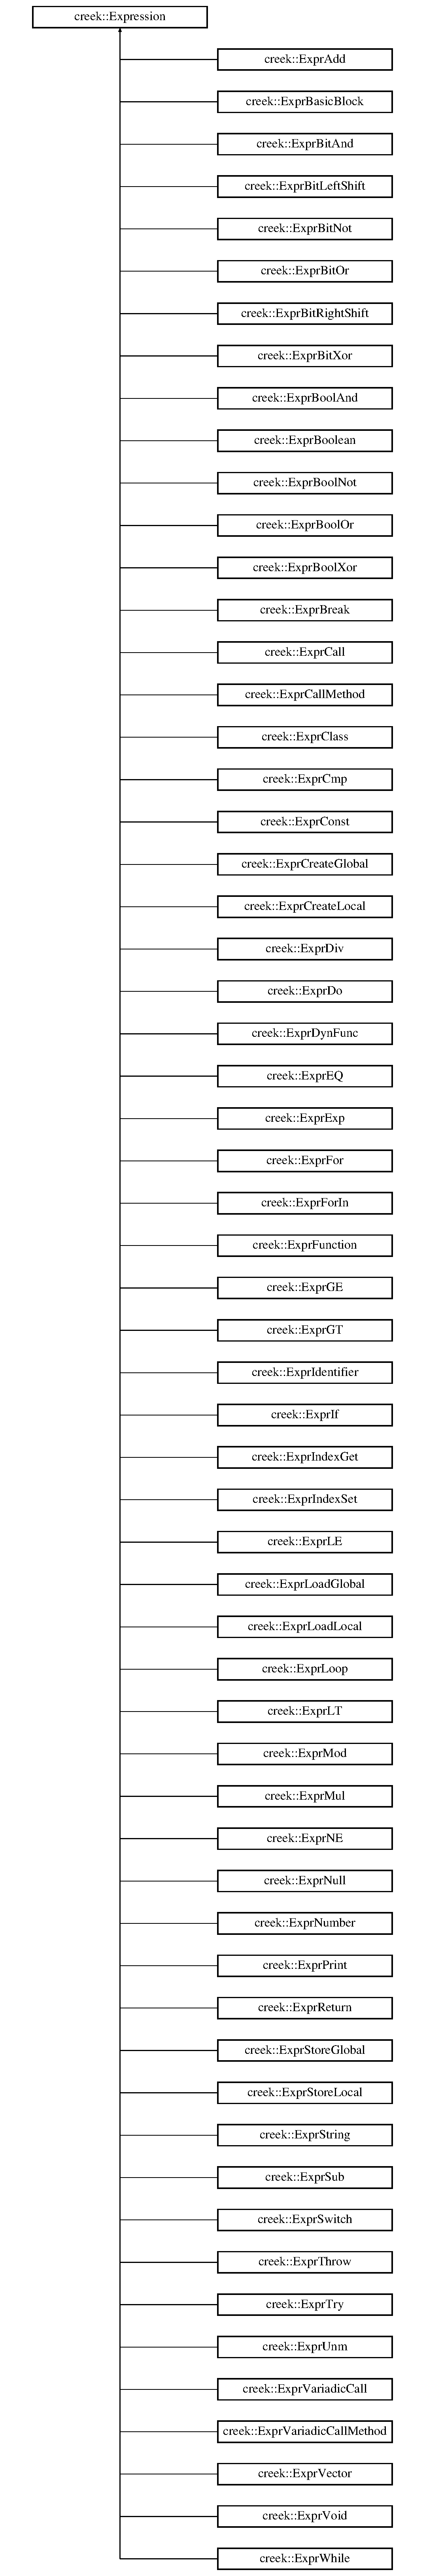
\includegraphics[height=12.000000cm]{classcreek_1_1_expression}
\end{center}
\end{figure}
\subsection*{Public Member Functions}
\begin{DoxyCompactItemize}
\item 
virtual \hyperlink{classcreek_1_1_variable}{Variable} \hyperlink{classcreek_1_1_expression_a3c7fe4a04e24c8d907f918240e2bf43d}{eval} (\hyperlink{classcreek_1_1_scope}{Scope} \&scope)=0
\begin{DoxyCompactList}\small\item\em Evaluate this expression. \end{DoxyCompactList}\item 
virtual bool \hyperlink{classcreek_1_1_expression_a657315f911348939ebedabfc258ff488}{is\+\_\+const} ()
\begin{DoxyCompactList}\small\item\em Check if this expression is constant. \end{DoxyCompactList}\item 
virtual \hyperlink{classcreek_1_1_bytecode}{Bytecode} \hyperlink{classcreek_1_1_expression_afd5d881693ecf750f264cde8cd49e446}{bytecode} (\hyperlink{classcreek_1_1_var_name_map}{Var\+Name\+Map} \&var\+\_\+name\+\_\+map) const  =0\hypertarget{classcreek_1_1_expression_afd5d881693ecf750f264cde8cd49e446}{}\label{classcreek_1_1_expression_afd5d881693ecf750f264cde8cd49e446}

\begin{DoxyCompactList}\small\item\em Get the bytecode of this expression. \end{DoxyCompactList}\end{DoxyCompactItemize}


\subsection{Detailed Description}
\hyperlink{classcreek_1_1_expression}{Expression} statement in a program. 

\subsection{Member Function Documentation}
\index{creek\+::\+Expression@{creek\+::\+Expression}!eval@{eval}}
\index{eval@{eval}!creek\+::\+Expression@{creek\+::\+Expression}}
\subsubsection[{\texorpdfstring{eval(\+Scope \&scope)=0}{eval(Scope &scope)=0}}]{\setlength{\rightskip}{0pt plus 5cm}virtual {\bf Variable} creek\+::\+Expression\+::eval (
\begin{DoxyParamCaption}
\item[{{\bf Scope} \&}]{scope}
\end{DoxyParamCaption}
)\hspace{0.3cm}{\ttfamily [pure virtual]}}\hypertarget{classcreek_1_1_expression_a3c7fe4a04e24c8d907f918240e2bf43d}{}\label{classcreek_1_1_expression_a3c7fe4a04e24c8d907f918240e2bf43d}


Evaluate this expression. 

\begin{DoxyReturn}{Returns}
Result of the expression; may be {\ttfamily nullptr}. 
\end{DoxyReturn}


Implemented in \hyperlink{classcreek_1_1_expr_break_a1111901c96f12e26e1ce3c483f2a7af5}{creek\+::\+Expr\+Break}, \hyperlink{classcreek_1_1_expr_return_a4f3c6f5a47a56cbb99599fadc3b63a4f}{creek\+::\+Expr\+Return}, \hyperlink{classcreek_1_1_expr_throw_a8402ea5b977841ae1733d0f76d7185bf}{creek\+::\+Expr\+Throw}, \hyperlink{classcreek_1_1_expr_class_abeac4981d65498ebfa385e1dae6b82da}{creek\+::\+Expr\+Class}, \hyperlink{classcreek_1_1_expr_try_a86c2677212b9cb689209cedf9196767c}{creek\+::\+Expr\+Try}, \hyperlink{classcreek_1_1_expr_for_in_a1ca1a4d1be979565174184945d7ed8ff}{creek\+::\+Expr\+For\+In}, \hyperlink{classcreek_1_1_expr_for_a98b3d4c28039a4b5f88917fd780727e2}{creek\+::\+Expr\+For}, \hyperlink{classcreek_1_1_expr_index_set_aafd64bba24bfe3b2a1cd6c4fa8dfaaee}{creek\+::\+Expr\+Index\+Set}, \hyperlink{classcreek_1_1_expr_function_a10f8cd65e471d823c68b81fc20435738}{creek\+::\+Expr\+Function}, \hyperlink{classcreek_1_1_expr_g_e_a3345b3022a238af6b09ae9fa1bd1584f}{creek\+::\+Expr\+GE}, \hyperlink{classcreek_1_1_expr_unm_a904e9e78ebed3f79b772f242fbca7fad}{creek\+::\+Expr\+Unm}, \hyperlink{classcreek_1_1_expr_while_a8a58de411d49efa90ccc6e1638964fbb}{creek\+::\+Expr\+While}, \hyperlink{classcreek_1_1_expr_vector_a10281fdb5c4f552c8f7d2abf85067315}{creek\+::\+Expr\+Vector}, \hyperlink{classcreek_1_1_expr_index_get_aa76e7e024f8c52560b222c0426c72e22}{creek\+::\+Expr\+Index\+Get}, \hyperlink{classcreek_1_1_expr_exp_a705ec2846acdc2923f6c75e13ef5dd3a}{creek\+::\+Expr\+Exp}, \hyperlink{classcreek_1_1_expr_g_t_a8207afd8212d5601ff92debfeee6330c}{creek\+::\+Expr\+GT}, \hyperlink{classcreek_1_1_expr_bit_right_shift_a3029e8ff6053b03a613bff438bceb1f1}{creek\+::\+Expr\+Bit\+Right\+Shift}, \hyperlink{classcreek_1_1_expr_loop_a150a70e174b15df925f3dbbbfb2aae2f}{creek\+::\+Expr\+Loop}, \hyperlink{classcreek_1_1_expr_store_global_a6d155c6e9892a9691963bc1008cf21e4}{creek\+::\+Expr\+Store\+Global}, \hyperlink{classcreek_1_1_expr_identifier_acb9cc26579b3dc0cd08f76685222df93}{creek\+::\+Expr\+Identifier}, \hyperlink{classcreek_1_1_expr_variadic_call_method_a19efdd6a56fd70f685b18ce4684c9113}{creek\+::\+Expr\+Variadic\+Call\+Method}, \hyperlink{classcreek_1_1_expr_mod_a974e82bd8d5475d0ccb581f8bcfa50f9}{creek\+::\+Expr\+Mod}, \hyperlink{classcreek_1_1_expr_l_e_a223206d456000e0587d69cca65816c8a}{creek\+::\+Expr\+LE}, \hyperlink{classcreek_1_1_expr_bit_left_shift_a77a8a9cb038e025d0627e94b8d8ec9f0}{creek\+::\+Expr\+Bit\+Left\+Shift}, \hyperlink{classcreek_1_1_expr_switch_a80d7830447263afc5a1acd27e770d47b}{creek\+::\+Expr\+Switch}, \hyperlink{classcreek_1_1_expr_load_global_a2ad646f205e977200f541208e33ebcae}{creek\+::\+Expr\+Load\+Global}, \hyperlink{classcreek_1_1_expr_string_a7db398cd35dcfc552a2c17e430cf1d1b}{creek\+::\+Expr\+String}, \hyperlink{classcreek_1_1_expr_l_t_a3a06f97fcdcc60b8e48c2649ac73b0ac}{creek\+::\+Expr\+LT}, \hyperlink{classcreek_1_1_expr_call_method_a8f3ba74247e00f1b531fd1f4415ec73f}{creek\+::\+Expr\+Call\+Method}, \hyperlink{classcreek_1_1_expr_div_a1fdc30ff0bca89f749073d3ebdd85040}{creek\+::\+Expr\+Div}, \hyperlink{classcreek_1_1_expr_bool_not_af7dedd20fe4da94bb9e1c246d45e90cb}{creek\+::\+Expr\+Bool\+Not}, \hyperlink{classcreek_1_1_expr_bit_not_aa8b898516fef2e8da32e660cc70f677e}{creek\+::\+Expr\+Bit\+Not}, \hyperlink{classcreek_1_1_expr_create_global_afb61097d41d367ea41be1cd66a3ef2bb}{creek\+::\+Expr\+Create\+Global}, \hyperlink{classcreek_1_1_expr_number_af9733eb2e8a6f30cdfe3fcf3029725e4}{creek\+::\+Expr\+Number}, \hyperlink{classcreek_1_1_expr_bool_xor_a16d8f13d6c8393ef58bf30b0bd9c53ae}{creek\+::\+Expr\+Bool\+Xor}, \hyperlink{classcreek_1_1_expr_n_e_ad0fc128b6060f2e9231fea49126f738f}{creek\+::\+Expr\+NE}, \hyperlink{classcreek_1_1_expr_mul_a285e95e75af0a5eea988b8b943057f82}{creek\+::\+Expr\+Mul}, \hyperlink{classcreek_1_1_expr_bit_xor_a291257ee80afb487e727858ae59fdee9}{creek\+::\+Expr\+Bit\+Xor}, \hyperlink{classcreek_1_1_expr_variadic_call_a5d797164553d7a1c631fa0a91a7656ad}{creek\+::\+Expr\+Variadic\+Call}, \hyperlink{classcreek_1_1_expr_if_a0aceaefe760432ec4404fd4bb2b95076}{creek\+::\+Expr\+If}, \hyperlink{classcreek_1_1_expr_store_local_ae61d30ec3ca4e9506d23a435875edb85}{creek\+::\+Expr\+Store\+Local}, \hyperlink{classcreek_1_1_expr_boolean_a23d54ae588f798e031539bb1e4ea7e47}{creek\+::\+Expr\+Boolean}, \hyperlink{classcreek_1_1_expr_e_q_a15063eb60b1cdd652f08ec7b6abf497d}{creek\+::\+Expr\+EQ}, \hyperlink{classcreek_1_1_expr_sub_a2b80d9d6dcfbab85df41674e73b02625}{creek\+::\+Expr\+Sub}, \hyperlink{classcreek_1_1_expr_bit_or_a9066c33c5d0f95d39d4bab927dfd9a93}{creek\+::\+Expr\+Bit\+Or}, \hyperlink{classcreek_1_1_expr_bool_or_a359cd14a552c56000e8b687c1e58df72}{creek\+::\+Expr\+Bool\+Or}, \hyperlink{classcreek_1_1_expr_null_a8f9e7c9e1e635b148936627bf33018a7}{creek\+::\+Expr\+Null}, \hyperlink{classcreek_1_1_expr_load_local_a0967bafe453441742d9469501388bb06}{creek\+::\+Expr\+Load\+Local}, \hyperlink{classcreek_1_1_expr_do_aebcd267e0a9ad22fcd9cef61901b12cb}{creek\+::\+Expr\+Do}, \hyperlink{classcreek_1_1_expr_call_a866b5e444449beae3332e224705b9c74}{creek\+::\+Expr\+Call}, \hyperlink{classcreek_1_1_expr_void_a298067bd586345ec4f7d716e9decaf5f}{creek\+::\+Expr\+Void}, \hyperlink{classcreek_1_1_expr_dyn_func_af04443b77329e7a075f02ff9efb08b56}{creek\+::\+Expr\+Dyn\+Func}, \hyperlink{classcreek_1_1_expr_basic_block_a95fe118d4b862d16640f002449cd4278}{creek\+::\+Expr\+Basic\+Block}, \hyperlink{classcreek_1_1_expr_cmp_a45d3b9bcf46c7ac302494cbda5caf49e}{creek\+::\+Expr\+Cmp}, \hyperlink{classcreek_1_1_expr_print_abcbd3bcb766342402937c5c5e38efcff}{creek\+::\+Expr\+Print}, \hyperlink{classcreek_1_1_expr_create_local_a1f3f2597f512437ec135c79d012e9ad8}{creek\+::\+Expr\+Create\+Local}, \hyperlink{classcreek_1_1_expr_add_a3d8ff369c865a75ff359adb85afc423f}{creek\+::\+Expr\+Add}, \hyperlink{classcreek_1_1_expr_bit_and_a59a8927267c2e7e2af9cc2b6ea757b93}{creek\+::\+Expr\+Bit\+And}, \hyperlink{classcreek_1_1_expr_bool_and_a10e710637b3ab561e83c420a858a6130}{creek\+::\+Expr\+Bool\+And}, and \hyperlink{classcreek_1_1_expr_const_ad5602ea2700ea4d6c1ce86457cb151a6}{creek\+::\+Expr\+Const}.

\index{creek\+::\+Expression@{creek\+::\+Expression}!is\+\_\+const@{is\+\_\+const}}
\index{is\+\_\+const@{is\+\_\+const}!creek\+::\+Expression@{creek\+::\+Expression}}
\subsubsection[{\texorpdfstring{is\+\_\+const()}{is_const()}}]{\setlength{\rightskip}{0pt plus 5cm}virtual bool creek\+::\+Expression\+::is\+\_\+const (
\begin{DoxyParamCaption}
{}
\end{DoxyParamCaption}
)\hspace{0.3cm}{\ttfamily [inline]}, {\ttfamily [virtual]}}\hypertarget{classcreek_1_1_expression_a657315f911348939ebedabfc258ff488}{}\label{classcreek_1_1_expression_a657315f911348939ebedabfc258ff488}


Check if this expression is constant. 

\begin{DoxyReturn}{Returns}
True if this expression can be evaluated at compile time. 
\end{DoxyReturn}


The documentation for this class was generated from the following file\+:\begin{DoxyCompactItemize}
\item 
C\+:/\+Users/\+Eric/\+Projects/\+Creek\+Script/bytecode/\+Creek\+Script/src/creek/Expression.\+hpp\end{DoxyCompactItemize}

\hypertarget{classcreek_1_1_expr_exp}{}\section{creek\+:\+:Expr\+Exp Class Reference}
\label{classcreek_1_1_expr_exp}\index{creek\+::\+Expr\+Exp@{creek\+::\+Expr\+Exp}}


{\ttfamily \#include $<$Expression\+\_\+\+Arithmetic.\+hpp$>$}

Inheritance diagram for creek\+:\+:Expr\+Exp\+:\begin{figure}[H]
\begin{center}
\leavevmode
\includegraphics[height=2.000000cm]{classcreek_1_1_expr_exp}
\end{center}
\end{figure}
\subsection*{Public Member Functions}
\begin{DoxyCompactItemize}
\item 
\hyperlink{classcreek_1_1_expr_exp_aa7c64f13997a13c1cdd2ddf7b1f6ed7c}{Expr\+Exp} (\hyperlink{classcreek_1_1_expression}{Expression} $\ast$lexpr, \hyperlink{classcreek_1_1_expression}{Expression} $\ast$rexpr)
\item 
\hyperlink{classcreek_1_1_variable}{Variable} \hyperlink{classcreek_1_1_expr_exp_a705ec2846acdc2923f6c75e13ef5dd3a}{eval} (\hyperlink{classcreek_1_1_scope}{Scope} \&scope) override
\begin{DoxyCompactList}\small\item\em Evaluate this expression. \end{DoxyCompactList}\item 
\hyperlink{classcreek_1_1_bytecode}{Bytecode} \hyperlink{classcreek_1_1_expr_exp_a07505cfa48dd3c10437562d561944b4a}{bytecode} (\hyperlink{classcreek_1_1_var_name_map}{Var\+Name\+Map} \&var\+\_\+name\+\_\+map) const  override\hypertarget{classcreek_1_1_expr_exp_a07505cfa48dd3c10437562d561944b4a}{}\label{classcreek_1_1_expr_exp_a07505cfa48dd3c10437562d561944b4a}

\begin{DoxyCompactList}\small\item\em Get the bytecode of this expression. \end{DoxyCompactList}\end{DoxyCompactItemize}


\subsection{Detailed Description}
\hyperlink{classcreek_1_1_expression}{Expression}\+: Exponentiate two values. Returns L $\ast$$\ast$ R. 

\subsection{Constructor \& Destructor Documentation}
\index{creek\+::\+Expr\+Exp@{creek\+::\+Expr\+Exp}!Expr\+Exp@{Expr\+Exp}}
\index{Expr\+Exp@{Expr\+Exp}!creek\+::\+Expr\+Exp@{creek\+::\+Expr\+Exp}}
\subsubsection[{\texorpdfstring{Expr\+Exp(\+Expression $\ast$lexpr, Expression $\ast$rexpr)}{ExprExp(Expression *lexpr, Expression *rexpr)}}]{\setlength{\rightskip}{0pt plus 5cm}creek\+::\+Expr\+Exp\+::\+Expr\+Exp (
\begin{DoxyParamCaption}
\item[{{\bf Expression} $\ast$}]{lexpr, }
\item[{{\bf Expression} $\ast$}]{rexpr}
\end{DoxyParamCaption}
)}\hypertarget{classcreek_1_1_expr_exp_aa7c64f13997a13c1cdd2ddf7b1f6ed7c}{}\label{classcreek_1_1_expr_exp_aa7c64f13997a13c1cdd2ddf7b1f6ed7c}
{\ttfamily \hyperlink{classcreek_1_1_expr_exp}{Expr\+Exp}} constructor. 
\begin{DoxyParams}{Parameters}
{\em lexpr} & \hyperlink{classcreek_1_1_expression}{Expression} for left parameter. \\
\hline
{\em rexpr} & \hyperlink{classcreek_1_1_expression}{Expression} for right parameter. \\
\hline
\end{DoxyParams}


\subsection{Member Function Documentation}
\index{creek\+::\+Expr\+Exp@{creek\+::\+Expr\+Exp}!eval@{eval}}
\index{eval@{eval}!creek\+::\+Expr\+Exp@{creek\+::\+Expr\+Exp}}
\subsubsection[{\texorpdfstring{eval(\+Scope \&scope) override}{eval(Scope &scope) override}}]{\setlength{\rightskip}{0pt plus 5cm}{\bf Variable} creek\+::\+Expr\+Exp\+::eval (
\begin{DoxyParamCaption}
\item[{{\bf Scope} \&}]{scope}
\end{DoxyParamCaption}
)\hspace{0.3cm}{\ttfamily [override]}, {\ttfamily [virtual]}}\hypertarget{classcreek_1_1_expr_exp_a705ec2846acdc2923f6c75e13ef5dd3a}{}\label{classcreek_1_1_expr_exp_a705ec2846acdc2923f6c75e13ef5dd3a}


Evaluate this expression. 

\begin{DoxyReturn}{Returns}
Result of the expression; may be {\ttfamily nullptr}. 
\end{DoxyReturn}


Implements \hyperlink{classcreek_1_1_expression_a3c7fe4a04e24c8d907f918240e2bf43d}{creek\+::\+Expression}.



The documentation for this class was generated from the following files\+:\begin{DoxyCompactItemize}
\item 
C\+:/\+Users/\+Eric/\+Projects/\+Creek\+Script/bytecode/\+Creek\+Script/src/creek/Expression\+\_\+\+Arithmetic.\+hpp\item 
C\+:/\+Users/\+Eric/\+Projects/\+Creek\+Script/bytecode/\+Creek\+Script/src/creek/Expression\+\_\+\+Arithmetic.\+cpp\end{DoxyCompactItemize}

\hypertarget{classcreek_1_1_expr_for}{}\section{creek\+:\+:Expr\+For Class Reference}
\label{classcreek_1_1_expr_for}\index{creek\+::\+Expr\+For@{creek\+::\+Expr\+For}}


{\ttfamily \#include $<$Expression\+\_\+\+Control\+Flow.\+hpp$>$}

Inheritance diagram for creek\+:\+:Expr\+For\+:\begin{figure}[H]
\begin{center}
\leavevmode
\includegraphics[height=2.000000cm]{classcreek_1_1_expr_for}
\end{center}
\end{figure}
\subsection*{Public Member Functions}
\begin{DoxyCompactItemize}
\item 
\hyperlink{classcreek_1_1_expr_for_aa3b329ab8038f74c5ad88273d7c006cc}{Expr\+For} (\hyperlink{classcreek_1_1_var_name}{Var\+Name} var\+\_\+name, \hyperlink{classcreek_1_1_expression}{Expression} $\ast$initial\+\_\+value, \hyperlink{classcreek_1_1_expression}{Expression} $\ast$max\+\_\+value, \hyperlink{classcreek_1_1_expression}{Expression} $\ast$step\+\_\+value, \hyperlink{classcreek_1_1_expression}{Expression} $\ast$body)
\item 
\hyperlink{classcreek_1_1_variable}{Variable} \hyperlink{classcreek_1_1_expr_for_a98b3d4c28039a4b5f88917fd780727e2}{eval} (\hyperlink{classcreek_1_1_scope}{Scope} \&scope) override
\begin{DoxyCompactList}\small\item\em Evaluate this expression. \end{DoxyCompactList}\item 
\hyperlink{classcreek_1_1_bytecode}{Bytecode} \hyperlink{classcreek_1_1_expr_for_a2f7159f87a5c432536b7c6018d3213e6}{bytecode} (\hyperlink{classcreek_1_1_var_name_map}{Var\+Name\+Map} \&var\+\_\+name\+\_\+map) const  override\hypertarget{classcreek_1_1_expr_for_a2f7159f87a5c432536b7c6018d3213e6}{}\label{classcreek_1_1_expr_for_a2f7159f87a5c432536b7c6018d3213e6}

\begin{DoxyCompactList}\small\item\em Get the bytecode of this expression. \end{DoxyCompactList}\end{DoxyCompactItemize}


\subsection{Detailed Description}
\hyperlink{classcreek_1_1_expression}{Expression}\+: Value based for loop. Returns result of last evaluated expression in the body, or void. 

\subsection{Constructor \& Destructor Documentation}
\index{creek\+::\+Expr\+For@{creek\+::\+Expr\+For}!Expr\+For@{Expr\+For}}
\index{Expr\+For@{Expr\+For}!creek\+::\+Expr\+For@{creek\+::\+Expr\+For}}
\subsubsection[{\texorpdfstring{Expr\+For(\+Var\+Name var\+\_\+name, Expression $\ast$initial\+\_\+value, Expression $\ast$max\+\_\+value, Expression $\ast$step\+\_\+value, Expression $\ast$body)}{ExprFor(VarName var_name, Expression *initial_value, Expression *max_value, Expression *step_value, Expression *body)}}]{\setlength{\rightskip}{0pt plus 5cm}creek\+::\+Expr\+For\+::\+Expr\+For (
\begin{DoxyParamCaption}
\item[{{\bf Var\+Name}}]{var\+\_\+name, }
\item[{{\bf Expression} $\ast$}]{initial\+\_\+value, }
\item[{{\bf Expression} $\ast$}]{max\+\_\+value, }
\item[{{\bf Expression} $\ast$}]{step\+\_\+value, }
\item[{{\bf Expression} $\ast$}]{body}
\end{DoxyParamCaption}
)}\hypertarget{classcreek_1_1_expr_for_aa3b329ab8038f74c5ad88273d7c006cc}{}\label{classcreek_1_1_expr_for_aa3b329ab8038f74c5ad88273d7c006cc}
{\ttfamily \hyperlink{classcreek_1_1_expr_for}{Expr\+For}} constructor. 
\begin{DoxyParams}{Parameters}
{\em var\+\_\+name} & \hyperlink{classcreek_1_1_variable}{Variable} name for the iterator. \\
\hline
{\em initial\+\_\+value} & Initial value of the iterator. \\
\hline
{\em max\+\_\+value} & Iterator must be less-\/than this. \\
\hline
{\em step\+\_\+value} & Iterator increment. \\
\hline
{\em body} & \hyperlink{classcreek_1_1_expression}{Expression} to execute in each loop. \\
\hline
\end{DoxyParams}


\subsection{Member Function Documentation}
\index{creek\+::\+Expr\+For@{creek\+::\+Expr\+For}!eval@{eval}}
\index{eval@{eval}!creek\+::\+Expr\+For@{creek\+::\+Expr\+For}}
\subsubsection[{\texorpdfstring{eval(\+Scope \&scope) override}{eval(Scope &scope) override}}]{\setlength{\rightskip}{0pt plus 5cm}{\bf Variable} creek\+::\+Expr\+For\+::eval (
\begin{DoxyParamCaption}
\item[{{\bf Scope} \&}]{scope}
\end{DoxyParamCaption}
)\hspace{0.3cm}{\ttfamily [override]}, {\ttfamily [virtual]}}\hypertarget{classcreek_1_1_expr_for_a98b3d4c28039a4b5f88917fd780727e2}{}\label{classcreek_1_1_expr_for_a98b3d4c28039a4b5f88917fd780727e2}


Evaluate this expression. 

\begin{DoxyReturn}{Returns}
Result of the expression; may be {\ttfamily nullptr}. 
\end{DoxyReturn}


Implements \hyperlink{classcreek_1_1_expression_a3c7fe4a04e24c8d907f918240e2bf43d}{creek\+::\+Expression}.



The documentation for this class was generated from the following files\+:\begin{DoxyCompactItemize}
\item 
C\+:/\+Users/\+Eric/\+Projects/\+Creek\+Script/bytecode/\+Creek\+Script/src/creek/Expression\+\_\+\+Control\+Flow.\+hpp\item 
C\+:/\+Users/\+Eric/\+Projects/\+Creek\+Script/bytecode/\+Creek\+Script/src/creek/Expression\+\_\+\+Control\+Flow.\+cpp\end{DoxyCompactItemize}

\hypertarget{classcreek_1_1_expr_for_in}{}\section{creek\+:\+:Expr\+For\+In Class Reference}
\label{classcreek_1_1_expr_for_in}\index{creek\+::\+Expr\+For\+In@{creek\+::\+Expr\+For\+In}}


{\ttfamily \#include $<$Expression\+\_\+\+Control\+Flow.\+hpp$>$}

Inheritance diagram for creek\+:\+:Expr\+For\+In\+:\begin{figure}[H]
\begin{center}
\leavevmode
\includegraphics[height=2.000000cm]{classcreek_1_1_expr_for_in}
\end{center}
\end{figure}
\subsection*{Public Member Functions}
\begin{DoxyCompactItemize}
\item 
\hyperlink{classcreek_1_1_expr_for_in_aa1878abf03240778957f7b3ebcff68f5}{Expr\+For\+In} (\hyperlink{classcreek_1_1_var_name}{Var\+Name} var\+\_\+name, \hyperlink{classcreek_1_1_expression}{Expression} $\ast$range, \hyperlink{classcreek_1_1_expression}{Expression} $\ast$body)
\item 
\hyperlink{classcreek_1_1_variable}{Variable} \hyperlink{classcreek_1_1_expr_for_in_a1ca1a4d1be979565174184945d7ed8ff}{eval} (\hyperlink{classcreek_1_1_scope}{Scope} \&scope) override
\begin{DoxyCompactList}\small\item\em Evaluate this expression. \end{DoxyCompactList}\item 
\hyperlink{classcreek_1_1_bytecode}{Bytecode} \hyperlink{classcreek_1_1_expr_for_in_a67aab389d085f616822e45f2a4b14ac3}{bytecode} (\hyperlink{classcreek_1_1_var_name_map}{Var\+Name\+Map} \&var\+\_\+name\+\_\+map) const  override\hypertarget{classcreek_1_1_expr_for_in_a67aab389d085f616822e45f2a4b14ac3}{}\label{classcreek_1_1_expr_for_in_a67aab389d085f616822e45f2a4b14ac3}

\begin{DoxyCompactList}\small\item\em Get the bytecode of this expression. \end{DoxyCompactList}\end{DoxyCompactItemize}


\subsection{Detailed Description}
\hyperlink{classcreek_1_1_expression}{Expression}\+: Range based for loop. Returns result of last evaluated expression in the body, or void. 

\subsection{Constructor \& Destructor Documentation}
\index{creek\+::\+Expr\+For\+In@{creek\+::\+Expr\+For\+In}!Expr\+For\+In@{Expr\+For\+In}}
\index{Expr\+For\+In@{Expr\+For\+In}!creek\+::\+Expr\+For\+In@{creek\+::\+Expr\+For\+In}}
\subsubsection[{\texorpdfstring{Expr\+For\+In(\+Var\+Name var\+\_\+name, Expression $\ast$range, Expression $\ast$body)}{ExprForIn(VarName var_name, Expression *range, Expression *body)}}]{\setlength{\rightskip}{0pt plus 5cm}creek\+::\+Expr\+For\+In\+::\+Expr\+For\+In (
\begin{DoxyParamCaption}
\item[{{\bf Var\+Name}}]{var\+\_\+name, }
\item[{{\bf Expression} $\ast$}]{range, }
\item[{{\bf Expression} $\ast$}]{body}
\end{DoxyParamCaption}
)}\hypertarget{classcreek_1_1_expr_for_in_aa1878abf03240778957f7b3ebcff68f5}{}\label{classcreek_1_1_expr_for_in_aa1878abf03240778957f7b3ebcff68f5}
{\ttfamily \hyperlink{classcreek_1_1_expr_for_in}{Expr\+For\+In}} constructor. 
\begin{DoxyParams}{Parameters}
{\em var\+\_\+name} & \hyperlink{classcreek_1_1_variable}{Variable} name for the iterator. \\
\hline
{\em range} & Range expression. \\
\hline
{\em body} & \hyperlink{classcreek_1_1_expression}{Expression} to execute in each loop. \\
\hline
\end{DoxyParams}


\subsection{Member Function Documentation}
\index{creek\+::\+Expr\+For\+In@{creek\+::\+Expr\+For\+In}!eval@{eval}}
\index{eval@{eval}!creek\+::\+Expr\+For\+In@{creek\+::\+Expr\+For\+In}}
\subsubsection[{\texorpdfstring{eval(\+Scope \&scope) override}{eval(Scope &scope) override}}]{\setlength{\rightskip}{0pt plus 5cm}{\bf Variable} creek\+::\+Expr\+For\+In\+::eval (
\begin{DoxyParamCaption}
\item[{{\bf Scope} \&}]{scope}
\end{DoxyParamCaption}
)\hspace{0.3cm}{\ttfamily [override]}, {\ttfamily [virtual]}}\hypertarget{classcreek_1_1_expr_for_in_a1ca1a4d1be979565174184945d7ed8ff}{}\label{classcreek_1_1_expr_for_in_a1ca1a4d1be979565174184945d7ed8ff}


Evaluate this expression. 

\begin{DoxyReturn}{Returns}
Result of the expression; may be {\ttfamily nullptr}. 
\end{DoxyReturn}


Implements \hyperlink{classcreek_1_1_expression_a3c7fe4a04e24c8d907f918240e2bf43d}{creek\+::\+Expression}.



The documentation for this class was generated from the following files\+:\begin{DoxyCompactItemize}
\item 
C\+:/\+Users/\+Eric/\+Projects/\+Creek\+Script/bytecode/\+Creek\+Script/src/creek/Expression\+\_\+\+Control\+Flow.\+hpp\item 
C\+:/\+Users/\+Eric/\+Projects/\+Creek\+Script/bytecode/\+Creek\+Script/src/creek/Expression\+\_\+\+Control\+Flow.\+cpp\end{DoxyCompactItemize}

\hypertarget{classcreek_1_1_expr_function}{}\section{creek\+:\+:Expr\+Function Class Reference}
\label{classcreek_1_1_expr_function}\index{creek\+::\+Expr\+Function@{creek\+::\+Expr\+Function}}


\hyperlink{classcreek_1_1_expression}{Expression}\+: Create a function data. Returns a new {\ttfamily \hyperlink{classcreek_1_1_function}{Function}}.  




{\ttfamily \#include $<$Expression\+\_\+\+Data\+Types.\+hpp$>$}

Inheritance diagram for creek\+:\+:Expr\+Function\+:\begin{figure}[H]
\begin{center}
\leavevmode
\includegraphics[height=2.000000cm]{classcreek_1_1_expr_function}
\end{center}
\end{figure}
\subsection*{Public Member Functions}
\begin{DoxyCompactItemize}
\item 
\hyperlink{classcreek_1_1_expr_function_a876b7e64e0864d3e34c349960dbf9450}{Expr\+Function} (const std\+::vector$<$ \hyperlink{classcreek_1_1_var_name}{Var\+Name} $>$ \&arg\+\_\+names, bool variadic, \hyperlink{classcreek_1_1_expression}{Expression} $\ast$body)
\item 
\hyperlink{classcreek_1_1_variable}{Variable} \hyperlink{classcreek_1_1_expr_function_a10f8cd65e471d823c68b81fc20435738}{eval} (\hyperlink{classcreek_1_1_scope}{Scope} \&scope) override
\begin{DoxyCompactList}\small\item\em Evaluate this expression. \end{DoxyCompactList}\item 
\hyperlink{classcreek_1_1_bytecode}{Bytecode} \hyperlink{classcreek_1_1_expr_function_abfed3d24bd0649351fa30bd608b87f1b}{bytecode} (\hyperlink{classcreek_1_1_var_name_map}{Var\+Name\+Map} \&var\+\_\+name\+\_\+map) const  override\hypertarget{classcreek_1_1_expr_function_abfed3d24bd0649351fa30bd608b87f1b}{}\label{classcreek_1_1_expr_function_abfed3d24bd0649351fa30bd608b87f1b}

\begin{DoxyCompactList}\small\item\em Get the bytecode of this expression. \end{DoxyCompactList}\end{DoxyCompactItemize}


\subsection{Detailed Description}
\hyperlink{classcreek_1_1_expression}{Expression}\+: Create a function data. Returns a new {\ttfamily \hyperlink{classcreek_1_1_function}{Function}}. 

\subsection{Constructor \& Destructor Documentation}
\index{creek\+::\+Expr\+Function@{creek\+::\+Expr\+Function}!Expr\+Function@{Expr\+Function}}
\index{Expr\+Function@{Expr\+Function}!creek\+::\+Expr\+Function@{creek\+::\+Expr\+Function}}
\subsubsection[{\texorpdfstring{Expr\+Function(const std\+::vector$<$ Var\+Name $>$ \&arg\+\_\+names, bool variadic, Expression $\ast$body)}{ExprFunction(const std::vector< VarName > &arg_names, bool variadic, Expression *body)}}]{\setlength{\rightskip}{0pt plus 5cm}creek\+::\+Expr\+Function\+::\+Expr\+Function (
\begin{DoxyParamCaption}
\item[{const std\+::vector$<$ {\bf Var\+Name} $>$ \&}]{arg\+\_\+names, }
\item[{bool}]{variadic, }
\item[{{\bf Expression} $\ast$}]{body}
\end{DoxyParamCaption}
)}\hypertarget{classcreek_1_1_expr_function_a876b7e64e0864d3e34c349960dbf9450}{}\label{classcreek_1_1_expr_function_a876b7e64e0864d3e34c349960dbf9450}
{\ttfamily \hyperlink{classcreek_1_1_expr_function}{Expr\+Function}} constructor. 
\begin{DoxyParams}{Parameters}
{\em arg\+\_\+names} & Names of arguments. \\
\hline
{\em variadic} & Create a variadic function. \\
\hline
{\em body} & \hyperlink{classcreek_1_1_function}{Function} body block. \\
\hline
\end{DoxyParams}


\subsection{Member Function Documentation}
\index{creek\+::\+Expr\+Function@{creek\+::\+Expr\+Function}!eval@{eval}}
\index{eval@{eval}!creek\+::\+Expr\+Function@{creek\+::\+Expr\+Function}}
\subsubsection[{\texorpdfstring{eval(\+Scope \&scope) override}{eval(Scope &scope) override}}]{\setlength{\rightskip}{0pt plus 5cm}{\bf Variable} creek\+::\+Expr\+Function\+::eval (
\begin{DoxyParamCaption}
\item[{{\bf Scope} \&}]{scope}
\end{DoxyParamCaption}
)\hspace{0.3cm}{\ttfamily [override]}, {\ttfamily [virtual]}}\hypertarget{classcreek_1_1_expr_function_a10f8cd65e471d823c68b81fc20435738}{}\label{classcreek_1_1_expr_function_a10f8cd65e471d823c68b81fc20435738}


Evaluate this expression. 

\begin{DoxyReturn}{Returns}
Result of the expression; may be {\ttfamily nullptr}. 
\end{DoxyReturn}


Implements \hyperlink{classcreek_1_1_expression_a3c7fe4a04e24c8d907f918240e2bf43d}{creek\+::\+Expression}.



The documentation for this class was generated from the following files\+:\begin{DoxyCompactItemize}
\item 
C\+:/\+Users/\+Eric/\+Projects/\+Creek\+Script/bytecode/\+Creek\+Script/src/creek/Expression\+\_\+\+Data\+Types.\+hpp\item 
C\+:/\+Users/\+Eric/\+Projects/\+Creek\+Script/bytecode/\+Creek\+Script/src/creek/Expression\+\_\+\+Data\+Types.\+cpp\end{DoxyCompactItemize}

\hypertarget{classcreek_1_1_expr_g_e}{}\section{creek\+:\+:Expr\+GE Class Reference}
\label{classcreek_1_1_expr_g_e}\index{creek\+::\+Expr\+GE@{creek\+::\+Expr\+GE}}


{\ttfamily \#include $<$Expression\+\_\+\+Comparison.\+hpp$>$}

Inheritance diagram for creek\+:\+:Expr\+GE\+:\begin{figure}[H]
\begin{center}
\leavevmode
\includegraphics[height=2.000000cm]{classcreek_1_1_expr_g_e}
\end{center}
\end{figure}
\subsection*{Public Member Functions}
\begin{DoxyCompactItemize}
\item 
\hyperlink{classcreek_1_1_expr_g_e_afead8cd6f0aac0d01e0a45a1762eb7c0}{Expr\+GE} (\hyperlink{classcreek_1_1_expression}{Expression} $\ast$lexpr, \hyperlink{classcreek_1_1_expression}{Expression} $\ast$rexpr)
\item 
\hyperlink{classcreek_1_1_variable}{Variable} \hyperlink{classcreek_1_1_expr_g_e_a3345b3022a238af6b09ae9fa1bd1584f}{eval} (\hyperlink{classcreek_1_1_scope}{Scope} \&scope) override
\begin{DoxyCompactList}\small\item\em Evaluate this expression. \end{DoxyCompactList}\item 
\hyperlink{classcreek_1_1_bytecode}{Bytecode} \hyperlink{classcreek_1_1_expr_g_e_a9b87dca5b84909cf71cfc8befe623f2d}{bytecode} (\hyperlink{classcreek_1_1_var_name_map}{Var\+Name\+Map} \&var\+\_\+name\+\_\+map) const  override\hypertarget{classcreek_1_1_expr_g_e_a9b87dca5b84909cf71cfc8befe623f2d}{}\label{classcreek_1_1_expr_g_e_a9b87dca5b84909cf71cfc8befe623f2d}

\begin{DoxyCompactList}\small\item\em Get the bytecode of this expression. \end{DoxyCompactList}\end{DoxyCompactItemize}


\subsection{Detailed Description}
\hyperlink{classcreek_1_1_expression}{Expression}\+: Greater than or equal to. Returns L $>$= R. 

\subsection{Constructor \& Destructor Documentation}
\index{creek\+::\+Expr\+GE@{creek\+::\+Expr\+GE}!Expr\+GE@{Expr\+GE}}
\index{Expr\+GE@{Expr\+GE}!creek\+::\+Expr\+GE@{creek\+::\+Expr\+GE}}
\subsubsection[{\texorpdfstring{Expr\+G\+E(\+Expression $\ast$lexpr, Expression $\ast$rexpr)}{ExprGE(Expression *lexpr, Expression *rexpr)}}]{\setlength{\rightskip}{0pt plus 5cm}creek\+::\+Expr\+G\+E\+::\+Expr\+GE (
\begin{DoxyParamCaption}
\item[{{\bf Expression} $\ast$}]{lexpr, }
\item[{{\bf Expression} $\ast$}]{rexpr}
\end{DoxyParamCaption}
)}\hypertarget{classcreek_1_1_expr_g_e_afead8cd6f0aac0d01e0a45a1762eb7c0}{}\label{classcreek_1_1_expr_g_e_afead8cd6f0aac0d01e0a45a1762eb7c0}
{\ttfamily \hyperlink{classcreek_1_1_expr_g_e}{Expr\+GE}} constructor. 
\begin{DoxyParams}{Parameters}
{\em lexpr} & \hyperlink{classcreek_1_1_expression}{Expression} for left parameter. \\
\hline
{\em rexpr} & \hyperlink{classcreek_1_1_expression}{Expression} for right parameter. \\
\hline
\end{DoxyParams}


\subsection{Member Function Documentation}
\index{creek\+::\+Expr\+GE@{creek\+::\+Expr\+GE}!eval@{eval}}
\index{eval@{eval}!creek\+::\+Expr\+GE@{creek\+::\+Expr\+GE}}
\subsubsection[{\texorpdfstring{eval(\+Scope \&scope) override}{eval(Scope &scope) override}}]{\setlength{\rightskip}{0pt plus 5cm}{\bf Variable} creek\+::\+Expr\+G\+E\+::eval (
\begin{DoxyParamCaption}
\item[{{\bf Scope} \&}]{scope}
\end{DoxyParamCaption}
)\hspace{0.3cm}{\ttfamily [override]}, {\ttfamily [virtual]}}\hypertarget{classcreek_1_1_expr_g_e_a3345b3022a238af6b09ae9fa1bd1584f}{}\label{classcreek_1_1_expr_g_e_a3345b3022a238af6b09ae9fa1bd1584f}


Evaluate this expression. 

\begin{DoxyReturn}{Returns}
Result of the expression; may be {\ttfamily nullptr}. 
\end{DoxyReturn}


Implements \hyperlink{classcreek_1_1_expression_a3c7fe4a04e24c8d907f918240e2bf43d}{creek\+::\+Expression}.



The documentation for this class was generated from the following files\+:\begin{DoxyCompactItemize}
\item 
C\+:/\+Users/\+Eric/\+Projects/\+Creek\+Script/bytecode/\+Creek\+Script/src/creek/Expression\+\_\+\+Comparison.\+hpp\item 
C\+:/\+Users/\+Eric/\+Projects/\+Creek\+Script/bytecode/\+Creek\+Script/src/creek/Expression\+\_\+\+Comparison.\+cpp\end{DoxyCompactItemize}

\hypertarget{classcreek_1_1_expr_g_t}{}\section{creek\+:\+:Expr\+GT Class Reference}
\label{classcreek_1_1_expr_g_t}\index{creek\+::\+Expr\+GT@{creek\+::\+Expr\+GT}}


{\ttfamily \#include $<$Expression\+\_\+\+Comparison.\+hpp$>$}

Inheritance diagram for creek\+:\+:Expr\+GT\+:\begin{figure}[H]
\begin{center}
\leavevmode
\includegraphics[height=2.000000cm]{classcreek_1_1_expr_g_t}
\end{center}
\end{figure}
\subsection*{Public Member Functions}
\begin{DoxyCompactItemize}
\item 
\hyperlink{classcreek_1_1_expr_g_t_a213248f67e90f13a1859b21f21de70b9}{Expr\+GT} (\hyperlink{classcreek_1_1_expression}{Expression} $\ast$lexpr, \hyperlink{classcreek_1_1_expression}{Expression} $\ast$rexpr)
\item 
\hyperlink{classcreek_1_1_variable}{Variable} \hyperlink{classcreek_1_1_expr_g_t_a8207afd8212d5601ff92debfeee6330c}{eval} (\hyperlink{classcreek_1_1_scope}{Scope} \&scope) override
\begin{DoxyCompactList}\small\item\em Evaluate this expression. \end{DoxyCompactList}\item 
\hyperlink{classcreek_1_1_bytecode}{Bytecode} \hyperlink{classcreek_1_1_expr_g_t_a0eda241e2dd10848b1a3a2097ff56cb3}{bytecode} (\hyperlink{classcreek_1_1_var_name_map}{Var\+Name\+Map} \&var\+\_\+name\+\_\+map) const  override\hypertarget{classcreek_1_1_expr_g_t_a0eda241e2dd10848b1a3a2097ff56cb3}{}\label{classcreek_1_1_expr_g_t_a0eda241e2dd10848b1a3a2097ff56cb3}

\begin{DoxyCompactList}\small\item\em Get the bytecode of this expression. \end{DoxyCompactList}\end{DoxyCompactItemize}


\subsection{Detailed Description}
\hyperlink{classcreek_1_1_expression}{Expression}\+: Greater than. Returns L $>$ R. 

\subsection{Constructor \& Destructor Documentation}
\index{creek\+::\+Expr\+GT@{creek\+::\+Expr\+GT}!Expr\+GT@{Expr\+GT}}
\index{Expr\+GT@{Expr\+GT}!creek\+::\+Expr\+GT@{creek\+::\+Expr\+GT}}
\subsubsection[{\texorpdfstring{Expr\+G\+T(\+Expression $\ast$lexpr, Expression $\ast$rexpr)}{ExprGT(Expression *lexpr, Expression *rexpr)}}]{\setlength{\rightskip}{0pt plus 5cm}creek\+::\+Expr\+G\+T\+::\+Expr\+GT (
\begin{DoxyParamCaption}
\item[{{\bf Expression} $\ast$}]{lexpr, }
\item[{{\bf Expression} $\ast$}]{rexpr}
\end{DoxyParamCaption}
)}\hypertarget{classcreek_1_1_expr_g_t_a213248f67e90f13a1859b21f21de70b9}{}\label{classcreek_1_1_expr_g_t_a213248f67e90f13a1859b21f21de70b9}
{\ttfamily \hyperlink{classcreek_1_1_expr_g_t}{Expr\+GT}} constructor. 
\begin{DoxyParams}{Parameters}
{\em lexpr} & \hyperlink{classcreek_1_1_expression}{Expression} for left parameter. \\
\hline
{\em rexpr} & \hyperlink{classcreek_1_1_expression}{Expression} for right parameter. \\
\hline
\end{DoxyParams}


\subsection{Member Function Documentation}
\index{creek\+::\+Expr\+GT@{creek\+::\+Expr\+GT}!eval@{eval}}
\index{eval@{eval}!creek\+::\+Expr\+GT@{creek\+::\+Expr\+GT}}
\subsubsection[{\texorpdfstring{eval(\+Scope \&scope) override}{eval(Scope &scope) override}}]{\setlength{\rightskip}{0pt plus 5cm}{\bf Variable} creek\+::\+Expr\+G\+T\+::eval (
\begin{DoxyParamCaption}
\item[{{\bf Scope} \&}]{scope}
\end{DoxyParamCaption}
)\hspace{0.3cm}{\ttfamily [override]}, {\ttfamily [virtual]}}\hypertarget{classcreek_1_1_expr_g_t_a8207afd8212d5601ff92debfeee6330c}{}\label{classcreek_1_1_expr_g_t_a8207afd8212d5601ff92debfeee6330c}


Evaluate this expression. 

\begin{DoxyReturn}{Returns}
Result of the expression; may be {\ttfamily nullptr}. 
\end{DoxyReturn}


Implements \hyperlink{classcreek_1_1_expression_a3c7fe4a04e24c8d907f918240e2bf43d}{creek\+::\+Expression}.



The documentation for this class was generated from the following files\+:\begin{DoxyCompactItemize}
\item 
C\+:/\+Users/\+Eric/\+Projects/\+Creek\+Script/bytecode/\+Creek\+Script/src/creek/Expression\+\_\+\+Comparison.\+hpp\item 
C\+:/\+Users/\+Eric/\+Projects/\+Creek\+Script/bytecode/\+Creek\+Script/src/creek/Expression\+\_\+\+Comparison.\+cpp\end{DoxyCompactItemize}

\hypertarget{classcreek_1_1_expr_identifier}{}\section{creek\+:\+:Expr\+Identifier Class Reference}
\label{classcreek_1_1_expr_identifier}\index{creek\+::\+Expr\+Identifier@{creek\+::\+Expr\+Identifier}}


\hyperlink{classcreek_1_1_expression}{Expression}\+: Create a identifier data. Returns a new {\ttfamily \hyperlink{classcreek_1_1_identifier}{Identifier}}.  




{\ttfamily \#include $<$Expression\+\_\+\+Data\+Types.\+hpp$>$}

Inheritance diagram for creek\+:\+:Expr\+Identifier\+:\begin{figure}[H]
\begin{center}
\leavevmode
\includegraphics[height=2.000000cm]{classcreek_1_1_expr_identifier}
\end{center}
\end{figure}
\subsection*{Public Member Functions}
\begin{DoxyCompactItemize}
\item 
\hyperlink{classcreek_1_1_expr_identifier_abcd8ce58f7ea6b03c20fbc0337556a8e}{Expr\+Identifier} (\hyperlink{classcreek_1_1_identifier_afb560a4cce99e96c30092edbd22a5ef4}{Identifier\+::\+Value} value)
\item 
\hyperlink{classcreek_1_1_variable}{Variable} \hyperlink{classcreek_1_1_expr_identifier_acb9cc26579b3dc0cd08f76685222df93}{eval} (\hyperlink{classcreek_1_1_scope}{Scope} \&scope) override
\begin{DoxyCompactList}\small\item\em Evaluate this expression. \end{DoxyCompactList}\item 
\hyperlink{classcreek_1_1_bytecode}{Bytecode} \hyperlink{classcreek_1_1_expr_identifier_a749f8b0d36a805c7a28d0c1acd737315}{bytecode} (\hyperlink{classcreek_1_1_var_name_map}{Var\+Name\+Map} \&var\+\_\+name\+\_\+map) const  override\hypertarget{classcreek_1_1_expr_identifier_a749f8b0d36a805c7a28d0c1acd737315}{}\label{classcreek_1_1_expr_identifier_a749f8b0d36a805c7a28d0c1acd737315}

\begin{DoxyCompactList}\small\item\em Get the bytecode of this expression. \end{DoxyCompactList}\end{DoxyCompactItemize}


\subsection{Detailed Description}
\hyperlink{classcreek_1_1_expression}{Expression}\+: Create a identifier data. Returns a new {\ttfamily \hyperlink{classcreek_1_1_identifier}{Identifier}}. 

\subsection{Constructor \& Destructor Documentation}
\index{creek\+::\+Expr\+Identifier@{creek\+::\+Expr\+Identifier}!Expr\+Identifier@{Expr\+Identifier}}
\index{Expr\+Identifier@{Expr\+Identifier}!creek\+::\+Expr\+Identifier@{creek\+::\+Expr\+Identifier}}
\subsubsection[{\texorpdfstring{Expr\+Identifier(\+Identifier\+::\+Value value)}{ExprIdentifier(Identifier::Value value)}}]{\setlength{\rightskip}{0pt plus 5cm}creek\+::\+Expr\+Identifier\+::\+Expr\+Identifier (
\begin{DoxyParamCaption}
\item[{{\bf Identifier\+::\+Value}}]{value}
\end{DoxyParamCaption}
)}\hypertarget{classcreek_1_1_expr_identifier_abcd8ce58f7ea6b03c20fbc0337556a8e}{}\label{classcreek_1_1_expr_identifier_abcd8ce58f7ea6b03c20fbc0337556a8e}
{\ttfamily \hyperlink{classcreek_1_1_expr_identifier}{Expr\+Identifier}} constructor. 
\begin{DoxyParams}{Parameters}
{\em value} & \hyperlink{classcreek_1_1_identifier}{Identifier} value. \\
\hline
\end{DoxyParams}


\subsection{Member Function Documentation}
\index{creek\+::\+Expr\+Identifier@{creek\+::\+Expr\+Identifier}!eval@{eval}}
\index{eval@{eval}!creek\+::\+Expr\+Identifier@{creek\+::\+Expr\+Identifier}}
\subsubsection[{\texorpdfstring{eval(\+Scope \&scope) override}{eval(Scope &scope) override}}]{\setlength{\rightskip}{0pt plus 5cm}{\bf Variable} creek\+::\+Expr\+Identifier\+::eval (
\begin{DoxyParamCaption}
\item[{{\bf Scope} \&}]{scope}
\end{DoxyParamCaption}
)\hspace{0.3cm}{\ttfamily [override]}, {\ttfamily [virtual]}}\hypertarget{classcreek_1_1_expr_identifier_acb9cc26579b3dc0cd08f76685222df93}{}\label{classcreek_1_1_expr_identifier_acb9cc26579b3dc0cd08f76685222df93}


Evaluate this expression. 

\begin{DoxyReturn}{Returns}
Result of the expression; may be {\ttfamily nullptr}. 
\end{DoxyReturn}


Implements \hyperlink{classcreek_1_1_expression_a3c7fe4a04e24c8d907f918240e2bf43d}{creek\+::\+Expression}.



The documentation for this class was generated from the following files\+:\begin{DoxyCompactItemize}
\item 
C\+:/\+Users/\+Eric/\+Projects/\+Creek\+Script/bytecode/\+Creek\+Script/src/creek/Expression\+\_\+\+Data\+Types.\+hpp\item 
C\+:/\+Users/\+Eric/\+Projects/\+Creek\+Script/bytecode/\+Creek\+Script/src/creek/Expression\+\_\+\+Data\+Types.\+cpp\end{DoxyCompactItemize}

\hypertarget{classcreek_1_1_expr_if}{}\section{creek\+:\+:Expr\+If Class Reference}
\label{classcreek_1_1_expr_if}\index{creek\+::\+Expr\+If@{creek\+::\+Expr\+If}}


{\ttfamily \#include $<$Expression\+\_\+\+Control\+Flow.\+hpp$>$}

Inheritance diagram for creek\+:\+:Expr\+If\+:\begin{figure}[H]
\begin{center}
\leavevmode
\includegraphics[height=2.000000cm]{classcreek_1_1_expr_if}
\end{center}
\end{figure}
\subsection*{Public Member Functions}
\begin{DoxyCompactItemize}
\item 
\hyperlink{classcreek_1_1_expr_if_a8591b6662cc0071a9a1c7fbd4a96354e}{Expr\+If} (\hyperlink{classcreek_1_1_expression}{Expression} $\ast$condition, \hyperlink{classcreek_1_1_expression}{Expression} $\ast$true\+\_\+branch, \hyperlink{classcreek_1_1_expression}{Expression} $\ast$false\+\_\+branch)
\item 
\hyperlink{classcreek_1_1_variable}{Variable} \hyperlink{classcreek_1_1_expr_if_a0aceaefe760432ec4404fd4bb2b95076}{eval} (\hyperlink{classcreek_1_1_scope}{Scope} \&scope) override
\begin{DoxyCompactList}\small\item\em Evaluate this expression. \end{DoxyCompactList}\item 
\hyperlink{classcreek_1_1_bytecode}{Bytecode} \hyperlink{classcreek_1_1_expr_if_ab74b29a8da0394d49d8d20a5820364c6}{bytecode} (\hyperlink{classcreek_1_1_var_name_map}{Var\+Name\+Map} \&var\+\_\+name\+\_\+map) const  override\hypertarget{classcreek_1_1_expr_if_ab74b29a8da0394d49d8d20a5820364c6}{}\label{classcreek_1_1_expr_if_ab74b29a8da0394d49d8d20a5820364c6}

\begin{DoxyCompactList}\small\item\em Get the bytecode of this expression. \end{DoxyCompactList}\end{DoxyCompactItemize}


\subsection{Detailed Description}
\hyperlink{classcreek_1_1_expression}{Expression}\+: If-\/else block. Returns result of evaluated branch, or void. 

\subsection{Constructor \& Destructor Documentation}
\index{creek\+::\+Expr\+If@{creek\+::\+Expr\+If}!Expr\+If@{Expr\+If}}
\index{Expr\+If@{Expr\+If}!creek\+::\+Expr\+If@{creek\+::\+Expr\+If}}
\subsubsection[{\texorpdfstring{Expr\+If(\+Expression $\ast$condition, Expression $\ast$true\+\_\+branch, Expression $\ast$false\+\_\+branch)}{ExprIf(Expression *condition, Expression *true_branch, Expression *false_branch)}}]{\setlength{\rightskip}{0pt plus 5cm}creek\+::\+Expr\+If\+::\+Expr\+If (
\begin{DoxyParamCaption}
\item[{{\bf Expression} $\ast$}]{condition, }
\item[{{\bf Expression} $\ast$}]{true\+\_\+branch, }
\item[{{\bf Expression} $\ast$}]{false\+\_\+branch}
\end{DoxyParamCaption}
)}\hypertarget{classcreek_1_1_expr_if_a8591b6662cc0071a9a1c7fbd4a96354e}{}\label{classcreek_1_1_expr_if_a8591b6662cc0071a9a1c7fbd4a96354e}
{\ttfamily \hyperlink{classcreek_1_1_expr_if}{Expr\+If}} constructor. 
\begin{DoxyParams}{Parameters}
{\em condition} & Contidion expression. \\
\hline
{\em true\+\_\+branch} & \hyperlink{classcreek_1_1_expression}{Expression} to evaluate when true. \\
\hline
{\em false\+\_\+branch} & \hyperlink{classcreek_1_1_expression}{Expression} to evaluate when false. \\
\hline
\end{DoxyParams}


\subsection{Member Function Documentation}
\index{creek\+::\+Expr\+If@{creek\+::\+Expr\+If}!eval@{eval}}
\index{eval@{eval}!creek\+::\+Expr\+If@{creek\+::\+Expr\+If}}
\subsubsection[{\texorpdfstring{eval(\+Scope \&scope) override}{eval(Scope &scope) override}}]{\setlength{\rightskip}{0pt plus 5cm}{\bf Variable} creek\+::\+Expr\+If\+::eval (
\begin{DoxyParamCaption}
\item[{{\bf Scope} \&}]{scope}
\end{DoxyParamCaption}
)\hspace{0.3cm}{\ttfamily [override]}, {\ttfamily [virtual]}}\hypertarget{classcreek_1_1_expr_if_a0aceaefe760432ec4404fd4bb2b95076}{}\label{classcreek_1_1_expr_if_a0aceaefe760432ec4404fd4bb2b95076}


Evaluate this expression. 

\begin{DoxyReturn}{Returns}
Result of the expression; may be {\ttfamily nullptr}. 
\end{DoxyReturn}


Implements \hyperlink{classcreek_1_1_expression_a3c7fe4a04e24c8d907f918240e2bf43d}{creek\+::\+Expression}.



The documentation for this class was generated from the following files\+:\begin{DoxyCompactItemize}
\item 
C\+:/\+Users/\+Eric/\+Projects/\+Creek\+Script/bytecode/\+Creek\+Script/src/creek/Expression\+\_\+\+Control\+Flow.\+hpp\item 
C\+:/\+Users/\+Eric/\+Projects/\+Creek\+Script/bytecode/\+Creek\+Script/src/creek/Expression\+\_\+\+Control\+Flow.\+cpp\end{DoxyCompactItemize}

\hypertarget{classcreek_1_1_expr_index_get}{}\section{creek\+:\+:Expr\+Index\+Get Class Reference}
\label{classcreek_1_1_expr_index_get}\index{creek\+::\+Expr\+Index\+Get@{creek\+::\+Expr\+Index\+Get}}


{\ttfamily \#include $<$Expression\+\_\+\+General.\+hpp$>$}

Inheritance diagram for creek\+:\+:Expr\+Index\+Get\+:\begin{figure}[H]
\begin{center}
\leavevmode
\includegraphics[height=2.000000cm]{classcreek_1_1_expr_index_get}
\end{center}
\end{figure}
\subsection*{Public Member Functions}
\begin{DoxyCompactItemize}
\item 
\hyperlink{classcreek_1_1_expr_index_get_a750e9595ffa4daf3291c7fbe2ebcf12c}{Expr\+Index\+Get} (\hyperlink{classcreek_1_1_expression}{Expression} $\ast$array, \hyperlink{classcreek_1_1_expression}{Expression} $\ast$index)
\item 
\hyperlink{classcreek_1_1_variable}{Variable} \hyperlink{classcreek_1_1_expr_index_get_aa76e7e024f8c52560b222c0426c72e22}{eval} (\hyperlink{classcreek_1_1_scope}{Scope} \&scope) override
\begin{DoxyCompactList}\small\item\em Evaluate this expression. \end{DoxyCompactList}\item 
\hyperlink{classcreek_1_1_bytecode}{Bytecode} \hyperlink{classcreek_1_1_expr_index_get_aae7898b3c0dcc7d53baea6b63a297292}{bytecode} (\hyperlink{classcreek_1_1_var_name_map}{Var\+Name\+Map} \&var\+\_\+name\+\_\+map) const  override\hypertarget{classcreek_1_1_expr_index_get_aae7898b3c0dcc7d53baea6b63a297292}{}\label{classcreek_1_1_expr_index_get_aae7898b3c0dcc7d53baea6b63a297292}

\begin{DoxyCompactList}\small\item\em Get the bytecode of this expression. \end{DoxyCompactList}\end{DoxyCompactItemize}


\subsection{Detailed Description}
\hyperlink{classcreek_1_1_expression}{Expression}\+: Get array subscript. Returns value of the array at the index. 

\subsection{Constructor \& Destructor Documentation}
\index{creek\+::\+Expr\+Index\+Get@{creek\+::\+Expr\+Index\+Get}!Expr\+Index\+Get@{Expr\+Index\+Get}}
\index{Expr\+Index\+Get@{Expr\+Index\+Get}!creek\+::\+Expr\+Index\+Get@{creek\+::\+Expr\+Index\+Get}}
\subsubsection[{\texorpdfstring{Expr\+Index\+Get(\+Expression $\ast$array, Expression $\ast$index)}{ExprIndexGet(Expression *array, Expression *index)}}]{\setlength{\rightskip}{0pt plus 5cm}creek\+::\+Expr\+Index\+Get\+::\+Expr\+Index\+Get (
\begin{DoxyParamCaption}
\item[{{\bf Expression} $\ast$}]{array, }
\item[{{\bf Expression} $\ast$}]{index}
\end{DoxyParamCaption}
)}\hypertarget{classcreek_1_1_expr_index_get_a750e9595ffa4daf3291c7fbe2ebcf12c}{}\label{classcreek_1_1_expr_index_get_a750e9595ffa4daf3291c7fbe2ebcf12c}
{\ttfamily \hyperlink{classcreek_1_1_expr_index_get}{Expr\+Index\+Get}} constructor. 
\begin{DoxyParams}{Parameters}
{\em array} & \hyperlink{classcreek_1_1_expression}{Expression} for the array object. \\
\hline
{\em index} & \hyperlink{classcreek_1_1_expression}{Expression} for the index. \\
\hline
\end{DoxyParams}


\subsection{Member Function Documentation}
\index{creek\+::\+Expr\+Index\+Get@{creek\+::\+Expr\+Index\+Get}!eval@{eval}}
\index{eval@{eval}!creek\+::\+Expr\+Index\+Get@{creek\+::\+Expr\+Index\+Get}}
\subsubsection[{\texorpdfstring{eval(\+Scope \&scope) override}{eval(Scope &scope) override}}]{\setlength{\rightskip}{0pt plus 5cm}{\bf Variable} creek\+::\+Expr\+Index\+Get\+::eval (
\begin{DoxyParamCaption}
\item[{{\bf Scope} \&}]{scope}
\end{DoxyParamCaption}
)\hspace{0.3cm}{\ttfamily [override]}, {\ttfamily [virtual]}}\hypertarget{classcreek_1_1_expr_index_get_aa76e7e024f8c52560b222c0426c72e22}{}\label{classcreek_1_1_expr_index_get_aa76e7e024f8c52560b222c0426c72e22}


Evaluate this expression. 

\begin{DoxyReturn}{Returns}
Result of the expression; may be {\ttfamily nullptr}. 
\end{DoxyReturn}


Implements \hyperlink{classcreek_1_1_expression_a3c7fe4a04e24c8d907f918240e2bf43d}{creek\+::\+Expression}.



The documentation for this class was generated from the following files\+:\begin{DoxyCompactItemize}
\item 
C\+:/\+Users/\+Eric/\+Projects/\+Creek\+Script/bytecode/\+Creek\+Script/src/creek/Expression\+\_\+\+General.\+hpp\item 
C\+:/\+Users/\+Eric/\+Projects/\+Creek\+Script/bytecode/\+Creek\+Script/src/creek/Expression\+\_\+\+General.\+cpp\end{DoxyCompactItemize}

\input{classcreek_1_1_expr_index_set}
\hypertarget{classcreek_1_1_expr_l_e}{}\section{creek\+:\+:Expr\+LE Class Reference}
\label{classcreek_1_1_expr_l_e}\index{creek\+::\+Expr\+LE@{creek\+::\+Expr\+LE}}


{\ttfamily \#include $<$Expression\+\_\+\+Comparison.\+hpp$>$}

Inheritance diagram for creek\+:\+:Expr\+LE\+:\begin{figure}[H]
\begin{center}
\leavevmode
\includegraphics[height=2.000000cm]{classcreek_1_1_expr_l_e}
\end{center}
\end{figure}
\subsection*{Public Member Functions}
\begin{DoxyCompactItemize}
\item 
\hyperlink{classcreek_1_1_expr_l_e_a4ab692bd80680c8135f1d191a94e1e43}{Expr\+LE} (\hyperlink{classcreek_1_1_expression}{Expression} $\ast$lexpr, \hyperlink{classcreek_1_1_expression}{Expression} $\ast$rexpr)
\item 
\hyperlink{classcreek_1_1_variable}{Variable} \hyperlink{classcreek_1_1_expr_l_e_a223206d456000e0587d69cca65816c8a}{eval} (\hyperlink{classcreek_1_1_scope}{Scope} \&scope) override
\begin{DoxyCompactList}\small\item\em Evaluate this expression. \end{DoxyCompactList}\item 
\hyperlink{classcreek_1_1_bytecode}{Bytecode} \hyperlink{classcreek_1_1_expr_l_e_a456857de710e43dc495b5c9a1f0790bc}{bytecode} (\hyperlink{classcreek_1_1_var_name_map}{Var\+Name\+Map} \&var\+\_\+name\+\_\+map) const  override\hypertarget{classcreek_1_1_expr_l_e_a456857de710e43dc495b5c9a1f0790bc}{}\label{classcreek_1_1_expr_l_e_a456857de710e43dc495b5c9a1f0790bc}

\begin{DoxyCompactList}\small\item\em Get the bytecode of this expression. \end{DoxyCompactList}\end{DoxyCompactItemize}


\subsection{Detailed Description}
\hyperlink{classcreek_1_1_expression}{Expression}\+: Less than or equal to. Returns L $<$= R. 

\subsection{Constructor \& Destructor Documentation}
\index{creek\+::\+Expr\+LE@{creek\+::\+Expr\+LE}!Expr\+LE@{Expr\+LE}}
\index{Expr\+LE@{Expr\+LE}!creek\+::\+Expr\+LE@{creek\+::\+Expr\+LE}}
\subsubsection[{\texorpdfstring{Expr\+L\+E(\+Expression $\ast$lexpr, Expression $\ast$rexpr)}{ExprLE(Expression *lexpr, Expression *rexpr)}}]{\setlength{\rightskip}{0pt plus 5cm}creek\+::\+Expr\+L\+E\+::\+Expr\+LE (
\begin{DoxyParamCaption}
\item[{{\bf Expression} $\ast$}]{lexpr, }
\item[{{\bf Expression} $\ast$}]{rexpr}
\end{DoxyParamCaption}
)}\hypertarget{classcreek_1_1_expr_l_e_a4ab692bd80680c8135f1d191a94e1e43}{}\label{classcreek_1_1_expr_l_e_a4ab692bd80680c8135f1d191a94e1e43}
{\ttfamily \hyperlink{classcreek_1_1_expr_l_e}{Expr\+LE}} constructor. 
\begin{DoxyParams}{Parameters}
{\em lexpr} & \hyperlink{classcreek_1_1_expression}{Expression} for left parameter. \\
\hline
{\em rexpr} & \hyperlink{classcreek_1_1_expression}{Expression} for right parameter. \\
\hline
\end{DoxyParams}


\subsection{Member Function Documentation}
\index{creek\+::\+Expr\+LE@{creek\+::\+Expr\+LE}!eval@{eval}}
\index{eval@{eval}!creek\+::\+Expr\+LE@{creek\+::\+Expr\+LE}}
\subsubsection[{\texorpdfstring{eval(\+Scope \&scope) override}{eval(Scope &scope) override}}]{\setlength{\rightskip}{0pt plus 5cm}{\bf Variable} creek\+::\+Expr\+L\+E\+::eval (
\begin{DoxyParamCaption}
\item[{{\bf Scope} \&}]{scope}
\end{DoxyParamCaption}
)\hspace{0.3cm}{\ttfamily [override]}, {\ttfamily [virtual]}}\hypertarget{classcreek_1_1_expr_l_e_a223206d456000e0587d69cca65816c8a}{}\label{classcreek_1_1_expr_l_e_a223206d456000e0587d69cca65816c8a}


Evaluate this expression. 

\begin{DoxyReturn}{Returns}
Result of the expression; may be {\ttfamily nullptr}. 
\end{DoxyReturn}


Implements \hyperlink{classcreek_1_1_expression_a3c7fe4a04e24c8d907f918240e2bf43d}{creek\+::\+Expression}.



The documentation for this class was generated from the following files\+:\begin{DoxyCompactItemize}
\item 
C\+:/\+Users/\+Eric/\+Projects/\+Creek\+Script/bytecode/\+Creek\+Script/src/creek/Expression\+\_\+\+Comparison.\+hpp\item 
C\+:/\+Users/\+Eric/\+Projects/\+Creek\+Script/bytecode/\+Creek\+Script/src/creek/Expression\+\_\+\+Comparison.\+cpp\end{DoxyCompactItemize}

\hypertarget{classcreek_1_1_expr_load_global}{}\section{creek\+:\+:Expr\+Load\+Global Class Reference}
\label{classcreek_1_1_expr_load_global}\index{creek\+::\+Expr\+Load\+Global@{creek\+::\+Expr\+Load\+Global}}


\hyperlink{classcreek_1_1_expression}{Expression}\+: Copy the value of a variable from global scope. Returns a copy of the value stored at the variable.  




{\ttfamily \#include $<$Expression\+\_\+\+Variable.\+hpp$>$}

Inheritance diagram for creek\+:\+:Expr\+Load\+Global\+:\begin{figure}[H]
\begin{center}
\leavevmode
\includegraphics[height=2.000000cm]{classcreek_1_1_expr_load_global}
\end{center}
\end{figure}
\subsection*{Public Member Functions}
\begin{DoxyCompactItemize}
\item 
\hyperlink{classcreek_1_1_expr_load_global_a4cb7e7f1176326a7230fc10851790d54}{Expr\+Load\+Global} (\hyperlink{classcreek_1_1_var_name}{Var\+Name} var\+\_\+name)
\begin{DoxyCompactList}\small\item\em {\ttfamily \hyperlink{classcreek_1_1_expr_load_global}{Expr\+Load\+Global}} constructor. \end{DoxyCompactList}\item 
\hyperlink{classcreek_1_1_variable}{Variable} \hyperlink{classcreek_1_1_expr_load_global_a2ad646f205e977200f541208e33ebcae}{eval} (\hyperlink{classcreek_1_1_scope}{Scope} \&scope) override
\begin{DoxyCompactList}\small\item\em Evaluate this expression. \end{DoxyCompactList}\item 
\hyperlink{classcreek_1_1_bytecode}{Bytecode} \hyperlink{classcreek_1_1_expr_load_global_aece2e3e6fd09eaadb9b320c43b239102}{bytecode} (\hyperlink{classcreek_1_1_var_name_map}{Var\+Name\+Map} \&var\+\_\+name\+\_\+map) const  override\hypertarget{classcreek_1_1_expr_load_global_aece2e3e6fd09eaadb9b320c43b239102}{}\label{classcreek_1_1_expr_load_global_aece2e3e6fd09eaadb9b320c43b239102}

\begin{DoxyCompactList}\small\item\em Get the bytecode of this expression. \end{DoxyCompactList}\end{DoxyCompactItemize}


\subsection{Detailed Description}
\hyperlink{classcreek_1_1_expression}{Expression}\+: Copy the value of a variable from global scope. Returns a copy of the value stored at the variable. 

\subsection{Constructor \& Destructor Documentation}
\index{creek\+::\+Expr\+Load\+Global@{creek\+::\+Expr\+Load\+Global}!Expr\+Load\+Global@{Expr\+Load\+Global}}
\index{Expr\+Load\+Global@{Expr\+Load\+Global}!creek\+::\+Expr\+Load\+Global@{creek\+::\+Expr\+Load\+Global}}
\subsubsection[{\texorpdfstring{Expr\+Load\+Global(\+Var\+Name var\+\_\+name)}{ExprLoadGlobal(VarName var_name)}}]{\setlength{\rightskip}{0pt plus 5cm}creek\+::\+Expr\+Load\+Global\+::\+Expr\+Load\+Global (
\begin{DoxyParamCaption}
\item[{{\bf Var\+Name}}]{var\+\_\+name}
\end{DoxyParamCaption}
)}\hypertarget{classcreek_1_1_expr_load_global_a4cb7e7f1176326a7230fc10851790d54}{}\label{classcreek_1_1_expr_load_global_a4cb7e7f1176326a7230fc10851790d54}


{\ttfamily \hyperlink{classcreek_1_1_expr_load_global}{Expr\+Load\+Global}} constructor. 


\begin{DoxyParams}{Parameters}
{\em var\+\_\+name} & \hyperlink{classcreek_1_1_variable}{Variable} name. \\
\hline
\end{DoxyParams}


\subsection{Member Function Documentation}
\index{creek\+::\+Expr\+Load\+Global@{creek\+::\+Expr\+Load\+Global}!eval@{eval}}
\index{eval@{eval}!creek\+::\+Expr\+Load\+Global@{creek\+::\+Expr\+Load\+Global}}
\subsubsection[{\texorpdfstring{eval(\+Scope \&scope) override}{eval(Scope &scope) override}}]{\setlength{\rightskip}{0pt plus 5cm}{\bf Variable} creek\+::\+Expr\+Load\+Global\+::eval (
\begin{DoxyParamCaption}
\item[{{\bf Scope} \&}]{scope}
\end{DoxyParamCaption}
)\hspace{0.3cm}{\ttfamily [override]}, {\ttfamily [virtual]}}\hypertarget{classcreek_1_1_expr_load_global_a2ad646f205e977200f541208e33ebcae}{}\label{classcreek_1_1_expr_load_global_a2ad646f205e977200f541208e33ebcae}


Evaluate this expression. 

\begin{DoxyReturn}{Returns}
Result of the expression; may be {\ttfamily nullptr}. 
\end{DoxyReturn}


Implements \hyperlink{classcreek_1_1_expression_a3c7fe4a04e24c8d907f918240e2bf43d}{creek\+::\+Expression}.



The documentation for this class was generated from the following files\+:\begin{DoxyCompactItemize}
\item 
C\+:/\+Users/\+Eric/\+Projects/\+Creek\+Script/bytecode/\+Creek\+Script/src/creek/Expression\+\_\+\+Variable.\+hpp\item 
C\+:/\+Users/\+Eric/\+Projects/\+Creek\+Script/bytecode/\+Creek\+Script/src/creek/Expression\+\_\+\+Variable.\+cpp\end{DoxyCompactItemize}

\hypertarget{classcreek_1_1_expr_load_local}{}\section{creek\+:\+:Expr\+Load\+Local Class Reference}
\label{classcreek_1_1_expr_load_local}\index{creek\+::\+Expr\+Load\+Local@{creek\+::\+Expr\+Load\+Local}}


\hyperlink{classcreek_1_1_expression}{Expression}\+: Copy the value of a variable from current scope. Returns a copy of the value stored at the variable.  




{\ttfamily \#include $<$Expression\+\_\+\+Variable.\+hpp$>$}

Inheritance diagram for creek\+:\+:Expr\+Load\+Local\+:\begin{figure}[H]
\begin{center}
\leavevmode
\includegraphics[height=2.000000cm]{classcreek_1_1_expr_load_local}
\end{center}
\end{figure}
\subsection*{Public Member Functions}
\begin{DoxyCompactItemize}
\item 
\hyperlink{classcreek_1_1_expr_load_local_a076d88eea2fc081b733faaf93fe97726}{Expr\+Load\+Local} (\hyperlink{classcreek_1_1_var_name}{Var\+Name} var\+\_\+name)
\begin{DoxyCompactList}\small\item\em {\ttfamily \hyperlink{classcreek_1_1_expr_load_local}{Expr\+Load\+Local}} constructor. \end{DoxyCompactList}\item 
\hyperlink{classcreek_1_1_variable}{Variable} \hyperlink{classcreek_1_1_expr_load_local_a0967bafe453441742d9469501388bb06}{eval} (\hyperlink{classcreek_1_1_scope}{Scope} \&scope) override
\begin{DoxyCompactList}\small\item\em Evaluate this expression. \end{DoxyCompactList}\item 
\hyperlink{classcreek_1_1_bytecode}{Bytecode} \hyperlink{classcreek_1_1_expr_load_local_afaa05297607d09b0c8b69df84474eb02}{bytecode} (\hyperlink{classcreek_1_1_var_name_map}{Var\+Name\+Map} \&var\+\_\+name\+\_\+map) const  override\hypertarget{classcreek_1_1_expr_load_local_afaa05297607d09b0c8b69df84474eb02}{}\label{classcreek_1_1_expr_load_local_afaa05297607d09b0c8b69df84474eb02}

\begin{DoxyCompactList}\small\item\em Get the bytecode of this expression. \end{DoxyCompactList}\end{DoxyCompactItemize}


\subsection{Detailed Description}
\hyperlink{classcreek_1_1_expression}{Expression}\+: Copy the value of a variable from current scope. Returns a copy of the value stored at the variable. 

\subsection{Constructor \& Destructor Documentation}
\index{creek\+::\+Expr\+Load\+Local@{creek\+::\+Expr\+Load\+Local}!Expr\+Load\+Local@{Expr\+Load\+Local}}
\index{Expr\+Load\+Local@{Expr\+Load\+Local}!creek\+::\+Expr\+Load\+Local@{creek\+::\+Expr\+Load\+Local}}
\subsubsection[{\texorpdfstring{Expr\+Load\+Local(\+Var\+Name var\+\_\+name)}{ExprLoadLocal(VarName var_name)}}]{\setlength{\rightskip}{0pt plus 5cm}creek\+::\+Expr\+Load\+Local\+::\+Expr\+Load\+Local (
\begin{DoxyParamCaption}
\item[{{\bf Var\+Name}}]{var\+\_\+name}
\end{DoxyParamCaption}
)}\hypertarget{classcreek_1_1_expr_load_local_a076d88eea2fc081b733faaf93fe97726}{}\label{classcreek_1_1_expr_load_local_a076d88eea2fc081b733faaf93fe97726}


{\ttfamily \hyperlink{classcreek_1_1_expr_load_local}{Expr\+Load\+Local}} constructor. 


\begin{DoxyParams}{Parameters}
{\em var\+\_\+name} & \hyperlink{classcreek_1_1_variable}{Variable} name. \\
\hline
\end{DoxyParams}


\subsection{Member Function Documentation}
\index{creek\+::\+Expr\+Load\+Local@{creek\+::\+Expr\+Load\+Local}!eval@{eval}}
\index{eval@{eval}!creek\+::\+Expr\+Load\+Local@{creek\+::\+Expr\+Load\+Local}}
\subsubsection[{\texorpdfstring{eval(\+Scope \&scope) override}{eval(Scope &scope) override}}]{\setlength{\rightskip}{0pt plus 5cm}{\bf Variable} creek\+::\+Expr\+Load\+Local\+::eval (
\begin{DoxyParamCaption}
\item[{{\bf Scope} \&}]{scope}
\end{DoxyParamCaption}
)\hspace{0.3cm}{\ttfamily [override]}, {\ttfamily [virtual]}}\hypertarget{classcreek_1_1_expr_load_local_a0967bafe453441742d9469501388bb06}{}\label{classcreek_1_1_expr_load_local_a0967bafe453441742d9469501388bb06}


Evaluate this expression. 

\begin{DoxyReturn}{Returns}
Result of the expression; may be {\ttfamily nullptr}. 
\end{DoxyReturn}


Implements \hyperlink{classcreek_1_1_expression_a3c7fe4a04e24c8d907f918240e2bf43d}{creek\+::\+Expression}.



The documentation for this class was generated from the following files\+:\begin{DoxyCompactItemize}
\item 
C\+:/\+Users/\+Eric/\+Projects/\+Creek\+Script/bytecode/\+Creek\+Script/src/creek/Expression\+\_\+\+Variable.\+hpp\item 
C\+:/\+Users/\+Eric/\+Projects/\+Creek\+Script/bytecode/\+Creek\+Script/src/creek/Expression\+\_\+\+Variable.\+cpp\end{DoxyCompactItemize}

\hypertarget{classcreek_1_1_expr_loop}{}\section{creek\+:\+:Expr\+Loop Class Reference}
\label{classcreek_1_1_expr_loop}\index{creek\+::\+Expr\+Loop@{creek\+::\+Expr\+Loop}}


{\ttfamily \#include $<$Expression\+\_\+\+Control\+Flow.\+hpp$>$}

Inheritance diagram for creek\+:\+:Expr\+Loop\+:\begin{figure}[H]
\begin{center}
\leavevmode
\includegraphics[height=2.000000cm]{classcreek_1_1_expr_loop}
\end{center}
\end{figure}
\subsection*{Public Member Functions}
\begin{DoxyCompactItemize}
\item 
\hyperlink{classcreek_1_1_expr_loop_a3ae1055e21e86ee16d853e26da5a447d}{Expr\+Loop} (\hyperlink{classcreek_1_1_expression}{Expression} $\ast$body)
\item 
\hyperlink{classcreek_1_1_variable}{Variable} \hyperlink{classcreek_1_1_expr_loop_a150a70e174b15df925f3dbbbfb2aae2f}{eval} (\hyperlink{classcreek_1_1_scope}{Scope} \&scope) override
\begin{DoxyCompactList}\small\item\em Evaluate this expression. \end{DoxyCompactList}\item 
\hyperlink{classcreek_1_1_bytecode}{Bytecode} \hyperlink{classcreek_1_1_expr_loop_a061214ec4468944c487af6673b8331c7}{bytecode} (\hyperlink{classcreek_1_1_var_name_map}{Var\+Name\+Map} \&var\+\_\+name\+\_\+map) const  override\hypertarget{classcreek_1_1_expr_loop_a061214ec4468944c487af6673b8331c7}{}\label{classcreek_1_1_expr_loop_a061214ec4468944c487af6673b8331c7}

\begin{DoxyCompactList}\small\item\em Get the bytecode of this expression. \end{DoxyCompactList}\end{DoxyCompactItemize}


\subsection{Detailed Description}
\hyperlink{classcreek_1_1_expression}{Expression}\+: Infinite loop block. Returns result of last evaluated expression. 

\subsection{Constructor \& Destructor Documentation}
\index{creek\+::\+Expr\+Loop@{creek\+::\+Expr\+Loop}!Expr\+Loop@{Expr\+Loop}}
\index{Expr\+Loop@{Expr\+Loop}!creek\+::\+Expr\+Loop@{creek\+::\+Expr\+Loop}}
\subsubsection[{\texorpdfstring{Expr\+Loop(\+Expression $\ast$body)}{ExprLoop(Expression *body)}}]{\setlength{\rightskip}{0pt plus 5cm}creek\+::\+Expr\+Loop\+::\+Expr\+Loop (
\begin{DoxyParamCaption}
\item[{{\bf Expression} $\ast$}]{body}
\end{DoxyParamCaption}
)}\hypertarget{classcreek_1_1_expr_loop_a3ae1055e21e86ee16d853e26da5a447d}{}\label{classcreek_1_1_expr_loop_a3ae1055e21e86ee16d853e26da5a447d}
{\ttfamily \hyperlink{classcreek_1_1_expr_loop}{Expr\+Loop}} constructor. 
\begin{DoxyParams}{Parameters}
{\em body} & \hyperlink{classcreek_1_1_expression}{Expression} to execute in each loop. \\
\hline
\end{DoxyParams}


\subsection{Member Function Documentation}
\index{creek\+::\+Expr\+Loop@{creek\+::\+Expr\+Loop}!eval@{eval}}
\index{eval@{eval}!creek\+::\+Expr\+Loop@{creek\+::\+Expr\+Loop}}
\subsubsection[{\texorpdfstring{eval(\+Scope \&scope) override}{eval(Scope &scope) override}}]{\setlength{\rightskip}{0pt plus 5cm}{\bf Variable} creek\+::\+Expr\+Loop\+::eval (
\begin{DoxyParamCaption}
\item[{{\bf Scope} \&}]{scope}
\end{DoxyParamCaption}
)\hspace{0.3cm}{\ttfamily [override]}, {\ttfamily [virtual]}}\hypertarget{classcreek_1_1_expr_loop_a150a70e174b15df925f3dbbbfb2aae2f}{}\label{classcreek_1_1_expr_loop_a150a70e174b15df925f3dbbbfb2aae2f}


Evaluate this expression. 

\begin{DoxyReturn}{Returns}
Result of the expression; may be {\ttfamily nullptr}. 
\end{DoxyReturn}


Implements \hyperlink{classcreek_1_1_expression_a3c7fe4a04e24c8d907f918240e2bf43d}{creek\+::\+Expression}.



The documentation for this class was generated from the following files\+:\begin{DoxyCompactItemize}
\item 
C\+:/\+Users/\+Eric/\+Projects/\+Creek\+Script/bytecode/\+Creek\+Script/src/creek/Expression\+\_\+\+Control\+Flow.\+hpp\item 
C\+:/\+Users/\+Eric/\+Projects/\+Creek\+Script/bytecode/\+Creek\+Script/src/creek/Expression\+\_\+\+Control\+Flow.\+cpp\end{DoxyCompactItemize}

\hypertarget{classcreek_1_1_expr_l_t}{}\section{creek\+:\+:Expr\+LT Class Reference}
\label{classcreek_1_1_expr_l_t}\index{creek\+::\+Expr\+LT@{creek\+::\+Expr\+LT}}


{\ttfamily \#include $<$Expression\+\_\+\+Comparison.\+hpp$>$}

Inheritance diagram for creek\+:\+:Expr\+LT\+:\begin{figure}[H]
\begin{center}
\leavevmode
\includegraphics[height=2.000000cm]{classcreek_1_1_expr_l_t}
\end{center}
\end{figure}
\subsection*{Public Member Functions}
\begin{DoxyCompactItemize}
\item 
\hyperlink{classcreek_1_1_expr_l_t_ae534ef142398ed9eaf07c9b6351b49df}{Expr\+LT} (\hyperlink{classcreek_1_1_expression}{Expression} $\ast$lexpr, \hyperlink{classcreek_1_1_expression}{Expression} $\ast$rexpr)
\item 
\hyperlink{classcreek_1_1_variable}{Variable} \hyperlink{classcreek_1_1_expr_l_t_a3a06f97fcdcc60b8e48c2649ac73b0ac}{eval} (\hyperlink{classcreek_1_1_scope}{Scope} \&scope) override
\begin{DoxyCompactList}\small\item\em Evaluate this expression. \end{DoxyCompactList}\item 
\hyperlink{classcreek_1_1_bytecode}{Bytecode} \hyperlink{classcreek_1_1_expr_l_t_a3a28c50d6cae2721efcd3d8388a57721}{bytecode} (\hyperlink{classcreek_1_1_var_name_map}{Var\+Name\+Map} \&var\+\_\+name\+\_\+map) const  override\hypertarget{classcreek_1_1_expr_l_t_a3a28c50d6cae2721efcd3d8388a57721}{}\label{classcreek_1_1_expr_l_t_a3a28c50d6cae2721efcd3d8388a57721}

\begin{DoxyCompactList}\small\item\em Get the bytecode of this expression. \end{DoxyCompactList}\end{DoxyCompactItemize}


\subsection{Detailed Description}
\hyperlink{classcreek_1_1_expression}{Expression}\+: Less than. Returns L $<$ R. 

\subsection{Constructor \& Destructor Documentation}
\index{creek\+::\+Expr\+LT@{creek\+::\+Expr\+LT}!Expr\+LT@{Expr\+LT}}
\index{Expr\+LT@{Expr\+LT}!creek\+::\+Expr\+LT@{creek\+::\+Expr\+LT}}
\subsubsection[{\texorpdfstring{Expr\+L\+T(\+Expression $\ast$lexpr, Expression $\ast$rexpr)}{ExprLT(Expression *lexpr, Expression *rexpr)}}]{\setlength{\rightskip}{0pt plus 5cm}creek\+::\+Expr\+L\+T\+::\+Expr\+LT (
\begin{DoxyParamCaption}
\item[{{\bf Expression} $\ast$}]{lexpr, }
\item[{{\bf Expression} $\ast$}]{rexpr}
\end{DoxyParamCaption}
)}\hypertarget{classcreek_1_1_expr_l_t_ae534ef142398ed9eaf07c9b6351b49df}{}\label{classcreek_1_1_expr_l_t_ae534ef142398ed9eaf07c9b6351b49df}
{\ttfamily \hyperlink{classcreek_1_1_expr_l_t}{Expr\+LT}} constructor. 
\begin{DoxyParams}{Parameters}
{\em lexpr} & \hyperlink{classcreek_1_1_expression}{Expression} for left parameter. \\
\hline
{\em rexpr} & \hyperlink{classcreek_1_1_expression}{Expression} for right parameter. \\
\hline
\end{DoxyParams}


\subsection{Member Function Documentation}
\index{creek\+::\+Expr\+LT@{creek\+::\+Expr\+LT}!eval@{eval}}
\index{eval@{eval}!creek\+::\+Expr\+LT@{creek\+::\+Expr\+LT}}
\subsubsection[{\texorpdfstring{eval(\+Scope \&scope) override}{eval(Scope &scope) override}}]{\setlength{\rightskip}{0pt plus 5cm}{\bf Variable} creek\+::\+Expr\+L\+T\+::eval (
\begin{DoxyParamCaption}
\item[{{\bf Scope} \&}]{scope}
\end{DoxyParamCaption}
)\hspace{0.3cm}{\ttfamily [override]}, {\ttfamily [virtual]}}\hypertarget{classcreek_1_1_expr_l_t_a3a06f97fcdcc60b8e48c2649ac73b0ac}{}\label{classcreek_1_1_expr_l_t_a3a06f97fcdcc60b8e48c2649ac73b0ac}


Evaluate this expression. 

\begin{DoxyReturn}{Returns}
Result of the expression; may be {\ttfamily nullptr}. 
\end{DoxyReturn}


Implements \hyperlink{classcreek_1_1_expression_a3c7fe4a04e24c8d907f918240e2bf43d}{creek\+::\+Expression}.



The documentation for this class was generated from the following files\+:\begin{DoxyCompactItemize}
\item 
C\+:/\+Users/\+Eric/\+Projects/\+Creek\+Script/bytecode/\+Creek\+Script/src/creek/Expression\+\_\+\+Comparison.\+hpp\item 
C\+:/\+Users/\+Eric/\+Projects/\+Creek\+Script/bytecode/\+Creek\+Script/src/creek/Expression\+\_\+\+Comparison.\+cpp\end{DoxyCompactItemize}

\hypertarget{classcreek_1_1_expr_mod}{}\section{creek\+:\+:Expr\+Mod Class Reference}
\label{classcreek_1_1_expr_mod}\index{creek\+::\+Expr\+Mod@{creek\+::\+Expr\+Mod}}


{\ttfamily \#include $<$Expression\+\_\+\+Arithmetic.\+hpp$>$}

Inheritance diagram for creek\+:\+:Expr\+Mod\+:\begin{figure}[H]
\begin{center}
\leavevmode
\includegraphics[height=2.000000cm]{classcreek_1_1_expr_mod}
\end{center}
\end{figure}
\subsection*{Public Member Functions}
\begin{DoxyCompactItemize}
\item 
\hyperlink{classcreek_1_1_expr_mod_a0e2c74d048120c0cc22ba15ac88012d1}{Expr\+Mod} (\hyperlink{classcreek_1_1_expression}{Expression} $\ast$lexpr, \hyperlink{classcreek_1_1_expression}{Expression} $\ast$rexpr)
\item 
\hyperlink{classcreek_1_1_variable}{Variable} \hyperlink{classcreek_1_1_expr_mod_a974e82bd8d5475d0ccb581f8bcfa50f9}{eval} (\hyperlink{classcreek_1_1_scope}{Scope} \&scope) override
\begin{DoxyCompactList}\small\item\em Evaluate this expression. \end{DoxyCompactList}\item 
\hyperlink{classcreek_1_1_bytecode}{Bytecode} \hyperlink{classcreek_1_1_expr_mod_a8585ba2adfcbf85bf0c10dd2a879eb85}{bytecode} (\hyperlink{classcreek_1_1_var_name_map}{Var\+Name\+Map} \&var\+\_\+name\+\_\+map) const  override\hypertarget{classcreek_1_1_expr_mod_a8585ba2adfcbf85bf0c10dd2a879eb85}{}\label{classcreek_1_1_expr_mod_a8585ba2adfcbf85bf0c10dd2a879eb85}

\begin{DoxyCompactList}\small\item\em Get the bytecode of this expression. \end{DoxyCompactList}\end{DoxyCompactItemize}


\subsection{Detailed Description}
\hyperlink{classcreek_1_1_expression}{Expression}\+: Modulo two values. Returns L \% R. 

\subsection{Constructor \& Destructor Documentation}
\index{creek\+::\+Expr\+Mod@{creek\+::\+Expr\+Mod}!Expr\+Mod@{Expr\+Mod}}
\index{Expr\+Mod@{Expr\+Mod}!creek\+::\+Expr\+Mod@{creek\+::\+Expr\+Mod}}
\subsubsection[{\texorpdfstring{Expr\+Mod(\+Expression $\ast$lexpr, Expression $\ast$rexpr)}{ExprMod(Expression *lexpr, Expression *rexpr)}}]{\setlength{\rightskip}{0pt plus 5cm}creek\+::\+Expr\+Mod\+::\+Expr\+Mod (
\begin{DoxyParamCaption}
\item[{{\bf Expression} $\ast$}]{lexpr, }
\item[{{\bf Expression} $\ast$}]{rexpr}
\end{DoxyParamCaption}
)}\hypertarget{classcreek_1_1_expr_mod_a0e2c74d048120c0cc22ba15ac88012d1}{}\label{classcreek_1_1_expr_mod_a0e2c74d048120c0cc22ba15ac88012d1}
{\ttfamily \hyperlink{classcreek_1_1_expr_mod}{Expr\+Mod}} constructor. 
\begin{DoxyParams}{Parameters}
{\em lexpr} & \hyperlink{classcreek_1_1_expression}{Expression} for left parameter. \\
\hline
{\em rexpr} & \hyperlink{classcreek_1_1_expression}{Expression} for right parameter. \\
\hline
\end{DoxyParams}


\subsection{Member Function Documentation}
\index{creek\+::\+Expr\+Mod@{creek\+::\+Expr\+Mod}!eval@{eval}}
\index{eval@{eval}!creek\+::\+Expr\+Mod@{creek\+::\+Expr\+Mod}}
\subsubsection[{\texorpdfstring{eval(\+Scope \&scope) override}{eval(Scope &scope) override}}]{\setlength{\rightskip}{0pt plus 5cm}{\bf Variable} creek\+::\+Expr\+Mod\+::eval (
\begin{DoxyParamCaption}
\item[{{\bf Scope} \&}]{scope}
\end{DoxyParamCaption}
)\hspace{0.3cm}{\ttfamily [override]}, {\ttfamily [virtual]}}\hypertarget{classcreek_1_1_expr_mod_a974e82bd8d5475d0ccb581f8bcfa50f9}{}\label{classcreek_1_1_expr_mod_a974e82bd8d5475d0ccb581f8bcfa50f9}


Evaluate this expression. 

\begin{DoxyReturn}{Returns}
Result of the expression; may be {\ttfamily nullptr}. 
\end{DoxyReturn}


Implements \hyperlink{classcreek_1_1_expression_a3c7fe4a04e24c8d907f918240e2bf43d}{creek\+::\+Expression}.



The documentation for this class was generated from the following files\+:\begin{DoxyCompactItemize}
\item 
C\+:/\+Users/\+Eric/\+Projects/\+Creek\+Script/bytecode/\+Creek\+Script/src/creek/Expression\+\_\+\+Arithmetic.\+hpp\item 
C\+:/\+Users/\+Eric/\+Projects/\+Creek\+Script/bytecode/\+Creek\+Script/src/creek/Expression\+\_\+\+Arithmetic.\+cpp\end{DoxyCompactItemize}

\hypertarget{classcreek_1_1_expr_mul}{}\section{creek\+:\+:Expr\+Mul Class Reference}
\label{classcreek_1_1_expr_mul}\index{creek\+::\+Expr\+Mul@{creek\+::\+Expr\+Mul}}


{\ttfamily \#include $<$Expression\+\_\+\+Arithmetic.\+hpp$>$}

Inheritance diagram for creek\+:\+:Expr\+Mul\+:\begin{figure}[H]
\begin{center}
\leavevmode
\includegraphics[height=2.000000cm]{classcreek_1_1_expr_mul}
\end{center}
\end{figure}
\subsection*{Public Member Functions}
\begin{DoxyCompactItemize}
\item 
\hyperlink{classcreek_1_1_expr_mul_a577226c6b039900255208eff1897a956}{Expr\+Mul} (\hyperlink{classcreek_1_1_expression}{Expression} $\ast$lexpr, \hyperlink{classcreek_1_1_expression}{Expression} $\ast$rexpr)
\item 
\hyperlink{classcreek_1_1_variable}{Variable} \hyperlink{classcreek_1_1_expr_mul_a285e95e75af0a5eea988b8b943057f82}{eval} (\hyperlink{classcreek_1_1_scope}{Scope} \&scope) override
\begin{DoxyCompactList}\small\item\em Evaluate this expression. \end{DoxyCompactList}\item 
\hyperlink{classcreek_1_1_bytecode}{Bytecode} \hyperlink{classcreek_1_1_expr_mul_ac9c387f1c0e4ec6dd6480d56dbb4cdac}{bytecode} (\hyperlink{classcreek_1_1_var_name_map}{Var\+Name\+Map} \&var\+\_\+name\+\_\+map) const  override\hypertarget{classcreek_1_1_expr_mul_ac9c387f1c0e4ec6dd6480d56dbb4cdac}{}\label{classcreek_1_1_expr_mul_ac9c387f1c0e4ec6dd6480d56dbb4cdac}

\begin{DoxyCompactList}\small\item\em Get the bytecode of this expression. \end{DoxyCompactList}\end{DoxyCompactItemize}


\subsection{Detailed Description}
\hyperlink{classcreek_1_1_expression}{Expression}\+: Multiply two values. Returns L $\ast$ R. 

\subsection{Constructor \& Destructor Documentation}
\index{creek\+::\+Expr\+Mul@{creek\+::\+Expr\+Mul}!Expr\+Mul@{Expr\+Mul}}
\index{Expr\+Mul@{Expr\+Mul}!creek\+::\+Expr\+Mul@{creek\+::\+Expr\+Mul}}
\subsubsection[{\texorpdfstring{Expr\+Mul(\+Expression $\ast$lexpr, Expression $\ast$rexpr)}{ExprMul(Expression *lexpr, Expression *rexpr)}}]{\setlength{\rightskip}{0pt plus 5cm}creek\+::\+Expr\+Mul\+::\+Expr\+Mul (
\begin{DoxyParamCaption}
\item[{{\bf Expression} $\ast$}]{lexpr, }
\item[{{\bf Expression} $\ast$}]{rexpr}
\end{DoxyParamCaption}
)}\hypertarget{classcreek_1_1_expr_mul_a577226c6b039900255208eff1897a956}{}\label{classcreek_1_1_expr_mul_a577226c6b039900255208eff1897a956}
{\ttfamily \hyperlink{classcreek_1_1_expr_mul}{Expr\+Mul}} constructor. 
\begin{DoxyParams}{Parameters}
{\em lexpr} & \hyperlink{classcreek_1_1_expression}{Expression} for left parameter. \\
\hline
{\em rexpr} & \hyperlink{classcreek_1_1_expression}{Expression} for right parameter. \\
\hline
\end{DoxyParams}


\subsection{Member Function Documentation}
\index{creek\+::\+Expr\+Mul@{creek\+::\+Expr\+Mul}!eval@{eval}}
\index{eval@{eval}!creek\+::\+Expr\+Mul@{creek\+::\+Expr\+Mul}}
\subsubsection[{\texorpdfstring{eval(\+Scope \&scope) override}{eval(Scope &scope) override}}]{\setlength{\rightskip}{0pt plus 5cm}{\bf Variable} creek\+::\+Expr\+Mul\+::eval (
\begin{DoxyParamCaption}
\item[{{\bf Scope} \&}]{scope}
\end{DoxyParamCaption}
)\hspace{0.3cm}{\ttfamily [override]}, {\ttfamily [virtual]}}\hypertarget{classcreek_1_1_expr_mul_a285e95e75af0a5eea988b8b943057f82}{}\label{classcreek_1_1_expr_mul_a285e95e75af0a5eea988b8b943057f82}


Evaluate this expression. 

\begin{DoxyReturn}{Returns}
Result of the expression; may be {\ttfamily nullptr}. 
\end{DoxyReturn}


Implements \hyperlink{classcreek_1_1_expression_a3c7fe4a04e24c8d907f918240e2bf43d}{creek\+::\+Expression}.



The documentation for this class was generated from the following files\+:\begin{DoxyCompactItemize}
\item 
C\+:/\+Users/\+Eric/\+Projects/\+Creek\+Script/bytecode/\+Creek\+Script/src/creek/Expression\+\_\+\+Arithmetic.\+hpp\item 
C\+:/\+Users/\+Eric/\+Projects/\+Creek\+Script/bytecode/\+Creek\+Script/src/creek/Expression\+\_\+\+Arithmetic.\+cpp\end{DoxyCompactItemize}

\hypertarget{classcreek_1_1_expr_n_e}{}\section{creek\+:\+:Expr\+NE Class Reference}
\label{classcreek_1_1_expr_n_e}\index{creek\+::\+Expr\+NE@{creek\+::\+Expr\+NE}}


{\ttfamily \#include $<$Expression\+\_\+\+Comparison.\+hpp$>$}

Inheritance diagram for creek\+:\+:Expr\+NE\+:\begin{figure}[H]
\begin{center}
\leavevmode
\includegraphics[height=2.000000cm]{classcreek_1_1_expr_n_e}
\end{center}
\end{figure}
\subsection*{Public Member Functions}
\begin{DoxyCompactItemize}
\item 
\hyperlink{classcreek_1_1_expr_n_e_a08193afbfc6bd8b90eeda588b5cbd1e9}{Expr\+NE} (\hyperlink{classcreek_1_1_expression}{Expression} $\ast$lexpr, \hyperlink{classcreek_1_1_expression}{Expression} $\ast$rexpr)
\item 
\hyperlink{classcreek_1_1_variable}{Variable} \hyperlink{classcreek_1_1_expr_n_e_ad0fc128b6060f2e9231fea49126f738f}{eval} (\hyperlink{classcreek_1_1_scope}{Scope} \&scope) override
\begin{DoxyCompactList}\small\item\em Evaluate this expression. \end{DoxyCompactList}\item 
\hyperlink{classcreek_1_1_bytecode}{Bytecode} \hyperlink{classcreek_1_1_expr_n_e_a82879408cd706683591c6e500c8113e3}{bytecode} (\hyperlink{classcreek_1_1_var_name_map}{Var\+Name\+Map} \&var\+\_\+name\+\_\+map) const  override\hypertarget{classcreek_1_1_expr_n_e_a82879408cd706683591c6e500c8113e3}{}\label{classcreek_1_1_expr_n_e_a82879408cd706683591c6e500c8113e3}

\begin{DoxyCompactList}\small\item\em Get the bytecode of this expression. \end{DoxyCompactList}\end{DoxyCompactItemize}


\subsection{Detailed Description}
\hyperlink{classcreek_1_1_expression}{Expression}\+: Not equal to. Returns L != R. 

\subsection{Constructor \& Destructor Documentation}
\index{creek\+::\+Expr\+NE@{creek\+::\+Expr\+NE}!Expr\+NE@{Expr\+NE}}
\index{Expr\+NE@{Expr\+NE}!creek\+::\+Expr\+NE@{creek\+::\+Expr\+NE}}
\subsubsection[{\texorpdfstring{Expr\+N\+E(\+Expression $\ast$lexpr, Expression $\ast$rexpr)}{ExprNE(Expression *lexpr, Expression *rexpr)}}]{\setlength{\rightskip}{0pt plus 5cm}creek\+::\+Expr\+N\+E\+::\+Expr\+NE (
\begin{DoxyParamCaption}
\item[{{\bf Expression} $\ast$}]{lexpr, }
\item[{{\bf Expression} $\ast$}]{rexpr}
\end{DoxyParamCaption}
)}\hypertarget{classcreek_1_1_expr_n_e_a08193afbfc6bd8b90eeda588b5cbd1e9}{}\label{classcreek_1_1_expr_n_e_a08193afbfc6bd8b90eeda588b5cbd1e9}
{\ttfamily \hyperlink{classcreek_1_1_expr_n_e}{Expr\+NE}} constructor. 
\begin{DoxyParams}{Parameters}
{\em lexpr} & \hyperlink{classcreek_1_1_expression}{Expression} for left parameter. \\
\hline
{\em rexpr} & \hyperlink{classcreek_1_1_expression}{Expression} for right parameter. \\
\hline
\end{DoxyParams}


\subsection{Member Function Documentation}
\index{creek\+::\+Expr\+NE@{creek\+::\+Expr\+NE}!eval@{eval}}
\index{eval@{eval}!creek\+::\+Expr\+NE@{creek\+::\+Expr\+NE}}
\subsubsection[{\texorpdfstring{eval(\+Scope \&scope) override}{eval(Scope &scope) override}}]{\setlength{\rightskip}{0pt plus 5cm}{\bf Variable} creek\+::\+Expr\+N\+E\+::eval (
\begin{DoxyParamCaption}
\item[{{\bf Scope} \&}]{scope}
\end{DoxyParamCaption}
)\hspace{0.3cm}{\ttfamily [override]}, {\ttfamily [virtual]}}\hypertarget{classcreek_1_1_expr_n_e_ad0fc128b6060f2e9231fea49126f738f}{}\label{classcreek_1_1_expr_n_e_ad0fc128b6060f2e9231fea49126f738f}


Evaluate this expression. 

\begin{DoxyReturn}{Returns}
Result of the expression; may be {\ttfamily nullptr}. 
\end{DoxyReturn}


Implements \hyperlink{classcreek_1_1_expression_a3c7fe4a04e24c8d907f918240e2bf43d}{creek\+::\+Expression}.



The documentation for this class was generated from the following files\+:\begin{DoxyCompactItemize}
\item 
C\+:/\+Users/\+Eric/\+Projects/\+Creek\+Script/bytecode/\+Creek\+Script/src/creek/Expression\+\_\+\+Comparison.\+hpp\item 
C\+:/\+Users/\+Eric/\+Projects/\+Creek\+Script/bytecode/\+Creek\+Script/src/creek/Expression\+\_\+\+Comparison.\+cpp\end{DoxyCompactItemize}

\hypertarget{classcreek_1_1_expr_null}{}\section{creek\+:\+:Expr\+Null Class Reference}
\label{classcreek_1_1_expr_null}\index{creek\+::\+Expr\+Null@{creek\+::\+Expr\+Null}}


\hyperlink{classcreek_1_1_expression}{Expression}\+: Create a null data. Returns a new {\ttfamily \hyperlink{classcreek_1_1_null}{Null}}.  




{\ttfamily \#include $<$Expression\+\_\+\+Data\+Types.\+hpp$>$}

Inheritance diagram for creek\+:\+:Expr\+Null\+:\begin{figure}[H]
\begin{center}
\leavevmode
\includegraphics[height=2.000000cm]{classcreek_1_1_expr_null}
\end{center}
\end{figure}
\subsection*{Public Member Functions}
\begin{DoxyCompactItemize}
\item 
\hyperlink{classcreek_1_1_expr_null_a0a25244d6dd8a0c4eeab0ae1400cf78f}{Expr\+Null} ()\hypertarget{classcreek_1_1_expr_null_a0a25244d6dd8a0c4eeab0ae1400cf78f}{}\label{classcreek_1_1_expr_null_a0a25244d6dd8a0c4eeab0ae1400cf78f}

\begin{DoxyCompactList}\small\item\em {\ttfamily \hyperlink{classcreek_1_1_expr_null}{Expr\+Null}} constructor. \end{DoxyCompactList}\item 
\hyperlink{classcreek_1_1_variable}{Variable} \hyperlink{classcreek_1_1_expr_null_a8f9e7c9e1e635b148936627bf33018a7}{eval} (\hyperlink{classcreek_1_1_scope}{Scope} \&scope) override
\begin{DoxyCompactList}\small\item\em Evaluate this expression. \end{DoxyCompactList}\item 
\hyperlink{classcreek_1_1_bytecode}{Bytecode} \hyperlink{classcreek_1_1_expr_null_a6474da5ce693c609f5e8ba37a543f5ff}{bytecode} (\hyperlink{classcreek_1_1_var_name_map}{Var\+Name\+Map} \&var\+\_\+name\+\_\+map) const  override\hypertarget{classcreek_1_1_expr_null_a6474da5ce693c609f5e8ba37a543f5ff}{}\label{classcreek_1_1_expr_null_a6474da5ce693c609f5e8ba37a543f5ff}

\begin{DoxyCompactList}\small\item\em Get the bytecode of this expression. \end{DoxyCompactList}\end{DoxyCompactItemize}


\subsection{Detailed Description}
\hyperlink{classcreek_1_1_expression}{Expression}\+: Create a null data. Returns a new {\ttfamily \hyperlink{classcreek_1_1_null}{Null}}. 

\subsection{Member Function Documentation}
\index{creek\+::\+Expr\+Null@{creek\+::\+Expr\+Null}!eval@{eval}}
\index{eval@{eval}!creek\+::\+Expr\+Null@{creek\+::\+Expr\+Null}}
\subsubsection[{\texorpdfstring{eval(\+Scope \&scope) override}{eval(Scope &scope) override}}]{\setlength{\rightskip}{0pt plus 5cm}{\bf Variable} creek\+::\+Expr\+Null\+::eval (
\begin{DoxyParamCaption}
\item[{{\bf Scope} \&}]{scope}
\end{DoxyParamCaption}
)\hspace{0.3cm}{\ttfamily [override]}, {\ttfamily [virtual]}}\hypertarget{classcreek_1_1_expr_null_a8f9e7c9e1e635b148936627bf33018a7}{}\label{classcreek_1_1_expr_null_a8f9e7c9e1e635b148936627bf33018a7}


Evaluate this expression. 

\begin{DoxyReturn}{Returns}
Result of the expression; may be {\ttfamily nullptr}. 
\end{DoxyReturn}


Implements \hyperlink{classcreek_1_1_expression_a3c7fe4a04e24c8d907f918240e2bf43d}{creek\+::\+Expression}.



The documentation for this class was generated from the following files\+:\begin{DoxyCompactItemize}
\item 
C\+:/\+Users/\+Eric/\+Projects/\+Creek\+Script/bytecode/\+Creek\+Script/src/creek/Expression\+\_\+\+Data\+Types.\+hpp\item 
C\+:/\+Users/\+Eric/\+Projects/\+Creek\+Script/bytecode/\+Creek\+Script/src/creek/Expression\+\_\+\+Data\+Types.\+cpp\end{DoxyCompactItemize}

\hypertarget{classcreek_1_1_expr_number}{}\section{creek\+:\+:Expr\+Number Class Reference}
\label{classcreek_1_1_expr_number}\index{creek\+::\+Expr\+Number@{creek\+::\+Expr\+Number}}


\hyperlink{classcreek_1_1_expression}{Expression}\+: Create a number data. Returns a new {\ttfamily \hyperlink{classcreek_1_1_number}{Number}}.  




{\ttfamily \#include $<$Expression\+\_\+\+Data\+Types.\+hpp$>$}

Inheritance diagram for creek\+:\+:Expr\+Number\+:\begin{figure}[H]
\begin{center}
\leavevmode
\includegraphics[height=2.000000cm]{classcreek_1_1_expr_number}
\end{center}
\end{figure}
\subsection*{Public Member Functions}
\begin{DoxyCompactItemize}
\item 
\hyperlink{classcreek_1_1_expr_number_a3201e8bd28ffdf43496798c7dbed049e}{Expr\+Number} (\hyperlink{classcreek_1_1_number_ac7b75fc8a57a0a16fa2417b57a538a18}{Number\+::\+Value} value)
\item 
\hyperlink{classcreek_1_1_variable}{Variable} \hyperlink{classcreek_1_1_expr_number_af9733eb2e8a6f30cdfe3fcf3029725e4}{eval} (\hyperlink{classcreek_1_1_scope}{Scope} \&scope) override
\begin{DoxyCompactList}\small\item\em Evaluate this expression. \end{DoxyCompactList}\item 
\hyperlink{classcreek_1_1_bytecode}{Bytecode} \hyperlink{classcreek_1_1_expr_number_a75575e04f98c25c6e52b84cd068a3305}{bytecode} (\hyperlink{classcreek_1_1_var_name_map}{Var\+Name\+Map} \&var\+\_\+name\+\_\+map) const  override\hypertarget{classcreek_1_1_expr_number_a75575e04f98c25c6e52b84cd068a3305}{}\label{classcreek_1_1_expr_number_a75575e04f98c25c6e52b84cd068a3305}

\begin{DoxyCompactList}\small\item\em Get the bytecode of this expression. \end{DoxyCompactList}\end{DoxyCompactItemize}


\subsection{Detailed Description}
\hyperlink{classcreek_1_1_expression}{Expression}\+: Create a number data. Returns a new {\ttfamily \hyperlink{classcreek_1_1_number}{Number}}. 

\subsection{Constructor \& Destructor Documentation}
\index{creek\+::\+Expr\+Number@{creek\+::\+Expr\+Number}!Expr\+Number@{Expr\+Number}}
\index{Expr\+Number@{Expr\+Number}!creek\+::\+Expr\+Number@{creek\+::\+Expr\+Number}}
\subsubsection[{\texorpdfstring{Expr\+Number(\+Number\+::\+Value value)}{ExprNumber(Number::Value value)}}]{\setlength{\rightskip}{0pt plus 5cm}creek\+::\+Expr\+Number\+::\+Expr\+Number (
\begin{DoxyParamCaption}
\item[{{\bf Number\+::\+Value}}]{value}
\end{DoxyParamCaption}
)}\hypertarget{classcreek_1_1_expr_number_a3201e8bd28ffdf43496798c7dbed049e}{}\label{classcreek_1_1_expr_number_a3201e8bd28ffdf43496798c7dbed049e}
{\ttfamily \hyperlink{classcreek_1_1_expr_number}{Expr\+Number}} constructor. 
\begin{DoxyParams}{Parameters}
{\em value} & \hyperlink{classcreek_1_1_number}{Number} value. \\
\hline
\end{DoxyParams}


\subsection{Member Function Documentation}
\index{creek\+::\+Expr\+Number@{creek\+::\+Expr\+Number}!eval@{eval}}
\index{eval@{eval}!creek\+::\+Expr\+Number@{creek\+::\+Expr\+Number}}
\subsubsection[{\texorpdfstring{eval(\+Scope \&scope) override}{eval(Scope &scope) override}}]{\setlength{\rightskip}{0pt plus 5cm}{\bf Variable} creek\+::\+Expr\+Number\+::eval (
\begin{DoxyParamCaption}
\item[{{\bf Scope} \&}]{scope}
\end{DoxyParamCaption}
)\hspace{0.3cm}{\ttfamily [override]}, {\ttfamily [virtual]}}\hypertarget{classcreek_1_1_expr_number_af9733eb2e8a6f30cdfe3fcf3029725e4}{}\label{classcreek_1_1_expr_number_af9733eb2e8a6f30cdfe3fcf3029725e4}


Evaluate this expression. 

\begin{DoxyReturn}{Returns}
Result of the expression; may be {\ttfamily nullptr}. 
\end{DoxyReturn}


Implements \hyperlink{classcreek_1_1_expression_a3c7fe4a04e24c8d907f918240e2bf43d}{creek\+::\+Expression}.



The documentation for this class was generated from the following files\+:\begin{DoxyCompactItemize}
\item 
C\+:/\+Users/\+Eric/\+Projects/\+Creek\+Script/bytecode/\+Creek\+Script/src/creek/Expression\+\_\+\+Data\+Types.\+hpp\item 
C\+:/\+Users/\+Eric/\+Projects/\+Creek\+Script/bytecode/\+Creek\+Script/src/creek/Expression\+\_\+\+Data\+Types.\+cpp\end{DoxyCompactItemize}

\input{classcreek_1_1_expr_print}
\hypertarget{classcreek_1_1_expr_return}{}\section{creek\+:\+:Expr\+Return Class Reference}
\label{classcreek_1_1_expr_return}\index{creek\+::\+Expr\+Return@{creek\+::\+Expr\+Return}}


{\ttfamily \#include $<$Expression\+\_\+\+Control\+Flow.\+hpp$>$}

Inheritance diagram for creek\+:\+:Expr\+Return\+:\begin{figure}[H]
\begin{center}
\leavevmode
\includegraphics[height=2.000000cm]{classcreek_1_1_expr_return}
\end{center}
\end{figure}
\subsection*{Public Member Functions}
\begin{DoxyCompactItemize}
\item 
\hyperlink{classcreek_1_1_expr_return_a099a59822b6e4e3dd0454d182733c6ee}{Expr\+Return} (\hyperlink{classcreek_1_1_expression}{Expression} $\ast$value)
\item 
\hyperlink{classcreek_1_1_variable}{Variable} \hyperlink{classcreek_1_1_expr_return_a4f3c6f5a47a56cbb99599fadc3b63a4f}{eval} (\hyperlink{classcreek_1_1_scope}{Scope} \&scope) override
\begin{DoxyCompactList}\small\item\em Evaluate this expression. \end{DoxyCompactList}\item 
\hyperlink{classcreek_1_1_bytecode}{Bytecode} \hyperlink{classcreek_1_1_expr_return_a799884080709ba14f483c38eafa8c91e}{bytecode} (\hyperlink{classcreek_1_1_var_name_map}{Var\+Name\+Map} \&var\+\_\+name\+\_\+map) const  override\hypertarget{classcreek_1_1_expr_return_a799884080709ba14f483c38eafa8c91e}{}\label{classcreek_1_1_expr_return_a799884080709ba14f483c38eafa8c91e}

\begin{DoxyCompactList}\small\item\em Get the bytecode of this expression. \end{DoxyCompactList}\end{DoxyCompactItemize}


\subsection{Detailed Description}
\hyperlink{classcreek_1_1_expression}{Expression}\+: Return from a function. Closes scopes until a function block is closed. 

\subsection{Constructor \& Destructor Documentation}
\index{creek\+::\+Expr\+Return@{creek\+::\+Expr\+Return}!Expr\+Return@{Expr\+Return}}
\index{Expr\+Return@{Expr\+Return}!creek\+::\+Expr\+Return@{creek\+::\+Expr\+Return}}
\subsubsection[{\texorpdfstring{Expr\+Return(\+Expression $\ast$value)}{ExprReturn(Expression *value)}}]{\setlength{\rightskip}{0pt plus 5cm}creek\+::\+Expr\+Return\+::\+Expr\+Return (
\begin{DoxyParamCaption}
\item[{{\bf Expression} $\ast$}]{value}
\end{DoxyParamCaption}
)}\hypertarget{classcreek_1_1_expr_return_a099a59822b6e4e3dd0454d182733c6ee}{}\label{classcreek_1_1_expr_return_a099a59822b6e4e3dd0454d182733c6ee}
{\ttfamily \hyperlink{classcreek_1_1_expr_return}{Expr\+Return}} constructor. 
\begin{DoxyParams}{Parameters}
{\em value} & Value to return. \\
\hline
\end{DoxyParams}


\subsection{Member Function Documentation}
\index{creek\+::\+Expr\+Return@{creek\+::\+Expr\+Return}!eval@{eval}}
\index{eval@{eval}!creek\+::\+Expr\+Return@{creek\+::\+Expr\+Return}}
\subsubsection[{\texorpdfstring{eval(\+Scope \&scope) override}{eval(Scope &scope) override}}]{\setlength{\rightskip}{0pt plus 5cm}{\bf Variable} creek\+::\+Expr\+Return\+::eval (
\begin{DoxyParamCaption}
\item[{{\bf Scope} \&}]{scope}
\end{DoxyParamCaption}
)\hspace{0.3cm}{\ttfamily [override]}, {\ttfamily [virtual]}}\hypertarget{classcreek_1_1_expr_return_a4f3c6f5a47a56cbb99599fadc3b63a4f}{}\label{classcreek_1_1_expr_return_a4f3c6f5a47a56cbb99599fadc3b63a4f}


Evaluate this expression. 

\begin{DoxyReturn}{Returns}
Result of the expression; may be {\ttfamily nullptr}. 
\end{DoxyReturn}


Implements \hyperlink{classcreek_1_1_expression_a3c7fe4a04e24c8d907f918240e2bf43d}{creek\+::\+Expression}.



The documentation for this class was generated from the following files\+:\begin{DoxyCompactItemize}
\item 
C\+:/\+Users/\+Eric/\+Projects/\+Creek\+Script/bytecode/\+Creek\+Script/src/creek/Expression\+\_\+\+Control\+Flow.\+hpp\item 
C\+:/\+Users/\+Eric/\+Projects/\+Creek\+Script/bytecode/\+Creek\+Script/src/creek/Expression\+\_\+\+Control\+Flow.\+cpp\end{DoxyCompactItemize}

\hypertarget{classcreek_1_1_expr_store_global}{}\section{creek\+:\+:Expr\+Store\+Global Class Reference}
\label{classcreek_1_1_expr_store_global}\index{creek\+::\+Expr\+Store\+Global@{creek\+::\+Expr\+Store\+Global}}


\hyperlink{classcreek_1_1_expression}{Expression}\+: Set the value of a variable from global scope. Returns a copy of the value stored at the variable.  




{\ttfamily \#include $<$Expression\+\_\+\+Variable.\+hpp$>$}

Inheritance diagram for creek\+:\+:Expr\+Store\+Global\+:\begin{figure}[H]
\begin{center}
\leavevmode
\includegraphics[height=2.000000cm]{classcreek_1_1_expr_store_global}
\end{center}
\end{figure}
\subsection*{Public Member Functions}
\begin{DoxyCompactItemize}
\item 
\hyperlink{classcreek_1_1_expr_store_global_a5da01c59839b9497f1046ce215f34aac}{Expr\+Store\+Global} (\hyperlink{classcreek_1_1_var_name}{Var\+Name} var\+\_\+name, \hyperlink{classcreek_1_1_expression}{Expression} $\ast$expression)
\begin{DoxyCompactList}\small\item\em {\ttfamily \hyperlink{classcreek_1_1_expr_store_global}{Expr\+Store\+Global}} constructor. \end{DoxyCompactList}\item 
\hyperlink{classcreek_1_1_variable}{Variable} \hyperlink{classcreek_1_1_expr_store_global_a6d155c6e9892a9691963bc1008cf21e4}{eval} (\hyperlink{classcreek_1_1_scope}{Scope} \&scope) override
\begin{DoxyCompactList}\small\item\em Evaluate this expression. \end{DoxyCompactList}\item 
\hyperlink{classcreek_1_1_bytecode}{Bytecode} \hyperlink{classcreek_1_1_expr_store_global_a1f0ae6afda0f9faacb80a2fbbc9c0e08}{bytecode} (\hyperlink{classcreek_1_1_var_name_map}{Var\+Name\+Map} \&var\+\_\+name\+\_\+map) const  override\hypertarget{classcreek_1_1_expr_store_global_a1f0ae6afda0f9faacb80a2fbbc9c0e08}{}\label{classcreek_1_1_expr_store_global_a1f0ae6afda0f9faacb80a2fbbc9c0e08}

\begin{DoxyCompactList}\small\item\em Get the bytecode of this expression. \end{DoxyCompactList}\end{DoxyCompactItemize}


\subsection{Detailed Description}
\hyperlink{classcreek_1_1_expression}{Expression}\+: Set the value of a variable from global scope. Returns a copy of the value stored at the variable. 

\subsection{Constructor \& Destructor Documentation}
\index{creek\+::\+Expr\+Store\+Global@{creek\+::\+Expr\+Store\+Global}!Expr\+Store\+Global@{Expr\+Store\+Global}}
\index{Expr\+Store\+Global@{Expr\+Store\+Global}!creek\+::\+Expr\+Store\+Global@{creek\+::\+Expr\+Store\+Global}}
\subsubsection[{\texorpdfstring{Expr\+Store\+Global(\+Var\+Name var\+\_\+name, Expression $\ast$expression)}{ExprStoreGlobal(VarName var_name, Expression *expression)}}]{\setlength{\rightskip}{0pt plus 5cm}creek\+::\+Expr\+Store\+Global\+::\+Expr\+Store\+Global (
\begin{DoxyParamCaption}
\item[{{\bf Var\+Name}}]{var\+\_\+name, }
\item[{{\bf Expression} $\ast$}]{expression}
\end{DoxyParamCaption}
)}\hypertarget{classcreek_1_1_expr_store_global_a5da01c59839b9497f1046ce215f34aac}{}\label{classcreek_1_1_expr_store_global_a5da01c59839b9497f1046ce215f34aac}


{\ttfamily \hyperlink{classcreek_1_1_expr_store_global}{Expr\+Store\+Global}} constructor. 


\begin{DoxyParams}{Parameters}
{\em var\+\_\+name} & \hyperlink{classcreek_1_1_variable}{Variable} name. \\
\hline
{\em expression} & \hyperlink{classcreek_1_1_expression}{Expression} to get value. \\
\hline
\end{DoxyParams}


\subsection{Member Function Documentation}
\index{creek\+::\+Expr\+Store\+Global@{creek\+::\+Expr\+Store\+Global}!eval@{eval}}
\index{eval@{eval}!creek\+::\+Expr\+Store\+Global@{creek\+::\+Expr\+Store\+Global}}
\subsubsection[{\texorpdfstring{eval(\+Scope \&scope) override}{eval(Scope &scope) override}}]{\setlength{\rightskip}{0pt plus 5cm}{\bf Variable} creek\+::\+Expr\+Store\+Global\+::eval (
\begin{DoxyParamCaption}
\item[{{\bf Scope} \&}]{scope}
\end{DoxyParamCaption}
)\hspace{0.3cm}{\ttfamily [override]}, {\ttfamily [virtual]}}\hypertarget{classcreek_1_1_expr_store_global_a6d155c6e9892a9691963bc1008cf21e4}{}\label{classcreek_1_1_expr_store_global_a6d155c6e9892a9691963bc1008cf21e4}


Evaluate this expression. 

\begin{DoxyReturn}{Returns}
Result of the expression; may be {\ttfamily nullptr}. 
\end{DoxyReturn}


Implements \hyperlink{classcreek_1_1_expression_a3c7fe4a04e24c8d907f918240e2bf43d}{creek\+::\+Expression}.



The documentation for this class was generated from the following files\+:\begin{DoxyCompactItemize}
\item 
C\+:/\+Users/\+Eric/\+Projects/\+Creek\+Script/bytecode/\+Creek\+Script/src/creek/Expression\+\_\+\+Variable.\+hpp\item 
C\+:/\+Users/\+Eric/\+Projects/\+Creek\+Script/bytecode/\+Creek\+Script/src/creek/Expression\+\_\+\+Variable.\+cpp\end{DoxyCompactItemize}

\hypertarget{classcreek_1_1_expr_store_local}{}\section{creek\+:\+:Expr\+Store\+Local Class Reference}
\label{classcreek_1_1_expr_store_local}\index{creek\+::\+Expr\+Store\+Local@{creek\+::\+Expr\+Store\+Local}}


\hyperlink{classcreek_1_1_expression}{Expression}\+: Set the value of a variable from current scope. Returns a copy of the value stored at the variable.  




{\ttfamily \#include $<$Expression\+\_\+\+Variable.\+hpp$>$}

Inheritance diagram for creek\+:\+:Expr\+Store\+Local\+:\begin{figure}[H]
\begin{center}
\leavevmode
\includegraphics[height=2.000000cm]{classcreek_1_1_expr_store_local}
\end{center}
\end{figure}
\subsection*{Public Member Functions}
\begin{DoxyCompactItemize}
\item 
\hyperlink{classcreek_1_1_expr_store_local_ad3a49461210ba0aa74b81bab61007294}{Expr\+Store\+Local} (\hyperlink{classcreek_1_1_var_name}{Var\+Name} var\+\_\+name, \hyperlink{classcreek_1_1_expression}{Expression} $\ast$expression)
\begin{DoxyCompactList}\small\item\em {\ttfamily \hyperlink{classcreek_1_1_expr_store_local}{Expr\+Store\+Local}} constructor. \end{DoxyCompactList}\item 
\hyperlink{classcreek_1_1_variable}{Variable} \hyperlink{classcreek_1_1_expr_store_local_ae61d30ec3ca4e9506d23a435875edb85}{eval} (\hyperlink{classcreek_1_1_scope}{Scope} \&scope) override
\begin{DoxyCompactList}\small\item\em Evaluate this expression. \end{DoxyCompactList}\item 
\hyperlink{classcreek_1_1_bytecode}{Bytecode} \hyperlink{classcreek_1_1_expr_store_local_a79db282478737874c674830a71433c93}{bytecode} (\hyperlink{classcreek_1_1_var_name_map}{Var\+Name\+Map} \&var\+\_\+name\+\_\+map) const  override\hypertarget{classcreek_1_1_expr_store_local_a79db282478737874c674830a71433c93}{}\label{classcreek_1_1_expr_store_local_a79db282478737874c674830a71433c93}

\begin{DoxyCompactList}\small\item\em Get the bytecode of this expression. \end{DoxyCompactList}\end{DoxyCompactItemize}


\subsection{Detailed Description}
\hyperlink{classcreek_1_1_expression}{Expression}\+: Set the value of a variable from current scope. Returns a copy of the value stored at the variable. 

\subsection{Constructor \& Destructor Documentation}
\index{creek\+::\+Expr\+Store\+Local@{creek\+::\+Expr\+Store\+Local}!Expr\+Store\+Local@{Expr\+Store\+Local}}
\index{Expr\+Store\+Local@{Expr\+Store\+Local}!creek\+::\+Expr\+Store\+Local@{creek\+::\+Expr\+Store\+Local}}
\subsubsection[{\texorpdfstring{Expr\+Store\+Local(\+Var\+Name var\+\_\+name, Expression $\ast$expression)}{ExprStoreLocal(VarName var_name, Expression *expression)}}]{\setlength{\rightskip}{0pt plus 5cm}creek\+::\+Expr\+Store\+Local\+::\+Expr\+Store\+Local (
\begin{DoxyParamCaption}
\item[{{\bf Var\+Name}}]{var\+\_\+name, }
\item[{{\bf Expression} $\ast$}]{expression}
\end{DoxyParamCaption}
)}\hypertarget{classcreek_1_1_expr_store_local_ad3a49461210ba0aa74b81bab61007294}{}\label{classcreek_1_1_expr_store_local_ad3a49461210ba0aa74b81bab61007294}


{\ttfamily \hyperlink{classcreek_1_1_expr_store_local}{Expr\+Store\+Local}} constructor. 


\begin{DoxyParams}{Parameters}
{\em var\+\_\+name} & \hyperlink{classcreek_1_1_variable}{Variable} name. \\
\hline
{\em expression} & \hyperlink{classcreek_1_1_expression}{Expression} to get value. \\
\hline
\end{DoxyParams}


\subsection{Member Function Documentation}
\index{creek\+::\+Expr\+Store\+Local@{creek\+::\+Expr\+Store\+Local}!eval@{eval}}
\index{eval@{eval}!creek\+::\+Expr\+Store\+Local@{creek\+::\+Expr\+Store\+Local}}
\subsubsection[{\texorpdfstring{eval(\+Scope \&scope) override}{eval(Scope &scope) override}}]{\setlength{\rightskip}{0pt plus 5cm}{\bf Variable} creek\+::\+Expr\+Store\+Local\+::eval (
\begin{DoxyParamCaption}
\item[{{\bf Scope} \&}]{scope}
\end{DoxyParamCaption}
)\hspace{0.3cm}{\ttfamily [override]}, {\ttfamily [virtual]}}\hypertarget{classcreek_1_1_expr_store_local_ae61d30ec3ca4e9506d23a435875edb85}{}\label{classcreek_1_1_expr_store_local_ae61d30ec3ca4e9506d23a435875edb85}


Evaluate this expression. 

\begin{DoxyReturn}{Returns}
Result of the expression; may be {\ttfamily nullptr}. 
\end{DoxyReturn}


Implements \hyperlink{classcreek_1_1_expression_a3c7fe4a04e24c8d907f918240e2bf43d}{creek\+::\+Expression}.



The documentation for this class was generated from the following files\+:\begin{DoxyCompactItemize}
\item 
C\+:/\+Users/\+Eric/\+Projects/\+Creek\+Script/bytecode/\+Creek\+Script/src/creek/Expression\+\_\+\+Variable.\+hpp\item 
C\+:/\+Users/\+Eric/\+Projects/\+Creek\+Script/bytecode/\+Creek\+Script/src/creek/Expression\+\_\+\+Variable.\+cpp\end{DoxyCompactItemize}

\hypertarget{classcreek_1_1_expr_string}{}\section{creek\+:\+:Expr\+String Class Reference}
\label{classcreek_1_1_expr_string}\index{creek\+::\+Expr\+String@{creek\+::\+Expr\+String}}


\hyperlink{classcreek_1_1_expression}{Expression}\+: Create a string data. Returns a new {\ttfamily \hyperlink{classcreek_1_1_string}{String}}.  




{\ttfamily \#include $<$Expression\+\_\+\+Data\+Types.\+hpp$>$}

Inheritance diagram for creek\+:\+:Expr\+String\+:\begin{figure}[H]
\begin{center}
\leavevmode
\includegraphics[height=2.000000cm]{classcreek_1_1_expr_string}
\end{center}
\end{figure}
\subsection*{Public Member Functions}
\begin{DoxyCompactItemize}
\item 
\hyperlink{classcreek_1_1_expr_string_a311fa46035d862f5435406ada40bd7ab}{Expr\+String} (\hyperlink{classcreek_1_1_string_a1bdb539e8a99ae376aa43e64004ab9ca}{String\+::\+Value} value)
\item 
\hyperlink{classcreek_1_1_variable}{Variable} \hyperlink{classcreek_1_1_expr_string_a7db398cd35dcfc552a2c17e430cf1d1b}{eval} (\hyperlink{classcreek_1_1_scope}{Scope} \&scope) override
\begin{DoxyCompactList}\small\item\em Evaluate this expression. \end{DoxyCompactList}\item 
\hyperlink{classcreek_1_1_bytecode}{Bytecode} \hyperlink{classcreek_1_1_expr_string_aa71eeae6143e707bae8be26dee35fdbc}{bytecode} (\hyperlink{classcreek_1_1_var_name_map}{Var\+Name\+Map} \&var\+\_\+name\+\_\+map) const  override\hypertarget{classcreek_1_1_expr_string_aa71eeae6143e707bae8be26dee35fdbc}{}\label{classcreek_1_1_expr_string_aa71eeae6143e707bae8be26dee35fdbc}

\begin{DoxyCompactList}\small\item\em Get the bytecode of this expression. \end{DoxyCompactList}\end{DoxyCompactItemize}


\subsection{Detailed Description}
\hyperlink{classcreek_1_1_expression}{Expression}\+: Create a string data. Returns a new {\ttfamily \hyperlink{classcreek_1_1_string}{String}}. 

\subsection{Constructor \& Destructor Documentation}
\index{creek\+::\+Expr\+String@{creek\+::\+Expr\+String}!Expr\+String@{Expr\+String}}
\index{Expr\+String@{Expr\+String}!creek\+::\+Expr\+String@{creek\+::\+Expr\+String}}
\subsubsection[{\texorpdfstring{Expr\+String(\+String\+::\+Value value)}{ExprString(String::Value value)}}]{\setlength{\rightskip}{0pt plus 5cm}creek\+::\+Expr\+String\+::\+Expr\+String (
\begin{DoxyParamCaption}
\item[{{\bf String\+::\+Value}}]{value}
\end{DoxyParamCaption}
)}\hypertarget{classcreek_1_1_expr_string_a311fa46035d862f5435406ada40bd7ab}{}\label{classcreek_1_1_expr_string_a311fa46035d862f5435406ada40bd7ab}
{\ttfamily \hyperlink{classcreek_1_1_expr_string}{Expr\+String}} constructor. 
\begin{DoxyParams}{Parameters}
{\em value} & \hyperlink{classcreek_1_1_string}{String} value. \\
\hline
\end{DoxyParams}


\subsection{Member Function Documentation}
\index{creek\+::\+Expr\+String@{creek\+::\+Expr\+String}!eval@{eval}}
\index{eval@{eval}!creek\+::\+Expr\+String@{creek\+::\+Expr\+String}}
\subsubsection[{\texorpdfstring{eval(\+Scope \&scope) override}{eval(Scope &scope) override}}]{\setlength{\rightskip}{0pt plus 5cm}{\bf Variable} creek\+::\+Expr\+String\+::eval (
\begin{DoxyParamCaption}
\item[{{\bf Scope} \&}]{scope}
\end{DoxyParamCaption}
)\hspace{0.3cm}{\ttfamily [override]}, {\ttfamily [virtual]}}\hypertarget{classcreek_1_1_expr_string_a7db398cd35dcfc552a2c17e430cf1d1b}{}\label{classcreek_1_1_expr_string_a7db398cd35dcfc552a2c17e430cf1d1b}


Evaluate this expression. 

\begin{DoxyReturn}{Returns}
Result of the expression; may be {\ttfamily nullptr}. 
\end{DoxyReturn}


Implements \hyperlink{classcreek_1_1_expression_a3c7fe4a04e24c8d907f918240e2bf43d}{creek\+::\+Expression}.



The documentation for this class was generated from the following files\+:\begin{DoxyCompactItemize}
\item 
C\+:/\+Users/\+Eric/\+Projects/\+Creek\+Script/bytecode/\+Creek\+Script/src/creek/Expression\+\_\+\+Data\+Types.\+hpp\item 
C\+:/\+Users/\+Eric/\+Projects/\+Creek\+Script/bytecode/\+Creek\+Script/src/creek/Expression\+\_\+\+Data\+Types.\+cpp\end{DoxyCompactItemize}

\hypertarget{classcreek_1_1_expr_sub}{}\section{creek\+:\+:Expr\+Sub Class Reference}
\label{classcreek_1_1_expr_sub}\index{creek\+::\+Expr\+Sub@{creek\+::\+Expr\+Sub}}


{\ttfamily \#include $<$Expression\+\_\+\+Arithmetic.\+hpp$>$}

Inheritance diagram for creek\+:\+:Expr\+Sub\+:\begin{figure}[H]
\begin{center}
\leavevmode
\includegraphics[height=2.000000cm]{classcreek_1_1_expr_sub}
\end{center}
\end{figure}
\subsection*{Public Member Functions}
\begin{DoxyCompactItemize}
\item 
\hyperlink{classcreek_1_1_expr_sub_ae49e9b5c9ee1a48ab453ed203fc4a557}{Expr\+Sub} (\hyperlink{classcreek_1_1_expression}{Expression} $\ast$lexpr, \hyperlink{classcreek_1_1_expression}{Expression} $\ast$rexpr)
\item 
\hyperlink{classcreek_1_1_variable}{Variable} \hyperlink{classcreek_1_1_expr_sub_a2b80d9d6dcfbab85df41674e73b02625}{eval} (\hyperlink{classcreek_1_1_scope}{Scope} \&scope) override
\begin{DoxyCompactList}\small\item\em Evaluate this expression. \end{DoxyCompactList}\item 
\hyperlink{classcreek_1_1_bytecode}{Bytecode} \hyperlink{classcreek_1_1_expr_sub_a243b665c230c0cba33315706b746732d}{bytecode} (\hyperlink{classcreek_1_1_var_name_map}{Var\+Name\+Map} \&var\+\_\+name\+\_\+map) const  override\hypertarget{classcreek_1_1_expr_sub_a243b665c230c0cba33315706b746732d}{}\label{classcreek_1_1_expr_sub_a243b665c230c0cba33315706b746732d}

\begin{DoxyCompactList}\small\item\em Get the bytecode of this expression. \end{DoxyCompactList}\end{DoxyCompactItemize}


\subsection{Detailed Description}
\hyperlink{classcreek_1_1_expression}{Expression}\+: Subtract two values. Returns L -\/ R. 

\subsection{Constructor \& Destructor Documentation}
\index{creek\+::\+Expr\+Sub@{creek\+::\+Expr\+Sub}!Expr\+Sub@{Expr\+Sub}}
\index{Expr\+Sub@{Expr\+Sub}!creek\+::\+Expr\+Sub@{creek\+::\+Expr\+Sub}}
\subsubsection[{\texorpdfstring{Expr\+Sub(\+Expression $\ast$lexpr, Expression $\ast$rexpr)}{ExprSub(Expression *lexpr, Expression *rexpr)}}]{\setlength{\rightskip}{0pt plus 5cm}creek\+::\+Expr\+Sub\+::\+Expr\+Sub (
\begin{DoxyParamCaption}
\item[{{\bf Expression} $\ast$}]{lexpr, }
\item[{{\bf Expression} $\ast$}]{rexpr}
\end{DoxyParamCaption}
)}\hypertarget{classcreek_1_1_expr_sub_ae49e9b5c9ee1a48ab453ed203fc4a557}{}\label{classcreek_1_1_expr_sub_ae49e9b5c9ee1a48ab453ed203fc4a557}
{\ttfamily \hyperlink{classcreek_1_1_expr_sub}{Expr\+Sub}} constructor. 
\begin{DoxyParams}{Parameters}
{\em lexpr} & \hyperlink{classcreek_1_1_expression}{Expression} for left parameter. \\
\hline
{\em rexpr} & \hyperlink{classcreek_1_1_expression}{Expression} for right parameter. \\
\hline
\end{DoxyParams}


\subsection{Member Function Documentation}
\index{creek\+::\+Expr\+Sub@{creek\+::\+Expr\+Sub}!eval@{eval}}
\index{eval@{eval}!creek\+::\+Expr\+Sub@{creek\+::\+Expr\+Sub}}
\subsubsection[{\texorpdfstring{eval(\+Scope \&scope) override}{eval(Scope &scope) override}}]{\setlength{\rightskip}{0pt plus 5cm}{\bf Variable} creek\+::\+Expr\+Sub\+::eval (
\begin{DoxyParamCaption}
\item[{{\bf Scope} \&}]{scope}
\end{DoxyParamCaption}
)\hspace{0.3cm}{\ttfamily [override]}, {\ttfamily [virtual]}}\hypertarget{classcreek_1_1_expr_sub_a2b80d9d6dcfbab85df41674e73b02625}{}\label{classcreek_1_1_expr_sub_a2b80d9d6dcfbab85df41674e73b02625}


Evaluate this expression. 

\begin{DoxyReturn}{Returns}
Result of the expression; may be {\ttfamily nullptr}. 
\end{DoxyReturn}


Implements \hyperlink{classcreek_1_1_expression_a3c7fe4a04e24c8d907f918240e2bf43d}{creek\+::\+Expression}.



The documentation for this class was generated from the following files\+:\begin{DoxyCompactItemize}
\item 
C\+:/\+Users/\+Eric/\+Projects/\+Creek\+Script/bytecode/\+Creek\+Script/src/creek/Expression\+\_\+\+Arithmetic.\+hpp\item 
C\+:/\+Users/\+Eric/\+Projects/\+Creek\+Script/bytecode/\+Creek\+Script/src/creek/Expression\+\_\+\+Arithmetic.\+cpp\end{DoxyCompactItemize}

\hypertarget{classcreek_1_1_expr_switch}{}\section{creek\+:\+:Expr\+Switch Class Reference}
\label{classcreek_1_1_expr_switch}\index{creek\+::\+Expr\+Switch@{creek\+::\+Expr\+Switch}}


\hyperlink{classcreek_1_1_expression}{Expression}\+: Switch-\/case block. Returns result of evaluated branch, or void.  




{\ttfamily \#include $<$Expression\+\_\+\+Control\+Flow.\+hpp$>$}

Inheritance diagram for creek\+:\+:Expr\+Switch\+:\begin{figure}[H]
\begin{center}
\leavevmode
\includegraphics[height=2.000000cm]{classcreek_1_1_expr_switch}
\end{center}
\end{figure}
\subsection*{Classes}
\begin{DoxyCompactItemize}
\item 
struct \hyperlink{structcreek_1_1_expr_switch_1_1_case_branch}{Case\+Branch}
\begin{DoxyCompactList}\small\item\em Switch case branch. \end{DoxyCompactList}\end{DoxyCompactItemize}
\subsection*{Public Member Functions}
\begin{DoxyCompactItemize}
\item 
\hyperlink{classcreek_1_1_expr_switch_ab99b8e34563c4371bfdd5c79052ec859}{Expr\+Switch} (\hyperlink{classcreek_1_1_expression}{Expression} $\ast$condition, std\+::vector$<$ \hyperlink{structcreek_1_1_expr_switch_1_1_case_branch}{Case\+Branch} $>$ \&case\+\_\+branches, \hyperlink{classcreek_1_1_expression}{Expression} $\ast$default\+\_\+branch)
\begin{DoxyCompactList}\small\item\em {\ttfamily \hyperlink{classcreek_1_1_expr_switch}{Expr\+Switch}} constructor. \end{DoxyCompactList}\item 
\hyperlink{classcreek_1_1_variable}{Variable} \hyperlink{classcreek_1_1_expr_switch_a80d7830447263afc5a1acd27e770d47b}{eval} (\hyperlink{classcreek_1_1_scope}{Scope} \&scope) override
\begin{DoxyCompactList}\small\item\em Evaluate this expression. \end{DoxyCompactList}\item 
\hyperlink{classcreek_1_1_bytecode}{Bytecode} \hyperlink{classcreek_1_1_expr_switch_a2fe712f4e8d7a831186d5ce61ae27d00}{bytecode} (\hyperlink{classcreek_1_1_var_name_map}{Var\+Name\+Map} \&var\+\_\+name\+\_\+map) const  override\hypertarget{classcreek_1_1_expr_switch_a2fe712f4e8d7a831186d5ce61ae27d00}{}\label{classcreek_1_1_expr_switch_a2fe712f4e8d7a831186d5ce61ae27d00}

\begin{DoxyCompactList}\small\item\em Get the bytecode of this expression. \end{DoxyCompactList}\end{DoxyCompactItemize}


\subsection{Detailed Description}
\hyperlink{classcreek_1_1_expression}{Expression}\+: Switch-\/case block. Returns result of evaluated branch, or void. 

\subsection{Constructor \& Destructor Documentation}
\index{creek\+::\+Expr\+Switch@{creek\+::\+Expr\+Switch}!Expr\+Switch@{Expr\+Switch}}
\index{Expr\+Switch@{Expr\+Switch}!creek\+::\+Expr\+Switch@{creek\+::\+Expr\+Switch}}
\subsubsection[{\texorpdfstring{Expr\+Switch(\+Expression $\ast$condition, std\+::vector$<$ Case\+Branch $>$ \&case\+\_\+branches, Expression $\ast$default\+\_\+branch)}{ExprSwitch(Expression *condition, std::vector< CaseBranch > &case_branches, Expression *default_branch)}}]{\setlength{\rightskip}{0pt plus 5cm}creek\+::\+Expr\+Switch\+::\+Expr\+Switch (
\begin{DoxyParamCaption}
\item[{{\bf Expression} $\ast$}]{condition, }
\item[{std\+::vector$<$ {\bf Case\+Branch} $>$ \&}]{case\+\_\+branches, }
\item[{{\bf Expression} $\ast$}]{default\+\_\+branch}
\end{DoxyParamCaption}
)}\hypertarget{classcreek_1_1_expr_switch_ab99b8e34563c4371bfdd5c79052ec859}{}\label{classcreek_1_1_expr_switch_ab99b8e34563c4371bfdd5c79052ec859}


{\ttfamily \hyperlink{classcreek_1_1_expr_switch}{Expr\+Switch}} constructor. 


\begin{DoxyParams}{Parameters}
{\em condition} & Value to compare. \\
\hline
{\em case\+\_\+branches} & List of case branches. \\
\hline
{\em default\+\_\+branch} & Default branch. \\
\hline
\end{DoxyParams}


\subsection{Member Function Documentation}
\index{creek\+::\+Expr\+Switch@{creek\+::\+Expr\+Switch}!eval@{eval}}
\index{eval@{eval}!creek\+::\+Expr\+Switch@{creek\+::\+Expr\+Switch}}
\subsubsection[{\texorpdfstring{eval(\+Scope \&scope) override}{eval(Scope &scope) override}}]{\setlength{\rightskip}{0pt plus 5cm}{\bf Variable} creek\+::\+Expr\+Switch\+::eval (
\begin{DoxyParamCaption}
\item[{{\bf Scope} \&}]{scope}
\end{DoxyParamCaption}
)\hspace{0.3cm}{\ttfamily [override]}, {\ttfamily [virtual]}}\hypertarget{classcreek_1_1_expr_switch_a80d7830447263afc5a1acd27e770d47b}{}\label{classcreek_1_1_expr_switch_a80d7830447263afc5a1acd27e770d47b}


Evaluate this expression. 

\begin{DoxyReturn}{Returns}
Result of the expression; may be {\ttfamily nullptr}. 
\end{DoxyReturn}


Implements \hyperlink{classcreek_1_1_expression_a3c7fe4a04e24c8d907f918240e2bf43d}{creek\+::\+Expression}.



The documentation for this class was generated from the following files\+:\begin{DoxyCompactItemize}
\item 
C\+:/\+Users/\+Eric/\+Projects/\+Creek\+Script/bytecode/\+Creek\+Script/src/creek/Expression\+\_\+\+Control\+Flow.\+hpp\item 
C\+:/\+Users/\+Eric/\+Projects/\+Creek\+Script/bytecode/\+Creek\+Script/src/creek/Expression\+\_\+\+Control\+Flow.\+cpp\end{DoxyCompactItemize}

\hypertarget{classcreek_1_1_expr_throw}{}\section{creek\+:\+:Expr\+Throw Class Reference}
\label{classcreek_1_1_expr_throw}\index{creek\+::\+Expr\+Throw@{creek\+::\+Expr\+Throw}}


{\ttfamily \#include $<$Expression\+\_\+\+Control\+Flow.\+hpp$>$}

Inheritance diagram for creek\+:\+:Expr\+Throw\+:\begin{figure}[H]
\begin{center}
\leavevmode
\includegraphics[height=2.000000cm]{classcreek_1_1_expr_throw}
\end{center}
\end{figure}
\subsection*{Public Member Functions}
\begin{DoxyCompactItemize}
\item 
\hyperlink{classcreek_1_1_expr_throw_a05aea34c133af92503d2e2dfcb1365b9}{Expr\+Throw} (\hyperlink{classcreek_1_1_expression}{Expression} $\ast$value)
\item 
\hyperlink{classcreek_1_1_variable}{Variable} \hyperlink{classcreek_1_1_expr_throw_a8402ea5b977841ae1733d0f76d7185bf}{eval} (\hyperlink{classcreek_1_1_scope}{Scope} \&scope) override
\begin{DoxyCompactList}\small\item\em Evaluate this expression. \end{DoxyCompactList}\item 
\hyperlink{classcreek_1_1_bytecode}{Bytecode} \hyperlink{classcreek_1_1_expr_throw_a03e9e003c77366594aa79ee56b197c08}{bytecode} (\hyperlink{classcreek_1_1_var_name_map}{Var\+Name\+Map} \&var\+\_\+name\+\_\+map) const  override\hypertarget{classcreek_1_1_expr_throw_a03e9e003c77366594aa79ee56b197c08}{}\label{classcreek_1_1_expr_throw_a03e9e003c77366594aa79ee56b197c08}

\begin{DoxyCompactList}\small\item\em Get the bytecode of this expression. \end{DoxyCompactList}\end{DoxyCompactItemize}


\subsection{Detailed Description}
\hyperlink{classcreek_1_1_expression}{Expression}\+: Throw an exception. Closes scopes until a try-\/catch block is reached; else program is terminated. 

\subsection{Constructor \& Destructor Documentation}
\index{creek\+::\+Expr\+Throw@{creek\+::\+Expr\+Throw}!Expr\+Throw@{Expr\+Throw}}
\index{Expr\+Throw@{Expr\+Throw}!creek\+::\+Expr\+Throw@{creek\+::\+Expr\+Throw}}
\subsubsection[{\texorpdfstring{Expr\+Throw(\+Expression $\ast$value)}{ExprThrow(Expression *value)}}]{\setlength{\rightskip}{0pt plus 5cm}creek\+::\+Expr\+Throw\+::\+Expr\+Throw (
\begin{DoxyParamCaption}
\item[{{\bf Expression} $\ast$}]{value}
\end{DoxyParamCaption}
)}\hypertarget{classcreek_1_1_expr_throw_a05aea34c133af92503d2e2dfcb1365b9}{}\label{classcreek_1_1_expr_throw_a05aea34c133af92503d2e2dfcb1365b9}
{\ttfamily \hyperlink{classcreek_1_1_expr_throw}{Expr\+Throw}} constructor. 
\begin{DoxyParams}{Parameters}
{\em value} & Value to throw. \\
\hline
\end{DoxyParams}


\subsection{Member Function Documentation}
\index{creek\+::\+Expr\+Throw@{creek\+::\+Expr\+Throw}!eval@{eval}}
\index{eval@{eval}!creek\+::\+Expr\+Throw@{creek\+::\+Expr\+Throw}}
\subsubsection[{\texorpdfstring{eval(\+Scope \&scope) override}{eval(Scope &scope) override}}]{\setlength{\rightskip}{0pt plus 5cm}{\bf Variable} creek\+::\+Expr\+Throw\+::eval (
\begin{DoxyParamCaption}
\item[{{\bf Scope} \&}]{scope}
\end{DoxyParamCaption}
)\hspace{0.3cm}{\ttfamily [override]}, {\ttfamily [virtual]}}\hypertarget{classcreek_1_1_expr_throw_a8402ea5b977841ae1733d0f76d7185bf}{}\label{classcreek_1_1_expr_throw_a8402ea5b977841ae1733d0f76d7185bf}


Evaluate this expression. 

\begin{DoxyReturn}{Returns}
Result of the expression; may be {\ttfamily nullptr}. 
\end{DoxyReturn}


Implements \hyperlink{classcreek_1_1_expression_a3c7fe4a04e24c8d907f918240e2bf43d}{creek\+::\+Expression}.



The documentation for this class was generated from the following files\+:\begin{DoxyCompactItemize}
\item 
C\+:/\+Users/\+Eric/\+Projects/\+Creek\+Script/bytecode/\+Creek\+Script/src/creek/Expression\+\_\+\+Control\+Flow.\+hpp\item 
C\+:/\+Users/\+Eric/\+Projects/\+Creek\+Script/bytecode/\+Creek\+Script/src/creek/Expression\+\_\+\+Control\+Flow.\+cpp\end{DoxyCompactItemize}

\hypertarget{classcreek_1_1_expr_try}{}\section{creek\+:\+:Expr\+Try Class Reference}
\label{classcreek_1_1_expr_try}\index{creek\+::\+Expr\+Try@{creek\+::\+Expr\+Try}}


{\ttfamily \#include $<$Expression\+\_\+\+Control\+Flow.\+hpp$>$}

Inheritance diagram for creek\+:\+:Expr\+Try\+:\begin{figure}[H]
\begin{center}
\leavevmode
\includegraphics[height=2.000000cm]{classcreek_1_1_expr_try}
\end{center}
\end{figure}
\subsection*{Public Member Functions}
\begin{DoxyCompactItemize}
\item 
\hyperlink{classcreek_1_1_expr_try_a146f0345138888f21b4762aab3e67da5}{Expr\+Try} (\hyperlink{classcreek_1_1_expression}{Expression} $\ast$try\+\_\+body, \hyperlink{classcreek_1_1_expression}{Expression} $\ast$catch\+\_\+body)
\item 
\hyperlink{classcreek_1_1_variable}{Variable} \hyperlink{classcreek_1_1_expr_try_a86c2677212b9cb689209cedf9196767c}{eval} (\hyperlink{classcreek_1_1_scope}{Scope} \&scope) override
\begin{DoxyCompactList}\small\item\em Evaluate this expression. \end{DoxyCompactList}\item 
\hyperlink{classcreek_1_1_bytecode}{Bytecode} \hyperlink{classcreek_1_1_expr_try_a9e74484ffba69cd31e653cf896cbb12e}{bytecode} (\hyperlink{classcreek_1_1_var_name_map}{Var\+Name\+Map} \&var\+\_\+name\+\_\+map) const  override\hypertarget{classcreek_1_1_expr_try_a9e74484ffba69cd31e653cf896cbb12e}{}\label{classcreek_1_1_expr_try_a9e74484ffba69cd31e653cf896cbb12e}

\begin{DoxyCompactList}\small\item\em Get the bytecode of this expression. \end{DoxyCompactList}\end{DoxyCompactItemize}


\subsection{Detailed Description}
\hyperlink{classcreek_1_1_expression}{Expression}\+: Try-\/catch block. Returns result of last expression from the try block if didn\textquotesingle{}t throw; else from the catch block. 

\subsection{Constructor \& Destructor Documentation}
\index{creek\+::\+Expr\+Try@{creek\+::\+Expr\+Try}!Expr\+Try@{Expr\+Try}}
\index{Expr\+Try@{Expr\+Try}!creek\+::\+Expr\+Try@{creek\+::\+Expr\+Try}}
\subsubsection[{\texorpdfstring{Expr\+Try(\+Expression $\ast$try\+\_\+body, Expression $\ast$catch\+\_\+body)}{ExprTry(Expression *try_body, Expression *catch_body)}}]{\setlength{\rightskip}{0pt plus 5cm}creek\+::\+Expr\+Try\+::\+Expr\+Try (
\begin{DoxyParamCaption}
\item[{{\bf Expression} $\ast$}]{try\+\_\+body, }
\item[{{\bf Expression} $\ast$}]{catch\+\_\+body}
\end{DoxyParamCaption}
)}\hypertarget{classcreek_1_1_expr_try_a146f0345138888f21b4762aab3e67da5}{}\label{classcreek_1_1_expr_try_a146f0345138888f21b4762aab3e67da5}
{\ttfamily \hyperlink{classcreek_1_1_expr_try}{Expr\+Try}} constructor. 
\begin{DoxyParams}{Parameters}
{\em try\+\_\+body} & \hyperlink{classcreek_1_1_expression}{Expression} to try. \\
\hline
{\em catch\+\_\+body} & \hyperlink{classcreek_1_1_expression}{Expression} to execute when catching an exception. \\
\hline
\end{DoxyParams}


\subsection{Member Function Documentation}
\index{creek\+::\+Expr\+Try@{creek\+::\+Expr\+Try}!eval@{eval}}
\index{eval@{eval}!creek\+::\+Expr\+Try@{creek\+::\+Expr\+Try}}
\subsubsection[{\texorpdfstring{eval(\+Scope \&scope) override}{eval(Scope &scope) override}}]{\setlength{\rightskip}{0pt plus 5cm}{\bf Variable} creek\+::\+Expr\+Try\+::eval (
\begin{DoxyParamCaption}
\item[{{\bf Scope} \&}]{scope}
\end{DoxyParamCaption}
)\hspace{0.3cm}{\ttfamily [override]}, {\ttfamily [virtual]}}\hypertarget{classcreek_1_1_expr_try_a86c2677212b9cb689209cedf9196767c}{}\label{classcreek_1_1_expr_try_a86c2677212b9cb689209cedf9196767c}


Evaluate this expression. 

\begin{DoxyReturn}{Returns}
Result of the expression; may be {\ttfamily nullptr}. 
\end{DoxyReturn}


Implements \hyperlink{classcreek_1_1_expression_a3c7fe4a04e24c8d907f918240e2bf43d}{creek\+::\+Expression}.



The documentation for this class was generated from the following files\+:\begin{DoxyCompactItemize}
\item 
C\+:/\+Users/\+Eric/\+Projects/\+Creek\+Script/bytecode/\+Creek\+Script/src/creek/Expression\+\_\+\+Control\+Flow.\+hpp\item 
C\+:/\+Users/\+Eric/\+Projects/\+Creek\+Script/bytecode/\+Creek\+Script/src/creek/Expression\+\_\+\+Control\+Flow.\+cpp\end{DoxyCompactItemize}

\hypertarget{classcreek_1_1_expr_unm}{}\section{creek\+:\+:Expr\+Unm Class Reference}
\label{classcreek_1_1_expr_unm}\index{creek\+::\+Expr\+Unm@{creek\+::\+Expr\+Unm}}


{\ttfamily \#include $<$Expression\+\_\+\+Arithmetic.\+hpp$>$}

Inheritance diagram for creek\+:\+:Expr\+Unm\+:\begin{figure}[H]
\begin{center}
\leavevmode
\includegraphics[height=2.000000cm]{classcreek_1_1_expr_unm}
\end{center}
\end{figure}
\subsection*{Public Member Functions}
\begin{DoxyCompactItemize}
\item 
\hyperlink{classcreek_1_1_expr_unm_a046567d08333ace9f6cf6d82f2c0cad9}{Expr\+Unm} (\hyperlink{classcreek_1_1_expression}{Expression} $\ast$expr)
\item 
\hyperlink{classcreek_1_1_variable}{Variable} \hyperlink{classcreek_1_1_expr_unm_a904e9e78ebed3f79b772f242fbca7fad}{eval} (\hyperlink{classcreek_1_1_scope}{Scope} \&scope) override
\begin{DoxyCompactList}\small\item\em Evaluate this expression. \end{DoxyCompactList}\item 
\hyperlink{classcreek_1_1_bytecode}{Bytecode} \hyperlink{classcreek_1_1_expr_unm_a018e147b5e34558860274a8bd8a2fe13}{bytecode} (\hyperlink{classcreek_1_1_var_name_map}{Var\+Name\+Map} \&var\+\_\+name\+\_\+map) const  override\hypertarget{classcreek_1_1_expr_unm_a018e147b5e34558860274a8bd8a2fe13}{}\label{classcreek_1_1_expr_unm_a018e147b5e34558860274a8bd8a2fe13}

\begin{DoxyCompactList}\small\item\em Get the bytecode of this expression. \end{DoxyCompactList}\end{DoxyCompactItemize}


\subsection{Detailed Description}
\hyperlink{classcreek_1_1_expression}{Expression}\+: Negate one values. Returns -\/L. 

\subsection{Constructor \& Destructor Documentation}
\index{creek\+::\+Expr\+Unm@{creek\+::\+Expr\+Unm}!Expr\+Unm@{Expr\+Unm}}
\index{Expr\+Unm@{Expr\+Unm}!creek\+::\+Expr\+Unm@{creek\+::\+Expr\+Unm}}
\subsubsection[{\texorpdfstring{Expr\+Unm(\+Expression $\ast$expr)}{ExprUnm(Expression *expr)}}]{\setlength{\rightskip}{0pt plus 5cm}creek\+::\+Expr\+Unm\+::\+Expr\+Unm (
\begin{DoxyParamCaption}
\item[{{\bf Expression} $\ast$}]{expr}
\end{DoxyParamCaption}
)}\hypertarget{classcreek_1_1_expr_unm_a046567d08333ace9f6cf6d82f2c0cad9}{}\label{classcreek_1_1_expr_unm_a046567d08333ace9f6cf6d82f2c0cad9}
{\ttfamily \hyperlink{classcreek_1_1_expr_unm}{Expr\+Unm}} constructor. 
\begin{DoxyParams}{Parameters}
{\em expr} & \hyperlink{classcreek_1_1_expression}{Expression} to negate. \\
\hline
\end{DoxyParams}


\subsection{Member Function Documentation}
\index{creek\+::\+Expr\+Unm@{creek\+::\+Expr\+Unm}!eval@{eval}}
\index{eval@{eval}!creek\+::\+Expr\+Unm@{creek\+::\+Expr\+Unm}}
\subsubsection[{\texorpdfstring{eval(\+Scope \&scope) override}{eval(Scope &scope) override}}]{\setlength{\rightskip}{0pt plus 5cm}{\bf Variable} creek\+::\+Expr\+Unm\+::eval (
\begin{DoxyParamCaption}
\item[{{\bf Scope} \&}]{scope}
\end{DoxyParamCaption}
)\hspace{0.3cm}{\ttfamily [override]}, {\ttfamily [virtual]}}\hypertarget{classcreek_1_1_expr_unm_a904e9e78ebed3f79b772f242fbca7fad}{}\label{classcreek_1_1_expr_unm_a904e9e78ebed3f79b772f242fbca7fad}


Evaluate this expression. 

\begin{DoxyReturn}{Returns}
Result of the expression; may be {\ttfamily nullptr}. 
\end{DoxyReturn}


Implements \hyperlink{classcreek_1_1_expression_a3c7fe4a04e24c8d907f918240e2bf43d}{creek\+::\+Expression}.



The documentation for this class was generated from the following files\+:\begin{DoxyCompactItemize}
\item 
C\+:/\+Users/\+Eric/\+Projects/\+Creek\+Script/bytecode/\+Creek\+Script/src/creek/Expression\+\_\+\+Arithmetic.\+hpp\item 
C\+:/\+Users/\+Eric/\+Projects/\+Creek\+Script/bytecode/\+Creek\+Script/src/creek/Expression\+\_\+\+Arithmetic.\+cpp\end{DoxyCompactItemize}

\hypertarget{classcreek_1_1_expr_variadic_call}{}\section{creek\+:\+:Expr\+Variadic\+Call Class Reference}
\label{classcreek_1_1_expr_variadic_call}\index{creek\+::\+Expr\+Variadic\+Call@{creek\+::\+Expr\+Variadic\+Call}}


{\ttfamily \#include $<$Expression\+\_\+\+General.\+hpp$>$}

Inheritance diagram for creek\+:\+:Expr\+Variadic\+Call\+:\begin{figure}[H]
\begin{center}
\leavevmode
\includegraphics[height=2.000000cm]{classcreek_1_1_expr_variadic_call}
\end{center}
\end{figure}
\subsection*{Public Member Functions}
\begin{DoxyCompactItemize}
\item 
\hyperlink{classcreek_1_1_expr_variadic_call_af7ab7b4f046a0c62e1fa0411bc26d36a}{Expr\+Variadic\+Call} (\hyperlink{classcreek_1_1_expression}{Expression} $\ast$function, const std\+::vector$<$ \hyperlink{classcreek_1_1_expression}{Expression} $\ast$ $>$ \&args, \hyperlink{classcreek_1_1_expression}{Expression} $\ast$vararg)
\item 
\hyperlink{classcreek_1_1_variable}{Variable} \hyperlink{classcreek_1_1_expr_variadic_call_a5d797164553d7a1c631fa0a91a7656ad}{eval} (\hyperlink{classcreek_1_1_scope}{Scope} \&scope) override
\begin{DoxyCompactList}\small\item\em Evaluate this expression. \end{DoxyCompactList}\item 
\hyperlink{classcreek_1_1_bytecode}{Bytecode} \hyperlink{classcreek_1_1_expr_variadic_call_a20ca01fd0402510acdc08aadc4be2292}{bytecode} (\hyperlink{classcreek_1_1_var_name_map}{Var\+Name\+Map} \&var\+\_\+name\+\_\+map) const  override\hypertarget{classcreek_1_1_expr_variadic_call_a20ca01fd0402510acdc08aadc4be2292}{}\label{classcreek_1_1_expr_variadic_call_a20ca01fd0402510acdc08aadc4be2292}

\begin{DoxyCompactList}\small\item\em Get the bytecode of this expression. \end{DoxyCompactList}\end{DoxyCompactItemize}


\subsection{Detailed Description}
\hyperlink{classcreek_1_1_expression}{Expression}\+: Call a function with a variadic argument. Returns value returned by the function. 

\subsection{Constructor \& Destructor Documentation}
\index{creek\+::\+Expr\+Variadic\+Call@{creek\+::\+Expr\+Variadic\+Call}!Expr\+Variadic\+Call@{Expr\+Variadic\+Call}}
\index{Expr\+Variadic\+Call@{Expr\+Variadic\+Call}!creek\+::\+Expr\+Variadic\+Call@{creek\+::\+Expr\+Variadic\+Call}}
\subsubsection[{\texorpdfstring{Expr\+Variadic\+Call(\+Expression $\ast$function, const std\+::vector$<$ Expression $\ast$ $>$ \&args, Expression $\ast$vararg)}{ExprVariadicCall(Expression *function, const std::vector< Expression * > &args, Expression *vararg)}}]{\setlength{\rightskip}{0pt plus 5cm}creek\+::\+Expr\+Variadic\+Call\+::\+Expr\+Variadic\+Call (
\begin{DoxyParamCaption}
\item[{{\bf Expression} $\ast$}]{function, }
\item[{const std\+::vector$<$ {\bf Expression} $\ast$ $>$ \&}]{args, }
\item[{{\bf Expression} $\ast$}]{vararg}
\end{DoxyParamCaption}
)}\hypertarget{classcreek_1_1_expr_variadic_call_af7ab7b4f046a0c62e1fa0411bc26d36a}{}\label{classcreek_1_1_expr_variadic_call_af7ab7b4f046a0c62e1fa0411bc26d36a}
{\ttfamily \hyperlink{classcreek_1_1_expr_variadic_call}{Expr\+Variadic\+Call}} constructor. 
\begin{DoxyParams}{Parameters}
{\em function} & \hyperlink{classcreek_1_1_function}{Function} expression. \\
\hline
{\em args} & Arguments to pass to the function. \\
\hline
{\em vararg} & Argument to expand before calling. \\
\hline
\end{DoxyParams}


\subsection{Member Function Documentation}
\index{creek\+::\+Expr\+Variadic\+Call@{creek\+::\+Expr\+Variadic\+Call}!eval@{eval}}
\index{eval@{eval}!creek\+::\+Expr\+Variadic\+Call@{creek\+::\+Expr\+Variadic\+Call}}
\subsubsection[{\texorpdfstring{eval(\+Scope \&scope) override}{eval(Scope &scope) override}}]{\setlength{\rightskip}{0pt plus 5cm}{\bf Variable} creek\+::\+Expr\+Variadic\+Call\+::eval (
\begin{DoxyParamCaption}
\item[{{\bf Scope} \&}]{scope}
\end{DoxyParamCaption}
)\hspace{0.3cm}{\ttfamily [override]}, {\ttfamily [virtual]}}\hypertarget{classcreek_1_1_expr_variadic_call_a5d797164553d7a1c631fa0a91a7656ad}{}\label{classcreek_1_1_expr_variadic_call_a5d797164553d7a1c631fa0a91a7656ad}


Evaluate this expression. 

\begin{DoxyReturn}{Returns}
Result of the expression; may be {\ttfamily nullptr}. 
\end{DoxyReturn}


Implements \hyperlink{classcreek_1_1_expression_a3c7fe4a04e24c8d907f918240e2bf43d}{creek\+::\+Expression}.



The documentation for this class was generated from the following files\+:\begin{DoxyCompactItemize}
\item 
C\+:/\+Users/\+Eric/\+Projects/\+Creek\+Script/bytecode/\+Creek\+Script/src/creek/Expression\+\_\+\+General.\+hpp\item 
C\+:/\+Users/\+Eric/\+Projects/\+Creek\+Script/bytecode/\+Creek\+Script/src/creek/Expression\+\_\+\+General.\+cpp\end{DoxyCompactItemize}

\hypertarget{classcreek_1_1_expr_variadic_call_method}{}\section{creek\+:\+:Expr\+Variadic\+Call\+Method Class Reference}
\label{classcreek_1_1_expr_variadic_call_method}\index{creek\+::\+Expr\+Variadic\+Call\+Method@{creek\+::\+Expr\+Variadic\+Call\+Method}}


{\ttfamily \#include $<$Expression\+\_\+\+General.\+hpp$>$}

Inheritance diagram for creek\+:\+:Expr\+Variadic\+Call\+Method\+:\begin{figure}[H]
\begin{center}
\leavevmode
\includegraphics[height=2.000000cm]{classcreek_1_1_expr_variadic_call_method}
\end{center}
\end{figure}
\subsection*{Public Member Functions}
\begin{DoxyCompactItemize}
\item 
\hyperlink{classcreek_1_1_expr_variadic_call_method_a59ae20cfabca173d24128ec169e368c8}{Expr\+Variadic\+Call\+Method} (\hyperlink{classcreek_1_1_expression}{Expression} $\ast$object, \hyperlink{classcreek_1_1_expression}{Expression} $\ast$index, const std\+::vector$<$ \hyperlink{classcreek_1_1_expression}{Expression} $\ast$ $>$ \&args, \hyperlink{classcreek_1_1_expression}{Expression} $\ast$vararg)
\item 
\hyperlink{classcreek_1_1_variable}{Variable} \hyperlink{classcreek_1_1_expr_variadic_call_method_a19efdd6a56fd70f685b18ce4684c9113}{eval} (\hyperlink{classcreek_1_1_scope}{Scope} \&scope) override
\begin{DoxyCompactList}\small\item\em Evaluate this expression. \end{DoxyCompactList}\item 
\hyperlink{classcreek_1_1_bytecode}{Bytecode} \hyperlink{classcreek_1_1_expr_variadic_call_method_a640c36f23100563640b850156e44d264}{bytecode} (\hyperlink{classcreek_1_1_var_name_map}{Var\+Name\+Map} \&var\+\_\+name\+\_\+map) const  override\hypertarget{classcreek_1_1_expr_variadic_call_method_a640c36f23100563640b850156e44d264}{}\label{classcreek_1_1_expr_variadic_call_method_a640c36f23100563640b850156e44d264}

\begin{DoxyCompactList}\small\item\em Get the bytecode of this expression. \end{DoxyCompactList}\end{DoxyCompactItemize}


\subsection{Detailed Description}
\hyperlink{classcreek_1_1_expression}{Expression}\+: Call a method with a variadic argument. Returns value returned by the function. 

\subsection{Constructor \& Destructor Documentation}
\index{creek\+::\+Expr\+Variadic\+Call\+Method@{creek\+::\+Expr\+Variadic\+Call\+Method}!Expr\+Variadic\+Call\+Method@{Expr\+Variadic\+Call\+Method}}
\index{Expr\+Variadic\+Call\+Method@{Expr\+Variadic\+Call\+Method}!creek\+::\+Expr\+Variadic\+Call\+Method@{creek\+::\+Expr\+Variadic\+Call\+Method}}
\subsubsection[{\texorpdfstring{Expr\+Variadic\+Call\+Method(\+Expression $\ast$object, Expression $\ast$index, const std\+::vector$<$ Expression $\ast$ $>$ \&args, Expression $\ast$vararg)}{ExprVariadicCallMethod(Expression *object, Expression *index, const std::vector< Expression * > &args, Expression *vararg)}}]{\setlength{\rightskip}{0pt plus 5cm}creek\+::\+Expr\+Variadic\+Call\+Method\+::\+Expr\+Variadic\+Call\+Method (
\begin{DoxyParamCaption}
\item[{{\bf Expression} $\ast$}]{object, }
\item[{{\bf Expression} $\ast$}]{index, }
\item[{const std\+::vector$<$ {\bf Expression} $\ast$ $>$ \&}]{args, }
\item[{{\bf Expression} $\ast$}]{vararg}
\end{DoxyParamCaption}
)}\hypertarget{classcreek_1_1_expr_variadic_call_method_a59ae20cfabca173d24128ec169e368c8}{}\label{classcreek_1_1_expr_variadic_call_method_a59ae20cfabca173d24128ec169e368c8}
{\ttfamily \hyperlink{classcreek_1_1_expr_variadic_call_method}{Expr\+Variadic\+Call\+Method}} constructor. 
\begin{DoxyParams}{Parameters}
{\em object} & \hyperlink{classcreek_1_1_object}{Object} expression. \\
\hline
{\em index} & Index to the method. \\
\hline
{\em args} & Arguments to pass to the method. \\
\hline
{\em vararg} & Argument to expand before calling. \\
\hline
\end{DoxyParams}


\subsection{Member Function Documentation}
\index{creek\+::\+Expr\+Variadic\+Call\+Method@{creek\+::\+Expr\+Variadic\+Call\+Method}!eval@{eval}}
\index{eval@{eval}!creek\+::\+Expr\+Variadic\+Call\+Method@{creek\+::\+Expr\+Variadic\+Call\+Method}}
\subsubsection[{\texorpdfstring{eval(\+Scope \&scope) override}{eval(Scope &scope) override}}]{\setlength{\rightskip}{0pt plus 5cm}{\bf Variable} creek\+::\+Expr\+Variadic\+Call\+Method\+::eval (
\begin{DoxyParamCaption}
\item[{{\bf Scope} \&}]{scope}
\end{DoxyParamCaption}
)\hspace{0.3cm}{\ttfamily [override]}, {\ttfamily [virtual]}}\hypertarget{classcreek_1_1_expr_variadic_call_method_a19efdd6a56fd70f685b18ce4684c9113}{}\label{classcreek_1_1_expr_variadic_call_method_a19efdd6a56fd70f685b18ce4684c9113}


Evaluate this expression. 

\begin{DoxyReturn}{Returns}
Result of the expression; may be {\ttfamily nullptr}. 
\end{DoxyReturn}


Implements \hyperlink{classcreek_1_1_expression_a3c7fe4a04e24c8d907f918240e2bf43d}{creek\+::\+Expression}.



The documentation for this class was generated from the following files\+:\begin{DoxyCompactItemize}
\item 
C\+:/\+Users/\+Eric/\+Projects/\+Creek\+Script/bytecode/\+Creek\+Script/src/creek/Expression\+\_\+\+General.\+hpp\item 
C\+:/\+Users/\+Eric/\+Projects/\+Creek\+Script/bytecode/\+Creek\+Script/src/creek/Expression\+\_\+\+General.\+cpp\end{DoxyCompactItemize}

\hypertarget{classcreek_1_1_expr_vector}{}\section{creek\+:\+:Expr\+Vector Class Reference}
\label{classcreek_1_1_expr_vector}\index{creek\+::\+Expr\+Vector@{creek\+::\+Expr\+Vector}}


\hyperlink{classcreek_1_1_expression}{Expression}\+: Create a vector data. Returns a new, empty {\ttfamily \hyperlink{classcreek_1_1_vector}{Vector}}.  




{\ttfamily \#include $<$Expression\+\_\+\+Data\+Types.\+hpp$>$}

Inheritance diagram for creek\+:\+:Expr\+Vector\+:\begin{figure}[H]
\begin{center}
\leavevmode
\includegraphics[height=2.000000cm]{classcreek_1_1_expr_vector}
\end{center}
\end{figure}
\subsection*{Public Member Functions}
\begin{DoxyCompactItemize}
\item 
\hyperlink{classcreek_1_1_expr_vector_ac3aa0f9efb744cde52cf8bf7c3fc6f27}{Expr\+Vector} (std\+::vector$<$ \hyperlink{classcreek_1_1_expression}{Expression} $\ast$ $>$ values)
\begin{DoxyCompactList}\small\item\em {\ttfamily \hyperlink{classcreek_1_1_expr_vector}{Expr\+Vector}} constructor. \end{DoxyCompactList}\item 
\hyperlink{classcreek_1_1_variable}{Variable} \hyperlink{classcreek_1_1_expr_vector_a10281fdb5c4f552c8f7d2abf85067315}{eval} (\hyperlink{classcreek_1_1_scope}{Scope} \&scope) override
\begin{DoxyCompactList}\small\item\em Evaluate this expression. \end{DoxyCompactList}\item 
\hyperlink{classcreek_1_1_bytecode}{Bytecode} \hyperlink{classcreek_1_1_expr_vector_a1f7035f837651f6c0c37d4b2d700636b}{bytecode} (\hyperlink{classcreek_1_1_var_name_map}{Var\+Name\+Map} \&var\+\_\+name\+\_\+map) const  override\hypertarget{classcreek_1_1_expr_vector_a1f7035f837651f6c0c37d4b2d700636b}{}\label{classcreek_1_1_expr_vector_a1f7035f837651f6c0c37d4b2d700636b}

\begin{DoxyCompactList}\small\item\em Get the bytecode of this expression. \end{DoxyCompactList}\end{DoxyCompactItemize}


\subsection{Detailed Description}
\hyperlink{classcreek_1_1_expression}{Expression}\+: Create a vector data. Returns a new, empty {\ttfamily \hyperlink{classcreek_1_1_vector}{Vector}}. 

\subsection{Constructor \& Destructor Documentation}
\index{creek\+::\+Expr\+Vector@{creek\+::\+Expr\+Vector}!Expr\+Vector@{Expr\+Vector}}
\index{Expr\+Vector@{Expr\+Vector}!creek\+::\+Expr\+Vector@{creek\+::\+Expr\+Vector}}
\subsubsection[{\texorpdfstring{Expr\+Vector(std\+::vector$<$ Expression $\ast$ $>$ values)}{ExprVector(std::vector< Expression * > values)}}]{\setlength{\rightskip}{0pt plus 5cm}creek\+::\+Expr\+Vector\+::\+Expr\+Vector (
\begin{DoxyParamCaption}
\item[{std\+::vector$<$ {\bf Expression} $\ast$ $>$}]{values}
\end{DoxyParamCaption}
)}\hypertarget{classcreek_1_1_expr_vector_ac3aa0f9efb744cde52cf8bf7c3fc6f27}{}\label{classcreek_1_1_expr_vector_ac3aa0f9efb744cde52cf8bf7c3fc6f27}


{\ttfamily \hyperlink{classcreek_1_1_expr_vector}{Expr\+Vector}} constructor. 


\begin{DoxyParams}{Parameters}
{\em values} & List of initial values. \\
\hline
\end{DoxyParams}


\subsection{Member Function Documentation}
\index{creek\+::\+Expr\+Vector@{creek\+::\+Expr\+Vector}!eval@{eval}}
\index{eval@{eval}!creek\+::\+Expr\+Vector@{creek\+::\+Expr\+Vector}}
\subsubsection[{\texorpdfstring{eval(\+Scope \&scope) override}{eval(Scope &scope) override}}]{\setlength{\rightskip}{0pt plus 5cm}{\bf Variable} creek\+::\+Expr\+Vector\+::eval (
\begin{DoxyParamCaption}
\item[{{\bf Scope} \&}]{scope}
\end{DoxyParamCaption}
)\hspace{0.3cm}{\ttfamily [override]}, {\ttfamily [virtual]}}\hypertarget{classcreek_1_1_expr_vector_a10281fdb5c4f552c8f7d2abf85067315}{}\label{classcreek_1_1_expr_vector_a10281fdb5c4f552c8f7d2abf85067315}


Evaluate this expression. 

\begin{DoxyReturn}{Returns}
Result of the expression; may be {\ttfamily nullptr}. 
\end{DoxyReturn}


Implements \hyperlink{classcreek_1_1_expression_a3c7fe4a04e24c8d907f918240e2bf43d}{creek\+::\+Expression}.



The documentation for this class was generated from the following files\+:\begin{DoxyCompactItemize}
\item 
C\+:/\+Users/\+Eric/\+Projects/\+Creek\+Script/bytecode/\+Creek\+Script/src/creek/Expression\+\_\+\+Data\+Types.\+hpp\item 
C\+:/\+Users/\+Eric/\+Projects/\+Creek\+Script/bytecode/\+Creek\+Script/src/creek/Expression\+\_\+\+Data\+Types.\+cpp\end{DoxyCompactItemize}

\hypertarget{classcreek_1_1_expr_void}{}\section{creek\+:\+:Expr\+Void Class Reference}
\label{classcreek_1_1_expr_void}\index{creek\+::\+Expr\+Void@{creek\+::\+Expr\+Void}}


\hyperlink{classcreek_1_1_expression}{Expression}\+: Create a void data. Returns a new {\ttfamily \hyperlink{classcreek_1_1_void}{Void}}.  




{\ttfamily \#include $<$Expression\+\_\+\+Data\+Types.\+hpp$>$}

Inheritance diagram for creek\+:\+:Expr\+Void\+:\begin{figure}[H]
\begin{center}
\leavevmode
\includegraphics[height=2.000000cm]{classcreek_1_1_expr_void}
\end{center}
\end{figure}
\subsection*{Public Member Functions}
\begin{DoxyCompactItemize}
\item 
\hyperlink{classcreek_1_1_expr_void_a0be0dd0cbecf208a67b01549883bd8db}{Expr\+Void} ()\hypertarget{classcreek_1_1_expr_void_a0be0dd0cbecf208a67b01549883bd8db}{}\label{classcreek_1_1_expr_void_a0be0dd0cbecf208a67b01549883bd8db}

\begin{DoxyCompactList}\small\item\em {\ttfamily \hyperlink{classcreek_1_1_expr_void}{Expr\+Void}} constructor. \end{DoxyCompactList}\item 
\hyperlink{classcreek_1_1_variable}{Variable} \hyperlink{classcreek_1_1_expr_void_a298067bd586345ec4f7d716e9decaf5f}{eval} (\hyperlink{classcreek_1_1_scope}{Scope} \&scope) override
\begin{DoxyCompactList}\small\item\em Evaluate this expression. \end{DoxyCompactList}\item 
\hyperlink{classcreek_1_1_bytecode}{Bytecode} \hyperlink{classcreek_1_1_expr_void_afb59f5a7c39090f0bdd38b5d3b756b04}{bytecode} (\hyperlink{classcreek_1_1_var_name_map}{Var\+Name\+Map} \&var\+\_\+name\+\_\+map) const  override\hypertarget{classcreek_1_1_expr_void_afb59f5a7c39090f0bdd38b5d3b756b04}{}\label{classcreek_1_1_expr_void_afb59f5a7c39090f0bdd38b5d3b756b04}

\begin{DoxyCompactList}\small\item\em Get the bytecode of this expression. \end{DoxyCompactList}\end{DoxyCompactItemize}


\subsection{Detailed Description}
\hyperlink{classcreek_1_1_expression}{Expression}\+: Create a void data. Returns a new {\ttfamily \hyperlink{classcreek_1_1_void}{Void}}. 

\subsection{Member Function Documentation}
\index{creek\+::\+Expr\+Void@{creek\+::\+Expr\+Void}!eval@{eval}}
\index{eval@{eval}!creek\+::\+Expr\+Void@{creek\+::\+Expr\+Void}}
\subsubsection[{\texorpdfstring{eval(\+Scope \&scope) override}{eval(Scope &scope) override}}]{\setlength{\rightskip}{0pt plus 5cm}{\bf Variable} creek\+::\+Expr\+Void\+::eval (
\begin{DoxyParamCaption}
\item[{{\bf Scope} \&}]{scope}
\end{DoxyParamCaption}
)\hspace{0.3cm}{\ttfamily [override]}, {\ttfamily [virtual]}}\hypertarget{classcreek_1_1_expr_void_a298067bd586345ec4f7d716e9decaf5f}{}\label{classcreek_1_1_expr_void_a298067bd586345ec4f7d716e9decaf5f}


Evaluate this expression. 

\begin{DoxyReturn}{Returns}
Result of the expression; may be {\ttfamily nullptr}. 
\end{DoxyReturn}


Implements \hyperlink{classcreek_1_1_expression_a3c7fe4a04e24c8d907f918240e2bf43d}{creek\+::\+Expression}.



The documentation for this class was generated from the following files\+:\begin{DoxyCompactItemize}
\item 
C\+:/\+Users/\+Eric/\+Projects/\+Creek\+Script/bytecode/\+Creek\+Script/src/creek/Expression\+\_\+\+Data\+Types.\+hpp\item 
C\+:/\+Users/\+Eric/\+Projects/\+Creek\+Script/bytecode/\+Creek\+Script/src/creek/Expression\+\_\+\+Data\+Types.\+cpp\end{DoxyCompactItemize}

\hypertarget{classcreek_1_1_expr_while}{}\section{creek\+:\+:Expr\+While Class Reference}
\label{classcreek_1_1_expr_while}\index{creek\+::\+Expr\+While@{creek\+::\+Expr\+While}}


{\ttfamily \#include $<$Expression\+\_\+\+Control\+Flow.\+hpp$>$}

Inheritance diagram for creek\+:\+:Expr\+While\+:\begin{figure}[H]
\begin{center}
\leavevmode
\includegraphics[height=2.000000cm]{classcreek_1_1_expr_while}
\end{center}
\end{figure}
\subsection*{Public Member Functions}
\begin{DoxyCompactItemize}
\item 
\hyperlink{classcreek_1_1_expr_while_abc4b8a929a8a32991e96fc7469d25668}{Expr\+While} (\hyperlink{classcreek_1_1_expression}{Expression} $\ast$condition, \hyperlink{classcreek_1_1_expression}{Expression} $\ast$body)
\item 
\hyperlink{classcreek_1_1_variable}{Variable} \hyperlink{classcreek_1_1_expr_while_a8a58de411d49efa90ccc6e1638964fbb}{eval} (\hyperlink{classcreek_1_1_scope}{Scope} \&scope) override
\begin{DoxyCompactList}\small\item\em Evaluate this expression. \end{DoxyCompactList}\item 
\hyperlink{classcreek_1_1_bytecode}{Bytecode} \hyperlink{classcreek_1_1_expr_while_a63dc722657b7d93f108e1b9ebaa2bf20}{bytecode} (\hyperlink{classcreek_1_1_var_name_map}{Var\+Name\+Map} \&var\+\_\+name\+\_\+map) const  override\hypertarget{classcreek_1_1_expr_while_a63dc722657b7d93f108e1b9ebaa2bf20}{}\label{classcreek_1_1_expr_while_a63dc722657b7d93f108e1b9ebaa2bf20}

\begin{DoxyCompactList}\small\item\em Get the bytecode of this expression. \end{DoxyCompactList}\end{DoxyCompactItemize}


\subsection{Detailed Description}
\hyperlink{classcreek_1_1_expression}{Expression}\+: Conditional while block. Returns result of last evaluated expression in the body, or void. 

\subsection{Constructor \& Destructor Documentation}
\index{creek\+::\+Expr\+While@{creek\+::\+Expr\+While}!Expr\+While@{Expr\+While}}
\index{Expr\+While@{Expr\+While}!creek\+::\+Expr\+While@{creek\+::\+Expr\+While}}
\subsubsection[{\texorpdfstring{Expr\+While(\+Expression $\ast$condition, Expression $\ast$body)}{ExprWhile(Expression *condition, Expression *body)}}]{\setlength{\rightskip}{0pt plus 5cm}creek\+::\+Expr\+While\+::\+Expr\+While (
\begin{DoxyParamCaption}
\item[{{\bf Expression} $\ast$}]{condition, }
\item[{{\bf Expression} $\ast$}]{body}
\end{DoxyParamCaption}
)}\hypertarget{classcreek_1_1_expr_while_abc4b8a929a8a32991e96fc7469d25668}{}\label{classcreek_1_1_expr_while_abc4b8a929a8a32991e96fc7469d25668}
{\ttfamily \hyperlink{classcreek_1_1_expr_while}{Expr\+While}} constructor. 
\begin{DoxyParams}{Parameters}
{\em condition} & Contidion expression. \\
\hline
{\em body} & \hyperlink{classcreek_1_1_expression}{Expression} to execute in each loop. \\
\hline
\end{DoxyParams}


\subsection{Member Function Documentation}
\index{creek\+::\+Expr\+While@{creek\+::\+Expr\+While}!eval@{eval}}
\index{eval@{eval}!creek\+::\+Expr\+While@{creek\+::\+Expr\+While}}
\subsubsection[{\texorpdfstring{eval(\+Scope \&scope) override}{eval(Scope &scope) override}}]{\setlength{\rightskip}{0pt plus 5cm}{\bf Variable} creek\+::\+Expr\+While\+::eval (
\begin{DoxyParamCaption}
\item[{{\bf Scope} \&}]{scope}
\end{DoxyParamCaption}
)\hspace{0.3cm}{\ttfamily [override]}, {\ttfamily [virtual]}}\hypertarget{classcreek_1_1_expr_while_a8a58de411d49efa90ccc6e1638964fbb}{}\label{classcreek_1_1_expr_while_a8a58de411d49efa90ccc6e1638964fbb}


Evaluate this expression. 

\begin{DoxyReturn}{Returns}
Result of the expression; may be {\ttfamily nullptr}. 
\end{DoxyReturn}


Implements \hyperlink{classcreek_1_1_expression_a3c7fe4a04e24c8d907f918240e2bf43d}{creek\+::\+Expression}.



The documentation for this class was generated from the following files\+:\begin{DoxyCompactItemize}
\item 
C\+:/\+Users/\+Eric/\+Projects/\+Creek\+Script/bytecode/\+Creek\+Script/src/creek/Expression\+\_\+\+Control\+Flow.\+hpp\item 
C\+:/\+Users/\+Eric/\+Projects/\+Creek\+Script/bytecode/\+Creek\+Script/src/creek/Expression\+\_\+\+Control\+Flow.\+cpp\end{DoxyCompactItemize}

\hypertarget{classcreek_1_1_function}{}\section{creek\+:\+:Function Class Reference}
\label{classcreek_1_1_function}\index{creek\+::\+Function@{creek\+::\+Function}}


\hyperlink{classcreek_1_1_data}{Data} type\+: function.  




{\ttfamily \#include $<$Function.\+hpp$>$}

Inheritance diagram for creek\+:\+:Function\+:\begin{figure}[H]
\begin{center}
\leavevmode
\includegraphics[height=2.000000cm]{classcreek_1_1_function}
\end{center}
\end{figure}
\subsection*{Classes}
\begin{DoxyCompactItemize}
\item 
struct \hyperlink{structcreek_1_1_function_1_1_definition}{Definition}
\begin{DoxyCompactList}\small\item\em Shared function definition. \end{DoxyCompactList}\end{DoxyCompactItemize}
\subsection*{Public Types}
\begin{DoxyCompactItemize}
\item 
using \hyperlink{classcreek_1_1_function_a544b21896f7382ae5a409fe5886aed6f}{Value} = std\+::shared\+\_\+ptr$<$ \hyperlink{structcreek_1_1_function_1_1_definition}{Definition} $>$\hypertarget{classcreek_1_1_function_a544b21896f7382ae5a409fe5886aed6f}{}\label{classcreek_1_1_function_a544b21896f7382ae5a409fe5886aed6f}

\begin{DoxyCompactList}\small\item\em Stored value type. \end{DoxyCompactList}\end{DoxyCompactItemize}
\subsection*{Public Member Functions}
\begin{DoxyCompactItemize}
\item 
\hyperlink{classcreek_1_1_function_a97ef1872acbb90cfcd021b250cda793b}{Function} (const \hyperlink{classcreek_1_1_function_a544b21896f7382ae5a409fe5886aed6f}{Value} \&value)
\item 
\hyperlink{classcreek_1_1_data}{Data} $\ast$ \hyperlink{classcreek_1_1_function_ac2e605422cebc44b39dc57c4820e9bb0}{copy} () const  override\hypertarget{classcreek_1_1_function_ac2e605422cebc44b39dc57c4820e9bb0}{}\label{classcreek_1_1_function_ac2e605422cebc44b39dc57c4820e9bb0}

\begin{DoxyCompactList}\small\item\em Create a copy of this data. \end{DoxyCompactList}\item 
std\+::string \hyperlink{classcreek_1_1_function_a51e3223a6b3367f715b905181c3d2349}{class\+\_\+name} () const  override\hypertarget{classcreek_1_1_function_a51e3223a6b3367f715b905181c3d2349}{}\label{classcreek_1_1_function_a51e3223a6b3367f715b905181c3d2349}

\begin{DoxyCompactList}\small\item\em Get data class name. \end{DoxyCompactList}\item 
std\+::string \hyperlink{classcreek_1_1_function_ae31495346f72a6bdcd9f469d94bd1f6e}{debug\+\_\+text} () const  override
\item 
bool {\bfseries bool\+\_\+value} () const  override\hypertarget{classcreek_1_1_function_aebc32a311d74b8eab63c78535face480}{}\label{classcreek_1_1_function_aebc32a311d74b8eab63c78535face480}

\item 
int {\bfseries cmp} (\hyperlink{classcreek_1_1_data}{Data} $\ast$other) override\hypertarget{classcreek_1_1_function_accd3eaffc63020157a86217c3db8dbf0}{}\label{classcreek_1_1_function_accd3eaffc63020157a86217c3db8dbf0}

\item 
\hyperlink{classcreek_1_1_data}{Data} $\ast$ {\bfseries call} (std\+::vector$<$ std\+::unique\+\_\+ptr$<$ \hyperlink{classcreek_1_1_data}{Data} $>$ $>$ \&args) override\hypertarget{classcreek_1_1_function_a7b3323022de4b5e46caff1a7747da21d}{}\label{classcreek_1_1_function_a7b3323022de4b5e46caff1a7747da21d}

\end{DoxyCompactItemize}


\subsection{Detailed Description}
\hyperlink{classcreek_1_1_data}{Data} type\+: function. 

\subsection{Constructor \& Destructor Documentation}
\index{creek\+::\+Function@{creek\+::\+Function}!Function@{Function}}
\index{Function@{Function}!creek\+::\+Function@{creek\+::\+Function}}
\subsubsection[{\texorpdfstring{Function(const Value \&value)}{Function(const Value &value)}}]{\setlength{\rightskip}{0pt plus 5cm}creek\+::\+Function\+::\+Function (
\begin{DoxyParamCaption}
\item[{const {\bf Value} \&}]{value}
\end{DoxyParamCaption}
)}\hypertarget{classcreek_1_1_function_a97ef1872acbb90cfcd021b250cda793b}{}\label{classcreek_1_1_function_a97ef1872acbb90cfcd021b250cda793b}
{\ttfamily \hyperlink{classcreek_1_1_function}{Function}} constructor. 
\begin{DoxyParams}{Parameters}
{\em value} & \hyperlink{classcreek_1_1_function}{Function} value. \\
\hline
\end{DoxyParams}


\subsection{Member Function Documentation}
\index{creek\+::\+Function@{creek\+::\+Function}!debug\+\_\+text@{debug\+\_\+text}}
\index{debug\+\_\+text@{debug\+\_\+text}!creek\+::\+Function@{creek\+::\+Function}}
\subsubsection[{\texorpdfstring{debug\+\_\+text() const  override}{debug_text() const  override}}]{\setlength{\rightskip}{0pt plus 5cm}std\+::string creek\+::\+Function\+::debug\+\_\+text (
\begin{DoxyParamCaption}
{}
\end{DoxyParamCaption}
) const\hspace{0.3cm}{\ttfamily [override]}, {\ttfamily [virtual]}}\hypertarget{classcreek_1_1_function_ae31495346f72a6bdcd9f469d94bd1f6e}{}\label{classcreek_1_1_function_ae31495346f72a6bdcd9f469d94bd1f6e}
Get debug text. Should be same as or more specific than {\ttfamily string\+\_\+value}. 

Reimplemented from \hyperlink{classcreek_1_1_data_a32fa079c6f972eae802a5ac5b83d8a07}{creek\+::\+Data}.



The documentation for this class was generated from the following files\+:\begin{DoxyCompactItemize}
\item 
C\+:/\+Users/\+Eric/\+Projects/\+Creek\+Script/bytecode/\+Creek\+Script/src/creek/Function.\+hpp\item 
C\+:/\+Users/\+Eric/\+Projects/\+Creek\+Script/bytecode/\+Creek\+Script/src/creek/Function.\+cpp\end{DoxyCompactItemize}

\hypertarget{classcreek_1_1_global_scope}{}\section{creek\+:\+:Global\+Scope Class Reference}
\label{classcreek_1_1_global_scope}\index{creek\+::\+Global\+Scope@{creek\+::\+Global\+Scope}}


Global scope. Has shortcuts to fundamental classes.  




{\ttfamily \#include $<$Global\+Scope.\+hpp$>$}

Inheritance diagram for creek\+:\+:Global\+Scope\+:\begin{figure}[H]
\begin{center}
\leavevmode
\includegraphics[height=2.000000cm]{classcreek_1_1_global_scope}
\end{center}
\end{figure}
\subsection*{Static Public Attributes}
\begin{DoxyCompactItemize}
\item 
static \hyperlink{classcreek_1_1_variable}{Variable} \hyperlink{classcreek_1_1_global_scope_a698be0a0d50540613ad2ea4ec094a490}{class\+\_\+\+Boolean}\hypertarget{classcreek_1_1_global_scope_a698be0a0d50540613ad2ea4ec094a490}{}\label{classcreek_1_1_global_scope_a698be0a0d50540613ad2ea4ec094a490}

\begin{DoxyCompactList}\small\item\em Global class\+: \hyperlink{classcreek_1_1_boolean}{Boolean}. \end{DoxyCompactList}\item 
static \hyperlink{classcreek_1_1_variable}{Variable} \hyperlink{classcreek_1_1_global_scope_a5b2c6c68a2bffd6a36b3c4c2d407c63c}{class\+\_\+\+Class}\hypertarget{classcreek_1_1_global_scope_a5b2c6c68a2bffd6a36b3c4c2d407c63c}{}\label{classcreek_1_1_global_scope_a5b2c6c68a2bffd6a36b3c4c2d407c63c}

\begin{DoxyCompactList}\small\item\em Global class\+: Class. \end{DoxyCompactList}\item 
static \hyperlink{classcreek_1_1_variable}{Variable} \hyperlink{classcreek_1_1_global_scope_a51cd4d1776a421baec99e1a30c17e1ee}{class\+\_\+\+Data}\hypertarget{classcreek_1_1_global_scope_a51cd4d1776a421baec99e1a30c17e1ee}{}\label{classcreek_1_1_global_scope_a51cd4d1776a421baec99e1a30c17e1ee}

\begin{DoxyCompactList}\small\item\em Global class\+: \hyperlink{classcreek_1_1_data}{Data}. \end{DoxyCompactList}\item 
static \hyperlink{classcreek_1_1_variable}{Variable} \hyperlink{classcreek_1_1_global_scope_ad78b65200197f7bf6035ba50500c7951}{class\+\_\+\+Identifier}\hypertarget{classcreek_1_1_global_scope_ad78b65200197f7bf6035ba50500c7951}{}\label{classcreek_1_1_global_scope_ad78b65200197f7bf6035ba50500c7951}

\begin{DoxyCompactList}\small\item\em Global class\+: \hyperlink{classcreek_1_1_identifier}{Identifier}. \end{DoxyCompactList}\item 
static \hyperlink{classcreek_1_1_variable}{Variable} \hyperlink{classcreek_1_1_global_scope_a05cb67a7c52756471251000eb8f4a543}{class\+\_\+\+Null}\hypertarget{classcreek_1_1_global_scope_a05cb67a7c52756471251000eb8f4a543}{}\label{classcreek_1_1_global_scope_a05cb67a7c52756471251000eb8f4a543}

\begin{DoxyCompactList}\small\item\em Global class\+: \hyperlink{classcreek_1_1_null}{Null}. \end{DoxyCompactList}\item 
static \hyperlink{classcreek_1_1_variable}{Variable} \hyperlink{classcreek_1_1_global_scope_aa3fdeb4cea8af0db15cc936ddedcaf74}{class\+\_\+\+Number}\hypertarget{classcreek_1_1_global_scope_aa3fdeb4cea8af0db15cc936ddedcaf74}{}\label{classcreek_1_1_global_scope_aa3fdeb4cea8af0db15cc936ddedcaf74}

\begin{DoxyCompactList}\small\item\em Global class\+: \hyperlink{classcreek_1_1_number}{Number}. \end{DoxyCompactList}\item 
static \hyperlink{classcreek_1_1_variable}{Variable} \hyperlink{classcreek_1_1_global_scope_a996d6db7cdd43c011de2d27e58a4103e}{class\+\_\+\+Object}\hypertarget{classcreek_1_1_global_scope_a996d6db7cdd43c011de2d27e58a4103e}{}\label{classcreek_1_1_global_scope_a996d6db7cdd43c011de2d27e58a4103e}

\begin{DoxyCompactList}\small\item\em Global class\+: \hyperlink{classcreek_1_1_object}{Object}. \end{DoxyCompactList}\item 
static \hyperlink{classcreek_1_1_variable}{Variable} \hyperlink{classcreek_1_1_global_scope_a4d8892cb22236c8b10db5ba54f384a60}{class\+\_\+\+String}\hypertarget{classcreek_1_1_global_scope_a4d8892cb22236c8b10db5ba54f384a60}{}\label{classcreek_1_1_global_scope_a4d8892cb22236c8b10db5ba54f384a60}

\begin{DoxyCompactList}\small\item\em Global class\+: \hyperlink{classcreek_1_1_string}{String}. \end{DoxyCompactList}\item 
static \hyperlink{classcreek_1_1_variable}{Variable} \hyperlink{classcreek_1_1_global_scope_ad54db7f59dced63c67a0fad60a8aad31}{class\+\_\+\+Vector}\hypertarget{classcreek_1_1_global_scope_ad54db7f59dced63c67a0fad60a8aad31}{}\label{classcreek_1_1_global_scope_ad54db7f59dced63c67a0fad60a8aad31}

\begin{DoxyCompactList}\small\item\em Global class\+: \hyperlink{classcreek_1_1_vector}{Vector}. \end{DoxyCompactList}\item 
static \hyperlink{classcreek_1_1_variable}{Variable} \hyperlink{classcreek_1_1_global_scope_a11a6d7b9c43929ebcced9f80318cd321}{class\+\_\+\+Void}\hypertarget{classcreek_1_1_global_scope_a11a6d7b9c43929ebcced9f80318cd321}{}\label{classcreek_1_1_global_scope_a11a6d7b9c43929ebcced9f80318cd321}

\begin{DoxyCompactList}\small\item\em Global class\+: \hyperlink{classcreek_1_1_void}{Void}. \end{DoxyCompactList}\item 
static \hyperlink{classcreek_1_1_global_scope}{Global\+Scope} \hyperlink{classcreek_1_1_global_scope_ac2f1a20092a30fc36ba4983be3f30db6}{instance}\hypertarget{classcreek_1_1_global_scope_ac2f1a20092a30fc36ba4983be3f30db6}{}\label{classcreek_1_1_global_scope_ac2f1a20092a30fc36ba4983be3f30db6}

\begin{DoxyCompactList}\small\item\em {\ttfamily \hyperlink{classcreek_1_1_global_scope}{Global\+Scope}} instance. \end{DoxyCompactList}\end{DoxyCompactItemize}
\subsection*{Additional Inherited Members}


\subsection{Detailed Description}
Global scope. Has shortcuts to fundamental classes. 

The documentation for this class was generated from the following files\+:\begin{DoxyCompactItemize}
\item 
C\+:/\+Users/\+Eric/\+Projects/\+Creek\+Script/bytecode/\+Creek\+Script/src/creek/Global\+Scope.\+hpp\item 
C\+:/\+Users/\+Eric/\+Projects/\+Creek\+Script/bytecode/\+Creek\+Script/src/creek/Global\+Scope.\+cpp\end{DoxyCompactItemize}

\hypertarget{classcreek_1_1_identifier}{}\section{creek\+:\+:Identifier Class Reference}
\label{classcreek_1_1_identifier}\index{creek\+::\+Identifier@{creek\+::\+Identifier}}


\hyperlink{classcreek_1_1_data}{Data} type\+: variable names.  




{\ttfamily \#include $<$Identifier.\+hpp$>$}

Inheritance diagram for creek\+:\+:Identifier\+:\begin{figure}[H]
\begin{center}
\leavevmode
\includegraphics[height=2.000000cm]{classcreek_1_1_identifier}
\end{center}
\end{figure}
\subsection*{Public Types}
\begin{DoxyCompactItemize}
\item 
using \hyperlink{classcreek_1_1_identifier_afb560a4cce99e96c30092edbd22a5ef4}{Value} = \hyperlink{classcreek_1_1_var_name}{Var\+Name}\hypertarget{classcreek_1_1_identifier_afb560a4cce99e96c30092edbd22a5ef4}{}\label{classcreek_1_1_identifier_afb560a4cce99e96c30092edbd22a5ef4}

\begin{DoxyCompactList}\small\item\em Stored value type. \end{DoxyCompactList}\end{DoxyCompactItemize}
\subsection*{Public Member Functions}
\begin{DoxyCompactItemize}
\item 
\hyperlink{classcreek_1_1_identifier_ad321d6c4aaaab21e47923df14a0dea60}{Identifier} (\hyperlink{classcreek_1_1_identifier_afb560a4cce99e96c30092edbd22a5ef4}{Value} value)
\item 
\hyperlink{classcreek_1_1_data}{Data} $\ast$ \hyperlink{classcreek_1_1_identifier_af2c631358aa94cd62eadf15afff6e40c}{copy} () const  override\hypertarget{classcreek_1_1_identifier_af2c631358aa94cd62eadf15afff6e40c}{}\label{classcreek_1_1_identifier_af2c631358aa94cd62eadf15afff6e40c}

\begin{DoxyCompactList}\small\item\em Create a copy from this data. \end{DoxyCompactList}\item 
std\+::string \hyperlink{classcreek_1_1_identifier_a848f599e0093b85bc364db50e5d234dd}{class\+\_\+name} () const  override\hypertarget{classcreek_1_1_identifier_a848f599e0093b85bc364db50e5d234dd}{}\label{classcreek_1_1_identifier_a848f599e0093b85bc364db50e5d234dd}

\begin{DoxyCompactList}\small\item\em Get data class name. \end{DoxyCompactList}\item 
std\+::string \hyperlink{classcreek_1_1_identifier_a30bee250de22c4627fed84c0518b06d0}{debug\+\_\+text} () const  override\hypertarget{classcreek_1_1_identifier_a30bee250de22c4627fed84c0518b06d0}{}\label{classcreek_1_1_identifier_a30bee250de22c4627fed84c0518b06d0}

\begin{DoxyCompactList}\small\item\em Get debug text. \end{DoxyCompactList}\item 
\hyperlink{classcreek_1_1_data}{Data} $\ast$ {\bfseries get\+\_\+class} () override\hypertarget{classcreek_1_1_identifier_a9a7426d60a134337200891b8763492f3}{}\label{classcreek_1_1_identifier_a9a7426d60a134337200891b8763492f3}

\end{DoxyCompactItemize}
\begin{Indent}{\bf Value access.}\par
{\em Get the bool value of this data. }\begin{DoxyCompactItemize}
\item 
bool {\bfseries bool\+\_\+value} () const  override\hypertarget{classcreek_1_1_identifier_a096dc15e25a158dac3876424e432f9e3}{}\label{classcreek_1_1_identifier_a096dc15e25a158dac3876424e432f9e3}

\item 
int \hyperlink{classcreek_1_1_identifier_ad65a3d9a61c95ca78a447703a6f822c7}{int\+\_\+value} () const  override\hypertarget{classcreek_1_1_identifier_ad65a3d9a61c95ca78a447703a6f822c7}{}\label{classcreek_1_1_identifier_ad65a3d9a61c95ca78a447703a6f822c7}

\begin{DoxyCompactList}\small\item\em Get the int value of this data. \end{DoxyCompactList}\item 
float \hyperlink{classcreek_1_1_identifier_a49832ed17b3c1c91d70931bfa7a86dd5}{float\+\_\+value} () const  override\hypertarget{classcreek_1_1_identifier_a49832ed17b3c1c91d70931bfa7a86dd5}{}\label{classcreek_1_1_identifier_a49832ed17b3c1c91d70931bfa7a86dd5}

\begin{DoxyCompactList}\small\item\em Get the float value of this data. \end{DoxyCompactList}\item 
std\+::string \hyperlink{classcreek_1_1_identifier_acfae2629e9ff5445cac5d667b67ce65c}{string\+\_\+value} () const  override\hypertarget{classcreek_1_1_identifier_acfae2629e9ff5445cac5d667b67ce65c}{}\label{classcreek_1_1_identifier_acfae2629e9ff5445cac5d667b67ce65c}

\begin{DoxyCompactList}\small\item\em Get the string value of this data. \end{DoxyCompactList}\end{DoxyCompactItemize}
\end{Indent}
\begin{Indent}{\bf Relational operations}\par
{\em Only one operation is defined.

Compare less-\/than/equal/greater-\/than. This special operation must return an integer. \begin{DoxyReturn}{Returns}
-\/1 if less-\/than, 0 if equal, +1 if greater-\/than. 
\end{DoxyReturn}
}\begin{DoxyCompactItemize}
\item 
int {\bfseries cmp} (\hyperlink{classcreek_1_1_data}{Data} $\ast$other) override\hypertarget{classcreek_1_1_identifier_aab1538bdde16632cb788feccfb44b3fb}{}\label{classcreek_1_1_identifier_aab1538bdde16632cb788feccfb44b3fb}

\end{DoxyCompactItemize}
\end{Indent}


\subsection{Detailed Description}
\hyperlink{classcreek_1_1_data}{Data} type\+: variable names. 

\subsection{Constructor \& Destructor Documentation}
\index{creek\+::\+Identifier@{creek\+::\+Identifier}!Identifier@{Identifier}}
\index{Identifier@{Identifier}!creek\+::\+Identifier@{creek\+::\+Identifier}}
\subsubsection[{\texorpdfstring{Identifier(\+Value value)}{Identifier(Value value)}}]{\setlength{\rightskip}{0pt plus 5cm}creek\+::\+Identifier\+::\+Identifier (
\begin{DoxyParamCaption}
\item[{{\bf Value}}]{value}
\end{DoxyParamCaption}
)}\hypertarget{classcreek_1_1_identifier_ad321d6c4aaaab21e47923df14a0dea60}{}\label{classcreek_1_1_identifier_ad321d6c4aaaab21e47923df14a0dea60}
{\ttfamily \hyperlink{classcreek_1_1_identifier}{Identifier}} constructor. 
\begin{DoxyParams}{Parameters}
{\em var\+\_\+name} & \hyperlink{classcreek_1_1_variable}{Variable} name. \\
\hline
\end{DoxyParams}


The documentation for this class was generated from the following files\+:\begin{DoxyCompactItemize}
\item 
C\+:/\+Users/\+Eric/\+Projects/\+Creek\+Script/bytecode/\+Creek\+Script/src/creek/Identifier.\+hpp\item 
C\+:/\+Users/\+Eric/\+Projects/\+Creek\+Script/bytecode/\+Creek\+Script/src/creek/Identifier.\+cpp\end{DoxyCompactItemize}

\hypertarget{classcreek_1_1_interpreter}{}\section{creek\+:\+:Interpreter Class Reference}
\label{classcreek_1_1_interpreter}\index{creek\+::\+Interpreter@{creek\+::\+Interpreter}}


Source code interpreter.  




{\ttfamily \#include $<$Interpreter.\+hpp$>$}

\subsection*{Public Member Functions}
\begin{DoxyCompactItemize}
\item 
\hyperlink{classcreek_1_1_interpreter_a862d4b6539936f6ca709dd8fb085e3f5}{Interpreter} ()\hypertarget{classcreek_1_1_interpreter_a862d4b6539936f6ca709dd8fb085e3f5}{}\label{classcreek_1_1_interpreter_a862d4b6539936f6ca709dd8fb085e3f5}

\begin{DoxyCompactList}\small\item\em {\ttfamily \hyperlink{classcreek_1_1_interpreter}{Interpreter}} constructor. \end{DoxyCompactList}\item 
\hyperlink{classcreek_1_1_expression}{Expression} $\ast$ \hyperlink{classcreek_1_1_interpreter_a18a16a3b26702377076fdd102169c736}{load\+\_\+file} (const std\+::string \&path)
\item 
\hyperlink{classcreek_1_1_expression}{Expression} $\ast$ \hyperlink{classcreek_1_1_interpreter_ad41f2a6445dedc524fc15a80b023b4be}{load\+\_\+code} (const std\+::string \&code)
\end{DoxyCompactItemize}
\subsection*{Static Public Attributes}
\begin{DoxyCompactItemize}
\item 
static const std\+::set$<$ \hyperlink{classcreek_1_1_interpreter_operator}{Interpreter\+Operator} $>$ \hyperlink{classcreek_1_1_interpreter_a0d78573d3265c0db77d32212d97ae160}{operators}\hypertarget{classcreek_1_1_interpreter_a0d78573d3265c0db77d32212d97ae160}{}\label{classcreek_1_1_interpreter_a0d78573d3265c0db77d32212d97ae160}

\begin{DoxyCompactList}\small\item\em Operators. \end{DoxyCompactList}\item 
static const std\+::map$<$ Token\+Type, std\+::regex $>$ \hyperlink{classcreek_1_1_interpreter_a69a4dbb5e0310fa4ae755d3550cdae8b}{token\+\_\+regexes}\hypertarget{classcreek_1_1_interpreter_a69a4dbb5e0310fa4ae755d3550cdae8b}{}\label{classcreek_1_1_interpreter_a69a4dbb5e0310fa4ae755d3550cdae8b}

\begin{DoxyCompactList}\small\item\em Regular expressions for tokens. \end{DoxyCompactList}\item 
static const std\+::map$<$ std\+::string, std\+::pair$<$ std\+::string, Token\+Type $>$ $>$ \hyperlink{classcreek_1_1_interpreter_ae29a4f36ba28748cd7a3ee8c98decdee}{keywords}\hypertarget{classcreek_1_1_interpreter_ae29a4f36ba28748cd7a3ee8c98decdee}{}\label{classcreek_1_1_interpreter_ae29a4f36ba28748cd7a3ee8c98decdee}

\begin{DoxyCompactList}\small\item\em Keywords. \end{DoxyCompactList}\end{DoxyCompactItemize}


\subsection{Detailed Description}
Source code interpreter. 

\subsection{Member Function Documentation}
\index{creek\+::\+Interpreter@{creek\+::\+Interpreter}!load\+\_\+code@{load\+\_\+code}}
\index{load\+\_\+code@{load\+\_\+code}!creek\+::\+Interpreter@{creek\+::\+Interpreter}}
\subsubsection[{\texorpdfstring{load\+\_\+code(const std\+::string \&code)}{load_code(const std::string &code)}}]{\setlength{\rightskip}{0pt plus 5cm}{\bf Expression}$\ast$ creek\+::\+Interpreter\+::load\+\_\+code (
\begin{DoxyParamCaption}
\item[{const std\+::string \&}]{code}
\end{DoxyParamCaption}
)}\hypertarget{classcreek_1_1_interpreter_ad41f2a6445dedc524fc15a80b023b4be}{}\label{classcreek_1_1_interpreter_ad41f2a6445dedc524fc15a80b023b4be}
Interpret a source code. 
\begin{DoxyParams}{Parameters}
{\em code} & Source code. \\
\hline
\end{DoxyParams}
\index{creek\+::\+Interpreter@{creek\+::\+Interpreter}!load\+\_\+file@{load\+\_\+file}}
\index{load\+\_\+file@{load\+\_\+file}!creek\+::\+Interpreter@{creek\+::\+Interpreter}}
\subsubsection[{\texorpdfstring{load\+\_\+file(const std\+::string \&path)}{load_file(const std::string &path)}}]{\setlength{\rightskip}{0pt plus 5cm}{\bf Expression}$\ast$ creek\+::\+Interpreter\+::load\+\_\+file (
\begin{DoxyParamCaption}
\item[{const std\+::string \&}]{path}
\end{DoxyParamCaption}
)}\hypertarget{classcreek_1_1_interpreter_a18a16a3b26702377076fdd102169c736}{}\label{classcreek_1_1_interpreter_a18a16a3b26702377076fdd102169c736}
Interpret a source file. 
\begin{DoxyParams}{Parameters}
{\em path} & Path to the source file. \\
\hline
\end{DoxyParams}


The documentation for this class was generated from the following file\+:\begin{DoxyCompactItemize}
\item 
C\+:/\+Users/\+Eric/\+Projects/\+Creek\+Script/bytecode/\+Creek\+Script/src/creek/Interpreter.\+hpp\end{DoxyCompactItemize}

\hypertarget{classcreek_1_1_interpreter_operator}{}\section{creek\+:\+:Interpreter\+Operator Class Reference}
\label{classcreek_1_1_interpreter_operator}\index{creek\+::\+Interpreter\+Operator@{creek\+::\+Interpreter\+Operator}}


\hyperlink{classcreek_1_1_interpreter}{Interpreter} operator.  




{\ttfamily \#include $<$Interpreter.\+hpp$>$}

\subsection*{Public Member Functions}
\begin{DoxyCompactItemize}
\item 
\hyperlink{classcreek_1_1_interpreter_operator_a5909d362fc74eda68217ed96a3d79560}{Interpreter\+Operator} (const std\+::string \&\hyperlink{classcreek_1_1_interpreter_operator_a6afc7d7eb07e2dd8989fac5b330a8493}{string}, int \hyperlink{classcreek_1_1_interpreter_operator_a8e599ec6304b1357d5da90daa577dff9}{precedence})
\item 
const std\+::string \& \hyperlink{classcreek_1_1_interpreter_operator_a6afc7d7eb07e2dd8989fac5b330a8493}{string} () const \hypertarget{classcreek_1_1_interpreter_operator_a6afc7d7eb07e2dd8989fac5b330a8493}{}\label{classcreek_1_1_interpreter_operator_a6afc7d7eb07e2dd8989fac5b330a8493}

\begin{DoxyCompactList}\small\item\em Get string. \end{DoxyCompactList}\item 
int \hyperlink{classcreek_1_1_interpreter_operator_a8e599ec6304b1357d5da90daa577dff9}{precedence} () const \hypertarget{classcreek_1_1_interpreter_operator_a8e599ec6304b1357d5da90daa577dff9}{}\label{classcreek_1_1_interpreter_operator_a8e599ec6304b1357d5da90daa577dff9}

\begin{DoxyCompactList}\small\item\em Get precedence. \end{DoxyCompactList}\item 
bool \hyperlink{classcreek_1_1_interpreter_operator_a6b70cef750dfc39fada8ed0c06310a6b}{operator$<$} (const \hyperlink{classcreek_1_1_interpreter_operator}{Interpreter\+Operator} \&other) const \hypertarget{classcreek_1_1_interpreter_operator_a6b70cef750dfc39fada8ed0c06310a6b}{}\label{classcreek_1_1_interpreter_operator_a6b70cef750dfc39fada8ed0c06310a6b}

\begin{DoxyCompactList}\small\item\em Sort by string. \end{DoxyCompactList}\end{DoxyCompactItemize}


\subsection{Detailed Description}
\hyperlink{classcreek_1_1_interpreter}{Interpreter} operator. 

\subsection{Constructor \& Destructor Documentation}
\index{creek\+::\+Interpreter\+Operator@{creek\+::\+Interpreter\+Operator}!Interpreter\+Operator@{Interpreter\+Operator}}
\index{Interpreter\+Operator@{Interpreter\+Operator}!creek\+::\+Interpreter\+Operator@{creek\+::\+Interpreter\+Operator}}
\subsubsection[{\texorpdfstring{Interpreter\+Operator(const std\+::string \&string, int precedence)}{InterpreterOperator(const std::string &string, int precedence)}}]{\setlength{\rightskip}{0pt plus 5cm}creek\+::\+Interpreter\+Operator\+::\+Interpreter\+Operator (
\begin{DoxyParamCaption}
\item[{const std\+::string \&}]{string, }
\item[{int}]{precedence}
\end{DoxyParamCaption}
)}\hypertarget{classcreek_1_1_interpreter_operator_a5909d362fc74eda68217ed96a3d79560}{}\label{classcreek_1_1_interpreter_operator_a5909d362fc74eda68217ed96a3d79560}
{\ttfamily \hyperlink{classcreek_1_1_interpreter_operator}{Interpreter\+Operator}} constructor. 
\begin{DoxyParams}{Parameters}
{\em string} & Operator string. \\
\hline
{\em precedence} & Operator precedence (the more, the faster). \\
\hline
\end{DoxyParams}


The documentation for this class was generated from the following file\+:\begin{DoxyCompactItemize}
\item 
C\+:/\+Users/\+Eric/\+Projects/\+Creek\+Script/bytecode/\+Creek\+Script/src/creek/Interpreter.\+hpp\end{DoxyCompactItemize}

\hypertarget{classcreek_1_1_lexic_error}{}\section{creek\+:\+:Lexic\+Error Class Reference}
\label{classcreek_1_1_lexic_error}\index{creek\+::\+Lexic\+Error@{creek\+::\+Lexic\+Error}}


Lexic error raised when scanning code.  




{\ttfamily \#include $<$Token.\+hpp$>$}

Inheritance diagram for creek\+:\+:Lexic\+Error\+:\begin{figure}[H]
\begin{center}
\leavevmode
\includegraphics[height=3.000000cm]{classcreek_1_1_lexic_error}
\end{center}
\end{figure}
\subsection*{Public Member Functions}
\begin{DoxyCompactItemize}
\item 
\hyperlink{classcreek_1_1_lexic_error_a0a86f5ac573e235fdf48a1a27254b90b}{Lexic\+Error} (int \hyperlink{classcreek_1_1_lexic_error_a80a01ab094f2e89db9258fb111b0749d}{line}, int \hyperlink{classcreek_1_1_lexic_error_ab03a66cccc9bd40b074371fdbbf64398}{column})
\item 
int \hyperlink{classcreek_1_1_lexic_error_a80a01ab094f2e89db9258fb111b0749d}{line} () const \hypertarget{classcreek_1_1_lexic_error_a80a01ab094f2e89db9258fb111b0749d}{}\label{classcreek_1_1_lexic_error_a80a01ab094f2e89db9258fb111b0749d}

\begin{DoxyCompactList}\small\item\em Get line. \end{DoxyCompactList}\item 
int \hyperlink{classcreek_1_1_lexic_error_ab03a66cccc9bd40b074371fdbbf64398}{column} () const \hypertarget{classcreek_1_1_lexic_error_ab03a66cccc9bd40b074371fdbbf64398}{}\label{classcreek_1_1_lexic_error_ab03a66cccc9bd40b074371fdbbf64398}

\begin{DoxyCompactList}\small\item\em Get column. \end{DoxyCompactList}\end{DoxyCompactItemize}
\subsection*{Additional Inherited Members}


\subsection{Detailed Description}
Lexic error raised when scanning code. 

\subsection{Constructor \& Destructor Documentation}
\index{creek\+::\+Lexic\+Error@{creek\+::\+Lexic\+Error}!Lexic\+Error@{Lexic\+Error}}
\index{Lexic\+Error@{Lexic\+Error}!creek\+::\+Lexic\+Error@{creek\+::\+Lexic\+Error}}
\subsubsection[{\texorpdfstring{Lexic\+Error(int line, int column)}{LexicError(int line, int column)}}]{\setlength{\rightskip}{0pt plus 5cm}creek\+::\+Lexic\+Error\+::\+Lexic\+Error (
\begin{DoxyParamCaption}
\item[{int}]{line, }
\item[{int}]{column}
\end{DoxyParamCaption}
)}\hypertarget{classcreek_1_1_lexic_error_a0a86f5ac573e235fdf48a1a27254b90b}{}\label{classcreek_1_1_lexic_error_a0a86f5ac573e235fdf48a1a27254b90b}
{\ttfamily \hyperlink{classcreek_1_1_lexic_error}{Lexic\+Error}} constructor. 
\begin{DoxyParams}{Parameters}
{\em line} & Line in source code where the exception happened. \\
\hline
{\em column} & Line in source code where the exception happened. \\
\hline
\end{DoxyParams}


The documentation for this class was generated from the following files\+:\begin{DoxyCompactItemize}
\item 
C\+:/\+Users/\+Eric/\+Projects/\+Creek\+Script/bytecode/\+Creek\+Script/src/creek/Token.\+hpp\item 
C\+:/\+Users/\+Eric/\+Projects/\+Creek\+Script/bytecode/\+Creek\+Script/src/creek/Token.\+cpp\end{DoxyCompactItemize}

\hypertarget{structcreek_1_1_expr_class_1_1_method_def}{}\section{creek\+:\+:Expr\+Class\+:\+:Method\+Def Struct Reference}
\label{structcreek_1_1_expr_class_1_1_method_def}\index{creek\+::\+Expr\+Class\+::\+Method\+Def@{creek\+::\+Expr\+Class\+::\+Method\+Def}}


Class method definition.  




{\ttfamily \#include $<$Expression\+\_\+\+Data\+Types.\+hpp$>$}

\subsection*{Public Member Functions}
\begin{DoxyCompactItemize}
\item 
{\bfseries Method\+Def} (\hyperlink{classcreek_1_1_var_name}{Var\+Name} \hyperlink{structcreek_1_1_expr_class_1_1_method_def_a0c77189e3dbd4bfcd976c8882dede88f}{id}, const std\+::vector$<$ \hyperlink{classcreek_1_1_var_name}{Var\+Name} $>$ \&\hyperlink{structcreek_1_1_expr_class_1_1_method_def_a51c65f89ac9a583ac48664213a53f7e1}{arg\+\_\+names}, bool \hyperlink{structcreek_1_1_expr_class_1_1_method_def_a201919395c2e7bbcf606f7323429c9a2}{is\+\_\+variadic}, \hyperlink{classcreek_1_1_expression}{Expression} $\ast$\hyperlink{structcreek_1_1_expr_class_1_1_method_def_ac4d9959cb4d880d5fe8d844f32252888}{body})\hypertarget{structcreek_1_1_expr_class_1_1_method_def_a9207921ff1aaf89b3525ed79d1152641}{}\label{structcreek_1_1_expr_class_1_1_method_def_a9207921ff1aaf89b3525ed79d1152641}

\end{DoxyCompactItemize}
\subsection*{Public Attributes}
\begin{DoxyCompactItemize}
\item 
\hyperlink{classcreek_1_1_var_name}{Var\+Name} \hyperlink{structcreek_1_1_expr_class_1_1_method_def_a0c77189e3dbd4bfcd976c8882dede88f}{id}\hypertarget{structcreek_1_1_expr_class_1_1_method_def_a0c77189e3dbd4bfcd976c8882dede88f}{}\label{structcreek_1_1_expr_class_1_1_method_def_a0c77189e3dbd4bfcd976c8882dede88f}

\begin{DoxyCompactList}\small\item\em Method name. \end{DoxyCompactList}\item 
std\+::vector$<$ \hyperlink{classcreek_1_1_var_name}{Var\+Name} $>$ \hyperlink{structcreek_1_1_expr_class_1_1_method_def_a51c65f89ac9a583ac48664213a53f7e1}{arg\+\_\+names}\hypertarget{structcreek_1_1_expr_class_1_1_method_def_a51c65f89ac9a583ac48664213a53f7e1}{}\label{structcreek_1_1_expr_class_1_1_method_def_a51c65f89ac9a583ac48664213a53f7e1}

\begin{DoxyCompactList}\small\item\em Argument names. \end{DoxyCompactList}\item 
bool \hyperlink{structcreek_1_1_expr_class_1_1_method_def_a201919395c2e7bbcf606f7323429c9a2}{is\+\_\+variadic}\hypertarget{structcreek_1_1_expr_class_1_1_method_def_a201919395c2e7bbcf606f7323429c9a2}{}\label{structcreek_1_1_expr_class_1_1_method_def_a201919395c2e7bbcf606f7323429c9a2}

\begin{DoxyCompactList}\small\item\em Is this method variadic? \end{DoxyCompactList}\item 
std\+::shared\+\_\+ptr$<$ \hyperlink{classcreek_1_1_expression}{Expression} $>$ \hyperlink{structcreek_1_1_expr_class_1_1_method_def_ac4d9959cb4d880d5fe8d844f32252888}{body}\hypertarget{structcreek_1_1_expr_class_1_1_method_def_ac4d9959cb4d880d5fe8d844f32252888}{}\label{structcreek_1_1_expr_class_1_1_method_def_ac4d9959cb4d880d5fe8d844f32252888}

\begin{DoxyCompactList}\small\item\em \hyperlink{classcreek_1_1_expression}{Expression} evaluated when called. \end{DoxyCompactList}\end{DoxyCompactItemize}


\subsection{Detailed Description}
Class method definition. 

The documentation for this struct was generated from the following file\+:\begin{DoxyCompactItemize}
\item 
C\+:/\+Users/\+Eric/\+Projects/\+Creek\+Script/bytecode/\+Creek\+Script/src/creek/Expression\+\_\+\+Data\+Types.\+hpp\end{DoxyCompactItemize}

\hypertarget{classcreek_1_1_null}{}\section{creek\+:\+:Null Class Reference}
\label{classcreek_1_1_null}\index{creek\+::\+Null@{creek\+::\+Null}}


\hyperlink{classcreek_1_1_data}{Data} type\+: \hyperlink{classcreek_1_1_null}{Null} pointer.  




{\ttfamily \#include $<$Null.\+hpp$>$}

Inheritance diagram for creek\+:\+:Null\+:\begin{figure}[H]
\begin{center}
\leavevmode
\includegraphics[height=2.000000cm]{classcreek_1_1_null}
\end{center}
\end{figure}
\subsection*{Public Member Functions}
\begin{DoxyCompactItemize}
\item 
\hyperlink{classcreek_1_1_null_a5994ef9340e26066aaa16f2c40259ccc}{Null} ()\hypertarget{classcreek_1_1_null_a5994ef9340e26066aaa16f2c40259ccc}{}\label{classcreek_1_1_null_a5994ef9340e26066aaa16f2c40259ccc}

\begin{DoxyCompactList}\small\item\em {\ttfamily \hyperlink{classcreek_1_1_null}{Null}} Constructor. \end{DoxyCompactList}\item 
\hyperlink{classcreek_1_1_data}{Data} $\ast$ \hyperlink{classcreek_1_1_null_ad5e8a53d3d016ca8cda0b3983c13f4d0}{copy} () const  override\hypertarget{classcreek_1_1_null_ad5e8a53d3d016ca8cda0b3983c13f4d0}{}\label{classcreek_1_1_null_ad5e8a53d3d016ca8cda0b3983c13f4d0}

\begin{DoxyCompactList}\small\item\em Create a copy of this data. \end{DoxyCompactList}\item 
std\+::string \hyperlink{classcreek_1_1_null_ae5914e693c0a81d56c132d48aae340c2}{class\+\_\+name} () const  override\hypertarget{classcreek_1_1_null_ae5914e693c0a81d56c132d48aae340c2}{}\label{classcreek_1_1_null_ae5914e693c0a81d56c132d48aae340c2}

\begin{DoxyCompactList}\small\item\em Get data class name. \end{DoxyCompactList}\item 
std\+::string \hyperlink{classcreek_1_1_null_a27a09414de32a2f76ba5a98cfb565c9a}{debug\+\_\+text} () const  override
\item 
bool {\bfseries bool\+\_\+value} () const  override\hypertarget{classcreek_1_1_null_a6288af6de583f502c513308624b918e2}{}\label{classcreek_1_1_null_a6288af6de583f502c513308624b918e2}

\item 
int \hyperlink{classcreek_1_1_null_aff9d30afa937a3279cfb19af7bcf555e}{int\+\_\+value} () const  override\hypertarget{classcreek_1_1_null_aff9d30afa937a3279cfb19af7bcf555e}{}\label{classcreek_1_1_null_aff9d30afa937a3279cfb19af7bcf555e}

\begin{DoxyCompactList}\small\item\em Get the int value of this data. \end{DoxyCompactList}\item 
float \hyperlink{classcreek_1_1_null_a563ce7b1bf40bae21cd2342d4f05e8c2}{float\+\_\+value} () const  override\hypertarget{classcreek_1_1_null_a563ce7b1bf40bae21cd2342d4f05e8c2}{}\label{classcreek_1_1_null_a563ce7b1bf40bae21cd2342d4f05e8c2}

\begin{DoxyCompactList}\small\item\em Get the float value of this data. \end{DoxyCompactList}\item 
std\+::string \hyperlink{classcreek_1_1_null_a7e71380ce1616b47125882f1b8848da5}{string\+\_\+value} () const  override\hypertarget{classcreek_1_1_null_a7e71380ce1616b47125882f1b8848da5}{}\label{classcreek_1_1_null_a7e71380ce1616b47125882f1b8848da5}

\begin{DoxyCompactList}\small\item\em Get the string value of this data. \end{DoxyCompactList}\item 
int {\bfseries cmp} (\hyperlink{classcreek_1_1_data}{Data} $\ast$other) override\hypertarget{classcreek_1_1_null_a8ed0276b8ec30965996969333fb28c75}{}\label{classcreek_1_1_null_a8ed0276b8ec30965996969333fb28c75}

\item 
\hyperlink{classcreek_1_1_data}{Data} $\ast$ {\bfseries get\+\_\+class} () override\hypertarget{classcreek_1_1_null_a2e245ab3f3f3bfb96210162def85050c}{}\label{classcreek_1_1_null_a2e245ab3f3f3bfb96210162def85050c}

\end{DoxyCompactItemize}


\subsection{Detailed Description}
\hyperlink{classcreek_1_1_data}{Data} type\+: \hyperlink{classcreek_1_1_null}{Null} pointer. 

\subsection{Member Function Documentation}
\index{creek\+::\+Null@{creek\+::\+Null}!debug\+\_\+text@{debug\+\_\+text}}
\index{debug\+\_\+text@{debug\+\_\+text}!creek\+::\+Null@{creek\+::\+Null}}
\subsubsection[{\texorpdfstring{debug\+\_\+text() const  override}{debug_text() const  override}}]{\setlength{\rightskip}{0pt plus 5cm}std\+::string creek\+::\+Null\+::debug\+\_\+text (
\begin{DoxyParamCaption}
{}
\end{DoxyParamCaption}
) const\hspace{0.3cm}{\ttfamily [override]}, {\ttfamily [virtual]}}\hypertarget{classcreek_1_1_null_a27a09414de32a2f76ba5a98cfb565c9a}{}\label{classcreek_1_1_null_a27a09414de32a2f76ba5a98cfb565c9a}
Get debug text. Should be same as or more specific than {\ttfamily string\+\_\+value}. 

Reimplemented from \hyperlink{classcreek_1_1_data_a32fa079c6f972eae802a5ac5b83d8a07}{creek\+::\+Data}.



The documentation for this class was generated from the following files\+:\begin{DoxyCompactItemize}
\item 
C\+:/\+Users/\+Eric/\+Projects/\+Creek\+Script/bytecode/\+Creek\+Script/src/creek/Null.\+hpp\item 
C\+:/\+Users/\+Eric/\+Projects/\+Creek\+Script/bytecode/\+Creek\+Script/src/creek/Null.\+cpp\end{DoxyCompactItemize}

\hypertarget{classcreek_1_1_number}{}\section{creek\+:\+:Number Class Reference}
\label{classcreek_1_1_number}\index{creek\+::\+Number@{creek\+::\+Number}}


\hyperlink{classcreek_1_1_data}{Data} type\+: floating point number.  




{\ttfamily \#include $<$Number.\+hpp$>$}

Inheritance diagram for creek\+:\+:Number\+:\begin{figure}[H]
\begin{center}
\leavevmode
\includegraphics[height=2.000000cm]{classcreek_1_1_number}
\end{center}
\end{figure}
\subsection*{Public Types}
\begin{DoxyCompactItemize}
\item 
using \hyperlink{classcreek_1_1_number_ac7b75fc8a57a0a16fa2417b57a538a18}{Value} = float\hypertarget{classcreek_1_1_number_ac7b75fc8a57a0a16fa2417b57a538a18}{}\label{classcreek_1_1_number_ac7b75fc8a57a0a16fa2417b57a538a18}

\begin{DoxyCompactList}\small\item\em Stored value type. \end{DoxyCompactList}\end{DoxyCompactItemize}
\subsection*{Public Member Functions}
\begin{DoxyCompactItemize}
\item 
\hyperlink{classcreek_1_1_number_abee3a2d79d51288debe456ba0ddc1543}{Number} (\hyperlink{classcreek_1_1_number_ac7b75fc8a57a0a16fa2417b57a538a18}{Value} value)
\item 
\hyperlink{classcreek_1_1_data}{Data} $\ast$ \hyperlink{classcreek_1_1_number_a068d3a430088edcb4d496320da1b41c0}{copy} () const  override\hypertarget{classcreek_1_1_number_a068d3a430088edcb4d496320da1b41c0}{}\label{classcreek_1_1_number_a068d3a430088edcb4d496320da1b41c0}

\begin{DoxyCompactList}\small\item\em Create a copy of this data. \end{DoxyCompactList}\item 
std\+::string \hyperlink{classcreek_1_1_number_afa56ced9bf6896004c88837dd7977325}{class\+\_\+name} () const  override\hypertarget{classcreek_1_1_number_afa56ced9bf6896004c88837dd7977325}{}\label{classcreek_1_1_number_afa56ced9bf6896004c88837dd7977325}

\begin{DoxyCompactList}\small\item\em Get data class name. \end{DoxyCompactList}\item 
std\+::string \hyperlink{classcreek_1_1_number_acb6a31981f3bd3d0e43846d540301997}{debug\+\_\+text} () const  override
\item 
bool {\bfseries bool\+\_\+value} () const  override\hypertarget{classcreek_1_1_number_ad0b13e21918abb5ef344e4c9d7b88b47}{}\label{classcreek_1_1_number_ad0b13e21918abb5ef344e4c9d7b88b47}

\item 
int \hyperlink{classcreek_1_1_number_a6b945ab7531c31658a862c06e7bd6d0b}{int\+\_\+value} () const  override\hypertarget{classcreek_1_1_number_a6b945ab7531c31658a862c06e7bd6d0b}{}\label{classcreek_1_1_number_a6b945ab7531c31658a862c06e7bd6d0b}

\begin{DoxyCompactList}\small\item\em Get the int value of this data. \end{DoxyCompactList}\item 
float \hyperlink{classcreek_1_1_number_a59a66eea87ddaa2646586445435e44dd}{float\+\_\+value} () const  override\hypertarget{classcreek_1_1_number_a59a66eea87ddaa2646586445435e44dd}{}\label{classcreek_1_1_number_a59a66eea87ddaa2646586445435e44dd}

\begin{DoxyCompactList}\small\item\em Get the float value of this data. \end{DoxyCompactList}\item 
std\+::string \hyperlink{classcreek_1_1_number_a640b36f6d6a07154124a349dd9a5fcfa}{string\+\_\+value} () const  override\hypertarget{classcreek_1_1_number_a640b36f6d6a07154124a349dd9a5fcfa}{}\label{classcreek_1_1_number_a640b36f6d6a07154124a349dd9a5fcfa}

\begin{DoxyCompactList}\small\item\em Get the string value of this data. \end{DoxyCompactList}\item 
\hyperlink{classcreek_1_1_data}{Data} $\ast$ {\bfseries add} (\hyperlink{classcreek_1_1_data}{Data} $\ast$other) override\hypertarget{classcreek_1_1_number_a689f349bc31c4f5dc86067524e358639}{}\label{classcreek_1_1_number_a689f349bc31c4f5dc86067524e358639}

\item 
\hyperlink{classcreek_1_1_data}{Data} $\ast$ \hyperlink{classcreek_1_1_number_a2d2ff49c296b44b1943d36acdeec15fb}{sub} (\hyperlink{classcreek_1_1_data}{Data} $\ast$other) override\hypertarget{classcreek_1_1_number_a2d2ff49c296b44b1943d36acdeec15fb}{}\label{classcreek_1_1_number_a2d2ff49c296b44b1943d36acdeec15fb}

\begin{DoxyCompactList}\small\item\em Subtraction. \end{DoxyCompactList}\item 
\hyperlink{classcreek_1_1_data}{Data} $\ast$ \hyperlink{classcreek_1_1_number_a4a1236259a8cdc2f58989384f933667c}{mul} (\hyperlink{classcreek_1_1_data}{Data} $\ast$other) override\hypertarget{classcreek_1_1_number_a4a1236259a8cdc2f58989384f933667c}{}\label{classcreek_1_1_number_a4a1236259a8cdc2f58989384f933667c}

\begin{DoxyCompactList}\small\item\em Multiplication. \end{DoxyCompactList}\item 
\hyperlink{classcreek_1_1_data}{Data} $\ast$ \hyperlink{classcreek_1_1_number_af007a8cad4d7e3d4b54002a57248b7a7}{div} (\hyperlink{classcreek_1_1_data}{Data} $\ast$other) override\hypertarget{classcreek_1_1_number_af007a8cad4d7e3d4b54002a57248b7a7}{}\label{classcreek_1_1_number_af007a8cad4d7e3d4b54002a57248b7a7}

\begin{DoxyCompactList}\small\item\em Divison. \end{DoxyCompactList}\item 
\hyperlink{classcreek_1_1_data}{Data} $\ast$ \hyperlink{classcreek_1_1_number_a19a85acfca1f303bf83b3c352742f05a}{mod} (\hyperlink{classcreek_1_1_data}{Data} $\ast$other) override\hypertarget{classcreek_1_1_number_a19a85acfca1f303bf83b3c352742f05a}{}\label{classcreek_1_1_number_a19a85acfca1f303bf83b3c352742f05a}

\begin{DoxyCompactList}\small\item\em Modulo. \end{DoxyCompactList}\item 
\hyperlink{classcreek_1_1_data}{Data} $\ast$ \hyperlink{classcreek_1_1_number_a3d1a8f838abccc0ea348bae89707d1b4}{exp} (\hyperlink{classcreek_1_1_data}{Data} $\ast$other) override\hypertarget{classcreek_1_1_number_a3d1a8f838abccc0ea348bae89707d1b4}{}\label{classcreek_1_1_number_a3d1a8f838abccc0ea348bae89707d1b4}

\begin{DoxyCompactList}\small\item\em Exponentiation. \end{DoxyCompactList}\item 
\hyperlink{classcreek_1_1_data}{Data} $\ast$ \hyperlink{classcreek_1_1_number_a113c4ef3e56ddd9f446f9d653f43d18a}{unm} () override\hypertarget{classcreek_1_1_number_a113c4ef3e56ddd9f446f9d653f43d18a}{}\label{classcreek_1_1_number_a113c4ef3e56ddd9f446f9d653f43d18a}

\begin{DoxyCompactList}\small\item\em Unary minus. \end{DoxyCompactList}\item 
\hyperlink{classcreek_1_1_data}{Data} $\ast$ {\bfseries bit\+\_\+and} (\hyperlink{classcreek_1_1_data}{Data} $\ast$other) override\hypertarget{classcreek_1_1_number_abd6db9c1f06ec610d4701c3b8ff47ac0}{}\label{classcreek_1_1_number_abd6db9c1f06ec610d4701c3b8ff47ac0}

\item 
\hyperlink{classcreek_1_1_data}{Data} $\ast$ \hyperlink{classcreek_1_1_number_a845450c27a24ac2fb7ab1157105ca077}{bit\+\_\+or} (\hyperlink{classcreek_1_1_data}{Data} $\ast$other) override\hypertarget{classcreek_1_1_number_a845450c27a24ac2fb7ab1157105ca077}{}\label{classcreek_1_1_number_a845450c27a24ac2fb7ab1157105ca077}

\begin{DoxyCompactList}\small\item\em Bitwise OR. \end{DoxyCompactList}\item 
\hyperlink{classcreek_1_1_data}{Data} $\ast$ \hyperlink{classcreek_1_1_number_aa420a7dd7c2ec88f8ef8c5744fa98152}{bit\+\_\+xor} (\hyperlink{classcreek_1_1_data}{Data} $\ast$other) override\hypertarget{classcreek_1_1_number_aa420a7dd7c2ec88f8ef8c5744fa98152}{}\label{classcreek_1_1_number_aa420a7dd7c2ec88f8ef8c5744fa98152}

\begin{DoxyCompactList}\small\item\em Bitwise X\+OR. \end{DoxyCompactList}\item 
\hyperlink{classcreek_1_1_data}{Data} $\ast$ \hyperlink{classcreek_1_1_number_a7556f4c3f5a4094110c132e44dc0c67f}{bit\+\_\+not} () override\hypertarget{classcreek_1_1_number_a7556f4c3f5a4094110c132e44dc0c67f}{}\label{classcreek_1_1_number_a7556f4c3f5a4094110c132e44dc0c67f}

\begin{DoxyCompactList}\small\item\em Bitwise N\+OT. \end{DoxyCompactList}\item 
\hyperlink{classcreek_1_1_data}{Data} $\ast$ \hyperlink{classcreek_1_1_number_ab20a1f50ee758dedefb7f2b3861b03e3}{bit\+\_\+left\+\_\+shift} (\hyperlink{classcreek_1_1_data}{Data} $\ast$other) override\hypertarget{classcreek_1_1_number_ab20a1f50ee758dedefb7f2b3861b03e3}{}\label{classcreek_1_1_number_ab20a1f50ee758dedefb7f2b3861b03e3}

\begin{DoxyCompactList}\small\item\em Bitwise left shift. \end{DoxyCompactList}\item 
\hyperlink{classcreek_1_1_data}{Data} $\ast$ \hyperlink{classcreek_1_1_number_a2e4f85a0f60fa0efeb010d0599c0e192}{bit\+\_\+right\+\_\+shift} (\hyperlink{classcreek_1_1_data}{Data} $\ast$other) override\hypertarget{classcreek_1_1_number_a2e4f85a0f60fa0efeb010d0599c0e192}{}\label{classcreek_1_1_number_a2e4f85a0f60fa0efeb010d0599c0e192}

\begin{DoxyCompactList}\small\item\em Bitwise right shift. \end{DoxyCompactList}\item 
int {\bfseries cmp} (\hyperlink{classcreek_1_1_data}{Data} $\ast$other) override\hypertarget{classcreek_1_1_number_a4619847ae453d60d10ba448704d89a1f}{}\label{classcreek_1_1_number_a4619847ae453d60d10ba448704d89a1f}

\item 
\hyperlink{classcreek_1_1_data}{Data} $\ast$ {\bfseries get\+\_\+class} () override\hypertarget{classcreek_1_1_number_a8085f13ab4ff14812770e859c2a0ef99}{}\label{classcreek_1_1_number_a8085f13ab4ff14812770e859c2a0ef99}

\end{DoxyCompactItemize}


\subsection{Detailed Description}
\hyperlink{classcreek_1_1_data}{Data} type\+: floating point number. 

\subsection{Constructor \& Destructor Documentation}
\index{creek\+::\+Number@{creek\+::\+Number}!Number@{Number}}
\index{Number@{Number}!creek\+::\+Number@{creek\+::\+Number}}
\subsubsection[{\texorpdfstring{Number(\+Value value)}{Number(Value value)}}]{\setlength{\rightskip}{0pt plus 5cm}creek\+::\+Number\+::\+Number (
\begin{DoxyParamCaption}
\item[{{\bf Value}}]{value}
\end{DoxyParamCaption}
)}\hypertarget{classcreek_1_1_number_abee3a2d79d51288debe456ba0ddc1543}{}\label{classcreek_1_1_number_abee3a2d79d51288debe456ba0ddc1543}
Constructor. 
\begin{DoxyParams}{Parameters}
{\em value} & Floating point value. \\
\hline
\end{DoxyParams}


\subsection{Member Function Documentation}
\index{creek\+::\+Number@{creek\+::\+Number}!debug\+\_\+text@{debug\+\_\+text}}
\index{debug\+\_\+text@{debug\+\_\+text}!creek\+::\+Number@{creek\+::\+Number}}
\subsubsection[{\texorpdfstring{debug\+\_\+text() const  override}{debug_text() const  override}}]{\setlength{\rightskip}{0pt plus 5cm}std\+::string creek\+::\+Number\+::debug\+\_\+text (
\begin{DoxyParamCaption}
{}
\end{DoxyParamCaption}
) const\hspace{0.3cm}{\ttfamily [override]}, {\ttfamily [virtual]}}\hypertarget{classcreek_1_1_number_acb6a31981f3bd3d0e43846d540301997}{}\label{classcreek_1_1_number_acb6a31981f3bd3d0e43846d540301997}
Get debug text. Should be same as or more specific than {\ttfamily string\+\_\+value}. 

Reimplemented from \hyperlink{classcreek_1_1_data_a32fa079c6f972eae802a5ac5b83d8a07}{creek\+::\+Data}.



The documentation for this class was generated from the following files\+:\begin{DoxyCompactItemize}
\item 
C\+:/\+Users/\+Eric/\+Projects/\+Creek\+Script/bytecode/\+Creek\+Script/src/creek/Number.\+hpp\item 
C\+:/\+Users/\+Eric/\+Projects/\+Creek\+Script/bytecode/\+Creek\+Script/src/creek/Number.\+cpp\end{DoxyCompactItemize}

\hypertarget{classcreek_1_1_object}{}\section{creek\+:\+:Object Class Reference}
\label{classcreek_1_1_object}\index{creek\+::\+Object@{creek\+::\+Object}}


\hyperlink{classcreek_1_1_data}{Data} type\+: dynamic object (reference).  




{\ttfamily \#include $<$Object.\+hpp$>$}

Inheritance diagram for creek\+:\+:Object\+:\begin{figure}[H]
\begin{center}
\leavevmode
\includegraphics[height=2.000000cm]{classcreek_1_1_object}
\end{center}
\end{figure}
\subsection*{Classes}
\begin{DoxyCompactItemize}
\item 
struct \hyperlink{structcreek_1_1_object_1_1_definition}{Definition}
\begin{DoxyCompactList}\small\item\em Shared object definition. \end{DoxyCompactList}\end{DoxyCompactItemize}
\subsection*{Public Types}
\begin{DoxyCompactItemize}
\item 
using \hyperlink{classcreek_1_1_object_a108b9fdd2bfa34e220bf80cec8523313}{Value} = std\+::shared\+\_\+ptr$<$ \hyperlink{structcreek_1_1_object_1_1_definition}{Definition} $>$\hypertarget{classcreek_1_1_object_a108b9fdd2bfa34e220bf80cec8523313}{}\label{classcreek_1_1_object_a108b9fdd2bfa34e220bf80cec8523313}

\begin{DoxyCompactList}\small\item\em Stored value type. \end{DoxyCompactList}\end{DoxyCompactItemize}
\subsection*{Public Member Functions}
\begin{DoxyCompactItemize}
\item 
\hyperlink{classcreek_1_1_object_acdd6c54b973ad7facea8426ec61fbc57}{Object} (const \hyperlink{classcreek_1_1_object_a108b9fdd2bfa34e220bf80cec8523313}{Value} \&\hyperlink{classcreek_1_1_object_aa9d14828cbd16f6e9e338fc94a14b87e}{value})
\item 
\hyperlink{classcreek_1_1_object_ab527c5c11e555c6ea2a28eaaae134916}{Object} (\hyperlink{classcreek_1_1_data}{Data} $\ast$class\+\_\+obj, const \hyperlink{structcreek_1_1_object_1_1_definition_a0c8683f346c620b025f8f7297fd414f8}{Definition\+::\+Attr\+List} \&attrs)
\item 
\hyperlink{classcreek_1_1_object_a108b9fdd2bfa34e220bf80cec8523313}{Value} \& \hyperlink{classcreek_1_1_object_aa9d14828cbd16f6e9e338fc94a14b87e}{value} ()\hypertarget{classcreek_1_1_object_aa9d14828cbd16f6e9e338fc94a14b87e}{}\label{classcreek_1_1_object_aa9d14828cbd16f6e9e338fc94a14b87e}

\begin{DoxyCompactList}\small\item\em Get shared value. \end{DoxyCompactList}\item 
\hyperlink{classcreek_1_1_data}{Data} $\ast$ \hyperlink{classcreek_1_1_object_a0243ca862749f5bbf17e4e429f3f7ea7}{copy} () const  override\hypertarget{classcreek_1_1_object_a0243ca862749f5bbf17e4e429f3f7ea7}{}\label{classcreek_1_1_object_a0243ca862749f5bbf17e4e429f3f7ea7}

\begin{DoxyCompactList}\small\item\em Get a reference to the same object. \end{DoxyCompactList}\item 
\hyperlink{classcreek_1_1_data}{Data} $\ast$ \hyperlink{classcreek_1_1_object_a4a885365e22ec66aa1513cd3df6853a4}{clone} () const  override\hypertarget{classcreek_1_1_object_a4a885365e22ec66aa1513cd3df6853a4}{}\label{classcreek_1_1_object_a4a885365e22ec66aa1513cd3df6853a4}

\begin{DoxyCompactList}\small\item\em Get a reference to a shallow copy of this object. \end{DoxyCompactList}\item 
std\+::string \hyperlink{classcreek_1_1_object_a94a1e51b66a8099bcc4fb4ab48847f4c}{class\+\_\+name} () const  override\hypertarget{classcreek_1_1_object_a94a1e51b66a8099bcc4fb4ab48847f4c}{}\label{classcreek_1_1_object_a94a1e51b66a8099bcc4fb4ab48847f4c}

\begin{DoxyCompactList}\small\item\em Get data class name. \end{DoxyCompactList}\item 
std\+::string \hyperlink{classcreek_1_1_object_a65f18a4791281093084bc8a92a82443b}{debug\+\_\+text} () const  override\hypertarget{classcreek_1_1_object_a65f18a4791281093084bc8a92a82443b}{}\label{classcreek_1_1_object_a65f18a4791281093084bc8a92a82443b}

\begin{DoxyCompactList}\small\item\em Get debug text. \end{DoxyCompactList}\item 
\hyperlink{classcreek_1_1_data}{Data} $\ast$ \hyperlink{classcreek_1_1_object_ac1efdf1012da51c7e84f06ddb910c50f}{call\+\_\+method} (const std\+::string \&method\+\_\+name, const std\+::vector$<$ \hyperlink{classcreek_1_1_data}{Data} $\ast$ $>$ \&args)
\begin{DoxyCompactList}\small\item\em Call a method of this object\textquotesingle{}s class. \end{DoxyCompactList}\item 
\hyperlink{classcreek_1_1_data}{Data} $\ast$ \hyperlink{classcreek_1_1_object_a6356f38acdea524d3f5c18cd0f80bc54}{call\+\_\+method} (const std\+::string \&method\+\_\+name, std\+::vector$<$ std\+::unique\+\_\+ptr$<$ \hyperlink{classcreek_1_1_data}{Data} $>$ $>$ \&args)
\begin{DoxyCompactList}\small\item\em Call a method of this object\textquotesingle{}s class. \end{DoxyCompactList}\end{DoxyCompactItemize}
\begin{Indent}{\bf Value access}\par
{\em Get the bool value of this data. }\begin{DoxyCompactItemize}
\item 
bool {\bfseries bool\+\_\+value} () const  override\hypertarget{classcreek_1_1_object_ac8f9daab3d62cde88123b91eb73470ea}{}\label{classcreek_1_1_object_ac8f9daab3d62cde88123b91eb73470ea}

\item 
char \hyperlink{classcreek_1_1_object_a4de59f8160388977173fdc4ed370a0dc}{char\+\_\+value} () const  override\hypertarget{classcreek_1_1_object_a4de59f8160388977173fdc4ed370a0dc}{}\label{classcreek_1_1_object_a4de59f8160388977173fdc4ed370a0dc}

\begin{DoxyCompactList}\small\item\em Get the char value of this data. \end{DoxyCompactList}\item 
int \hyperlink{classcreek_1_1_object_a1fd2af389138ed0fcbfad34fdf97cb2e}{int\+\_\+value} () const  override\hypertarget{classcreek_1_1_object_a1fd2af389138ed0fcbfad34fdf97cb2e}{}\label{classcreek_1_1_object_a1fd2af389138ed0fcbfad34fdf97cb2e}

\begin{DoxyCompactList}\small\item\em Get the int value of this data. \end{DoxyCompactList}\item 
float \hyperlink{classcreek_1_1_object_a570f526e3b603ba3d9a5432b4a2057f3}{float\+\_\+value} () const  override\hypertarget{classcreek_1_1_object_a570f526e3b603ba3d9a5432b4a2057f3}{}\label{classcreek_1_1_object_a570f526e3b603ba3d9a5432b4a2057f3}

\begin{DoxyCompactList}\small\item\em Get the float value of this data. \end{DoxyCompactList}\item 
std\+::string \hyperlink{classcreek_1_1_object_a7fcf4d8eac28006fbed894d6e71d59a4}{string\+\_\+value} () const  override\hypertarget{classcreek_1_1_object_a7fcf4d8eac28006fbed894d6e71d59a4}{}\label{classcreek_1_1_object_a7fcf4d8eac28006fbed894d6e71d59a4}

\begin{DoxyCompactList}\small\item\em Get the string value of this data. \end{DoxyCompactList}\item 
const std\+::vector$<$ \hyperlink{classcreek_1_1_variable}{Variable} $>$ \& {\bfseries vector\+\_\+value} () const  override\hypertarget{classcreek_1_1_object_a83833934ba7983e9218bd468d075538d}{}\label{classcreek_1_1_object_a83833934ba7983e9218bd468d075538d}

\end{DoxyCompactItemize}
\end{Indent}
\begin{Indent}{\bf Container index}\par
{\em Get the data at index. }\begin{DoxyCompactItemize}
\item 
\hyperlink{classcreek_1_1_data}{Data} $\ast$ {\bfseries index} (\hyperlink{classcreek_1_1_data}{Data} $\ast$key) override\hypertarget{classcreek_1_1_object_a3f95a8e789dcd2bb42bce0ce83588b22}{}\label{classcreek_1_1_object_a3f95a8e789dcd2bb42bce0ce83588b22}

\item 
\hyperlink{classcreek_1_1_data}{Data} $\ast$ \hyperlink{classcreek_1_1_object_af8c06f9ea9535d76ca9cf4dff72df4e0}{index} (\hyperlink{classcreek_1_1_data}{Data} $\ast$key, \hyperlink{classcreek_1_1_data}{Data} $\ast$new\+\_\+data) override\hypertarget{classcreek_1_1_object_af8c06f9ea9535d76ca9cf4dff72df4e0}{}\label{classcreek_1_1_object_af8c06f9ea9535d76ca9cf4dff72df4e0}

\begin{DoxyCompactList}\small\item\em Set the data at index. \end{DoxyCompactList}\end{DoxyCompactItemize}
\end{Indent}
\begin{Indent}{\bf Arithmetic operations}\par
{\em Addition. }\begin{DoxyCompactItemize}
\item 
\hyperlink{classcreek_1_1_data}{Data} $\ast$ {\bfseries add} (\hyperlink{classcreek_1_1_data}{Data} $\ast$other) override\hypertarget{classcreek_1_1_object_a5eeaeb670b633bb3d6e8dcfc7facb27f}{}\label{classcreek_1_1_object_a5eeaeb670b633bb3d6e8dcfc7facb27f}

\item 
\hyperlink{classcreek_1_1_data}{Data} $\ast$ \hyperlink{classcreek_1_1_object_a29f752923a0bb78b48f5338653261cab}{sub} (\hyperlink{classcreek_1_1_data}{Data} $\ast$other) override\hypertarget{classcreek_1_1_object_a29f752923a0bb78b48f5338653261cab}{}\label{classcreek_1_1_object_a29f752923a0bb78b48f5338653261cab}

\begin{DoxyCompactList}\small\item\em Subtraction. \end{DoxyCompactList}\item 
\hyperlink{classcreek_1_1_data}{Data} $\ast$ \hyperlink{classcreek_1_1_object_a5f020c85b70894f7016a0b449f46f246}{mul} (\hyperlink{classcreek_1_1_data}{Data} $\ast$other) override\hypertarget{classcreek_1_1_object_a5f020c85b70894f7016a0b449f46f246}{}\label{classcreek_1_1_object_a5f020c85b70894f7016a0b449f46f246}

\begin{DoxyCompactList}\small\item\em Multiplication. \end{DoxyCompactList}\item 
\hyperlink{classcreek_1_1_data}{Data} $\ast$ \hyperlink{classcreek_1_1_object_a989c31cee01e986a7a253a935402f35b}{div} (\hyperlink{classcreek_1_1_data}{Data} $\ast$other) override\hypertarget{classcreek_1_1_object_a989c31cee01e986a7a253a935402f35b}{}\label{classcreek_1_1_object_a989c31cee01e986a7a253a935402f35b}

\begin{DoxyCompactList}\small\item\em Divison. \end{DoxyCompactList}\item 
\hyperlink{classcreek_1_1_data}{Data} $\ast$ \hyperlink{classcreek_1_1_object_aac2fbe09de3f8c2e9d6005c8881a6cb4}{mod} (\hyperlink{classcreek_1_1_data}{Data} $\ast$other) override\hypertarget{classcreek_1_1_object_aac2fbe09de3f8c2e9d6005c8881a6cb4}{}\label{classcreek_1_1_object_aac2fbe09de3f8c2e9d6005c8881a6cb4}

\begin{DoxyCompactList}\small\item\em Modulo. \end{DoxyCompactList}\item 
\hyperlink{classcreek_1_1_data}{Data} $\ast$ \hyperlink{classcreek_1_1_object_af6a2412c45ca38a5f44c7d16e95ef9bf}{exp} (\hyperlink{classcreek_1_1_data}{Data} $\ast$other) override\hypertarget{classcreek_1_1_object_af6a2412c45ca38a5f44c7d16e95ef9bf}{}\label{classcreek_1_1_object_af6a2412c45ca38a5f44c7d16e95ef9bf}

\begin{DoxyCompactList}\small\item\em Exponentiation. \end{DoxyCompactList}\item 
\hyperlink{classcreek_1_1_data}{Data} $\ast$ \hyperlink{classcreek_1_1_object_a8ca0ede47fdfd40d90d3106dd8c9c9ce}{unm} () override\hypertarget{classcreek_1_1_object_a8ca0ede47fdfd40d90d3106dd8c9c9ce}{}\label{classcreek_1_1_object_a8ca0ede47fdfd40d90d3106dd8c9c9ce}

\begin{DoxyCompactList}\small\item\em Unary minus. \end{DoxyCompactList}\end{DoxyCompactItemize}
\end{Indent}
\begin{Indent}{\bf Bitwise operations}\par
{\em Bitwise A\+ND. }\begin{DoxyCompactItemize}
\item 
\hyperlink{classcreek_1_1_data}{Data} $\ast$ {\bfseries bit\+\_\+and} (\hyperlink{classcreek_1_1_data}{Data} $\ast$other) override\hypertarget{classcreek_1_1_object_a073c68d7506f402f8673e28479b21f3c}{}\label{classcreek_1_1_object_a073c68d7506f402f8673e28479b21f3c}

\item 
\hyperlink{classcreek_1_1_data}{Data} $\ast$ \hyperlink{classcreek_1_1_object_a9a1b1d3bc5e9c625f5a772676bc75c00}{bit\+\_\+or} (\hyperlink{classcreek_1_1_data}{Data} $\ast$other) override\hypertarget{classcreek_1_1_object_a9a1b1d3bc5e9c625f5a772676bc75c00}{}\label{classcreek_1_1_object_a9a1b1d3bc5e9c625f5a772676bc75c00}

\begin{DoxyCompactList}\small\item\em Bitwise OR. \end{DoxyCompactList}\item 
\hyperlink{classcreek_1_1_data}{Data} $\ast$ \hyperlink{classcreek_1_1_object_a5eecc754b434e7b479ab89c19e00b298}{bit\+\_\+xor} (\hyperlink{classcreek_1_1_data}{Data} $\ast$other) override\hypertarget{classcreek_1_1_object_a5eecc754b434e7b479ab89c19e00b298}{}\label{classcreek_1_1_object_a5eecc754b434e7b479ab89c19e00b298}

\begin{DoxyCompactList}\small\item\em Bitwise X\+OR. \end{DoxyCompactList}\item 
\hyperlink{classcreek_1_1_data}{Data} $\ast$ \hyperlink{classcreek_1_1_object_a0c7a0d3cd5dbacdfb86518c208e808f5}{bit\+\_\+not} () override\hypertarget{classcreek_1_1_object_a0c7a0d3cd5dbacdfb86518c208e808f5}{}\label{classcreek_1_1_object_a0c7a0d3cd5dbacdfb86518c208e808f5}

\begin{DoxyCompactList}\small\item\em Bitwise N\+OT. \end{DoxyCompactList}\item 
\hyperlink{classcreek_1_1_data}{Data} $\ast$ \hyperlink{classcreek_1_1_object_acb8fdc8bdf1c3632f62ca082677db5e1}{bit\+\_\+left\+\_\+shift} (\hyperlink{classcreek_1_1_data}{Data} $\ast$other) override\hypertarget{classcreek_1_1_object_acb8fdc8bdf1c3632f62ca082677db5e1}{}\label{classcreek_1_1_object_acb8fdc8bdf1c3632f62ca082677db5e1}

\begin{DoxyCompactList}\small\item\em Bitwise left shift. \end{DoxyCompactList}\item 
\hyperlink{classcreek_1_1_data}{Data} $\ast$ \hyperlink{classcreek_1_1_object_a22b91158c72ea301e72c9ed4f6afee3f}{bit\+\_\+right\+\_\+shift} (\hyperlink{classcreek_1_1_data}{Data} $\ast$other) override\hypertarget{classcreek_1_1_object_a22b91158c72ea301e72c9ed4f6afee3f}{}\label{classcreek_1_1_object_a22b91158c72ea301e72c9ed4f6afee3f}

\begin{DoxyCompactList}\small\item\em Bitwise right shift. \end{DoxyCompactList}\end{DoxyCompactItemize}
\end{Indent}
\begin{Indent}{\bf Relational operations}\par
{\em Only one operation is defined.

Compare less-\/than/equal/greater-\/than. This special operation must return an integer. \begin{DoxyReturn}{Returns}
-\/1 if less-\/than, 0 if equal, +1 if greater-\/than. 
\end{DoxyReturn}
}\begin{DoxyCompactItemize}
\item 
int {\bfseries cmp} (\hyperlink{classcreek_1_1_data}{Data} $\ast$other) override\hypertarget{classcreek_1_1_object_add90844b494e1057314cd3f1c748d070}{}\label{classcreek_1_1_object_add90844b494e1057314cd3f1c748d070}

\end{DoxyCompactItemize}
\end{Indent}
\begin{Indent}{\bf Functional}\par
{\em Call this object as a function. 
\begin{DoxyParams}{Parameters}
{\em args} & Arguments. \\
\hline
\end{DoxyParams}
\begin{DoxyReturn}{Returns}
Value returned from this function. 
\end{DoxyReturn}
}\begin{DoxyCompactItemize}
\item 
\hyperlink{classcreek_1_1_data}{Data} $\ast$ {\bfseries call} (std\+::vector$<$ std\+::unique\+\_\+ptr$<$ \hyperlink{classcreek_1_1_data}{Data} $>$ $>$ \&args) override\hypertarget{classcreek_1_1_object_afd8a80f8efe5343649fe872fe0c8a7c7}{}\label{classcreek_1_1_object_afd8a80f8efe5343649fe872fe0c8a7c7}

\end{DoxyCompactItemize}
\end{Indent}
\begin{Indent}{\bf O\+OP}\par
{\em Get the class of this object. }\begin{DoxyCompactItemize}
\item 
\hyperlink{classcreek_1_1_data}{Data} $\ast$ {\bfseries get\+\_\+class} () override\hypertarget{classcreek_1_1_object_ad36931e6eb1556f442b81358a1d41527}{}\label{classcreek_1_1_object_ad36931e6eb1556f442b81358a1d41527}

\item 
void \hyperlink{classcreek_1_1_object_a00d3dadced06b15dc68f6f0f45fb5eca}{set\+\_\+class} (\hyperlink{classcreek_1_1_data}{Data} $\ast$new\+\_\+class)\hypertarget{classcreek_1_1_object_a00d3dadced06b15dc68f6f0f45fb5eca}{}\label{classcreek_1_1_object_a00d3dadced06b15dc68f6f0f45fb5eca}

\begin{DoxyCompactList}\small\item\em Set the class of this object. \end{DoxyCompactList}\end{DoxyCompactItemize}
\end{Indent}
\subsection*{Static Public Member Functions}
\begin{DoxyCompactItemize}
\item 
static \hyperlink{classcreek_1_1_object}{Object} $\ast$ \hyperlink{classcreek_1_1_object_a3a770d8bfcd3dd375492dd08407a5b3f}{make} (\hyperlink{classcreek_1_1_data}{Data} $\ast$class\+\_\+obj, const std\+::map$<$ \hyperlink{classcreek_1_1_var_name}{Var\+Name}, \hyperlink{classcreek_1_1_variable}{Variable} $>$ \&attrs)
\begin{DoxyCompactList}\small\item\em Make a new {\ttfamily \hyperlink{classcreek_1_1_object}{Object}}. \end{DoxyCompactList}\end{DoxyCompactItemize}


\subsection{Detailed Description}
\hyperlink{classcreek_1_1_data}{Data} type\+: dynamic object (reference). 

\subsection{Constructor \& Destructor Documentation}
\index{creek\+::\+Object@{creek\+::\+Object}!Object@{Object}}
\index{Object@{Object}!creek\+::\+Object@{creek\+::\+Object}}
\subsubsection[{\texorpdfstring{Object(const Value \&value)}{Object(const Value &value)}}]{\setlength{\rightskip}{0pt plus 5cm}creek\+::\+Object\+::\+Object (
\begin{DoxyParamCaption}
\item[{const {\bf Value} \&}]{value}
\end{DoxyParamCaption}
)}\hypertarget{classcreek_1_1_object_acdd6c54b973ad7facea8426ec61fbc57}{}\label{classcreek_1_1_object_acdd6c54b973ad7facea8426ec61fbc57}
{\ttfamily \hyperlink{classcreek_1_1_object}{Object}} constructor. 
\begin{DoxyParams}{Parameters}
{\em value} & \hyperlink{classcreek_1_1_object}{Object} value. \\
\hline
\end{DoxyParams}
\index{creek\+::\+Object@{creek\+::\+Object}!Object@{Object}}
\index{Object@{Object}!creek\+::\+Object@{creek\+::\+Object}}
\subsubsection[{\texorpdfstring{Object(\+Data $\ast$class\+\_\+obj, const Definition\+::\+Attr\+List \&attrs)}{Object(Data *class_obj, const Definition::AttrList &attrs)}}]{\setlength{\rightskip}{0pt plus 5cm}creek\+::\+Object\+::\+Object (
\begin{DoxyParamCaption}
\item[{{\bf Data} $\ast$}]{class\+\_\+obj, }
\item[{const {\bf Definition\+::\+Attr\+List} \&}]{attrs}
\end{DoxyParamCaption}
)}\hypertarget{classcreek_1_1_object_ab527c5c11e555c6ea2a28eaaae134916}{}\label{classcreek_1_1_object_ab527c5c11e555c6ea2a28eaaae134916}
{\ttfamily \hyperlink{classcreek_1_1_object}{Object}} constructor. 
\begin{DoxyParams}{Parameters}
{\em class\+\_\+obj} & Class object. \\
\hline
{\em attrs} & \hyperlink{classcreek_1_1_object}{Object} attributes. \\
\hline
\end{DoxyParams}


\subsection{Member Function Documentation}
\index{creek\+::\+Object@{creek\+::\+Object}!call\+\_\+method@{call\+\_\+method}}
\index{call\+\_\+method@{call\+\_\+method}!creek\+::\+Object@{creek\+::\+Object}}
\subsubsection[{\texorpdfstring{call\+\_\+method(const std\+::string \&method\+\_\+name, const std\+::vector$<$ Data $\ast$ $>$ \&args)}{call_method(const std::string &method_name, const std::vector< Data * > &args)}}]{\setlength{\rightskip}{0pt plus 5cm}{\bf Data} $\ast$ creek\+::\+Object\+::call\+\_\+method (
\begin{DoxyParamCaption}
\item[{const std\+::string \&}]{method\+\_\+name, }
\item[{const std\+::vector$<$ {\bf Data} $\ast$ $>$ \&}]{args}
\end{DoxyParamCaption}
)}\hypertarget{classcreek_1_1_object_ac1efdf1012da51c7e84f06ddb910c50f}{}\label{classcreek_1_1_object_ac1efdf1012da51c7e84f06ddb910c50f}


Call a method of this object\textquotesingle{}s class. 


\begin{DoxyParams}{Parameters}
{\em method\+\_\+name} & Name of the method to call. \\
\hline
{\em args} & Arguments. Self needs to be first argument. \\
\hline
\end{DoxyParams}
\index{creek\+::\+Object@{creek\+::\+Object}!call\+\_\+method@{call\+\_\+method}}
\index{call\+\_\+method@{call\+\_\+method}!creek\+::\+Object@{creek\+::\+Object}}
\subsubsection[{\texorpdfstring{call\+\_\+method(const std\+::string \&method\+\_\+name, std\+::vector$<$ std\+::unique\+\_\+ptr$<$ Data $>$ $>$ \&args)}{call_method(const std::string &method_name, std::vector< std::unique_ptr< Data > > &args)}}]{\setlength{\rightskip}{0pt plus 5cm}{\bf Data} $\ast$ creek\+::\+Object\+::call\+\_\+method (
\begin{DoxyParamCaption}
\item[{const std\+::string \&}]{method\+\_\+name, }
\item[{std\+::vector$<$ std\+::unique\+\_\+ptr$<$ {\bf Data} $>$ $>$ \&}]{args}
\end{DoxyParamCaption}
)}\hypertarget{classcreek_1_1_object_a6356f38acdea524d3f5c18cd0f80bc54}{}\label{classcreek_1_1_object_a6356f38acdea524d3f5c18cd0f80bc54}


Call a method of this object\textquotesingle{}s class. 


\begin{DoxyParams}{Parameters}
{\em method\+\_\+name} & Name of the method to call. \\
\hline
{\em args} & Arguments. Self needs to be first argument. \\
\hline
\end{DoxyParams}
\index{creek\+::\+Object@{creek\+::\+Object}!make@{make}}
\index{make@{make}!creek\+::\+Object@{creek\+::\+Object}}
\subsubsection[{\texorpdfstring{make(\+Data $\ast$class\+\_\+obj, const std\+::map$<$ Var\+Name, Variable $>$ \&attrs)}{make(Data *class_obj, const std::map< VarName, Variable > &attrs)}}]{\setlength{\rightskip}{0pt plus 5cm}{\bf Object} $\ast$ creek\+::\+Object\+::make (
\begin{DoxyParamCaption}
\item[{{\bf Data} $\ast$}]{class\+\_\+obj, }
\item[{const std\+::map$<$ {\bf Var\+Name}, {\bf Variable} $>$ \&}]{attrs}
\end{DoxyParamCaption}
)\hspace{0.3cm}{\ttfamily [static]}}\hypertarget{classcreek_1_1_object_a3a770d8bfcd3dd375492dd08407a5b3f}{}\label{classcreek_1_1_object_a3a770d8bfcd3dd375492dd08407a5b3f}


Make a new {\ttfamily \hyperlink{classcreek_1_1_object}{Object}}. 


\begin{DoxyParams}{Parameters}
{\em class\+\_\+obj} & Class object. \\
\hline
{\em attrs} & \hyperlink{classcreek_1_1_object}{Object} attributes by name. \\
\hline
\end{DoxyParams}


The documentation for this class was generated from the following files\+:\begin{DoxyCompactItemize}
\item 
C\+:/\+Users/\+Eric/\+Projects/\+Creek\+Script/bytecode/\+Creek\+Script/src/creek/Object.\+hpp\item 
C\+:/\+Users/\+Eric/\+Projects/\+Creek\+Script/bytecode/\+Creek\+Script/src/creek/Object.\+cpp\end{DoxyCompactItemize}

\hypertarget{structcreek_1_1_resolver}{}\section{creek\+:\+:Resolver Struct Reference}
\label{structcreek_1_1_resolver}\index{creek\+::\+Resolver@{creek\+::\+Resolver}}


Template for conversion between dynamic data and static values.  




{\ttfamily \#include $<$Resolver.\+hpp$>$}

\subsection*{Classes}
\begin{DoxyCompactItemize}
\item 
struct \hyperlink{structcreek_1_1_resolver_1_1data__to__value__struct}{data\+\_\+to\+\_\+value\+\_\+struct}
\item 
struct \hyperlink{structcreek_1_1_resolver_1_1data__to__value__struct_3_01bool_01_4}{data\+\_\+to\+\_\+value\+\_\+struct$<$ bool $>$}
\item 
struct \hyperlink{structcreek_1_1_resolver_1_1data__to__value__struct_3_01char_01_4}{data\+\_\+to\+\_\+value\+\_\+struct$<$ char $>$}
\item 
struct \hyperlink{structcreek_1_1_resolver_1_1data__to__value__struct_3_01float_01_4}{data\+\_\+to\+\_\+value\+\_\+struct$<$ float $>$}
\item 
struct \hyperlink{structcreek_1_1_resolver_1_1data__to__value__struct_3_01int_01_4}{data\+\_\+to\+\_\+value\+\_\+struct$<$ int $>$}
\item 
struct \hyperlink{structcreek_1_1_resolver_1_1data__to__value__struct_3_01std_1_1string_01_4}{data\+\_\+to\+\_\+value\+\_\+struct$<$ std\+::string $>$}
\item 
struct \hyperlink{structcreek_1_1_resolver_1_1data__to__value__struct_3_01std_1_1vector_3_01_t_01_4_01_4}{data\+\_\+to\+\_\+value\+\_\+struct$<$ std\+::vector$<$ T $>$ $>$}
\item 
struct \hyperlink{structcreek_1_1_resolver_1_1runner}{runner}
\begin{DoxyCompactList}\small\item\em Execute a C function from an argument vector. \end{DoxyCompactList}\item 
struct \hyperlink{structcreek_1_1_resolver_1_1runner_3_010_00_01_r_00_01_args_8_8_8_01_4}{runner$<$ 0, R, Args... $>$}
\item 
struct \hyperlink{structcreek_1_1_resolver_1_1runner_3_010_00_01void_00_01_args_8_8_8_01_4}{runner$<$ 0, void, Args... $>$}
\item 
struct \hyperlink{structcreek_1_1_resolver_1_1value__to__data__struct}{value\+\_\+to\+\_\+data\+\_\+struct}
\item 
struct \hyperlink{structcreek_1_1_resolver_1_1value__to__data__struct_3_01bool_01_4}{value\+\_\+to\+\_\+data\+\_\+struct$<$ bool $>$}
\item 
struct \hyperlink{structcreek_1_1_resolver_1_1value__to__data__struct_3_01char_01_4}{value\+\_\+to\+\_\+data\+\_\+struct$<$ char $>$}
\item 
struct \hyperlink{structcreek_1_1_resolver_1_1value__to__data__struct_3_01float_01_4}{value\+\_\+to\+\_\+data\+\_\+struct$<$ float $>$}
\item 
struct \hyperlink{structcreek_1_1_resolver_1_1value__to__data__struct_3_01int_01_4}{value\+\_\+to\+\_\+data\+\_\+struct$<$ int $>$}
\item 
struct \hyperlink{structcreek_1_1_resolver_1_1value__to__data__struct_3_01std_1_1string_01_4}{value\+\_\+to\+\_\+data\+\_\+struct$<$ std\+::string $>$}
\item 
struct \hyperlink{structcreek_1_1_resolver_1_1value__to__data__struct_3_01std_1_1vector_3_01_t_01_4_01_4}{value\+\_\+to\+\_\+data\+\_\+struct$<$ std\+::vector$<$ T $>$ $>$}
\end{DoxyCompactItemize}
\subsection*{Public Types}
\begin{DoxyCompactItemize}
\item 
using {\bfseries Data\+Vector} = std\+::vector$<$ std\+::unique\+\_\+ptr$<$ \hyperlink{classcreek_1_1_data}{Data} $>$ $>$\hypertarget{structcreek_1_1_resolver_a671f67c35342e52a8e34031ca8fae444}{}\label{structcreek_1_1_resolver_a671f67c35342e52a8e34031ca8fae444}

\item 
using {\bfseries Iterator} = Data\+Vector\+::iterator\hypertarget{structcreek_1_1_resolver_aef4666c716334ba950c6bd947ac52e7f}{}\label{structcreek_1_1_resolver_aef4666c716334ba950c6bd947ac52e7f}

\end{DoxyCompactItemize}
\subsection*{Static Public Member Functions}
\begin{DoxyCompactItemize}
\item 
{\footnotesize template$<$class T $>$ }\\static T \hyperlink{structcreek_1_1_resolver_a5cd23dbbade2472d7cb5ef9407f16963}{data\+\_\+to\+\_\+value} (\hyperlink{classcreek_1_1_data}{Data} $\ast$data)
\begin{DoxyCompactList}\small\item\em Convert a data object to a value. \end{DoxyCompactList}\item 
{\footnotesize template$<$class T $>$ }\\static \hyperlink{classcreek_1_1_data}{Data} $\ast$ \hyperlink{structcreek_1_1_resolver_abd3d044471c8d44073bc41bf235b4c39}{value\+\_\+to\+\_\+data} (const T \&value)
\begin{DoxyCompactList}\small\item\em Convert a value into a data object. \end{DoxyCompactList}\item 
{\footnotesize template$<$class R , class... Args$>$ }\\static std\+::function$<$ \hyperlink{classcreek_1_1_data}{Data} $\ast$(\hyperlink{classcreek_1_1_scope}{Scope} \&scope, Data\+Vector \&)$>$ \hyperlink{structcreek_1_1_resolver_aa2ae4cfdfa4dfe12d6c5eb303900e668}{c\+\_\+func\+\_\+to\+\_\+listener} (std\+::function$<$ R(Args...)$>$ c\+\_\+func)
\begin{DoxyCompactList}\small\item\em Convert a C function to the format used by {\ttfamily \hyperlink{classcreek_1_1_c_function}{C\+Function}}. \end{DoxyCompactList}\item 
{\footnotesize template$<$class R , class... Args$>$ }\\static std\+::function$<$ \hyperlink{classcreek_1_1_data}{Data} $\ast$(\hyperlink{classcreek_1_1_scope}{Scope} \&scope, Data\+Vector \&)$>$ \hyperlink{structcreek_1_1_resolver_a769f63813a3e39feebc61f4101a08932}{c\+\_\+func\+\_\+to\+\_\+listener} (R($\ast$c\+\_\+func)(Args...))
\begin{DoxyCompactList}\small\item\em Convert a C function to the format used by {\ttfamily \hyperlink{classcreek_1_1_c_function}{C\+Function}}. \end{DoxyCompactList}\end{DoxyCompactItemize}


\subsection{Detailed Description}
Template for conversion between dynamic data and static values. 

\subsection{Member Function Documentation}
\index{creek\+::\+Resolver@{creek\+::\+Resolver}!c\+\_\+func\+\_\+to\+\_\+listener@{c\+\_\+func\+\_\+to\+\_\+listener}}
\index{c\+\_\+func\+\_\+to\+\_\+listener@{c\+\_\+func\+\_\+to\+\_\+listener}!creek\+::\+Resolver@{creek\+::\+Resolver}}
\subsubsection[{\texorpdfstring{c\+\_\+func\+\_\+to\+\_\+listener(std\+::function$<$ R(\+Args...)$>$ c\+\_\+func)}{c_func_to_listener(std::function< R(Args...)> c_func)}}]{\setlength{\rightskip}{0pt plus 5cm}template$<$class R , class... Args$>$ static std\+::function$<${\bf Data}$\ast$({\bf Scope}\& scope, Data\+Vector\&)$>$ creek\+::\+Resolver\+::c\+\_\+func\+\_\+to\+\_\+listener (
\begin{DoxyParamCaption}
\item[{std\+::function$<$ R(Args...)$>$}]{c\+\_\+func}
\end{DoxyParamCaption}
)\hspace{0.3cm}{\ttfamily [inline]}, {\ttfamily [static]}}\hypertarget{structcreek_1_1_resolver_aa2ae4cfdfa4dfe12d6c5eb303900e668}{}\label{structcreek_1_1_resolver_aa2ae4cfdfa4dfe12d6c5eb303900e668}


Convert a C function to the format used by {\ttfamily \hyperlink{classcreek_1_1_c_function}{C\+Function}}. 


\begin{DoxyParams}{Parameters}
{\em c\+\_\+func} & C function to convert. \\
\hline
\end{DoxyParams}
\index{creek\+::\+Resolver@{creek\+::\+Resolver}!c\+\_\+func\+\_\+to\+\_\+listener@{c\+\_\+func\+\_\+to\+\_\+listener}}
\index{c\+\_\+func\+\_\+to\+\_\+listener@{c\+\_\+func\+\_\+to\+\_\+listener}!creek\+::\+Resolver@{creek\+::\+Resolver}}
\subsubsection[{\texorpdfstring{c\+\_\+func\+\_\+to\+\_\+listener(\+R($\ast$c\+\_\+func)(\+Args...))}{c_func_to_listener(R(*c_func)(Args...))}}]{\setlength{\rightskip}{0pt plus 5cm}template$<$class R , class... Args$>$ static std\+::function$<${\bf Data}$\ast$({\bf Scope}\& scope, Data\+Vector\&)$>$ creek\+::\+Resolver\+::c\+\_\+func\+\_\+to\+\_\+listener (
\begin{DoxyParamCaption}
\item[{R($\ast$)(Args...)}]{c\+\_\+func}
\end{DoxyParamCaption}
)\hspace{0.3cm}{\ttfamily [inline]}, {\ttfamily [static]}}\hypertarget{structcreek_1_1_resolver_a769f63813a3e39feebc61f4101a08932}{}\label{structcreek_1_1_resolver_a769f63813a3e39feebc61f4101a08932}


Convert a C function to the format used by {\ttfamily \hyperlink{classcreek_1_1_c_function}{C\+Function}}. 


\begin{DoxyParams}{Parameters}
{\em c\+\_\+func} & C function to convert. \\
\hline
\end{DoxyParams}
\index{creek\+::\+Resolver@{creek\+::\+Resolver}!data\+\_\+to\+\_\+value@{data\+\_\+to\+\_\+value}}
\index{data\+\_\+to\+\_\+value@{data\+\_\+to\+\_\+value}!creek\+::\+Resolver@{creek\+::\+Resolver}}
\subsubsection[{\texorpdfstring{data\+\_\+to\+\_\+value(\+Data $\ast$data)}{data_to_value(Data *data)}}]{\setlength{\rightskip}{0pt plus 5cm}template$<$class T $>$ T creek\+::\+Resolver\+::data\+\_\+to\+\_\+value (
\begin{DoxyParamCaption}
\item[{{\bf Data} $\ast$}]{data}
\end{DoxyParamCaption}
)\hspace{0.3cm}{\ttfamily [static]}}\hypertarget{structcreek_1_1_resolver_a5cd23dbbade2472d7cb5ef9407f16963}{}\label{structcreek_1_1_resolver_a5cd23dbbade2472d7cb5ef9407f16963}


Convert a data object to a value. 


\begin{DoxyParams}{Parameters}
{\em T} & Value type. \\
\hline
{\em data} & \hyperlink{classcreek_1_1_data}{Data} to convert. \\
\hline
\end{DoxyParams}
\index{creek\+::\+Resolver@{creek\+::\+Resolver}!value\+\_\+to\+\_\+data@{value\+\_\+to\+\_\+data}}
\index{value\+\_\+to\+\_\+data@{value\+\_\+to\+\_\+data}!creek\+::\+Resolver@{creek\+::\+Resolver}}
\subsubsection[{\texorpdfstring{value\+\_\+to\+\_\+data(const T \&value)}{value_to_data(const T &value)}}]{\setlength{\rightskip}{0pt plus 5cm}template$<$class T $>$ {\bf Data} $\ast$ creek\+::\+Resolver\+::value\+\_\+to\+\_\+data (
\begin{DoxyParamCaption}
\item[{const T \&}]{value}
\end{DoxyParamCaption}
)\hspace{0.3cm}{\ttfamily [static]}}\hypertarget{structcreek_1_1_resolver_abd3d044471c8d44073bc41bf235b4c39}{}\label{structcreek_1_1_resolver_abd3d044471c8d44073bc41bf235b4c39}


Convert a value into a data object. 


\begin{DoxyParams}{Parameters}
{\em T} & Value type. \\
\hline
{\em value} & Value to convert. Can convert C function to \hyperlink{classcreek_1_1_c_function}{C\+Function} objects. \\
\hline
\end{DoxyParams}


The documentation for this struct was generated from the following file\+:\begin{DoxyCompactItemize}
\item 
C\+:/\+Users/\+Eric/\+Projects/\+Creek\+Script/bytecode/\+Creek\+Script/src/creek/Resolver.\+hpp\end{DoxyCompactItemize}

\hypertarget{structcreek_1_1_scope_1_1_return_point}{}\section{creek\+:\+:Scope\+:\+:Return\+Point Struct Reference}
\label{structcreek_1_1_scope_1_1_return_point}\index{creek\+::\+Scope\+::\+Return\+Point@{creek\+::\+Scope\+::\+Return\+Point}}


Return marker shared between scopes of a function. When {\ttfamily is\+\_\+returning} is {\ttfamily true}, blocks sharing this struct will end and yield the last evaluated expression.  




{\ttfamily \#include $<$Scope.\+hpp$>$}

\subsection*{Public Attributes}
\begin{DoxyCompactItemize}
\item 
bool \hyperlink{structcreek_1_1_scope_1_1_return_point_a719f8a6f50d43ece9a3e1b457c161113}{is\+\_\+returning} = false\hypertarget{structcreek_1_1_scope_1_1_return_point_a719f8a6f50d43ece9a3e1b457c161113}{}\label{structcreek_1_1_scope_1_1_return_point_a719f8a6f50d43ece9a3e1b457c161113}

\begin{DoxyCompactList}\small\item\em Is the function returning? \end{DoxyCompactList}\end{DoxyCompactItemize}


\subsection{Detailed Description}
Return marker shared between scopes of a function. When {\ttfamily is\+\_\+returning} is {\ttfamily true}, blocks sharing this struct will end and yield the last evaluated expression. 

The documentation for this struct was generated from the following file\+:\begin{DoxyCompactItemize}
\item 
C\+:/\+Users/\+Eric/\+Projects/\+Creek\+Script/bytecode/\+Creek\+Script/src/creek/Scope.\+hpp\end{DoxyCompactItemize}

\hypertarget{structcreek_1_1_resolver_1_1runner}{}\section{creek\+:\+:Resolver\+:\+:runner$<$ unresolved, R, Args $>$ Struct Template Reference}
\label{structcreek_1_1_resolver_1_1runner}\index{creek\+::\+Resolver\+::runner$<$ unresolved, R, Args $>$@{creek\+::\+Resolver\+::runner$<$ unresolved, R, Args $>$}}


Execute a C function from an argument vector.  




{\ttfamily \#include $<$Resolver.\+hpp$>$}

\subsection*{Static Public Member Functions}
\begin{DoxyCompactItemize}
\item 
{\footnotesize template$<$class F , class... Resolved$>$ }\\static \hyperlink{classcreek_1_1_data}{Data} $\ast$ {\bfseries run} (F f, Iterator iter, Resolved...\+resolved)\hypertarget{structcreek_1_1_resolver_1_1runner_a0c9e99e930870e3d94a0713e3ccf8812}{}\label{structcreek_1_1_resolver_1_1runner_a0c9e99e930870e3d94a0713e3ccf8812}

\end{DoxyCompactItemize}


\subsection{Detailed Description}
\subsubsection*{template$<$unsigned unresolved, class R, class... Args$>$\\*
struct creek\+::\+Resolver\+::runner$<$ unresolved, R, Args $>$}

Execute a C function from an argument vector. 

\begin{DoxySeeAlso}{See also}
\hyperlink{structcreek_1_1_resolver_a5cd23dbbade2472d7cb5ef9407f16963}{data\+\_\+to\+\_\+value} 
\end{DoxySeeAlso}


The documentation for this struct was generated from the following file\+:\begin{DoxyCompactItemize}
\item 
C\+:/\+Users/\+Eric/\+Projects/\+Creek\+Script/bytecode/\+Creek\+Script/src/creek/Resolver.\+hpp\end{DoxyCompactItemize}

\hypertarget{structcreek_1_1_resolver_1_1runner_3_010_00_01_r_00_01_args_8_8_8_01_4}{}\section{creek\+:\+:Resolver\+:\+:runner$<$ 0, R, Args... $>$ Struct Template Reference}
\label{structcreek_1_1_resolver_1_1runner_3_010_00_01_r_00_01_args_8_8_8_01_4}\index{creek\+::\+Resolver\+::runner$<$ 0, R, Args... $>$@{creek\+::\+Resolver\+::runner$<$ 0, R, Args... $>$}}
\subsection*{Static Public Member Functions}
\begin{DoxyCompactItemize}
\item 
{\footnotesize template$<$class F $>$ }\\static \hyperlink{classcreek_1_1_data}{Data} $\ast$ {\bfseries run} (F f, Iterator iter, Args...\+resolved)\hypertarget{structcreek_1_1_resolver_1_1runner_3_010_00_01_r_00_01_args_8_8_8_01_4_a7cfcd68a8d298797ab14d214c41a40a5}{}\label{structcreek_1_1_resolver_1_1runner_3_010_00_01_r_00_01_args_8_8_8_01_4_a7cfcd68a8d298797ab14d214c41a40a5}

\end{DoxyCompactItemize}


The documentation for this struct was generated from the following file\+:\begin{DoxyCompactItemize}
\item 
C\+:/\+Users/\+Eric/\+Projects/\+Creek\+Script/bytecode/\+Creek\+Script/src/creek/Resolver.\+hpp\end{DoxyCompactItemize}

\hypertarget{structcreek_1_1_resolver_1_1runner_3_010_00_01void_00_01_args_8_8_8_01_4}{}\section{creek\+:\+:Resolver\+:\+:runner$<$ 0, void, Args... $>$ Struct Template Reference}
\label{structcreek_1_1_resolver_1_1runner_3_010_00_01void_00_01_args_8_8_8_01_4}\index{creek\+::\+Resolver\+::runner$<$ 0, void, Args... $>$@{creek\+::\+Resolver\+::runner$<$ 0, void, Args... $>$}}
\subsection*{Static Public Member Functions}
\begin{DoxyCompactItemize}
\item 
{\footnotesize template$<$class F $>$ }\\static \hyperlink{classcreek_1_1_data}{Data} $\ast$ {\bfseries run} (F f, Iterator iter, Args...\+resolved)\hypertarget{structcreek_1_1_resolver_1_1runner_3_010_00_01void_00_01_args_8_8_8_01_4_a4683f9b73198e28e8cc2c4b575255e77}{}\label{structcreek_1_1_resolver_1_1runner_3_010_00_01void_00_01_args_8_8_8_01_4_a4683f9b73198e28e8cc2c4b575255e77}

\end{DoxyCompactItemize}


The documentation for this struct was generated from the following file\+:\begin{DoxyCompactItemize}
\item 
C\+:/\+Users/\+Eric/\+Projects/\+Creek\+Script/bytecode/\+Creek\+Script/src/creek/Resolver.\+hpp\end{DoxyCompactItemize}

\hypertarget{classcreek_1_1_runtime_error}{}\section{creek\+:\+:Runtime\+Error Class Reference}
\label{classcreek_1_1_runtime_error}\index{creek\+::\+Runtime\+Error@{creek\+::\+Runtime\+Error}}


\hyperlink{classcreek_1_1_exception}{Exception} raised during runtime.  




{\ttfamily \#include $<$Expression.\+hpp$>$}

Inheritance diagram for creek\+:\+:Runtime\+Error\+:\begin{figure}[H]
\begin{center}
\leavevmode
\includegraphics[height=3.000000cm]{classcreek_1_1_runtime_error}
\end{center}
\end{figure}
\subsection*{Public Member Functions}
\begin{DoxyCompactItemize}
\item 
\hyperlink{classcreek_1_1_runtime_error_a166c8917f20e37ffec3f6523e998d295}{Runtime\+Error} (const \hyperlink{classcreek_1_1_expression}{Expression} $\ast$\hyperlink{classcreek_1_1_runtime_error_a30ca1c364ada5b9a9fb37d1bc831db89}{expr})
\item 
const \hyperlink{classcreek_1_1_expression}{Expression} $\ast$ \hyperlink{classcreek_1_1_runtime_error_a30ca1c364ada5b9a9fb37d1bc831db89}{expr} () const \hypertarget{classcreek_1_1_runtime_error_a30ca1c364ada5b9a9fb37d1bc831db89}{}\label{classcreek_1_1_runtime_error_a30ca1c364ada5b9a9fb37d1bc831db89}

\begin{DoxyCompactList}\small\item\em Get the expression. \end{DoxyCompactList}\end{DoxyCompactItemize}
\subsection*{Additional Inherited Members}


\subsection{Detailed Description}
\hyperlink{classcreek_1_1_exception}{Exception} raised during runtime. 

\subsection{Constructor \& Destructor Documentation}
\index{creek\+::\+Runtime\+Error@{creek\+::\+Runtime\+Error}!Runtime\+Error@{Runtime\+Error}}
\index{Runtime\+Error@{Runtime\+Error}!creek\+::\+Runtime\+Error@{creek\+::\+Runtime\+Error}}
\subsubsection[{\texorpdfstring{Runtime\+Error(const Expression $\ast$expr)}{RuntimeError(const Expression *expr)}}]{\setlength{\rightskip}{0pt plus 5cm}creek\+::\+Runtime\+Error\+::\+Runtime\+Error (
\begin{DoxyParamCaption}
\item[{const {\bf Expression} $\ast$}]{expr}
\end{DoxyParamCaption}
)}\hypertarget{classcreek_1_1_runtime_error_a166c8917f20e37ffec3f6523e998d295}{}\label{classcreek_1_1_runtime_error_a166c8917f20e37ffec3f6523e998d295}
{\ttfamily \hyperlink{classcreek_1_1_runtime_error}{Runtime\+Error}} constructor. 
\begin{DoxyParams}{Parameters}
{\em expr} & \hyperlink{classcreek_1_1_expression}{Expression} associated with the error. \\
\hline
\end{DoxyParams}


The documentation for this class was generated from the following files\+:\begin{DoxyCompactItemize}
\item 
C\+:/\+Users/\+Eric/\+Projects/\+Creek\+Script/bytecode/\+Creek\+Script/src/creek/Expression.\+hpp\item 
C\+:/\+Users/\+Eric/\+Projects/\+Creek\+Script/bytecode/\+Creek\+Script/src/creek/Expression.\+cpp\end{DoxyCompactItemize}

\hypertarget{classcreek_1_1_scope}{}\section{creek\+:\+:Scope Class Reference}
\label{classcreek_1_1_scope}\index{creek\+::\+Scope@{creek\+::\+Scope}}


Space for variable names.  




{\ttfamily \#include $<$Scope.\+hpp$>$}

Inheritance diagram for creek\+:\+:Scope\+:\begin{figure}[H]
\begin{center}
\leavevmode
\includegraphics[height=2.000000cm]{classcreek_1_1_scope}
\end{center}
\end{figure}
\subsection*{Classes}
\begin{DoxyCompactItemize}
\item 
struct \hyperlink{structcreek_1_1_scope_1_1_break_point}{Break\+Point}
\begin{DoxyCompactList}\small\item\em Break marker shared between scopes of a loop. When {\ttfamily is\+\_\+breaking} is {\ttfamily true}, blocks sharing this struct will end and yield the last evaluated expression. \end{DoxyCompactList}\item 
struct \hyperlink{structcreek_1_1_scope_1_1_return_point}{Return\+Point}
\begin{DoxyCompactList}\small\item\em Return marker shared between scopes of a function. When {\ttfamily is\+\_\+returning} is {\ttfamily true}, blocks sharing this struct will end and yield the last evaluated expression. \end{DoxyCompactList}\end{DoxyCompactItemize}
\subsection*{Public Member Functions}
\begin{DoxyCompactItemize}
\item 
\hyperlink{classcreek_1_1_scope_a4aec0b36736b24d899f697bf2eed6709}{Scope} ()\hypertarget{classcreek_1_1_scope_a4aec0b36736b24d899f697bf2eed6709}{}\label{classcreek_1_1_scope_a4aec0b36736b24d899f697bf2eed6709}

\begin{DoxyCompactList}\small\item\em {\ttfamily \hyperlink{classcreek_1_1_scope}{Scope}} constructor. \hyperlink{classcreek_1_1_scope}{Scope} with no parent. \end{DoxyCompactList}\item 
\hyperlink{classcreek_1_1_scope_acfe9b0b583e5519ad1698d0ba526ee36}{Scope} (\hyperlink{classcreek_1_1_scope}{Scope} \&parent)
\begin{DoxyCompactList}\small\item\em {\ttfamily \hyperlink{classcreek_1_1_scope}{Scope}} constructor. \end{DoxyCompactList}\item 
\hyperlink{classcreek_1_1_scope_a156b545e4ac19a1ac5f91927e6976eb8}{Scope} (\hyperlink{classcreek_1_1_scope}{Scope} \&parent, const std\+::shared\+\_\+ptr$<$ \hyperlink{structcreek_1_1_scope_1_1_return_point}{Return\+Point} $>$ \&return\+\_\+pt, const std\+::shared\+\_\+ptr$<$ \hyperlink{structcreek_1_1_scope_1_1_break_point}{Break\+Point} $>$ \&break\+\_\+pt)
\begin{DoxyCompactList}\small\item\em {\ttfamily \hyperlink{classcreek_1_1_scope}{Scope}} constructor. \end{DoxyCompactList}\item 
{\bfseries Scope} (const \hyperlink{classcreek_1_1_scope}{Scope} \&other)=delete\hypertarget{classcreek_1_1_scope_aa5c07bfb9eb22953f30eb660c33d9fd1}{}\label{classcreek_1_1_scope_aa5c07bfb9eb22953f30eb660c33d9fd1}

\item 
{\bfseries Scope} (\hyperlink{classcreek_1_1_scope}{Scope} \&\&other)=delete\hypertarget{classcreek_1_1_scope_ad5c3e35aca190f2644363901e32c0253}{}\label{classcreek_1_1_scope_ad5c3e35aca190f2644363901e32c0253}

\item 
\hyperlink{classcreek_1_1_variable}{Variable} \& \hyperlink{classcreek_1_1_scope_a8c3c1fc5c39dcd1c5ff5edc50ccd6412}{create\+\_\+local\+\_\+var} (\hyperlink{classcreek_1_1_var_name}{Var\+Name} var\+\_\+name, \hyperlink{classcreek_1_1_data}{Data} $\ast$data)
\begin{DoxyCompactList}\small\item\em Create a new variable in local scope. \end{DoxyCompactList}\item 
\hyperlink{classcreek_1_1_variable}{Variable} \& \hyperlink{classcreek_1_1_scope_a2fa918f10a89190166786b204e5e865e}{find\+\_\+var} (\hyperlink{classcreek_1_1_var_name}{Var\+Name} var\+\_\+name)
\begin{DoxyCompactList}\small\item\em Find a variable accessible from this scope. \end{DoxyCompactList}\item 
bool \hyperlink{classcreek_1_1_scope_ae34e6c7489d66a8a07b8bdde1ba0eb73}{is\+\_\+returning} () const 
\begin{DoxyCompactList}\small\item\em Is the function returning? \end{DoxyCompactList}\item 
bool \hyperlink{classcreek_1_1_scope_aabcd46e87531709fedc7d3cdf79cbc3b}{is\+\_\+breaking} () const \hypertarget{classcreek_1_1_scope_aabcd46e87531709fedc7d3cdf79cbc3b}{}\label{classcreek_1_1_scope_aabcd46e87531709fedc7d3cdf79cbc3b}

\begin{DoxyCompactList}\small\item\em Is the loop breaking or the function returning? Returns {\ttfamily true} if either the shared return point is marked as returning or the shared break point is marked as breaking. \end{DoxyCompactList}\item 
const std\+::shared\+\_\+ptr$<$ \hyperlink{structcreek_1_1_scope_1_1_return_point}{Return\+Point} $>$ \& \hyperlink{classcreek_1_1_scope_ae3e20c701eae578a841953252a972395}{return\+\_\+point} () const \hypertarget{classcreek_1_1_scope_ae3e20c701eae578a841953252a972395}{}\label{classcreek_1_1_scope_ae3e20c701eae578a841953252a972395}

\begin{DoxyCompactList}\small\item\em Get the return point. \end{DoxyCompactList}\item 
const std\+::shared\+\_\+ptr$<$ \hyperlink{structcreek_1_1_scope_1_1_break_point}{Break\+Point} $>$ \& \hyperlink{classcreek_1_1_scope_aa42d3e37bf28ef05ccd80eb6c4cce4d9}{break\+\_\+point} () const \hypertarget{classcreek_1_1_scope_aa42d3e37bf28ef05ccd80eb6c4cce4d9}{}\label{classcreek_1_1_scope_aa42d3e37bf28ef05ccd80eb6c4cce4d9}

\begin{DoxyCompactList}\small\item\em Get the break point. \end{DoxyCompactList}\end{DoxyCompactItemize}


\subsection{Detailed Description}
Space for variable names. 

\subsection{Constructor \& Destructor Documentation}
\index{creek\+::\+Scope@{creek\+::\+Scope}!Scope@{Scope}}
\index{Scope@{Scope}!creek\+::\+Scope@{creek\+::\+Scope}}
\subsubsection[{\texorpdfstring{Scope(\+Scope \&parent)}{Scope(Scope &parent)}}]{\setlength{\rightskip}{0pt plus 5cm}creek\+::\+Scope\+::\+Scope (
\begin{DoxyParamCaption}
\item[{{\bf Scope} \&}]{parent}
\end{DoxyParamCaption}
)}\hypertarget{classcreek_1_1_scope_acfe9b0b583e5519ad1698d0ba526ee36}{}\label{classcreek_1_1_scope_acfe9b0b583e5519ad1698d0ba526ee36}


{\ttfamily \hyperlink{classcreek_1_1_scope}{Scope}} constructor. 


\begin{DoxyParams}{Parameters}
{\em parent} & Parent scope (can be the global scope). \\
\hline
\end{DoxyParams}
\index{creek\+::\+Scope@{creek\+::\+Scope}!Scope@{Scope}}
\index{Scope@{Scope}!creek\+::\+Scope@{creek\+::\+Scope}}
\subsubsection[{\texorpdfstring{Scope(\+Scope \&parent, const std\+::shared\+\_\+ptr$<$ Return\+Point $>$ \&return\+\_\+pt, const std\+::shared\+\_\+ptr$<$ Break\+Point $>$ \&break\+\_\+pt)}{Scope(Scope &parent, const std::shared_ptr< ReturnPoint > &return_pt, const std::shared_ptr< BreakPoint > &break_pt)}}]{\setlength{\rightskip}{0pt plus 5cm}creek\+::\+Scope\+::\+Scope (
\begin{DoxyParamCaption}
\item[{{\bf Scope} \&}]{parent, }
\item[{const std\+::shared\+\_\+ptr$<$ {\bf Return\+Point} $>$ \&}]{return\+\_\+pt, }
\item[{const std\+::shared\+\_\+ptr$<$ {\bf Break\+Point} $>$ \&}]{break\+\_\+pt}
\end{DoxyParamCaption}
)}\hypertarget{classcreek_1_1_scope_a156b545e4ac19a1ac5f91927e6976eb8}{}\label{classcreek_1_1_scope_a156b545e4ac19a1ac5f91927e6976eb8}


{\ttfamily \hyperlink{classcreek_1_1_scope}{Scope}} constructor. 


\begin{DoxyParams}{Parameters}
{\em parent} & Parent scope (can be the global scope). \\
\hline
{\em return\+\_\+pt} & Return point. \\
\hline
{\em break\+\_\+pt} & Break point. \\
\hline
\end{DoxyParams}


\subsection{Member Function Documentation}
\index{creek\+::\+Scope@{creek\+::\+Scope}!create\+\_\+local\+\_\+var@{create\+\_\+local\+\_\+var}}
\index{create\+\_\+local\+\_\+var@{create\+\_\+local\+\_\+var}!creek\+::\+Scope@{creek\+::\+Scope}}
\subsubsection[{\texorpdfstring{create\+\_\+local\+\_\+var(\+Var\+Name var\+\_\+name, Data $\ast$data)}{create_local_var(VarName var_name, Data *data)}}]{\setlength{\rightskip}{0pt plus 5cm}{\bf Variable} \& creek\+::\+Scope\+::create\+\_\+local\+\_\+var (
\begin{DoxyParamCaption}
\item[{{\bf Var\+Name}}]{var\+\_\+name, }
\item[{{\bf Data} $\ast$}]{data}
\end{DoxyParamCaption}
)}\hypertarget{classcreek_1_1_scope_a8c3c1fc5c39dcd1c5ff5edc50ccd6412}{}\label{classcreek_1_1_scope_a8c3c1fc5c39dcd1c5ff5edc50ccd6412}


Create a new variable in local scope. 


\begin{DoxyParams}{Parameters}
{\em var\+\_\+name} & \hyperlink{classcreek_1_1_variable}{Variable} name. \\
\hline
{\em data} & Initial value. \\
\hline
\end{DoxyParams}
\begin{DoxyReturn}{Returns}
A reference to the created variable. The returned reference remains valid until the scope is destroyed or the variable is deleted. 
\end{DoxyReturn}
\index{creek\+::\+Scope@{creek\+::\+Scope}!find\+\_\+var@{find\+\_\+var}}
\index{find\+\_\+var@{find\+\_\+var}!creek\+::\+Scope@{creek\+::\+Scope}}
\subsubsection[{\texorpdfstring{find\+\_\+var(\+Var\+Name var\+\_\+name)}{find_var(VarName var_name)}}]{\setlength{\rightskip}{0pt plus 5cm}{\bf Variable} \& creek\+::\+Scope\+::find\+\_\+var (
\begin{DoxyParamCaption}
\item[{{\bf Var\+Name}}]{var\+\_\+name}
\end{DoxyParamCaption}
)}\hypertarget{classcreek_1_1_scope_a2fa918f10a89190166786b204e5e865e}{}\label{classcreek_1_1_scope_a2fa918f10a89190166786b204e5e865e}


Find a variable accessible from this scope. 


\begin{DoxyParams}{Parameters}
{\em var\+\_\+name} & \hyperlink{classcreek_1_1_variable}{Variable} name. \\
\hline
\end{DoxyParams}
\begin{DoxyReturn}{Returns}
A reference to the variable. The returned reference remains valid until the scope is destroyed or the variable is deleted. 
\end{DoxyReturn}
\index{creek\+::\+Scope@{creek\+::\+Scope}!is\+\_\+returning@{is\+\_\+returning}}
\index{is\+\_\+returning@{is\+\_\+returning}!creek\+::\+Scope@{creek\+::\+Scope}}
\subsubsection[{\texorpdfstring{is\+\_\+returning() const }{is_returning() const }}]{\setlength{\rightskip}{0pt plus 5cm}bool creek\+::\+Scope\+::is\+\_\+returning (
\begin{DoxyParamCaption}
{}
\end{DoxyParamCaption}
) const}\hypertarget{classcreek_1_1_scope_ae34e6c7489d66a8a07b8bdde1ba0eb73}{}\label{classcreek_1_1_scope_ae34e6c7489d66a8a07b8bdde1ba0eb73}


Is the function returning? 

\begin{DoxyReturn}{Returns}
{\ttfamily true} if the shared return point is marked as returning. 
\end{DoxyReturn}


The documentation for this class was generated from the following files\+:\begin{DoxyCompactItemize}
\item 
C\+:/\+Users/\+Eric/\+Projects/\+Creek\+Script/bytecode/\+Creek\+Script/src/creek/Scope.\+hpp\item 
C\+:/\+Users/\+Eric/\+Projects/\+Creek\+Script/bytecode/\+Creek\+Script/src/creek/Scope.\+cpp\end{DoxyCompactItemize}

\hypertarget{classcreek_1_1_string}{}\section{creek\+:\+:String Class Reference}
\label{classcreek_1_1_string}\index{creek\+::\+String@{creek\+::\+String}}


\hyperlink{classcreek_1_1_data}{Data} type\+: character string.  




{\ttfamily \#include $<$String.\+hpp$>$}

Inheritance diagram for creek\+:\+:String\+:\begin{figure}[H]
\begin{center}
\leavevmode
\includegraphics[height=2.000000cm]{classcreek_1_1_string}
\end{center}
\end{figure}
\subsection*{Public Types}
\begin{DoxyCompactItemize}
\item 
using \hyperlink{classcreek_1_1_string_a1bdb539e8a99ae376aa43e64004ab9ca}{Value} = std\+::string\hypertarget{classcreek_1_1_string_a1bdb539e8a99ae376aa43e64004ab9ca}{}\label{classcreek_1_1_string_a1bdb539e8a99ae376aa43e64004ab9ca}

\begin{DoxyCompactList}\small\item\em Stored value type. \end{DoxyCompactList}\end{DoxyCompactItemize}
\subsection*{Public Member Functions}
\begin{DoxyCompactItemize}
\item 
\hyperlink{classcreek_1_1_string_a9ff9ff83c6f527e3cac441f7ae49a5bf}{String} (\hyperlink{classcreek_1_1_string_a1bdb539e8a99ae376aa43e64004ab9ca}{Value} value)
\item 
\hyperlink{classcreek_1_1_data}{Data} $\ast$ \hyperlink{classcreek_1_1_string_afd1110ab027335cd3bc13f4ac7e3900b}{copy} () const  override\hypertarget{classcreek_1_1_string_afd1110ab027335cd3bc13f4ac7e3900b}{}\label{classcreek_1_1_string_afd1110ab027335cd3bc13f4ac7e3900b}

\begin{DoxyCompactList}\small\item\em Create a copy of this data. \end{DoxyCompactList}\item 
std\+::string \hyperlink{classcreek_1_1_string_aa245c7a1f76b26faef75cdb15d97ac18}{class\+\_\+name} () const  override\hypertarget{classcreek_1_1_string_aa245c7a1f76b26faef75cdb15d97ac18}{}\label{classcreek_1_1_string_aa245c7a1f76b26faef75cdb15d97ac18}

\begin{DoxyCompactList}\small\item\em Get data class name. \end{DoxyCompactList}\item 
std\+::string \hyperlink{classcreek_1_1_string_aef637e0c37e6ff5dcf7b59a18d729603}{debug\+\_\+text} () const  override
\item 
bool {\bfseries bool\+\_\+value} () const  override\hypertarget{classcreek_1_1_string_a65242c8305cbdf9f30bd11ea37ec0895}{}\label{classcreek_1_1_string_a65242c8305cbdf9f30bd11ea37ec0895}

\item 
char \hyperlink{classcreek_1_1_string_a618e4475a8b2c68f4a945fc49f3e1ac7}{char\+\_\+value} () const  override\hypertarget{classcreek_1_1_string_a618e4475a8b2c68f4a945fc49f3e1ac7}{}\label{classcreek_1_1_string_a618e4475a8b2c68f4a945fc49f3e1ac7}

\begin{DoxyCompactList}\small\item\em Get the char value of this data. \end{DoxyCompactList}\item 
std\+::string \hyperlink{classcreek_1_1_string_a21147bb798f76588ee1c949c0f7962b6}{string\+\_\+value} () const  override\hypertarget{classcreek_1_1_string_a21147bb798f76588ee1c949c0f7962b6}{}\label{classcreek_1_1_string_a21147bb798f76588ee1c949c0f7962b6}

\begin{DoxyCompactList}\small\item\em Get the string value of this data. \end{DoxyCompactList}\item 
\hyperlink{classcreek_1_1_data}{Data} $\ast$ {\bfseries index} (\hyperlink{classcreek_1_1_data}{Data} $\ast$key) override\hypertarget{classcreek_1_1_string_a8810e29c3db309c1060d90bc93e2c593}{}\label{classcreek_1_1_string_a8810e29c3db309c1060d90bc93e2c593}

\item 
\hyperlink{classcreek_1_1_data}{Data} $\ast$ \hyperlink{classcreek_1_1_string_a827ca7fefbae2f8ae165ec97781368af}{index} (\hyperlink{classcreek_1_1_data}{Data} $\ast$key, \hyperlink{classcreek_1_1_data}{Data} $\ast$new\+\_\+value) override\hypertarget{classcreek_1_1_string_a827ca7fefbae2f8ae165ec97781368af}{}\label{classcreek_1_1_string_a827ca7fefbae2f8ae165ec97781368af}

\begin{DoxyCompactList}\small\item\em Set the data at index. \end{DoxyCompactList}\item 
\hyperlink{classcreek_1_1_data}{Data} $\ast$ {\bfseries add} (\hyperlink{classcreek_1_1_data}{Data} $\ast$other) override\hypertarget{classcreek_1_1_string_a3ab3dc6464a46bcf4ad75546c5a82402}{}\label{classcreek_1_1_string_a3ab3dc6464a46bcf4ad75546c5a82402}

\item 
\hyperlink{classcreek_1_1_data}{Data} $\ast$ \hyperlink{classcreek_1_1_string_a12e6976d9a52bbd406f2a28955504fce}{mul} (\hyperlink{classcreek_1_1_data}{Data} $\ast$other) override\hypertarget{classcreek_1_1_string_a12e6976d9a52bbd406f2a28955504fce}{}\label{classcreek_1_1_string_a12e6976d9a52bbd406f2a28955504fce}

\begin{DoxyCompactList}\small\item\em Multiplication. \end{DoxyCompactList}\item 
int {\bfseries cmp} (\hyperlink{classcreek_1_1_data}{Data} $\ast$other) override\hypertarget{classcreek_1_1_string_a89b08e12b1576748580098e3a35c121e}{}\label{classcreek_1_1_string_a89b08e12b1576748580098e3a35c121e}

\item 
\hyperlink{classcreek_1_1_data}{Data} $\ast$ {\bfseries get\+\_\+class} () override\hypertarget{classcreek_1_1_string_a83bbc52d9196ba2eb9b28056e6c291ba}{}\label{classcreek_1_1_string_a83bbc52d9196ba2eb9b28056e6c291ba}

\end{DoxyCompactItemize}


\subsection{Detailed Description}
\hyperlink{classcreek_1_1_data}{Data} type\+: character string. 

\subsection{Constructor \& Destructor Documentation}
\index{creek\+::\+String@{creek\+::\+String}!String@{String}}
\index{String@{String}!creek\+::\+String@{creek\+::\+String}}
\subsubsection[{\texorpdfstring{String(\+Value value)}{String(Value value)}}]{\setlength{\rightskip}{0pt plus 5cm}creek\+::\+String\+::\+String (
\begin{DoxyParamCaption}
\item[{{\bf Value}}]{value}
\end{DoxyParamCaption}
)}\hypertarget{classcreek_1_1_string_a9ff9ff83c6f527e3cac441f7ae49a5bf}{}\label{classcreek_1_1_string_a9ff9ff83c6f527e3cac441f7ae49a5bf}
Constructor. 
\begin{DoxyParams}{Parameters}
{\em value} & \hyperlink{classcreek_1_1_string}{String} value. \\
\hline
\end{DoxyParams}


\subsection{Member Function Documentation}
\index{creek\+::\+String@{creek\+::\+String}!debug\+\_\+text@{debug\+\_\+text}}
\index{debug\+\_\+text@{debug\+\_\+text}!creek\+::\+String@{creek\+::\+String}}
\subsubsection[{\texorpdfstring{debug\+\_\+text() const  override}{debug_text() const  override}}]{\setlength{\rightskip}{0pt plus 5cm}std\+::string creek\+::\+String\+::debug\+\_\+text (
\begin{DoxyParamCaption}
{}
\end{DoxyParamCaption}
) const\hspace{0.3cm}{\ttfamily [override]}, {\ttfamily [virtual]}}\hypertarget{classcreek_1_1_string_aef637e0c37e6ff5dcf7b59a18d729603}{}\label{classcreek_1_1_string_aef637e0c37e6ff5dcf7b59a18d729603}
Get debug text. Should be same as or more specific than {\ttfamily string\+\_\+value}. 

Reimplemented from \hyperlink{classcreek_1_1_data_a32fa079c6f972eae802a5ac5b83d8a07}{creek\+::\+Data}.



The documentation for this class was generated from the following files\+:\begin{DoxyCompactItemize}
\item 
C\+:/\+Users/\+Eric/\+Projects/\+Creek\+Script/bytecode/\+Creek\+Script/src/creek/String.\+hpp\item 
C\+:/\+Users/\+Eric/\+Projects/\+Creek\+Script/bytecode/\+Creek\+Script/src/creek/String.\+cpp\end{DoxyCompactItemize}

\hypertarget{classcreek_1_1_syntax_error}{}\section{creek\+:\+:Syntax\+Error Class Reference}
\label{classcreek_1_1_syntax_error}\index{creek\+::\+Syntax\+Error@{creek\+::\+Syntax\+Error}}


\hyperlink{classcreek_1_1_exception}{Exception} raised during interpretion time.  




{\ttfamily \#include $<$Interpreter.\+hpp$>$}

Inheritance diagram for creek\+:\+:Syntax\+Error\+:\begin{figure}[H]
\begin{center}
\leavevmode
\includegraphics[height=2.320442cm]{classcreek_1_1_syntax_error}
\end{center}
\end{figure}
\subsection*{Public Member Functions}
\begin{DoxyCompactItemize}
\item 
\hyperlink{classcreek_1_1_syntax_error_afbbf3398383bca06a2828172ac1b2c5d}{Syntax\+Error} (const \hyperlink{classcreek_1_1_token}{Token} \&\hyperlink{classcreek_1_1_syntax_error_a5d8f72f338fd320cb76f9e1a875e2a35}{token})
\item 
\hyperlink{classcreek_1_1_syntax_error_ab4a526421f55deebddc5a31874f5ba24}{Syntax\+Error} (const \hyperlink{classcreek_1_1_token}{Token} \&\hyperlink{classcreek_1_1_syntax_error_a5d8f72f338fd320cb76f9e1a875e2a35}{token}, const std\+::string \&\hyperlink{classcreek_1_1_exception_a1c6434cdf4b8643c77ee35d9d88a1427}{message})
\item 
const \hyperlink{classcreek_1_1_token}{Token} \& \hyperlink{classcreek_1_1_syntax_error_a5d8f72f338fd320cb76f9e1a875e2a35}{token} () const \hypertarget{classcreek_1_1_syntax_error_a5d8f72f338fd320cb76f9e1a875e2a35}{}\label{classcreek_1_1_syntax_error_a5d8f72f338fd320cb76f9e1a875e2a35}

\begin{DoxyCompactList}\small\item\em Get the token that raised the exception. \end{DoxyCompactList}\end{DoxyCompactItemize}
\subsection*{Additional Inherited Members}


\subsection{Detailed Description}
\hyperlink{classcreek_1_1_exception}{Exception} raised during interpretion time. 

\subsection{Constructor \& Destructor Documentation}
\index{creek\+::\+Syntax\+Error@{creek\+::\+Syntax\+Error}!Syntax\+Error@{Syntax\+Error}}
\index{Syntax\+Error@{Syntax\+Error}!creek\+::\+Syntax\+Error@{creek\+::\+Syntax\+Error}}
\subsubsection[{\texorpdfstring{Syntax\+Error(const Token \&token)}{SyntaxError(const Token &token)}}]{\setlength{\rightskip}{0pt plus 5cm}creek\+::\+Syntax\+Error\+::\+Syntax\+Error (
\begin{DoxyParamCaption}
\item[{const {\bf Token} \&}]{token}
\end{DoxyParamCaption}
)}\hypertarget{classcreek_1_1_syntax_error_afbbf3398383bca06a2828172ac1b2c5d}{}\label{classcreek_1_1_syntax_error_afbbf3398383bca06a2828172ac1b2c5d}
{\ttfamily \hyperlink{classcreek_1_1_syntax_error}{Syntax\+Error}} constructor. 
\begin{DoxyParams}{Parameters}
{\em token} & Source code token where the exception happened. \\
\hline
\end{DoxyParams}
\index{creek\+::\+Syntax\+Error@{creek\+::\+Syntax\+Error}!Syntax\+Error@{Syntax\+Error}}
\index{Syntax\+Error@{Syntax\+Error}!creek\+::\+Syntax\+Error@{creek\+::\+Syntax\+Error}}
\subsubsection[{\texorpdfstring{Syntax\+Error(const Token \&token, const std\+::string \&message)}{SyntaxError(const Token &token, const std::string &message)}}]{\setlength{\rightskip}{0pt plus 5cm}creek\+::\+Syntax\+Error\+::\+Syntax\+Error (
\begin{DoxyParamCaption}
\item[{const {\bf Token} \&}]{token, }
\item[{const std\+::string \&}]{message}
\end{DoxyParamCaption}
)}\hypertarget{classcreek_1_1_syntax_error_ab4a526421f55deebddc5a31874f5ba24}{}\label{classcreek_1_1_syntax_error_ab4a526421f55deebddc5a31874f5ba24}
{\ttfamily \hyperlink{classcreek_1_1_syntax_error}{Syntax\+Error}} constructor. 
\begin{DoxyParams}{Parameters}
{\em token} & Source code token where the exception happened. \\
\hline
{\em message} & Description of the error. \\
\hline
\end{DoxyParams}


The documentation for this class was generated from the following file\+:\begin{DoxyCompactItemize}
\item 
C\+:/\+Users/\+Eric/\+Projects/\+Creek\+Script/bytecode/\+Creek\+Script/src/creek/Interpreter.\+hpp\end{DoxyCompactItemize}

\hypertarget{classcreek_1_1_token}{}\section{creek\+:\+:Token Class Reference}
\label{classcreek_1_1_token}\index{creek\+::\+Token@{creek\+::\+Token}}


Source code token.  




{\ttfamily \#include $<$Token.\+hpp$>$}

\subsection*{Public Member Functions}
\begin{DoxyCompactItemize}
\item 
\hyperlink{classcreek_1_1_token_a054f86d9deefc56074e7b0d338cc7e28}{Token} (Token\+Type \hyperlink{classcreek_1_1_token_a6c83b9d98841cef562114e744663db6a}{type}, const std\+::string \&\hyperlink{classcreek_1_1_token_ac3424fac9fc566a59984039e36e40cb0}{text}, int \hyperlink{classcreek_1_1_token_a293d56647d5058c4ae7ecd0031d124b8}{line}, int \hyperlink{classcreek_1_1_token_ae790088c46659553c0233fe9505ac58a}{column})
\item 
\hyperlink{classcreek_1_1_token_aa2bed48bec164de7ce851468a5f8478d}{Token} (const \hyperlink{classcreek_1_1_token}{Token} \&other)\hypertarget{classcreek_1_1_token_aa2bed48bec164de7ce851468a5f8478d}{}\label{classcreek_1_1_token_aa2bed48bec164de7ce851468a5f8478d}

\begin{DoxyCompactList}\small\item\em {\ttfamily \hyperlink{classcreek_1_1_token}{Token}} copy constructor. \end{DoxyCompactList}\item 
\hyperlink{classcreek_1_1_token_ac6f060f5bbfd30458d0b52dc5a05a837}{Token} (\hyperlink{classcreek_1_1_token}{Token} \&\&other)\hypertarget{classcreek_1_1_token_ac6f060f5bbfd30458d0b52dc5a05a837}{}\label{classcreek_1_1_token_ac6f060f5bbfd30458d0b52dc5a05a837}

\begin{DoxyCompactList}\small\item\em {\ttfamily \hyperlink{classcreek_1_1_token}{Token}} move constructor. \end{DoxyCompactList}\item 
Token\+Type \hyperlink{classcreek_1_1_token_a6c83b9d98841cef562114e744663db6a}{type} () const \hypertarget{classcreek_1_1_token_a6c83b9d98841cef562114e744663db6a}{}\label{classcreek_1_1_token_a6c83b9d98841cef562114e744663db6a}

\begin{DoxyCompactList}\small\item\em Get type. \end{DoxyCompactList}\item 
const std\+::string \& \hyperlink{classcreek_1_1_token_ac3424fac9fc566a59984039e36e40cb0}{text} () const \hypertarget{classcreek_1_1_token_ac3424fac9fc566a59984039e36e40cb0}{}\label{classcreek_1_1_token_ac3424fac9fc566a59984039e36e40cb0}

\begin{DoxyCompactList}\small\item\em Get text. \end{DoxyCompactList}\item 
int \hyperlink{classcreek_1_1_token_a293d56647d5058c4ae7ecd0031d124b8}{line} () const \hypertarget{classcreek_1_1_token_a293d56647d5058c4ae7ecd0031d124b8}{}\label{classcreek_1_1_token_a293d56647d5058c4ae7ecd0031d124b8}

\begin{DoxyCompactList}\small\item\em Get line. \end{DoxyCompactList}\item 
int \hyperlink{classcreek_1_1_token_ae790088c46659553c0233fe9505ac58a}{column} () const \hypertarget{classcreek_1_1_token_ae790088c46659553c0233fe9505ac58a}{}\label{classcreek_1_1_token_ae790088c46659553c0233fe9505ac58a}

\begin{DoxyCompactList}\small\item\em Get column. \end{DoxyCompactList}\end{DoxyCompactItemize}
\begin{Indent}{\bf Text translation}\par
\begin{DoxyCompactItemize}
\item 
std\+::string \hyperlink{classcreek_1_1_token_aceb57c53ccbf083b958a55f5252d3d41}{identifier} () const \hypertarget{classcreek_1_1_token_aceb57c53ccbf083b958a55f5252d3d41}{}\label{classcreek_1_1_token_aceb57c53ccbf083b958a55f5252d3d41}

\begin{DoxyCompactList}\small\item\em Get the identifier this token represents. \end{DoxyCompactList}\item 
bool \hyperlink{classcreek_1_1_token_ac80a8a60201fb03bf38d2f91b2b305f5}{boolean} () const \hypertarget{classcreek_1_1_token_ac80a8a60201fb03bf38d2f91b2b305f5}{}\label{classcreek_1_1_token_ac80a8a60201fb03bf38d2f91b2b305f5}

\begin{DoxyCompactList}\small\item\em Get the boolean this token represents. \end{DoxyCompactList}\item 
int \hyperlink{classcreek_1_1_token_ad362f2b190c7c0df69fc1b652e19d123}{integer} () const \hypertarget{classcreek_1_1_token_ad362f2b190c7c0df69fc1b652e19d123}{}\label{classcreek_1_1_token_ad362f2b190c7c0df69fc1b652e19d123}

\begin{DoxyCompactList}\small\item\em Get the integer this token represents. \end{DoxyCompactList}\item 
float \hyperlink{classcreek_1_1_token_ab6f426aaef285a3e1d863b4572617caf}{floatnum} () const \hypertarget{classcreek_1_1_token_ab6f426aaef285a3e1d863b4572617caf}{}\label{classcreek_1_1_token_ab6f426aaef285a3e1d863b4572617caf}

\begin{DoxyCompactList}\small\item\em Get the floating-\/point number this token represents. \end{DoxyCompactList}\item 
char \hyperlink{classcreek_1_1_token_a0914dd73f7dbc94d6c316bb4464ba288}{character} () const \hypertarget{classcreek_1_1_token_a0914dd73f7dbc94d6c316bb4464ba288}{}\label{classcreek_1_1_token_a0914dd73f7dbc94d6c316bb4464ba288}

\begin{DoxyCompactList}\small\item\em Get the character this token represents. \end{DoxyCompactList}\item 
std\+::string \hyperlink{classcreek_1_1_token_a929d6edefa9fb93584f8a511051ddf80}{string} () const \hypertarget{classcreek_1_1_token_a929d6edefa9fb93584f8a511051ddf80}{}\label{classcreek_1_1_token_a929d6edefa9fb93584f8a511051ddf80}

\begin{DoxyCompactList}\small\item\em Get the string this token represents. \end{DoxyCompactList}\end{DoxyCompactItemize}
\end{Indent}
\subsection*{Static Public Attributes}
\begin{DoxyCompactItemize}
\item 
static const std\+::map$<$ Token\+Type, std\+::string $>$ \hyperlink{classcreek_1_1_token_ae929ae6967f5a1d22a341a7cf02e183d}{type\+\_\+names}
\begin{DoxyCompactList}\small\item\em \hyperlink{classcreek_1_1_token}{Token} type names. \end{DoxyCompactList}\end{DoxyCompactItemize}


\subsection{Detailed Description}
Source code token. 

\subsection{Constructor \& Destructor Documentation}
\index{creek\+::\+Token@{creek\+::\+Token}!Token@{Token}}
\index{Token@{Token}!creek\+::\+Token@{creek\+::\+Token}}
\subsubsection[{\texorpdfstring{Token(\+Token\+Type type, const std\+::string \&text, int line, int column)}{Token(TokenType type, const std::string &text, int line, int column)}}]{\setlength{\rightskip}{0pt plus 5cm}creek\+::\+Token\+::\+Token (
\begin{DoxyParamCaption}
\item[{Token\+Type}]{type, }
\item[{const std\+::string \&}]{text, }
\item[{int}]{line, }
\item[{int}]{column}
\end{DoxyParamCaption}
)}\hypertarget{classcreek_1_1_token_a054f86d9deefc56074e7b0d338cc7e28}{}\label{classcreek_1_1_token_a054f86d9deefc56074e7b0d338cc7e28}
{\ttfamily \hyperlink{classcreek_1_1_token}{Token}} constructor. 
\begin{DoxyParams}{Parameters}
{\em type} & \hyperlink{classcreek_1_1_token}{Token} type. \\
\hline
{\em text} & \hyperlink{classcreek_1_1_token}{Token} text. \\
\hline
{\em line} & Line where token was extracted. \\
\hline
{\em column} & Column where token was extracted. \\
\hline
\end{DoxyParams}


\subsection{Member Data Documentation}
\index{creek\+::\+Token@{creek\+::\+Token}!type\+\_\+names@{type\+\_\+names}}
\index{type\+\_\+names@{type\+\_\+names}!creek\+::\+Token@{creek\+::\+Token}}
\subsubsection[{\texorpdfstring{type\+\_\+names}{type_names}}]{\setlength{\rightskip}{0pt plus 5cm}const std\+::map$<$ Token\+Type, std\+::string $>$ creek\+::\+Token\+::type\+\_\+names\hspace{0.3cm}{\ttfamily [static]}}\hypertarget{classcreek_1_1_token_ae929ae6967f5a1d22a341a7cf02e183d}{}\label{classcreek_1_1_token_ae929ae6967f5a1d22a341a7cf02e183d}


\hyperlink{classcreek_1_1_token}{Token} type names. 

Return arrow (-\/$>$). 

The documentation for this class was generated from the following files\+:\begin{DoxyCompactItemize}
\item 
C\+:/\+Users/\+Eric/\+Projects/\+Creek\+Script/bytecode/\+Creek\+Script/src/creek/Token.\+hpp\item 
C\+:/\+Users/\+Eric/\+Projects/\+Creek\+Script/bytecode/\+Creek\+Script/src/creek/Token.\+cpp\end{DoxyCompactItemize}

\hypertarget{classcreek_1_1_undefined}{}\section{creek\+:\+:Undefined Class Reference}
\label{classcreek_1_1_undefined}\index{creek\+::\+Undefined@{creek\+::\+Undefined}}


\hyperlink{classcreek_1_1_undefined}{Undefined} operation.  




{\ttfamily \#include $<$Exception.\+hpp$>$}

Inheritance diagram for creek\+:\+:Undefined\+:\begin{figure}[H]
\begin{center}
\leavevmode
\includegraphics[height=2.000000cm]{classcreek_1_1_undefined}
\end{center}
\end{figure}
\subsection*{Public Member Functions}
\begin{DoxyCompactItemize}
\item 
\hyperlink{classcreek_1_1_undefined_a6614866b8d3912a3b26f7a3f0034c0ee}{Undefined} (const std\+::string \&what)
\end{DoxyCompactItemize}
\subsection*{Additional Inherited Members}


\subsection{Detailed Description}
\hyperlink{classcreek_1_1_undefined}{Undefined} operation. 

\subsection{Constructor \& Destructor Documentation}
\index{creek\+::\+Undefined@{creek\+::\+Undefined}!Undefined@{Undefined}}
\index{Undefined@{Undefined}!creek\+::\+Undefined@{creek\+::\+Undefined}}
\subsubsection[{\texorpdfstring{Undefined(const std\+::string \&what)}{Undefined(const std::string &what)}}]{\setlength{\rightskip}{0pt plus 5cm}creek\+::\+Undefined\+::\+Undefined (
\begin{DoxyParamCaption}
\item[{const std\+::string \&}]{what}
\end{DoxyParamCaption}
)}\hypertarget{classcreek_1_1_undefined_a6614866b8d3912a3b26f7a3f0034c0ee}{}\label{classcreek_1_1_undefined_a6614866b8d3912a3b26f7a3f0034c0ee}
{\ttfamily \hyperlink{classcreek_1_1_undefined}{Undefined}} constructor. 
\begin{DoxyParams}{Parameters}
{\em what} & What is undefined? \\
\hline
\end{DoxyParams}


The documentation for this class was generated from the following files\+:\begin{DoxyCompactItemize}
\item 
C\+:/\+Users/\+Eric/\+Projects/\+Creek\+Script/bytecode/\+Creek\+Script/src/creek/Exception.\+hpp\item 
C\+:/\+Users/\+Eric/\+Projects/\+Creek\+Script/bytecode/\+Creek\+Script/src/creek/Exception.\+cpp\end{DoxyCompactItemize}

\hypertarget{classcreek_1_1_unexpected_character}{}\section{creek\+:\+:Unexpected\+Character Class Reference}
\label{classcreek_1_1_unexpected_character}\index{creek\+::\+Unexpected\+Character@{creek\+::\+Unexpected\+Character}}


Unexpected character.  




{\ttfamily \#include $<$Interpreter.\+hpp$>$}

Inheritance diagram for creek\+:\+:Unexpected\+Character\+:\begin{figure}[H]
\begin{center}
\leavevmode
\includegraphics[height=3.000000cm]{classcreek_1_1_unexpected_character}
\end{center}
\end{figure}
\subsection*{Public Member Functions}
\begin{DoxyCompactItemize}
\item 
\hyperlink{classcreek_1_1_unexpected_character_a78c46e99eba4c0cca609f56bb92df065}{Unexpected\+Character} (const \hyperlink{classcreek_1_1_token}{Token} \&\hyperlink{classcreek_1_1_syntax_error_a5d8f72f338fd320cb76f9e1a875e2a35}{token})
\end{DoxyCompactItemize}
\subsection*{Additional Inherited Members}


\subsection{Detailed Description}
Unexpected character. 

\subsection{Constructor \& Destructor Documentation}
\index{creek\+::\+Unexpected\+Character@{creek\+::\+Unexpected\+Character}!Unexpected\+Character@{Unexpected\+Character}}
\index{Unexpected\+Character@{Unexpected\+Character}!creek\+::\+Unexpected\+Character@{creek\+::\+Unexpected\+Character}}
\subsubsection[{\texorpdfstring{Unexpected\+Character(const Token \&token)}{UnexpectedCharacter(const Token &token)}}]{\setlength{\rightskip}{0pt plus 5cm}creek\+::\+Unexpected\+Character\+::\+Unexpected\+Character (
\begin{DoxyParamCaption}
\item[{const {\bf Token} \&}]{token}
\end{DoxyParamCaption}
)}\hypertarget{classcreek_1_1_unexpected_character_a78c46e99eba4c0cca609f56bb92df065}{}\label{classcreek_1_1_unexpected_character_a78c46e99eba4c0cca609f56bb92df065}
{\ttfamily \hyperlink{classcreek_1_1_unexpected_character}{Unexpected\+Character}} constructor. 
\begin{DoxyParams}{Parameters}
{\em token} & Source code token where the exception happened. \\
\hline
\end{DoxyParams}


The documentation for this class was generated from the following file\+:\begin{DoxyCompactItemize}
\item 
C\+:/\+Users/\+Eric/\+Projects/\+Creek\+Script/bytecode/\+Creek\+Script/src/creek/Interpreter.\+hpp\end{DoxyCompactItemize}

\hypertarget{classcreek_1_1_unexpected_eof}{}\section{creek\+:\+:Unexpected\+Eof Class Reference}
\label{classcreek_1_1_unexpected_eof}\index{creek\+::\+Unexpected\+Eof@{creek\+::\+Unexpected\+Eof}}


Unexpected E\+OF.  




{\ttfamily \#include $<$Interpreter.\+hpp$>$}

Inheritance diagram for creek\+:\+:Unexpected\+Eof\+:\begin{figure}[H]
\begin{center}
\leavevmode
\includegraphics[height=3.000000cm]{classcreek_1_1_unexpected_eof}
\end{center}
\end{figure}
\subsection*{Public Member Functions}
\begin{DoxyCompactItemize}
\item 
\hyperlink{classcreek_1_1_unexpected_eof_ac71bcd1a45e7edb01732cdb1ff58c21e}{Unexpected\+Eof} (const \hyperlink{classcreek_1_1_token}{Token} \&\hyperlink{classcreek_1_1_syntax_error_a5d8f72f338fd320cb76f9e1a875e2a35}{token})
\end{DoxyCompactItemize}
\subsection*{Additional Inherited Members}


\subsection{Detailed Description}
Unexpected E\+OF. 

\subsection{Constructor \& Destructor Documentation}
\index{creek\+::\+Unexpected\+Eof@{creek\+::\+Unexpected\+Eof}!Unexpected\+Eof@{Unexpected\+Eof}}
\index{Unexpected\+Eof@{Unexpected\+Eof}!creek\+::\+Unexpected\+Eof@{creek\+::\+Unexpected\+Eof}}
\subsubsection[{\texorpdfstring{Unexpected\+Eof(const Token \&token)}{UnexpectedEof(const Token &token)}}]{\setlength{\rightskip}{0pt plus 5cm}creek\+::\+Unexpected\+Eof\+::\+Unexpected\+Eof (
\begin{DoxyParamCaption}
\item[{const {\bf Token} \&}]{token}
\end{DoxyParamCaption}
)}\hypertarget{classcreek_1_1_unexpected_eof_ac71bcd1a45e7edb01732cdb1ff58c21e}{}\label{classcreek_1_1_unexpected_eof_ac71bcd1a45e7edb01732cdb1ff58c21e}
{\ttfamily \hyperlink{classcreek_1_1_unexpected_eof}{Unexpected\+Eof}} constructor. 
\begin{DoxyParams}{Parameters}
{\em token} & Source code token where the exception happened. \\
\hline
\end{DoxyParams}


The documentation for this class was generated from the following file\+:\begin{DoxyCompactItemize}
\item 
C\+:/\+Users/\+Eric/\+Projects/\+Creek\+Script/bytecode/\+Creek\+Script/src/creek/Interpreter.\+hpp\end{DoxyCompactItemize}

\hypertarget{classcreek_1_1_unexpected_token}{}\section{creek\+:\+:Unexpected\+Token Class Reference}
\label{classcreek_1_1_unexpected_token}\index{creek\+::\+Unexpected\+Token@{creek\+::\+Unexpected\+Token}}


Unexpected token.  




{\ttfamily \#include $<$Interpreter.\+hpp$>$}

Inheritance diagram for creek\+:\+:Unexpected\+Token\+:\begin{figure}[H]
\begin{center}
\leavevmode
\includegraphics[height=3.000000cm]{classcreek_1_1_unexpected_token}
\end{center}
\end{figure}
\subsection*{Public Member Functions}
\begin{DoxyCompactItemize}
\item 
\hyperlink{classcreek_1_1_unexpected_token_ad7473087a0b665a4be4cee9436f17564}{Unexpected\+Token} (const \hyperlink{classcreek_1_1_token}{Token} \&\hyperlink{classcreek_1_1_syntax_error_a5d8f72f338fd320cb76f9e1a875e2a35}{token})
\item 
\hyperlink{classcreek_1_1_unexpected_token_a1a9b3f7a09f42925dc75433f01d33bd2}{Unexpected\+Token} (const \hyperlink{classcreek_1_1_token}{Token} \&\hyperlink{classcreek_1_1_syntax_error_a5d8f72f338fd320cb76f9e1a875e2a35}{token}, const std\+::set$<$ Token\+Type $>$ \&accepted)
\end{DoxyCompactItemize}
\subsection*{Additional Inherited Members}


\subsection{Detailed Description}
Unexpected token. 

\subsection{Constructor \& Destructor Documentation}
\index{creek\+::\+Unexpected\+Token@{creek\+::\+Unexpected\+Token}!Unexpected\+Token@{Unexpected\+Token}}
\index{Unexpected\+Token@{Unexpected\+Token}!creek\+::\+Unexpected\+Token@{creek\+::\+Unexpected\+Token}}
\subsubsection[{\texorpdfstring{Unexpected\+Token(const Token \&token)}{UnexpectedToken(const Token &token)}}]{\setlength{\rightskip}{0pt plus 5cm}creek\+::\+Unexpected\+Token\+::\+Unexpected\+Token (
\begin{DoxyParamCaption}
\item[{const {\bf Token} \&}]{token}
\end{DoxyParamCaption}
)}\hypertarget{classcreek_1_1_unexpected_token_ad7473087a0b665a4be4cee9436f17564}{}\label{classcreek_1_1_unexpected_token_ad7473087a0b665a4be4cee9436f17564}
{\ttfamily \hyperlink{classcreek_1_1_unexpected_token}{Unexpected\+Token}} constructor. 
\begin{DoxyParams}{Parameters}
{\em token} & Source code token where the exception happened. \\
\hline
\end{DoxyParams}
\index{creek\+::\+Unexpected\+Token@{creek\+::\+Unexpected\+Token}!Unexpected\+Token@{Unexpected\+Token}}
\index{Unexpected\+Token@{Unexpected\+Token}!creek\+::\+Unexpected\+Token@{creek\+::\+Unexpected\+Token}}
\subsubsection[{\texorpdfstring{Unexpected\+Token(const Token \&token, const std\+::set$<$ Token\+Type $>$ \&accepted)}{UnexpectedToken(const Token &token, const std::set< TokenType > &accepted)}}]{\setlength{\rightskip}{0pt plus 5cm}creek\+::\+Unexpected\+Token\+::\+Unexpected\+Token (
\begin{DoxyParamCaption}
\item[{const {\bf Token} \&}]{token, }
\item[{const std\+::set$<$ Token\+Type $>$ \&}]{accepted}
\end{DoxyParamCaption}
)}\hypertarget{classcreek_1_1_unexpected_token_a1a9b3f7a09f42925dc75433f01d33bd2}{}\label{classcreek_1_1_unexpected_token_a1a9b3f7a09f42925dc75433f01d33bd2}
{\ttfamily \hyperlink{classcreek_1_1_unexpected_token}{Unexpected\+Token}} constructor. 
\begin{DoxyParams}{Parameters}
{\em token} & Source code token where the exception happened. \\
\hline
{\em accepted} & \hyperlink{classcreek_1_1_token}{Token} types that could be accepted. \\
\hline
\end{DoxyParams}


The documentation for this class was generated from the following file\+:\begin{DoxyCompactItemize}
\item 
C\+:/\+Users/\+Eric/\+Projects/\+Creek\+Script/bytecode/\+Creek\+Script/src/creek/Interpreter.\+hpp\end{DoxyCompactItemize}

\hypertarget{classcreek_1_1_unimplemented}{}\section{creek\+:\+:Unimplemented Class Reference}
\label{classcreek_1_1_unimplemented}\index{creek\+::\+Unimplemented@{creek\+::\+Unimplemented}}


Not yet implemented operation/feature.  




{\ttfamily \#include $<$Exception.\+hpp$>$}

Inheritance diagram for creek\+:\+:Unimplemented\+:\begin{figure}[H]
\begin{center}
\leavevmode
\includegraphics[height=2.000000cm]{classcreek_1_1_unimplemented}
\end{center}
\end{figure}
\subsection*{Public Member Functions}
\begin{DoxyCompactItemize}
\item 
\hyperlink{classcreek_1_1_unimplemented_a54f070b44848103e91f453db039ee76f}{Unimplemented} (const std\+::string \&what)
\end{DoxyCompactItemize}
\subsection*{Additional Inherited Members}


\subsection{Detailed Description}
Not yet implemented operation/feature. 

\subsection{Constructor \& Destructor Documentation}
\index{creek\+::\+Unimplemented@{creek\+::\+Unimplemented}!Unimplemented@{Unimplemented}}
\index{Unimplemented@{Unimplemented}!creek\+::\+Unimplemented@{creek\+::\+Unimplemented}}
\subsubsection[{\texorpdfstring{Unimplemented(const std\+::string \&what)}{Unimplemented(const std::string &what)}}]{\setlength{\rightskip}{0pt plus 5cm}creek\+::\+Unimplemented\+::\+Unimplemented (
\begin{DoxyParamCaption}
\item[{const std\+::string \&}]{what}
\end{DoxyParamCaption}
)}\hypertarget{classcreek_1_1_unimplemented_a54f070b44848103e91f453db039ee76f}{}\label{classcreek_1_1_unimplemented_a54f070b44848103e91f453db039ee76f}
{\ttfamily \hyperlink{classcreek_1_1_unimplemented}{Unimplemented}} constructor. 
\begin{DoxyParams}{Parameters}
{\em what} & What is \hyperlink{classcreek_1_1_unimplemented}{Unimplemented}? \\
\hline
\end{DoxyParams}


The documentation for this class was generated from the following files\+:\begin{DoxyCompactItemize}
\item 
C\+:/\+Users/\+Eric/\+Projects/\+Creek\+Script/bytecode/\+Creek\+Script/src/creek/Exception.\+hpp\item 
C\+:/\+Users/\+Eric/\+Projects/\+Creek\+Script/bytecode/\+Creek\+Script/src/creek/Exception.\+cpp\end{DoxyCompactItemize}

\hypertarget{structcreek_1_1_resolver_1_1value__to__data__struct}{}\section{creek\+:\+:Resolver\+:\+:value\+\_\+to\+\_\+data\+\_\+struct$<$ T $>$ Struct Template Reference}
\label{structcreek_1_1_resolver_1_1value__to__data__struct}\index{creek\+::\+Resolver\+::value\+\_\+to\+\_\+data\+\_\+struct$<$ T $>$@{creek\+::\+Resolver\+::value\+\_\+to\+\_\+data\+\_\+struct$<$ T $>$}}
\subsection*{Static Public Member Functions}
\begin{DoxyCompactItemize}
\item 
static \hyperlink{classcreek_1_1_data}{Data} $\ast$ {\bfseries get} (const T \&value)\hypertarget{structcreek_1_1_resolver_1_1value__to__data__struct_ae7a8ad4f7726753678ad98927b833b91}{}\label{structcreek_1_1_resolver_1_1value__to__data__struct_ae7a8ad4f7726753678ad98927b833b91}

\end{DoxyCompactItemize}


The documentation for this struct was generated from the following file\+:\begin{DoxyCompactItemize}
\item 
C\+:/\+Users/\+Eric/\+Projects/\+Creek\+Script/bytecode/\+Creek\+Script/src/creek/Resolver.\+hpp\end{DoxyCompactItemize}

\hypertarget{structcreek_1_1_resolver_1_1value__to__data__struct_3_01bool_01_4}{}\section{creek\+:\+:Resolver\+:\+:value\+\_\+to\+\_\+data\+\_\+struct$<$ bool $>$ Struct Template Reference}
\label{structcreek_1_1_resolver_1_1value__to__data__struct_3_01bool_01_4}\index{creek\+::\+Resolver\+::value\+\_\+to\+\_\+data\+\_\+struct$<$ bool $>$@{creek\+::\+Resolver\+::value\+\_\+to\+\_\+data\+\_\+struct$<$ bool $>$}}
\subsection*{Static Public Member Functions}
\begin{DoxyCompactItemize}
\item 
static \hyperlink{classcreek_1_1_data}{Data} $\ast$ {\bfseries get} (const bool \&value)\hypertarget{structcreek_1_1_resolver_1_1value__to__data__struct_3_01bool_01_4_a5c8f9d0b568ab5e73923497d0be50467}{}\label{structcreek_1_1_resolver_1_1value__to__data__struct_3_01bool_01_4_a5c8f9d0b568ab5e73923497d0be50467}

\end{DoxyCompactItemize}


The documentation for this struct was generated from the following file\+:\begin{DoxyCompactItemize}
\item 
C\+:/\+Users/\+Eric/\+Projects/\+Creek\+Script/bytecode/\+Creek\+Script/src/creek/Resolver.\+hpp\end{DoxyCompactItemize}

\hypertarget{structcreek_1_1_resolver_1_1value__to__data__struct_3_01char_01_4}{}\section{creek\+:\+:Resolver\+:\+:value\+\_\+to\+\_\+data\+\_\+struct$<$ char $>$ Struct Template Reference}
\label{structcreek_1_1_resolver_1_1value__to__data__struct_3_01char_01_4}\index{creek\+::\+Resolver\+::value\+\_\+to\+\_\+data\+\_\+struct$<$ char $>$@{creek\+::\+Resolver\+::value\+\_\+to\+\_\+data\+\_\+struct$<$ char $>$}}
\subsection*{Static Public Member Functions}
\begin{DoxyCompactItemize}
\item 
static \hyperlink{classcreek_1_1_data}{Data} $\ast$ {\bfseries get} (const char \&value)\hypertarget{structcreek_1_1_resolver_1_1value__to__data__struct_3_01char_01_4_a4a018c23887eb88103285e52efc60166}{}\label{structcreek_1_1_resolver_1_1value__to__data__struct_3_01char_01_4_a4a018c23887eb88103285e52efc60166}

\end{DoxyCompactItemize}


The documentation for this struct was generated from the following file\+:\begin{DoxyCompactItemize}
\item 
C\+:/\+Users/\+Eric/\+Projects/\+Creek\+Script/bytecode/\+Creek\+Script/src/creek/Resolver.\+hpp\end{DoxyCompactItemize}

\hypertarget{structcreek_1_1_resolver_1_1value__to__data__struct_3_01float_01_4}{}\section{creek\+:\+:Resolver\+:\+:value\+\_\+to\+\_\+data\+\_\+struct$<$ float $>$ Struct Template Reference}
\label{structcreek_1_1_resolver_1_1value__to__data__struct_3_01float_01_4}\index{creek\+::\+Resolver\+::value\+\_\+to\+\_\+data\+\_\+struct$<$ float $>$@{creek\+::\+Resolver\+::value\+\_\+to\+\_\+data\+\_\+struct$<$ float $>$}}
\subsection*{Static Public Member Functions}
\begin{DoxyCompactItemize}
\item 
static \hyperlink{classcreek_1_1_data}{Data} $\ast$ {\bfseries get} (const float \&value)\hypertarget{structcreek_1_1_resolver_1_1value__to__data__struct_3_01float_01_4_a81296eb5378c1c8de9777a6be9665c96}{}\label{structcreek_1_1_resolver_1_1value__to__data__struct_3_01float_01_4_a81296eb5378c1c8de9777a6be9665c96}

\end{DoxyCompactItemize}


The documentation for this struct was generated from the following file\+:\begin{DoxyCompactItemize}
\item 
C\+:/\+Users/\+Eric/\+Projects/\+Creek\+Script/bytecode/\+Creek\+Script/src/creek/Resolver.\+hpp\end{DoxyCompactItemize}

\hypertarget{structcreek_1_1_resolver_1_1value__to__data__struct_3_01int_01_4}{}\section{creek\+:\+:Resolver\+:\+:value\+\_\+to\+\_\+data\+\_\+struct$<$ int $>$ Struct Template Reference}
\label{structcreek_1_1_resolver_1_1value__to__data__struct_3_01int_01_4}\index{creek\+::\+Resolver\+::value\+\_\+to\+\_\+data\+\_\+struct$<$ int $>$@{creek\+::\+Resolver\+::value\+\_\+to\+\_\+data\+\_\+struct$<$ int $>$}}
\subsection*{Static Public Member Functions}
\begin{DoxyCompactItemize}
\item 
static \hyperlink{classcreek_1_1_data}{Data} $\ast$ {\bfseries get} (const int \&value)\hypertarget{structcreek_1_1_resolver_1_1value__to__data__struct_3_01int_01_4_ade85a66beb1e95d3031c4d0a1dda4594}{}\label{structcreek_1_1_resolver_1_1value__to__data__struct_3_01int_01_4_ade85a66beb1e95d3031c4d0a1dda4594}

\end{DoxyCompactItemize}


The documentation for this struct was generated from the following file\+:\begin{DoxyCompactItemize}
\item 
C\+:/\+Users/\+Eric/\+Projects/\+Creek\+Script/bytecode/\+Creek\+Script/src/creek/Resolver.\+hpp\end{DoxyCompactItemize}

\hypertarget{structcreek_1_1_resolver_1_1value__to__data__struct_3_01std_1_1string_01_4}{}\section{creek\+:\+:Resolver\+:\+:value\+\_\+to\+\_\+data\+\_\+struct$<$ std\+:\+:string $>$ Struct Template Reference}
\label{structcreek_1_1_resolver_1_1value__to__data__struct_3_01std_1_1string_01_4}\index{creek\+::\+Resolver\+::value\+\_\+to\+\_\+data\+\_\+struct$<$ std\+::string $>$@{creek\+::\+Resolver\+::value\+\_\+to\+\_\+data\+\_\+struct$<$ std\+::string $>$}}
\subsection*{Static Public Member Functions}
\begin{DoxyCompactItemize}
\item 
static \hyperlink{classcreek_1_1_data}{Data} $\ast$ {\bfseries get} (const std\+::string \&value)\hypertarget{structcreek_1_1_resolver_1_1value__to__data__struct_3_01std_1_1string_01_4_afcaa9a5bb9e07d9c853d9cbfd5f2210f}{}\label{structcreek_1_1_resolver_1_1value__to__data__struct_3_01std_1_1string_01_4_afcaa9a5bb9e07d9c853d9cbfd5f2210f}

\end{DoxyCompactItemize}


The documentation for this struct was generated from the following file\+:\begin{DoxyCompactItemize}
\item 
C\+:/\+Users/\+Eric/\+Projects/\+Creek\+Script/bytecode/\+Creek\+Script/src/creek/Resolver.\+hpp\end{DoxyCompactItemize}

\hypertarget{structcreek_1_1_resolver_1_1value__to__data__struct_3_01std_1_1vector_3_01_t_01_4_01_4}{}\section{creek\+:\+:Resolver\+:\+:value\+\_\+to\+\_\+data\+\_\+struct$<$ std\+:\+:vector$<$ T $>$ $>$ Struct Template Reference}
\label{structcreek_1_1_resolver_1_1value__to__data__struct_3_01std_1_1vector_3_01_t_01_4_01_4}\index{creek\+::\+Resolver\+::value\+\_\+to\+\_\+data\+\_\+struct$<$ std\+::vector$<$ T $>$ $>$@{creek\+::\+Resolver\+::value\+\_\+to\+\_\+data\+\_\+struct$<$ std\+::vector$<$ T $>$ $>$}}
\subsection*{Static Public Member Functions}
\begin{DoxyCompactItemize}
\item 
static \hyperlink{classcreek_1_1_data}{Data} $\ast$ {\bfseries get} (const std\+::vector$<$ T $>$ \&value)\hypertarget{structcreek_1_1_resolver_1_1value__to__data__struct_3_01std_1_1vector_3_01_t_01_4_01_4_ad40c01cb6d51dca25f3b7cecd6014da8}{}\label{structcreek_1_1_resolver_1_1value__to__data__struct_3_01std_1_1vector_3_01_t_01_4_01_4_ad40c01cb6d51dca25f3b7cecd6014da8}

\end{DoxyCompactItemize}


The documentation for this struct was generated from the following file\+:\begin{DoxyCompactItemize}
\item 
C\+:/\+Users/\+Eric/\+Projects/\+Creek\+Script/bytecode/\+Creek\+Script/src/creek/Resolver.\+hpp\end{DoxyCompactItemize}

\hypertarget{classcreek_1_1_variable}{}\section{creek\+:\+:Variable Class Reference}
\label{classcreek_1_1_variable}\index{creek\+::\+Variable@{creek\+::\+Variable}}


{\ttfamily \#include $<$Variable.\+hpp$>$}

\subsection*{Public Member Functions}
\begin{DoxyCompactItemize}
\item 
\hyperlink{classcreek_1_1_variable_ac5419272358fcb48723be5320c3497d9}{Variable} ()\hypertarget{classcreek_1_1_variable_ac5419272358fcb48723be5320c3497d9}{}\label{classcreek_1_1_variable_ac5419272358fcb48723be5320c3497d9}

\begin{DoxyCompactList}\small\item\em {\ttfamily \hyperlink{classcreek_1_1_variable}{Variable}} constructor. \end{DoxyCompactList}\item 
\hyperlink{classcreek_1_1_variable_a19c57bef93c4bf23093a12abbe5b4cdd}{Variable} (\hyperlink{classcreek_1_1_data}{Data} $\ast$data)
\item 
\hyperlink{classcreek_1_1_variable_aaa2847b15502c7afd95bdbe497c5d238}{Variable} (const \hyperlink{classcreek_1_1_variable}{Variable} \&other)\hypertarget{classcreek_1_1_variable_aaa2847b15502c7afd95bdbe497c5d238}{}\label{classcreek_1_1_variable_aaa2847b15502c7afd95bdbe497c5d238}

\begin{DoxyCompactList}\small\item\em {\ttfamily \hyperlink{classcreek_1_1_variable}{Variable}} copy constructor. \end{DoxyCompactList}\item 
\hyperlink{classcreek_1_1_variable_a739a4806a470011252dd22b4e90dcfe2}{Variable} (\hyperlink{classcreek_1_1_variable}{Variable} \&\&other)\hypertarget{classcreek_1_1_variable_a739a4806a470011252dd22b4e90dcfe2}{}\label{classcreek_1_1_variable_a739a4806a470011252dd22b4e90dcfe2}

\begin{DoxyCompactList}\small\item\em {\ttfamily \hyperlink{classcreek_1_1_variable}{Variable}} move constructor. \end{DoxyCompactList}\item 
\hyperlink{classcreek_1_1_variable}{Variable} \& \hyperlink{classcreek_1_1_variable_a18aa19a8eb10800d0b84f3d8f879fe79}{operator=} (const \hyperlink{classcreek_1_1_variable}{Variable} \&other)\hypertarget{classcreek_1_1_variable_a18aa19a8eb10800d0b84f3d8f879fe79}{}\label{classcreek_1_1_variable_a18aa19a8eb10800d0b84f3d8f879fe79}

\begin{DoxyCompactList}\small\item\em {\ttfamily \hyperlink{classcreek_1_1_variable}{Variable}} copy operator. \end{DoxyCompactList}\item 
\hyperlink{classcreek_1_1_variable}{Variable} \& \hyperlink{classcreek_1_1_variable_ab10e00134ce205a3c79c9ada2ba264c8}{operator=} (\hyperlink{classcreek_1_1_variable}{Variable} \&\&other)\hypertarget{classcreek_1_1_variable_ab10e00134ce205a3c79c9ada2ba264c8}{}\label{classcreek_1_1_variable_ab10e00134ce205a3c79c9ada2ba264c8}

\begin{DoxyCompactList}\small\item\em {\ttfamily \hyperlink{classcreek_1_1_variable}{Variable}} move operator. \end{DoxyCompactList}\item 
\hyperlink{classcreek_1_1_variable_aa27a928f3c27f58ac8a079b41b1709fd}{$\sim$\+Variable} ()\hypertarget{classcreek_1_1_variable_aa27a928f3c27f58ac8a079b41b1709fd}{}\label{classcreek_1_1_variable_aa27a928f3c27f58ac8a079b41b1709fd}

\begin{DoxyCompactList}\small\item\em {\ttfamily \hyperlink{classcreek_1_1_variable}{Variable}} destructor. \end{DoxyCompactList}\end{DoxyCompactItemize}
\begin{Indent}{\bf Data access}\par
{\em Get the stored data (const). }\begin{DoxyCompactItemize}
\item 
const \hyperlink{classcreek_1_1_data}{Data} $\ast$ {\bfseries data} () const \hypertarget{classcreek_1_1_variable_a5666d32781079c71d0e830b64910cf5a}{}\label{classcreek_1_1_variable_a5666d32781079c71d0e830b64910cf5a}

\item 
void \hyperlink{classcreek_1_1_variable_a3461d66f8111ee0ac767a049f62c5c5d}{data} (\hyperlink{classcreek_1_1_data}{Data} $\ast$new\+\_\+data)\hypertarget{classcreek_1_1_variable_a3461d66f8111ee0ac767a049f62c5c5d}{}\label{classcreek_1_1_variable_a3461d66f8111ee0ac767a049f62c5c5d}

\begin{DoxyCompactList}\small\item\em Set the stored data. \end{DoxyCompactList}\item 
\hyperlink{classcreek_1_1_data}{Data} $\ast$ \hyperlink{classcreek_1_1_variable_a42c62499b81c44051c6e0da9db9ad6e4}{release} ()\hypertarget{classcreek_1_1_variable_a42c62499b81c44051c6e0da9db9ad6e4}{}\label{classcreek_1_1_variable_a42c62499b81c44051c6e0da9db9ad6e4}

\begin{DoxyCompactList}\small\item\em Get the stored data and release ownership. \end{DoxyCompactList}\item 
void \hyperlink{classcreek_1_1_variable_a7365831106e7c58a8746c30dfc3bff18}{swap} (\hyperlink{classcreek_1_1_variable}{Variable} \&other)\hypertarget{classcreek_1_1_variable_a7365831106e7c58a8746c30dfc3bff18}{}\label{classcreek_1_1_variable_a7365831106e7c58a8746c30dfc3bff18}

\begin{DoxyCompactList}\small\item\em Swap data with other variable. \end{DoxyCompactList}\item 
const \hyperlink{classcreek_1_1_data}{Data} $\ast$ \hyperlink{classcreek_1_1_variable_ac4f0711cccf62c1eb8a294d12a478e5e}{operator$\ast$} () const 
\item 
\hyperlink{classcreek_1_1_data}{Data} $\ast$ \hyperlink{classcreek_1_1_variable_acb32627b1a813bb4ffe7ffbcca6bf859}{operator$\ast$} ()
\item 
const \hyperlink{classcreek_1_1_data}{Data} $\ast$ \hyperlink{classcreek_1_1_variable_a53b1647f1af439b8c74d91af252c9c03}{operator-\/$>$} () const \hypertarget{classcreek_1_1_variable_a53b1647f1af439b8c74d91af252c9c03}{}\label{classcreek_1_1_variable_a53b1647f1af439b8c74d91af252c9c03}

\begin{DoxyCompactList}\small\item\em Access stored data (const). \end{DoxyCompactList}\item 
\hyperlink{classcreek_1_1_data}{Data} $\ast$ \hyperlink{classcreek_1_1_variable_a6591101adff7938ff5b26238afb3373b}{operator-\/$>$} ()\hypertarget{classcreek_1_1_variable_a6591101adff7938ff5b26238afb3373b}{}\label{classcreek_1_1_variable_a6591101adff7938ff5b26238afb3373b}

\begin{DoxyCompactList}\small\item\em Access stored data. \end{DoxyCompactList}\item 
\hyperlink{classcreek_1_1_variable_a3b3111c19d230506d41a4e2885319dca}{operator bool} () const \hypertarget{classcreek_1_1_variable_a3b3111c19d230506d41a4e2885319dca}{}\label{classcreek_1_1_variable_a3b3111c19d230506d41a4e2885319dca}

\begin{DoxyCompactList}\small\item\em Check if not null. \end{DoxyCompactList}\end{DoxyCompactItemize}
\end{Indent}
\begin{Indent}{\bf Container index}\par
{\em Get the data at index. }\begin{DoxyCompactItemize}
\item 
\hyperlink{classcreek_1_1_variable}{Variable} {\bfseries index} (\hyperlink{classcreek_1_1_variable}{Variable} key)\hypertarget{classcreek_1_1_variable_a698e1796a555d9c271f516a405fc38f1}{}\label{classcreek_1_1_variable_a698e1796a555d9c271f516a405fc38f1}

\item 
\hyperlink{classcreek_1_1_variable}{Variable} \hyperlink{classcreek_1_1_variable_a0c89f0d0214f9937dd43743922a9890d}{index} (\hyperlink{classcreek_1_1_variable}{Variable} key, \hyperlink{classcreek_1_1_variable}{Variable} new\+\_\+data)\hypertarget{classcreek_1_1_variable_a0c89f0d0214f9937dd43743922a9890d}{}\label{classcreek_1_1_variable_a0c89f0d0214f9937dd43743922a9890d}

\begin{DoxyCompactList}\small\item\em Set the data at index. \end{DoxyCompactList}\end{DoxyCompactItemize}
\end{Indent}
\begin{Indent}{\bf Arithmetic operations}\par
{\em Addition. }\begin{DoxyCompactItemize}
\item 
\hyperlink{classcreek_1_1_variable}{Variable} {\bfseries add} (\hyperlink{classcreek_1_1_variable}{Variable} \&other)\hypertarget{classcreek_1_1_variable_aff513afed1e013d37a6a3498ec51a1d8}{}\label{classcreek_1_1_variable_aff513afed1e013d37a6a3498ec51a1d8}

\item 
\hyperlink{classcreek_1_1_variable}{Variable} \hyperlink{classcreek_1_1_variable_aeeaa135e18571aa11ed016e44cf9677f}{sub} (\hyperlink{classcreek_1_1_variable}{Variable} \&other)\hypertarget{classcreek_1_1_variable_aeeaa135e18571aa11ed016e44cf9677f}{}\label{classcreek_1_1_variable_aeeaa135e18571aa11ed016e44cf9677f}

\begin{DoxyCompactList}\small\item\em Subtraction. \end{DoxyCompactList}\item 
\hyperlink{classcreek_1_1_variable}{Variable} \hyperlink{classcreek_1_1_variable_a2982ebd049adba73404d0a5913108722}{mul} (\hyperlink{classcreek_1_1_variable}{Variable} \&other)\hypertarget{classcreek_1_1_variable_a2982ebd049adba73404d0a5913108722}{}\label{classcreek_1_1_variable_a2982ebd049adba73404d0a5913108722}

\begin{DoxyCompactList}\small\item\em Multiplication. \end{DoxyCompactList}\item 
\hyperlink{classcreek_1_1_variable}{Variable} \hyperlink{classcreek_1_1_variable_aab2b3785089496dbe4512473343f5ba0}{div} (\hyperlink{classcreek_1_1_variable}{Variable} \&other)\hypertarget{classcreek_1_1_variable_aab2b3785089496dbe4512473343f5ba0}{}\label{classcreek_1_1_variable_aab2b3785089496dbe4512473343f5ba0}

\begin{DoxyCompactList}\small\item\em Divison. \end{DoxyCompactList}\item 
\hyperlink{classcreek_1_1_variable}{Variable} \hyperlink{classcreek_1_1_variable_a2d7650709c43f0aedfdab4612d3198d5}{mod} (\hyperlink{classcreek_1_1_variable}{Variable} \&other)\hypertarget{classcreek_1_1_variable_a2d7650709c43f0aedfdab4612d3198d5}{}\label{classcreek_1_1_variable_a2d7650709c43f0aedfdab4612d3198d5}

\begin{DoxyCompactList}\small\item\em Modulo. \end{DoxyCompactList}\item 
\hyperlink{classcreek_1_1_variable}{Variable} \hyperlink{classcreek_1_1_variable_ab519af47d0f19b2f262ad7c6d7f62fac}{exp} (\hyperlink{classcreek_1_1_variable}{Variable} \&other)\hypertarget{classcreek_1_1_variable_ab519af47d0f19b2f262ad7c6d7f62fac}{}\label{classcreek_1_1_variable_ab519af47d0f19b2f262ad7c6d7f62fac}

\begin{DoxyCompactList}\small\item\em Exponentiation. \end{DoxyCompactList}\item 
\hyperlink{classcreek_1_1_variable}{Variable} \hyperlink{classcreek_1_1_variable_a8de0747913b43f14b3b51df5d1a50445}{unm} ()\hypertarget{classcreek_1_1_variable_a8de0747913b43f14b3b51df5d1a50445}{}\label{classcreek_1_1_variable_a8de0747913b43f14b3b51df5d1a50445}

\begin{DoxyCompactList}\small\item\em Unary minus. \end{DoxyCompactList}\end{DoxyCompactItemize}
\end{Indent}
\begin{Indent}{\bf Bitwise operations}\par
{\em Bitwise and. }\begin{DoxyCompactItemize}
\item 
\hyperlink{classcreek_1_1_variable}{Variable} {\bfseries bit\+\_\+and} (\hyperlink{classcreek_1_1_variable}{Variable} \&other)\hypertarget{classcreek_1_1_variable_acb8ffe5b4ab10c2994f585e902cfdc2a}{}\label{classcreek_1_1_variable_acb8ffe5b4ab10c2994f585e902cfdc2a}

\item 
\hyperlink{classcreek_1_1_variable}{Variable} \hyperlink{classcreek_1_1_variable_a5f2de80f217501a96257b9a08c5b6944}{bit\+\_\+or} (\hyperlink{classcreek_1_1_variable}{Variable} \&other)\hypertarget{classcreek_1_1_variable_a5f2de80f217501a96257b9a08c5b6944}{}\label{classcreek_1_1_variable_a5f2de80f217501a96257b9a08c5b6944}

\begin{DoxyCompactList}\small\item\em Bitwise or. \end{DoxyCompactList}\item 
\hyperlink{classcreek_1_1_variable}{Variable} \hyperlink{classcreek_1_1_variable_ab2d7c4130f23a0f3f50ec310de94faa8}{bit\+\_\+xor} (\hyperlink{classcreek_1_1_variable}{Variable} \&other)\hypertarget{classcreek_1_1_variable_ab2d7c4130f23a0f3f50ec310de94faa8}{}\label{classcreek_1_1_variable_ab2d7c4130f23a0f3f50ec310de94faa8}

\begin{DoxyCompactList}\small\item\em Bitwise xor. \end{DoxyCompactList}\item 
\hyperlink{classcreek_1_1_variable}{Variable} \hyperlink{classcreek_1_1_variable_a7906ca8abda21ab2e7d468b60bbd0f87}{bit\+\_\+not} ()\hypertarget{classcreek_1_1_variable_a7906ca8abda21ab2e7d468b60bbd0f87}{}\label{classcreek_1_1_variable_a7906ca8abda21ab2e7d468b60bbd0f87}

\begin{DoxyCompactList}\small\item\em Bitwise not. \end{DoxyCompactList}\item 
\hyperlink{classcreek_1_1_variable}{Variable} \hyperlink{classcreek_1_1_variable_addf85e691da293bb26d57d22d6a0dfc0}{bit\+\_\+left\+\_\+shift} (\hyperlink{classcreek_1_1_variable}{Variable} \&other)\hypertarget{classcreek_1_1_variable_addf85e691da293bb26d57d22d6a0dfc0}{}\label{classcreek_1_1_variable_addf85e691da293bb26d57d22d6a0dfc0}

\begin{DoxyCompactList}\small\item\em Bitwise left shift. \end{DoxyCompactList}\item 
\hyperlink{classcreek_1_1_variable}{Variable} \hyperlink{classcreek_1_1_variable_a0afe711deb1862c9fa82b836bc8e895b}{bit\+\_\+right\+\_\+shift} (\hyperlink{classcreek_1_1_variable}{Variable} \&other)\hypertarget{classcreek_1_1_variable_a0afe711deb1862c9fa82b836bc8e895b}{}\label{classcreek_1_1_variable_a0afe711deb1862c9fa82b836bc8e895b}

\begin{DoxyCompactList}\small\item\em Bitwise right shift. \end{DoxyCompactList}\end{DoxyCompactItemize}
\end{Indent}
\begin{Indent}{\bf Relational operations}\par
{\em Only one operation is defined.

Compare less-\/than/equal/greater-\/than. This special operation must return an integer. \begin{DoxyReturn}{Returns}
-\/1 if less-\/than, 0 if equal, +1 if greater-\/than. 
\end{DoxyReturn}
}\begin{DoxyCompactItemize}
\item 
int {\bfseries cmp} (\hyperlink{classcreek_1_1_variable}{Variable} \&other)\hypertarget{classcreek_1_1_variable_ada657df06abbf0776a36ba7e15201a65}{}\label{classcreek_1_1_variable_ada657df06abbf0776a36ba7e15201a65}

\end{DoxyCompactItemize}
\end{Indent}
\begin{Indent}{\bf Operators}\par
{\em Call equivalent data operation. }\begin{DoxyCompactItemize}
\item 
\hyperlink{classcreek_1_1_variable}{Variable} {\bfseries operator+} (\hyperlink{classcreek_1_1_variable}{Variable} \&other)\hypertarget{classcreek_1_1_variable_a6685803805be664e740d679a142e13d7}{}\label{classcreek_1_1_variable_a6685803805be664e740d679a142e13d7}

\item 
\hyperlink{classcreek_1_1_variable}{Variable} {\bfseries operator-\/} (\hyperlink{classcreek_1_1_variable}{Variable} \&other)\hypertarget{classcreek_1_1_variable_a8390c720d7a3abcceadbf994285d7a4e}{}\label{classcreek_1_1_variable_a8390c720d7a3abcceadbf994285d7a4e}

\item 
\hyperlink{classcreek_1_1_variable}{Variable} {\bfseries operator$\ast$} (\hyperlink{classcreek_1_1_variable}{Variable} \&other)\hypertarget{classcreek_1_1_variable_a6dec921f949cd93cbcafdfb24263854f}{}\label{classcreek_1_1_variable_a6dec921f949cd93cbcafdfb24263854f}

\item 
\hyperlink{classcreek_1_1_variable}{Variable} {\bfseries operator/} (\hyperlink{classcreek_1_1_variable}{Variable} \&other)\hypertarget{classcreek_1_1_variable_a28de72c3e1592b90a075fafcaec32314}{}\label{classcreek_1_1_variable_a28de72c3e1592b90a075fafcaec32314}

\item 
\hyperlink{classcreek_1_1_variable}{Variable} {\bfseries operator\%} (\hyperlink{classcreek_1_1_variable}{Variable} \&other)\hypertarget{classcreek_1_1_variable_a60a0bae0a5e837cf2358e06fa37000ca}{}\label{classcreek_1_1_variable_a60a0bae0a5e837cf2358e06fa37000ca}

\item 
\hyperlink{classcreek_1_1_variable}{Variable} {\bfseries operator-\/} ()\hypertarget{classcreek_1_1_variable_a56f31600b57a2ed1b265b60b620eb167}{}\label{classcreek_1_1_variable_a56f31600b57a2ed1b265b60b620eb167}

\item 
\hyperlink{classcreek_1_1_variable}{Variable} {\bfseries operator\&} (\hyperlink{classcreek_1_1_variable}{Variable} \&other)\hypertarget{classcreek_1_1_variable_a65f176229ae12bcf710ee5a47e3ed153}{}\label{classcreek_1_1_variable_a65f176229ae12bcf710ee5a47e3ed153}

\item 
\hyperlink{classcreek_1_1_variable}{Variable} {\bfseries operator$\vert$} (\hyperlink{classcreek_1_1_variable}{Variable} \&other)\hypertarget{classcreek_1_1_variable_abf0edc74f4df4a6e6be8010377b5a1ab}{}\label{classcreek_1_1_variable_abf0edc74f4df4a6e6be8010377b5a1ab}

\item 
\hyperlink{classcreek_1_1_variable}{Variable} {\bfseries operator$^\wedge$} (\hyperlink{classcreek_1_1_variable}{Variable} \&other)\hypertarget{classcreek_1_1_variable_aa6e5d951484a65fe483adf68f8457400}{}\label{classcreek_1_1_variable_aa6e5d951484a65fe483adf68f8457400}

\item 
\hyperlink{classcreek_1_1_variable}{Variable} {\bfseries operator$\sim$} ()\hypertarget{classcreek_1_1_variable_a142774334b63484821e2f4c0c5366a09}{}\label{classcreek_1_1_variable_a142774334b63484821e2f4c0c5366a09}

\end{DoxyCompactItemize}
\end{Indent}


\subsection{Detailed Description}
Stores a data of any type. Has shortcuts to operate with stored data. Overloads operator for operations. 

\subsection{Constructor \& Destructor Documentation}
\index{creek\+::\+Variable@{creek\+::\+Variable}!Variable@{Variable}}
\index{Variable@{Variable}!creek\+::\+Variable@{creek\+::\+Variable}}
\subsubsection[{\texorpdfstring{Variable(\+Data $\ast$data)}{Variable(Data *data)}}]{\setlength{\rightskip}{0pt plus 5cm}creek\+::\+Variable\+::\+Variable (
\begin{DoxyParamCaption}
\item[{{\bf Data} $\ast$}]{data}
\end{DoxyParamCaption}
)}\hypertarget{classcreek_1_1_variable_a19c57bef93c4bf23093a12abbe5b4cdd}{}\label{classcreek_1_1_variable_a19c57bef93c4bf23093a12abbe5b4cdd}
{\ttfamily \hyperlink{classcreek_1_1_variable}{Variable}} constructor. 
\begin{DoxyParams}{Parameters}
{\em data} & Initial data. \\
\hline
\end{DoxyParams}


\subsection{Member Function Documentation}
\index{creek\+::\+Variable@{creek\+::\+Variable}!operator$\ast$@{operator$\ast$}}
\index{operator$\ast$@{operator$\ast$}!creek\+::\+Variable@{creek\+::\+Variable}}
\subsubsection[{\texorpdfstring{operator$\ast$() const }{operator*() const }}]{\setlength{\rightskip}{0pt plus 5cm}const {\bf Data} $\ast$ creek\+::\+Variable\+::operator$\ast$ (
\begin{DoxyParamCaption}
{}
\end{DoxyParamCaption}
) const}\hypertarget{classcreek_1_1_variable_ac4f0711cccf62c1eb8a294d12a478e5e}{}\label{classcreek_1_1_variable_ac4f0711cccf62c1eb8a294d12a478e5e}
Get the soterd data (const). Same as {\ttfamily data()}. \index{creek\+::\+Variable@{creek\+::\+Variable}!operator$\ast$@{operator$\ast$}}
\index{operator$\ast$@{operator$\ast$}!creek\+::\+Variable@{creek\+::\+Variable}}
\subsubsection[{\texorpdfstring{operator$\ast$()}{operator*()}}]{\setlength{\rightskip}{0pt plus 5cm}{\bf Data} $\ast$ creek\+::\+Variable\+::operator$\ast$ (
\begin{DoxyParamCaption}
{}
\end{DoxyParamCaption}
)}\hypertarget{classcreek_1_1_variable_acb32627b1a813bb4ffe7ffbcca6bf859}{}\label{classcreek_1_1_variable_acb32627b1a813bb4ffe7ffbcca6bf859}
Get the soterd data. Same as {\ttfamily data()}. 

The documentation for this class was generated from the following files\+:\begin{DoxyCompactItemize}
\item 
C\+:/\+Users/\+Eric/\+Projects/\+Creek\+Script/bytecode/\+Creek\+Script/src/creek/Variable.\+hpp\item 
C\+:/\+Users/\+Eric/\+Projects/\+Creek\+Script/bytecode/\+Creek\+Script/src/creek/Variable.\+cpp\end{DoxyCompactItemize}

\hypertarget{classcreek_1_1_var_name}{}\section{creek\+:\+:Var\+Name Class Reference}
\label{classcreek_1_1_var_name}\index{creek\+::\+Var\+Name@{creek\+::\+Var\+Name}}


\hyperlink{classcreek_1_1_variable}{Variable} name.  




{\ttfamily \#include $<$Var\+Name.\+hpp$>$}

\subsection*{Public Types}
\begin{DoxyCompactItemize}
\item 
using \hyperlink{classcreek_1_1_var_name_a9d09406258e87f40bc1fea0cbf9c86cc}{Name} = std\+::string\hypertarget{classcreek_1_1_var_name_a9d09406258e87f40bc1fea0cbf9c86cc}{}\label{classcreek_1_1_var_name_a9d09406258e87f40bc1fea0cbf9c86cc}

\begin{DoxyCompactList}\small\item\em Type used for the name. \end{DoxyCompactList}\item 
using \hyperlink{classcreek_1_1_var_name_a8dcbc9cf867fbb7e2f8202132de8690d}{Id} = uintptr\+\_\+t\hypertarget{classcreek_1_1_var_name_a8dcbc9cf867fbb7e2f8202132de8690d}{}\label{classcreek_1_1_var_name_a8dcbc9cf867fbb7e2f8202132de8690d}

\begin{DoxyCompactList}\small\item\em Type used for the id. \end{DoxyCompactList}\end{DoxyCompactItemize}
\subsection*{Public Member Functions}
\begin{DoxyCompactItemize}
\item 
\hyperlink{classcreek_1_1_var_name_a7f1b641288c66a55d78f77a0548edffe}{Var\+Name} ()\hypertarget{classcreek_1_1_var_name_a7f1b641288c66a55d78f77a0548edffe}{}\label{classcreek_1_1_var_name_a7f1b641288c66a55d78f77a0548edffe}

\begin{DoxyCompactList}\small\item\em {\ttfamily \hyperlink{classcreek_1_1_var_name}{Var\+Name}} constructor. \end{DoxyCompactList}\item 
\hyperlink{classcreek_1_1_var_name_ac462c46e6ca3a7a75395608bd7b120ad}{Var\+Name} (const std\+::string \&\hyperlink{classcreek_1_1_var_name_af508e16490f2cfbfdcb561f9c855fcf0}{name})
\begin{DoxyCompactList}\small\item\em {\ttfamily \hyperlink{classcreek_1_1_var_name}{Var\+Name}} constructor. \end{DoxyCompactList}\item 
\hyperlink{classcreek_1_1_var_name_a0bbb0e0c4420ef40fed4a637666db0ea}{Var\+Name} (const char $\ast$\hyperlink{classcreek_1_1_var_name_af508e16490f2cfbfdcb561f9c855fcf0}{name})
\begin{DoxyCompactList}\small\item\em {\ttfamily \hyperlink{classcreek_1_1_var_name}{Var\+Name}} constructor. \end{DoxyCompactList}\item 
\hyperlink{classcreek_1_1_var_name_a1f3691161bcf6e90a120b39c29c6c50c}{Var\+Name} (const \hyperlink{classcreek_1_1_var_name}{Var\+Name} \&other)\hypertarget{classcreek_1_1_var_name_a1f3691161bcf6e90a120b39c29c6c50c}{}\label{classcreek_1_1_var_name_a1f3691161bcf6e90a120b39c29c6c50c}

\begin{DoxyCompactList}\small\item\em {\ttfamily \hyperlink{classcreek_1_1_var_name}{Var\+Name}} copy constructor. \end{DoxyCompactList}\item 
\hyperlink{classcreek_1_1_var_name_a42dd27a3725e2049e37269ff848a1219}{Var\+Name} (\hyperlink{classcreek_1_1_var_name}{Var\+Name} \&\&other)\hypertarget{classcreek_1_1_var_name_a42dd27a3725e2049e37269ff848a1219}{}\label{classcreek_1_1_var_name_a42dd27a3725e2049e37269ff848a1219}

\begin{DoxyCompactList}\small\item\em {\ttfamily \hyperlink{classcreek_1_1_var_name}{Var\+Name}} move constructor. \end{DoxyCompactList}\item 
\hyperlink{classcreek_1_1_var_name}{Var\+Name} \& \hyperlink{classcreek_1_1_var_name_aac34c1d97b081341d3a7123decb04a2e}{operator=} (const \hyperlink{classcreek_1_1_var_name}{Var\+Name} \&other)\hypertarget{classcreek_1_1_var_name_aac34c1d97b081341d3a7123decb04a2e}{}\label{classcreek_1_1_var_name_aac34c1d97b081341d3a7123decb04a2e}

\begin{DoxyCompactList}\small\item\em Assignment. \end{DoxyCompactList}\item 
\hyperlink{classcreek_1_1_var_name_a8dcbc9cf867fbb7e2f8202132de8690d}{Id} \hyperlink{classcreek_1_1_var_name_a0cbd3de45ec3a671ef91b99cac2ed803}{id} () const \hypertarget{classcreek_1_1_var_name_a0cbd3de45ec3a671ef91b99cac2ed803}{}\label{classcreek_1_1_var_name_a0cbd3de45ec3a671ef91b99cac2ed803}

\begin{DoxyCompactList}\small\item\em Get the id. \end{DoxyCompactList}\item 
const \hyperlink{classcreek_1_1_var_name_a9d09406258e87f40bc1fea0cbf9c86cc}{Name} \& \hyperlink{classcreek_1_1_var_name_af508e16490f2cfbfdcb561f9c855fcf0}{name} () const \hypertarget{classcreek_1_1_var_name_af508e16490f2cfbfdcb561f9c855fcf0}{}\label{classcreek_1_1_var_name_af508e16490f2cfbfdcb561f9c855fcf0}

\begin{DoxyCompactList}\small\item\em Get the name. \end{DoxyCompactList}\end{DoxyCompactItemize}
\begin{Indent}{\bf Relational operators}\par
\begin{DoxyCompactItemize}
\item 
bool {\bfseries operator==} (const \hyperlink{classcreek_1_1_var_name}{Var\+Name} \&other) const \hypertarget{classcreek_1_1_var_name_a64bce8ab034edab66f6c384a5fe6a040}{}\label{classcreek_1_1_var_name_a64bce8ab034edab66f6c384a5fe6a040}

\item 
bool {\bfseries operator!=} (const \hyperlink{classcreek_1_1_var_name}{Var\+Name} \&other) const \hypertarget{classcreek_1_1_var_name_a6000be2aeb0a6127c6c63cca3725e6b3}{}\label{classcreek_1_1_var_name_a6000be2aeb0a6127c6c63cca3725e6b3}

\item 
bool {\bfseries operator$<$} (const \hyperlink{classcreek_1_1_var_name}{Var\+Name} \&other) const \hypertarget{classcreek_1_1_var_name_a1542c907410fab42087e2f6721b9a515}{}\label{classcreek_1_1_var_name_a1542c907410fab42087e2f6721b9a515}

\item 
bool {\bfseries operator$<$=} (const \hyperlink{classcreek_1_1_var_name}{Var\+Name} \&other) const \hypertarget{classcreek_1_1_var_name_a5dc206221f9d51cef9af5575e88d7298}{}\label{classcreek_1_1_var_name_a5dc206221f9d51cef9af5575e88d7298}

\item 
bool {\bfseries operator$>$} (const \hyperlink{classcreek_1_1_var_name}{Var\+Name} \&other) const \hypertarget{classcreek_1_1_var_name_a3fa6a6c2f70fa3c82982606550c02f0a}{}\label{classcreek_1_1_var_name_a3fa6a6c2f70fa3c82982606550c02f0a}

\item 
bool {\bfseries operator$>$=} (const \hyperlink{classcreek_1_1_var_name}{Var\+Name} \&other) const \hypertarget{classcreek_1_1_var_name_adb69054f39bd733a84a3906d2bef9e85}{}\label{classcreek_1_1_var_name_adb69054f39bd733a84a3906d2bef9e85}

\end{DoxyCompactItemize}
\end{Indent}
\subsection*{Static Public Member Functions}
\begin{DoxyCompactItemize}
\item 
static \hyperlink{classcreek_1_1_var_name}{Var\+Name} \hyperlink{classcreek_1_1_var_name_af213ad4cfc09a5d933ab63153ad18d7d}{from\+\_\+id} (\hyperlink{classcreek_1_1_var_name_a8dcbc9cf867fbb7e2f8202132de8690d}{Id} \hyperlink{classcreek_1_1_var_name_a0cbd3de45ec3a671ef91b99cac2ed803}{id})
\item 
static \hyperlink{classcreek_1_1_var_name}{Var\+Name} \hyperlink{classcreek_1_1_var_name_a3ec6f9ecb2a566328f992b3c67731049}{from\+\_\+name} (const std\+::string \&\hyperlink{classcreek_1_1_var_name_af508e16490f2cfbfdcb561f9c855fcf0}{name})
\end{DoxyCompactItemize}


\subsection{Detailed Description}
\hyperlink{classcreek_1_1_variable}{Variable} name. 

\subsection{Constructor \& Destructor Documentation}
\index{creek\+::\+Var\+Name@{creek\+::\+Var\+Name}!Var\+Name@{Var\+Name}}
\index{Var\+Name@{Var\+Name}!creek\+::\+Var\+Name@{creek\+::\+Var\+Name}}
\subsubsection[{\texorpdfstring{Var\+Name(const std\+::string \&name)}{VarName(const std::string &name)}}]{\setlength{\rightskip}{0pt plus 5cm}creek\+::\+Var\+Name\+::\+Var\+Name (
\begin{DoxyParamCaption}
\item[{const std\+::string \&}]{name}
\end{DoxyParamCaption}
)}\hypertarget{classcreek_1_1_var_name_ac462c46e6ca3a7a75395608bd7b120ad}{}\label{classcreek_1_1_var_name_ac462c46e6ca3a7a75395608bd7b120ad}


{\ttfamily \hyperlink{classcreek_1_1_var_name}{Var\+Name}} constructor. 


\begin{DoxyParams}{Parameters}
{\em name} & Name of the variable. \\
\hline
\end{DoxyParams}
\index{creek\+::\+Var\+Name@{creek\+::\+Var\+Name}!Var\+Name@{Var\+Name}}
\index{Var\+Name@{Var\+Name}!creek\+::\+Var\+Name@{creek\+::\+Var\+Name}}
\subsubsection[{\texorpdfstring{Var\+Name(const char $\ast$name)}{VarName(const char *name)}}]{\setlength{\rightskip}{0pt plus 5cm}creek\+::\+Var\+Name\+::\+Var\+Name (
\begin{DoxyParamCaption}
\item[{const char $\ast$}]{name}
\end{DoxyParamCaption}
)}\hypertarget{classcreek_1_1_var_name_a0bbb0e0c4420ef40fed4a637666db0ea}{}\label{classcreek_1_1_var_name_a0bbb0e0c4420ef40fed4a637666db0ea}


{\ttfamily \hyperlink{classcreek_1_1_var_name}{Var\+Name}} constructor. 


\begin{DoxyParams}{Parameters}
{\em name} & Name of the variable. \\
\hline
\end{DoxyParams}


\subsection{Member Function Documentation}
\index{creek\+::\+Var\+Name@{creek\+::\+Var\+Name}!from\+\_\+id@{from\+\_\+id}}
\index{from\+\_\+id@{from\+\_\+id}!creek\+::\+Var\+Name@{creek\+::\+Var\+Name}}
\subsubsection[{\texorpdfstring{from\+\_\+id(\+Id id)}{from_id(Id id)}}]{\setlength{\rightskip}{0pt plus 5cm}{\bf Var\+Name} creek\+::\+Var\+Name\+::from\+\_\+id (
\begin{DoxyParamCaption}
\item[{{\bf Id}}]{id}
\end{DoxyParamCaption}
)\hspace{0.3cm}{\ttfamily [static]}}\hypertarget{classcreek_1_1_var_name_af213ad4cfc09a5d933ab63153ad18d7d}{}\label{classcreek_1_1_var_name_af213ad4cfc09a5d933ab63153ad18d7d}
Get a {\ttfamily \hyperlink{classcreek_1_1_var_name}{Var\+Name}} from an id. If the id is not register, throws an exception. \index{creek\+::\+Var\+Name@{creek\+::\+Var\+Name}!from\+\_\+name@{from\+\_\+name}}
\index{from\+\_\+name@{from\+\_\+name}!creek\+::\+Var\+Name@{creek\+::\+Var\+Name}}
\subsubsection[{\texorpdfstring{from\+\_\+name(const std\+::string \&name)}{from_name(const std::string &name)}}]{\setlength{\rightskip}{0pt plus 5cm}{\bf Var\+Name} creek\+::\+Var\+Name\+::from\+\_\+name (
\begin{DoxyParamCaption}
\item[{const std\+::string \&}]{name}
\end{DoxyParamCaption}
)\hspace{0.3cm}{\ttfamily [static]}}\hypertarget{classcreek_1_1_var_name_a3ec6f9ecb2a566328f992b3c67731049}{}\label{classcreek_1_1_var_name_a3ec6f9ecb2a566328f992b3c67731049}
Get a {\ttfamily \hyperlink{classcreek_1_1_var_name}{Var\+Name}} from a name. If the name is not register, creates a new \hyperlink{classcreek_1_1_var_name}{Var\+Name}. 

The documentation for this class was generated from the following files\+:\begin{DoxyCompactItemize}
\item 
C\+:/\+Users/\+Eric/\+Projects/\+Creek\+Script/bytecode/\+Creek\+Script/src/creek/Var\+Name.\+hpp\item 
C\+:/\+Users/\+Eric/\+Projects/\+Creek\+Script/bytecode/\+Creek\+Script/src/creek/Var\+Name.\+cpp\end{DoxyCompactItemize}

\hypertarget{classcreek_1_1_var_name_map}{}\section{creek\+:\+:Var\+Name\+Map Class Reference}
\label{classcreek_1_1_var_name_map}\index{creek\+::\+Var\+Name\+Map@{creek\+::\+Var\+Name\+Map}}


Dictionary of identifiers for a bytecode file.  




{\ttfamily \#include $<$Var\+Name\+Map.\+hpp$>$}

\subsection*{Public Member Functions}
\begin{DoxyCompactItemize}
\item 
\hyperlink{classcreek_1_1_var_name_a8dcbc9cf867fbb7e2f8202132de8690d}{Var\+Name\+::\+Id} \hyperlink{classcreek_1_1_var_name_map_a5fa021439f6311f5312eeb395b132063}{id\+\_\+from\+\_\+name} (const \hyperlink{classcreek_1_1_var_name_a9d09406258e87f40bc1fea0cbf9c86cc}{Var\+Name\+::\+Name} \&name)
\begin{DoxyCompactList}\small\item\em Get an ID from a name. The name is registered if it was not. \end{DoxyCompactList}\item 
const \hyperlink{classcreek_1_1_var_name_a9d09406258e87f40bc1fea0cbf9c86cc}{Var\+Name\+::\+Name} \& \hyperlink{classcreek_1_1_var_name_map_af9ccf46167af37014c5385afb10c74c8}{name\+\_\+from\+\_\+id} (\hyperlink{classcreek_1_1_var_name_a8dcbc9cf867fbb7e2f8202132de8690d}{Var\+Name\+::\+Id} id)
\begin{DoxyCompactList}\small\item\em Get a name from an ID. An exception is thrown if the ID was not registered. \end{DoxyCompactList}\end{DoxyCompactItemize}


\subsection{Detailed Description}
Dictionary of identifiers for a bytecode file. 

\subsection{Member Function Documentation}
\index{creek\+::\+Var\+Name\+Map@{creek\+::\+Var\+Name\+Map}!id\+\_\+from\+\_\+name@{id\+\_\+from\+\_\+name}}
\index{id\+\_\+from\+\_\+name@{id\+\_\+from\+\_\+name}!creek\+::\+Var\+Name\+Map@{creek\+::\+Var\+Name\+Map}}
\subsubsection[{\texorpdfstring{id\+\_\+from\+\_\+name(const Var\+Name\+::\+Name \&name)}{id_from_name(const VarName::Name &name)}}]{\setlength{\rightskip}{0pt plus 5cm}{\bf Var\+Name\+::\+Id} creek\+::\+Var\+Name\+Map\+::id\+\_\+from\+\_\+name (
\begin{DoxyParamCaption}
\item[{const {\bf Var\+Name\+::\+Name} \&}]{name}
\end{DoxyParamCaption}
)}\hypertarget{classcreek_1_1_var_name_map_a5fa021439f6311f5312eeb395b132063}{}\label{classcreek_1_1_var_name_map_a5fa021439f6311f5312eeb395b132063}


Get an ID from a name. The name is registered if it was not. 

Get an ID from a name. \index{creek\+::\+Var\+Name\+Map@{creek\+::\+Var\+Name\+Map}!name\+\_\+from\+\_\+id@{name\+\_\+from\+\_\+id}}
\index{name\+\_\+from\+\_\+id@{name\+\_\+from\+\_\+id}!creek\+::\+Var\+Name\+Map@{creek\+::\+Var\+Name\+Map}}
\subsubsection[{\texorpdfstring{name\+\_\+from\+\_\+id(\+Var\+Name\+::\+Id id)}{name_from_id(VarName::Id id)}}]{\setlength{\rightskip}{0pt plus 5cm}const {\bf Var\+Name\+::\+Name} \& creek\+::\+Var\+Name\+Map\+::name\+\_\+from\+\_\+id (
\begin{DoxyParamCaption}
\item[{{\bf Var\+Name\+::\+Id}}]{id}
\end{DoxyParamCaption}
)}\hypertarget{classcreek_1_1_var_name_map_af9ccf46167af37014c5385afb10c74c8}{}\label{classcreek_1_1_var_name_map_af9ccf46167af37014c5385afb10c74c8}


Get a name from an ID. An exception is thrown if the ID was not registered. 

Get a name from an ID. 

The documentation for this class was generated from the following files\+:\begin{DoxyCompactItemize}
\item 
C\+:/\+Users/\+Eric/\+Projects/\+Creek\+Script/bytecode/\+Creek\+Script/src/creek/Var\+Name\+Map.\+hpp\item 
C\+:/\+Users/\+Eric/\+Projects/\+Creek\+Script/bytecode/\+Creek\+Script/src/creek/Var\+Name\+Map.\+cpp\end{DoxyCompactItemize}

\hypertarget{classcreek_1_1_vector}{}\section{creek\+:\+:Vector Class Reference}
\label{classcreek_1_1_vector}\index{creek\+::\+Vector@{creek\+::\+Vector}}


\hyperlink{classcreek_1_1_data}{Data} type\+: dynamic array.  




{\ttfamily \#include $<$Vector.\+hpp$>$}

Inheritance diagram for creek\+:\+:Vector\+:\begin{figure}[H]
\begin{center}
\leavevmode
\includegraphics[height=2.000000cm]{classcreek_1_1_vector}
\end{center}
\end{figure}
\subsection*{Public Types}
\begin{DoxyCompactItemize}
\item 
using \hyperlink{classcreek_1_1_vector_a8e0b043540d45e1522d3601e599c2684}{Value} = std\+::shared\+\_\+ptr$<$ std\+::vector$<$ \hyperlink{classcreek_1_1_variable}{Variable} $>$ $>$\hypertarget{classcreek_1_1_vector_a8e0b043540d45e1522d3601e599c2684}{}\label{classcreek_1_1_vector_a8e0b043540d45e1522d3601e599c2684}

\begin{DoxyCompactList}\small\item\em Stored value type. \end{DoxyCompactList}\end{DoxyCompactItemize}
\subsection*{Public Member Functions}
\begin{DoxyCompactItemize}
\item 
\hyperlink{classcreek_1_1_vector_a15752229ba7fff29b9c1c0d855f807bd}{Vector} (const \hyperlink{classcreek_1_1_vector_a8e0b043540d45e1522d3601e599c2684}{Value} \&\hyperlink{classcreek_1_1_vector_a5d159ab122c3696cd14474b5bf87d4a7}{value})
\item 
const \hyperlink{classcreek_1_1_vector_a8e0b043540d45e1522d3601e599c2684}{Value} \& \hyperlink{classcreek_1_1_vector_a5d159ab122c3696cd14474b5bf87d4a7}{value} () const \hypertarget{classcreek_1_1_vector_a5d159ab122c3696cd14474b5bf87d4a7}{}\label{classcreek_1_1_vector_a5d159ab122c3696cd14474b5bf87d4a7}

\begin{DoxyCompactList}\small\item\em Get shared value. \end{DoxyCompactList}\item 
\hyperlink{classcreek_1_1_data}{Data} $\ast$ \hyperlink{classcreek_1_1_vector_acbcbe9a649bf57bc9559c322ba7d7464}{copy} () const  override\hypertarget{classcreek_1_1_vector_acbcbe9a649bf57bc9559c322ba7d7464}{}\label{classcreek_1_1_vector_acbcbe9a649bf57bc9559c322ba7d7464}

\begin{DoxyCompactList}\small\item\em Get a new reference to the same vector. \end{DoxyCompactList}\item 
std\+::string \hyperlink{classcreek_1_1_vector_a40c61d8219088289dbd468bcebf45fce}{class\+\_\+name} () const  override\hypertarget{classcreek_1_1_vector_a40c61d8219088289dbd468bcebf45fce}{}\label{classcreek_1_1_vector_a40c61d8219088289dbd468bcebf45fce}

\begin{DoxyCompactList}\small\item\em Get data class name. \end{DoxyCompactList}\item 
std\+::string \hyperlink{classcreek_1_1_vector_a1591fa8c4a2c655687d806d762ef235a}{debug\+\_\+text} () const  override
\item 
bool {\bfseries bool\+\_\+value} () const  override\hypertarget{classcreek_1_1_vector_af6be9d4415e6553a754997d005796c93}{}\label{classcreek_1_1_vector_af6be9d4415e6553a754997d005796c93}

\item 
std\+::vector$<$ \hyperlink{classcreek_1_1_variable}{Variable} $>$ \& {\bfseries vector\+\_\+value} () const  override\hypertarget{classcreek_1_1_vector_a29d0b879449d5f6d09c0f9c9fb580cde}{}\label{classcreek_1_1_vector_a29d0b879449d5f6d09c0f9c9fb580cde}

\item 
\hyperlink{classcreek_1_1_data}{Data} $\ast$ {\bfseries index} (\hyperlink{classcreek_1_1_data}{Data} $\ast$key) override\hypertarget{classcreek_1_1_vector_a52940347265928be7531e94036aaf6b5}{}\label{classcreek_1_1_vector_a52940347265928be7531e94036aaf6b5}

\item 
\hyperlink{classcreek_1_1_data}{Data} $\ast$ \hyperlink{classcreek_1_1_vector_ab1b3571fecb1b56533f64b501a743017}{index} (\hyperlink{classcreek_1_1_data}{Data} $\ast$key, \hyperlink{classcreek_1_1_data}{Data} $\ast$new\+\_\+value) override\hypertarget{classcreek_1_1_vector_ab1b3571fecb1b56533f64b501a743017}{}\label{classcreek_1_1_vector_ab1b3571fecb1b56533f64b501a743017}

\begin{DoxyCompactList}\small\item\em Set the data at index. \end{DoxyCompactList}\item 
int {\bfseries cmp} (\hyperlink{classcreek_1_1_data}{Data} $\ast$other) override\hypertarget{classcreek_1_1_vector_ad7e0ee1323104840979d0a1a92fcdd20}{}\label{classcreek_1_1_vector_ad7e0ee1323104840979d0a1a92fcdd20}

\item 
\hyperlink{classcreek_1_1_data}{Data} $\ast$ {\bfseries get\+\_\+class} () override\hypertarget{classcreek_1_1_vector_ae912c5e0a1c7898fc5575f11b87bf50a}{}\label{classcreek_1_1_vector_ae912c5e0a1c7898fc5575f11b87bf50a}

\end{DoxyCompactItemize}


\subsection{Detailed Description}
\hyperlink{classcreek_1_1_data}{Data} type\+: dynamic array. 

\subsection{Constructor \& Destructor Documentation}
\index{creek\+::\+Vector@{creek\+::\+Vector}!Vector@{Vector}}
\index{Vector@{Vector}!creek\+::\+Vector@{creek\+::\+Vector}}
\subsubsection[{\texorpdfstring{Vector(const Value \&value)}{Vector(const Value &value)}}]{\setlength{\rightskip}{0pt plus 5cm}creek\+::\+Vector\+::\+Vector (
\begin{DoxyParamCaption}
\item[{const {\bf Value} \&}]{value}
\end{DoxyParamCaption}
)}\hypertarget{classcreek_1_1_vector_a15752229ba7fff29b9c1c0d855f807bd}{}\label{classcreek_1_1_vector_a15752229ba7fff29b9c1c0d855f807bd}
{\ttfamily \hyperlink{classcreek_1_1_vector}{Vector}} constructor. 
\begin{DoxyParams}{Parameters}
{\em value} & \hyperlink{classcreek_1_1_vector}{Vector} value. \\
\hline
\end{DoxyParams}


\subsection{Member Function Documentation}
\index{creek\+::\+Vector@{creek\+::\+Vector}!debug\+\_\+text@{debug\+\_\+text}}
\index{debug\+\_\+text@{debug\+\_\+text}!creek\+::\+Vector@{creek\+::\+Vector}}
\subsubsection[{\texorpdfstring{debug\+\_\+text() const  override}{debug_text() const  override}}]{\setlength{\rightskip}{0pt plus 5cm}std\+::string creek\+::\+Vector\+::debug\+\_\+text (
\begin{DoxyParamCaption}
{}
\end{DoxyParamCaption}
) const\hspace{0.3cm}{\ttfamily [override]}, {\ttfamily [virtual]}}\hypertarget{classcreek_1_1_vector_a1591fa8c4a2c655687d806d762ef235a}{}\label{classcreek_1_1_vector_a1591fa8c4a2c655687d806d762ef235a}
Get debug text. Should be same as or more specific than {\ttfamily string\+\_\+value}. 

Reimplemented from \hyperlink{classcreek_1_1_data_a32fa079c6f972eae802a5ac5b83d8a07}{creek\+::\+Data}.



The documentation for this class was generated from the following files\+:\begin{DoxyCompactItemize}
\item 
C\+:/\+Users/\+Eric/\+Projects/\+Creek\+Script/bytecode/\+Creek\+Script/src/creek/Vector.\+hpp\item 
C\+:/\+Users/\+Eric/\+Projects/\+Creek\+Script/bytecode/\+Creek\+Script/src/creek/Vector.\+cpp\end{DoxyCompactItemize}

\hypertarget{classcreek_1_1_void}{}\section{creek\+:\+:Void Class Reference}
\label{classcreek_1_1_void}\index{creek\+::\+Void@{creek\+::\+Void}}
Inheritance diagram for creek\+:\+:Void\+:\begin{figure}[H]
\begin{center}
\leavevmode
\includegraphics[height=2.000000cm]{classcreek_1_1_void}
\end{center}
\end{figure}
\subsection*{Public Types}
\begin{DoxyCompactItemize}
\item 
using \hyperlink{classcreek_1_1_void_a8a56a0e4936375b17ab9a3c6eb11e602}{Value} = void\hypertarget{classcreek_1_1_void_a8a56a0e4936375b17ab9a3c6eb11e602}{}\label{classcreek_1_1_void_a8a56a0e4936375b17ab9a3c6eb11e602}

\begin{DoxyCompactList}\small\item\em Stored value type. \end{DoxyCompactList}\end{DoxyCompactItemize}
\subsection*{Public Member Functions}
\begin{DoxyCompactItemize}
\item 
\hyperlink{classcreek_1_1_data}{Data} $\ast$ \hyperlink{classcreek_1_1_void_a300fcf4986fb668caf5a9d81b571b6d6}{copy} () const  override\hypertarget{classcreek_1_1_void_a300fcf4986fb668caf5a9d81b571b6d6}{}\label{classcreek_1_1_void_a300fcf4986fb668caf5a9d81b571b6d6}

\begin{DoxyCompactList}\small\item\em Create a copy of this data. \end{DoxyCompactList}\item 
std\+::string \hyperlink{classcreek_1_1_void_a37175908898e47d6dc39d4df15217e5b}{class\+\_\+name} () const  override\hypertarget{classcreek_1_1_void_a37175908898e47d6dc39d4df15217e5b}{}\label{classcreek_1_1_void_a37175908898e47d6dc39d4df15217e5b}

\begin{DoxyCompactList}\small\item\em Get data class name. \end{DoxyCompactList}\item 
std\+::string \hyperlink{classcreek_1_1_void_addfb8b716d2f9cdd92de009460aa2f7b}{debug\+\_\+text} () const  override
\item 
bool {\bfseries bool\+\_\+value} () const  override\hypertarget{classcreek_1_1_void_a1945ab98bce95a253addf50d86c03bd9}{}\label{classcreek_1_1_void_a1945ab98bce95a253addf50d86c03bd9}

\item 
\hyperlink{classcreek_1_1_data}{Data} $\ast$ {\bfseries get\+\_\+class} () override\hypertarget{classcreek_1_1_void_a80e43ad8b7576f92d3332ab80aaaa5d5}{}\label{classcreek_1_1_void_a80e43ad8b7576f92d3332ab80aaaa5d5}

\end{DoxyCompactItemize}


\subsection{Member Function Documentation}
\index{creek\+::\+Void@{creek\+::\+Void}!debug\+\_\+text@{debug\+\_\+text}}
\index{debug\+\_\+text@{debug\+\_\+text}!creek\+::\+Void@{creek\+::\+Void}}
\subsubsection[{\texorpdfstring{debug\+\_\+text() const  override}{debug_text() const  override}}]{\setlength{\rightskip}{0pt plus 5cm}std\+::string creek\+::\+Void\+::debug\+\_\+text (
\begin{DoxyParamCaption}
{}
\end{DoxyParamCaption}
) const\hspace{0.3cm}{\ttfamily [override]}, {\ttfamily [virtual]}}\hypertarget{classcreek_1_1_void_addfb8b716d2f9cdd92de009460aa2f7b}{}\label{classcreek_1_1_void_addfb8b716d2f9cdd92de009460aa2f7b}
Get debug text. Should be same as or more specific than {\ttfamily string\+\_\+value}. 

Reimplemented from \hyperlink{classcreek_1_1_data_a32fa079c6f972eae802a5ac5b83d8a07}{creek\+::\+Data}.



The documentation for this class was generated from the following files\+:\begin{DoxyCompactItemize}
\item 
C\+:/\+Users/\+Eric/\+Projects/\+Creek\+Script/bytecode/\+Creek\+Script/src/creek/Void.\+hpp\item 
C\+:/\+Users/\+Eric/\+Projects/\+Creek\+Script/bytecode/\+Creek\+Script/src/creek/Void.\+cpp\end{DoxyCompactItemize}

\hypertarget{classcreek_1_1_wrong_arg_number}{}\section{creek\+:\+:Wrong\+Arg\+Number Class Reference}
\label{classcreek_1_1_wrong_arg_number}\index{creek\+::\+Wrong\+Arg\+Number@{creek\+::\+Wrong\+Arg\+Number}}


Wrong number of arguments in function call.  




{\ttfamily \#include $<$Data.\+hpp$>$}

Inheritance diagram for creek\+:\+:Wrong\+Arg\+Number\+:\begin{figure}[H]
\begin{center}
\leavevmode
\includegraphics[height=2.000000cm]{classcreek_1_1_wrong_arg_number}
\end{center}
\end{figure}
\subsection*{Public Member Functions}
\begin{DoxyCompactItemize}
\item 
\hyperlink{classcreek_1_1_wrong_arg_number_a3a170e4e51077a5f37766b65181b0a86}{Wrong\+Arg\+Number} (int expected, int passed)
\end{DoxyCompactItemize}
\subsection*{Additional Inherited Members}


\subsection{Detailed Description}
Wrong number of arguments in function call. 

\subsection{Constructor \& Destructor Documentation}
\index{creek\+::\+Wrong\+Arg\+Number@{creek\+::\+Wrong\+Arg\+Number}!Wrong\+Arg\+Number@{Wrong\+Arg\+Number}}
\index{Wrong\+Arg\+Number@{Wrong\+Arg\+Number}!creek\+::\+Wrong\+Arg\+Number@{creek\+::\+Wrong\+Arg\+Number}}
\subsubsection[{\texorpdfstring{Wrong\+Arg\+Number(int expected, int passed)}{WrongArgNumber(int expected, int passed)}}]{\setlength{\rightskip}{0pt plus 5cm}creek\+::\+Wrong\+Arg\+Number\+::\+Wrong\+Arg\+Number (
\begin{DoxyParamCaption}
\item[{int}]{expected, }
\item[{int}]{passed}
\end{DoxyParamCaption}
)}\hypertarget{classcreek_1_1_wrong_arg_number_a3a170e4e51077a5f37766b65181b0a86}{}\label{classcreek_1_1_wrong_arg_number_a3a170e4e51077a5f37766b65181b0a86}
{\ttfamily \hyperlink{classcreek_1_1_wrong_arg_number}{Wrong\+Arg\+Number}} constructor. 
\begin{DoxyParams}{Parameters}
{\em expected} & \hyperlink{classcreek_1_1_number}{Number} of expected arguments. \\
\hline
{\em passed} & \hyperlink{classcreek_1_1_number}{Number} of passed arguments. \\
\hline
\end{DoxyParams}


The documentation for this class was generated from the following files\+:\begin{DoxyCompactItemize}
\item 
C\+:/\+Users/\+Eric/\+Projects/\+Creek\+Script/bytecode/\+Creek\+Script/src/creek/Data.\+hpp\item 
C\+:/\+Users/\+Eric/\+Projects/\+Creek\+Script/bytecode/\+Creek\+Script/src/creek/Data.\+cpp\end{DoxyCompactItemize}

\hypertarget{classcreek_1_1_wrong_c_function_header}{}\section{creek\+:\+:Wrong\+C\+Function\+Header Class Reference}
\label{classcreek_1_1_wrong_c_function_header}\index{creek\+::\+Wrong\+C\+Function\+Header@{creek\+::\+Wrong\+C\+Function\+Header}}


Wrong dynamic c-\/function header.  




{\ttfamily \#include $<$Dyn\+C\+Function.\+hpp$>$}

Inheritance diagram for creek\+:\+:Wrong\+C\+Function\+Header\+:\begin{figure}[H]
\begin{center}
\leavevmode
\includegraphics[height=2.000000cm]{classcreek_1_1_wrong_c_function_header}
\end{center}
\end{figure}
\subsection*{Public Member Functions}
\begin{DoxyCompactItemize}
\item 
\hyperlink{classcreek_1_1_wrong_c_function_header_a745cadb1454184ec803d1089a558ebf0}{Wrong\+C\+Function\+Header} ()\hypertarget{classcreek_1_1_wrong_c_function_header_a745cadb1454184ec803d1089a558ebf0}{}\label{classcreek_1_1_wrong_c_function_header_a745cadb1454184ec803d1089a558ebf0}

\begin{DoxyCompactList}\small\item\em {\ttfamily \hyperlink{classcreek_1_1_wrong_c_function_header}{Wrong\+C\+Function\+Header}} constructor. \end{DoxyCompactList}\end{DoxyCompactItemize}
\subsection*{Additional Inherited Members}


\subsection{Detailed Description}
Wrong dynamic c-\/function header. 

The documentation for this class was generated from the following files\+:\begin{DoxyCompactItemize}
\item 
C\+:/\+Users/\+Eric/\+Projects/\+Creek\+Script/bytecode/\+Creek\+Script/src/creek/Dyn\+C\+Function.\+hpp\item 
C\+:/\+Users/\+Eric/\+Projects/\+Creek\+Script/bytecode/\+Creek\+Script/src/creek/Dyn\+C\+Function.\+cpp\end{DoxyCompactItemize}

\chapter{File Documentation}
\hypertarget{creek_8hpp}{}\section{C\+:/\+Users/\+Eric/\+Projects/\+Creek\+Script/bytecode/\+Creek\+Script/src/creek/creek.hpp File Reference}
\label{creek_8hpp}\index{C\+:/\+Users/\+Eric/\+Projects/\+Creek\+Script/bytecode/\+Creek\+Script/src/creek/creek.\+hpp@{C\+:/\+Users/\+Eric/\+Projects/\+Creek\+Script/bytecode/\+Creek\+Script/src/creek/creek.\+hpp}}
{\ttfamily \#include $<$creek/\+Boolean.\+hpp$>$}\\*
{\ttfamily \#include $<$creek/\+C\+Function.\+hpp$>$}\\*
{\ttfamily \#include $<$creek/\+Data.\+hpp$>$}\\*
{\ttfamily \#include $<$creek/\+Dyn\+Library.\+hpp$>$}\\*
{\ttfamily \#include $<$creek/\+Exception.\+hpp$>$}\\*
{\ttfamily \#include $<$creek/\+Expression.\+hpp$>$}\\*
{\ttfamily \#include $<$creek/\+Expression\+\_\+\+Arithmetic.\+hpp$>$}\\*
{\ttfamily \#include $<$creek/\+Expression\+\_\+\+Bitwise.\+hpp$>$}\\*
{\ttfamily \#include $<$creek/\+Expression\+\_\+\+Boolean.\+hpp$>$}\\*
{\ttfamily \#include $<$creek/\+Expression\+\_\+\+Comparison.\+hpp$>$}\\*
{\ttfamily \#include $<$creek/\+Expression\+\_\+\+Control\+Flow.\+hpp$>$}\\*
{\ttfamily \#include $<$creek/\+Expression\+\_\+\+Data\+Types.\+hpp$>$}\\*
{\ttfamily \#include $<$creek/\+Expression\+\_\+\+Debug.\+hpp$>$}\\*
{\ttfamily \#include $<$creek/\+Expression\+\_\+\+Dyn\+Load.\+hpp$>$}\\*
{\ttfamily \#include $<$creek/\+Expression\+\_\+\+General.\+hpp$>$}\\*
{\ttfamily \#include $<$creek/\+Expression\+\_\+\+Variable.\+hpp$>$}\\*
{\ttfamily \#include $<$creek/\+Function.\+hpp$>$}\\*
{\ttfamily \#include $<$creek/\+Identifier.\+hpp$>$}\\*
{\ttfamily \#include $<$creek/\+Interpreter.\+hpp$>$}\\*
{\ttfamily \#include $<$creek/\+Number.\+hpp$>$}\\*
{\ttfamily \#include $<$creek/\+Resolver.\+hpp$>$}\\*
{\ttfamily \#include $<$creek/\+Scope.\+hpp$>$}\\*
{\ttfamily \#include $<$creek/\+Standard\+Library.\+hpp$>$}\\*
{\ttfamily \#include $<$creek/\+String.\+hpp$>$}\\*
{\ttfamily \#include $<$creek/\+Token.\+hpp$>$}\\*
{\ttfamily \#include $<$creek/utility.\+hpp$>$}\\*
{\ttfamily \#include $<$creek/\+Variable.\+hpp$>$}\\*
{\ttfamily \#include $<$creek/\+Var\+Name.\+hpp$>$}\\*
{\ttfamily \#include $<$creek/\+Vector.\+hpp$>$}\\*
{\ttfamily \#include $<$creek/\+Void.\+hpp$>$}\\*


\subsection{Detailed Description}
Main header. Includes every other header file. 
\hypertarget{_dyn_library_8hpp}{}\section{C\+:/\+Users/\+Eric/\+Projects/\+Creek\+Script/bytecode/\+Creek\+Script/src/creek/\+Dyn\+Library.hpp File Reference}
\label{_dyn_library_8hpp}\index{C\+:/\+Users/\+Eric/\+Projects/\+Creek\+Script/bytecode/\+Creek\+Script/src/creek/\+Dyn\+Library.\+hpp@{C\+:/\+Users/\+Eric/\+Projects/\+Creek\+Script/bytecode/\+Creek\+Script/src/creek/\+Dyn\+Library.\+hpp}}
{\ttfamily \#include $<$map$>$}\\*
{\ttfamily \#include $<$string$>$}\\*
{\ttfamily \#include $<$creek/api\+\_\+mode.\+hpp$>$}\\*
{\ttfamily \#include $<$creek/\+C\+Function.\+hpp$>$}\\*
{\ttfamily \#include $<$creek/\+Exception.\+hpp$>$}\\*
{\ttfamily \#include $<$creek/\+Resolver.\+hpp$>$}\\*
\subsection*{Classes}
\begin{DoxyCompactItemize}
\item 
class \hyperlink{classcreek_1_1_dyn_func}{creek\+::\+Dyn\+Func}
\begin{DoxyCompactList}\small\item\em Dynamic-\/load function info. The source dynamic library must remain in scope. \end{DoxyCompactList}\item 
class \hyperlink{classcreek_1_1_dyn_library}{creek\+::\+Dyn\+Library}
\begin{DoxyCompactList}\small\item\em Handle for dinamically-\/loaded libraries. \end{DoxyCompactList}\item 
class \hyperlink{classcreek_1_1_dyn_library_error}{creek\+::\+Dyn\+Library\+Error}
\begin{DoxyCompactList}\small\item\em Error opening dynamic library. \end{DoxyCompactList}\item 
class \hyperlink{classcreek_1_1_dyn_symbol_not_found}{creek\+::\+Dyn\+Symbol\+Not\+Found}
\begin{DoxyCompactList}\small\item\em Symbol not found in dynamic library. \end{DoxyCompactList}\end{DoxyCompactItemize}
\subsection*{Macros}
\begin{DoxyCompactItemize}
\item 
\#define \hyperlink{group__library__macros_ga6b8b4625f72926d8655165b82910b4ed}{C\+R\+E\+E\+K\+\_\+\+F\+U\+N\+C\+\_\+\+H\+E\+A\+D\+ER}(F\+U\+NC)~extern \char`\"{}C\char`\"{} C\+R\+E\+E\+K\+\_\+\+E\+X\+P\+O\+RT const \hyperlink{classcreek_1_1_dyn_func}{creek\+::\+Dyn\+Func} creek\+\_\+func\+\_\+\#\#F\+U\+NC
\begin{DoxyCompactList}\small\item\em Header for a function interface in a dynamic library. \end{DoxyCompactList}\item 
\#define \hyperlink{group__library__macros_ga3fdb5f0d7473238997dd1fa7b796c916}{C\+R\+E\+E\+K\+\_\+\+F\+U\+N\+C\+\_\+\+I\+M\+PL}(F\+U\+NC)~const \hyperlink{classcreek_1_1_dyn_func}{creek\+::\+Dyn\+Func} creek\+\_\+func\+\_\+\#\#F\+U\+NC(\&F\+U\+NC)
\begin{DoxyCompactList}\small\item\em Implementation for a function interface in a dynamic library. \end{DoxyCompactList}\item 
\#define \hyperlink{group__library__macros_ga294c8253110f0c928a7c4b37a95f8f15}{C\+R\+E\+E\+K\+\_\+\+F\+U\+NC}(F\+U\+NC)~extern \char`\"{}C\char`\"{} C\+R\+E\+E\+K\+\_\+\+E\+X\+P\+O\+RT const \hyperlink{classcreek_1_1_dyn_func}{creek\+::\+Dyn\+Func} creek\+\_\+func\+\_\+\#\#F\+U\+NC(\&F\+U\+NC)
\begin{DoxyCompactList}\small\item\em Header + implementation for a function interface in a dynamic library. \end{DoxyCompactList}\end{DoxyCompactItemize}
\subsection*{Typedefs}
\begin{DoxyCompactItemize}
\item 
using \hyperlink{_dyn_library_8hpp_a4fec434a5f916d15ffc1fc2c6bc60a97}{creek\+::\+Dyn\+Class} = std\+::map$<$ std\+::string, C\+Function\+::\+Listener $>$\hypertarget{_dyn_library_8hpp_a4fec434a5f916d15ffc1fc2c6bc60a97}{}\label{_dyn_library_8hpp_a4fec434a5f916d15ffc1fc2c6bc60a97}

\begin{DoxyCompactList}\small\item\em Definition of a class in a library. \end{DoxyCompactList}\end{DoxyCompactItemize}


\subsection{Detailed Description}
Dynamically-\/loaded libraries. 
%--- End generated contents ---

% Index
\backmatter
\newpage
\phantomsection
\clearemptydoublepage
\addcontentsline{toc}{chapter}{Index}
\printindex

\end{document}
